% Options for packages loaded elsewhere
\PassOptionsToPackage{unicode}{hyperref}
\PassOptionsToPackage{hyphens}{url}
%
\documentclass[
]{article}
\usepackage{amsmath,amssymb}
\usepackage{iftex}
\ifPDFTeX
  \usepackage[T1]{fontenc}
  \usepackage[utf8]{inputenc}
  \usepackage{textcomp} % provide euro and other symbols
\else % if luatex or xetex
  \usepackage{unicode-math} % this also loads fontspec
  \defaultfontfeatures{Scale=MatchLowercase}
  \defaultfontfeatures[\rmfamily]{Ligatures=TeX,Scale=1}
\fi
\usepackage{lmodern}
\ifPDFTeX\else
  % xetex/luatex font selection
\fi
% Use upquote if available, for straight quotes in verbatim environments
\IfFileExists{upquote.sty}{\usepackage{upquote}}{}
\IfFileExists{microtype.sty}{% use microtype if available
  \usepackage[]{microtype}
  \UseMicrotypeSet[protrusion]{basicmath} % disable protrusion for tt fonts
}{}
\makeatletter
\@ifundefined{KOMAClassName}{% if non-KOMA class
  \IfFileExists{parskip.sty}{%
    \usepackage{parskip}
  }{% else
    \setlength{\parindent}{0pt}
    \setlength{\parskip}{6pt plus 2pt minus 1pt}}
}{% if KOMA class
  \KOMAoptions{parskip=half}}
\makeatother
\usepackage{xcolor}
\usepackage[margin=1in]{geometry}
\usepackage{graphicx}
\makeatletter
\newsavebox\pandoc@box
\newcommand*\pandocbounded[1]{% scales image to fit in text height/width
  \sbox\pandoc@box{#1}%
  \Gscale@div\@tempa{\textheight}{\dimexpr\ht\pandoc@box+\dp\pandoc@box\relax}%
  \Gscale@div\@tempb{\linewidth}{\wd\pandoc@box}%
  \ifdim\@tempb\p@<\@tempa\p@\let\@tempa\@tempb\fi% select the smaller of both
  \ifdim\@tempa\p@<\p@\scalebox{\@tempa}{\usebox\pandoc@box}%
  \else\usebox{\pandoc@box}%
  \fi%
}
% Set default figure placement to htbp
\def\fps@figure{htbp}
\makeatother
\setlength{\emergencystretch}{3em} % prevent overfull lines
\providecommand{\tightlist}{%
  \setlength{\itemsep}{0pt}\setlength{\parskip}{0pt}}
\setcounter{secnumdepth}{-\maxdimen} % remove section numbering
\usepackage{booktabs}
\usepackage{caption}
\usepackage{longtable}
\usepackage{colortbl}
\usepackage{array}
\usepackage{bookmark}
\IfFileExists{xurl.sty}{\usepackage{xurl}}{} % add URL line breaks if available
\urlstyle{same}
\hypersetup{
  pdftitle={Modelling the zebrafish gut microbiome's resistance and sensitivity to climate change and infection},
  pdfauthor={Michael J. Sieler Jr.; Colleen E. Al-Samarrie; Kristin D. Kasschau; Mike L. Kent; Thomas J. Sharpton},
  hidelinks,
  pdfcreator={LaTeX via pandoc}}

\title{Modelling the zebrafish gut microbiome's resistance and
sensitivity to climate change and infection}
\usepackage{etoolbox}
\makeatletter
\providecommand{\subtitle}[1]{% add subtitle to \maketitle
  \apptocmd{\@title}{\par {\large #1 \par}}{}{}
}
\makeatother
\subtitle{Main Figures and Supplemental Results}
\author{Michael J. Sieler Jr. \and Colleen E. Al-Samarrie \and Kristin
D. Kasschau \and Mike L. Kent \and Thomas J. Sharpton}
\date{05 February, 2025}

\begin{document}
\maketitle

{
\setcounter{tocdepth}{3}
\tableofcontents
}
\subsection{Overview}\label{overview}

\subsubsection{Fig. 1) Experimental Design
Schematic}\label{fig.-1-experimental-design-schematic}

\includegraphics[width=78.17in]{Manuscript/Main_Figures/Fig1}

Fig.1 Experimental design showing treatments and husbandry events during
the course of the study. Symbols indicate when an experimental event
occurred at each time point. (1) 260 fish were assigned and acclimated
to one of three water temperature groups (e.g., 28°C, 32°C, or 35°C) and
reared from 0 to 164 days post fertilization (dpf). (2a) At 164 dpf (or
0 days post exposure; DPE), fecal collections were collected from a
random selection of five fish per tank (n = 60). Additionally,
histological and wet mount assessments were conducted on selected fish
to assess presence of infection and infection burden. (1b) Afterwards, a
cohort of fish from each water temperature group were exposed to
Pseudocapillaria tomentosa. (3-6) Subsequent fecal samples were
collected and histopathological assessments were conducted at 14 dpe (n
= 54), (3) 21 dpe (n = 48), (4) 28 dpe (n = 47), and (5) 42 dpe (n =
51).

\subsection{Results}\label{results}

\subsubsection{Fig. 2) Water temperature shapes gut microbiome
structure}\label{fig.-2-water-temperature-shapes-gut-microbiome-structure}

\textbf{Fig. 2} Effects of water temperature on zebrafish gut
microbiomes. (A) Simpson's Index of diversity shows that gut microbiome
diversity significantly differs between fish reared at 28°C and 35°C
water temperatures. (B) Capscale ordination based on the Bray-Curtis
dissimilarity of gut microbiome composition constrained on the main
effect of temperature. The analysis shows that gut microbiome
composition significantly differs between fish reared at different water
temperatures. (C) Simpson's Index of diversity shows microbial gut
diversity increases with time from 0 days post exposure (dpe) to 42 dpe,
irrespective of water temperature. (D) Capscale ordination of gut
microbiome composition based on the Bray-Curtis dissimilarity
constrained on the main effects of water temperature and time (days post
exposure, dpe), and their interaction. The analysis shows that shows
that gut microbiome composition differs between fish across time
depending on water temperature. Ribbons and ellipses indicate 95\%
confidence interval. Only statistically significant relationships are
shown. A ``*'' indicates statistical significance below the ``0.05''
level. Black arrows indicate direction of greatest change in the
indicated by covariates.

\paragraph{2A)}\label{a}

\pandocbounded{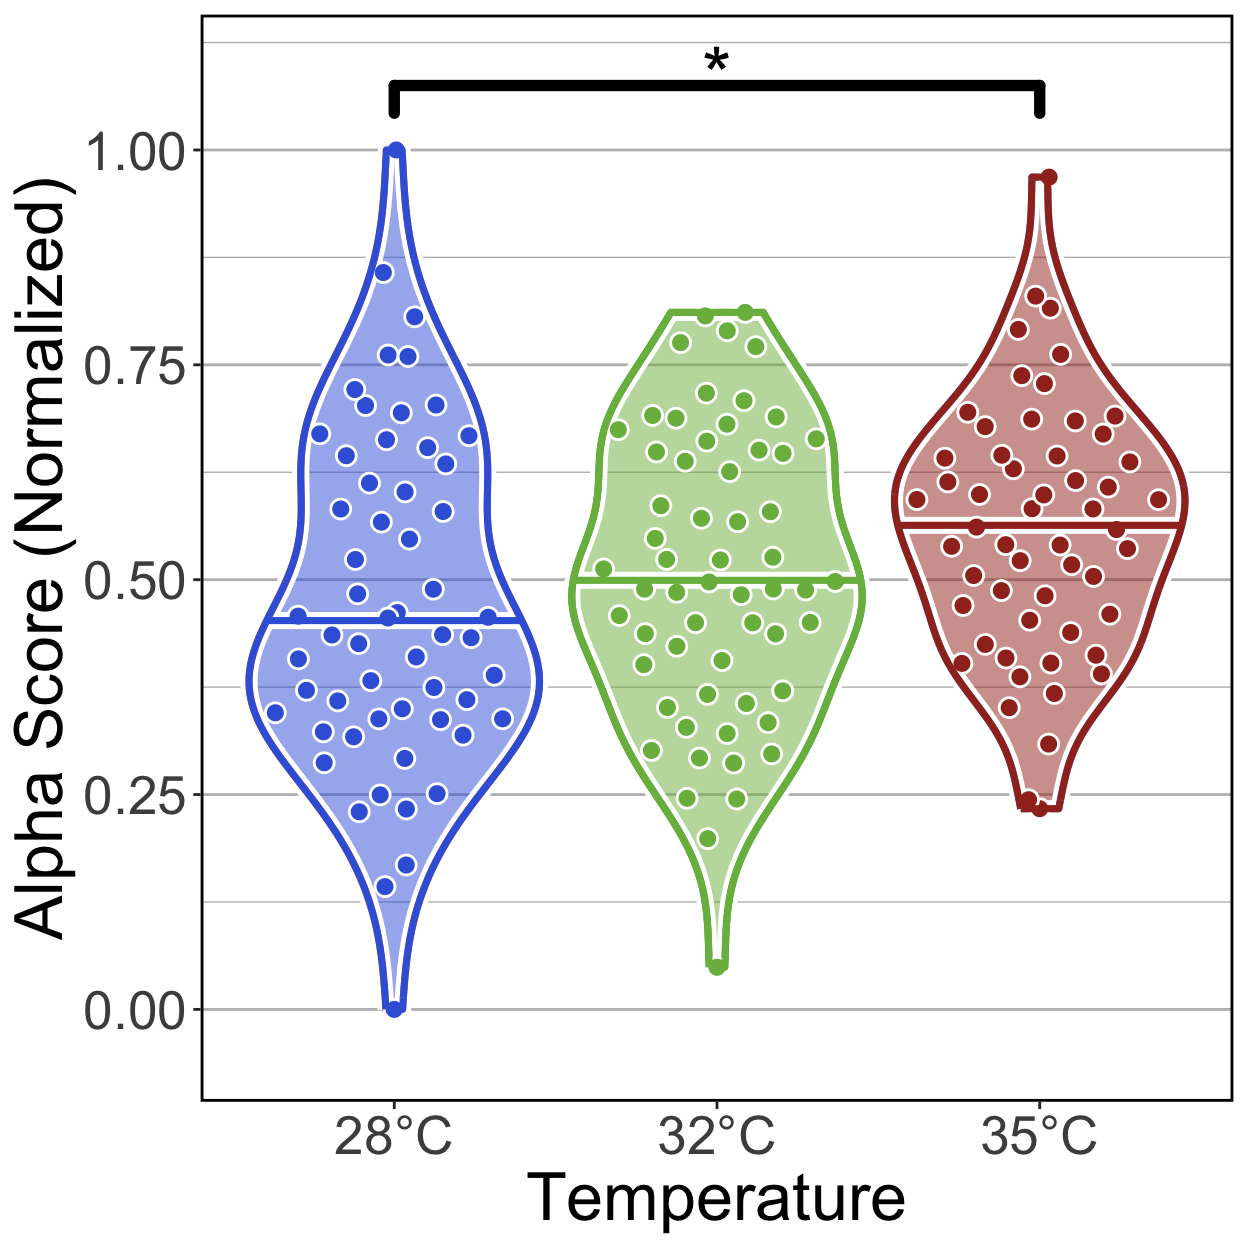
\includegraphics[keepaspectratio]{Results_Overview_files/figure-latex/plots-2A-1.pdf}}

\subparagraph{Tables}\label{tables}

(hide)

Click on tabs to display tables. Scroll to see additional rows.

GLM

\begin{longtable}{lrrrrl}
\caption*{
{\large GLM Results} \\ 
{\small glm(Alpha.Score \textasciitilde{} Temperature); Unexposed fish}
} \\ 
\toprule
term & estimate & std.error & statistic & p.value & p.adj.sig \\ 
\midrule\addlinespace[2.5pt]
\multicolumn{6}{l}{Shannon} \\ 
\midrule\addlinespace[2.5pt]
(Intercept) & $-0.754$ & $0.091$ & $-8.309$ & <0.001 & **** \\ 
Temperature32 & $0.051$ & $0.127$ & $0.400$ & $\geq$0.25 & ns \\ 
Temperature35 & $0.054$ & $0.129$ & $0.421$ & $\geq$0.25 & ns \\ 
\midrule\addlinespace[2.5pt]
\multicolumn{6}{l}{Simpson} \\ 
\midrule\addlinespace[2.5pt]
(Intercept) & $-0.101$ & $0.092$ & $-1.103$ & $\geq$0.25 & ns \\ 
Temperature32 & $0.132$ & $0.128$ & $1.030$ & $\geq$0.25 & ns \\ 
Temperature35 & $0.340$ & $0.131$ & $2.591$ & $0.010$ & * \\ 
\midrule\addlinespace[2.5pt]
\multicolumn{6}{l}{Richness} \\ 
\midrule\addlinespace[2.5pt]
(Intercept) & $-0.231$ & $0.075$ & $-3.079$ & $0.002$ & ** \\ 
Temperature32 & $0.047$ & $0.105$ & $0.446$ & $\geq$0.25 & ns \\ 
Temperature35 & $-0.473$ & $0.110$ & $-4.299$ & <0.001 & **** \\ 
\midrule\addlinespace[2.5pt]
\multicolumn{6}{l}{Phylogenetic} \\ 
\midrule\addlinespace[2.5pt]
(Intercept) & $-0.255$ & $0.072$ & $-3.540$ & <0.001 & *** \\ 
Temperature32 & $0.068$ & $0.101$ & $0.673$ & $\geq$0.25 & ns \\ 
Temperature35 & $-0.475$ & $0.106$ & $-4.482$ & <0.001 & **** \\ 
\bottomrule
\end{longtable}

ANOVA

\begin{longtable}{lrrrl}
\caption*{
{\large ANOVA of GLM} \\ 
{\small ANOVA(GLM(Alpha.Score \textasciitilde{} Temperature), type = 2); Unexposed fish}
} \\ 
\toprule
term & statistic & df & p.value & sig \\ 
\midrule\addlinespace[2.5pt]
\multicolumn{5}{l}{Shannon} \\ 
\midrule\addlinespace[2.5pt]
Temperature & $0.225$ & $2.000$ & $\geq$0.25 & ns \\ 
\midrule\addlinespace[2.5pt]
\multicolumn{5}{l}{Simpson} \\ 
\midrule\addlinespace[2.5pt]
Temperature & $6.830$ & $2.000$ & $0.033$ & * \\ 
\midrule\addlinespace[2.5pt]
\multicolumn{5}{l}{Richness} \\ 
\midrule\addlinespace[2.5pt]
Temperature & $27.512$ & $2.000$ & <0.001 & **** \\ 
\midrule\addlinespace[2.5pt]
\multicolumn{5}{l}{Phylogenetic} \\ 
\midrule\addlinespace[2.5pt]
Temperature & $31.449$ & $2.000$ & <0.001 & **** \\ 
\bottomrule
\end{longtable}

Tukey

\begin{longtable}{llrrrrrrl}
\caption*{
{\large Pairwise Tukey's HSD, p.adj: Dunnett} \\ 
{\small Tukey(Alpha.Score \textasciitilde{} Temperature); Unexposed fish}
} \\ 
\toprule
term & .y. & group1 & group2 & estimate & std.error & statistic & adj.p.value & Variable \\ 
\midrule\addlinespace[2.5pt]
\multicolumn{9}{l}{Shannon} \\ 
\midrule\addlinespace[2.5pt]
Temperature & Alpha.Score & 32 & 28 & $0.051$ & $0.127$ & $0.400$ & $\geq$0.25 & Temperature \\ 
Temperature & Alpha.Score & 35 & 28 & $0.054$ & $0.129$ & $0.421$ & $\geq$0.25 & Temperature \\ 
Temperature & Alpha.Score & 35 & 32 & $0.004$ & $0.127$ & $0.029$ & $\geq$0.25 & Temperature \\ 
\midrule\addlinespace[2.5pt]
\multicolumn{9}{l}{Simpson} \\ 
\midrule\addlinespace[2.5pt]
Temperature & Alpha.Score & 32 & 28 & $0.132$ & $0.128$ & $1.030$ & $\geq$0.25 & Temperature \\ 
Temperature & Alpha.Score & 35 & 28 & $0.340$ & $0.131$ & $2.591$ & $0.026$ & Temperature \\ 
Temperature & Alpha.Score & 35 & 32 & $0.207$ & $0.130$ & $1.596$ & $0.247$ & Temperature \\ 
\midrule\addlinespace[2.5pt]
\multicolumn{9}{l}{Richness} \\ 
\midrule\addlinespace[2.5pt]
Temperature & Alpha.Score & 32 & 28 & $0.047$ & $0.105$ & $0.446$ & $\geq$0.25 & Temperature \\ 
Temperature & Alpha.Score & 35 & 28 & $-0.473$ & $0.110$ & $-4.299$ & <0.001 & Temperature \\ 
Temperature & Alpha.Score & 35 & 32 & $-0.520$ & $0.109$ & $-4.768$ & <0.001 & Temperature \\ 
\midrule\addlinespace[2.5pt]
\multicolumn{9}{l}{Phylogenetic} \\ 
\midrule\addlinespace[2.5pt]
Temperature & Alpha.Score & 32 & 28 & $0.068$ & $0.101$ & $0.673$ & $\geq$0.25 & Temperature \\ 
Temperature & Alpha.Score & 35 & 28 & $-0.475$ & $0.106$ & $-4.482$ & <0.001 & Temperature \\ 
Temperature & Alpha.Score & 35 & 32 & $-0.543$ & $0.105$ & $-5.172$ & <0.001 & Temperature \\ 
\bottomrule
\end{longtable}

\subparagraph{Addl. Metrics}\label{addl.-metrics}

\paragraph{2B)}\label{b}

\pandocbounded{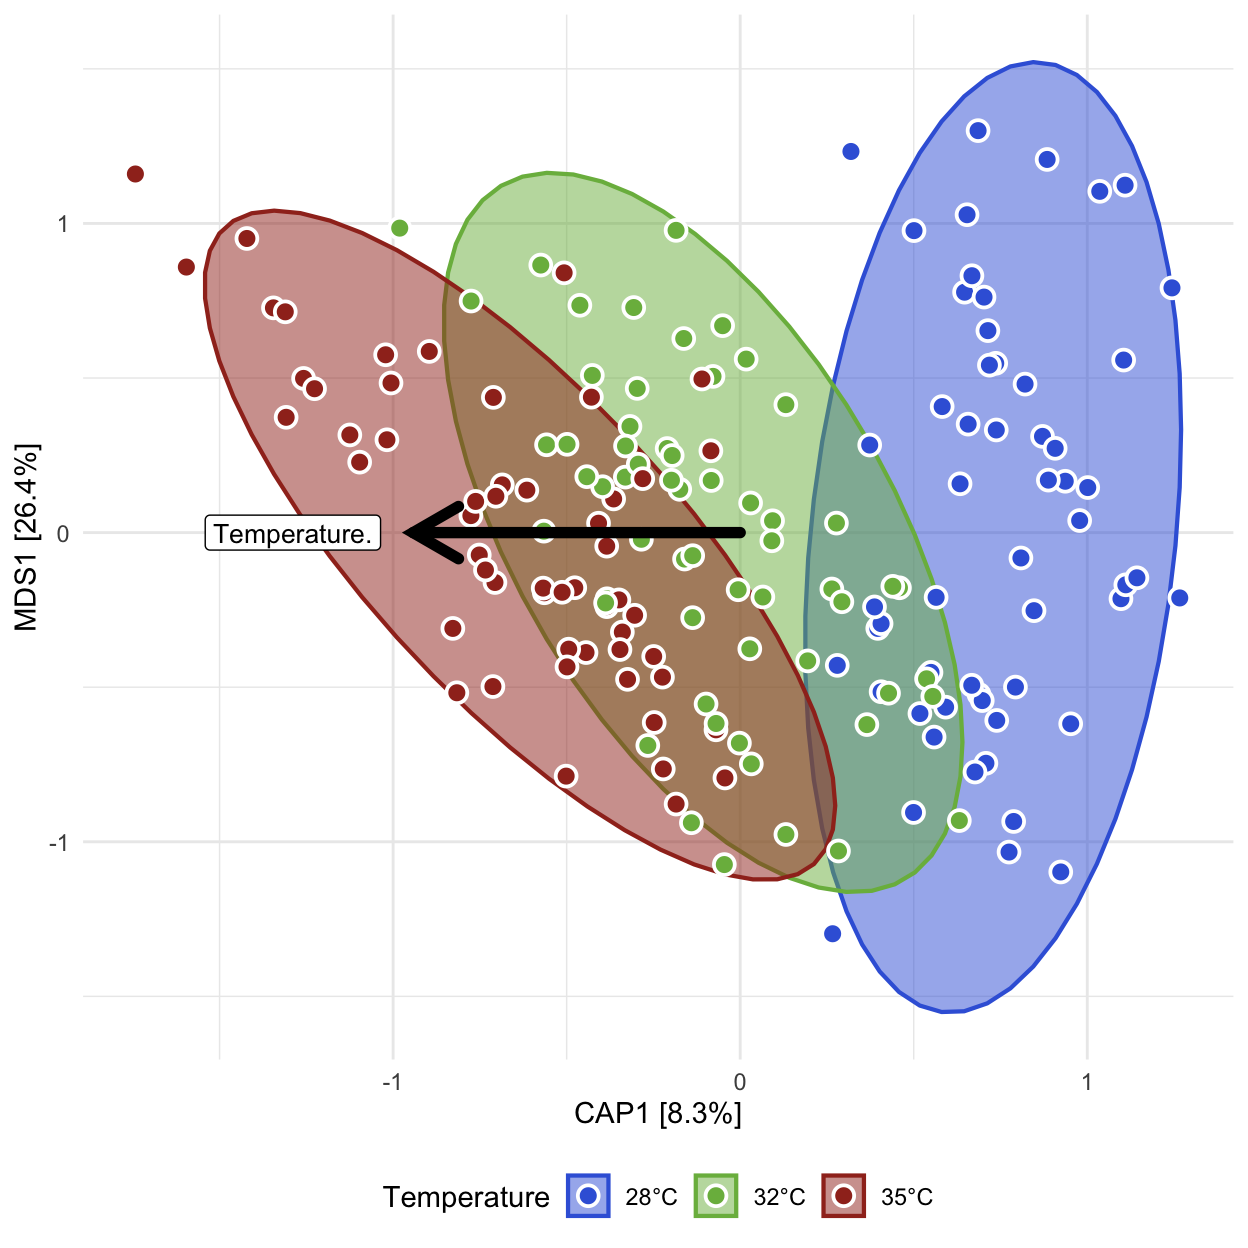
\includegraphics[keepaspectratio]{Results_Overview_files/figure-latex/plots-2B-1.pdf}}

\subparagraph{Tables}\label{tables-1}

(hide)

Click on tabs to display tables. Scroll to see additional rows.

ADONIS2

\begin{longtable}{lrrrrrr}
\caption*{
{\large ADONIS2} \\ 
{\small adonis2(Beta Distance \textasciitilde{} Temperature); Unexposed fish}
} \\ 
\toprule
term & df & SumOfSqs & R2 & statistic & p.value & sig \\ 
\midrule\addlinespace[2.5pt]
\multicolumn{7}{l}{bray} \\ 
\midrule\addlinespace[2.5pt]
Temperature & $2.000$ & $2.294$ & $0.133$ & $12.900$ & $0.001$ & *** \\ 
Residual & $168.000$ & $14.936$ & $0.867$ & NA & NA & NA \\ 
Total & $170.000$ & $17.229$ & $1.000$ & NA & NA & NA \\ 
\midrule\addlinespace[2.5pt]
\multicolumn{7}{l}{canberra} \\ 
\midrule\addlinespace[2.5pt]
Temperature & $2.000$ & $3.862$ & $0.099$ & $9.178$ & $0.001$ & *** \\ 
Residual & $168.000$ & $35.344$ & $0.901$ & NA & NA & NA \\ 
Total & $170.000$ & $39.206$ & $1.000$ & NA & NA & NA \\ 
\midrule\addlinespace[2.5pt]
\multicolumn{7}{l}{gunifrac} \\ 
\midrule\addlinespace[2.5pt]
Temperature & $2.000$ & $1.422$ & $0.102$ & $9.566$ & $0.001$ & *** \\ 
Residual & $168.000$ & $12.485$ & $0.898$ & NA & NA & NA \\ 
Total & $170.000$ & $13.907$ & $1.000$ & NA & NA & NA \\ 
\bottomrule
\end{longtable}

Dispersion (ANOVA)

\begin{longtable}{lrrrrrl}
\caption*{
{\large ANOVA: Homogeneity of Dispersion} \\ 
{\small ANOVA(Beta Disperson \textasciitilde{} Temperature); Unexposed fish}
} \\ 
\toprule
term & df & sumsq & meansq & statistic & p.value & sig \\ 
\midrule\addlinespace[2.5pt]
\multicolumn{7}{l}{bray} \\ 
\midrule\addlinespace[2.5pt]
Temperature & $2.000$ & $0.008$ & $0.004$ & $0.386$ & $\geq$0.25 & ns \\ 
Residual & $168.000$ & $1.771$ & $0.011$ & NA & NA & NA \\ 
\midrule\addlinespace[2.5pt]
\multicolumn{7}{l}{canberra} \\ 
\midrule\addlinespace[2.5pt]
Temperature & $2.000$ & $0.008$ & $0.004$ & $0.873$ & $\geq$0.25 & ns \\ 
Residual & $168.000$ & $0.759$ & $0.005$ & NA & NA & NA \\ 
\midrule\addlinespace[2.5pt]
\multicolumn{7}{l}{gunifrac} \\ 
\midrule\addlinespace[2.5pt]
Temperature & $2.000$ & $0.005$ & $0.003$ & $0.369$ & $\geq$0.25 & ns \\ 
Residual & $168.000$ & $1.143$ & $0.007$ & NA & NA & NA \\ 
\bottomrule
\end{longtable}

Dispersion (Tukey)

\begin{longtable}{llrrrrrrl}
\caption*{
{\large Tukey: Homogeneity of Dispersion} \\ 
{\small Tukey(Beta Disperson \textasciitilde{} Temperature); Unexposed fish}
} \\ 
\toprule
.y. & term & group1 & group2 & estimate & conf.low & conf.high & adj.p.value & sig \\ 
\midrule\addlinespace[2.5pt]
\multicolumn{9}{l}{bray} \\ 
\midrule\addlinespace[2.5pt]
Distance & Temperature & 32 & 28 & $-0.011$ & $-0.056$ & $0.034$ & $\geq$0.25 & ns \\ 
Distance & Temperature & 35 & 28 & $0.005$ & $-0.041$ & $0.051$ & $\geq$0.25 & ns \\ 
Distance & Temperature & 35 & 32 & $0.016$ & $-0.029$ & $0.062$ & $\geq$0.25 & ns \\ 
\midrule\addlinespace[2.5pt]
\multicolumn{9}{l}{canberra} \\ 
\midrule\addlinespace[2.5pt]
Distance & Temperature & 32 & 28 & $-0.001$ & $-0.031$ & $0.028$ & $\geq$0.25 & ns \\ 
Distance & Temperature & 35 & 28 & $0.014$ & $-0.016$ & $0.044$ & $\geq$0.25 & ns \\ 
Distance & Temperature & 35 & 32 & $0.015$ & $-0.015$ & $0.045$ & $\geq$0.25 & ns \\ 
\midrule\addlinespace[2.5pt]
\multicolumn{9}{l}{gunifrac} \\ 
\midrule\addlinespace[2.5pt]
Distance & Temperature & 32 & 28 & $-0.013$ & $-0.049$ & $0.023$ & $\geq$0.25 & ns \\ 
Distance & Temperature & 35 & 28 & $-0.004$ & $-0.040$ & $0.033$ & $\geq$0.25 & ns \\ 
Distance & Temperature & 35 & 32 & $0.009$ & $-0.027$ & $0.046$ & $\geq$0.25 & ns \\ 
\bottomrule
\end{longtable}

\subparagraph{Addl. Metrics}\label{addl.-metrics-1}

\paragraph{2C)}\label{c}

\pandocbounded{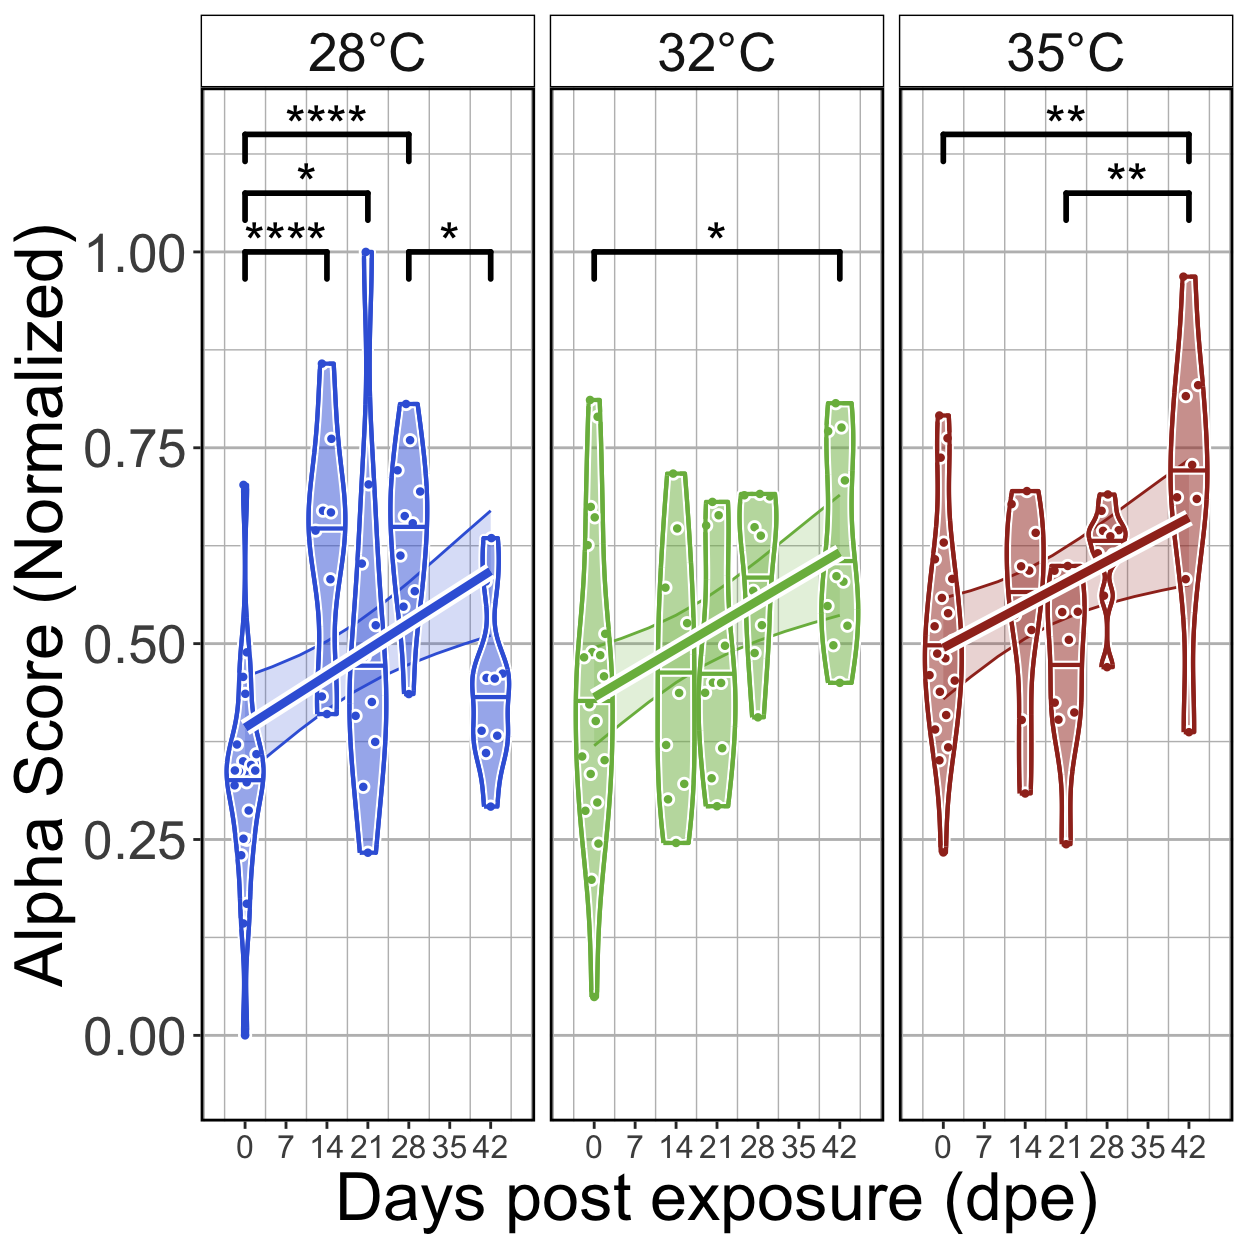
\includegraphics[keepaspectratio]{Results_Overview_files/figure-latex/plots-2C-1.pdf}}

\subparagraph{Tables}\label{tables-2}

(hide)

Click on tabs to display tables. Scroll to see additional rows.

GLM

\begin{longtable}{lrrrrl}
\caption*{
{\large GLM Results} \\ 
{\small glm(Alpha.Score \textasciitilde{} Temperature*DPE); Unexposed fish}
} \\ 
\toprule
term & estimate & std.error & statistic & p.value & p.adj.sig \\ 
\midrule\addlinespace[2.5pt]
\multicolumn{6}{l}{Shannon} \\ 
\midrule\addlinespace[2.5pt]
(Intercept) & $-1.074$ & $0.138$ & $-7.754$ & <0.001 & **** \\ 
Temperature32 & $0.075$ & $0.193$ & $0.386$ & $\geq$0.25 & ns \\ 
Temperature35 & $0.154$ & $0.193$ & $0.797$ & $\geq$0.25 & ns \\ 
DPE & $0.018$ & $0.006$ & $3.086$ & $0.002$ & ** \\ 
Temperature32:DPE & $-0.001$ & $0.008$ & $-0.170$ & $\geq$0.25 & ns \\ 
Temperature35:DPE & $-0.005$ & $0.008$ & $-0.585$ & $\geq$0.25 & ns \\ 
\midrule\addlinespace[2.5pt]
\multicolumn{6}{l}{Simpson} \\ 
\midrule\addlinespace[2.5pt]
(Intercept) & $-0.433$ & $0.134$ & $-3.245$ & $0.001$ & ** \\ 
Temperature32 & $0.157$ & $0.186$ & $0.841$ & $\geq$0.25 & ns \\ 
Temperature35 & $0.408$ & $0.187$ & $2.177$ & $0.031$ & * \\ 
DPE & $0.019$ & $0.006$ & $3.293$ & $0.001$ & ** \\ 
Temperature32:DPE & $-0.001$ & $0.008$ & $-0.173$ & $\geq$0.25 & ns \\ 
Temperature35:DPE & $-0.003$ & $0.008$ & $-0.343$ & $\geq$0.25 & ns \\ 
\midrule\addlinespace[2.5pt]
\multicolumn{6}{l}{Richness} \\ 
\midrule\addlinespace[2.5pt]
(Intercept) & $-0.651$ & $0.108$ & $-6.017$ & <0.001 & **** \\ 
Temperature32 & $0.189$ & $0.150$ & $1.257$ & $0.211$ & ns \\ 
Temperature35 & $-0.059$ & $0.154$ & $-0.383$ & $\geq$0.25 & ns \\ 
DPE & $0.024$ & $0.005$ & $5.137$ & <0.001 & **** \\ 
Temperature32:DPE & $-0.008$ & $0.006$ & $-1.251$ & $0.213$ & ns \\ 
Temperature35:DPE & $-0.024$ & $0.007$ & $-3.476$ & <0.001 & *** \\ 
\midrule\addlinespace[2.5pt]
\multicolumn{6}{l}{Phylogenetic} \\ 
\midrule\addlinespace[2.5pt]
(Intercept) & $-0.709$ & $0.102$ & $-6.970$ & <0.001 & **** \\ 
Temperature32 & $0.237$ & $0.141$ & $1.682$ & $0.095$ & ns \\ 
Temperature35 & $0.010$ & $0.144$ & $0.072$ & $\geq$0.25 & ns \\ 
DPE & $0.026$ & $0.004$ & $5.907$ & <0.001 & **** \\ 
Temperature32:DPE & $-0.010$ & $0.006$ & $-1.579$ & $0.116$ & ns \\ 
Temperature35:DPE & $-0.028$ & $0.006$ & $-4.344$ & <0.001 & **** \\ 
\bottomrule
\end{longtable}

ANOVA

\begin{longtable}{lrrrl}
\caption*{
{\large ANOVA of GLM} \\ 
{\small ANOVA(GLM(Alpha.Score \textasciitilde{} Temperature*Time), type = 2); Unexposed fish}
} \\ 
\toprule
term & statistic & df & p.value & sig \\ 
\midrule\addlinespace[2.5pt]
\multicolumn{5}{l}{Shannon} \\ 
\midrule\addlinespace[2.5pt]
Temperature & $0.322$ & $2.000$ & $\geq$0.25 & ns \\ 
DPE & $22.895$ & $1.000$ & <0.001 & **** \\ 
Temperature:DPE & $0.363$ & $2.000$ & $\geq$0.25 & ns \\ 
\midrule\addlinespace[2.5pt]
\multicolumn{5}{l}{Simpson} \\ 
\midrule\addlinespace[2.5pt]
Temperature & $8.551$ & $2.000$ & $0.014$ & * \\ 
DPE & $28.161$ & $1.000$ & <0.001 & **** \\ 
Temperature:DPE & $0.118$ & $2.000$ & $\geq$0.25 & ns \\ 
\midrule\addlinespace[2.5pt]
\multicolumn{5}{l}{Richness} \\ 
\midrule\addlinespace[2.5pt]
Temperature & $31.759$ & $2.000$ & <0.001 & **** \\ 
DPE & $27.201$ & $1.000$ & <0.001 & **** \\ 
Temperature:DPE & $12.460$ & $2.000$ & $0.002$ & ** \\ 
\midrule\addlinespace[2.5pt]
\multicolumn{5}{l}{Phylogenetic} \\ 
\midrule\addlinespace[2.5pt]
Temperature & $38.358$ & $2.000$ & <0.001 & **** \\ 
DPE & $31.813$ & $1.000$ & <0.001 & **** \\ 
Temperature:DPE & $19.500$ & $2.000$ & <0.001 & **** \\ 
\bottomrule
\end{longtable}

Tukey

\begin{longtable}{cllrrrrrrlc}
\caption*{
{\large Pairwise Tukey's HSD, p.adj: Dunnett} \\ 
{\small Tukey(Alpha.Score \textasciitilde{} Temperature*Time); Unexposed fish}
} \\ 
\toprule
Temperature & .y. & term & group1 & group2 & estimate & std.error & statistic & adj.p.value & Variable & Group \\ 
\midrule\addlinespace[2.5pt]
\multicolumn{11}{l}{Shannon} \\ 
\midrule\addlinespace[2.5pt]
28 & Alpha.Score & DPE & 14 & 0 & $1.065$ & $0.294$ & $3.625$ & $0.003$ & DPE & 28 \\ 
28 & Alpha.Score & DPE & 21 & 0 & $0.722$ & $0.281$ & $2.566$ & $0.076$ & DPE & 28 \\ 
28 & Alpha.Score & DPE & 28 & 0 & $1.187$ & $0.274$ & $4.335$ & <0.001 & DPE & 28 \\ 
28 & Alpha.Score & DPE & 42 & 0 & $0.548$ & $0.296$ & $1.853$ & $\geq$0.25 & DPE & 28 \\ 
28 & Alpha.Score & DPE & 21 & 14 & $-0.343$ & $0.317$ & $-1.083$ & $\geq$0.25 & DPE & 28 \\ 
28 & Alpha.Score & DPE & 28 & 14 & $0.122$ & $0.310$ & $0.392$ & $\geq$0.25 & DPE & 28 \\ 
28 & Alpha.Score & DPE & 42 & 14 & $-0.517$ & $0.330$ & $-1.567$ & $\geq$0.25 & DPE & 28 \\ 
28 & Alpha.Score & DPE & 28 & 21 & $0.465$ & $0.299$ & $1.558$ & $\geq$0.25 & DPE & 28 \\ 
28 & Alpha.Score & DPE & 42 & 21 & $-0.174$ & $0.319$ & $-0.545$ & $\geq$0.25 & DPE & 28 \\ 
28 & Alpha.Score & DPE & 42 & 28 & $-0.639$ & $0.312$ & $-2.045$ & $0.243$ & DPE & 28 \\ 
32 & Alpha.Score & DPE & 14 & 0 & $0.006$ & $0.250$ & $0.022$ & $\geq$0.25 & DPE & 32 \\ 
32 & Alpha.Score & DPE & 21 & 0 & $0.112$ & $0.247$ & $0.452$ & $\geq$0.25 & DPE & 32 \\ 
32 & Alpha.Score & DPE & 28 & 0 & $0.420$ & $0.248$ & $1.695$ & $\geq$0.25 & DPE & 32 \\ 
32 & Alpha.Score & DPE & 42 & 0 & $0.694$ & $0.236$ & $2.943$ & $0.026$ & DPE & 32 \\ 
32 & Alpha.Score & DPE & 21 & 14 & $0.106$ & $0.286$ & $0.371$ & $\geq$0.25 & DPE & 32 \\ 
32 & Alpha.Score & DPE & 28 & 14 & $0.414$ & $0.287$ & $1.445$ & $\geq$0.25 & DPE & 32 \\ 
32 & Alpha.Score & DPE & 42 & 14 & $0.688$ & $0.276$ & $2.490$ & $0.092$ & DPE & 32 \\ 
32 & Alpha.Score & DPE & 28 & 21 & $0.308$ & $0.283$ & $1.087$ & $\geq$0.25 & DPE & 32 \\ 
32 & Alpha.Score & DPE & 42 & 21 & $0.582$ & $0.273$ & $2.131$ & $0.205$ & DPE & 32 \\ 
32 & Alpha.Score & DPE & 42 & 28 & $0.274$ & $0.274$ & $1.001$ & $\geq$0.25 & DPE & 32 \\ 
35 & Alpha.Score & DPE & 14 & 0 & $-0.006$ & $0.210$ & $-0.027$ & $\geq$0.25 & DPE & 35 \\ 
35 & Alpha.Score & DPE & 21 & 0 & $-0.249$ & $0.218$ & $-1.145$ & $\geq$0.25 & DPE & 35 \\ 
35 & Alpha.Score & DPE & 28 & 0 & $0.232$ & $0.204$ & $1.138$ & $\geq$0.25 & DPE & 35 \\ 
35 & Alpha.Score & DPE & 42 & 0 & $0.661$ & $0.207$ & $3.194$ & $0.012$ & DPE & 35 \\ 
35 & Alpha.Score & DPE & 21 & 14 & $-0.243$ & $0.253$ & $-0.962$ & $\geq$0.25 & DPE & 35 \\ 
35 & Alpha.Score & DPE & 28 & 14 & $0.238$ & $0.242$ & $0.985$ & $\geq$0.25 & DPE & 35 \\ 
35 & Alpha.Score & DPE & 42 & 14 & $0.667$ & $0.244$ & $2.733$ & $0.049$ & DPE & 35 \\ 
35 & Alpha.Score & DPE & 28 & 21 & $0.481$ & $0.248$ & $1.938$ & $\geq$0.25 & DPE & 35 \\ 
35 & Alpha.Score & DPE & 42 & 21 & $0.910$ & $0.251$ & $3.628$ & $0.003$ & DPE & 35 \\ 
35 & Alpha.Score & DPE & 42 & 28 & $0.429$ & $0.239$ & $1.792$ & $\geq$0.25 & DPE & 35 \\ 
\midrule\addlinespace[2.5pt]
\multicolumn{11}{l}{Simpson} \\ 
\midrule\addlinespace[2.5pt]
28 & Alpha.Score & DPE & 14 & 0 & $1.256$ & $0.273$ & $4.611$ & <0.001 & DPE & 28 \\ 
28 & Alpha.Score & DPE & 21 & 0 & $0.761$ & $0.247$ & $3.076$ & $0.018$ & DPE & 28 \\ 
28 & Alpha.Score & DPE & 28 & 0 & $1.334$ & $0.254$ & $5.241$ & <0.001 & DPE & 28 \\ 
28 & Alpha.Score & DPE & 42 & 0 & $0.514$ & $0.257$ & $2.002$ & $\geq$0.25 & DPE & 28 \\ 
28 & Alpha.Score & DPE & 21 & 14 & $-0.496$ & $0.302$ & $-1.644$ & $\geq$0.25 & DPE & 28 \\ 
28 & Alpha.Score & DPE & 28 & 14 & $0.077$ & $0.308$ & $0.251$ & $\geq$0.25 & DPE & 28 \\ 
28 & Alpha.Score & DPE & 42 & 14 & $-0.742$ & $0.310$ & $-2.398$ & $0.114$ & DPE & 28 \\ 
28 & Alpha.Score & DPE & 28 & 21 & $0.573$ & $0.285$ & $2.008$ & $\geq$0.25 & DPE & 28 \\ 
28 & Alpha.Score & DPE & 42 & 21 & $-0.246$ & $0.288$ & $-0.857$ & $\geq$0.25 & DPE & 28 \\ 
28 & Alpha.Score & DPE & 42 & 28 & $-0.819$ & $0.294$ & $-2.789$ & $0.042$ & DPE & 28 \\ 
32 & Alpha.Score & DPE & 14 & 0 & $0.065$ & $0.249$ & $0.261$ & $\geq$0.25 & DPE & 32 \\ 
32 & Alpha.Score & DPE & 21 & 0 & $0.142$ & $0.249$ & $0.569$ & $\geq$0.25 & DPE & 32 \\ 
32 & Alpha.Score & DPE & 28 & 0 & $0.592$ & $0.261$ & $2.272$ & $0.152$ & DPE & 32 \\ 
32 & Alpha.Score & DPE & 42 & 0 & $0.724$ & $0.254$ & $2.850$ & $0.035$ & DPE & 32 \\ 
32 & Alpha.Score & DPE & 21 & 14 & $0.077$ & $0.287$ & $0.267$ & $\geq$0.25 & DPE & 32 \\ 
32 & Alpha.Score & DPE & 28 & 14 & $0.527$ & $0.297$ & $1.773$ & $\geq$0.25 & DPE & 32 \\ 
32 & Alpha.Score & DPE & 42 & 14 & $0.659$ & $0.292$ & $2.260$ & $0.156$ & DPE & 32 \\ 
32 & Alpha.Score & DPE & 28 & 21 & $0.451$ & $0.297$ & $1.517$ & $\geq$0.25 & DPE & 32 \\ 
32 & Alpha.Score & DPE & 42 & 21 & $0.582$ & $0.291$ & $1.999$ & $\geq$0.25 & DPE & 32 \\ 
32 & Alpha.Score & DPE & 42 & 28 & $0.132$ & $0.302$ & $0.436$ & $\geq$0.25 & DPE & 32 \\ 
35 & Alpha.Score & DPE & 14 & 0 & $0.149$ & $0.219$ & $0.683$ & $\geq$0.25 & DPE & 35 \\ 
35 & Alpha.Score & DPE & 21 & 0 & $-0.167$ & $0.218$ & $-0.766$ & $\geq$0.25 & DPE & 35 \\ 
35 & Alpha.Score & DPE & 28 & 0 & $0.413$ & $0.222$ & $1.858$ & $\geq$0.25 & DPE & 35 \\ 
35 & Alpha.Score & DPE & 42 & 0 & $0.836$ & $0.244$ & $3.431$ & $0.005$ & DPE & 35 \\ 
35 & Alpha.Score & DPE & 21 & 14 & $-0.316$ & $0.257$ & $-1.232$ & $\geq$0.25 & DPE & 35 \\ 
35 & Alpha.Score & DPE & 28 & 14 & $0.263$ & $0.260$ & $1.013$ & $\geq$0.25 & DPE & 35 \\ 
35 & Alpha.Score & DPE & 42 & 14 & $0.687$ & $0.279$ & $2.465$ & $0.097$ & DPE & 35 \\ 
35 & Alpha.Score & DPE & 28 & 21 & $0.579$ & $0.260$ & $2.233$ & $0.165$ & DPE & 35 \\ 
35 & Alpha.Score & DPE & 42 & 21 & $1.003$ & $0.278$ & $3.604$ & $0.003$ & DPE & 35 \\ 
35 & Alpha.Score & DPE & 42 & 28 & $0.424$ & $0.282$ & $1.506$ & $\geq$0.25 & DPE & 35 \\ 
\midrule\addlinespace[2.5pt]
\multicolumn{11}{l}{Richness} \\ 
\midrule\addlinespace[2.5pt]
28 & Alpha.Score & DPE & 14 & 0 & $0.432$ & $0.236$ & $1.836$ & $\geq$0.25 & DPE & 28 \\ 
28 & Alpha.Score & DPE & 21 & 0 & $0.550$ & $0.218$ & $2.526$ & $0.084$ & DPE & 28 \\ 
28 & Alpha.Score & DPE & 28 & 0 & $0.767$ & $0.218$ & $3.525$ & $0.004$ & DPE & 28 \\ 
28 & Alpha.Score & DPE & 42 & 0 & $0.970$ & $0.227$ & $4.278$ & <0.001 & DPE & 28 \\ 
28 & Alpha.Score & DPE & 21 & 14 & $0.118$ & $0.263$ & $0.449$ & $\geq$0.25 & DPE & 28 \\ 
28 & Alpha.Score & DPE & 28 & 14 & $0.335$ & $0.262$ & $1.275$ & $\geq$0.25 & DPE & 28 \\ 
28 & Alpha.Score & DPE & 42 & 14 & $0.537$ & $0.270$ & $1.990$ & $\geq$0.25 & DPE & 28 \\ 
28 & Alpha.Score & DPE & 28 & 21 & $0.217$ & $0.247$ & $0.880$ & $\geq$0.25 & DPE & 28 \\ 
28 & Alpha.Score & DPE & 42 & 21 & $0.419$ & $0.255$ & $1.647$ & $\geq$0.25 & DPE & 28 \\ 
28 & Alpha.Score & DPE & 42 & 28 & $0.203$ & $0.254$ & $0.796$ & $\geq$0.25 & DPE & 28 \\ 
32 & Alpha.Score & DPE & 14 & 0 & $-0.170$ & $0.177$ & $-0.965$ & $\geq$0.25 & DPE & 32 \\ 
32 & Alpha.Score & DPE & 21 & 0 & $-0.026$ & $0.175$ & $-0.147$ & $\geq$0.25 & DPE & 32 \\ 
32 & Alpha.Score & DPE & 28 & 0 & $0.187$ & $0.180$ & $1.041$ & $\geq$0.25 & DPE & 32 \\ 
32 & Alpha.Score & DPE & 42 & 0 & $0.769$ & $0.176$ & $4.359$ & <0.001 & DPE & 32 \\ 
32 & Alpha.Score & DPE & 21 & 14 & $0.145$ & $0.204$ & $0.711$ & $\geq$0.25 & DPE & 32 \\ 
32 & Alpha.Score & DPE & 28 & 14 & $0.358$ & $0.208$ & $1.721$ & $\geq$0.25 & DPE & 32 \\ 
32 & Alpha.Score & DPE & 42 & 14 & $0.939$ & $0.205$ & $4.585$ & <0.001 & DPE & 32 \\ 
32 & Alpha.Score & DPE & 28 & 21 & $0.213$ & $0.206$ & $1.031$ & $\geq$0.25 & DPE & 32 \\ 
32 & Alpha.Score & DPE & 42 & 21 & $0.794$ & $0.203$ & $3.906$ & <0.001 & DPE & 32 \\ 
32 & Alpha.Score & DPE & 42 & 28 & $0.581$ & $0.208$ & $2.801$ & $0.040$ & DPE & 32 \\ 
35 & Alpha.Score & DPE & 14 & 0 & $-0.560$ & $0.214$ & $-2.612$ & $0.067$ & DPE & 35 \\ 
35 & Alpha.Score & DPE & 21 & 0 & $-0.551$ & $0.214$ & $-2.578$ & $0.073$ & DPE & 35 \\ 
35 & Alpha.Score & DPE & 28 & 0 & $0.110$ & $0.196$ & $0.561$ & $\geq$0.25 & DPE & 35 \\ 
35 & Alpha.Score & DPE & 42 & 0 & $0.007$ & $0.206$ & $0.036$ & $\geq$0.25 & DPE & 35 \\ 
35 & Alpha.Score & DPE & 21 & 14 & $0.008$ & $0.259$ & $0.032$ & $\geq$0.25 & DPE & 35 \\ 
35 & Alpha.Score & DPE & 28 & 14 & $0.670$ & $0.245$ & $2.733$ & $0.048$ & DPE & 35 \\ 
35 & Alpha.Score & DPE & 42 & 14 & $0.567$ & $0.253$ & $2.240$ & $0.162$ & DPE & 35 \\ 
35 & Alpha.Score & DPE & 28 & 21 & $0.661$ & $0.245$ & $2.702$ & $0.052$ & DPE & 35 \\ 
35 & Alpha.Score & DPE & 42 & 21 & $0.559$ & $0.253$ & $2.210$ & $0.173$ & DPE & 35 \\ 
35 & Alpha.Score & DPE & 42 & 28 & $-0.103$ & $0.238$ & $-0.431$ & $\geq$0.25 & DPE & 35 \\ 
\midrule\addlinespace[2.5pt]
\multicolumn{11}{l}{Phylogenetic} \\ 
\midrule\addlinespace[2.5pt]
28 & Alpha.Score & DPE & 14 & 0 & $0.452$ & $0.229$ & $1.969$ & $\geq$0.25 & DPE & 28 \\ 
28 & Alpha.Score & DPE & 21 & 0 & $0.679$ & $0.211$ & $3.210$ & $0.011$ & DPE & 28 \\ 
28 & Alpha.Score & DPE & 28 & 0 & $0.872$ & $0.212$ & $4.120$ & <0.001 & DPE & 28 \\ 
28 & Alpha.Score & DPE & 42 & 0 & $1.012$ & $0.220$ & $4.602$ & <0.001 & DPE & 28 \\ 
28 & Alpha.Score & DPE & 21 & 14 & $0.227$ & $0.254$ & $0.893$ & $\geq$0.25 & DPE & 28 \\ 
28 & Alpha.Score & DPE & 28 & 14 & $0.420$ & $0.254$ & $1.651$ & $\geq$0.25 & DPE & 28 \\ 
28 & Alpha.Score & DPE & 42 & 14 & $0.560$ & $0.261$ & $2.142$ & $0.200$ & DPE & 28 \\ 
28 & Alpha.Score & DPE & 28 & 21 & $0.193$ & $0.238$ & $0.809$ & $\geq$0.25 & DPE & 28 \\ 
28 & Alpha.Score & DPE & 42 & 21 & $0.333$ & $0.246$ & $1.353$ & $\geq$0.25 & DPE & 28 \\ 
28 & Alpha.Score & DPE & 42 & 28 & $0.140$ & $0.246$ & $0.569$ & $\geq$0.25 & DPE & 28 \\ 
32 & Alpha.Score & DPE & 14 & 0 & $-0.030$ & $0.164$ & $-0.181$ & $\geq$0.25 & DPE & 32 \\ 
32 & Alpha.Score & DPE & 21 & 0 & $0.154$ & $0.163$ & $0.945$ & $\geq$0.25 & DPE & 32 \\ 
32 & Alpha.Score & DPE & 28 & 0 & $0.260$ & $0.168$ & $1.550$ & $\geq$0.25 & DPE & 32 \\ 
32 & Alpha.Score & DPE & 42 & 0 & $0.753$ & $0.164$ & $4.594$ & <0.001 & DPE & 32 \\ 
32 & Alpha.Score & DPE & 21 & 14 & $0.183$ & $0.188$ & $0.974$ & $\geq$0.25 & DPE & 32 \\ 
32 & Alpha.Score & DPE & 28 & 14 & $0.290$ & $0.193$ & $1.503$ & $\geq$0.25 & DPE & 32 \\ 
32 & Alpha.Score & DPE & 42 & 14 & $0.783$ & $0.190$ & $4.130$ & <0.001 & DPE & 32 \\ 
32 & Alpha.Score & DPE & 28 & 21 & $0.107$ & $0.192$ & $0.556$ & $\geq$0.25 & DPE & 32 \\ 
32 & Alpha.Score & DPE & 42 & 21 & $0.599$ & $0.188$ & $3.185$ & $0.013$ & DPE & 32 \\ 
32 & Alpha.Score & DPE & 42 & 28 & $0.493$ & $0.193$ & $2.555$ & $0.078$ & DPE & 32 \\ 
35 & Alpha.Score & DPE & 14 & 0 & $-0.393$ & $0.204$ & $-1.929$ & $\geq$0.25 & DPE & 35 \\ 
35 & Alpha.Score & DPE & 21 & 0 & $-0.453$ & $0.206$ & $-2.198$ & $0.177$ & DPE & 35 \\ 
35 & Alpha.Score & DPE & 28 & 0 & $0.090$ & $0.192$ & $0.468$ & $\geq$0.25 & DPE & 35 \\ 
35 & Alpha.Score & DPE & 42 & 0 & $-0.111$ & $0.204$ & $-0.542$ & $\geq$0.25 & DPE & 35 \\ 
35 & Alpha.Score & DPE & 21 & 14 & $-0.059$ & $0.246$ & $-0.241$ & $\geq$0.25 & DPE & 35 \\ 
35 & Alpha.Score & DPE & 28 & 14 & $0.483$ & $0.235$ & $2.057$ & $0.235$ & DPE & 35 \\ 
35 & Alpha.Score & DPE & 42 & 14 & $0.282$ & $0.245$ & $1.153$ & $\geq$0.25 & DPE & 35 \\ 
35 & Alpha.Score & DPE & 28 & 21 & $0.542$ & $0.237$ & $2.292$ & $0.145$ & DPE & 35 \\ 
35 & Alpha.Score & DPE & 42 & 21 & $0.342$ & $0.247$ & $1.386$ & $\geq$0.25 & DPE & 35 \\ 
35 & Alpha.Score & DPE & 42 & 28 & $-0.200$ & $0.235$ & $-0.853$ & $\geq$0.25 & DPE & 35 \\ 
\bottomrule
\end{longtable}

\subparagraph{Addl. Metrics}\label{addl.-metrics-2}

\paragraph{2D)}\label{d}

\pandocbounded{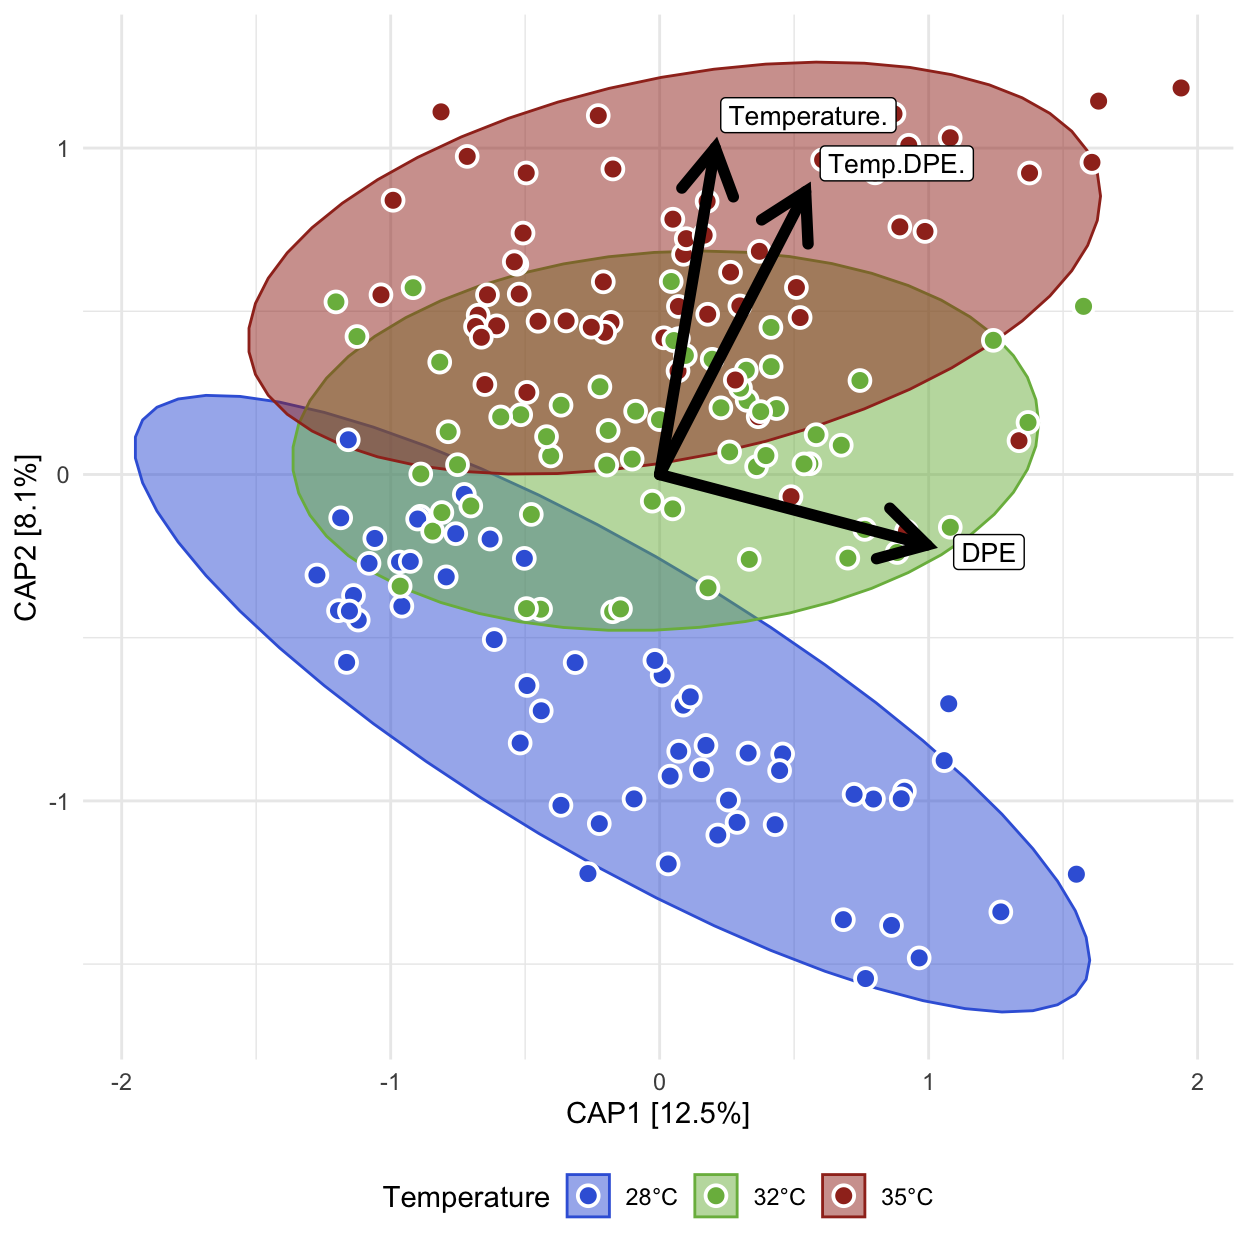
\includegraphics[keepaspectratio]{Results_Overview_files/figure-latex/plots-2D-1.pdf}}

\subparagraph{Tables}\label{tables-3}

(hide)

Click on tabs to display tables. Scroll to see additional rows.

ADONIS2

\begin{longtable}{lrrrrrr}
\caption*{
{\large ADONIS2} \\ 
{\small adonis2(Beta Distance \textasciitilde{} Temperature*DPE); Unexposed fish}
} \\ 
\toprule
term & df & SumOfSqs & R2 & statistic & p.value & sig \\ 
\midrule\addlinespace[2.5pt]
\multicolumn{7}{l}{bray} \\ 
\midrule\addlinespace[2.5pt]
Temperature & $2.000$ & $2.294$ & $0.133$ & $16.443$ & $0.001$ & *** \\ 
DPE & $1.000$ & $2.531$ & $0.147$ & $36.284$ & $0.001$ & *** \\ 
Temperature:DPE & $2.000$ & $0.896$ & $0.052$ & $6.425$ & $0.001$ & *** \\ 
Residual & $165.000$ & $11.509$ & $0.668$ & NA & NA & NA \\ 
Total & $170.000$ & $17.229$ & $1.000$ & NA & NA & NA \\ 
\midrule\addlinespace[2.5pt]
\multicolumn{7}{l}{canberra} \\ 
\midrule\addlinespace[2.5pt]
Temperature & $2.000$ & $3.862$ & $0.099$ & $10.667$ & $0.001$ & *** \\ 
DPE & $1.000$ & $3.655$ & $0.093$ & $20.192$ & $0.001$ & *** \\ 
Temperature:DPE & $2.000$ & $1.820$ & $0.046$ & $5.026$ & $0.001$ & *** \\ 
Residual & $165.000$ & $29.869$ & $0.762$ & NA & NA & NA \\ 
Total & $170.000$ & $39.206$ & $1.000$ & NA & NA & NA \\ 
\midrule\addlinespace[2.5pt]
\multicolumn{7}{l}{gunifrac} \\ 
\midrule\addlinespace[2.5pt]
Temperature & $2.000$ & $1.422$ & $0.102$ & $11.984$ & $0.001$ & *** \\ 
DPE & $1.000$ & $2.123$ & $0.153$ & $35.785$ & $0.001$ & *** \\ 
Temperature:DPE & $2.000$ & $0.574$ & $0.041$ & $4.840$ & $0.001$ & *** \\ 
Residual & $165.000$ & $9.788$ & $0.704$ & NA & NA & NA \\ 
Total & $170.000$ & $13.907$ & $1.000$ & NA & NA & NA \\ 
\bottomrule
\end{longtable}

Dispersion (ANOVA)

\begin{longtable}{lrrrrrr}
\caption*{
{\large ANOVA: Homogeneity of Dispersion} \\ 
{\small ANOVA(Beta Disperson \textasciitilde{} Temperature); Unexposed fish}
} \\ 
\toprule
term & df & sumsq & meansq & statistic & p.value & sig \\ 
\midrule\addlinespace[2.5pt]
\multicolumn{7}{l}{bray} \\ 
\midrule\addlinespace[2.5pt]
Temp.DPE & $14.000$ & $0.290$ & $0.021$ & $2.348$ & $0.006$ & ** \\ 
Residual & $156.000$ & $1.376$ & $0.009$ & NA & NA & NA \\ 
\midrule\addlinespace[2.5pt]
\multicolumn{7}{l}{canberra} \\ 
\midrule\addlinespace[2.5pt]
Temp.DPE & $14.000$ & $0.250$ & $0.018$ & $3.344$ & <0.001 & *** \\ 
Residual & $156.000$ & $0.831$ & $0.005$ & NA & NA & NA \\ 
\midrule\addlinespace[2.5pt]
\multicolumn{7}{l}{gunifrac} \\ 
\midrule\addlinespace[2.5pt]
Temp.DPE & $14.000$ & $0.249$ & $0.018$ & $2.986$ & <0.001 & *** \\ 
Residual & $156.000$ & $0.929$ & $0.006$ & NA & NA & NA \\ 
\bottomrule
\end{longtable}

Dispersion (Tukey)

\begin{longtable}{llllrrrrl}
\caption*{
{\large Tukey: Homogeneity of Dispersion} \\ 
{\small Tukey(Beta Disperson \textasciitilde{} Temperature*DPE); Unexposed fish}
} \\ 
\toprule
.y. & term & group1 & group2 & estimate & conf.low & conf.high & adj.p.value & sig \\ 
\midrule\addlinespace[2.5pt]
\multicolumn{9}{l}{bray} \\ 
\midrule\addlinespace[2.5pt]
Distance & Temp.DPE & 28°C\_\_14DPE & 28°C\_\_0DPE & $0.024$ & $-0.112$ & $0.159$ & $\geq$0.25 & ns \\ 
Distance & Temp.DPE & 28°C\_\_21DPE & 28°C\_\_0DPE & $0.052$ & $-0.074$ & $0.177$ & $\geq$0.25 & ns \\ 
Distance & Temp.DPE & 28°C\_\_28DPE & 28°C\_\_0DPE & $0.007$ & $-0.118$ & $0.133$ & $\geq$0.25 & ns \\ 
Distance & Temp.DPE & 28°C\_\_42DPE & 28°C\_\_0DPE & $-0.017$ & $-0.147$ & $0.113$ & $\geq$0.25 & ns \\ 
Distance & Temp.DPE & 32°C\_\_0DPE & 28°C\_\_0DPE & $0.097$ & $-0.005$ & $0.199$ & $0.085$ & ns \\ 
Distance & Temp.DPE & 32°C\_\_14DPE & 28°C\_\_0DPE & $0.041$ & $-0.085$ & $0.166$ & $\geq$0.25 & ns \\ 
Distance & Temp.DPE & 32°C\_\_21DPE & 28°C\_\_0DPE & $-0.018$ & $-0.143$ & $0.108$ & $\geq$0.25 & ns \\ 
Distance & Temp.DPE & 32°C\_\_28DPE & 28°C\_\_0DPE & $0.028$ & $-0.102$ & $0.158$ & $\geq$0.25 & ns \\ 
Distance & Temp.DPE & 32°C\_\_42DPE & 28°C\_\_0DPE & $0.017$ & $-0.108$ & $0.142$ & $\geq$0.25 & ns \\ 
Distance & Temp.DPE & 35°C\_\_0DPE & 28°C\_\_0DPE & $0.044$ & $-0.058$ & $0.146$ & $\geq$0.25 & ns \\ 
Distance & Temp.DPE & 35°C\_\_14DPE & 28°C\_\_0DPE & $0.004$ & $-0.126$ & $0.134$ & $\geq$0.25 & ns \\ 
Distance & Temp.DPE & 35°C\_\_21DPE & 28°C\_\_0DPE & $-0.004$ & $-0.134$ & $0.126$ & $\geq$0.25 & ns \\ 
Distance & Temp.DPE & 35°C\_\_28DPE & 28°C\_\_0DPE & $0.033$ & $-0.097$ & $0.162$ & $\geq$0.25 & ns \\ 
Distance & Temp.DPE & 35°C\_\_42DPE & 28°C\_\_0DPE & $0.146$ & $0.011$ & $0.282$ & $0.021$ & * \\ 
Distance & Temp.DPE & 28°C\_\_21DPE & 28°C\_\_14DPE & $0.028$ & $-0.126$ & $0.181$ & $\geq$0.25 & ns \\ 
Distance & Temp.DPE & 28°C\_\_28DPE & 28°C\_\_14DPE & $-0.016$ & $-0.170$ & $0.137$ & $\geq$0.25 & ns \\ 
Distance & Temp.DPE & 28°C\_\_42DPE & 28°C\_\_14DPE & $-0.040$ & $-0.198$ & $0.117$ & $\geq$0.25 & ns \\ 
Distance & Temp.DPE & 32°C\_\_0DPE & 28°C\_\_14DPE & $0.073$ & $-0.062$ & $0.209$ & $\geq$0.25 & ns \\ 
Distance & Temp.DPE & 32°C\_\_14DPE & 28°C\_\_14DPE & $0.017$ & $-0.136$ & $0.171$ & $\geq$0.25 & ns \\ 
Distance & Temp.DPE & 32°C\_\_21DPE & 28°C\_\_14DPE & $-0.041$ & $-0.195$ & $0.112$ & $\geq$0.25 & ns \\ 
Distance & Temp.DPE & 32°C\_\_28DPE & 28°C\_\_14DPE & $0.005$ & $-0.153$ & $0.162$ & $\geq$0.25 & ns \\ 
Distance & Temp.DPE & 32°C\_\_42DPE & 28°C\_\_14DPE & $-0.006$ & $-0.160$ & $0.147$ & $\geq$0.25 & ns \\ 
Distance & Temp.DPE & 35°C\_\_0DPE & 28°C\_\_14DPE & $0.020$ & $-0.115$ & $0.156$ & $\geq$0.25 & ns \\ 
Distance & Temp.DPE & 35°C\_\_14DPE & 28°C\_\_14DPE & $-0.019$ & $-0.176$ & $0.138$ & $\geq$0.25 & ns \\ 
Distance & Temp.DPE & 35°C\_\_21DPE & 28°C\_\_14DPE & $-0.028$ & $-0.185$ & $0.129$ & $\geq$0.25 & ns \\ 
Distance & Temp.DPE & 35°C\_\_28DPE & 28°C\_\_14DPE & $0.009$ & $-0.148$ & $0.166$ & $\geq$0.25 & ns \\ 
Distance & Temp.DPE & 35°C\_\_42DPE & 28°C\_\_14DPE & $0.123$ & $-0.039$ & $0.284$ & $\geq$0.25 & ns \\ 
Distance & Temp.DPE & 28°C\_\_28DPE & 28°C\_\_21DPE & $-0.044$ & $-0.189$ & $0.101$ & $\geq$0.25 & ns \\ 
Distance & Temp.DPE & 28°C\_\_42DPE & 28°C\_\_21DPE & $-0.068$ & $-0.217$ & $0.081$ & $\geq$0.25 & ns \\ 
Distance & Temp.DPE & 32°C\_\_0DPE & 28°C\_\_21DPE & $0.045$ & $-0.080$ & $0.171$ & $\geq$0.25 & ns \\ 
Distance & Temp.DPE & 32°C\_\_14DPE & 28°C\_\_21DPE & $-0.011$ & $-0.156$ & $0.134$ & $\geq$0.25 & ns \\ 
Distance & Temp.DPE & 32°C\_\_21DPE & 28°C\_\_21DPE & $-0.069$ & $-0.214$ & $0.076$ & $\geq$0.25 & ns \\ 
Distance & Temp.DPE & 32°C\_\_28DPE & 28°C\_\_21DPE & $-0.023$ & $-0.172$ & $0.125$ & $\geq$0.25 & ns \\ 
Distance & Temp.DPE & 32°C\_\_42DPE & 28°C\_\_21DPE & $-0.034$ & $-0.179$ & $0.110$ & $\geq$0.25 & ns \\ 
Distance & Temp.DPE & 35°C\_\_0DPE & 28°C\_\_21DPE & $-0.008$ & $-0.133$ & $0.118$ & $\geq$0.25 & ns \\ 
Distance & Temp.DPE & 35°C\_\_14DPE & 28°C\_\_21DPE & $-0.047$ & $-0.196$ & $0.102$ & $\geq$0.25 & ns \\ 
Distance & Temp.DPE & 35°C\_\_21DPE & 28°C\_\_21DPE & $-0.056$ & $-0.205$ & $0.093$ & $\geq$0.25 & ns \\ 
Distance & Temp.DPE & 35°C\_\_28DPE & 28°C\_\_21DPE & $-0.019$ & $-0.168$ & $0.130$ & $\geq$0.25 & ns \\ 
Distance & Temp.DPE & 35°C\_\_42DPE & 28°C\_\_21DPE & $0.095$ & $-0.059$ & $0.248$ & $\geq$0.25 & ns \\ 
Distance & Temp.DPE & 28°C\_\_42DPE & 28°C\_\_28DPE & $-0.024$ & $-0.173$ & $0.125$ & $\geq$0.25 & ns \\ 
Distance & Temp.DPE & 32°C\_\_0DPE & 28°C\_\_28DPE & $0.089$ & $-0.036$ & $0.215$ & $\geq$0.25 & ns \\ 
Distance & Temp.DPE & 32°C\_\_14DPE & 28°C\_\_28DPE & $0.033$ & $-0.111$ & $0.178$ & $\geq$0.25 & ns \\ 
Distance & Temp.DPE & 32°C\_\_21DPE & 28°C\_\_28DPE & $-0.025$ & $-0.170$ & $0.120$ & $\geq$0.25 & ns \\ 
Distance & Temp.DPE & 32°C\_\_28DPE & 28°C\_\_28DPE & $0.021$ & $-0.128$ & $0.169$ & $\geq$0.25 & ns \\ 
Distance & Temp.DPE & 32°C\_\_42DPE & 28°C\_\_28DPE & $0.010$ & $-0.135$ & $0.154$ & $\geq$0.25 & ns \\ 
Distance & Temp.DPE & 35°C\_\_0DPE & 28°C\_\_28DPE & $0.036$ & $-0.089$ & $0.162$ & $\geq$0.25 & ns \\ 
Distance & Temp.DPE & 35°C\_\_14DPE & 28°C\_\_28DPE & $-0.003$ & $-0.152$ & $0.146$ & $\geq$0.25 & ns \\ 
Distance & Temp.DPE & 35°C\_\_21DPE & 28°C\_\_28DPE & $-0.012$ & $-0.161$ & $0.137$ & $\geq$0.25 & ns \\ 
Distance & Temp.DPE & 35°C\_\_28DPE & 28°C\_\_28DPE & $0.025$ & $-0.124$ & $0.174$ & $\geq$0.25 & ns \\ 
Distance & Temp.DPE & 35°C\_\_42DPE & 28°C\_\_28DPE & $0.139$ & $-0.015$ & $0.292$ & $0.125$ & ns \\ 
Distance & Temp.DPE & 32°C\_\_0DPE & 28°C\_\_42DPE & $0.114$ & $-0.016$ & $0.243$ & $0.161$ & ns \\ 
Distance & Temp.DPE & 32°C\_\_14DPE & 28°C\_\_42DPE & $0.057$ & $-0.091$ & $0.206$ & $\geq$0.25 & ns \\ 
Distance & Temp.DPE & 32°C\_\_21DPE & 28°C\_\_42DPE & $-0.001$ & $-0.150$ & $0.148$ & $\geq$0.25 & ns \\ 
Distance & Temp.DPE & 32°C\_\_28DPE & 28°C\_\_42DPE & $0.045$ & $-0.108$ & $0.197$ & $\geq$0.25 & ns \\ 
Distance & Temp.DPE & 32°C\_\_42DPE & 28°C\_\_42DPE & $0.034$ & $-0.115$ & $0.183$ & $\geq$0.25 & ns \\ 
Distance & Temp.DPE & 35°C\_\_0DPE & 28°C\_\_42DPE & $0.061$ & $-0.069$ & $0.191$ & $\geq$0.25 & ns \\ 
Distance & Temp.DPE & 35°C\_\_14DPE & 28°C\_\_42DPE & $0.021$ & $-0.131$ & $0.174$ & $\geq$0.25 & ns \\ 
Distance & Temp.DPE & 35°C\_\_21DPE & 28°C\_\_42DPE & $0.012$ & $-0.140$ & $0.165$ & $\geq$0.25 & ns \\ 
Distance & Temp.DPE & 35°C\_\_28DPE & 28°C\_\_42DPE & $0.049$ & $-0.103$ & $0.202$ & $\geq$0.25 & ns \\ 
Distance & Temp.DPE & 35°C\_\_42DPE & 28°C\_\_42DPE & $0.163$ & $0.006$ & $0.320$ & $0.034$ & * \\ 
Distance & Temp.DPE & 32°C\_\_14DPE & 32°C\_\_0DPE & $-0.056$ & $-0.182$ & $0.069$ & $\geq$0.25 & ns \\ 
Distance & Temp.DPE & 32°C\_\_21DPE & 32°C\_\_0DPE & $-0.114$ & $-0.240$ & $0.011$ & $0.115$ & ns \\ 
Distance & Temp.DPE & 32°C\_\_28DPE & 32°C\_\_0DPE & $-0.069$ & $-0.199$ & $0.061$ & $\geq$0.25 & ns \\ 
Distance & Temp.DPE & 32°C\_\_42DPE & 32°C\_\_0DPE & $-0.080$ & $-0.205$ & $0.046$ & $\geq$0.25 & ns \\ 
Distance & Temp.DPE & 35°C\_\_0DPE & 32°C\_\_0DPE & $-0.053$ & $-0.155$ & $0.049$ & $\geq$0.25 & ns \\ 
Distance & Temp.DPE & 35°C\_\_14DPE & 32°C\_\_0DPE & $-0.092$ & $-0.222$ & $0.037$ & $\geq$0.25 & ns \\ 
Distance & Temp.DPE & 35°C\_\_21DPE & 32°C\_\_0DPE & $-0.101$ & $-0.231$ & $0.029$ & $\geq$0.25 & ns \\ 
Distance & Temp.DPE & 35°C\_\_28DPE & 32°C\_\_0DPE & $-0.064$ & $-0.194$ & $0.066$ & $\geq$0.25 & ns \\ 
Distance & Temp.DPE & 35°C\_\_42DPE & 32°C\_\_0DPE & $0.049$ & $-0.086$ & $0.185$ & $\geq$0.25 & ns \\ 
Distance & Temp.DPE & 32°C\_\_21DPE & 32°C\_\_14DPE & $-0.058$ & $-0.203$ & $0.086$ & $\geq$0.25 & ns \\ 
Distance & Temp.DPE & 32°C\_\_28DPE & 32°C\_\_14DPE & $-0.013$ & $-0.161$ & $0.136$ & $\geq$0.25 & ns \\ 
Distance & Temp.DPE & 32°C\_\_42DPE & 32°C\_\_14DPE & $-0.024$ & $-0.168$ & $0.121$ & $\geq$0.25 & ns \\ 
Distance & Temp.DPE & 35°C\_\_0DPE & 32°C\_\_14DPE & $0.003$ & $-0.122$ & $0.129$ & $\geq$0.25 & ns \\ 
Distance & Temp.DPE & 35°C\_\_14DPE & 32°C\_\_14DPE & $-0.036$ & $-0.185$ & $0.112$ & $\geq$0.25 & ns \\ 
Distance & Temp.DPE & 35°C\_\_21DPE & 32°C\_\_14DPE & $-0.045$ & $-0.194$ & $0.104$ & $\geq$0.25 & ns \\ 
Distance & Temp.DPE & 35°C\_\_28DPE & 32°C\_\_14DPE & $-0.008$ & $-0.157$ & $0.141$ & $\geq$0.25 & ns \\ 
Distance & Temp.DPE & 35°C\_\_42DPE & 32°C\_\_14DPE & $0.105$ & $-0.048$ & $0.259$ & $\geq$0.25 & ns \\ 
Distance & Temp.DPE & 32°C\_\_28DPE & 32°C\_\_21DPE & $0.046$ & $-0.103$ & $0.194$ & $\geq$0.25 & ns \\ 
Distance & Temp.DPE & 32°C\_\_42DPE & 32°C\_\_21DPE & $0.035$ & $-0.110$ & $0.179$ & $\geq$0.25 & ns \\ 
Distance & Temp.DPE & 35°C\_\_0DPE & 32°C\_\_21DPE & $0.061$ & $-0.064$ & $0.187$ & $\geq$0.25 & ns \\ 
Distance & Temp.DPE & 35°C\_\_14DPE & 32°C\_\_21DPE & $0.022$ & $-0.127$ & $0.171$ & $\geq$0.25 & ns \\ 
Distance & Temp.DPE & 35°C\_\_21DPE & 32°C\_\_21DPE & $0.013$ & $-0.136$ & $0.162$ & $\geq$0.25 & ns \\ 
Distance & Temp.DPE & 35°C\_\_28DPE & 32°C\_\_21DPE & $0.050$ & $-0.099$ & $0.199$ & $\geq$0.25 & ns \\ 
Distance & Temp.DPE & 35°C\_\_42DPE & 32°C\_\_21DPE & $0.164$ & $0.010$ & $0.317$ & $0.025$ & * \\ 
Distance & Temp.DPE & 32°C\_\_42DPE & 32°C\_\_28DPE & $-0.011$ & $-0.160$ & $0.138$ & $\geq$0.25 & ns \\ 
Distance & Temp.DPE & 35°C\_\_0DPE & 32°C\_\_28DPE & $0.016$ & $-0.114$ & $0.146$ & $\geq$0.25 & ns \\ 
Distance & Temp.DPE & 35°C\_\_14DPE & 32°C\_\_28DPE & $-0.024$ & $-0.176$ & $0.129$ & $\geq$0.25 & ns \\ 
Distance & Temp.DPE & 35°C\_\_21DPE & 32°C\_\_28DPE & $-0.033$ & $-0.185$ & $0.120$ & $\geq$0.25 & ns \\ 
Distance & Temp.DPE & 35°C\_\_28DPE & 32°C\_\_28DPE & $0.004$ & $-0.148$ & $0.157$ & $\geq$0.25 & ns \\ 
Distance & Temp.DPE & 35°C\_\_42DPE & 32°C\_\_28DPE & $0.118$ & $-0.039$ & $0.275$ & $\geq$0.25 & ns \\ 
Distance & Temp.DPE & 35°C\_\_0DPE & 32°C\_\_42DPE & $0.027$ & $-0.099$ & $0.152$ & $\geq$0.25 & ns \\ 
Distance & Temp.DPE & 35°C\_\_14DPE & 32°C\_\_42DPE & $-0.013$ & $-0.161$ & $0.136$ & $\geq$0.25 & ns \\ 
Distance & Temp.DPE & 35°C\_\_21DPE & 32°C\_\_42DPE & $-0.021$ & $-0.170$ & $0.127$ & $\geq$0.25 & ns \\ 
Distance & Temp.DPE & 35°C\_\_28DPE & 32°C\_\_42DPE & $0.015$ & $-0.133$ & $0.164$ & $\geq$0.25 & ns \\ 
Distance & Temp.DPE & 35°C\_\_42DPE & 32°C\_\_42DPE & $0.129$ & $-0.024$ & $0.283$ & $0.209$ & ns \\ 
Distance & Temp.DPE & 35°C\_\_14DPE & 35°C\_\_0DPE & $-0.039$ & $-0.169$ & $0.090$ & $\geq$0.25 & ns \\ 
Distance & Temp.DPE & 35°C\_\_21DPE & 35°C\_\_0DPE & $-0.048$ & $-0.178$ & $0.082$ & $\geq$0.25 & ns \\ 
Distance & Temp.DPE & 35°C\_\_28DPE & 35°C\_\_0DPE & $-0.011$ & $-0.141$ & $0.119$ & $\geq$0.25 & ns \\ 
Distance & Temp.DPE & 35°C\_\_42DPE & 35°C\_\_0DPE & $0.102$ & $-0.033$ & $0.238$ & $\geq$0.25 & ns \\ 
Distance & Temp.DPE & 35°C\_\_21DPE & 35°C\_\_14DPE & $-0.009$ & $-0.161$ & $0.144$ & $\geq$0.25 & ns \\ 
Distance & Temp.DPE & 35°C\_\_28DPE & 35°C\_\_14DPE & $0.028$ & $-0.124$ & $0.181$ & $\geq$0.25 & ns \\ 
Distance & Temp.DPE & 35°C\_\_42DPE & 35°C\_\_14DPE & $0.142$ & $-0.016$ & $0.299$ & $0.127$ & ns \\ 
Distance & Temp.DPE & 35°C\_\_28DPE & 35°C\_\_21DPE & $0.037$ & $-0.116$ & $0.190$ & $\geq$0.25 & ns \\ 
Distance & Temp.DPE & 35°C\_\_42DPE & 35°C\_\_21DPE & $0.151$ & $-0.007$ & $0.308$ & $0.076$ & ns \\ 
Distance & Temp.DPE & 35°C\_\_42DPE & 35°C\_\_28DPE & $0.114$ & $-0.044$ & $0.271$ & $\geq$0.25 & ns \\ 
\midrule\addlinespace[2.5pt]
\multicolumn{9}{l}{canberra} \\ 
\midrule\addlinespace[2.5pt]
Distance & Temp.DPE & 28°C\_\_14DPE & 28°C\_\_0DPE & $-0.033$ & $-0.138$ & $0.072$ & $\geq$0.25 & ns \\ 
Distance & Temp.DPE & 28°C\_\_21DPE & 28°C\_\_0DPE & $-0.005$ & $-0.103$ & $0.092$ & $\geq$0.25 & ns \\ 
Distance & Temp.DPE & 28°C\_\_28DPE & 28°C\_\_0DPE & $-0.074$ & $-0.171$ & $0.024$ & $\geq$0.25 & ns \\ 
Distance & Temp.DPE & 28°C\_\_42DPE & 28°C\_\_0DPE & $-0.069$ & $-0.170$ & $0.032$ & $\geq$0.25 & ns \\ 
Distance & Temp.DPE & 32°C\_\_0DPE & 28°C\_\_0DPE & $0.035$ & $-0.045$ & $0.115$ & $\geq$0.25 & ns \\ 
Distance & Temp.DPE & 32°C\_\_14DPE & 28°C\_\_0DPE & $-0.021$ & $-0.119$ & $0.076$ & $\geq$0.25 & ns \\ 
Distance & Temp.DPE & 32°C\_\_21DPE & 28°C\_\_0DPE & $-0.070$ & $-0.167$ & $0.028$ & $\geq$0.25 & ns \\ 
Distance & Temp.DPE & 32°C\_\_28DPE & 28°C\_\_0DPE & $-0.056$ & $-0.157$ & $0.045$ & $\geq$0.25 & ns \\ 
Distance & Temp.DPE & 32°C\_\_42DPE & 28°C\_\_0DPE & $-0.068$ & $-0.165$ & $0.030$ & $\geq$0.25 & ns \\ 
Distance & Temp.DPE & 35°C\_\_0DPE & 28°C\_\_0DPE & $0.008$ & $-0.071$ & $0.088$ & $\geq$0.25 & ns \\ 
Distance & Temp.DPE & 35°C\_\_14DPE & 28°C\_\_0DPE & $-0.041$ & $-0.142$ & $0.060$ & $\geq$0.25 & ns \\ 
Distance & Temp.DPE & 35°C\_\_21DPE & 28°C\_\_0DPE & $-0.047$ & $-0.148$ & $0.054$ & $\geq$0.25 & ns \\ 
Distance & Temp.DPE & 35°C\_\_28DPE & 28°C\_\_0DPE & $-0.052$ & $-0.153$ & $0.049$ & $\geq$0.25 & ns \\ 
Distance & Temp.DPE & 35°C\_\_42DPE & 28°C\_\_0DPE & $0.045$ & $-0.061$ & $0.150$ & $\geq$0.25 & ns \\ 
Distance & Temp.DPE & 28°C\_\_21DPE & 28°C\_\_14DPE & $0.028$ & $-0.091$ & $0.147$ & $\geq$0.25 & ns \\ 
Distance & Temp.DPE & 28°C\_\_28DPE & 28°C\_\_14DPE & $-0.040$ & $-0.160$ & $0.079$ & $\geq$0.25 & ns \\ 
Distance & Temp.DPE & 28°C\_\_42DPE & 28°C\_\_14DPE & $-0.035$ & $-0.158$ & $0.087$ & $\geq$0.25 & ns \\ 
Distance & Temp.DPE & 32°C\_\_0DPE & 28°C\_\_14DPE & $0.068$ & $-0.037$ & $0.174$ & $\geq$0.25 & ns \\ 
Distance & Temp.DPE & 32°C\_\_14DPE & 28°C\_\_14DPE & $0.012$ & $-0.107$ & $0.131$ & $\geq$0.25 & ns \\ 
Distance & Temp.DPE & 32°C\_\_21DPE & 28°C\_\_14DPE & $-0.037$ & $-0.156$ & $0.083$ & $\geq$0.25 & ns \\ 
Distance & Temp.DPE & 32°C\_\_28DPE & 28°C\_\_14DPE & $-0.023$ & $-0.145$ & $0.099$ & $\geq$0.25 & ns \\ 
Distance & Temp.DPE & 32°C\_\_42DPE & 28°C\_\_14DPE & $-0.034$ & $-0.154$ & $0.085$ & $\geq$0.25 & ns \\ 
Distance & Temp.DPE & 35°C\_\_0DPE & 28°C\_\_14DPE & $0.042$ & $-0.064$ & $0.147$ & $\geq$0.25 & ns \\ 
Distance & Temp.DPE & 35°C\_\_14DPE & 28°C\_\_14DPE & $-0.008$ & $-0.130$ & $0.115$ & $\geq$0.25 & ns \\ 
Distance & Temp.DPE & 35°C\_\_21DPE & 28°C\_\_14DPE & $-0.013$ & $-0.136$ & $0.109$ & $\geq$0.25 & ns \\ 
Distance & Temp.DPE & 35°C\_\_28DPE & 28°C\_\_14DPE & $-0.019$ & $-0.141$ & $0.103$ & $\geq$0.25 & ns \\ 
Distance & Temp.DPE & 35°C\_\_42DPE & 28°C\_\_14DPE & $0.078$ & $-0.048$ & $0.204$ & $\geq$0.25 & ns \\ 
Distance & Temp.DPE & 28°C\_\_28DPE & 28°C\_\_21DPE & $-0.068$ & $-0.181$ & $0.044$ & $\geq$0.25 & ns \\ 
Distance & Temp.DPE & 28°C\_\_42DPE & 28°C\_\_21DPE & $-0.063$ & $-0.179$ & $0.052$ & $\geq$0.25 & ns \\ 
Distance & Temp.DPE & 32°C\_\_0DPE & 28°C\_\_21DPE & $0.040$ & $-0.057$ & $0.138$ & $\geq$0.25 & ns \\ 
Distance & Temp.DPE & 32°C\_\_14DPE & 28°C\_\_21DPE & $-0.016$ & $-0.128$ & $0.097$ & $\geq$0.25 & ns \\ 
Distance & Temp.DPE & 32°C\_\_21DPE & 28°C\_\_21DPE & $-0.065$ & $-0.177$ & $0.048$ & $\geq$0.25 & ns \\ 
Distance & Temp.DPE & 32°C\_\_28DPE & 28°C\_\_21DPE & $-0.051$ & $-0.167$ & $0.065$ & $\geq$0.25 & ns \\ 
Distance & Temp.DPE & 32°C\_\_42DPE & 28°C\_\_21DPE & $-0.062$ & $-0.175$ & $0.050$ & $\geq$0.25 & ns \\ 
Distance & Temp.DPE & 35°C\_\_0DPE & 28°C\_\_21DPE & $0.014$ & $-0.084$ & $0.111$ & $\geq$0.25 & ns \\ 
Distance & Temp.DPE & 35°C\_\_14DPE & 28°C\_\_21DPE & $-0.036$ & $-0.151$ & $0.080$ & $\geq$0.25 & ns \\ 
Distance & Temp.DPE & 35°C\_\_21DPE & 28°C\_\_21DPE & $-0.041$ & $-0.157$ & $0.074$ & $\geq$0.25 & ns \\ 
Distance & Temp.DPE & 35°C\_\_28DPE & 28°C\_\_21DPE & $-0.047$ & $-0.162$ & $0.069$ & $\geq$0.25 & ns \\ 
Distance & Temp.DPE & 35°C\_\_42DPE & 28°C\_\_21DPE & $0.050$ & $-0.070$ & $0.169$ & $\geq$0.25 & ns \\ 
Distance & Temp.DPE & 28°C\_\_42DPE & 28°C\_\_28DPE & $0.005$ & $-0.110$ & $0.121$ & $\geq$0.25 & ns \\ 
Distance & Temp.DPE & 32°C\_\_0DPE & 28°C\_\_28DPE & $0.109$ & $0.011$ & $0.206$ & $0.014$ & * \\ 
Distance & Temp.DPE & 32°C\_\_14DPE & 28°C\_\_28DPE & $0.052$ & $-0.060$ & $0.165$ & $\geq$0.25 & ns \\ 
Distance & Temp.DPE & 32°C\_\_21DPE & 28°C\_\_28DPE & $0.004$ & $-0.109$ & $0.116$ & $\geq$0.25 & ns \\ 
Distance & Temp.DPE & 32°C\_\_28DPE & 28°C\_\_28DPE & $0.017$ & $-0.098$ & $0.133$ & $\geq$0.25 & ns \\ 
Distance & Temp.DPE & 32°C\_\_42DPE & 28°C\_\_28DPE & $0.006$ & $-0.106$ & $0.119$ & $\geq$0.25 & ns \\ 
Distance & Temp.DPE & 35°C\_\_0DPE & 28°C\_\_28DPE & $0.082$ & $-0.015$ & $0.180$ & $0.206$ & ns \\ 
Distance & Temp.DPE & 35°C\_\_14DPE & 28°C\_\_28DPE & $0.033$ & $-0.083$ & $0.148$ & $\geq$0.25 & ns \\ 
Distance & Temp.DPE & 35°C\_\_21DPE & 28°C\_\_28DPE & $0.027$ & $-0.088$ & $0.143$ & $\geq$0.25 & ns \\ 
Distance & Temp.DPE & 35°C\_\_28DPE & 28°C\_\_28DPE & $0.021$ & $-0.094$ & $0.137$ & $\geq$0.25 & ns \\ 
Distance & Temp.DPE & 35°C\_\_42DPE & 28°C\_\_28DPE & $0.118$ & $-0.001$ & $0.237$ & $0.055$ & ns \\ 
Distance & Temp.DPE & 32°C\_\_0DPE & 28°C\_\_42DPE & $0.104$ & $0.003$ & $0.205$ & $0.038$ & * \\ 
Distance & Temp.DPE & 32°C\_\_14DPE & 28°C\_\_42DPE & $0.047$ & $-0.068$ & $0.163$ & $\geq$0.25 & ns \\ 
Distance & Temp.DPE & 32°C\_\_21DPE & 28°C\_\_42DPE & $-0.001$ & $-0.117$ & $0.114$ & $\geq$0.25 & ns \\ 
Distance & Temp.DPE & 32°C\_\_28DPE & 28°C\_\_42DPE & $0.012$ & $-0.106$ & $0.131$ & $\geq$0.25 & ns \\ 
Distance & Temp.DPE & 32°C\_\_42DPE & 28°C\_\_42DPE & $0.001$ & $-0.115$ & $0.117$ & $\geq$0.25 & ns \\ 
Distance & Temp.DPE & 35°C\_\_0DPE & 28°C\_\_42DPE & $0.077$ & $-0.024$ & $0.178$ & $\geq$0.25 & ns \\ 
Distance & Temp.DPE & 35°C\_\_14DPE & 28°C\_\_42DPE & $0.028$ & $-0.091$ & $0.146$ & $\geq$0.25 & ns \\ 
Distance & Temp.DPE & 35°C\_\_21DPE & 28°C\_\_42DPE & $0.022$ & $-0.097$ & $0.141$ & $\geq$0.25 & ns \\ 
Distance & Temp.DPE & 35°C\_\_28DPE & 28°C\_\_42DPE & $0.016$ & $-0.102$ & $0.135$ & $\geq$0.25 & ns \\ 
Distance & Temp.DPE & 35°C\_\_42DPE & 28°C\_\_42DPE & $0.113$ & $-0.009$ & $0.235$ & $0.104$ & ns \\ 
Distance & Temp.DPE & 32°C\_\_14DPE & 32°C\_\_0DPE & $-0.056$ & $-0.154$ & $0.041$ & $\geq$0.25 & ns \\ 
Distance & Temp.DPE & 32°C\_\_21DPE & 32°C\_\_0DPE & $-0.105$ & $-0.202$ & $-0.007$ & $0.022$ & * \\ 
Distance & Temp.DPE & 32°C\_\_28DPE & 32°C\_\_0DPE & $-0.091$ & $-0.192$ & $0.010$ & $0.125$ & ns \\ 
Distance & Temp.DPE & 32°C\_\_42DPE & 32°C\_\_0DPE & $-0.103$ & $-0.200$ & $-0.005$ & $0.029$ & * \\ 
Distance & Temp.DPE & 35°C\_\_0DPE & 32°C\_\_0DPE & $-0.027$ & $-0.106$ & $0.053$ & $\geq$0.25 & ns \\ 
Distance & Temp.DPE & 35°C\_\_14DPE & 32°C\_\_0DPE & $-0.076$ & $-0.177$ & $0.025$ & $\geq$0.25 & ns \\ 
Distance & Temp.DPE & 35°C\_\_21DPE & 32°C\_\_0DPE & $-0.082$ & $-0.183$ & $0.019$ & $\geq$0.25 & ns \\ 
Distance & Temp.DPE & 35°C\_\_28DPE & 32°C\_\_0DPE & $-0.087$ & $-0.188$ & $0.014$ & $0.175$ & ns \\ 
Distance & Temp.DPE & 35°C\_\_42DPE & 32°C\_\_0DPE & $0.009$ & $-0.096$ & $0.115$ & $\geq$0.25 & ns \\ 
Distance & Temp.DPE & 32°C\_\_21DPE & 32°C\_\_14DPE & $-0.049$ & $-0.161$ & $0.064$ & $\geq$0.25 & ns \\ 
Distance & Temp.DPE & 32°C\_\_28DPE & 32°C\_\_14DPE & $-0.035$ & $-0.151$ & $0.081$ & $\geq$0.25 & ns \\ 
Distance & Temp.DPE & 32°C\_\_42DPE & 32°C\_\_14DPE & $-0.046$ & $-0.159$ & $0.066$ & $\geq$0.25 & ns \\ 
Distance & Temp.DPE & 35°C\_\_0DPE & 32°C\_\_14DPE & $0.030$ & $-0.068$ & $0.127$ & $\geq$0.25 & ns \\ 
Distance & Temp.DPE & 35°C\_\_14DPE & 32°C\_\_14DPE & $-0.020$ & $-0.135$ & $0.096$ & $\geq$0.25 & ns \\ 
Distance & Temp.DPE & 35°C\_\_21DPE & 32°C\_\_14DPE & $-0.025$ & $-0.141$ & $0.090$ & $\geq$0.25 & ns \\ 
Distance & Temp.DPE & 35°C\_\_28DPE & 32°C\_\_14DPE & $-0.031$ & $-0.147$ & $0.085$ & $\geq$0.25 & ns \\ 
Distance & Temp.DPE & 35°C\_\_42DPE & 32°C\_\_14DPE & $0.066$ & $-0.054$ & $0.185$ & $\geq$0.25 & ns \\ 
Distance & Temp.DPE & 32°C\_\_28DPE & 32°C\_\_21DPE & $0.014$ & $-0.102$ & $0.129$ & $\geq$0.25 & ns \\ 
Distance & Temp.DPE & 32°C\_\_42DPE & 32°C\_\_21DPE & $0.002$ & $-0.110$ & $0.115$ & $\geq$0.25 & ns \\ 
Distance & Temp.DPE & 35°C\_\_0DPE & 32°C\_\_21DPE & $0.078$ & $-0.019$ & $0.176$ & $\geq$0.25 & ns \\ 
Distance & Temp.DPE & 35°C\_\_14DPE & 32°C\_\_21DPE & $0.029$ & $-0.087$ & $0.145$ & $\geq$0.25 & ns \\ 
Distance & Temp.DPE & 35°C\_\_21DPE & 32°C\_\_21DPE & $0.023$ & $-0.092$ & $0.139$ & $\geq$0.25 & ns \\ 
Distance & Temp.DPE & 35°C\_\_28DPE & 32°C\_\_21DPE & $0.018$ & $-0.098$ & $0.133$ & $\geq$0.25 & ns \\ 
Distance & Temp.DPE & 35°C\_\_42DPE & 32°C\_\_21DPE & $0.114$ & $-0.005$ & $0.234$ & $0.076$ & ns \\ 
Distance & Temp.DPE & 32°C\_\_42DPE & 32°C\_\_28DPE & $-0.011$ & $-0.127$ & $0.104$ & $\geq$0.25 & ns \\ 
Distance & Temp.DPE & 35°C\_\_0DPE & 32°C\_\_28DPE & $0.065$ & $-0.036$ & $0.166$ & $\geq$0.25 & ns \\ 
Distance & Temp.DPE & 35°C\_\_14DPE & 32°C\_\_28DPE & $0.015$ & $-0.103$ & $0.134$ & $\geq$0.25 & ns \\ 
Distance & Temp.DPE & 35°C\_\_21DPE & 32°C\_\_28DPE & $0.010$ & $-0.109$ & $0.128$ & $\geq$0.25 & ns \\ 
Distance & Temp.DPE & 35°C\_\_28DPE & 32°C\_\_28DPE & $0.004$ & $-0.115$ & $0.123$ & $\geq$0.25 & ns \\ 
Distance & Temp.DPE & 35°C\_\_42DPE & 32°C\_\_28DPE & $0.101$ & $-0.022$ & $0.223$ & $0.237$ & ns \\ 
Distance & Temp.DPE & 35°C\_\_0DPE & 32°C\_\_42DPE & $0.076$ & $-0.021$ & $0.173$ & $\geq$0.25 & ns \\ 
Distance & Temp.DPE & 35°C\_\_14DPE & 32°C\_\_42DPE & $0.027$ & $-0.089$ & $0.142$ & $\geq$0.25 & ns \\ 
Distance & Temp.DPE & 35°C\_\_21DPE & 32°C\_\_42DPE & $0.021$ & $-0.095$ & $0.137$ & $\geq$0.25 & ns \\ 
Distance & Temp.DPE & 35°C\_\_28DPE & 32°C\_\_42DPE & $0.015$ & $-0.100$ & $0.131$ & $\geq$0.25 & ns \\ 
Distance & Temp.DPE & 35°C\_\_42DPE & 32°C\_\_42DPE & $0.112$ & $-0.007$ & $0.231$ & $0.091$ & ns \\ 
Distance & Temp.DPE & 35°C\_\_14DPE & 35°C\_\_0DPE & $-0.049$ & $-0.150$ & $0.052$ & $\geq$0.25 & ns \\ 
Distance & Temp.DPE & 35°C\_\_21DPE & 35°C\_\_0DPE & $-0.055$ & $-0.156$ & $0.046$ & $\geq$0.25 & ns \\ 
Distance & Temp.DPE & 35°C\_\_28DPE & 35°C\_\_0DPE & $-0.061$ & $-0.162$ & $0.040$ & $\geq$0.25 & ns \\ 
Distance & Temp.DPE & 35°C\_\_42DPE & 35°C\_\_0DPE & $0.036$ & $-0.069$ & $0.141$ & $\geq$0.25 & ns \\ 
Distance & Temp.DPE & 35°C\_\_21DPE & 35°C\_\_14DPE & $-0.006$ & $-0.124$ & $0.113$ & $\geq$0.25 & ns \\ 
Distance & Temp.DPE & 35°C\_\_28DPE & 35°C\_\_14DPE & $-0.011$ & $-0.130$ & $0.107$ & $\geq$0.25 & ns \\ 
Distance & Temp.DPE & 35°C\_\_42DPE & 35°C\_\_14DPE & $0.085$ & $-0.037$ & $0.208$ & $\geq$0.25 & ns \\ 
Distance & Temp.DPE & 35°C\_\_28DPE & 35°C\_\_21DPE & $-0.006$ & $-0.124$ & $0.113$ & $\geq$0.25 & ns \\ 
Distance & Temp.DPE & 35°C\_\_42DPE & 35°C\_\_21DPE & $0.091$ & $-0.031$ & $0.213$ & $\geq$0.25 & ns \\ 
Distance & Temp.DPE & 35°C\_\_42DPE & 35°C\_\_28DPE & $0.097$ & $-0.026$ & $0.219$ & $\geq$0.25 & ns \\ 
\midrule\addlinespace[2.5pt]
\multicolumn{9}{l}{gunifrac} \\ 
\midrule\addlinespace[2.5pt]
Distance & Temp.DPE & 28°C\_\_14DPE & 28°C\_\_0DPE & $-0.005$ & $-0.116$ & $0.107$ & $\geq$0.25 & ns \\ 
Distance & Temp.DPE & 28°C\_\_21DPE & 28°C\_\_0DPE & $0.038$ & $-0.065$ & $0.141$ & $\geq$0.25 & ns \\ 
Distance & Temp.DPE & 28°C\_\_28DPE & 28°C\_\_0DPE & $-0.010$ & $-0.113$ & $0.093$ & $\geq$0.25 & ns \\ 
Distance & Temp.DPE & 28°C\_\_42DPE & 28°C\_\_0DPE & $-0.033$ & $-0.140$ & $0.073$ & $\geq$0.25 & ns \\ 
Distance & Temp.DPE & 32°C\_\_0DPE & 28°C\_\_0DPE & $0.067$ & $-0.017$ & $0.151$ & $\geq$0.25 & ns \\ 
Distance & Temp.DPE & 32°C\_\_14DPE & 28°C\_\_0DPE & $0.018$ & $-0.085$ & $0.121$ & $\geq$0.25 & ns \\ 
Distance & Temp.DPE & 32°C\_\_21DPE & 28°C\_\_0DPE & $-0.023$ & $-0.126$ & $0.080$ & $\geq$0.25 & ns \\ 
Distance & Temp.DPE & 32°C\_\_28DPE & 28°C\_\_0DPE & $-0.014$ & $-0.121$ & $0.093$ & $\geq$0.25 & ns \\ 
Distance & Temp.DPE & 32°C\_\_42DPE & 28°C\_\_0DPE & $-0.026$ & $-0.129$ & $0.077$ & $\geq$0.25 & ns \\ 
Distance & Temp.DPE & 35°C\_\_0DPE & 28°C\_\_0DPE & $0.029$ & $-0.055$ & $0.113$ & $\geq$0.25 & ns \\ 
Distance & Temp.DPE & 35°C\_\_14DPE & 28°C\_\_0DPE & $-0.015$ & $-0.122$ & $0.092$ & $\geq$0.25 & ns \\ 
Distance & Temp.DPE & 35°C\_\_21DPE & 28°C\_\_0DPE & $-0.020$ & $-0.127$ & $0.087$ & $\geq$0.25 & ns \\ 
Distance & Temp.DPE & 35°C\_\_28DPE & 28°C\_\_0DPE & $-0.065$ & $-0.171$ & $0.042$ & $\geq$0.25 & ns \\ 
Distance & Temp.DPE & 35°C\_\_42DPE & 28°C\_\_0DPE & $0.091$ & $-0.020$ & $0.202$ & $0.245$ & ns \\ 
Distance & Temp.DPE & 28°C\_\_21DPE & 28°C\_\_14DPE & $0.042$ & $-0.084$ & $0.168$ & $\geq$0.25 & ns \\ 
Distance & Temp.DPE & 28°C\_\_28DPE & 28°C\_\_14DPE & $-0.005$ & $-0.131$ & $0.121$ & $\geq$0.25 & ns \\ 
Distance & Temp.DPE & 28°C\_\_42DPE & 28°C\_\_14DPE & $-0.029$ & $-0.158$ & $0.100$ & $\geq$0.25 & ns \\ 
Distance & Temp.DPE & 32°C\_\_0DPE & 28°C\_\_14DPE & $0.072$ & $-0.040$ & $0.183$ & $\geq$0.25 & ns \\ 
Distance & Temp.DPE & 32°C\_\_14DPE & 28°C\_\_14DPE & $0.022$ & $-0.104$ & $0.148$ & $\geq$0.25 & ns \\ 
Distance & Temp.DPE & 32°C\_\_21DPE & 28°C\_\_14DPE & $-0.019$ & $-0.145$ & $0.107$ & $\geq$0.25 & ns \\ 
Distance & Temp.DPE & 32°C\_\_28DPE & 28°C\_\_14DPE & $-0.009$ & $-0.138$ & $0.120$ & $\geq$0.25 & ns \\ 
Distance & Temp.DPE & 32°C\_\_42DPE & 28°C\_\_14DPE & $-0.021$ & $-0.147$ & $0.105$ & $\geq$0.25 & ns \\ 
Distance & Temp.DPE & 35°C\_\_0DPE & 28°C\_\_14DPE & $0.033$ & $-0.078$ & $0.145$ & $\geq$0.25 & ns \\ 
Distance & Temp.DPE & 35°C\_\_14DPE & 28°C\_\_14DPE & $-0.010$ & $-0.139$ & $0.119$ & $\geq$0.25 & ns \\ 
Distance & Temp.DPE & 35°C\_\_21DPE & 28°C\_\_14DPE & $-0.015$ & $-0.145$ & $0.114$ & $\geq$0.25 & ns \\ 
Distance & Temp.DPE & 35°C\_\_28DPE & 28°C\_\_14DPE & $-0.060$ & $-0.189$ & $0.069$ & $\geq$0.25 & ns \\ 
Distance & Temp.DPE & 35°C\_\_42DPE & 28°C\_\_14DPE & $0.096$ & $-0.037$ & $0.229$ & $\geq$0.25 & ns \\ 
Distance & Temp.DPE & 28°C\_\_28DPE & 28°C\_\_21DPE & $-0.047$ & $-0.166$ & $0.072$ & $\geq$0.25 & ns \\ 
Distance & Temp.DPE & 28°C\_\_42DPE & 28°C\_\_21DPE & $-0.071$ & $-0.193$ & $0.051$ & $\geq$0.25 & ns \\ 
Distance & Temp.DPE & 32°C\_\_0DPE & 28°C\_\_21DPE & $0.029$ & $-0.074$ & $0.132$ & $\geq$0.25 & ns \\ 
Distance & Temp.DPE & 32°C\_\_14DPE & 28°C\_\_21DPE & $-0.020$ & $-0.139$ & $0.099$ & $\geq$0.25 & ns \\ 
Distance & Temp.DPE & 32°C\_\_21DPE & 28°C\_\_21DPE & $-0.061$ & $-0.180$ & $0.058$ & $\geq$0.25 & ns \\ 
Distance & Temp.DPE & 32°C\_\_28DPE & 28°C\_\_21DPE & $-0.051$ & $-0.174$ & $0.071$ & $\geq$0.25 & ns \\ 
Distance & Temp.DPE & 32°C\_\_42DPE & 28°C\_\_21DPE & $-0.063$ & $-0.182$ & $0.056$ & $\geq$0.25 & ns \\ 
Distance & Temp.DPE & 35°C\_\_0DPE & 28°C\_\_21DPE & $-0.009$ & $-0.112$ & $0.094$ & $\geq$0.25 & ns \\ 
Distance & Temp.DPE & 35°C\_\_14DPE & 28°C\_\_21DPE & $-0.052$ & $-0.175$ & $0.070$ & $\geq$0.25 & ns \\ 
Distance & Temp.DPE & 35°C\_\_21DPE & 28°C\_\_21DPE & $-0.058$ & $-0.180$ & $0.065$ & $\geq$0.25 & ns \\ 
Distance & Temp.DPE & 35°C\_\_28DPE & 28°C\_\_21DPE & $-0.102$ & $-0.224$ & $0.020$ & $0.216$ & ns \\ 
Distance & Temp.DPE & 35°C\_\_42DPE & 28°C\_\_21DPE & $0.054$ & $-0.073$ & $0.180$ & $\geq$0.25 & ns \\ 
Distance & Temp.DPE & 28°C\_\_42DPE & 28°C\_\_28DPE & $-0.024$ & $-0.146$ & $0.098$ & $\geq$0.25 & ns \\ 
Distance & Temp.DPE & 32°C\_\_0DPE & 28°C\_\_28DPE & $0.077$ & $-0.026$ & $0.180$ & $\geq$0.25 & ns \\ 
Distance & Temp.DPE & 32°C\_\_14DPE & 28°C\_\_28DPE & $0.027$ & $-0.092$ & $0.146$ & $\geq$0.25 & ns \\ 
Distance & Temp.DPE & 32°C\_\_21DPE & 28°C\_\_28DPE & $-0.014$ & $-0.133$ & $0.105$ & $\geq$0.25 & ns \\ 
Distance & Temp.DPE & 32°C\_\_28DPE & 28°C\_\_28DPE & $-0.004$ & $-0.126$ & $0.118$ & $\geq$0.25 & ns \\ 
Distance & Temp.DPE & 32°C\_\_42DPE & 28°C\_\_28DPE & $-0.016$ & $-0.135$ & $0.103$ & $\geq$0.25 & ns \\ 
Distance & Temp.DPE & 35°C\_\_0DPE & 28°C\_\_28DPE & $0.038$ & $-0.065$ & $0.142$ & $\geq$0.25 & ns \\ 
Distance & Temp.DPE & 35°C\_\_14DPE & 28°C\_\_28DPE & $-0.005$ & $-0.127$ & $0.117$ & $\geq$0.25 & ns \\ 
Distance & Temp.DPE & 35°C\_\_21DPE & 28°C\_\_28DPE & $-0.010$ & $-0.132$ & $0.112$ & $\geq$0.25 & ns \\ 
Distance & Temp.DPE & 35°C\_\_28DPE & 28°C\_\_28DPE & $-0.055$ & $-0.177$ & $0.067$ & $\geq$0.25 & ns \\ 
Distance & Temp.DPE & 35°C\_\_42DPE & 28°C\_\_28DPE & $0.101$ & $-0.025$ & $0.227$ & $\geq$0.25 & ns \\ 
Distance & Temp.DPE & 32°C\_\_0DPE & 28°C\_\_42DPE & $0.100$ & $-0.006$ & $0.207$ & $0.089$ & ns \\ 
Distance & Temp.DPE & 32°C\_\_14DPE & 28°C\_\_42DPE & $0.051$ & $-0.071$ & $0.173$ & $\geq$0.25 & ns \\ 
Distance & Temp.DPE & 32°C\_\_21DPE & 28°C\_\_42DPE & $0.010$ & $-0.112$ & $0.132$ & $\geq$0.25 & ns \\ 
Distance & Temp.DPE & 32°C\_\_28DPE & 28°C\_\_42DPE & $0.020$ & $-0.106$ & $0.145$ & $\geq$0.25 & ns \\ 
Distance & Temp.DPE & 32°C\_\_42DPE & 28°C\_\_42DPE & $0.008$ & $-0.114$ & $0.130$ & $\geq$0.25 & ns \\ 
Distance & Temp.DPE & 35°C\_\_0DPE & 28°C\_\_42DPE & $0.062$ & $-0.045$ & $0.169$ & $\geq$0.25 & ns \\ 
Distance & Temp.DPE & 35°C\_\_14DPE & 28°C\_\_42DPE & $0.019$ & $-0.107$ & $0.144$ & $\geq$0.25 & ns \\ 
Distance & Temp.DPE & 35°C\_\_21DPE & 28°C\_\_42DPE & $0.014$ & $-0.112$ & $0.139$ & $\geq$0.25 & ns \\ 
Distance & Temp.DPE & 35°C\_\_28DPE & 28°C\_\_42DPE & $-0.031$ & $-0.157$ & $0.094$ & $\geq$0.25 & ns \\ 
Distance & Temp.DPE & 35°C\_\_42DPE & 28°C\_\_42DPE & $0.125$ & $-0.005$ & $0.254$ & $0.071$ & ns \\ 
Distance & Temp.DPE & 32°C\_\_14DPE & 32°C\_\_0DPE & $-0.049$ & $-0.152$ & $0.054$ & $\geq$0.25 & ns \\ 
Distance & Temp.DPE & 32°C\_\_21DPE & 32°C\_\_0DPE & $-0.090$ & $-0.193$ & $0.013$ & $0.155$ & ns \\ 
Distance & Temp.DPE & 32°C\_\_28DPE & 32°C\_\_0DPE & $-0.081$ & $-0.188$ & $0.026$ & $\geq$0.25 & ns \\ 
Distance & Temp.DPE & 32°C\_\_42DPE & 32°C\_\_0DPE & $-0.093$ & $-0.196$ & $0.010$ & $0.130$ & ns \\ 
Distance & Temp.DPE & 35°C\_\_0DPE & 32°C\_\_0DPE & $-0.038$ & $-0.122$ & $0.046$ & $\geq$0.25 & ns \\ 
Distance & Temp.DPE & 35°C\_\_14DPE & 32°C\_\_0DPE & $-0.082$ & $-0.189$ & $0.025$ & $\geq$0.25 & ns \\ 
Distance & Temp.DPE & 35°C\_\_21DPE & 32°C\_\_0DPE & $-0.087$ & $-0.194$ & $0.020$ & $\geq$0.25 & ns \\ 
Distance & Temp.DPE & 35°C\_\_28DPE & 32°C\_\_0DPE & $-0.132$ & $-0.238$ & $-0.025$ & $0.003$ & ** \\ 
Distance & Temp.DPE & 35°C\_\_42DPE & 32°C\_\_0DPE & $0.024$ & $-0.087$ & $0.135$ & $\geq$0.25 & ns \\ 
Distance & Temp.DPE & 32°C\_\_21DPE & 32°C\_\_14DPE & $-0.041$ & $-0.160$ & $0.078$ & $\geq$0.25 & ns \\ 
Distance & Temp.DPE & 32°C\_\_28DPE & 32°C\_\_14DPE & $-0.031$ & $-0.154$ & $0.091$ & $\geq$0.25 & ns \\ 
Distance & Temp.DPE & 32°C\_\_42DPE & 32°C\_\_14DPE & $-0.043$ & $-0.162$ & $0.076$ & $\geq$0.25 & ns \\ 
Distance & Temp.DPE & 35°C\_\_0DPE & 32°C\_\_14DPE & $0.011$ & $-0.092$ & $0.114$ & $\geq$0.25 & ns \\ 
Distance & Temp.DPE & 35°C\_\_14DPE & 32°C\_\_14DPE & $-0.032$ & $-0.155$ & $0.090$ & $\geq$0.25 & ns \\ 
Distance & Temp.DPE & 35°C\_\_21DPE & 32°C\_\_14DPE & $-0.037$ & $-0.160$ & $0.085$ & $\geq$0.25 & ns \\ 
Distance & Temp.DPE & 35°C\_\_28DPE & 32°C\_\_14DPE & $-0.082$ & $-0.204$ & $0.040$ & $\geq$0.25 & ns \\ 
Distance & Temp.DPE & 35°C\_\_42DPE & 32°C\_\_14DPE & $0.074$ & $-0.053$ & $0.200$ & $\geq$0.25 & ns \\ 
Distance & Temp.DPE & 32°C\_\_28DPE & 32°C\_\_21DPE & $0.010$ & $-0.113$ & $0.132$ & $\geq$0.25 & ns \\ 
Distance & Temp.DPE & 32°C\_\_42DPE & 32°C\_\_21DPE & $-0.002$ & $-0.121$ & $0.117$ & $\geq$0.25 & ns \\ 
Distance & Temp.DPE & 35°C\_\_0DPE & 32°C\_\_21DPE & $0.052$ & $-0.051$ & $0.155$ & $\geq$0.25 & ns \\ 
Distance & Temp.DPE & 35°C\_\_14DPE & 32°C\_\_21DPE & $0.009$ & $-0.114$ & $0.131$ & $\geq$0.25 & ns \\ 
Distance & Temp.DPE & 35°C\_\_21DPE & 32°C\_\_21DPE & $0.004$ & $-0.119$ & $0.126$ & $\geq$0.25 & ns \\ 
Distance & Temp.DPE & 35°C\_\_28DPE & 32°C\_\_21DPE & $-0.041$ & $-0.163$ & $0.081$ & $\geq$0.25 & ns \\ 
Distance & Temp.DPE & 35°C\_\_42DPE & 32°C\_\_21DPE & $0.115$ & $-0.011$ & $0.241$ & $0.119$ & ns \\ 
Distance & Temp.DPE & 32°C\_\_42DPE & 32°C\_\_28DPE & $-0.012$ & $-0.134$ & $0.110$ & $\geq$0.25 & ns \\ 
Distance & Temp.DPE & 35°C\_\_0DPE & 32°C\_\_28DPE & $0.043$ & $-0.064$ & $0.149$ & $\geq$0.25 & ns \\ 
Distance & Temp.DPE & 35°C\_\_14DPE & 32°C\_\_28DPE & $-0.001$ & $-0.126$ & $0.124$ & $\geq$0.25 & ns \\ 
Distance & Temp.DPE & 35°C\_\_21DPE & 32°C\_\_28DPE & $-0.006$ & $-0.132$ & $0.119$ & $\geq$0.25 & ns \\ 
Distance & Temp.DPE & 35°C\_\_28DPE & 32°C\_\_28DPE & $-0.051$ & $-0.176$ & $0.075$ & $\geq$0.25 & ns \\ 
Distance & Temp.DPE & 35°C\_\_42DPE & 32°C\_\_28DPE & $0.105$ & $-0.024$ & $0.234$ & $\geq$0.25 & ns \\ 
Distance & Temp.DPE & 35°C\_\_0DPE & 32°C\_\_42DPE & $0.054$ & $-0.049$ & $0.157$ & $\geq$0.25 & ns \\ 
Distance & Temp.DPE & 35°C\_\_14DPE & 32°C\_\_42DPE & $0.011$ & $-0.111$ & $0.133$ & $\geq$0.25 & ns \\ 
Distance & Temp.DPE & 35°C\_\_21DPE & 32°C\_\_42DPE & $0.006$ & $-0.117$ & $0.128$ & $\geq$0.25 & ns \\ 
Distance & Temp.DPE & 35°C\_\_28DPE & 32°C\_\_42DPE & $-0.039$ & $-0.161$ & $0.083$ & $\geq$0.25 & ns \\ 
Distance & Temp.DPE & 35°C\_\_42DPE & 32°C\_\_42DPE & $0.117$ & $-0.009$ & $0.243$ & $0.102$ & ns \\ 
Distance & Temp.DPE & 35°C\_\_14DPE & 35°C\_\_0DPE & $-0.044$ & $-0.150$ & $0.063$ & $\geq$0.25 & ns \\ 
Distance & Temp.DPE & 35°C\_\_21DPE & 35°C\_\_0DPE & $-0.049$ & $-0.155$ & $0.058$ & $\geq$0.25 & ns \\ 
Distance & Temp.DPE & 35°C\_\_28DPE & 35°C\_\_0DPE & $-0.093$ & $-0.200$ & $0.013$ & $0.160$ & ns \\ 
Distance & Temp.DPE & 35°C\_\_42DPE & 35°C\_\_0DPE & $0.062$ & $-0.049$ & $0.174$ & $\geq$0.25 & ns \\ 
Distance & Temp.DPE & 35°C\_\_21DPE & 35°C\_\_14DPE & $-0.005$ & $-0.130$ & $0.120$ & $\geq$0.25 & ns \\ 
Distance & Temp.DPE & 35°C\_\_28DPE & 35°C\_\_14DPE & $-0.050$ & $-0.175$ & $0.076$ & $\geq$0.25 & ns \\ 
Distance & Temp.DPE & 35°C\_\_42DPE & 35°C\_\_14DPE & $0.106$ & $-0.023$ & $0.235$ & $0.244$ & ns \\ 
Distance & Temp.DPE & 35°C\_\_28DPE & 35°C\_\_21DPE & $-0.045$ & $-0.170$ & $0.081$ & $\geq$0.25 & ns \\ 
Distance & Temp.DPE & 35°C\_\_42DPE & 35°C\_\_21DPE & $0.111$ & $-0.018$ & $0.240$ & $0.180$ & ns \\ 
Distance & Temp.DPE & 35°C\_\_42DPE & 35°C\_\_28DPE & $0.156$ & $0.027$ & $0.285$ & $0.005$ & ** \\ 
\bottomrule
\end{longtable}

\subparagraph{Addl. Metrics}\label{addl.-metrics-3}

\subsubsection{}\label{section}

\paragraph{(hide)}\label{hide-4}

Click on tabs to reveal figures displaying additional metrics.

\paragraph{S2A}\label{s2a}

\pandocbounded{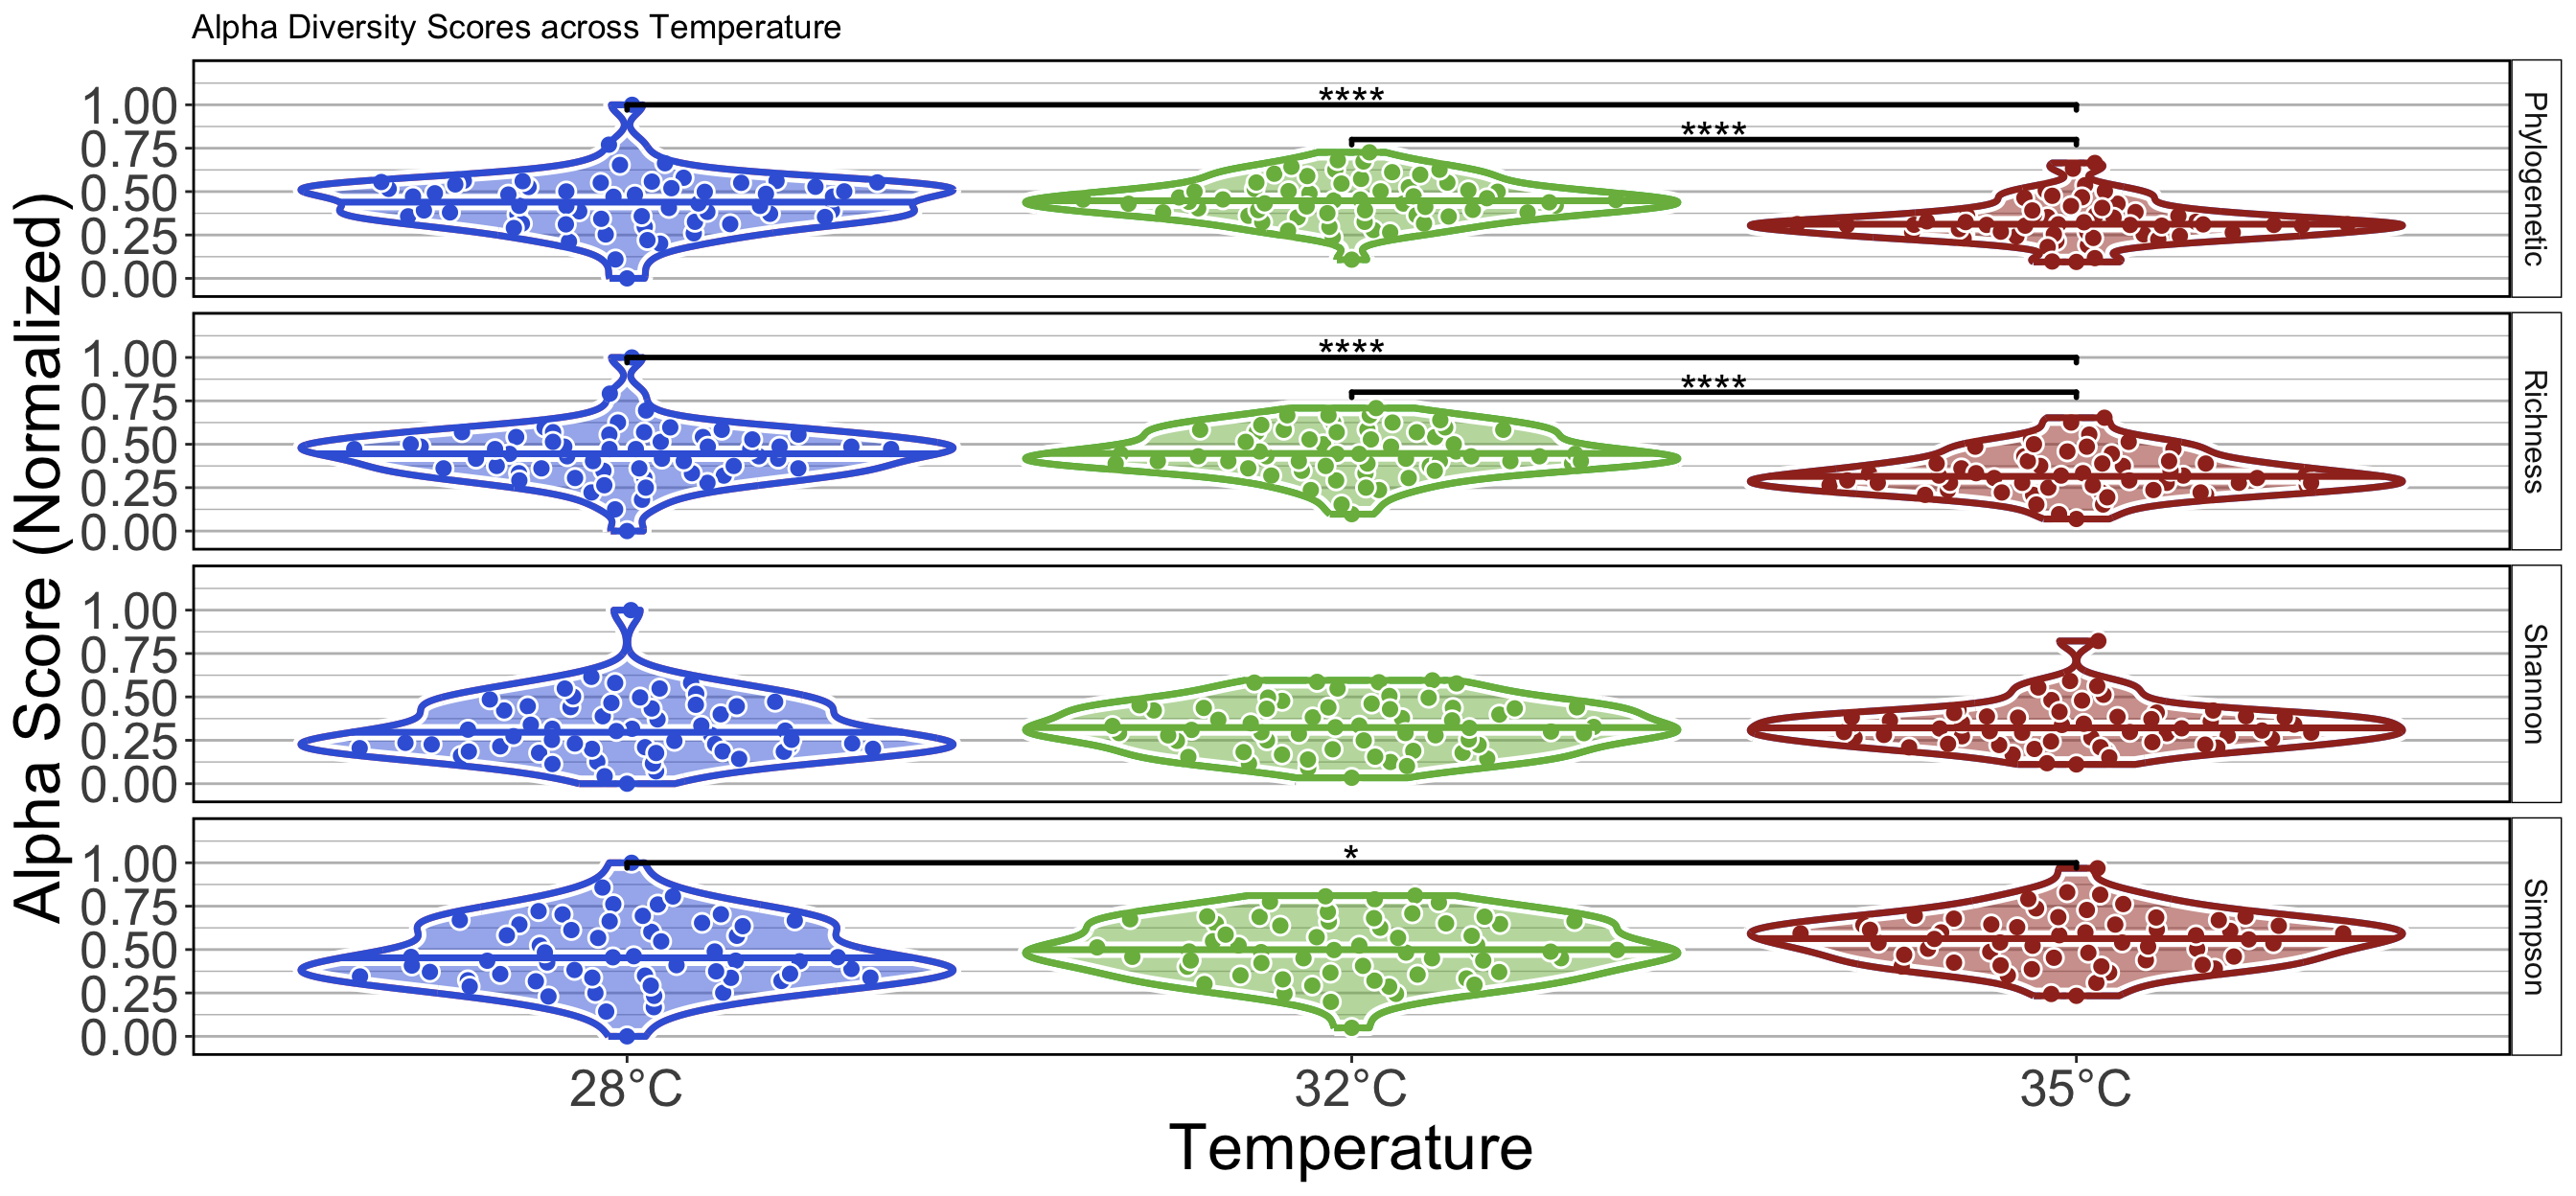
\includegraphics[keepaspectratio]{Results_Overview_files/figure-latex/plots-S2A-1.pdf}}

\paragraph{S2B}\label{s2b}

\pandocbounded{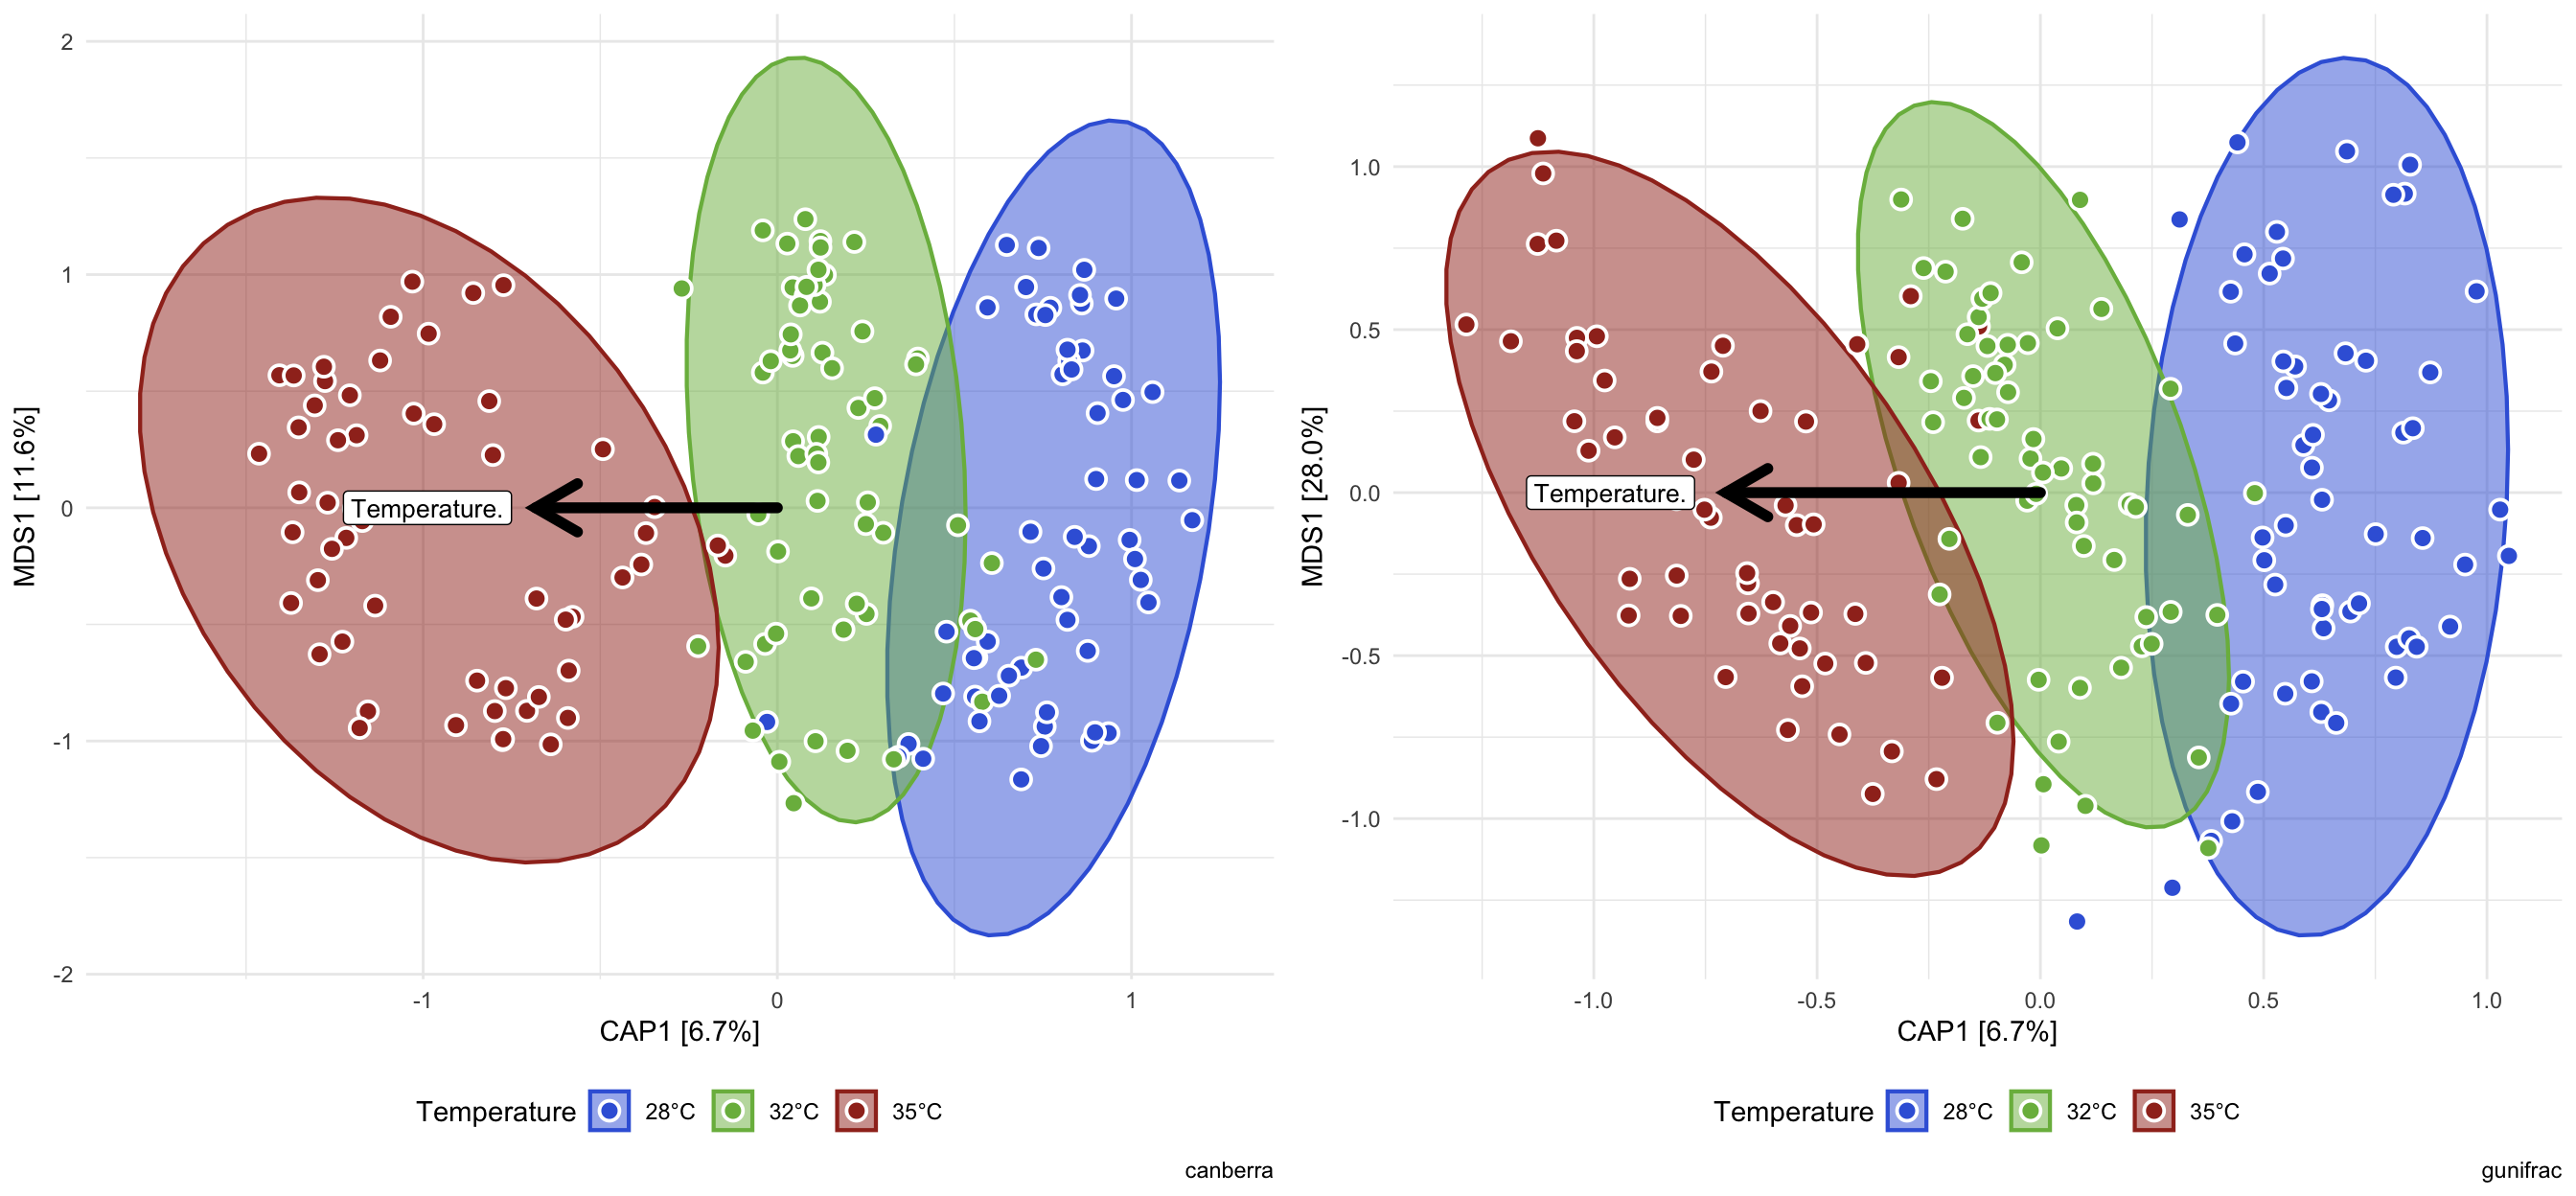
\includegraphics[keepaspectratio]{Results_Overview_files/figure-latex/plots-S2B-1.pdf}}

\paragraph{S2C}\label{s2c}

\pandocbounded{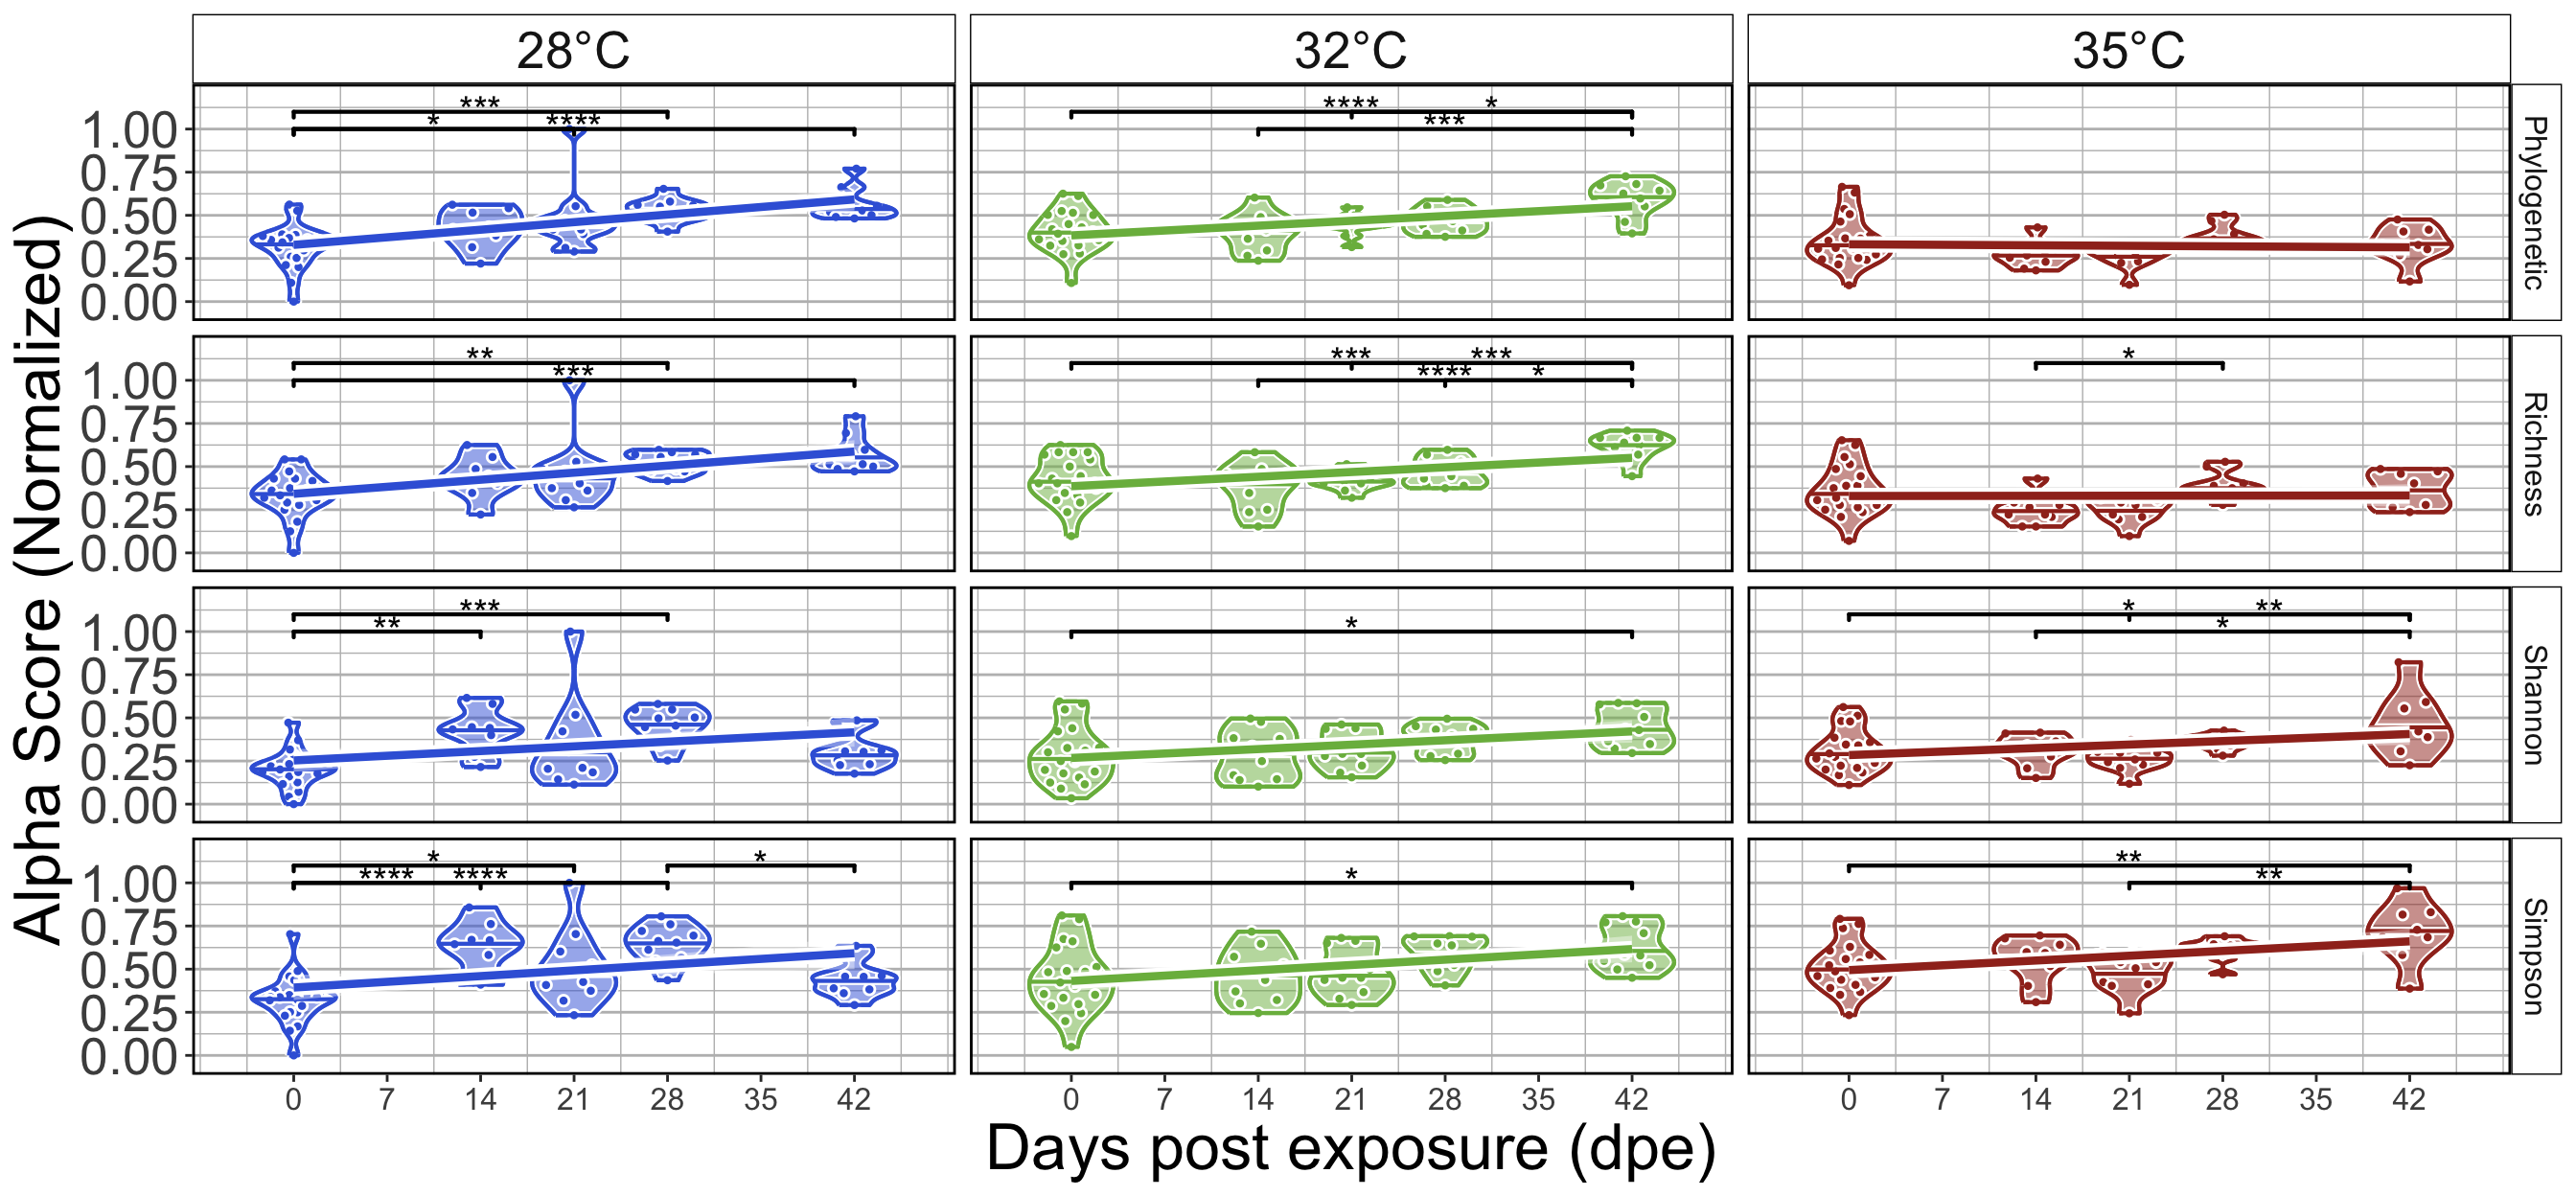
\includegraphics[keepaspectratio]{Results_Overview_files/figure-latex/plots-S2C-1.pdf}}

\paragraph{S2D}\label{s2d}

\pandocbounded{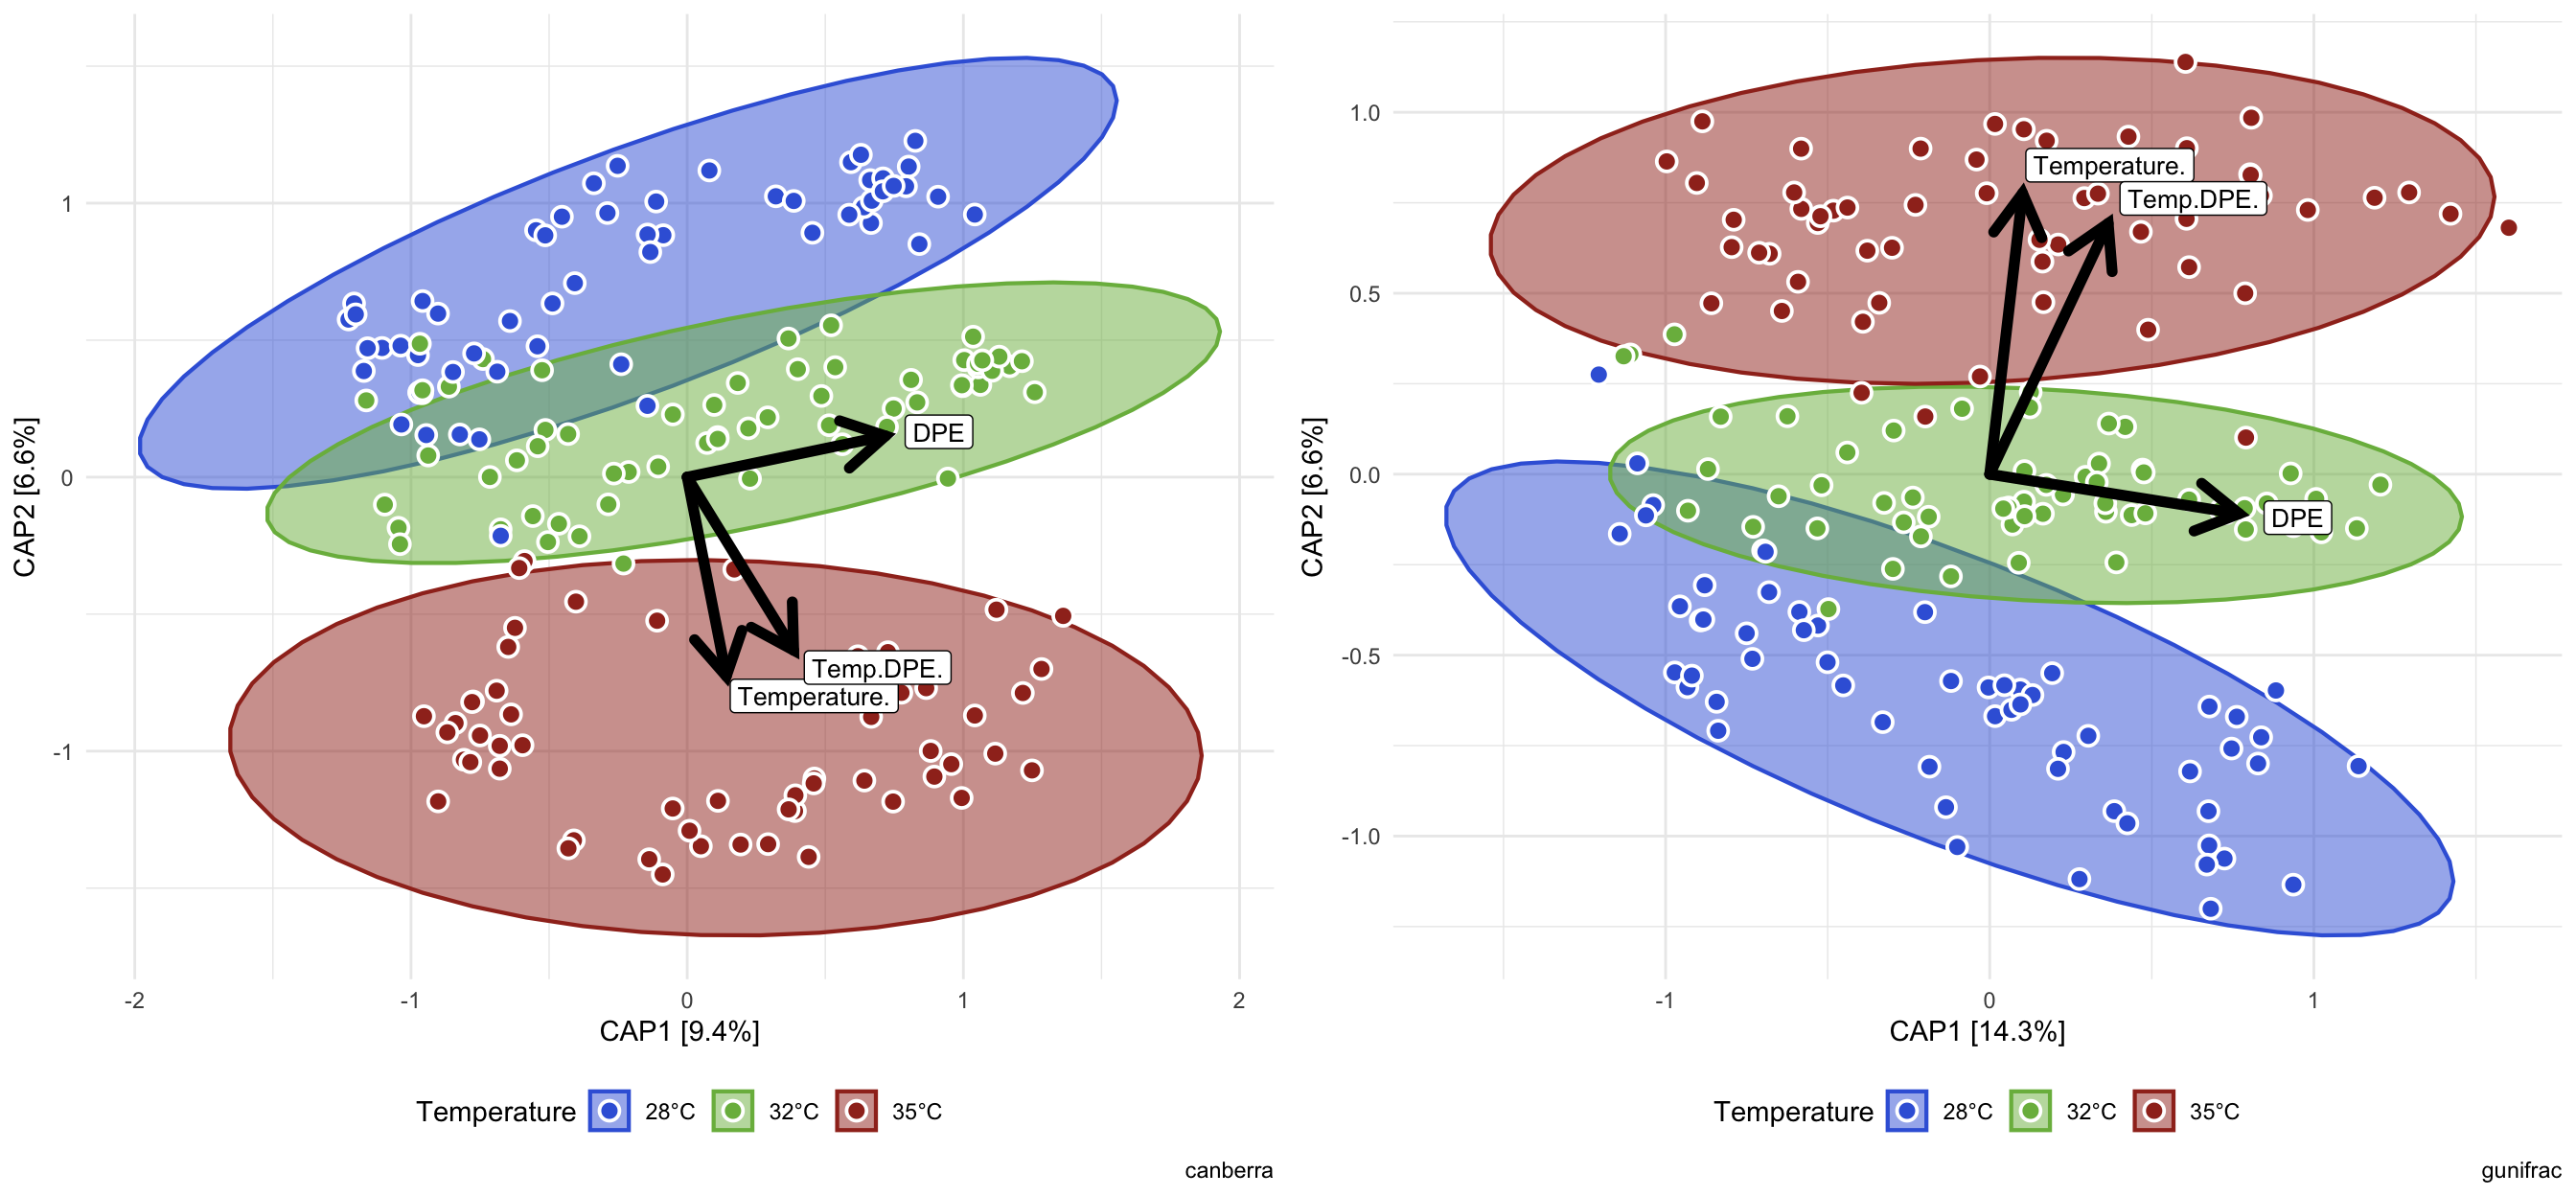
\includegraphics[keepaspectratio]{Results_Overview_files/figure-latex/plots-S2D-1.pdf}}

\subsubsection{Fig. 3) Infection burden is highest in fish reared at
lower water
temperatures}\label{fig.-3-infection-burden-is-highest-in-fish-reared-at-lower-water-temperatures}

\textbf{Fig. 3} Infection outcomes in zebrafish exposed to
Pseudocapillaria tomentosa. (A) Histological sections stained with
\#\#\# stain in zebrafish exposed to P. tomentosa examined at \#\#\#
days post exposure. Nematodes in intestinal lumen. Arrow = \#\#\#. (B)
Infection outcome analysis of fish exposed to P. tomentosa (n = 89) by
temperature. Fish reared at 28°C and 32°C water temperatures had
significantly different infection burden to fish reared at 35°C water
temperature. Only one fish reared at 35°C was identified as being
positively infected by wet mount. Only statistically significant
relationships are shown. A ``*'' indicates statistical significance
below the ``0.05'' level.

\paragraph{3A)}\label{a-1}

\includegraphics[width=3.35in]{Manuscript/Main_Figures/Fig3A}

\paragraph{3B)}\label{b-1}

\pandocbounded{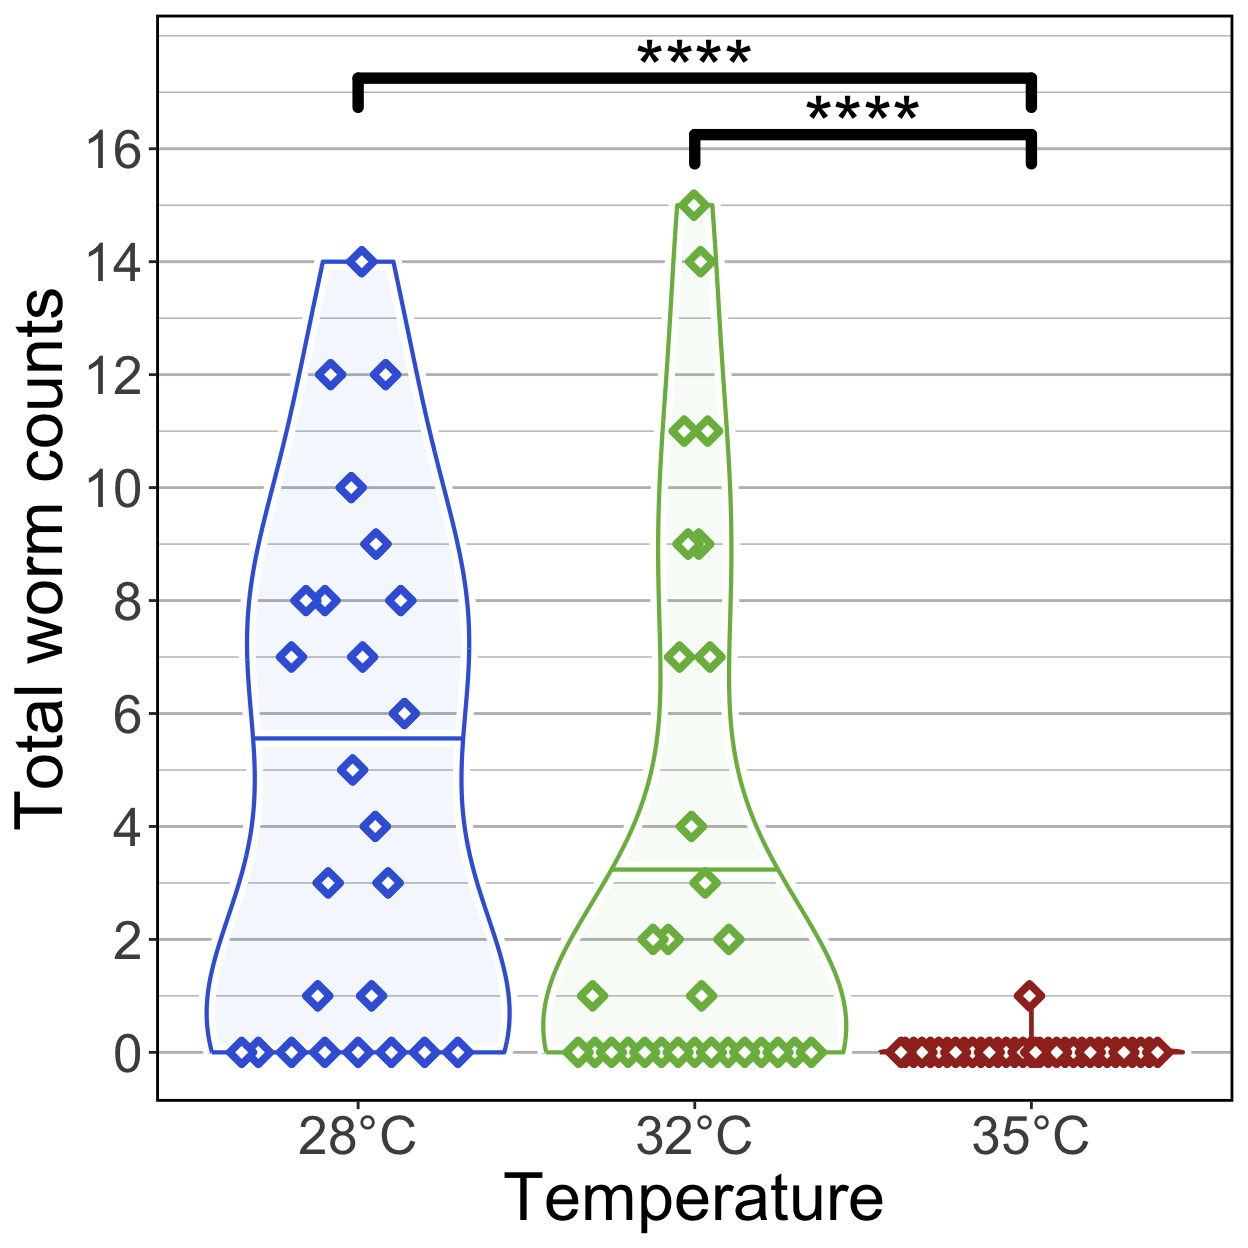
\includegraphics[keepaspectratio]{Results_Overview_files/figure-latex/plots-3B-1.pdf}}

\subparagraph{Tables}\label{tables-4}

(hide)

Click on tabs to display tables. Scroll to see additional rows.

GLM

\begin{longtable}{lrrrrl}
\caption*{
{\large GLM Results} \\ 
{\small glm.nb(Total.Worm.Count \textasciitilde{} Temperature); Exposed fish}
} \\ 
\toprule
term & estimate & std.error & statistic & p.value & p.adj.sig \\ 
\midrule\addlinespace[2.5pt]
(Intercept) & $1.552$ & $0.316$ & $4.914$ & <0.001 & **** \\ 
Temperature32 & $-0.368$ & $0.431$ & $-0.853$ & $\geq$0.25 & ns \\ 
Temperature35 & $-5.078$ & $1.080$ & $-4.701$ & <0.001 & **** \\ 
\bottomrule
\end{longtable}

ANOVA

\begin{longtable}{lrrr}
\caption*{
{\large ANOVA of GLM} \\ 
{\small ANOVA(GLM.NB(Total.Worm.Count \textasciitilde{} Temperature), type = 2); Exposed fish}
} \\ 
\toprule
term & statistic & df & p.value \\ 
\midrule\addlinespace[2.5pt]
Temperature & $55.264$ & $2.000$ & <0.001 \\ 
\bottomrule
\end{longtable}

Tukey

\begin{longtable}{llrrrrrrr}
\caption*{
{\large Pairwise Tukey's HSD, p.adj: Dunnett} \\ 
{\small Tukey(Total.Worm.Count \textasciitilde{} Temperature); Exposed fish}
} \\ 
\toprule
term & .y. & group1 & group2 & estimate & std.error & df & statistic & adj.p.value \\ 
\midrule\addlinespace[2.5pt]
Temperature & Total.Worm.Count & 28 & 32 & $0.368$ & $0.431$ & $ Inf$ & $0.853$ & $\geq$0.25 \\ 
Temperature & Total.Worm.Count & 28 & 35 & $5.078$ & $1.080$ & $ Inf$ & $4.701$ & <0.001 \\ 
Temperature & Total.Worm.Count & 32 & 35 & $4.710$ & $1.074$ & $ Inf$ & $4.386$ & <0.001 \\ 
\bottomrule
\end{longtable}

\paragraph{Suppl.}\label{suppl.}

\subsubsection{}\label{section-1}

\paragraph{(hide)}\label{hide-6}

Click on tabs to reveal supplementary figures and tables.

\paragraph{S3B Counts}\label{s3b-counts}

\subparagraph{Pathology Results}\label{pathology-results}

\begin{longtable}{lr}
\caption*{
{\large Summary of Infection Outcomes} \\ 
{\small (Pathology Results)}
} \\ 
\toprule
Pathology.Results & Count \\ 
\midrule\addlinespace[2.5pt]
\multicolumn{2}{l}{28} \\ 
\midrule\addlinespace[2.5pt]
negative & $8$ \\ 
positive & $17$ \\ 
\midrule\addlinespace[2.5pt]
\multicolumn{2}{l}{32} \\ 
\midrule\addlinespace[2.5pt]
negative & $15$ \\ 
positive & $15$ \\ 
\midrule\addlinespace[2.5pt]
\multicolumn{2}{l}{35} \\ 
\midrule\addlinespace[2.5pt]
negative & $33$ \\ 
positive & $1$ \\ 
\bottomrule
\end{longtable}

\subparagraph{Total Worm Counts}\label{total-worm-counts}

\begin{longtable}{rlrrrrr}
\caption*{
{\large Summary of Infection Outcomes} \\ 
{\small (Total Worm Count)}
} \\ 
\toprule
Group & Variable & Mean & SD & Min & Max & n\_Missing \\ 
\midrule\addlinespace[2.5pt]
28 & Total.Worm.Count & $5$ & $5$ & $0$ & $14$ & $0$ \\ 
32 & Total.Worm.Count & $3$ & $5$ & $0$ & $15$ & $0$ \\ 
35 & Total.Worm.Count & $0$ & $0$ & $0$ & $1$ & $0$ \\ 
\bottomrule
\end{longtable}

\subparagraph{Method}\label{method}

\pandocbounded{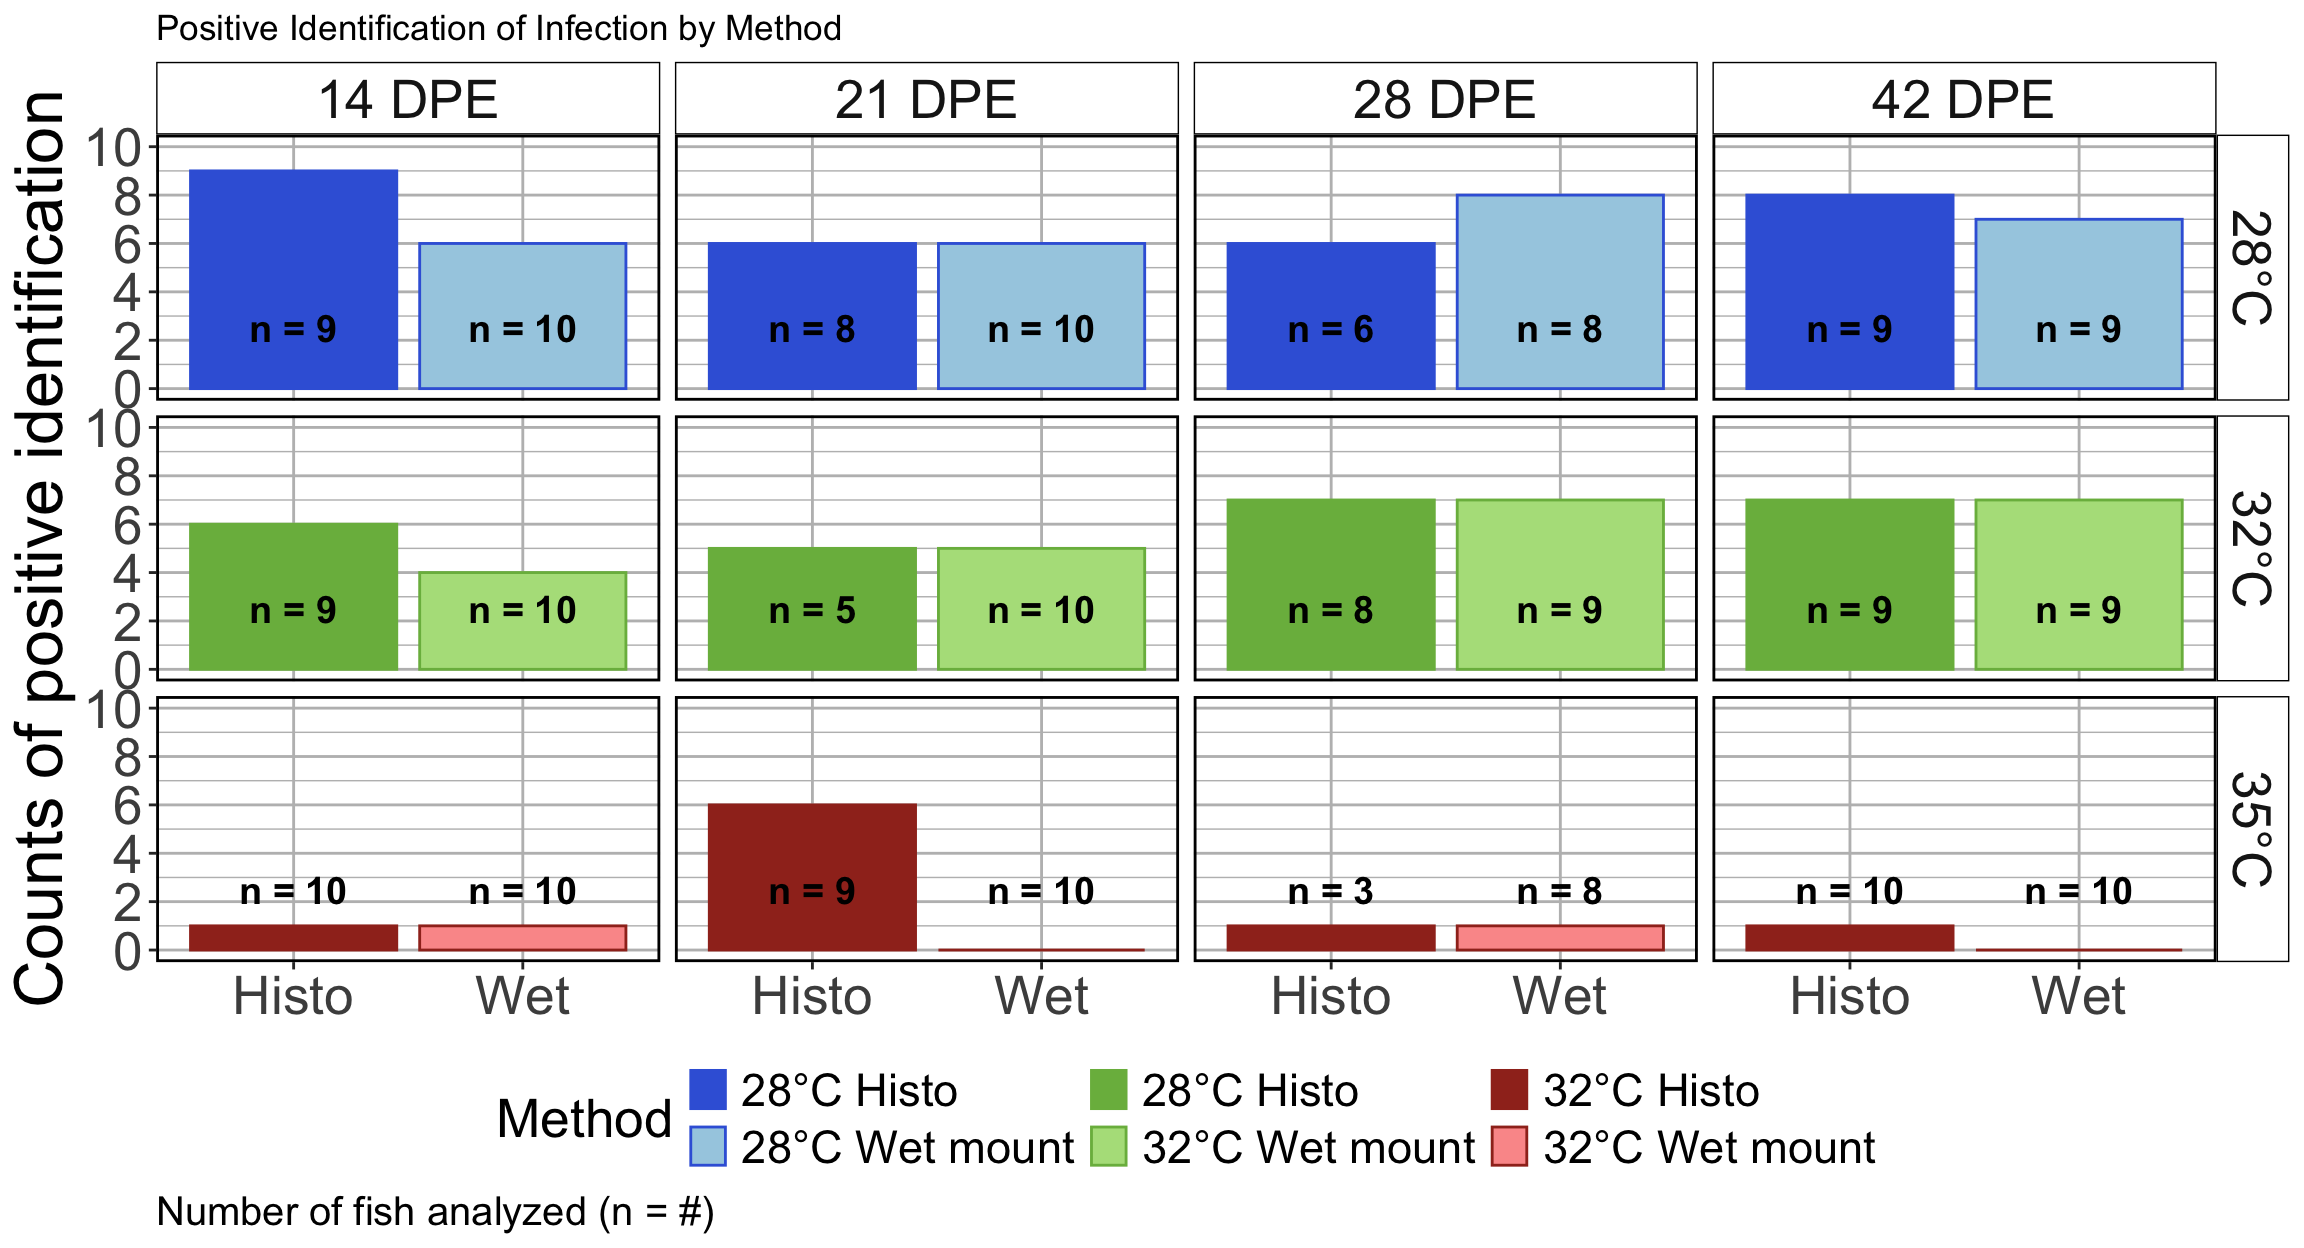
\includegraphics[keepaspectratio]{Results_Overview_files/figure-latex/plots-S3-MethodCount-1-1.pdf}}

\paragraph{S3-X.1}\label{s3-x.1}

\pandocbounded{\includegraphics[keepaspectratio]{Results_Overview_files/figure-latex/plots-S3-X-1-1.pdf}}

\subparagraph{Tables}\label{tables-5}

(hide)

Click on tabs to display tables. Scroll to see additional rows.

GLM

\begin{longtable}{lrrrrl}
\caption*{
{\large GLM Results} \\ 
{\small glm.nb(Total.Worm.Count \textasciitilde{} Temperature*DPE); Exposed fish}
} \\ 
\toprule
term & estimate & std.error & statistic & p.value & p.adj.sig \\ 
\midrule\addlinespace[2.5pt]
(Intercept) & $0.535$ & $0.795$ & $0.673$ & $\geq$0.25 & ns \\ 
Temperature32 & $0.233$ & $1.081$ & $0.216$ & $\geq$0.25 & ns \\ 
Temperature35 & $-4.474$ & $2.964$ & $-1.509$ & $0.131$ & ns \\ 
DPE & $0.035$ & $0.027$ & $1.304$ & $0.192$ & ns \\ 
Temperature32:DPE & $-0.019$ & $0.038$ & $-0.501$ & $\geq$0.25 & ns \\ 
Temperature35:DPE & $-0.020$ & $0.099$ & $-0.200$ & $\geq$0.25 & ns \\ 
\bottomrule
\end{longtable}

ANOVA

\begin{longtable}{lrrr}
\caption*{
{\large ANOVA of GLM} \\ 
{\small ANOVA(GLM.NB(Total.Worm.Count \textasciitilde{} Temperature*DPE), type = 2); Exposed fish}
} \\ 
\toprule
term & statistic & df & p.value \\ 
\midrule\addlinespace[2.5pt]
Temperature & $56.284$ & $2.000$ & <0.001 \\ 
DPE & $1.790$ & $1.000$ & $0.181$ \\ 
Temperature:DPE & $0.265$ & $2.000$ & $\geq$0.25 \\ 
\bottomrule
\end{longtable}

Tukey

\begin{longtable}{cllrrrrrrr}
\caption*{
{\large Pairwise Tukey's HSD, p.adj: Dunnett} \\ 
{\small Tukey(Total.Worm.Count \textasciitilde{} Temperature*DPE); Exposed fish}
} \\ 
\toprule
DPE & .y. & term & group1 & group2 & estimate & std.error & df & statistic & adj.p.value \\ 
\midrule\addlinespace[2.5pt]
14 & Total.Worm.Count & Temperature & 28 & 32 & $-0.229$ & $0.279$ & $ Inf$ & $-0.820$ & $\geq$0.25 \\ 
14 & Total.Worm.Count & Temperature & 28 & 35 & $38.009$ & $22369621.333$ & $ Inf$ & $0.000$ & $\geq$0.25 \\ 
14 & Total.Worm.Count & Temperature & 32 & 35 & $38.238$ & $22369621.333$ & $ Inf$ & $0.000$ & $\geq$0.25 \\ 
21 & Total.Worm.Count & Temperature & 28 & 32 & $0.560$ & $0.392$ & $ Inf$ & $1.427$ & $\geq$0.25 \\ 
21 & Total.Worm.Count & Temperature & 28 & 35 & $38.222$ & $23726566.406$ & $ Inf$ & $0.000$ & $\geq$0.25 \\ 
21 & Total.Worm.Count & Temperature & 32 & 35 & $37.663$ & $23726566.406$ & $ Inf$ & $0.000$ & $\geq$0.25 \\ 
28 & Total.Worm.Count & Temperature & 28 & 32 & $0.605$ & $0.582$ & $ Inf$ & $1.040$ & $\geq$0.25 \\ 
28 & Total.Worm.Count & Temperature & 28 & 35 & $3.837$ & $1.121$ & $ Inf$ & $3.422$ & $0.002$ \\ 
28 & Total.Worm.Count & Temperature & 32 & 35 & $3.232$ & $1.119$ & $ Inf$ & $2.888$ & $0.011$ \\ 
42 & Total.Worm.Count & Temperature & 28 & 32 & $0.377$ & $0.620$ & $ Inf$ & $0.609$ & $\geq$0.25 \\ 
42 & Total.Worm.Count & Temperature & 28 & 35 & $21.230$ & $3142.206$ & $ Inf$ & $0.007$ & $\geq$0.25 \\ 
42 & Total.Worm.Count & Temperature & 32 & 35 & $20.853$ & $3142.206$ & $ Inf$ & $0.007$ & $\geq$0.25 \\ 
\bottomrule
\end{longtable}

\paragraph{S3-X.2}\label{s3-x.2}

\pandocbounded{\includegraphics[keepaspectratio]{Results_Overview_files/figure-latex/plots-S3-X-2-1.pdf}}

\subparagraph{Tables}\label{tables-6}

(hide)

Click on tabs to display tables. Scroll to see additional rows.

GLM

\begin{longtable}{lrrrrl}
\caption*{
{\large GLM Results} \\ 
{\small glm.nb(Total.Worm.Count \textasciitilde{} Temperature*DPE); Exposed fish}
} \\ 
\toprule
term & estimate & std.error & statistic & p.value & p.adj.sig \\ 
\midrule\addlinespace[2.5pt]
(Intercept) & $0.535$ & $0.795$ & $0.673$ & $\geq$0.25 & ns \\ 
Temperature32 & $0.233$ & $1.081$ & $0.216$ & $\geq$0.25 & ns \\ 
Temperature35 & $-4.474$ & $2.964$ & $-1.509$ & $0.131$ & ns \\ 
DPE & $0.035$ & $0.027$ & $1.304$ & $0.192$ & ns \\ 
Temperature32:DPE & $-0.019$ & $0.038$ & $-0.501$ & $\geq$0.25 & ns \\ 
Temperature35:DPE & $-0.020$ & $0.099$ & $-0.200$ & $\geq$0.25 & ns \\ 
\bottomrule
\end{longtable}

ANOVA

\begin{longtable}{lrrr}
\caption*{
{\large ANOVA of GLM} \\ 
{\small ANOVA(GLM.NB(Total.Worm.Count \textasciitilde{} Temperature*DPE), type = 2); Exposed fish}
} \\ 
\toprule
term & statistic & df & p.value \\ 
\midrule\addlinespace[2.5pt]
Temperature & $56.284$ & $2.000$ & <0.001 \\ 
DPE & $1.790$ & $1.000$ & $0.181$ \\ 
Temperature:DPE & $0.265$ & $2.000$ & $\geq$0.25 \\ 
\bottomrule
\end{longtable}

\subsubsection{Fig. 4) Gut microbiome response to parasite exposure
varies across water
temperature}\label{fig.-4-gut-microbiome-response-to-parasite-exposure-varies-across-water-temperature}

\textbf{Fig. 4} Effects of Pseudocapillaria tomentosa exposure on
zebrafish gut microbiomes reared at different water temperatures. (A)
Simpson's Index of diversity shows that gut microbiome diversity
significantly differs between fish reared at 28°C water temperature to
fish reared at 32°C and 35°C water temperatures. (B) Capscale ordination
based on the Bray-Curtis dissimilarity of gut microbiome composition
constrained on the main effect of temperature. The analysis shows that
gut microbiome composition significantly differs between parasite
exposed fish reared at different water temperatures. (C) Simpson's Index
of diversity shows microbial gut diversity decreases with time from 0
days post exposure (dpe) to 42 dpe in parasite exposed fish reared at
28°C water temperature. (D) Capscale ordination of gut microbiome
composition based on the Canberra dissimilarity constrained on the main
effects of water temperature and time (days post exposure, dpe), and
their interaction. The analysis shows that shows that gut microbiome
composition differs between parasite exposed fish across time depending
on water temperature. Ribbons and ellipses indicate 95\% confidence
interval. Only statistically significant relationships are shown. A
``*'' indicates statistical significance below the ``0.05'' level. Black
arrows indicate direction of greatest change in the indicated
covariates.

\paragraph{4A)}\label{a-2}

\pandocbounded{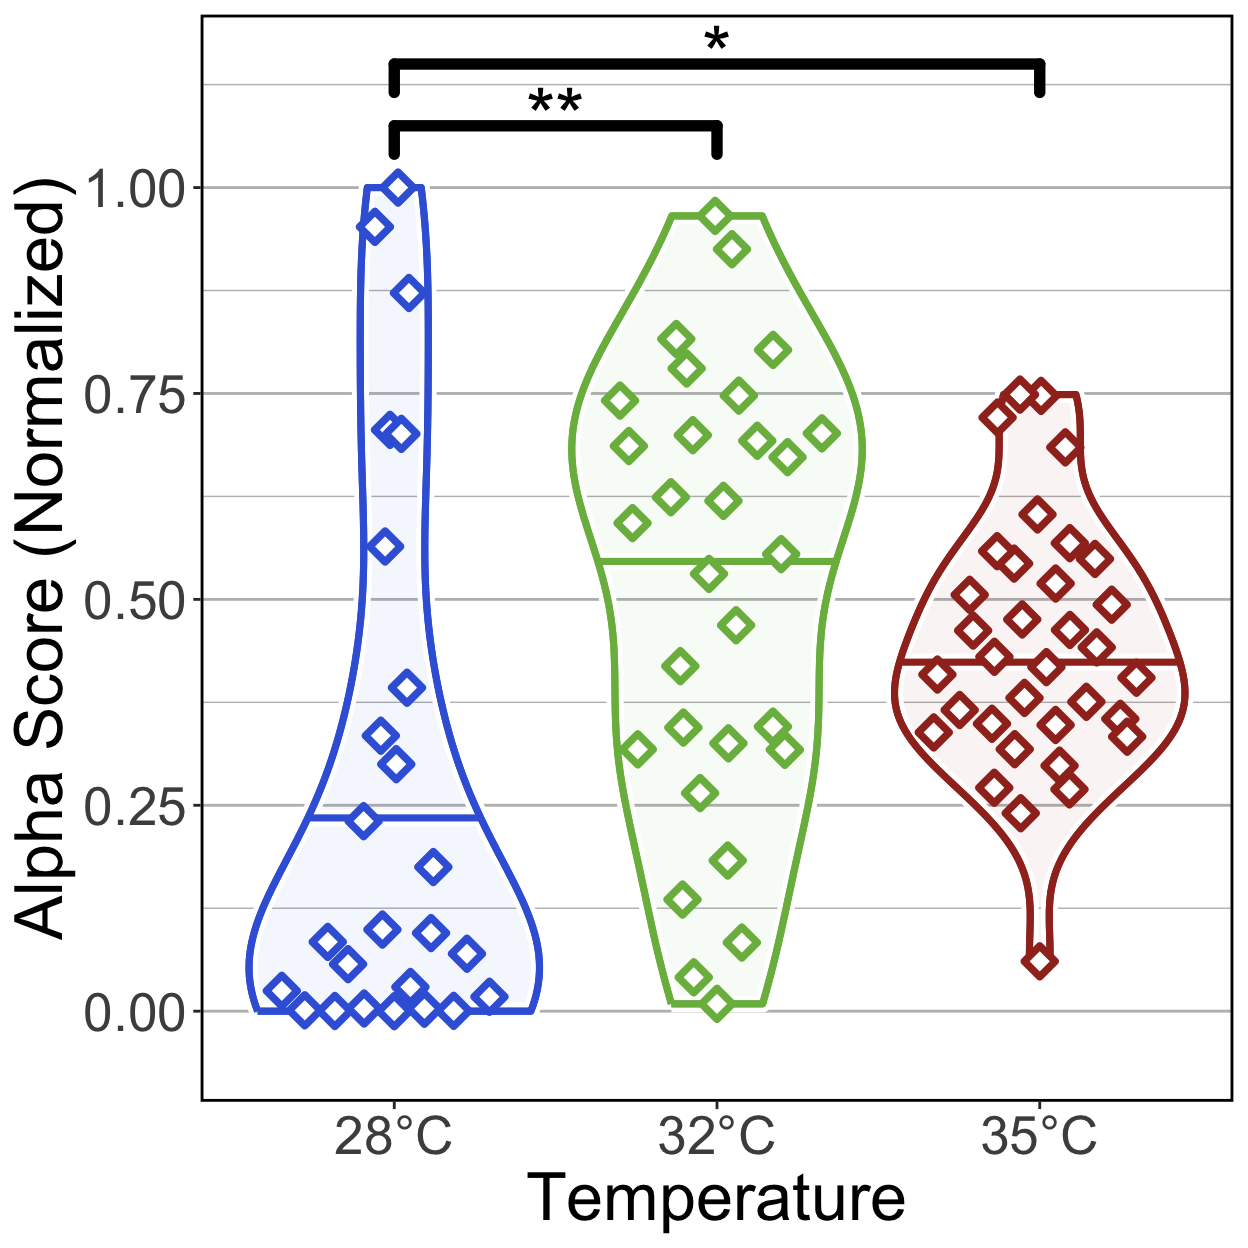
\includegraphics[keepaspectratio]{Results_Overview_files/figure-latex/plots-4A-1.pdf}}

\subparagraph{Tables}\label{tables-7}

(hide)

Click on tabs to display tables. Scroll to see additional rows.

GLM

\begin{longtable}{lrrrrl}
\caption*{
{\large GLM Results} \\ 
{\small glm(Alpha.Score \textasciitilde{} Temperature); Exposed fish}
} \\ 
\toprule
term & estimate & std.error & statistic & p.value & p.adj.sig \\ 
\midrule\addlinespace[2.5pt]
\multicolumn{6}{l}{Shannon} \\ 
\midrule\addlinespace[2.5pt]
(Intercept) & $-0.936$ & $0.233$ & $-4.021$ & <0.001 & *** \\ 
Temperature32 & $0.909$ & $0.301$ & $3.017$ & $0.003$ & ** \\ 
Temperature35 & $0.516$ & $0.296$ & $1.741$ & $0.085$ & ns \\ 
\midrule\addlinespace[2.5pt]
\multicolumn{6}{l}{Simpson} \\ 
\midrule\addlinespace[2.5pt]
(Intercept) & $-1.002$ & $0.243$ & $-4.130$ & <0.001 & **** \\ 
Temperature32 & $1.057$ & $0.312$ & $3.384$ & $0.001$ & ** \\ 
Temperature35 & $0.772$ & $0.306$ & $2.525$ & $0.013$ & * \\ 
\midrule\addlinespace[2.5pt]
\multicolumn{6}{l}{Richness} \\ 
\midrule\addlinespace[2.5pt]
(Intercept) & $-0.681$ & $0.190$ & $-3.583$ & <0.001 & *** \\ 
Temperature32 & $0.703$ & $0.251$ & $2.800$ & $0.006$ & ** \\ 
Temperature35 & $0.242$ & $0.247$ & $0.978$ & $\geq$0.25 & ns \\ 
\midrule\addlinespace[2.5pt]
\multicolumn{6}{l}{Phylogenetic} \\ 
\midrule\addlinespace[2.5pt]
(Intercept) & $-0.681$ & $0.180$ & $-3.789$ & <0.001 & *** \\ 
Temperature32 & $0.648$ & $0.237$ & $2.730$ & $0.008$ & ** \\ 
Temperature35 & $0.161$ & $0.235$ & $0.688$ & $\geq$0.25 & ns \\ 
\bottomrule
\end{longtable}

ANOVA

\begin{longtable}{lrrrr}
\caption*{
{\large ANOVA of GLM} \\ 
{\small ANOVA(GLM(Alpha.Score \textasciitilde{} Temperature), type = 2); Exposed fish}
} \\ 
\toprule
term & statistic & df & p.value & sig \\ 
\midrule\addlinespace[2.5pt]
\multicolumn{5}{l}{Shannon} \\ 
\midrule\addlinespace[2.5pt]
Temperature & $9.440$ & $2.000$ & $0.009$ & ** \\ 
\midrule\addlinespace[2.5pt]
\multicolumn{5}{l}{Simpson} \\ 
\midrule\addlinespace[2.5pt]
Temperature & $12.497$ & $2.000$ & $0.002$ & ** \\ 
\midrule\addlinespace[2.5pt]
\multicolumn{5}{l}{Richness} \\ 
\midrule\addlinespace[2.5pt]
Temperature & $8.575$ & $2.000$ & $0.014$ & * \\ 
\midrule\addlinespace[2.5pt]
\multicolumn{5}{l}{Phylogenetic} \\ 
\midrule\addlinespace[2.5pt]
Temperature & $8.706$ & $2.000$ & $0.013$ & * \\ 
\bottomrule
\end{longtable}

Tukey

\begin{longtable}{llrrrrrrl}
\caption*{
{\large Pairwise Tukey's HSD, p.adj: Dunnett} \\ 
{\small Tukey(Alpha.Score \textasciitilde{} Temperature); Exposed fish}
} \\ 
\toprule
term & .y. & group1 & group2 & estimate & std.error & statistic & adj.p.value & Variable \\ 
\midrule\addlinespace[2.5pt]
\multicolumn{9}{l}{Shannon} \\ 
\midrule\addlinespace[2.5pt]
Temperature & Alpha.Score & 32 & 28 & $0.909$ & $0.301$ & $3.017$ & $0.007$ & Temperature \\ 
Temperature & Alpha.Score & 35 & 28 & $0.516$ & $0.296$ & $1.741$ & $0.190$ & Temperature \\ 
Temperature & Alpha.Score & 35 & 32 & $-0.393$ & $0.265$ & $-1.482$ & $\geq$0.25 & Temperature \\ 
\midrule\addlinespace[2.5pt]
\multicolumn{9}{l}{Simpson} \\ 
\midrule\addlinespace[2.5pt]
Temperature & Alpha.Score & 32 & 28 & $1.057$ & $0.312$ & $3.384$ & $0.002$ & Temperature \\ 
Temperature & Alpha.Score & 35 & 28 & $0.772$ & $0.306$ & $2.525$ & $0.031$ & Temperature \\ 
Temperature & Alpha.Score & 35 & 32 & $-0.285$ & $0.270$ & $-1.054$ & $\geq$0.25 & Temperature \\ 
\midrule\addlinespace[2.5pt]
\multicolumn{9}{l}{Richness} \\ 
\midrule\addlinespace[2.5pt]
Temperature & Alpha.Score & 32 & 28 & $0.703$ & $0.251$ & $2.800$ & $0.014$ & Temperature \\ 
Temperature & Alpha.Score & 35 & 28 & $0.242$ & $0.247$ & $0.978$ & $\geq$0.25 & Temperature \\ 
Temperature & Alpha.Score & 35 & 32 & $-0.461$ & $0.228$ & $-2.028$ & $0.105$ & Temperature \\ 
\midrule\addlinespace[2.5pt]
\multicolumn{9}{l}{Phylogenetic} \\ 
\midrule\addlinespace[2.5pt]
Temperature & Alpha.Score & 32 & 28 & $0.648$ & $0.237$ & $2.730$ & $0.017$ & Temperature \\ 
Temperature & Alpha.Score & 35 & 28 & $0.161$ & $0.235$ & $0.688$ & $\geq$0.25 & Temperature \\ 
Temperature & Alpha.Score & 35 & 32 & $-0.487$ & $0.216$ & $-2.251$ & $0.063$ & Temperature \\ 
\bottomrule
\end{longtable}

\subparagraph{Addl. Metrics}\label{addl.-metrics-4}

\paragraph{4B)}\label{b-2}

\pandocbounded{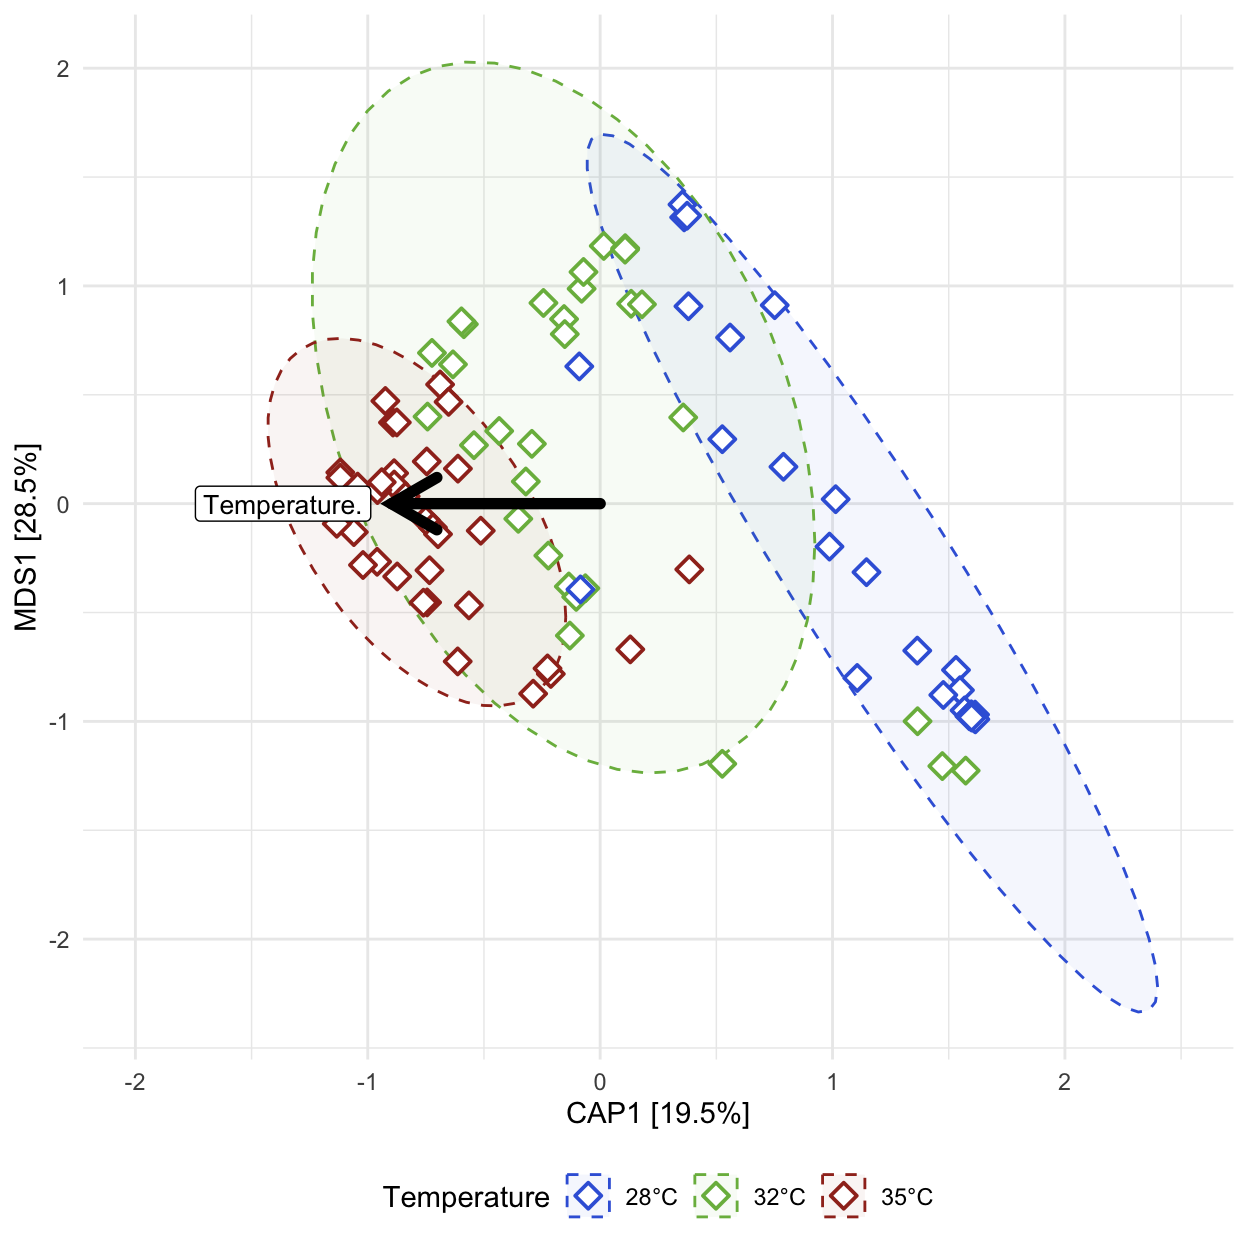
\includegraphics[keepaspectratio]{Results_Overview_files/figure-latex/plots-4B-1.pdf}}

\subparagraph{Tables}\label{tables-8}

(hide)

Click on tabs to display tables. Scroll to see additional rows.

ADONIS2

\begin{longtable}{lrrrrrr}
\caption*{
{\large ADONIS2} \\ 
{\small adonis2(Beta Distance \textasciitilde{} Temperature); Exposed fish}
} \\ 
\toprule
term & df & SumOfSqs & R2 & statistic & p.value & sig \\ 
\midrule\addlinespace[2.5pt]
\multicolumn{7}{l}{bray} \\ 
\midrule\addlinespace[2.5pt]
Temperature & $2.000$ & $5.218$ & $0.251$ & $14.447$ & $0.001$ & *** \\ 
Residual & $86.000$ & $15.530$ & $0.749$ & NA & NA & NA \\ 
Total & $88.000$ & $20.748$ & $1.000$ & NA & NA & NA \\ 
\midrule\addlinespace[2.5pt]
\multicolumn{7}{l}{canberra} \\ 
\midrule\addlinespace[2.5pt]
Temperature & $2.000$ & $3.573$ & $0.117$ & $5.701$ & $0.001$ & *** \\ 
Residual & $86.000$ & $26.947$ & $0.883$ & NA & NA & NA \\ 
Total & $88.000$ & $30.520$ & $1.000$ & NA & NA & NA \\ 
\midrule\addlinespace[2.5pt]
\multicolumn{7}{l}{gunifrac} \\ 
\midrule\addlinespace[2.5pt]
Temperature & $2.000$ & $3.363$ & $0.212$ & $11.590$ & $0.001$ & *** \\ 
Residual & $86.000$ & $12.478$ & $0.788$ & NA & NA & NA \\ 
Total & $88.000$ & $15.841$ & $1.000$ & NA & NA & NA \\ 
\bottomrule
\end{longtable}

Dispersion (ANOVA)

\begin{longtable}{lrrrrrr}
\caption*{
{\large ANOVA: Homogeneity of Dispersion} \\ 
{\small ANOVA(Beta Disperson \textasciitilde{} Temperature); Exposed fish}
} \\ 
\toprule
term & df & sumsq & meansq & statistic & p.value & sig \\ 
\midrule\addlinespace[2.5pt]
\multicolumn{7}{l}{bray} \\ 
\midrule\addlinespace[2.5pt]
Temperature & $2.000$ & $0.364$ & $0.182$ & $8.708$ & <0.001 & *** \\ 
Residual & $86.000$ & $1.796$ & $0.021$ & NA & NA & NA \\ 
\midrule\addlinespace[2.5pt]
\multicolumn{7}{l}{canberra} \\ 
\midrule\addlinespace[2.5pt]
Temperature & $2.000$ & $0.314$ & $0.157$ & $17.419$ & <0.001 & **** \\ 
Residual & $86.000$ & $0.774$ & $0.009$ & NA & NA & NA \\ 
\midrule\addlinespace[2.5pt]
\multicolumn{7}{l}{gunifrac} \\ 
\midrule\addlinespace[2.5pt]
Temperature & $2.000$ & $0.310$ & $0.155$ & $13.567$ & <0.001 & **** \\ 
Residual & $86.000$ & $0.983$ & $0.011$ & NA & NA & NA \\ 
\bottomrule
\end{longtable}

Dispersion (Tukey)

\begin{longtable}{llrrrrrrl}
\caption*{
{\large Tukey: Homogeneity of Dispersion} \\ 
{\small Tukey(Beta Disperson \textasciitilde{} Temperature); Exposed fish}
} \\ 
\toprule
.y. & term & group1 & group2 & estimate & conf.low & conf.high & adj.p.value & sig \\ 
\midrule\addlinespace[2.5pt]
\multicolumn{9}{l}{bray} \\ 
\midrule\addlinespace[2.5pt]
Distance & Temperature & 32 & 28 & $-0.043$ & $-0.136$ & $0.051$ & $\geq$0.25 & ns \\ 
Distance & Temperature & 35 & 28 & $-0.150$ & $-0.241$ & $-0.059$ & <0.001 & *** \\ 
Distance & Temperature & 35 & 32 & $-0.108$ & $-0.194$ & $-0.021$ & $0.011$ & * \\ 
\midrule\addlinespace[2.5pt]
\multicolumn{9}{l}{canberra} \\ 
\midrule\addlinespace[2.5pt]
Distance & Temperature & 32 & 28 & $-0.110$ & $-0.171$ & $-0.049$ & <0.001 & *** \\ 
Distance & Temperature & 35 & 28 & $-0.144$ & $-0.204$ & $-0.085$ & <0.001 & **** \\ 
Distance & Temperature & 35 & 32 & $-0.034$ & $-0.091$ & $0.022$ & $\geq$0.25 & ns \\ 
\midrule\addlinespace[2.5pt]
\multicolumn{9}{l}{gunifrac} \\ 
\midrule\addlinespace[2.5pt]
Distance & Temperature & 32 & 28 & $-0.056$ & $-0.125$ & $0.013$ & $0.133$ & ns \\ 
Distance & Temperature & 35 & 28 & $-0.143$ & $-0.211$ & $-0.076$ & <0.001 & **** \\ 
Distance & Temperature & 35 & 32 & $-0.087$ & $-0.151$ & $-0.023$ & $0.005$ & ** \\ 
\bottomrule
\end{longtable}

\subparagraph{Addl. Metrics}\label{addl.-metrics-5}

\paragraph{4C)}\label{c-1}

\pandocbounded{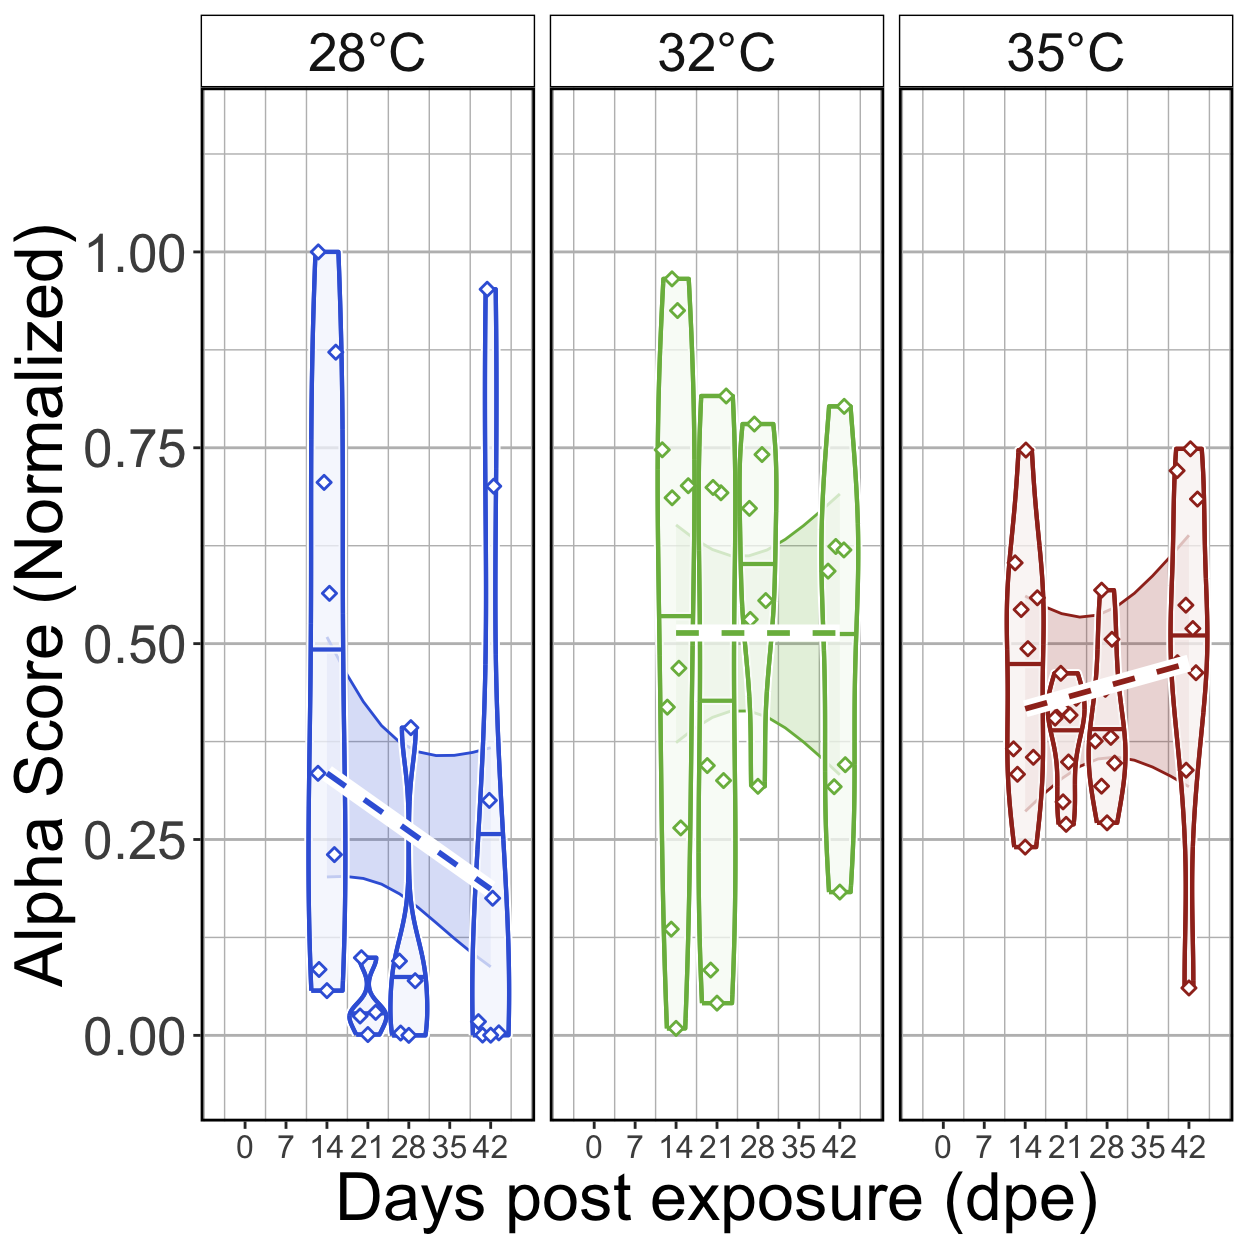
\includegraphics[keepaspectratio]{Results_Overview_files/figure-latex/plots-4C-1.pdf}}

\subparagraph{Tables}\label{tables-9}

(hide)

Click on tabs to display tables. Scroll to see additional rows.

GLM

\begin{longtable}{lrrrrl}
\caption*{
{\large GLM Results} \\ 
{\small glm(Alpha.Score \textasciitilde{} Temperature*DPE); Exposed fish}
} \\ 
\toprule
term & estimate & std.error & statistic & p.value & p.adj.sig \\ 
\midrule\addlinespace[2.5pt]
\multicolumn{6}{l}{Shannon} \\ 
\midrule\addlinespace[2.5pt]
(Intercept) & $-0.134$ & $0.594$ & $-0.226$ & $\geq$0.25 & ns \\ 
Temperature32 & $0.228$ & $0.774$ & $0.295$ & $\geq$0.25 & ns \\ 
Temperature35 & $-0.428$ & $0.777$ & $-0.551$ & $\geq$0.25 & ns \\ 
DPE & $-0.031$ & $0.022$ & $-1.425$ & $0.158$ & ns \\ 
Temperature32:DPE & $0.026$ & $0.028$ & $0.917$ & $\geq$0.25 & ns \\ 
Temperature35:DPE & $0.036$ & $0.028$ & $1.300$ & $0.197$ & ns \\ 
\midrule\addlinespace[2.5pt]
\multicolumn{6}{l}{Simpson} \\ 
\midrule\addlinespace[2.5pt]
(Intercept) & $-0.282$ & $0.617$ & $-0.456$ & $\geq$0.25 & ns \\ 
Temperature32 & $0.336$ & $0.801$ & $0.420$ & $\geq$0.25 & ns \\ 
Temperature35 & $-0.172$ & $0.799$ & $-0.215$ & $\geq$0.25 & ns \\ 
DPE & $-0.028$ & $0.022$ & $-1.234$ & $0.221$ & ns \\ 
Temperature32:DPE & $0.028$ & $0.029$ & $0.946$ & $\geq$0.25 & ns \\ 
Temperature35:DPE & $0.036$ & $0.029$ & $1.261$ & $0.211$ & ns \\ 
\midrule\addlinespace[2.5pt]
\multicolumn{6}{l}{Richness} \\ 
\midrule\addlinespace[2.5pt]
(Intercept) & $0.316$ & $0.480$ & $0.657$ & $\geq$0.25 & ns \\ 
Temperature32 & $-0.034$ & $0.636$ & $-0.054$ & $\geq$0.25 & ns \\ 
Temperature35 & $-0.596$ & $0.638$ & $-0.934$ & $\geq$0.25 & ns \\ 
DPE & $-0.038$ & $0.017$ & $-2.191$ & $0.031$ & * \\ 
Temperature32:DPE & $0.028$ & $0.023$ & $1.199$ & $0.234$ & ns \\ 
Temperature35:DPE & $0.032$ & $0.023$ & $1.405$ & $0.164$ & ns \\ 
\midrule\addlinespace[2.5pt]
\multicolumn{6}{l}{Phylogenetic} \\ 
\midrule\addlinespace[2.5pt]
(Intercept) & $0.305$ & $0.451$ & $0.676$ & $\geq$0.25 & ns \\ 
Temperature32 & $-0.101$ & $0.597$ & $-0.169$ & $\geq$0.25 & ns \\ 
Temperature35 & $-0.766$ & $0.601$ & $-1.274$ & $0.206$ & ns \\ 
DPE & $-0.038$ & $0.016$ & $-2.310$ & $0.023$ & * \\ 
Temperature32:DPE & $0.028$ & $0.022$ & $1.298$ & $0.198$ & ns \\ 
Temperature35:DPE & $0.036$ & $0.022$ & $1.651$ & $0.103$ & ns \\ 
\bottomrule
\end{longtable}

ANOVA

\begin{longtable}{lrrrl}
\caption*{
{\large ANOVA of GLM} \\ 
{\small ANOVA(GLM(Alpha.Score \textasciitilde{} Temperature*Time), type = 2); Exposed fish}
} \\ 
\toprule
term & statistic & df & p.value & sig \\ 
\midrule\addlinespace[2.5pt]
\multicolumn{5}{l}{Shannon} \\ 
\midrule\addlinespace[2.5pt]
Temperature & $8.789$ & $2.000$ & $0.012$ & * \\ 
DPE & $0.523$ & $1.000$ & $\geq$0.25 & ns \\ 
Temperature:DPE & $1.759$ & $2.000$ & $\geq$0.25 & ns \\ 
\midrule\addlinespace[2.5pt]
\multicolumn{5}{l}{Simpson} \\ 
\midrule\addlinespace[2.5pt]
Temperature & $11.871$ & $2.000$ & $0.003$ & ** \\ 
DPE & $0.120$ & $1.000$ & $\geq$0.25 & ns \\ 
Temperature:DPE & $1.684$ & $2.000$ & $\geq$0.25 & ns \\ 
\midrule\addlinespace[2.5pt]
\multicolumn{5}{l}{Richness} \\ 
\midrule\addlinespace[2.5pt]
Temperature & $7.911$ & $2.000$ & $0.019$ & * \\ 
DPE & $3.435$ & $1.000$ & $0.064$ & ns \\ 
Temperature:DPE & $2.255$ & $2.000$ & $\geq$0.25 & ns \\ 
\midrule\addlinespace[2.5pt]
\multicolumn{5}{l}{Phylogenetic} \\ 
\midrule\addlinespace[2.5pt]
Temperature & $8.173$ & $2.000$ & $0.017$ & * \\ 
DPE & $3.103$ & $1.000$ & $0.078$ & ns \\ 
Temperature:DPE & $2.980$ & $2.000$ & $0.225$ & ns \\ 
\bottomrule
\end{longtable}

Tukey

\begin{longtable}{cllrrrrrrlc}
\caption*{
{\large Pairwise Tukey's HSD, p.adj: Dunnett} \\ 
{\small Tukey(Alpha.Score \textasciitilde{} Temperature*Time); Exposed fish}
} \\ 
\toprule
Temperature & .y. & term & group1 & group2 & estimate & std.error & statistic & adj.p.value & Variable & Group \\ 
\midrule\addlinespace[2.5pt]
\multicolumn{11}{l}{Shannon} \\ 
\midrule\addlinespace[2.5pt]
28 & Alpha.Score & DPE & 21 & 14 & $-3.311$ & $1.822$ & $-1.817$ & $0.246$ & DPE & 28 \\ 
28 & Alpha.Score & DPE & 28 & 14 & $-2.027$ & $1.023$ & $-1.982$ & $0.178$ & DPE & 28 \\ 
28 & Alpha.Score & DPE & 42 & 14 & $-1.024$ & $0.705$ & $-1.452$ & $\geq$0.25 & DPE & 28 \\ 
28 & Alpha.Score & DPE & 28 & 21 & $1.284$ & $1.982$ & $0.648$ & $\geq$0.25 & DPE & 28 \\ 
28 & Alpha.Score & DPE & 42 & 21 & $2.287$ & $1.838$ & $1.245$ & $\geq$0.25 & DPE & 28 \\ 
28 & Alpha.Score & DPE & 42 & 28 & $1.004$ & $1.050$ & $0.956$ & $\geq$0.25 & DPE & 28 \\ 
32 & Alpha.Score & DPE & 21 & 14 & $-0.536$ & $0.537$ & $-0.999$ & $\geq$0.25 & DPE & 32 \\ 
32 & Alpha.Score & DPE & 28 & 14 & $0.056$ & $0.558$ & $0.099$ & $\geq$0.25 & DPE & 32 \\ 
32 & Alpha.Score & DPE & 42 & 14 & $-0.271$ & $0.532$ & $-0.509$ & $\geq$0.25 & DPE & 32 \\ 
32 & Alpha.Score & DPE & 28 & 21 & $0.592$ & $0.606$ & $0.977$ & $\geq$0.25 & DPE & 32 \\ 
32 & Alpha.Score & DPE & 42 & 21 & $0.266$ & $0.581$ & $0.457$ & $\geq$0.25 & DPE & 32 \\ 
32 & Alpha.Score & DPE & 42 & 28 & $-0.326$ & $0.601$ & $-0.543$ & $\geq$0.25 & DPE & 32 \\ 
35 & Alpha.Score & DPE & 21 & 14 & $-0.246$ & $0.270$ & $-0.909$ & $\geq$0.25 & DPE & 35 \\ 
35 & Alpha.Score & DPE & 28 & 14 & $-0.292$ & $0.271$ & $-1.075$ & $\geq$0.25 & DPE & 35 \\ 
35 & Alpha.Score & DPE & 42 & 14 & $0.097$ & $0.258$ & $0.377$ & $\geq$0.25 & DPE & 35 \\ 
35 & Alpha.Score & DPE & 28 & 21 & $-0.046$ & $0.283$ & $-0.162$ & $\geq$0.25 & DPE & 35 \\ 
35 & Alpha.Score & DPE & 42 & 21 & $0.343$ & $0.270$ & $1.273$ & $\geq$0.25 & DPE & 35 \\ 
35 & Alpha.Score & DPE & 42 & 28 & $0.389$ & $0.271$ & $1.438$ & $\geq$0.25 & DPE & 35 \\ 
\midrule\addlinespace[2.5pt]
\multicolumn{11}{l}{Simpson} \\ 
\midrule\addlinespace[2.5pt]
28 & Alpha.Score & DPE & 21 & 14 & $-3.141$ & $1.820$ & $-1.725$ & $\geq$0.25 & DPE & 28 \\ 
28 & Alpha.Score & DPE & 28 & 14 & $-1.994$ & $1.072$ & $-1.861$ & $0.227$ & DPE & 28 \\ 
28 & Alpha.Score & DPE & 42 & 14 & $-0.925$ & $0.721$ & $-1.283$ & $\geq$0.25 & DPE & 28 \\ 
28 & Alpha.Score & DPE & 28 & 21 & $1.147$ & $2.001$ & $0.573$ & $\geq$0.25 & DPE & 28 \\ 
28 & Alpha.Score & DPE & 42 & 21 & $2.215$ & $1.837$ & $1.206$ & $\geq$0.25 & DPE & 28 \\ 
28 & Alpha.Score & DPE & 42 & 28 & $1.069$ & $1.100$ & $0.971$ & $\geq$0.25 & DPE & 28 \\ 
32 & Alpha.Score & DPE & 21 & 14 & $-0.416$ & $0.550$ & $-0.756$ & $\geq$0.25 & DPE & 32 \\ 
32 & Alpha.Score & DPE & 28 & 14 & $0.275$ & $0.580$ & $0.474$ & $\geq$0.25 & DPE & 32 \\ 
32 & Alpha.Score & DPE & 42 & 14 & $-0.138$ & $0.546$ & $-0.252$ & $\geq$0.25 & DPE & 32 \\ 
32 & Alpha.Score & DPE & 28 & 21 & $0.691$ & $0.626$ & $1.103$ & $\geq$0.25 & DPE & 32 \\ 
32 & Alpha.Score & DPE & 42 & 21 & $0.278$ & $0.595$ & $0.467$ & $\geq$0.25 & DPE & 32 \\ 
32 & Alpha.Score & DPE & 42 & 28 & $-0.413$ & $0.623$ & $-0.662$ & $\geq$0.25 & DPE & 32 \\ 
35 & Alpha.Score & DPE & 21 & 14 & $-0.374$ & $0.297$ & $-1.258$ & $\geq$0.25 & DPE & 35 \\ 
35 & Alpha.Score & DPE & 28 & 14 & $-0.285$ & $0.296$ & $-0.966$ & $\geq$0.25 & DPE & 35 \\ 
35 & Alpha.Score & DPE & 42 & 14 & $0.142$ & $0.284$ & $0.502$ & $\geq$0.25 & DPE & 35 \\ 
35 & Alpha.Score & DPE & 28 & 21 & $0.088$ & $0.308$ & $0.287$ & $\geq$0.25 & DPE & 35 \\ 
35 & Alpha.Score & DPE & 42 & 21 & $0.516$ & $0.297$ & $1.738$ & $\geq$0.25 & DPE & 35 \\ 
35 & Alpha.Score & DPE & 42 & 28 & $0.428$ & $0.295$ & $1.448$ & $\geq$0.25 & DPE & 35 \\ 
\midrule\addlinespace[2.5pt]
\multicolumn{11}{l}{Richness} \\ 
\midrule\addlinespace[2.5pt]
28 & Alpha.Score & DPE & 21 & 14 & $-2.219$ & $1.016$ & $-2.185$ & $0.123$ & DPE & 28 \\ 
28 & Alpha.Score & DPE & 28 & 14 & $-1.585$ & $0.795$ & $-1.993$ & $0.184$ & DPE & 28 \\ 
28 & Alpha.Score & DPE & 42 & 14 & $-1.239$ & $0.650$ & $-1.907$ & $0.218$ & DPE & 28 \\ 
28 & Alpha.Score & DPE & 28 & 21 & $0.634$ & $1.133$ & $0.560$ & $\geq$0.25 & DPE & 28 \\ 
28 & Alpha.Score & DPE & 42 & 21 & $0.980$ & $1.036$ & $0.946$ & $\geq$0.25 & DPE & 28 \\ 
28 & Alpha.Score & DPE & 42 & 28 & $0.346$ & $0.821$ & $0.421$ & $\geq$0.25 & DPE & 28 \\ 
32 & Alpha.Score & DPE & 21 & 14 & $-0.561$ & $0.412$ & $-1.363$ & $\geq$0.25 & DPE & 32 \\ 
32 & Alpha.Score & DPE & 28 & 14 & $-0.470$ & $0.430$ & $-1.091$ & $\geq$0.25 & DPE & 32 \\ 
32 & Alpha.Score & DPE & 42 & 14 & $-0.357$ & $0.410$ & $-0.871$ & $\geq$0.25 & DPE & 32 \\ 
32 & Alpha.Score & DPE & 28 & 21 & $0.092$ & $0.462$ & $0.199$ & $\geq$0.25 & DPE & 32 \\ 
32 & Alpha.Score & DPE & 42 & 21 & $0.204$ & $0.444$ & $0.460$ & $\geq$0.25 & DPE & 32 \\ 
32 & Alpha.Score & DPE & 42 & 28 & $0.112$ & $0.461$ & $0.243$ & $\geq$0.25 & DPE & 32 \\ 
35 & Alpha.Score & DPE & 21 & 14 & $-0.338$ & $0.242$ & $-1.396$ & $\geq$0.25 & DPE & 35 \\ 
35 & Alpha.Score & DPE & 28 & 14 & $-0.329$ & $0.242$ & $-1.361$ & $\geq$0.25 & DPE & 35 \\ 
35 & Alpha.Score & DPE & 42 & 14 & $-0.233$ & $0.233$ & $-1.000$ & $\geq$0.25 & DPE & 35 \\ 
35 & Alpha.Score & DPE & 28 & 21 & $0.009$ & $0.252$ & $0.035$ & $\geq$0.25 & DPE & 35 \\ 
35 & Alpha.Score & DPE & 42 & 21 & $0.105$ & $0.244$ & $0.430$ & $\geq$0.25 & DPE & 35 \\ 
35 & Alpha.Score & DPE & 42 & 28 & $0.096$ & $0.244$ & $0.394$ & $\geq$0.25 & DPE & 35 \\ 
\midrule\addlinespace[2.5pt]
\multicolumn{11}{l}{Phylogenetic} \\ 
\midrule\addlinespace[2.5pt]
28 & Alpha.Score & DPE & 21 & 14 & $-2.030$ & $0.921$ & $-2.205$ & $0.118$ & DPE & 28 \\ 
28 & Alpha.Score & DPE & 28 & 14 & $-1.472$ & $0.742$ & $-1.985$ & $0.188$ & DPE & 28 \\ 
28 & Alpha.Score & DPE & 42 & 14 & $-1.216$ & $0.616$ & $-1.975$ & $0.192$ & DPE & 28 \\ 
28 & Alpha.Score & DPE & 28 & 21 & $0.557$ & $1.029$ & $0.542$ & $\geq$0.25 & DPE & 28 \\ 
28 & Alpha.Score & DPE & 42 & 21 & $0.814$ & $0.942$ & $0.864$ & $\geq$0.25 & DPE & 28 \\ 
28 & Alpha.Score & DPE & 42 & 28 & $0.256$ & $0.768$ & $0.334$ & $\geq$0.25 & DPE & 28 \\ 
32 & Alpha.Score & DPE & 21 & 14 & $-0.537$ & $0.382$ & $-1.406$ & $\geq$0.25 & DPE & 32 \\ 
32 & Alpha.Score & DPE & 28 & 14 & $-0.442$ & $0.399$ & $-1.108$ & $\geq$0.25 & DPE & 32 \\ 
32 & Alpha.Score & DPE & 42 & 14 & $-0.329$ & $0.380$ & $-0.866$ & $\geq$0.25 & DPE & 32 \\ 
32 & Alpha.Score & DPE & 28 & 21 & $0.095$ & $0.430$ & $0.222$ & $\geq$0.25 & DPE & 32 \\ 
32 & Alpha.Score & DPE & 42 & 21 & $0.208$ & $0.413$ & $0.504$ & $\geq$0.25 & DPE & 32 \\ 
32 & Alpha.Score & DPE & 42 & 28 & $0.113$ & $0.428$ & $0.263$ & $\geq$0.25 & DPE & 32 \\ 
35 & Alpha.Score & DPE & 21 & 14 & $-0.273$ & $0.236$ & $-1.159$ & $\geq$0.25 & DPE & 35 \\ 
35 & Alpha.Score & DPE & 28 & 14 & $-0.214$ & $0.235$ & $-0.911$ & $\geq$0.25 & DPE & 35 \\ 
35 & Alpha.Score & DPE & 42 & 14 & $-0.121$ & $0.226$ & $-0.535$ & $\geq$0.25 & DPE & 35 \\ 
35 & Alpha.Score & DPE & 28 & 21 & $0.059$ & $0.246$ & $0.242$ & $\geq$0.25 & DPE & 35 \\ 
35 & Alpha.Score & DPE & 42 & 21 & $0.152$ & $0.237$ & $0.642$ & $\geq$0.25 & DPE & 35 \\ 
35 & Alpha.Score & DPE & 42 & 28 & $0.093$ & $0.236$ & $0.393$ & $\geq$0.25 & DPE & 35 \\ 
\bottomrule
\end{longtable}

\subparagraph{Addl. Metrics}\label{addl.-metrics-6}

\paragraph{4D)}\label{d-1}

\pandocbounded{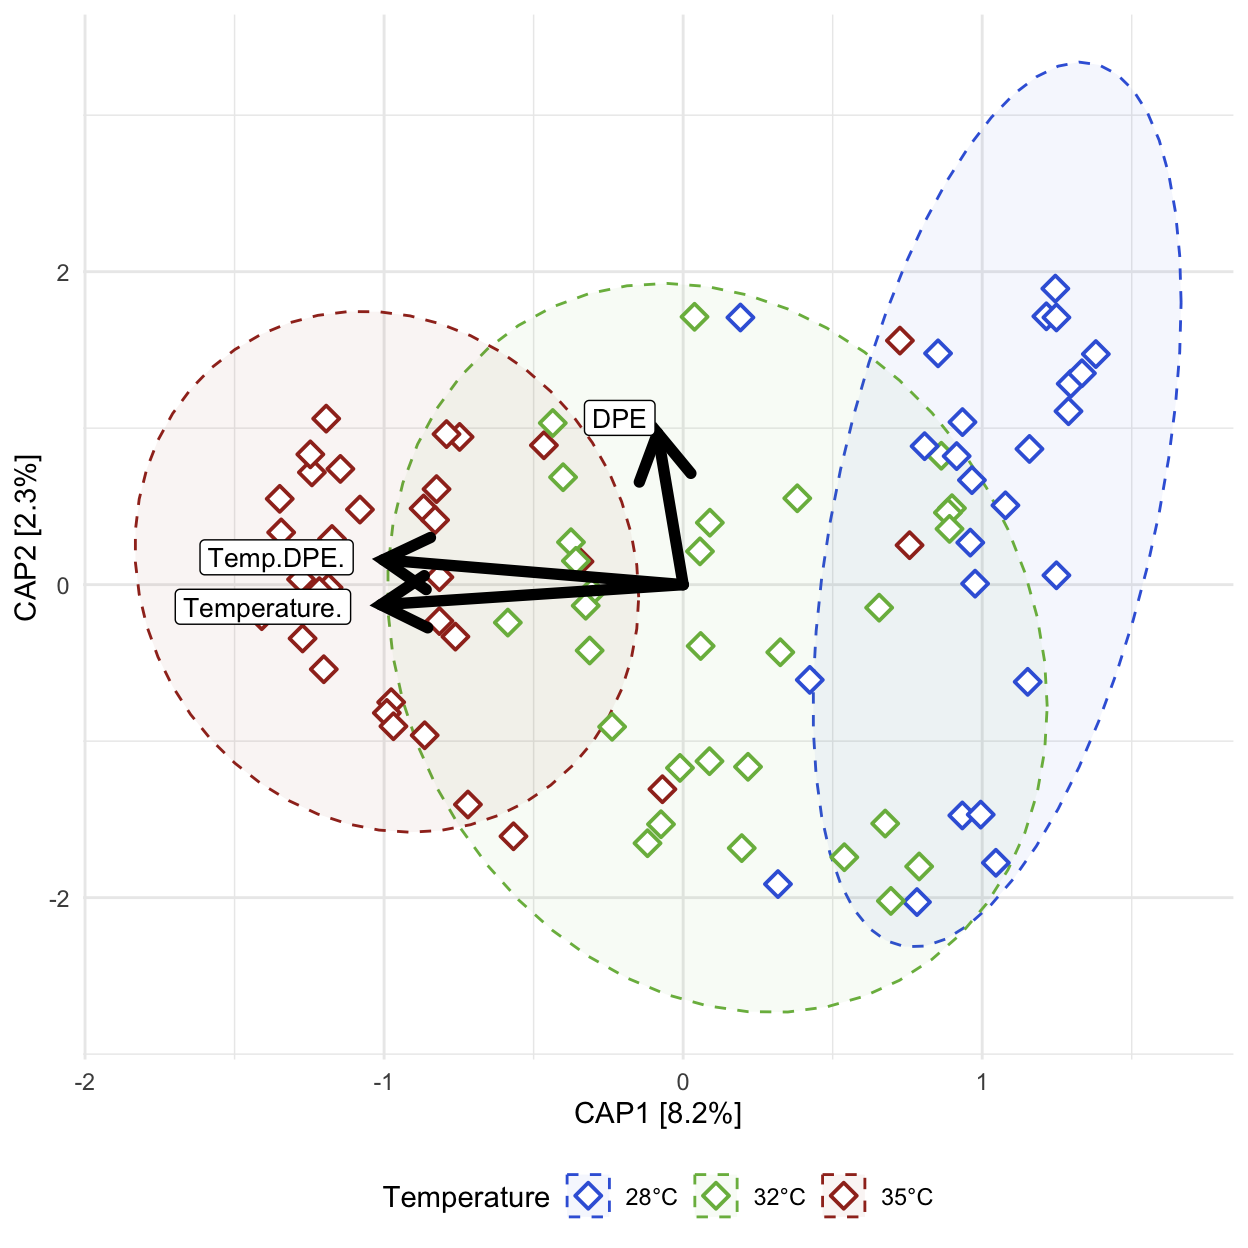
\includegraphics[keepaspectratio]{Results_Overview_files/figure-latex/plots-4D-1.pdf}}

\subparagraph{Tables}\label{tables-10}

(hide)

Click on tabs to display tables. Scroll to see additional rows.

ADONIS2

\begin{longtable}{lrrrrrl}
\caption*{
{\large ADONIS2} \\ 
{\small adonis2(Beta Distance \textasciitilde{} Temperature*DPE); Exposed fish}
} \\ 
\toprule
term & df & SumOfSqs & R2 & statistic & p.value & sig \\ 
\midrule\addlinespace[2.5pt]
\multicolumn{7}{l}{bray} \\ 
\midrule\addlinespace[2.5pt]
Temperature & $2.000$ & $5.218$ & $0.251$ & $14.843$ & $0.001$ & *** \\ 
DPE & $1.000$ & $0.394$ & $0.019$ & $2.241$ & $0.056$ & ns \\ 
Temperature:DPE & $2.000$ & $0.548$ & $0.026$ & $1.558$ & $0.113$ & ns \\ 
Residual & $83.000$ & $14.589$ & $0.703$ & NA & NA & NA \\ 
Total & $88.000$ & $20.748$ & $1.000$ & NA & NA & NA \\ 
\midrule\addlinespace[2.5pt]
\multicolumn{7}{l}{canberra} \\ 
\midrule\addlinespace[2.5pt]
Temperature & $2.000$ & $3.573$ & $0.117$ & $5.847$ & $0.001$ & *** \\ 
DPE & $1.000$ & $0.674$ & $0.022$ & $2.207$ & $0.006$ & ** \\ 
Temperature:DPE & $2.000$ & $0.913$ & $0.030$ & $1.494$ & $0.017$ & * \\ 
Residual & $83.000$ & $25.360$ & $0.831$ & NA & NA & NA \\ 
Total & $88.000$ & $30.520$ & $1.000$ & NA & NA & NA \\ 
\midrule\addlinespace[2.5pt]
\multicolumn{7}{l}{gunifrac} \\ 
\midrule\addlinespace[2.5pt]
Temperature & $2.000$ & $3.363$ & $0.212$ & $11.847$ & $0.001$ & *** \\ 
DPE & $1.000$ & $0.261$ & $0.016$ & $1.837$ & $0.101$ & ns \\ 
Temperature:DPE & $2.000$ & $0.436$ & $0.028$ & $1.535$ & $0.102$ & ns \\ 
Residual & $83.000$ & $11.781$ & $0.744$ & NA & NA & NA \\ 
Total & $88.000$ & $15.841$ & $1.000$ & NA & NA & NA \\ 
\bottomrule
\end{longtable}

Dispersion (ANOVA)

\begin{longtable}{lrrrrrr}
\caption*{
{\large ANOVA: Homogeneity of Dispersion} \\ 
{\small ANOVA(Beta Disperson \textasciitilde{} Temperature); Exposed fish}
} \\ 
\toprule
term & df & sumsq & meansq & statistic & p.value & sig \\ 
\midrule\addlinespace[2.5pt]
\multicolumn{7}{l}{bray} \\ 
\midrule\addlinespace[2.5pt]
Temp.DPE & $11.000$ & $0.624$ & $0.057$ & $3.261$ & $0.001$ & ** \\ 
Residual & $77.000$ & $1.339$ & $0.017$ & NA & NA & NA \\ 
\midrule\addlinespace[2.5pt]
\multicolumn{7}{l}{canberra} \\ 
\midrule\addlinespace[2.5pt]
Temp.DPE & $11.000$ & $0.316$ & $0.029$ & $2.748$ & $0.005$ & ** \\ 
Residual & $77.000$ & $0.805$ & $0.010$ & NA & NA & NA \\ 
\midrule\addlinespace[2.5pt]
\multicolumn{7}{l}{gunifrac} \\ 
\midrule\addlinespace[2.5pt]
Temp.DPE & $11.000$ & $0.420$ & $0.038$ & $3.232$ & $0.001$ & ** \\ 
Residual & $77.000$ & $0.909$ & $0.012$ & NA & NA & NA \\ 
\bottomrule
\end{longtable}

Dispersion (Tukey)

\begin{longtable}{llllrrrrl}
\caption*{
{\large Tukey: Homogeneity of Dispersion} \\ 
{\small Tukey(Beta Disperson \textasciitilde{} Temperature*DPE); Exposed fish}
} \\ 
\toprule
.y. & term & group1 & group2 & estimate & conf.low & conf.high & adj.p.value & sig \\ 
\midrule\addlinespace[2.5pt]
\multicolumn{9}{l}{bray} \\ 
\midrule\addlinespace[2.5pt]
Distance & Temp.DPE & 28°C\_\_21DPE & 28°C\_\_14DPE & $-0.213$ & $-0.485$ & $0.059$ & $\geq$0.25 & ns \\ 
Distance & Temp.DPE & 28°C\_\_28DPE & 28°C\_\_14DPE & $-0.258$ & $-0.512$ & $-0.005$ & $0.042$ & * \\ 
Distance & Temp.DPE & 28°C\_\_42DPE & 28°C\_\_14DPE & $-0.063$ & $-0.285$ & $0.160$ & $\geq$0.25 & ns \\ 
Distance & Temp.DPE & 32°C\_\_14DPE & 28°C\_\_14DPE & $-0.059$ & $-0.270$ & $0.152$ & $\geq$0.25 & ns \\ 
Distance & Temp.DPE & 32°C\_\_21DPE & 28°C\_\_14DPE & $-0.089$ & $-0.319$ & $0.141$ & $\geq$0.25 & ns \\ 
Distance & Temp.DPE & 32°C\_\_28DPE & 28°C\_\_14DPE & $-0.123$ & $-0.363$ & $0.117$ & $\geq$0.25 & ns \\ 
Distance & Temp.DPE & 32°C\_\_42DPE & 28°C\_\_14DPE & $-0.142$ & $-0.372$ & $0.088$ & $\geq$0.25 & ns \\ 
Distance & Temp.DPE & 35°C\_\_14DPE & 28°C\_\_14DPE & $-0.202$ & $-0.418$ & $0.014$ & $0.090$ & ns \\ 
Distance & Temp.DPE & 35°C\_\_21DPE & 28°C\_\_14DPE & $-0.170$ & $-0.393$ & $0.052$ & $\geq$0.25 & ns \\ 
Distance & Temp.DPE & 35°C\_\_28DPE & 28°C\_\_14DPE & $-0.289$ & $-0.511$ & $-0.067$ & $0.002$ & ** \\ 
Distance & Temp.DPE & 35°C\_\_42DPE & 28°C\_\_14DPE & $-0.192$ & $-0.408$ & $0.024$ & $0.130$ & ns \\ 
Distance & Temp.DPE & 28°C\_\_28DPE & 28°C\_\_21DPE & $-0.046$ & $-0.344$ & $0.253$ & $\geq$0.25 & ns \\ 
Distance & Temp.DPE & 28°C\_\_42DPE & 28°C\_\_21DPE & $0.150$ & $-0.122$ & $0.422$ & $\geq$0.25 & ns \\ 
Distance & Temp.DPE & 32°C\_\_14DPE & 28°C\_\_21DPE & $0.153$ & $-0.110$ & $0.416$ & $\geq$0.25 & ns \\ 
Distance & Temp.DPE & 32°C\_\_21DPE & 28°C\_\_21DPE & $0.124$ & $-0.154$ & $0.403$ & $\geq$0.25 & ns \\ 
Distance & Temp.DPE & 32°C\_\_28DPE & 28°C\_\_21DPE & $0.090$ & $-0.197$ & $0.377$ & $\geq$0.25 & ns \\ 
Distance & Temp.DPE & 32°C\_\_42DPE & 28°C\_\_21DPE & $0.071$ & $-0.208$ & $0.350$ & $\geq$0.25 & ns \\ 
Distance & Temp.DPE & 35°C\_\_14DPE & 28°C\_\_21DPE & $0.011$ & $-0.256$ & $0.278$ & $\geq$0.25 & ns \\ 
Distance & Temp.DPE & 35°C\_\_21DPE & 28°C\_\_21DPE & $0.042$ & $-0.230$ & $0.315$ & $\geq$0.25 & ns \\ 
Distance & Temp.DPE & 35°C\_\_28DPE & 28°C\_\_21DPE & $-0.077$ & $-0.349$ & $0.196$ & $\geq$0.25 & ns \\ 
Distance & Temp.DPE & 35°C\_\_42DPE & 28°C\_\_21DPE & $0.021$ & $-0.246$ & $0.288$ & $\geq$0.25 & ns \\ 
Distance & Temp.DPE & 28°C\_\_42DPE & 28°C\_\_28DPE & $0.196$ & $-0.058$ & $0.449$ & $\geq$0.25 & ns \\ 
Distance & Temp.DPE & 32°C\_\_14DPE & 28°C\_\_28DPE & $0.199$ & $-0.044$ & $0.443$ & $0.220$ & ns \\ 
Distance & Temp.DPE & 32°C\_\_21DPE & 28°C\_\_28DPE & $0.170$ & $-0.091$ & $0.430$ & $\geq$0.25 & ns \\ 
Distance & Temp.DPE & 32°C\_\_28DPE & 28°C\_\_28DPE & $0.136$ & $-0.133$ & $0.405$ & $\geq$0.25 & ns \\ 
Distance & Temp.DPE & 32°C\_\_42DPE & 28°C\_\_28DPE & $0.117$ & $-0.144$ & $0.377$ & $\geq$0.25 & ns \\ 
Distance & Temp.DPE & 35°C\_\_14DPE & 28°C\_\_28DPE & $0.057$ & $-0.191$ & $0.305$ & $\geq$0.25 & ns \\ 
Distance & Temp.DPE & 35°C\_\_21DPE & 28°C\_\_28DPE & $0.088$ & $-0.165$ & $0.341$ & $\geq$0.25 & ns \\ 
Distance & Temp.DPE & 35°C\_\_28DPE & 28°C\_\_28DPE & $-0.031$ & $-0.284$ & $0.222$ & $\geq$0.25 & ns \\ 
Distance & Temp.DPE & 35°C\_\_42DPE & 28°C\_\_28DPE & $0.066$ & $-0.182$ & $0.314$ & $\geq$0.25 & ns \\ 
Distance & Temp.DPE & 32°C\_\_14DPE & 28°C\_\_42DPE & $0.003$ & $-0.207$ & $0.214$ & $\geq$0.25 & ns \\ 
Distance & Temp.DPE & 32°C\_\_21DPE & 28°C\_\_42DPE & $-0.026$ & $-0.256$ & $0.204$ & $\geq$0.25 & ns \\ 
Distance & Temp.DPE & 32°C\_\_28DPE & 28°C\_\_42DPE & $-0.060$ & $-0.300$ & $0.180$ & $\geq$0.25 & ns \\ 
Distance & Temp.DPE & 32°C\_\_42DPE & 28°C\_\_42DPE & $-0.079$ & $-0.309$ & $0.151$ & $\geq$0.25 & ns \\ 
Distance & Temp.DPE & 35°C\_\_14DPE & 28°C\_\_42DPE & $-0.139$ & $-0.355$ & $0.077$ & $\geq$0.25 & ns \\ 
Distance & Temp.DPE & 35°C\_\_21DPE & 28°C\_\_42DPE & $-0.108$ & $-0.330$ & $0.115$ & $\geq$0.25 & ns \\ 
Distance & Temp.DPE & 35°C\_\_28DPE & 28°C\_\_42DPE & $-0.227$ & $-0.449$ & $-0.004$ & $0.042$ & * \\ 
Distance & Temp.DPE & 35°C\_\_42DPE & 28°C\_\_42DPE & $-0.129$ & $-0.345$ & $0.087$ & $\geq$0.25 & ns \\ 
Distance & Temp.DPE & 32°C\_\_21DPE & 32°C\_\_14DPE & $-0.029$ & $-0.248$ & $0.190$ & $\geq$0.25 & ns \\ 
Distance & Temp.DPE & 32°C\_\_28DPE & 32°C\_\_14DPE & $-0.063$ & $-0.293$ & $0.166$ & $\geq$0.25 & ns \\ 
Distance & Temp.DPE & 32°C\_\_42DPE & 32°C\_\_14DPE & $-0.082$ & $-0.301$ & $0.137$ & $\geq$0.25 & ns \\ 
Distance & Temp.DPE & 35°C\_\_14DPE & 32°C\_\_14DPE & $-0.142$ & $-0.347$ & $0.062$ & $\geq$0.25 & ns \\ 
Distance & Temp.DPE & 35°C\_\_21DPE & 32°C\_\_14DPE & $-0.111$ & $-0.322$ & $0.100$ & $\geq$0.25 & ns \\ 
Distance & Temp.DPE & 35°C\_\_28DPE & 32°C\_\_14DPE & $-0.230$ & $-0.441$ & $-0.019$ & $0.021$ & * \\ 
Distance & Temp.DPE & 35°C\_\_42DPE & 32°C\_\_14DPE & $-0.133$ & $-0.337$ & $0.072$ & $\geq$0.25 & ns \\ 
Distance & Temp.DPE & 32°C\_\_28DPE & 32°C\_\_21DPE & $-0.034$ & $-0.281$ & $0.213$ & $\geq$0.25 & ns \\ 
Distance & Temp.DPE & 32°C\_\_42DPE & 32°C\_\_21DPE & $-0.053$ & $-0.291$ & $0.185$ & $\geq$0.25 & ns \\ 
Distance & Temp.DPE & 35°C\_\_14DPE & 32°C\_\_21DPE & $-0.113$ & $-0.337$ & $0.111$ & $\geq$0.25 & ns \\ 
Distance & Temp.DPE & 35°C\_\_21DPE & 32°C\_\_21DPE & $-0.082$ & $-0.312$ & $0.148$ & $\geq$0.25 & ns \\ 
Distance & Temp.DPE & 35°C\_\_28DPE & 32°C\_\_21DPE & $-0.201$ & $-0.431$ & $0.029$ & $0.148$ & ns \\ 
Distance & Temp.DPE & 35°C\_\_42DPE & 32°C\_\_21DPE & $-0.103$ & $-0.327$ & $0.121$ & $\geq$0.25 & ns \\ 
Distance & Temp.DPE & 32°C\_\_42DPE & 32°C\_\_28DPE & $-0.019$ & $-0.266$ & $0.228$ & $\geq$0.25 & ns \\ 
Distance & Temp.DPE & 35°C\_\_14DPE & 32°C\_\_28DPE & $-0.079$ & $-0.313$ & $0.155$ & $\geq$0.25 & ns \\ 
Distance & Temp.DPE & 35°C\_\_21DPE & 32°C\_\_28DPE & $-0.048$ & $-0.288$ & $0.192$ & $\geq$0.25 & ns \\ 
Distance & Temp.DPE & 35°C\_\_28DPE & 32°C\_\_28DPE & $-0.167$ & $-0.407$ & $0.073$ & $\geq$0.25 & ns \\ 
Distance & Temp.DPE & 35°C\_\_42DPE & 32°C\_\_28DPE & $-0.069$ & $-0.304$ & $0.165$ & $\geq$0.25 & ns \\ 
Distance & Temp.DPE & 35°C\_\_14DPE & 32°C\_\_42DPE & $-0.060$ & $-0.284$ & $0.164$ & $\geq$0.25 & ns \\ 
Distance & Temp.DPE & 35°C\_\_21DPE & 32°C\_\_42DPE & $-0.029$ & $-0.259$ & $0.201$ & $\geq$0.25 & ns \\ 
Distance & Temp.DPE & 35°C\_\_28DPE & 32°C\_\_42DPE & $-0.148$ & $-0.378$ & $0.082$ & $\geq$0.25 & ns \\ 
Distance & Temp.DPE & 35°C\_\_42DPE & 32°C\_\_42DPE & $-0.050$ & $-0.274$ & $0.174$ & $\geq$0.25 & ns \\ 
Distance & Temp.DPE & 35°C\_\_21DPE & 35°C\_\_14DPE & $0.031$ & $-0.185$ & $0.247$ & $\geq$0.25 & ns \\ 
Distance & Temp.DPE & 35°C\_\_28DPE & 35°C\_\_14DPE & $-0.088$ & $-0.304$ & $0.128$ & $\geq$0.25 & ns \\ 
Distance & Temp.DPE & 35°C\_\_42DPE & 35°C\_\_14DPE & $0.010$ & $-0.200$ & $0.219$ & $\geq$0.25 & ns \\ 
Distance & Temp.DPE & 35°C\_\_28DPE & 35°C\_\_21DPE & $-0.119$ & $-0.341$ & $0.103$ & $\geq$0.25 & ns \\ 
Distance & Temp.DPE & 35°C\_\_42DPE & 35°C\_\_21DPE & $-0.022$ & $-0.238$ & $0.194$ & $\geq$0.25 & ns \\ 
Distance & Temp.DPE & 35°C\_\_42DPE & 35°C\_\_28DPE & $0.097$ & $-0.119$ & $0.313$ & $\geq$0.25 & ns \\ 
\midrule\addlinespace[2.5pt]
\multicolumn{9}{l}{canberra} \\ 
\midrule\addlinespace[2.5pt]
Distance & Temp.DPE & 28°C\_\_21DPE & 28°C\_\_14DPE & $-0.004$ & $-0.215$ & $0.207$ & $\geq$0.25 & ns \\ 
Distance & Temp.DPE & 28°C\_\_28DPE & 28°C\_\_14DPE & $0.040$ & $-0.156$ & $0.237$ & $\geq$0.25 & ns \\ 
Distance & Temp.DPE & 28°C\_\_42DPE & 28°C\_\_14DPE & $0.059$ & $-0.113$ & $0.232$ & $\geq$0.25 & ns \\ 
Distance & Temp.DPE & 32°C\_\_14DPE & 28°C\_\_14DPE & $-0.043$ & $-0.206$ & $0.121$ & $\geq$0.25 & ns \\ 
Distance & Temp.DPE & 32°C\_\_21DPE & 28°C\_\_14DPE & $-0.044$ & $-0.223$ & $0.134$ & $\geq$0.25 & ns \\ 
Distance & Temp.DPE & 32°C\_\_28DPE & 28°C\_\_14DPE & $-0.102$ & $-0.288$ & $0.084$ & $\geq$0.25 & ns \\ 
Distance & Temp.DPE & 32°C\_\_42DPE & 28°C\_\_14DPE & $-0.084$ & $-0.262$ & $0.095$ & $\geq$0.25 & ns \\ 
Distance & Temp.DPE & 35°C\_\_14DPE & 28°C\_\_14DPE & $-0.097$ & $-0.265$ & $0.070$ & $\geq$0.25 & ns \\ 
Distance & Temp.DPE & 35°C\_\_21DPE & 28°C\_\_14DPE & $-0.097$ & $-0.269$ & $0.075$ & $\geq$0.25 & ns \\ 
Distance & Temp.DPE & 35°C\_\_28DPE & 28°C\_\_14DPE & $-0.142$ & $-0.314$ & $0.031$ & $0.215$ & ns \\ 
Distance & Temp.DPE & 35°C\_\_42DPE & 28°C\_\_14DPE & $-0.103$ & $-0.271$ & $0.064$ & $\geq$0.25 & ns \\ 
Distance & Temp.DPE & 28°C\_\_28DPE & 28°C\_\_21DPE & $0.044$ & $-0.187$ & $0.276$ & $\geq$0.25 & ns \\ 
Distance & Temp.DPE & 28°C\_\_42DPE & 28°C\_\_21DPE & $0.064$ & $-0.148$ & $0.275$ & $\geq$0.25 & ns \\ 
Distance & Temp.DPE & 32°C\_\_14DPE & 28°C\_\_21DPE & $-0.039$ & $-0.243$ & $0.165$ & $\geq$0.25 & ns \\ 
Distance & Temp.DPE & 32°C\_\_21DPE & 28°C\_\_21DPE & $-0.040$ & $-0.256$ & $0.176$ & $\geq$0.25 & ns \\ 
Distance & Temp.DPE & 32°C\_\_28DPE & 28°C\_\_21DPE & $-0.097$ & $-0.320$ & $0.125$ & $\geq$0.25 & ns \\ 
Distance & Temp.DPE & 32°C\_\_42DPE & 28°C\_\_21DPE & $-0.079$ & $-0.295$ & $0.137$ & $\geq$0.25 & ns \\ 
Distance & Temp.DPE & 35°C\_\_14DPE & 28°C\_\_21DPE & $-0.093$ & $-0.300$ & $0.114$ & $\geq$0.25 & ns \\ 
Distance & Temp.DPE & 35°C\_\_21DPE & 28°C\_\_21DPE & $-0.093$ & $-0.304$ & $0.118$ & $\geq$0.25 & ns \\ 
Distance & Temp.DPE & 35°C\_\_28DPE & 28°C\_\_21DPE & $-0.137$ & $-0.348$ & $0.074$ & $\geq$0.25 & ns \\ 
Distance & Temp.DPE & 35°C\_\_42DPE & 28°C\_\_21DPE & $-0.099$ & $-0.306$ & $0.108$ & $\geq$0.25 & ns \\ 
Distance & Temp.DPE & 28°C\_\_42DPE & 28°C\_\_28DPE & $0.019$ & $-0.177$ & $0.216$ & $\geq$0.25 & ns \\ 
Distance & Temp.DPE & 32°C\_\_14DPE & 28°C\_\_28DPE & $-0.083$ & $-0.272$ & $0.106$ & $\geq$0.25 & ns \\ 
Distance & Temp.DPE & 32°C\_\_21DPE & 28°C\_\_28DPE & $-0.085$ & $-0.286$ & $0.117$ & $\geq$0.25 & ns \\ 
Distance & Temp.DPE & 32°C\_\_28DPE & 28°C\_\_28DPE & $-0.142$ & $-0.351$ & $0.067$ & $\geq$0.25 & ns \\ 
Distance & Temp.DPE & 32°C\_\_42DPE & 28°C\_\_28DPE & $-0.124$ & $-0.326$ & $0.078$ & $\geq$0.25 & ns \\ 
Distance & Temp.DPE & 35°C\_\_14DPE & 28°C\_\_28DPE & $-0.137$ & $-0.329$ & $0.055$ & $\geq$0.25 & ns \\ 
Distance & Temp.DPE & 35°C\_\_21DPE & 28°C\_\_28DPE & $-0.137$ & $-0.334$ & $0.059$ & $\geq$0.25 & ns \\ 
Distance & Temp.DPE & 35°C\_\_28DPE & 28°C\_\_28DPE & $-0.182$ & $-0.378$ & $0.015$ & $0.097$ & ns \\ 
Distance & Temp.DPE & 35°C\_\_42DPE & 28°C\_\_28DPE & $-0.144$ & $-0.336$ & $0.049$ & $\geq$0.25 & ns \\ 
Distance & Temp.DPE & 32°C\_\_14DPE & 28°C\_\_42DPE & $-0.102$ & $-0.266$ & $0.061$ & $\geq$0.25 & ns \\ 
Distance & Temp.DPE & 32°C\_\_21DPE & 28°C\_\_42DPE & $-0.104$ & $-0.282$ & $0.075$ & $\geq$0.25 & ns \\ 
Distance & Temp.DPE & 32°C\_\_28DPE & 28°C\_\_42DPE & $-0.161$ & $-0.347$ & $0.025$ & $0.157$ & ns \\ 
Distance & Temp.DPE & 32°C\_\_42DPE & 28°C\_\_42DPE & $-0.143$ & $-0.321$ & $0.036$ & $0.247$ & ns \\ 
Distance & Temp.DPE & 35°C\_\_14DPE & 28°C\_\_42DPE & $-0.156$ & $-0.324$ & $0.011$ & $0.091$ & ns \\ 
Distance & Temp.DPE & 35°C\_\_21DPE & 28°C\_\_42DPE & $-0.156$ & $-0.329$ & $0.016$ & $0.112$ & ns \\ 
Distance & Temp.DPE & 35°C\_\_28DPE & 28°C\_\_42DPE & $-0.201$ & $-0.373$ & $-0.028$ & $0.010$ & ** \\ 
Distance & Temp.DPE & 35°C\_\_42DPE & 28°C\_\_42DPE & $-0.163$ & $-0.330$ & $0.005$ & $0.065$ & ns \\ 
Distance & Temp.DPE & 32°C\_\_21DPE & 32°C\_\_14DPE & $-0.001$ & $-0.171$ & $0.168$ & $\geq$0.25 & ns \\ 
Distance & Temp.DPE & 32°C\_\_28DPE & 32°C\_\_14DPE & $-0.059$ & $-0.237$ & $0.119$ & $\geq$0.25 & ns \\ 
Distance & Temp.DPE & 32°C\_\_42DPE & 32°C\_\_14DPE & $-0.041$ & $-0.211$ & $0.129$ & $\geq$0.25 & ns \\ 
Distance & Temp.DPE & 35°C\_\_14DPE & 32°C\_\_14DPE & $-0.054$ & $-0.212$ & $0.104$ & $\geq$0.25 & ns \\ 
Distance & Temp.DPE & 35°C\_\_21DPE & 32°C\_\_14DPE & $-0.054$ & $-0.218$ & $0.109$ & $\geq$0.25 & ns \\ 
Distance & Temp.DPE & 35°C\_\_28DPE & 32°C\_\_14DPE & $-0.099$ & $-0.262$ & $0.065$ & $\geq$0.25 & ns \\ 
Distance & Temp.DPE & 35°C\_\_42DPE & 32°C\_\_14DPE & $-0.060$ & $-0.219$ & $0.098$ & $\geq$0.25 & ns \\ 
Distance & Temp.DPE & 32°C\_\_28DPE & 32°C\_\_21DPE & $-0.057$ & $-0.249$ & $0.134$ & $\geq$0.25 & ns \\ 
Distance & Temp.DPE & 32°C\_\_42DPE & 32°C\_\_21DPE & $-0.039$ & $-0.224$ & $0.145$ & $\geq$0.25 & ns \\ 
Distance & Temp.DPE & 35°C\_\_14DPE & 32°C\_\_21DPE & $-0.053$ & $-0.226$ & $0.121$ & $\geq$0.25 & ns \\ 
Distance & Temp.DPE & 35°C\_\_21DPE & 32°C\_\_21DPE & $-0.053$ & $-0.231$ & $0.126$ & $\geq$0.25 & ns \\ 
Distance & Temp.DPE & 35°C\_\_28DPE & 32°C\_\_21DPE & $-0.097$ & $-0.276$ & $0.081$ & $\geq$0.25 & ns \\ 
Distance & Temp.DPE & 35°C\_\_42DPE & 32°C\_\_21DPE & $-0.059$ & $-0.233$ & $0.115$ & $\geq$0.25 & ns \\ 
Distance & Temp.DPE & 32°C\_\_42DPE & 32°C\_\_28DPE & $0.018$ & $-0.174$ & $0.210$ & $\geq$0.25 & ns \\ 
Distance & Temp.DPE & 35°C\_\_14DPE & 32°C\_\_28DPE & $0.005$ & $-0.177$ & $0.186$ & $\geq$0.25 & ns \\ 
Distance & Temp.DPE & 35°C\_\_21DPE & 32°C\_\_28DPE & $0.005$ & $-0.182$ & $0.191$ & $\geq$0.25 & ns \\ 
Distance & Temp.DPE & 35°C\_\_28DPE & 32°C\_\_28DPE & $-0.040$ & $-0.226$ & $0.146$ & $\geq$0.25 & ns \\ 
Distance & Temp.DPE & 35°C\_\_42DPE & 32°C\_\_28DPE & $-0.002$ & $-0.183$ & $0.180$ & $\geq$0.25 & ns \\ 
Distance & Temp.DPE & 35°C\_\_14DPE & 32°C\_\_42DPE & $-0.013$ & $-0.187$ & $0.160$ & $\geq$0.25 & ns \\ 
Distance & Temp.DPE & 35°C\_\_21DPE & 32°C\_\_42DPE & $-0.014$ & $-0.192$ & $0.165$ & $\geq$0.25 & ns \\ 
Distance & Temp.DPE & 35°C\_\_28DPE & 32°C\_\_42DPE & $-0.058$ & $-0.236$ & $0.120$ & $\geq$0.25 & ns \\ 
Distance & Temp.DPE & 35°C\_\_42DPE & 32°C\_\_42DPE & $-0.020$ & $-0.194$ & $0.154$ & $\geq$0.25 & ns \\ 
Distance & Temp.DPE & 35°C\_\_21DPE & 35°C\_\_14DPE & $0.000$ & $-0.168$ & $0.167$ & $\geq$0.25 & ns \\ 
Distance & Temp.DPE & 35°C\_\_28DPE & 35°C\_\_14DPE & $-0.044$ & $-0.212$ & $0.123$ & $\geq$0.25 & ns \\ 
Distance & Temp.DPE & 35°C\_\_42DPE & 35°C\_\_14DPE & $-0.006$ & $-0.169$ & $0.156$ & $\geq$0.25 & ns \\ 
Distance & Temp.DPE & 35°C\_\_28DPE & 35°C\_\_21DPE & $-0.044$ & $-0.217$ & $0.128$ & $\geq$0.25 & ns \\ 
Distance & Temp.DPE & 35°C\_\_42DPE & 35°C\_\_21DPE & $-0.006$ & $-0.174$ & $0.161$ & $\geq$0.25 & ns \\ 
Distance & Temp.DPE & 35°C\_\_42DPE & 35°C\_\_28DPE & $0.038$ & $-0.129$ & $0.206$ & $\geq$0.25 & ns \\ 
\midrule\addlinespace[2.5pt]
\multicolumn{9}{l}{gunifrac} \\ 
\midrule\addlinespace[2.5pt]
Distance & Temp.DPE & 28°C\_\_21DPE & 28°C\_\_14DPE & $-0.191$ & $-0.415$ & $0.033$ & $0.173$ & ns \\ 
Distance & Temp.DPE & 28°C\_\_28DPE & 28°C\_\_14DPE & $-0.061$ & $-0.270$ & $0.147$ & $\geq$0.25 & ns \\ 
Distance & Temp.DPE & 28°C\_\_42DPE & 28°C\_\_14DPE & $0.018$ & $-0.165$ & $0.201$ & $\geq$0.25 & ns \\ 
Distance & Temp.DPE & 32°C\_\_14DPE & 28°C\_\_14DPE & $-0.024$ & $-0.197$ & $0.150$ & $\geq$0.25 & ns \\ 
Distance & Temp.DPE & 32°C\_\_21DPE & 28°C\_\_14DPE & $-0.027$ & $-0.216$ & $0.163$ & $\geq$0.25 & ns \\ 
Distance & Temp.DPE & 32°C\_\_28DPE & 28°C\_\_14DPE & $-0.100$ & $-0.298$ & $0.098$ & $\geq$0.25 & ns \\ 
Distance & Temp.DPE & 32°C\_\_42DPE & 28°C\_\_14DPE & $-0.069$ & $-0.259$ & $0.120$ & $\geq$0.25 & ns \\ 
Distance & Temp.DPE & 35°C\_\_14DPE & 28°C\_\_14DPE & $-0.131$ & $-0.309$ & $0.047$ & $\geq$0.25 & ns \\ 
Distance & Temp.DPE & 35°C\_\_21DPE & 28°C\_\_14DPE & $-0.137$ & $-0.320$ & $0.046$ & $\geq$0.25 & ns \\ 
Distance & Temp.DPE & 35°C\_\_28DPE & 28°C\_\_14DPE & $-0.198$ & $-0.382$ & $-0.015$ & $0.022$ & * \\ 
Distance & Temp.DPE & 35°C\_\_42DPE & 28°C\_\_14DPE & $-0.134$ & $-0.312$ & $0.044$ & $\geq$0.25 & ns \\ 
Distance & Temp.DPE & 28°C\_\_28DPE & 28°C\_\_21DPE & $0.130$ & $-0.116$ & $0.375$ & $\geq$0.25 & ns \\ 
Distance & Temp.DPE & 28°C\_\_42DPE & 28°C\_\_21DPE & $0.209$ & $-0.015$ & $0.433$ & $0.092$ & ns \\ 
Distance & Temp.DPE & 32°C\_\_14DPE & 28°C\_\_21DPE & $0.167$ & $-0.049$ & $0.384$ & $\geq$0.25 & ns \\ 
Distance & Temp.DPE & 32°C\_\_21DPE & 28°C\_\_21DPE & $0.164$ & $-0.065$ & $0.394$ & $\geq$0.25 & ns \\ 
Distance & Temp.DPE & 32°C\_\_28DPE & 28°C\_\_21DPE & $0.091$ & $-0.146$ & $0.327$ & $\geq$0.25 & ns \\ 
Distance & Temp.DPE & 32°C\_\_42DPE & 28°C\_\_21DPE & $0.122$ & $-0.108$ & $0.351$ & $\geq$0.25 & ns \\ 
Distance & Temp.DPE & 35°C\_\_14DPE & 28°C\_\_21DPE & $0.060$ & $-0.161$ & $0.280$ & $\geq$0.25 & ns \\ 
Distance & Temp.DPE & 35°C\_\_21DPE & 28°C\_\_21DPE & $0.054$ & $-0.170$ & $0.278$ & $\geq$0.25 & ns \\ 
Distance & Temp.DPE & 35°C\_\_28DPE & 28°C\_\_21DPE & $-0.007$ & $-0.232$ & $0.217$ & $\geq$0.25 & ns \\ 
Distance & Temp.DPE & 35°C\_\_42DPE & 28°C\_\_21DPE & $0.057$ & $-0.163$ & $0.277$ & $\geq$0.25 & ns \\ 
Distance & Temp.DPE & 28°C\_\_42DPE & 28°C\_\_28DPE & $0.079$ & $-0.130$ & $0.288$ & $\geq$0.25 & ns \\ 
Distance & Temp.DPE & 32°C\_\_14DPE & 28°C\_\_28DPE & $0.038$ & $-0.163$ & $0.238$ & $\geq$0.25 & ns \\ 
Distance & Temp.DPE & 32°C\_\_21DPE & 28°C\_\_28DPE & $0.035$ & $-0.180$ & $0.249$ & $\geq$0.25 & ns \\ 
Distance & Temp.DPE & 32°C\_\_28DPE & 28°C\_\_28DPE & $-0.039$ & $-0.260$ & $0.183$ & $\geq$0.25 & ns \\ 
Distance & Temp.DPE & 32°C\_\_42DPE & 28°C\_\_28DPE & $-0.008$ & $-0.222$ & $0.206$ & $\geq$0.25 & ns \\ 
Distance & Temp.DPE & 35°C\_\_14DPE & 28°C\_\_28DPE & $-0.070$ & $-0.274$ & $0.134$ & $\geq$0.25 & ns \\ 
Distance & Temp.DPE & 35°C\_\_21DPE & 28°C\_\_28DPE & $-0.075$ & $-0.284$ & $0.133$ & $\geq$0.25 & ns \\ 
Distance & Temp.DPE & 35°C\_\_28DPE & 28°C\_\_28DPE & $-0.137$ & $-0.346$ & $0.072$ & $\geq$0.25 & ns \\ 
Distance & Temp.DPE & 35°C\_\_42DPE & 28°C\_\_28DPE & $-0.072$ & $-0.277$ & $0.132$ & $\geq$0.25 & ns \\ 
Distance & Temp.DPE & 32°C\_\_14DPE & 28°C\_\_42DPE & $-0.041$ & $-0.215$ & $0.132$ & $\geq$0.25 & ns \\ 
Distance & Temp.DPE & 32°C\_\_21DPE & 28°C\_\_42DPE & $-0.045$ & $-0.234$ & $0.145$ & $\geq$0.25 & ns \\ 
Distance & Temp.DPE & 32°C\_\_28DPE & 28°C\_\_42DPE & $-0.118$ & $-0.316$ & $0.080$ & $\geq$0.25 & ns \\ 
Distance & Temp.DPE & 32°C\_\_42DPE & 28°C\_\_42DPE & $-0.087$ & $-0.277$ & $0.102$ & $\geq$0.25 & ns \\ 
Distance & Temp.DPE & 35°C\_\_14DPE & 28°C\_\_42DPE & $-0.149$ & $-0.327$ & $0.029$ & $0.190$ & ns \\ 
Distance & Temp.DPE & 35°C\_\_21DPE & 28°C\_\_42DPE & $-0.155$ & $-0.338$ & $0.029$ & $0.182$ & ns \\ 
Distance & Temp.DPE & 35°C\_\_28DPE & 28°C\_\_42DPE & $-0.216$ & $-0.399$ & $-0.033$ & $0.008$ & ** \\ 
Distance & Temp.DPE & 35°C\_\_42DPE & 28°C\_\_42DPE & $-0.151$ & $-0.329$ & $0.026$ & $0.173$ & ns \\ 
Distance & Temp.DPE & 32°C\_\_21DPE & 32°C\_\_14DPE & $-0.003$ & $-0.184$ & $0.177$ & $\geq$0.25 & ns \\ 
Distance & Temp.DPE & 32°C\_\_28DPE & 32°C\_\_14DPE & $-0.076$ & $-0.266$ & $0.113$ & $\geq$0.25 & ns \\ 
Distance & Temp.DPE & 32°C\_\_42DPE & 32°C\_\_14DPE & $-0.046$ & $-0.226$ & $0.135$ & $\geq$0.25 & ns \\ 
Distance & Temp.DPE & 35°C\_\_14DPE & 32°C\_\_14DPE & $-0.108$ & $-0.276$ & $0.060$ & $\geq$0.25 & ns \\ 
Distance & Temp.DPE & 35°C\_\_21DPE & 32°C\_\_14DPE & $-0.113$ & $-0.287$ & $0.061$ & $\geq$0.25 & ns \\ 
Distance & Temp.DPE & 35°C\_\_28DPE & 32°C\_\_14DPE & $-0.175$ & $-0.348$ & $-0.001$ & $0.047$ & * \\ 
Distance & Temp.DPE & 35°C\_\_42DPE & 32°C\_\_14DPE & $-0.110$ & $-0.278$ & $0.058$ & $\geq$0.25 & ns \\ 
Distance & Temp.DPE & 32°C\_\_28DPE & 32°C\_\_21DPE & $-0.073$ & $-0.277$ & $0.130$ & $\geq$0.25 & ns \\ 
Distance & Temp.DPE & 32°C\_\_42DPE & 32°C\_\_21DPE & $-0.043$ & $-0.238$ & $0.153$ & $\geq$0.25 & ns \\ 
Distance & Temp.DPE & 35°C\_\_14DPE & 32°C\_\_21DPE & $-0.105$ & $-0.289$ & $0.080$ & $\geq$0.25 & ns \\ 
Distance & Temp.DPE & 35°C\_\_21DPE & 32°C\_\_21DPE & $-0.110$ & $-0.300$ & $0.079$ & $\geq$0.25 & ns \\ 
Distance & Temp.DPE & 35°C\_\_28DPE & 32°C\_\_21DPE & $-0.172$ & $-0.361$ & $0.018$ & $0.113$ & ns \\ 
Distance & Temp.DPE & 35°C\_\_42DPE & 32°C\_\_21DPE & $-0.107$ & $-0.292$ & $0.078$ & $\geq$0.25 & ns \\ 
Distance & Temp.DPE & 32°C\_\_42DPE & 32°C\_\_28DPE & $0.031$ & $-0.173$ & $0.234$ & $\geq$0.25 & ns \\ 
Distance & Temp.DPE & 35°C\_\_14DPE & 32°C\_\_28DPE & $-0.031$ & $-0.224$ & $0.162$ & $\geq$0.25 & ns \\ 
Distance & Temp.DPE & 35°C\_\_21DPE & 32°C\_\_28DPE & $-0.037$ & $-0.234$ & $0.161$ & $\geq$0.25 & ns \\ 
Distance & Temp.DPE & 35°C\_\_28DPE & 32°C\_\_28DPE & $-0.098$ & $-0.296$ & $0.099$ & $\geq$0.25 & ns \\ 
Distance & Temp.DPE & 35°C\_\_42DPE & 32°C\_\_28DPE & $-0.034$ & $-0.227$ & $0.159$ & $\geq$0.25 & ns \\ 
Distance & Temp.DPE & 35°C\_\_14DPE & 32°C\_\_42DPE & $-0.062$ & $-0.247$ & $0.122$ & $\geq$0.25 & ns \\ 
Distance & Temp.DPE & 35°C\_\_21DPE & 32°C\_\_42DPE & $-0.067$ & $-0.257$ & $0.122$ & $\geq$0.25 & ns \\ 
Distance & Temp.DPE & 35°C\_\_28DPE & 32°C\_\_42DPE & $-0.129$ & $-0.319$ & $0.060$ & $\geq$0.25 & ns \\ 
Distance & Temp.DPE & 35°C\_\_42DPE & 32°C\_\_42DPE & $-0.064$ & $-0.249$ & $0.120$ & $\geq$0.25 & ns \\ 
Distance & Temp.DPE & 35°C\_\_21DPE & 35°C\_\_14DPE & $-0.005$ & $-0.183$ & $0.173$ & $\geq$0.25 & ns \\ 
Distance & Temp.DPE & 35°C\_\_28DPE & 35°C\_\_14DPE & $-0.067$ & $-0.245$ & $0.111$ & $\geq$0.25 & ns \\ 
Distance & Temp.DPE & 35°C\_\_42DPE & 35°C\_\_14DPE & $-0.002$ & $-0.175$ & $0.170$ & $\geq$0.25 & ns \\ 
Distance & Temp.DPE & 35°C\_\_28DPE & 35°C\_\_21DPE & $-0.062$ & $-0.245$ & $0.121$ & $\geq$0.25 & ns \\ 
Distance & Temp.DPE & 35°C\_\_42DPE & 35°C\_\_21DPE & $0.003$ & $-0.175$ & $0.181$ & $\geq$0.25 & ns \\ 
Distance & Temp.DPE & 35°C\_\_42DPE & 35°C\_\_28DPE & $0.065$ & $-0.113$ & $0.243$ & $\geq$0.25 & ns \\ 
\bottomrule
\end{longtable}

\subparagraph{Addl. Metrics}\label{addl.-metrics-7}

\subsubsection{}\label{section-2}

\paragraph{(hide)}\label{hide-13}

Click on tabs to reveal figures displaying additional metrics.

\paragraph{S4A}\label{s4a}

\pandocbounded{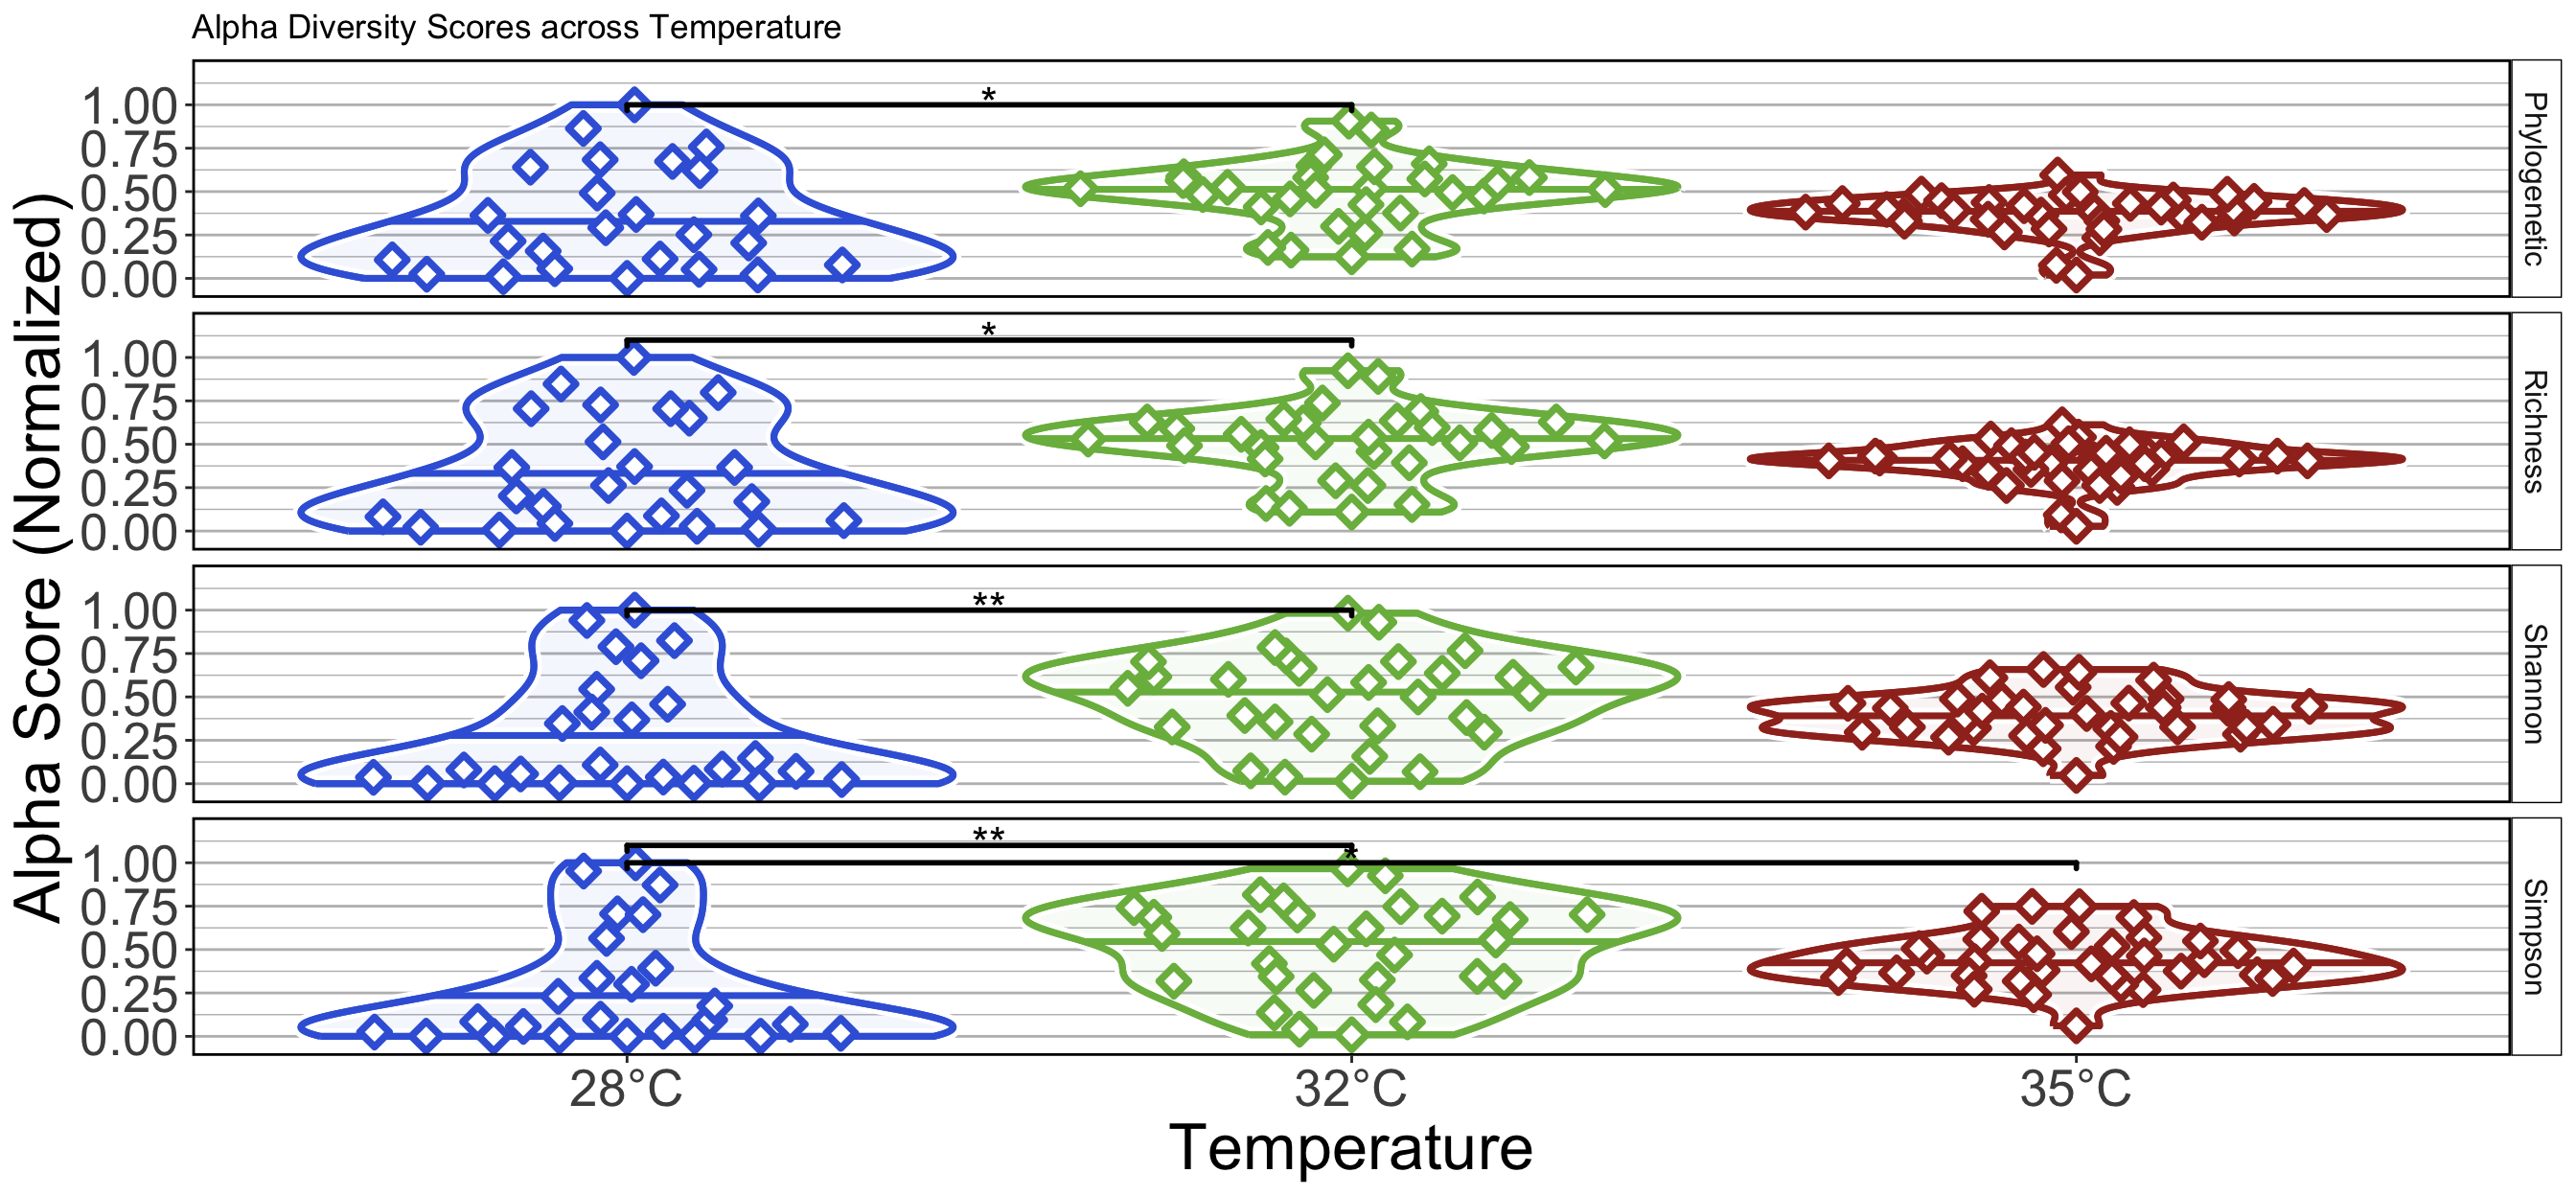
\includegraphics[keepaspectratio]{Results_Overview_files/figure-latex/plots-S4A-1.pdf}}

\paragraph{S4B}\label{s4b}

\pandocbounded{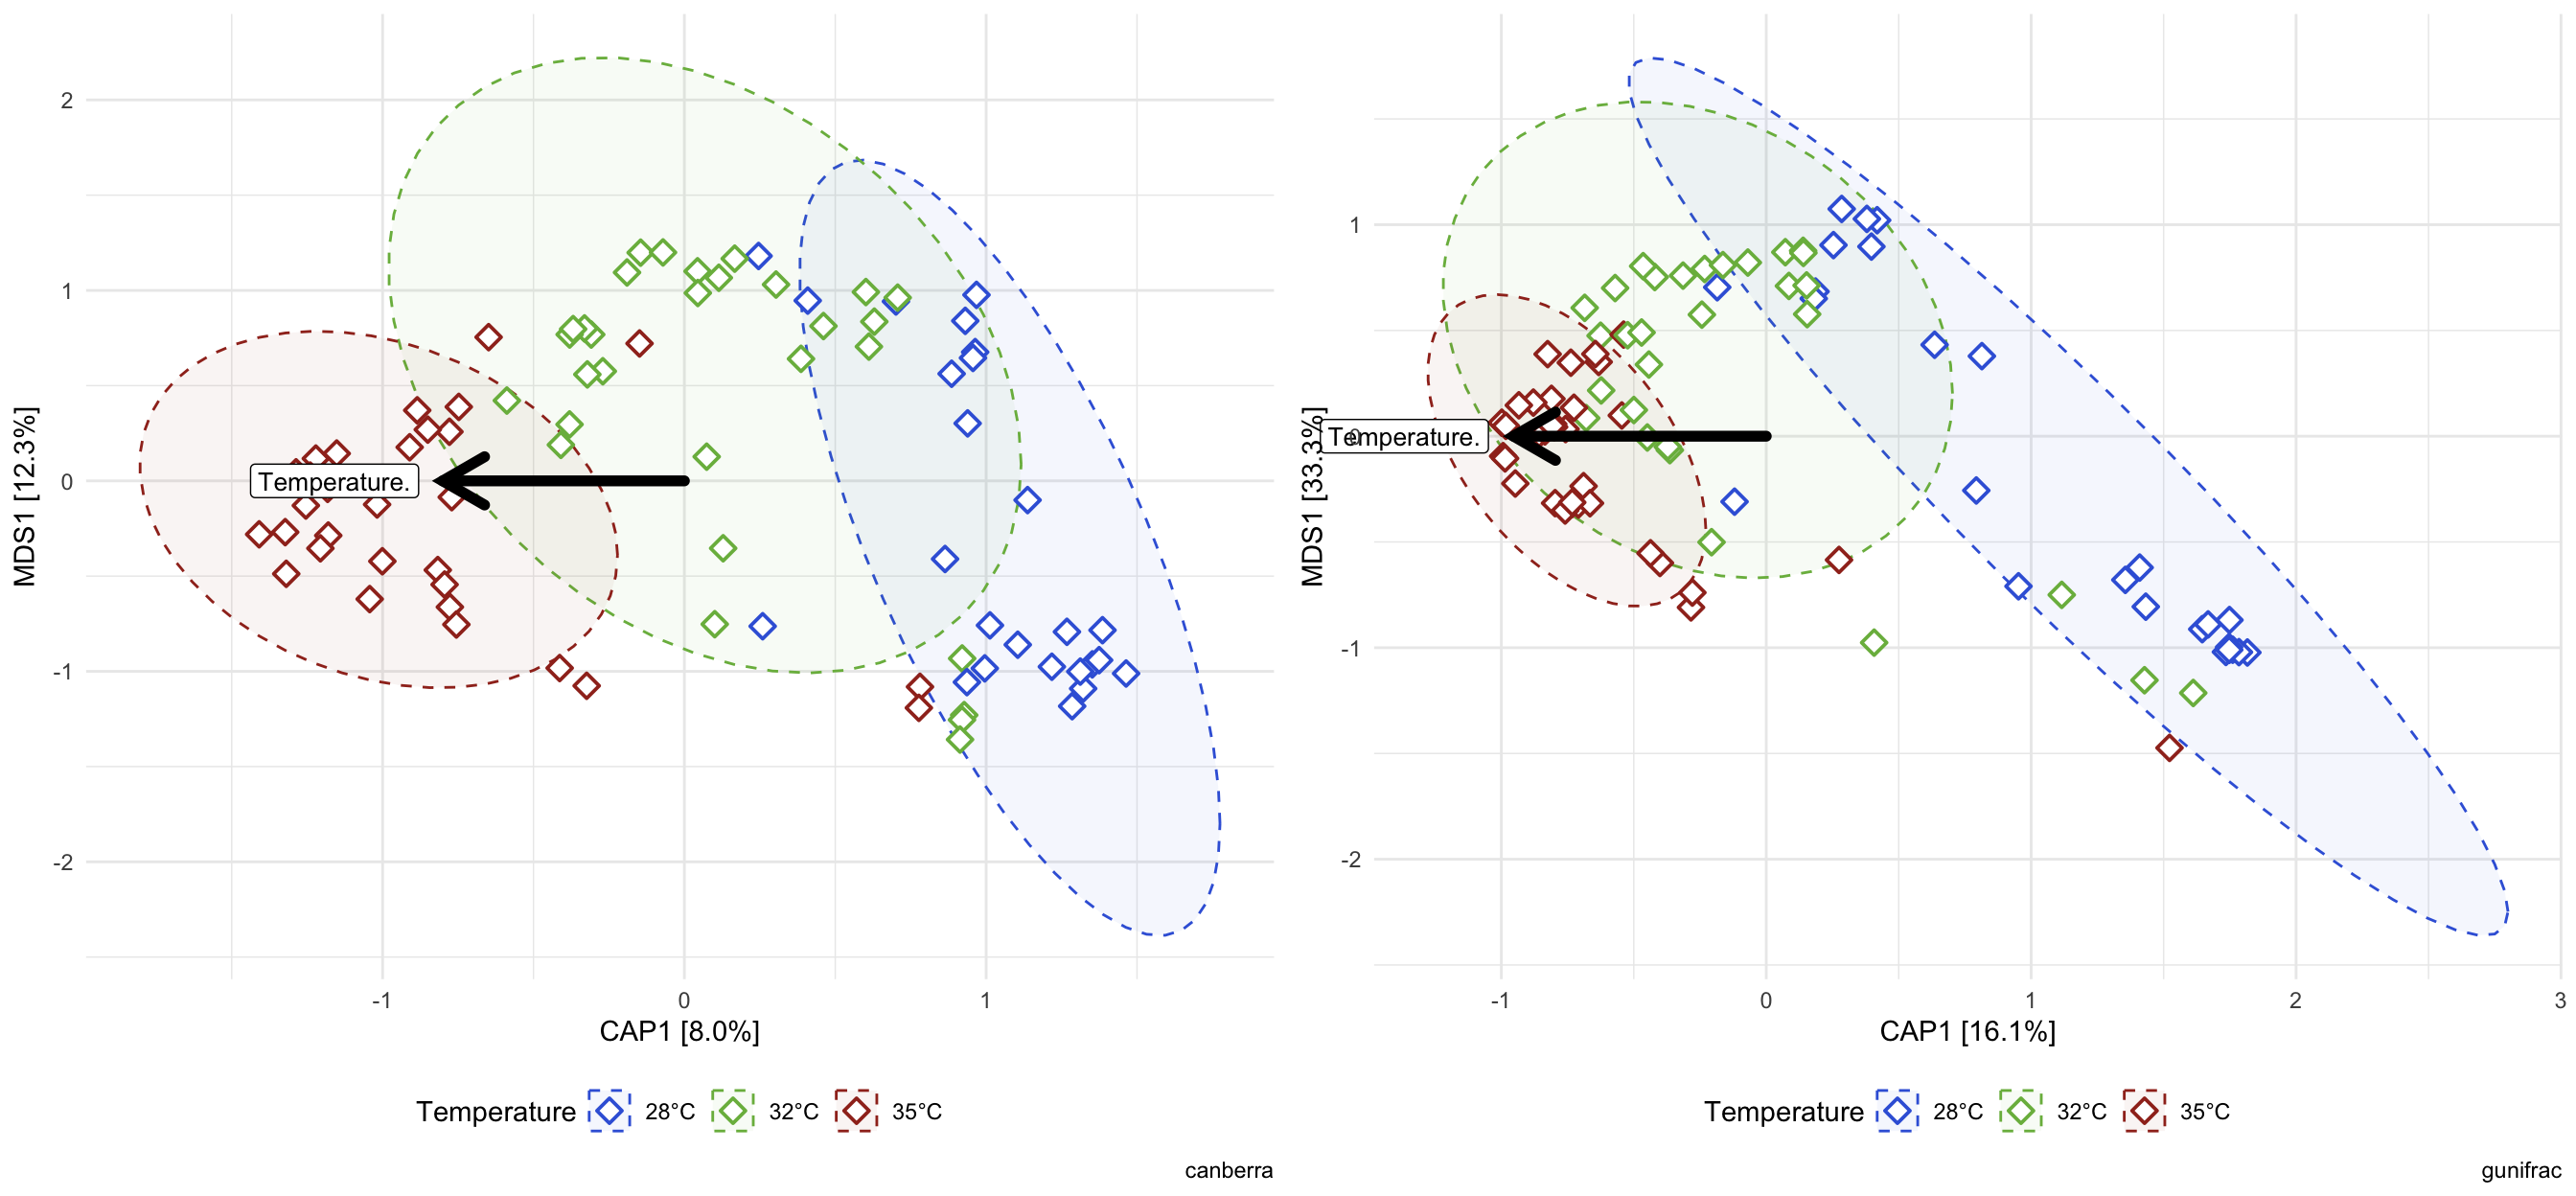
\includegraphics[keepaspectratio]{Results_Overview_files/figure-latex/plots-S4B-1.pdf}}

\paragraph{S4C}\label{s4c}

\pandocbounded{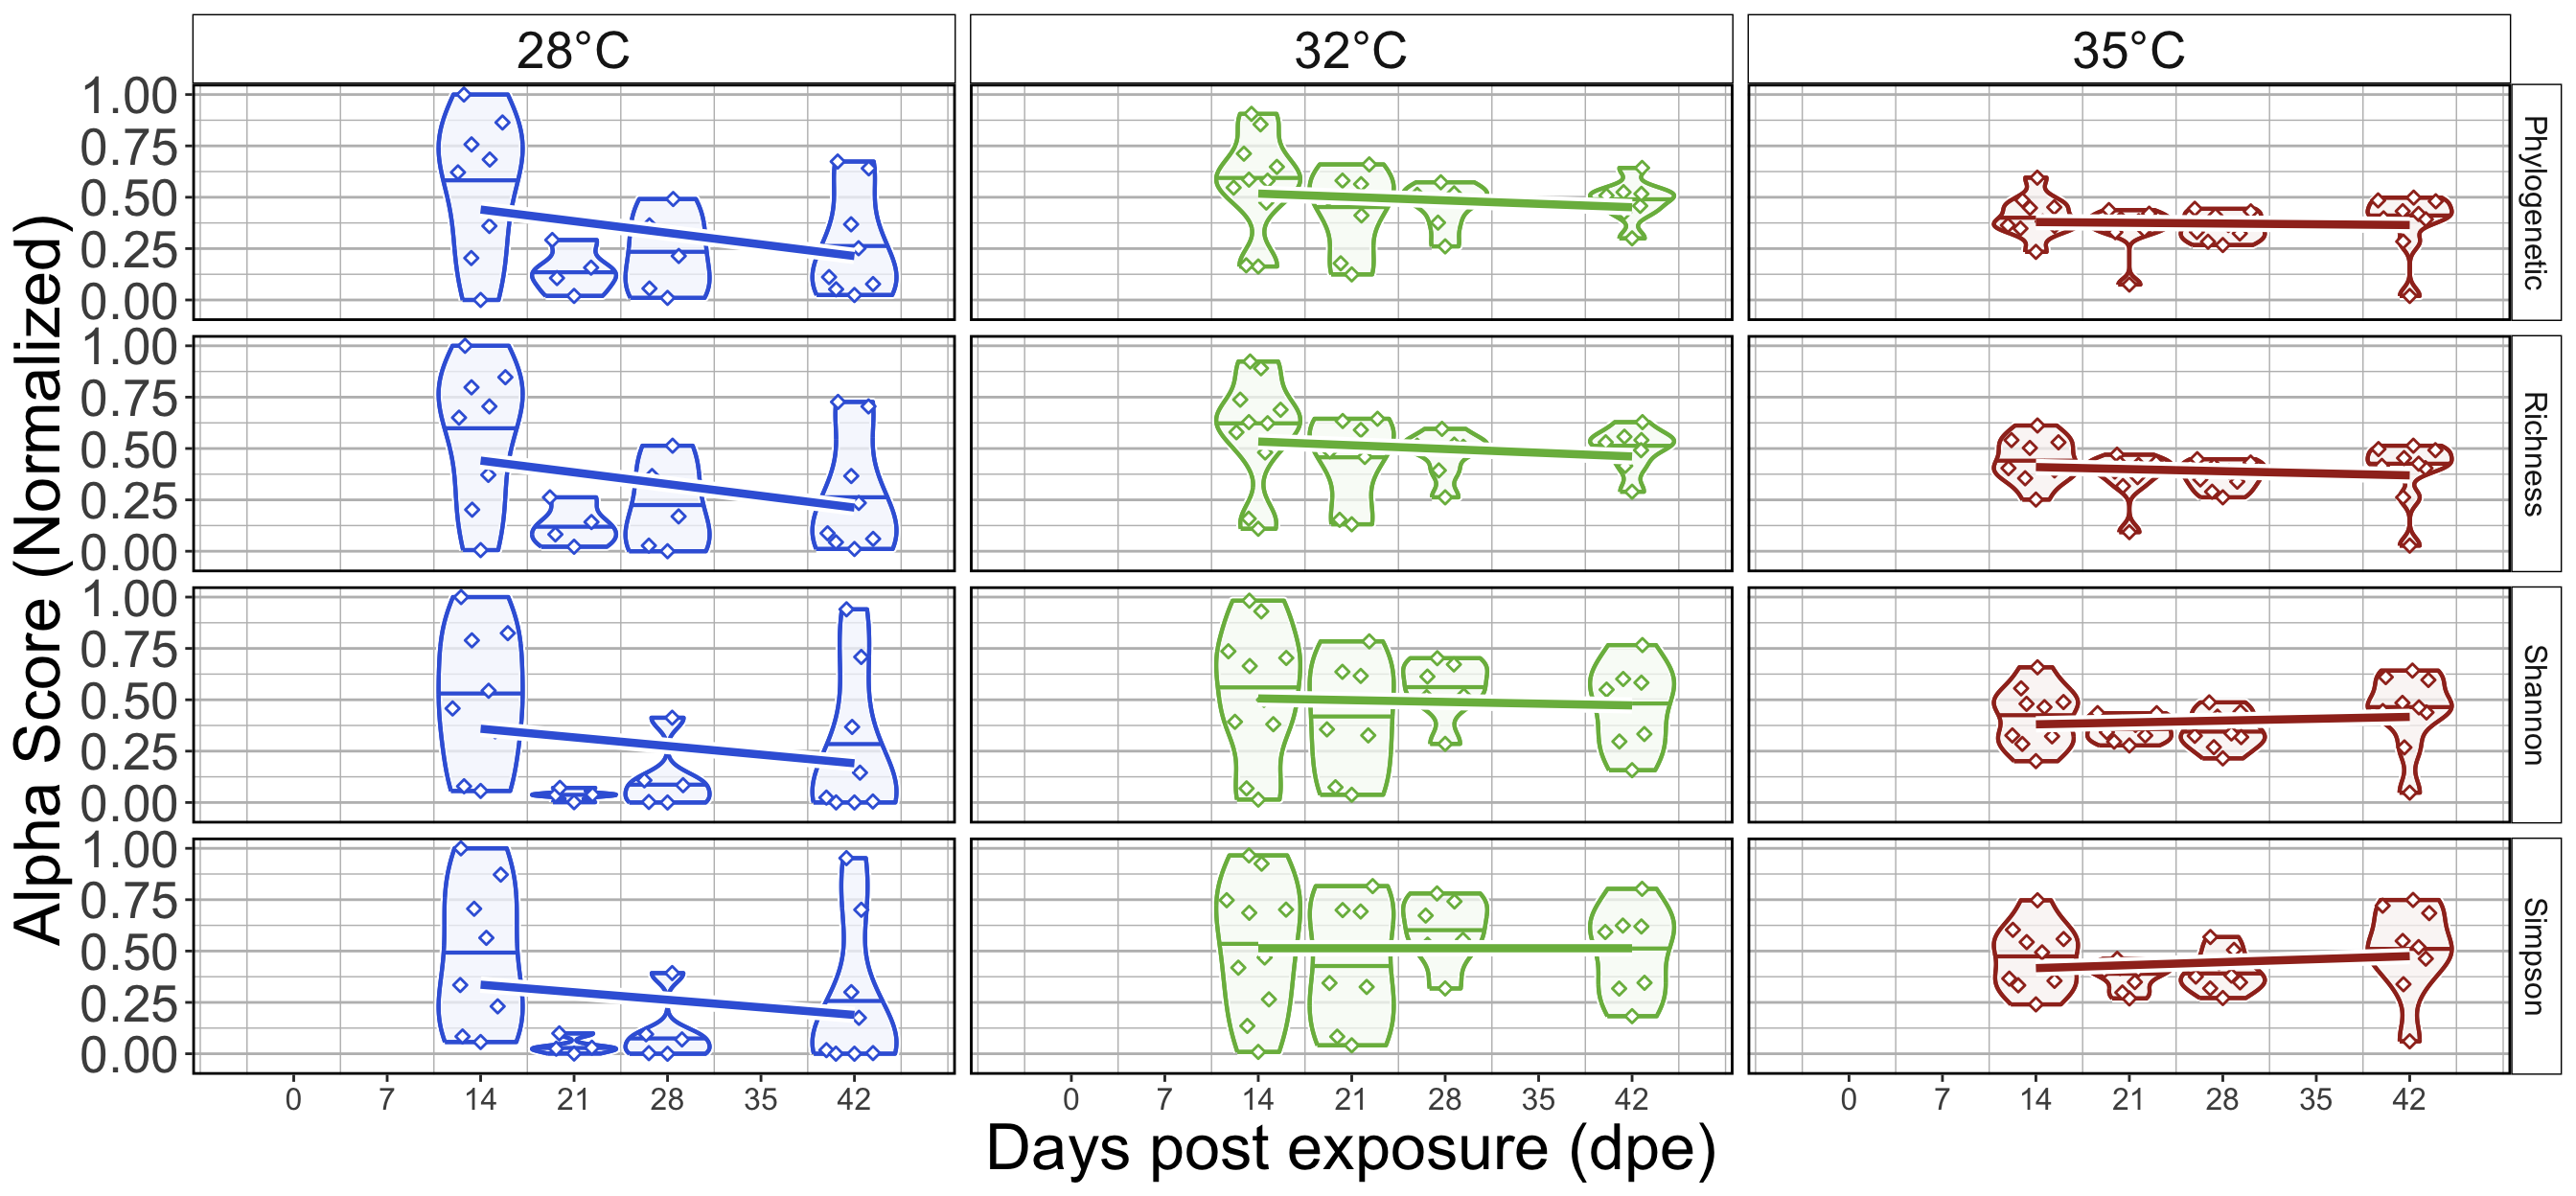
\includegraphics[keepaspectratio]{Results_Overview_files/figure-latex/plots-S4C-1.pdf}}

\paragraph{S4D}\label{s4d}

\pandocbounded{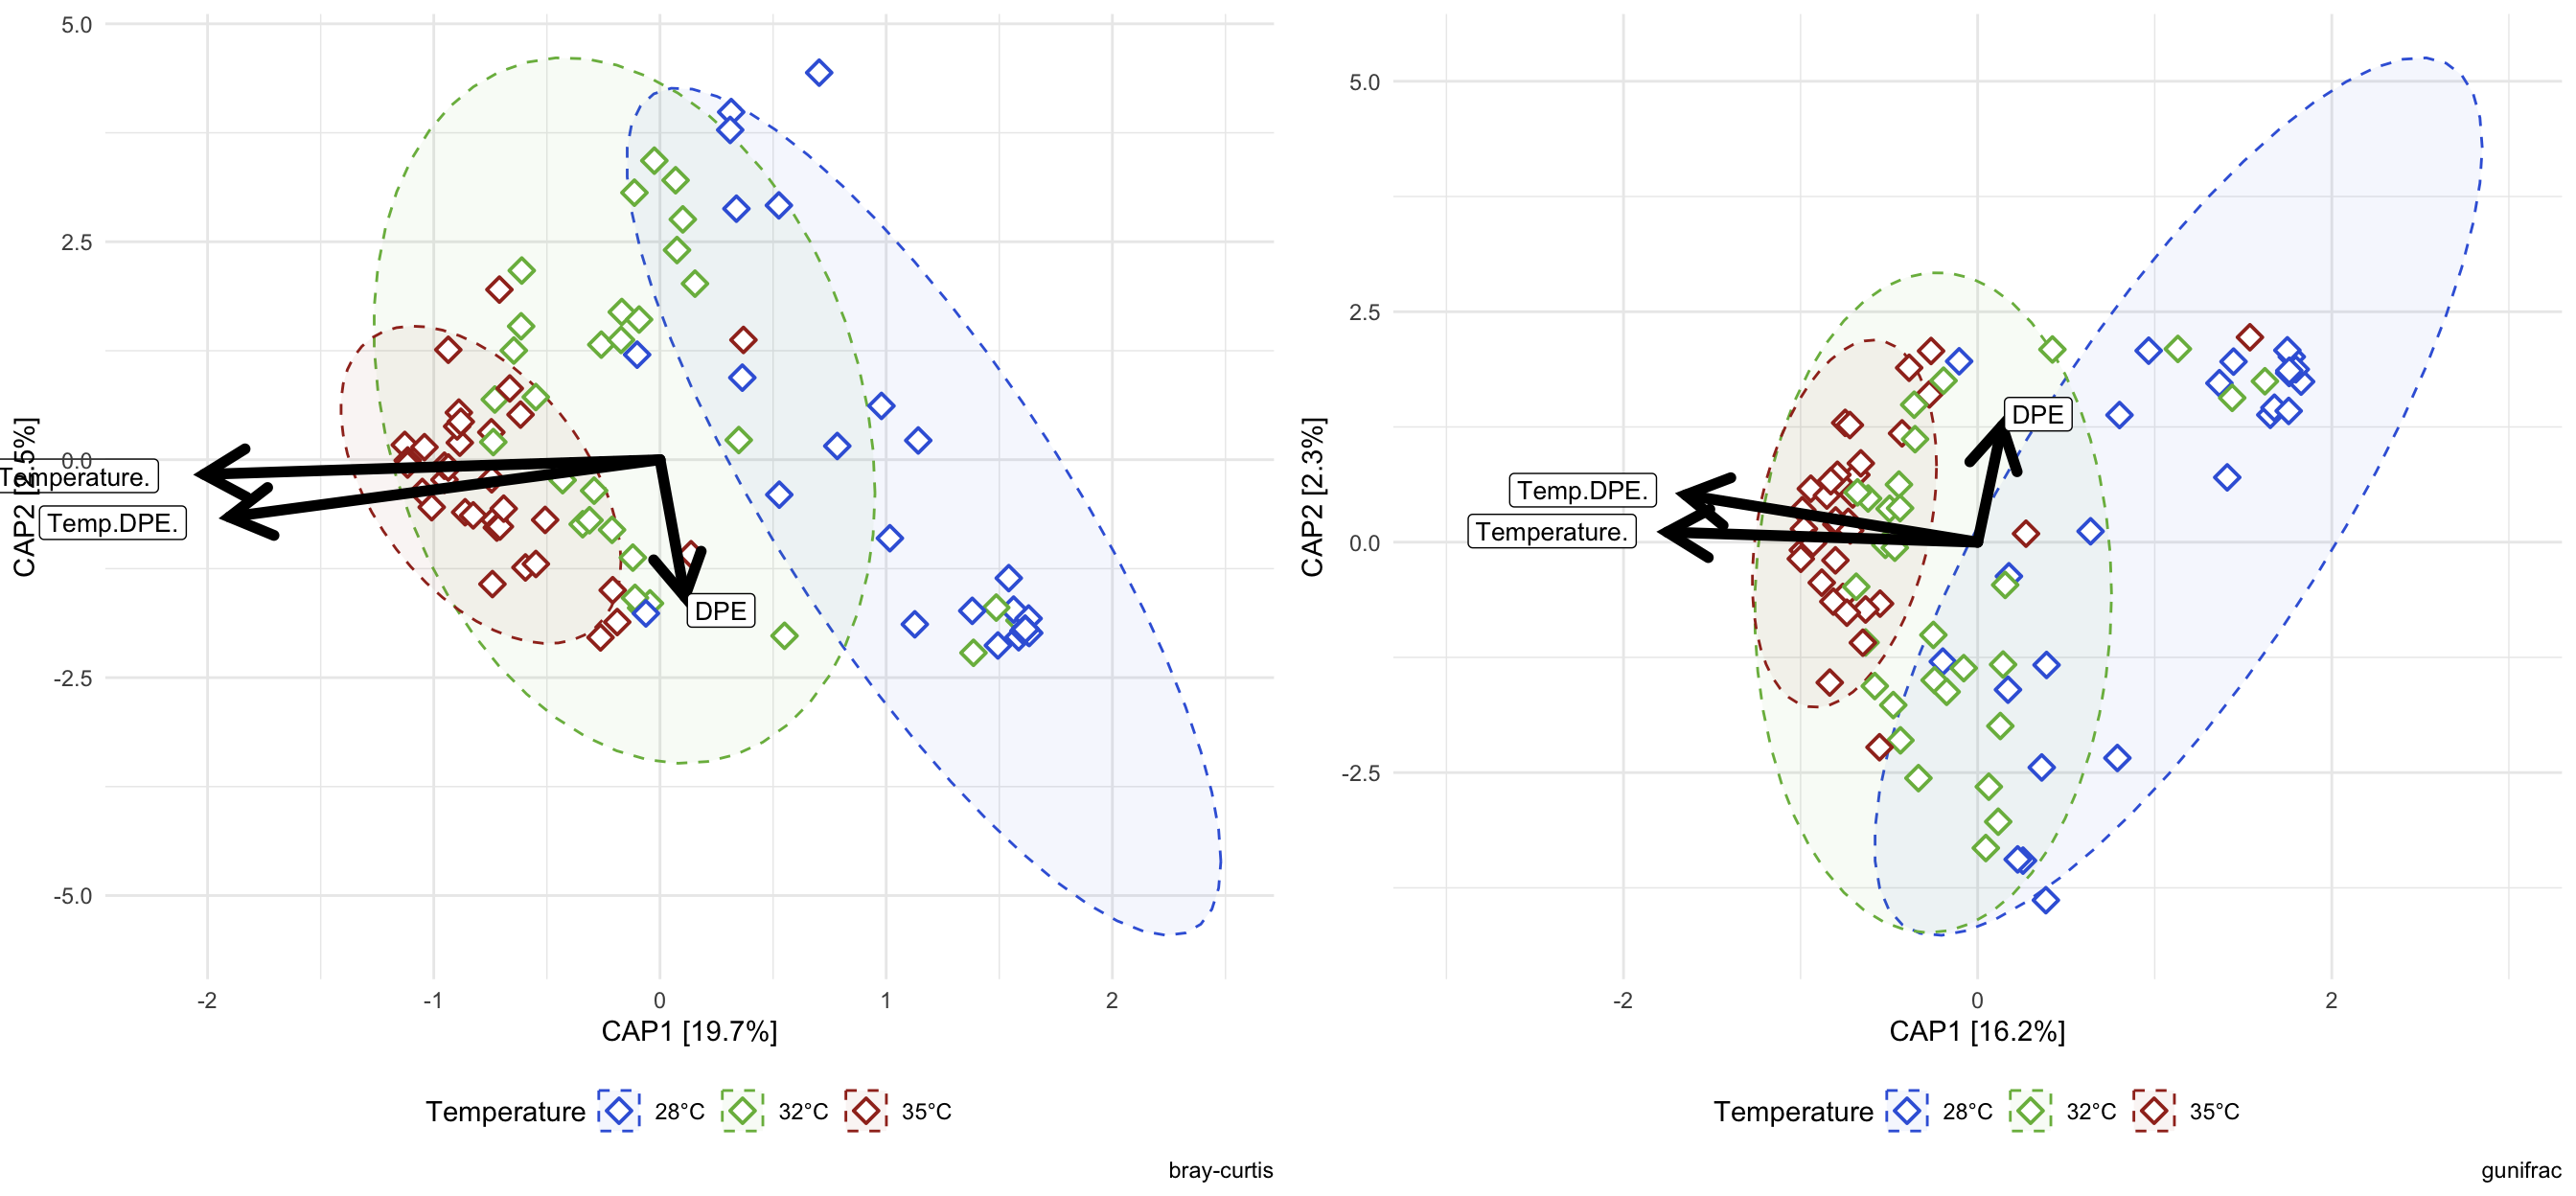
\includegraphics[keepaspectratio]{Results_Overview_files/figure-latex/plots-S4D-1.pdf}}

\subsubsection{Fig. 5) Gut microbiome response has a non-linear
relationship with infection
burden}\label{fig.-5-gut-microbiome-response-has-a-non-linear-relationship-with-infection-burden}

\textbf{Fig. 5} The impacts of presence of infection and infection
burden on the gut microbiomes of Pseudocapillaria tomentosa exposed
zebrafish. (A) Simpson's Index for diversity of parasite exposed fish.
Gut microbial alpha-diversity does not significantly differ between fish
reared at the same water temperature depending on presence of infection.
(B) Capscale ordination based on the Canberra dissimilarity of gut
microbiome composition of parasite exposed fish constrained on the main
effects of temperature and pathology result. The analysis shows that gut
microbiome composition significantly differs between positively infected
fish reared at different water temperatures. (C) Infection burden (total
worm counts ) is positively correlated with lowest or highest alpha
diversity scores in positively infected fish. (D) Capscale ordination
based on the Bray-Curtis dissimilarity of gut microbiome composition
constrained on the main effects of water temperature and infection
burden. The analysis shows that gut microbiome composition significantly
differs between clusters of Low, High and Other fish. Samples points are
colored by water temperature, and filled by cluster grouping. Samples
with at least one detectable worm and an alpha-diversity score less than
0.5 are categorized as Low (orange fill), samples with at least one
detectable worm and an alpha-diversity score greater than 0.5 are
categorized as High (purple fill), and samples with no observable
infection are categorized as Other (white and transparent fill). Ribbons
and ellipses indicate 95\% confidence interval. Only statistically
significant relationships are shown. A ``*'' indicates statistical
significance below the ``0.05'' level. Black arrows indicate
statistically significant covariates and direction of greatest change in
the indicated covariates.

\paragraph{5A)}\label{a-3}

\pandocbounded{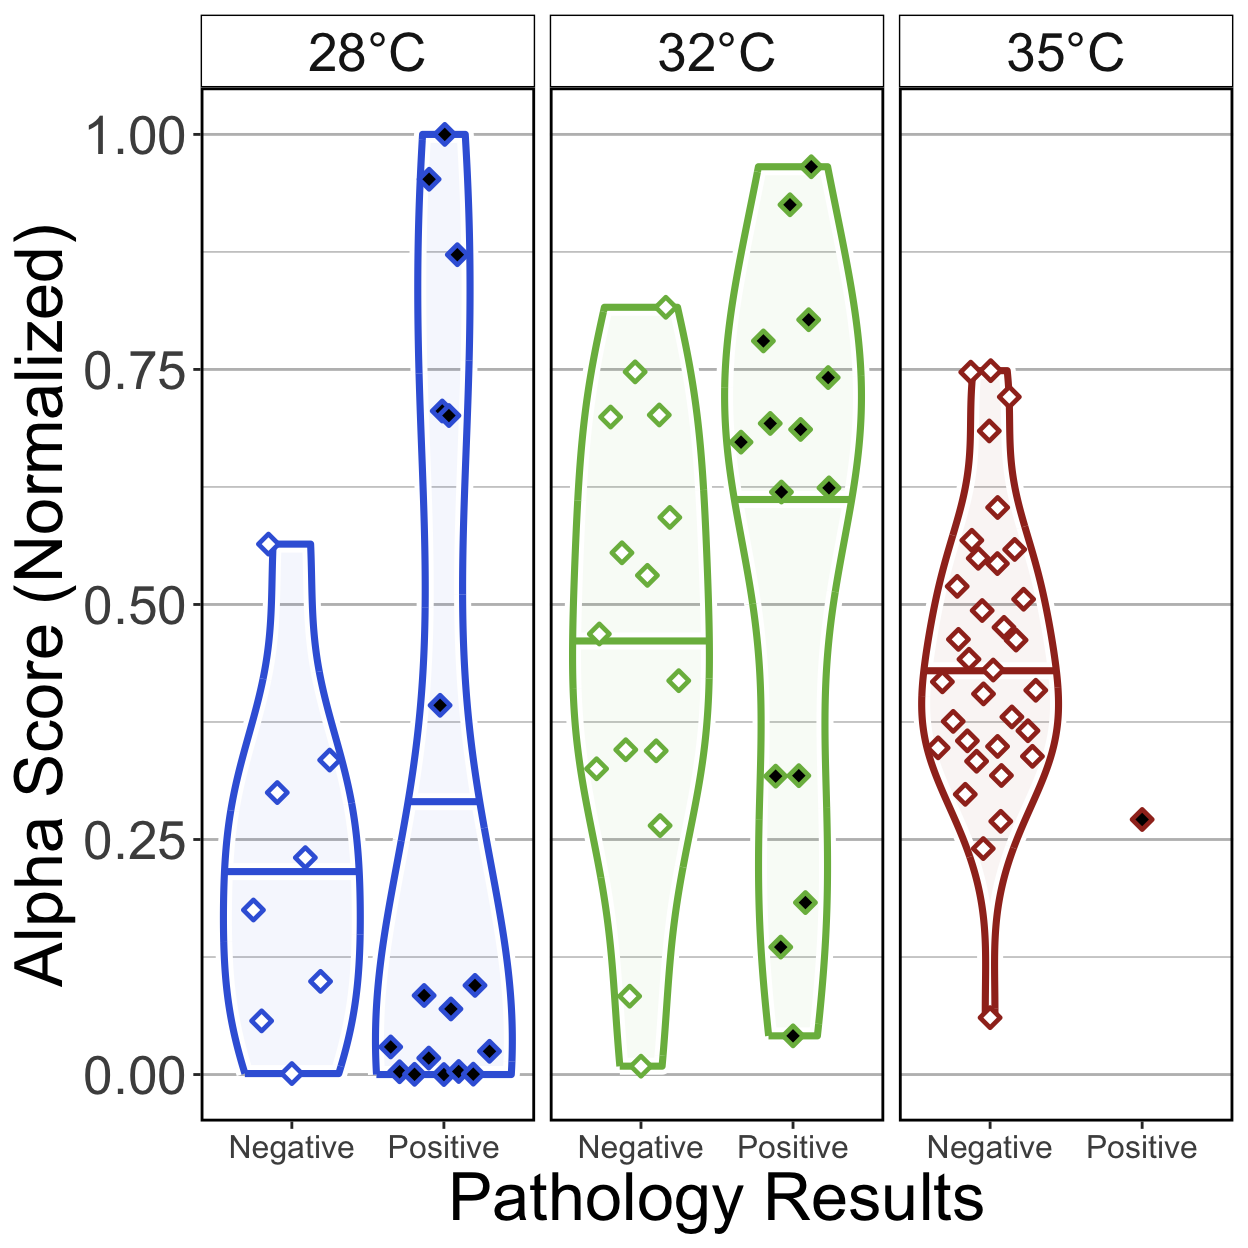
\includegraphics[keepaspectratio]{Results_Overview_files/figure-latex/plots-5A-1.pdf}}

\subparagraph{Tables}\label{tables-11}

(hide)

Click on tabs to display tables. Scroll to see additional rows.

GLM

\begin{longtable}{lrrrrl}
\caption*{
{\large GLM Results} \\ 
{\small glm(Alpha.Score \textasciitilde{} Temperature*Pathology.Results); Exposed fish}
} \\ 
\toprule
term & estimate & std.error & statistic & p.value & p.adj.sig \\ 
\midrule\addlinespace[2.5pt]
\multicolumn{6}{l}{Shannon} \\ 
\midrule\addlinespace[2.5pt]
(Intercept) & $-1.090$ & $0.429$ & $-2.544$ & $0.013$ & * \\ 
Temperature32 & $0.889$ & $0.508$ & $1.749$ & $0.084$ & ns \\ 
Temperature35 & $0.693$ & $0.468$ & $1.482$ & $0.142$ & ns \\ 
Pathology.Resultspositive & $0.223$ & $0.512$ & $0.436$ & $\geq$0.25 & ns \\ 
Temperature32:Pathology.Resultspositive & $0.125$ & $0.641$ & $0.195$ & $\geq$0.25 & ns \\ 
Temperature35:Pathology.Resultspositive & $-1.122$ & $1.392$ & $-0.806$ & $\geq$0.25 & ns \\ 
\midrule\addlinespace[2.5pt]
\multicolumn{6}{l}{Simpson} \\ 
\midrule\addlinespace[2.5pt]
(Intercept) & $-1.265$ & $0.458$ & $-2.760$ & $0.007$ & ** \\ 
Temperature32 & $1.105$ & $0.536$ & $2.061$ & $0.042$ & * \\ 
Temperature35 & $1.055$ & $0.495$ & $2.130$ & $0.036$ & * \\ 
Pathology.Resultspositive & $0.375$ & $0.541$ & $0.694$ & $\geq$0.25 & ns \\ 
Temperature32:Pathology.Resultspositive & $0.054$ & $0.669$ & $0.081$ & $\geq$0.25 & ns \\ 
Temperature35:Pathology.Resultspositive & $-1.154$ & $1.337$ & $-0.863$ & $\geq$0.25 & ns \\ 
\midrule\addlinespace[2.5pt]
\multicolumn{6}{l}{Richness} \\ 
\midrule\addlinespace[2.5pt]
(Intercept) & $-0.421$ & $0.329$ & $-1.279$ & $0.204$ & ns \\ 
Temperature32 & $0.483$ & $0.405$ & $1.194$ & $0.236$ & ns \\ 
Temperature35 & $-0.002$ & $0.367$ & $-0.005$ & $\geq$0.25 & ns \\ 
Pathology.Resultspositive & $-0.390$ & $0.407$ & $-0.957$ & $\geq$0.25 & ns \\ 
Temperature32:Pathology.Resultspositive & $0.310$ & $0.526$ & $0.589$ & $\geq$0.25 & ns \\ 
Temperature35:Pathology.Resultspositive & $-0.221$ & $1.125$ & $-0.197$ & $\geq$0.25 & ns \\ 
\midrule\addlinespace[2.5pt]
\multicolumn{6}{l}{Phylogenetic} \\ 
\midrule\addlinespace[2.5pt]
(Intercept) & $-0.421$ & $0.311$ & $-1.353$ & $0.180$ & ns \\ 
Temperature32 & $0.397$ & $0.383$ & $1.037$ & $\geq$0.25 & ns \\ 
Temperature35 & $-0.085$ & $0.348$ & $-0.244$ & $\geq$0.25 & ns \\ 
Pathology.Resultspositive & $-0.390$ & $0.385$ & $-1.014$ & $\geq$0.25 & ns \\ 
Temperature32:Pathology.Resultspositive & $0.373$ & $0.497$ & $0.750$ & $\geq$0.25 & ns \\ 
Temperature35:Pathology.Resultspositive & $-0.112$ & $1.058$ & $-0.105$ & $\geq$0.25 & ns \\ 
\bottomrule
\end{longtable}

ANOVA

\begin{longtable}{lrrrl}
\caption*{
{\large ANOVA of GLM} \\ 
{\small ANOVA(GLM(Alpha.Score \textasciitilde{} Temperature*Time), type = 2); Exposed fish}
} \\ 
\toprule
term & statistic & df & p.value & sig \\ 
\midrule\addlinespace[2.5pt]
\multicolumn{5}{l}{Shannon} \\ 
\midrule\addlinespace[2.5pt]
Temperature & $9.895$ & $2.000$ & $0.007$ & ** \\ 
Pathology.Results & $0.569$ & $1.000$ & $\geq$0.25 & ns \\ 
Temperature:Pathology.Results & $0.997$ & $2.000$ & $\geq$0.25 & ns \\ 
\midrule\addlinespace[2.5pt]
\multicolumn{5}{l}{Simpson} \\ 
\midrule\addlinespace[2.5pt]
Temperature & $13.663$ & $2.000$ & $0.001$ & ** \\ 
Pathology.Results & $1.134$ & $1.000$ & $\geq$0.25 & ns \\ 
Temperature:Pathology.Results & $0.999$ & $2.000$ & $\geq$0.25 & ns \\ 
\midrule\addlinespace[2.5pt]
\multicolumn{5}{l}{Richness} \\ 
\midrule\addlinespace[2.5pt]
Temperature & $8.625$ & $2.000$ & $0.013$ & * \\ 
Pathology.Results & $0.840$ & $1.000$ & $\geq$0.25 & ns \\ 
Temperature:Pathology.Results & $0.495$ & $2.000$ & $\geq$0.25 & ns \\ 
\midrule\addlinespace[2.5pt]
\multicolumn{5}{l}{Phylogenetic} \\ 
\midrule\addlinespace[2.5pt]
Temperature & $8.874$ & $2.000$ & $0.012$ & * \\ 
Pathology.Results & $0.625$ & $1.000$ & $\geq$0.25 & ns \\ 
Temperature:Pathology.Results & $0.674$ & $2.000$ & $\geq$0.25 & ns \\ 
\bottomrule
\end{longtable}

Tukey

\begin{longtable}{cllllrrrrlc}
\caption*{
{\large Pairwise Tukey's HSD, p.adj: Dunnett} \\ 
{\small Tukey(Alpha.Score \textasciitilde{} Temperature*Time); Exposed fish}
} \\ 
\toprule
Temperature & .y. & term & group1 & group2 & estimate & std.error & statistic & adj.p.value & Variable & Group \\ 
\midrule\addlinespace[2.5pt]
\multicolumn{11}{l}{Shannon} \\ 
\midrule\addlinespace[2.5pt]
28 & Alpha.Score & Pathology.Results & positive & negative & $0.223$ & $0.732$ & $0.305$ & $\geq$0.25 & Pathology.Results & 28 \\ 
32 & Alpha.Score & Pathology.Results & positive & negative & $0.348$ & $0.383$ & $0.908$ & $\geq$0.25 & Pathology.Results & 32 \\ 
35 & Alpha.Score & Pathology.Results & positive & negative & $-0.899$ & $0.659$ & $-1.365$ & $0.172$ & Pathology.Results & 35 \\ 
\midrule\addlinespace[2.5pt]
\multicolumn{11}{l}{Simpson} \\ 
\midrule\addlinespace[2.5pt]
28 & Alpha.Score & Pathology.Results & positive & negative & $0.375$ & $0.754$ & $0.497$ & $\geq$0.25 & Pathology.Results & 28 \\ 
32 & Alpha.Score & Pathology.Results & positive & negative & $0.429$ & $0.394$ & $1.089$ & $\geq$0.25 & Pathology.Results & 32 \\ 
35 & Alpha.Score & Pathology.Results & positive & negative & $-0.779$ & $0.692$ & $-1.125$ & $\geq$0.25 & Pathology.Results & 35 \\ 
\midrule\addlinespace[2.5pt]
\multicolumn{11}{l}{Richness} \\ 
\midrule\addlinespace[2.5pt]
28 & Alpha.Score & Pathology.Results & positive & negative & $-0.390$ & $0.608$ & $-0.641$ & $\geq$0.25 & Pathology.Results & 28 \\ 
32 & Alpha.Score & Pathology.Results & positive & negative & $-0.080$ & $0.301$ & $-0.267$ & $\geq$0.25 & Pathology.Results & 32 \\ 
35 & Alpha.Score & Pathology.Results & positive & negative & $-0.611$ & $0.552$ & $-1.107$ & $\geq$0.25 & Pathology.Results & 35 \\ 
\midrule\addlinespace[2.5pt]
\multicolumn{11}{l}{Phylogenetic} \\ 
\midrule\addlinespace[2.5pt]
28 & Alpha.Score & Pathology.Results & positive & negative & $-0.390$ & $0.577$ & $-0.676$ & $\geq$0.25 & Pathology.Results & 28 \\ 
32 & Alpha.Score & Pathology.Results & positive & negative & $-0.017$ & $0.280$ & $-0.062$ & $\geq$0.25 & Pathology.Results & 32 \\ 
35 & Alpha.Score & Pathology.Results & positive & negative & $-0.502$ & $0.524$ & $-0.958$ & $\geq$0.25 & Pathology.Results & 35 \\ 
\bottomrule
\end{longtable}

\subparagraph{Addl. Metrics}\label{addl.-metrics-8}

\paragraph{5B)}\label{b-3}

\pandocbounded{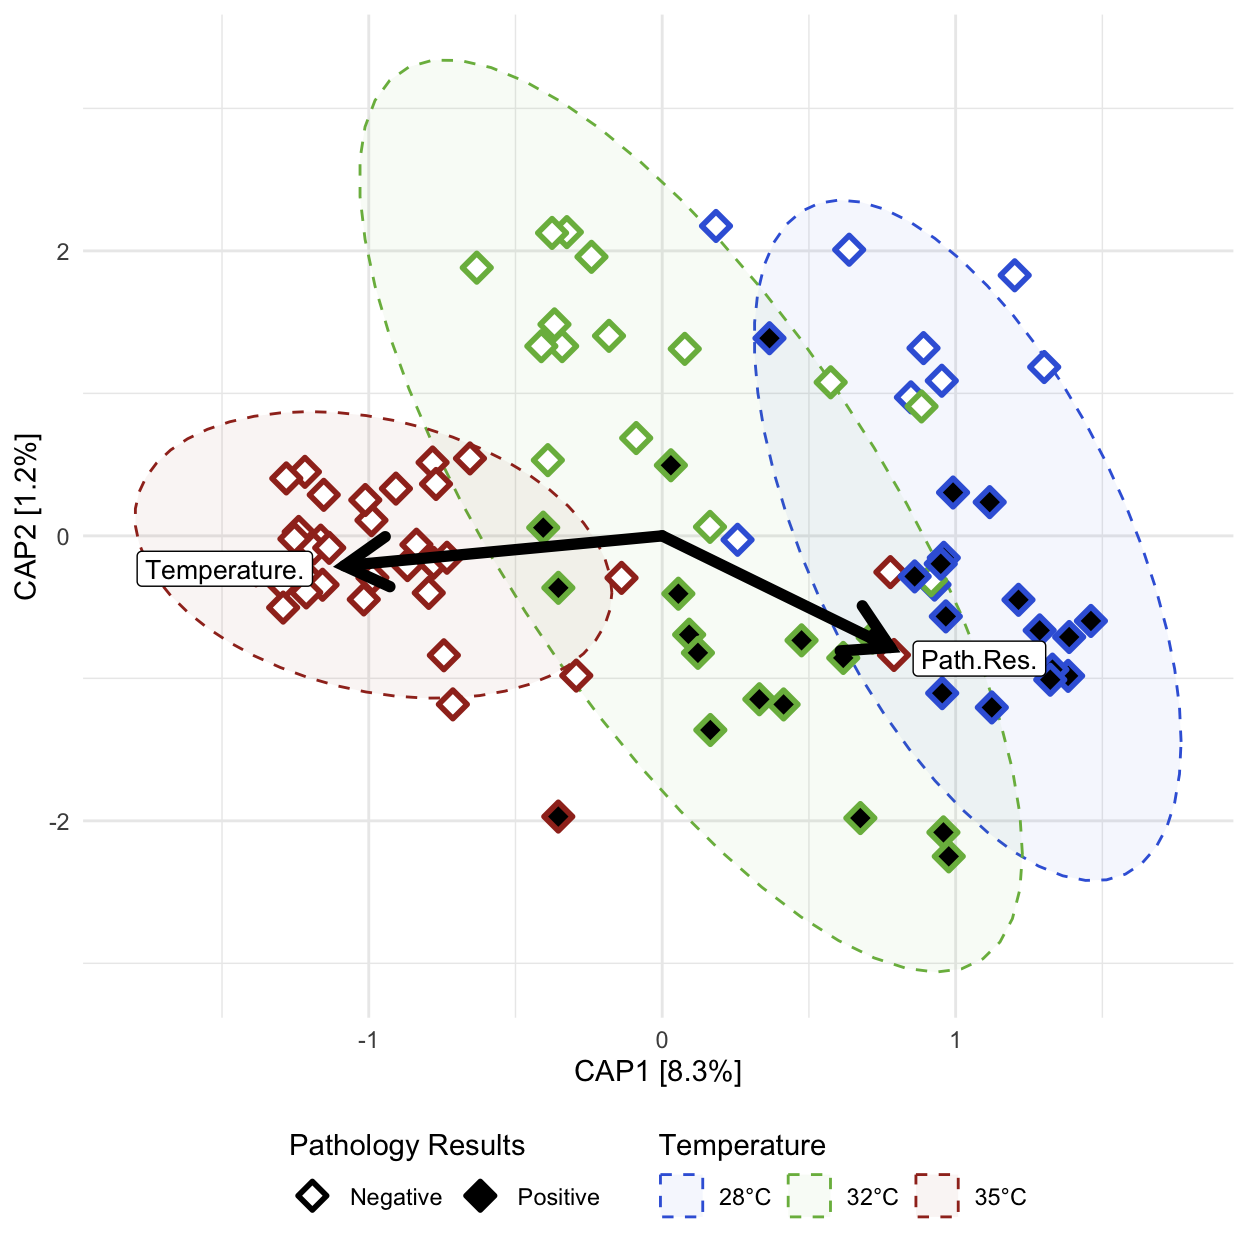
\includegraphics[keepaspectratio]{Results_Overview_files/figure-latex/plots-5B-1.pdf}}

\subparagraph{Tables}\label{tables-12}

(hide)

Click on tabs to display tables. Scroll to see additional rows.

ADONIS2

\begin{longtable}{lrrrrrl}
\caption*{
{\large ADONIS2} \\ 
{\small adonis2(Beta Distance \textasciitilde{} Temperature*Pathology.Results); Exposed fish}
} \\ 
\toprule
term & df & SumOfSqs & R2 & statistic & p.value & sig \\ 
\midrule\addlinespace[2.5pt]
\multicolumn{7}{l}{bray} \\ 
\midrule\addlinespace[2.5pt]
Temperature & $2.000$ & $5.218$ & $0.251$ & $14.569$ & $0.001$ & *** \\ 
Pathology.Results & $1.000$ & $0.263$ & $0.013$ & $1.471$ & $0.179$ & ns \\ 
Temperature:Pathology.Results & $2.000$ & $0.404$ & $0.019$ & $1.127$ & $\geq$0.25 & ns \\ 
Residual & $83.000$ & $14.863$ & $0.716$ & NA & NA & NA \\ 
Total & $88.000$ & $20.748$ & $1.000$ & NA & NA & NA \\ 
\midrule\addlinespace[2.5pt]
\multicolumn{7}{l}{canberra} \\ 
\midrule\addlinespace[2.5pt]
Temperature & $2.000$ & $3.573$ & $0.117$ & $5.751$ & $0.001$ & *** \\ 
Pathology.Results & $1.000$ & $0.488$ & $0.016$ & $1.570$ & $0.029$ & * \\ 
Temperature:Pathology.Results & $2.000$ & $0.679$ & $0.022$ & $1.093$ & $\geq$0.25 & ns \\ 
Residual & $83.000$ & $25.781$ & $0.845$ & NA & NA & NA \\ 
Total & $88.000$ & $30.520$ & $1.000$ & NA & NA & NA \\ 
\midrule\addlinespace[2.5pt]
\multicolumn{7}{l}{gunifrac} \\ 
\midrule\addlinespace[2.5pt]
Temperature & $2.000$ & $3.363$ & $0.212$ & $11.651$ & $0.001$ & *** \\ 
Pathology.Results & $1.000$ & $0.234$ & $0.015$ & $1.622$ & $0.141$ & ns \\ 
Temperature:Pathology.Results & $2.000$ & $0.264$ & $0.017$ & $0.915$ & $\geq$0.25 & ns \\ 
Residual & $83.000$ & $11.980$ & $0.756$ & NA & NA & NA \\ 
Total & $88.000$ & $15.841$ & $1.000$ & NA & NA & NA \\ 
\bottomrule
\end{longtable}

Dispersion (ANOVA)

\begin{longtable}{lrrrrrr}
\caption*{
{\large ANOVA: Homogeneity of Dispersion} \\ 
{\small ANOVA(Beta Disperson \textasciitilde{} Temperature*Pathology.Results); Exposed fish}
} \\ 
\toprule
term & df & sumsq & meansq & statistic & p.value & sig \\ 
\midrule\addlinespace[2.5pt]
\multicolumn{7}{l}{bray} \\ 
\midrule\addlinespace[2.5pt]
Temp.Path & $5.000$ & $0.520$ & $0.104$ & $4.652$ & <0.001 & *** \\ 
Residual & $83.000$ & $1.855$ & $0.022$ & NA & NA & NA \\ 
\midrule\addlinespace[2.5pt]
\multicolumn{7}{l}{canberra} \\ 
\midrule\addlinespace[2.5pt]
Temp.Path & $5.000$ & $0.625$ & $0.125$ & $13.830$ & <0.001 & **** \\ 
Residual & $83.000$ & $0.750$ & $0.009$ & NA & NA & NA \\ 
\midrule\addlinespace[2.5pt]
\multicolumn{7}{l}{gunifrac} \\ 
\midrule\addlinespace[2.5pt]
Temp.Path & $5.000$ & $0.436$ & $0.087$ & $6.954$ & <0.001 & **** \\ 
Residual & $83.000$ & $1.040$ & $0.013$ & NA & NA & NA \\ 
\bottomrule
\end{longtable}

Dispersion (Tukey)

\begin{longtable}{llllrrrrl}
\caption*{
{\large Tukey: Homogeneity of Dispersion} \\ 
{\small Tukey(Beta Disperson \textasciitilde{} Temperature*Pathology.Results); Exposed fish}
} \\ 
\toprule
.y. & term & group1 & group2 & estimate & conf.low & conf.high & adj.p.value & sig \\ 
\midrule\addlinespace[2.5pt]
\multicolumn{9}{l}{bray} \\ 
\midrule\addlinespace[2.5pt]
Distance & Temp.Path & 28°C\_\_pos & 28°C\_\_neg & $0.022$ & $-0.165$ & $0.209$ & $\geq$0.25 & ns \\ 
Distance & Temp.Path & 32°C\_\_neg & 28°C\_\_neg & $-0.086$ & $-0.277$ & $0.105$ & $\geq$0.25 & ns \\ 
Distance & Temp.Path & 32°C\_\_pos & 28°C\_\_neg & $0.015$ & $-0.176$ & $0.206$ & $\geq$0.25 & ns \\ 
Distance & Temp.Path & 35°C\_\_neg & 28°C\_\_neg & $-0.126$ & $-0.298$ & $0.046$ & $\geq$0.25 & ns \\ 
Distance & Temp.Path & 35°C\_\_pos & 28°C\_\_neg & $-0.434$ & $-0.896$ & $0.029$ & $0.079$ & ns \\ 
Distance & Temp.Path & 32°C\_\_neg & 28°C\_\_pos & $-0.108$ & $-0.263$ & $0.046$ & $\geq$0.25 & ns \\ 
Distance & Temp.Path & 32°C\_\_pos & 28°C\_\_pos & $-0.007$ & $-0.161$ & $0.148$ & $\geq$0.25 & ns \\ 
Distance & Temp.Path & 35°C\_\_neg & 28°C\_\_pos & $-0.148$ & $-0.278$ & $-0.017$ & $0.017$ & * \\ 
Distance & Temp.Path & 35°C\_\_pos & 28°C\_\_pos & $-0.456$ & $-0.905$ & $-0.007$ & $0.044$ & * \\ 
Distance & Temp.Path & 32°C\_\_pos & 32°C\_\_neg & $0.101$ & $-0.058$ & $0.261$ & $\geq$0.25 & ns \\ 
Distance & Temp.Path & 35°C\_\_neg & 32°C\_\_neg & $-0.039$ & $-0.175$ & $0.096$ & $\geq$0.25 & ns \\ 
Distance & Temp.Path & 35°C\_\_pos & 32°C\_\_neg & $-0.348$ & $-0.798$ & $0.103$ & $0.226$ & ns \\ 
Distance & Temp.Path & 35°C\_\_neg & 32°C\_\_pos & $-0.141$ & $-0.277$ & $-0.005$ & $0.038$ & * \\ 
Distance & Temp.Path & 35°C\_\_pos & 32°C\_\_pos & $-0.449$ & $-0.899$ & $0.001$ & $0.051$ & ns \\ 
Distance & Temp.Path & 35°C\_\_pos & 35°C\_\_neg & $-0.308$ & $-0.751$ & $0.135$ & $\geq$0.25 & ns \\ 
\midrule\addlinespace[2.5pt]
\multicolumn{9}{l}{canberra} \\ 
\midrule\addlinespace[2.5pt]
Distance & Temp.Path & 28°C\_\_pos & 28°C\_\_neg & $0.045$ & $-0.074$ & $0.164$ & $\geq$0.25 & ns \\ 
Distance & Temp.Path & 32°C\_\_neg & 28°C\_\_neg & $-0.123$ & $-0.244$ & $-0.002$ & $0.045$ & * \\ 
Distance & Temp.Path & 32°C\_\_pos & 28°C\_\_neg & $-0.042$ & $-0.164$ & $0.079$ & $\geq$0.25 & ns \\ 
Distance & Temp.Path & 35°C\_\_neg & 28°C\_\_neg & $-0.105$ & $-0.214$ & $0.005$ & $0.068$ & ns \\ 
Distance & Temp.Path & 35°C\_\_pos & 28°C\_\_neg & $-0.588$ & $-0.883$ & $-0.294$ & <0.001 & **** \\ 
Distance & Temp.Path & 32°C\_\_neg & 28°C\_\_pos & $-0.168$ & $-0.267$ & $-0.070$ & <0.001 & **** \\ 
Distance & Temp.Path & 32°C\_\_pos & 28°C\_\_pos & $-0.088$ & $-0.186$ & $0.010$ & $0.107$ & ns \\ 
Distance & Temp.Path & 35°C\_\_neg & 28°C\_\_pos & $-0.150$ & $-0.233$ & $-0.067$ & <0.001 & **** \\ 
Distance & Temp.Path & 35°C\_\_pos & 28°C\_\_pos & $-0.634$ & $-0.919$ & $-0.348$ & <0.001 & **** \\ 
Distance & Temp.Path & 32°C\_\_pos & 32°C\_\_neg & $0.080$ & $-0.021$ & $0.182$ & $0.199$ & ns \\ 
Distance & Temp.Path & 35°C\_\_neg & 32°C\_\_neg & $0.018$ & $-0.068$ & $0.105$ & $\geq$0.25 & ns \\ 
Distance & Temp.Path & 35°C\_\_pos & 32°C\_\_neg & $-0.465$ & $-0.752$ & $-0.179$ & <0.001 & *** \\ 
Distance & Temp.Path & 35°C\_\_neg & 32°C\_\_pos & $-0.062$ & $-0.149$ & $0.024$ & $\geq$0.25 & ns \\ 
Distance & Temp.Path & 35°C\_\_pos & 32°C\_\_pos & $-0.546$ & $-0.832$ & $-0.259$ & <0.001 & **** \\ 
Distance & Temp.Path & 35°C\_\_pos & 35°C\_\_neg & $-0.484$ & $-0.765$ & $-0.202$ & <0.001 & **** \\ 
\midrule\addlinespace[2.5pt]
\multicolumn{9}{l}{gunifrac} \\ 
\midrule\addlinespace[2.5pt]
Distance & Temp.Path & 28°C\_\_pos & 28°C\_\_neg & $0.011$ & $-0.129$ & $0.151$ & $\geq$0.25 & ns \\ 
Distance & Temp.Path & 32°C\_\_neg & 28°C\_\_neg & $-0.091$ & $-0.234$ & $0.052$ & $\geq$0.25 & ns \\ 
Distance & Temp.Path & 32°C\_\_pos & 28°C\_\_neg & $-0.014$ & $-0.157$ & $0.129$ & $\geq$0.25 & ns \\ 
Distance & Temp.Path & 35°C\_\_neg & 28°C\_\_neg & $-0.129$ & $-0.258$ & $0.000$ & $0.049$ & * \\ 
Distance & Temp.Path & 35°C\_\_pos & 28°C\_\_neg & $-0.411$ & $-0.758$ & $-0.065$ & $0.011$ & * \\ 
Distance & Temp.Path & 32°C\_\_neg & 28°C\_\_pos & $-0.102$ & $-0.218$ & $0.014$ & $0.115$ & ns \\ 
Distance & Temp.Path & 32°C\_\_pos & 28°C\_\_pos & $-0.025$ & $-0.141$ & $0.091$ & $\geq$0.25 & ns \\ 
Distance & Temp.Path & 35°C\_\_neg & 28°C\_\_pos & $-0.140$ & $-0.238$ & $-0.043$ & <0.001 & *** \\ 
Distance & Temp.Path & 35°C\_\_pos & 28°C\_\_pos & $-0.423$ & $-0.759$ & $-0.087$ & $0.006$ & ** \\ 
Distance & Temp.Path & 32°C\_\_pos & 32°C\_\_neg & $0.077$ & $-0.042$ & $0.196$ & $\geq$0.25 & ns \\ 
Distance & Temp.Path & 35°C\_\_neg & 32°C\_\_neg & $-0.038$ & $-0.140$ & $0.064$ & $\geq$0.25 & ns \\ 
Distance & Temp.Path & 35°C\_\_pos & 32°C\_\_neg & $-0.321$ & $-0.658$ & $0.017$ & $0.072$ & ns \\ 
Distance & Temp.Path & 35°C\_\_neg & 32°C\_\_pos & $-0.115$ & $-0.217$ & $-0.013$ & $0.017$ & * \\ 
Distance & Temp.Path & 35°C\_\_pos & 32°C\_\_pos & $-0.398$ & $-0.735$ & $-0.060$ & $0.011$ & * \\ 
Distance & Temp.Path & 35°C\_\_pos & 35°C\_\_neg & $-0.283$ & $-0.614$ & $0.049$ & $0.140$ & ns \\ 
\bottomrule
\end{longtable}

\subparagraph{Addl. Metrics}\label{addl.-metrics-9}

\paragraph{5C)}\label{c-2}

\pandocbounded{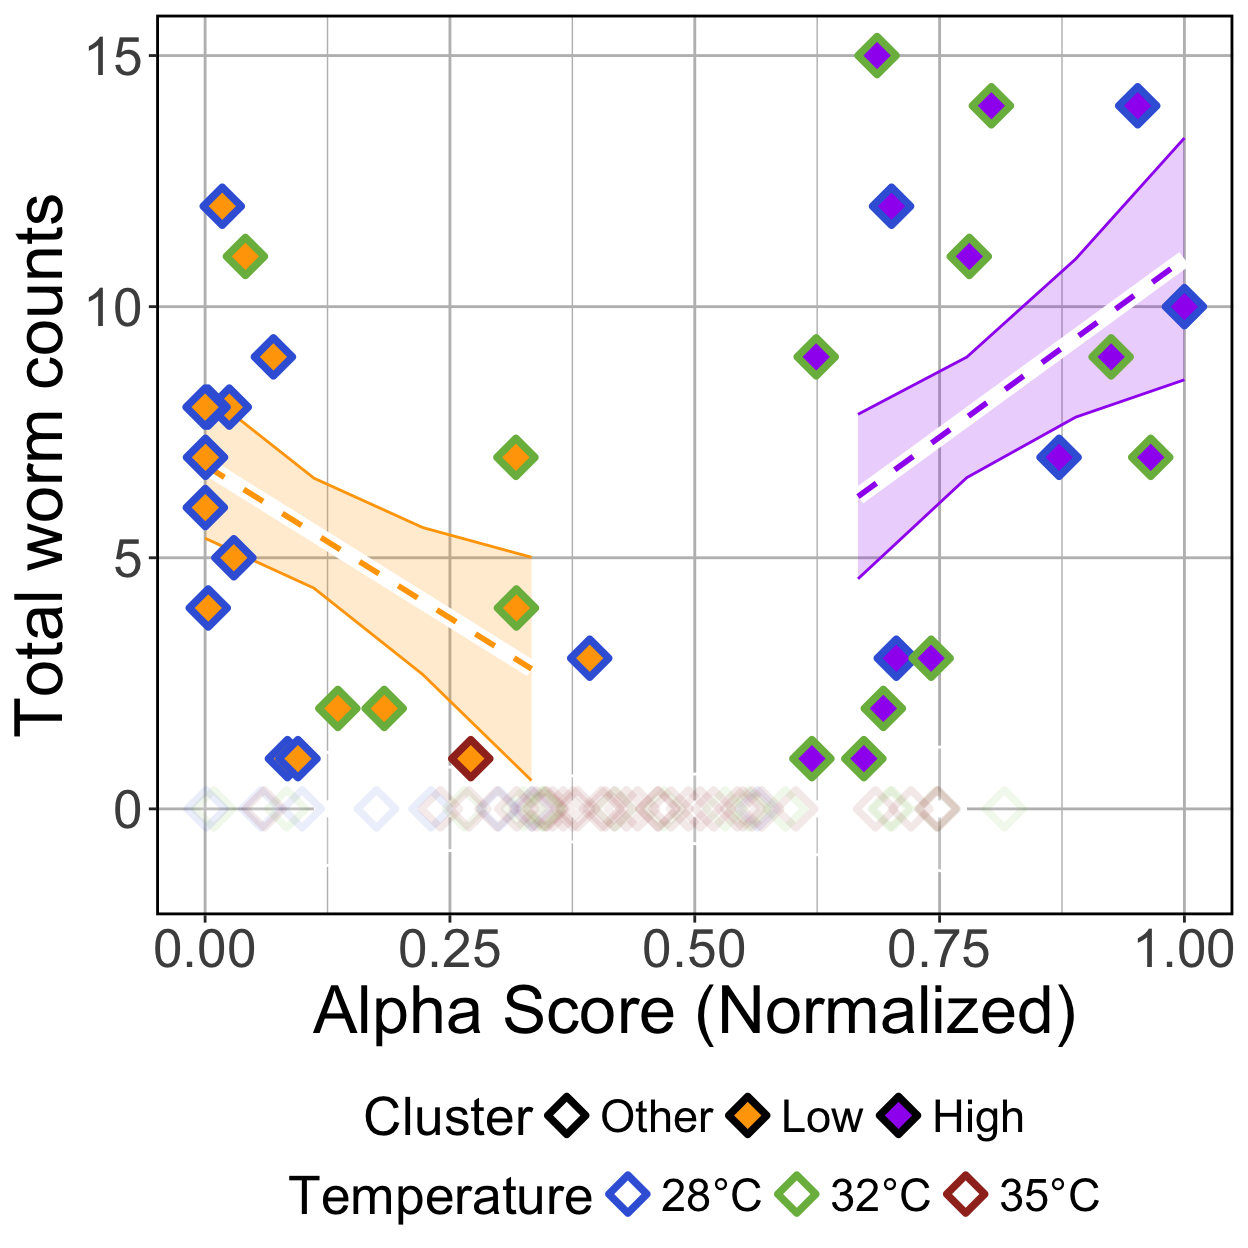
\includegraphics[keepaspectratio]{Results_Overview_files/figure-latex/plots-5C-1.pdf}}

\subparagraph{Tables}\label{tables-13}

(hide)

Click on tabs to display tables. Scroll to see additional rows.

GLM

\begin{longtable}{lrrrrl}
\caption*{
{\large GLM Results} \\ 
{\small glm(Total.Worm.Count \textasciitilde{} Alpha.Score*Cluster); Exposed fish}
} \\ 
\toprule
term & estimate & std.error & statistic & p.value & p.adj.sig \\ 
\midrule\addlinespace[2.5pt]
\multicolumn{6}{l}{Shannon} \\ 
\midrule\addlinespace[2.5pt]
(Intercept) & $0.000$ & $0.778$ & $0.000$ & $\geq$0.25 & ns \\ 
Alpha.Score & $0.000$ & $1.808$ & $0.000$ & $\geq$0.25 & ns \\ 
ClusterLow & $6.524$ & $1.067$ & $6.115$ & <0.001 & **** \\ 
ClusterHigh & $-2.610$ & $3.512$ & $-0.743$ & $\geq$0.25 & ns \\ 
Alpha.Score:ClusterLow & $-10.090$ & $4.999$ & $-2.018$ & $0.047$ & * \\ 
Alpha.Score:ClusterHigh & $13.706$ & $4.766$ & $2.876$ & $0.005$ & ** \\ 
\midrule\addlinespace[2.5pt]
\multicolumn{6}{l}{Simpson} \\ 
\midrule\addlinespace[2.5pt]
(Intercept) & $0.000$ & $0.741$ & $0.000$ & $\geq$0.25 & ns \\ 
Alpha.Score & $0.000$ & $1.605$ & $0.000$ & $\geq$0.25 & ns \\ 
ClusterLow & $6.842$ & $1.041$ & $6.573$ & <0.001 & **** \\ 
ClusterHigh & $-3.247$ & $3.900$ & $-0.833$ & $\geq$0.25 & ns \\ 
Alpha.Score:ClusterLow & $-12.165$ & $4.647$ & $-2.618$ & $0.011$ & * \\ 
Alpha.Score:ClusterHigh & $14.198$ & $5.090$ & $2.789$ & $0.007$ & ** \\ 
\midrule\addlinespace[2.5pt]
\multicolumn{6}{l}{Richness} \\ 
\midrule\addlinespace[2.5pt]
(Intercept) & $0.000$ & $0.914$ & $0.000$ & $\geq$0.25 & ns \\ 
Alpha.Score & $0.000$ & $1.983$ & $0.000$ & $\geq$0.25 & ns \\ 
ClusterLow & $6.105$ & $1.294$ & $4.717$ & <0.001 & **** \\ 
ClusterHigh & $7.362$ & $2.644$ & $2.784$ & $0.007$ & ** \\ 
Alpha.Score:ClusterLow & $-3.491$ & $4.463$ & $-0.782$ & $\geq$0.25 & ns \\ 
Alpha.Score:ClusterHigh & $0.772$ & $4.163$ & $0.185$ & $\geq$0.25 & ns \\ 
\midrule\addlinespace[2.5pt]
\multicolumn{6}{l}{Phylogenetic} \\ 
\midrule\addlinespace[2.5pt]
(Intercept) & $0.000$ & $0.912$ & $0.000$ & $\geq$0.25 & ns \\ 
Alpha.Score & $0.000$ & $2.061$ & $0.000$ & $\geq$0.25 & ns \\ 
ClusterLow & $6.230$ & $1.346$ & $4.629$ & <0.001 & **** \\ 
ClusterHigh & $8.137$ & $2.589$ & $3.143$ & $0.002$ & ** \\ 
Alpha.Score:ClusterLow & $-3.872$ & $4.662$ & $-0.831$ & $\geq$0.25 & ns \\ 
Alpha.Score:ClusterHigh & $-0.429$ & $4.237$ & $-0.101$ & $\geq$0.25 & ns \\ 
\bottomrule
\end{longtable}

ANOVA

\begin{longtable}{lrrrl}
\caption*{
{\large ANOVA of GLM} \\ 
{\small ANOVA(GLM(Total.Worm.Count \textasciitilde{} Alpha.Score*Cluster), type = 2); Exposed fish}
} \\ 
\toprule
term & statistic & df & p.value & sig \\ 
\midrule\addlinespace[2.5pt]
\multicolumn{5}{l}{Shannon} \\ 
\midrule\addlinespace[2.5pt]
Alpha.Score & $0.143$ & $1.000$ & $\geq$0.25 & ns \\ 
Cluster & $162.212$ & $2.000$ & <0.001 & **** \\ 
Alpha.Score:Cluster & $14.204$ & $2.000$ & <0.001 & *** \\ 
\midrule\addlinespace[2.5pt]
\multicolumn{5}{l}{Simpson} \\ 
\midrule\addlinespace[2.5pt]
Alpha.Score & $0.002$ & $1.000$ & $\geq$0.25 & ns \\ 
Cluster & $168.513$ & $2.000$ & <0.001 & **** \\ 
Alpha.Score:Cluster & $16.419$ & $2.000$ & <0.001 & *** \\ 
\midrule\addlinespace[2.5pt]
\multicolumn{5}{l}{Richness} \\ 
\midrule\addlinespace[2.5pt]
Alpha.Score & $0.066$ & $1.000$ & $\geq$0.25 & ns \\ 
Cluster & $145.539$ & $2.000$ & <0.001 & **** \\ 
Alpha.Score:Cluster & $0.741$ & $2.000$ & $\geq$0.25 & ns \\ 
\midrule\addlinespace[2.5pt]
\multicolumn{5}{l}{Phylogenetic} \\ 
\midrule\addlinespace[2.5pt]
Alpha.Score & $0.175$ & $1.000$ & $\geq$0.25 & ns \\ 
Cluster & $145.520$ & $2.000$ & <0.001 & **** \\ 
Alpha.Score:Cluster & $0.696$ & $2.000$ & $\geq$0.25 & ns \\ 
\bottomrule
\end{longtable}

Tukey

\begin{longtable}{cllllrrrrlc}
\caption*{
{\large Pairwise Tukey's HSD, p.adj: Dunnett} \\ 
{\small Tukey(Total.Worm.Count \textasciitilde{} Alpha.Score*Cluster); Exposed fish}
} \\ 
\toprule
Temperature & .y. & term & group1 & group2 & estimate & std.error & statistic & adj.p.value & Variable & Group \\ 
\midrule\addlinespace[2.5pt]
\multicolumn{11}{l}{Shannon} \\ 
\midrule\addlinespace[2.5pt]
28 & Alpha.Score & Cluster & Low & Other & $-1.594$ & $0.642$ & $-2.483$ & $0.035$ & Cluster & 28 \\ 
28 & Alpha.Score & Cluster & High & Other & $2.844$ & $0.672$ & $4.233$ & <0.001 & Cluster & 28 \\ 
28 & Alpha.Score & Cluster & High & Low & $4.438$ & $0.773$ & $5.741$ & <0.001 & Cluster & 28 \\ 
32 & Alpha.Score & Cluster & Low & Other & $-1.391$ & $0.495$ & $-2.808$ & $0.013$ & Cluster & 32 \\ 
32 & Alpha.Score & Cluster & High & Other & $1.147$ & $0.333$ & $3.443$ & $0.002$ & Cluster & 32 \\ 
32 & Alpha.Score & Cluster & High & Low & $2.538$ & $0.528$ & $4.811$ & <0.001 & Cluster & 32 \\ 
35 & Alpha.Score & Cluster & Low & Other & $-0.899$ & $0.659$ & $-1.365$ & $0.172$ & Cluster & 35 \\ 
\midrule\addlinespace[2.5pt]
\multicolumn{11}{l}{Simpson} \\ 
\midrule\addlinespace[2.5pt]
28 & Alpha.Score & Cluster & Low & Other & $-1.487$ & $0.656$ & $-2.266$ & $0.060$ & Cluster & 28 \\ 
28 & Alpha.Score & Cluster & High & Other & $2.970$ & $0.665$ & $4.466$ & <0.001 & Cluster & 28 \\ 
28 & Alpha.Score & Cluster & High & Low & $4.457$ & $0.767$ & $5.810$ & <0.001 & Cluster & 28 \\ 
32 & Alpha.Score & Cluster & Low & Other & $-1.233$ & $0.487$ & $-2.531$ & $0.030$ & Cluster & 32 \\ 
32 & Alpha.Score & Cluster & High & Other & $1.264$ & $0.354$ & $3.573$ & <0.001 & Cluster & 32 \\ 
32 & Alpha.Score & Cluster & High & Low & $2.497$ & $0.528$ & $4.729$ & <0.001 & Cluster & 32 \\ 
35 & Alpha.Score & Cluster & Low & Other & $-0.779$ & $0.692$ & $-1.125$ & $\geq$0.25 & Cluster & 35 \\ 
\midrule\addlinespace[2.5pt]
\multicolumn{11}{l}{Richness} \\ 
\midrule\addlinespace[2.5pt]
28 & Alpha.Score & Cluster & Low & Other & $-1.430$ & $0.589$ & $-2.429$ & $0.040$ & Cluster & 28 \\ 
28 & Alpha.Score & Cluster & High & Other & $1.367$ & $0.653$ & $2.095$ & $0.090$ & Cluster & 28 \\ 
28 & Alpha.Score & Cluster & High & Low & $2.797$ & $0.692$ & $4.043$ & <0.001 & Cluster & 28 \\ 
32 & Alpha.Score & Cluster & Low & Other & $-1.183$ & $0.387$ & $-3.052$ & $0.006$ & Cluster & 32 \\ 
32 & Alpha.Score & Cluster & High & Other & $0.429$ & $0.278$ & $1.543$ & $\geq$0.25 & Cluster & 32 \\ 
32 & Alpha.Score & Cluster & High & Low & $1.611$ & $0.410$ & $3.934$ & <0.001 & Cluster & 32 \\ 
35 & Alpha.Score & Cluster & Low & Other & $-0.611$ & $0.552$ & $-1.107$ & $\geq$0.25 & Cluster & 35 \\ 
\midrule\addlinespace[2.5pt]
\multicolumn{11}{l}{Phylogenetic} \\ 
\midrule\addlinespace[2.5pt]
28 & Alpha.Score & Cluster & Low & Other & $-1.315$ & $0.550$ & $-2.389$ & $0.044$ & Cluster & 28 \\ 
28 & Alpha.Score & Cluster & High & Other & $1.204$ & $0.611$ & $1.970$ & $0.119$ & Cluster & 28 \\ 
28 & Alpha.Score & Cluster & High & Low & $2.519$ & $0.638$ & $3.946$ & <0.001 & Cluster & 28 \\ 
32 & Alpha.Score & Cluster & Low & Other & $-0.994$ & $0.360$ & $-2.760$ & $0.015$ & Cluster & 32 \\ 
32 & Alpha.Score & Cluster & High & Other & $0.437$ & $0.262$ & $1.667$ & $0.214$ & Cluster & 32 \\ 
32 & Alpha.Score & Cluster & High & Low & $1.431$ & $0.381$ & $3.760$ & <0.001 & Cluster & 32 \\ 
35 & Alpha.Score & Cluster & Low & Other & $-0.502$ & $0.524$ & $-0.958$ & $\geq$0.25 & Cluster & 35 \\ 
\bottomrule
\end{longtable}

\subparagraph{Addl. Metrics}\label{addl.-metrics-10}

\paragraph{5D)}\label{d-2}

\pandocbounded{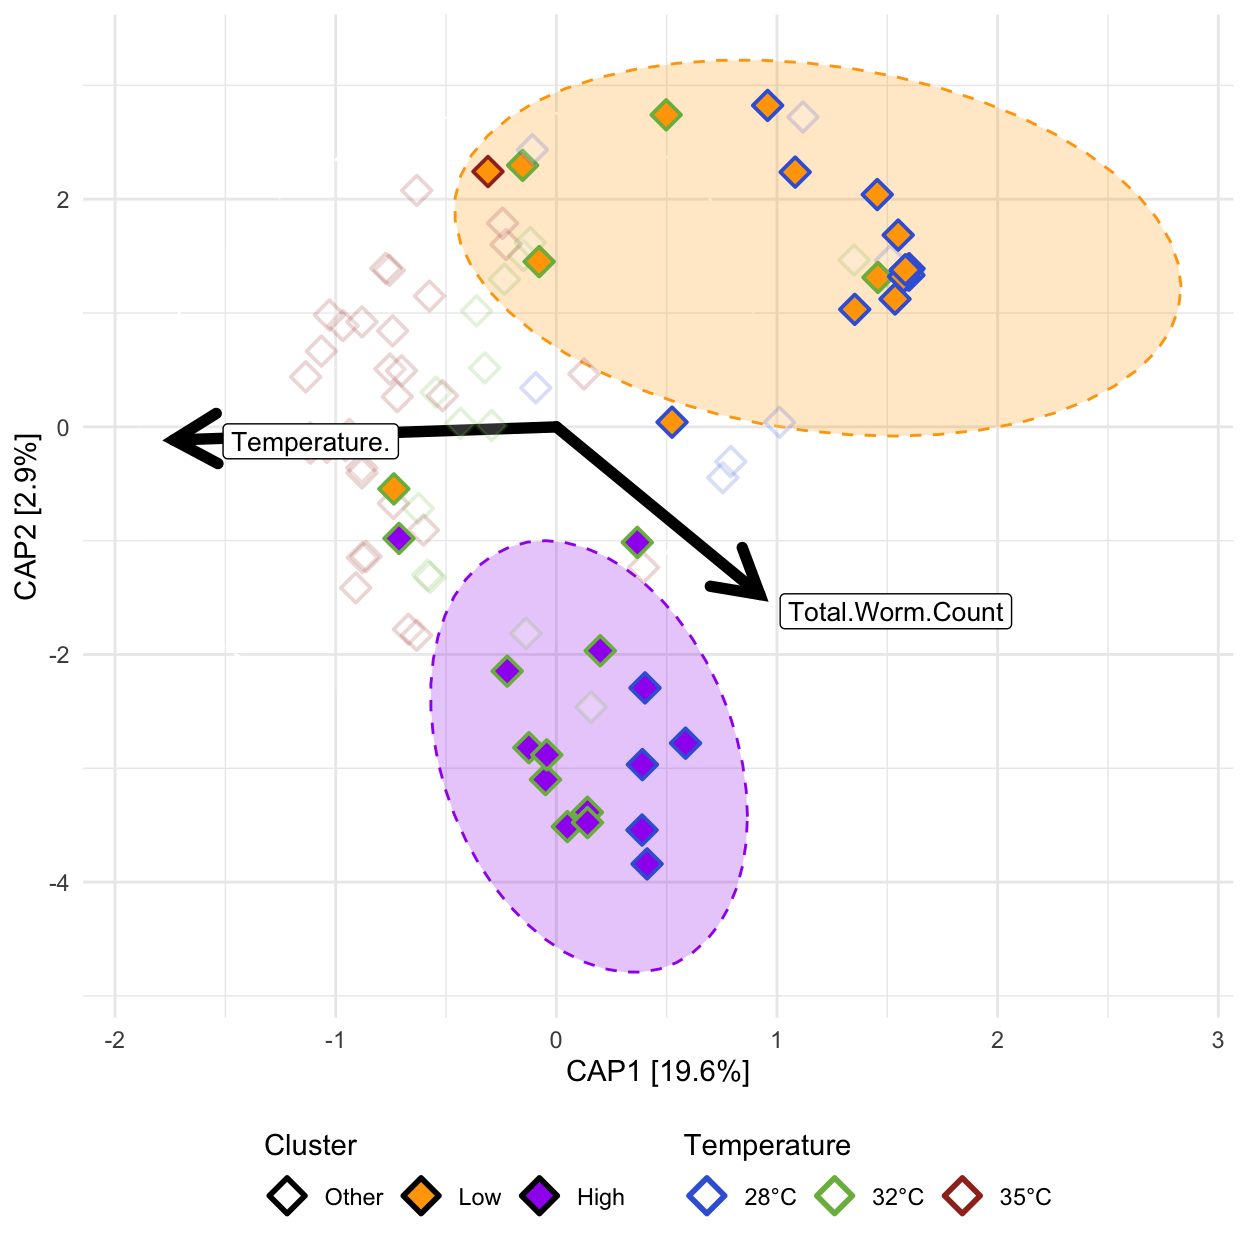
\includegraphics[keepaspectratio]{Results_Overview_files/figure-latex/plots-5D-1.pdf}}

\subparagraph{Tables}\label{tables-14}

(hide)

Click on tabs to display tables. Scroll to see additional rows.

ADONIS2

\begin{longtable}{lrrrrrl}
\caption*{
{\large ADONIS2} \\ 
{\small adonis2(Beta Distance \textasciitilde{} Temperature*Cluster); Exposed fish}
} \\ 
\toprule
term & df & SumOfSqs & R2 & statistic & p.value & sig \\ 
\midrule\addlinespace[2.5pt]
\multicolumn{7}{l}{bray} \\ 
\midrule\addlinespace[2.5pt]
Temperature & $2.000$ & $5.218$ & $0.251$ & $18.730$ & $0.001$ & *** \\ 
Cluster & $2.000$ & $3.594$ & $0.173$ & $12.902$ & $0.001$ & *** \\ 
Temperature:Cluster & $3.000$ & $0.653$ & $0.031$ & $1.564$ & $0.097$ & ns \\ 
Residual & $81.000$ & $11.282$ & $0.544$ & NA & NA & NA \\ 
Total & $88.000$ & $20.748$ & $1.000$ & NA & NA & NA \\ 
\midrule\addlinespace[2.5pt]
\multicolumn{7}{l}{canberra} \\ 
\midrule\addlinespace[2.5pt]
Temperature & $2.000$ & $3.573$ & $0.117$ & $6.064$ & $0.001$ & *** \\ 
Cluster & $2.000$ & $1.928$ & $0.063$ & $3.273$ & $0.001$ & *** \\ 
Temperature:Cluster & $3.000$ & $1.157$ & $0.038$ & $1.310$ & $0.052$ & ns \\ 
Residual & $81.000$ & $23.862$ & $0.782$ & NA & NA & NA \\ 
Total & $88.000$ & $30.520$ & $1.000$ & NA & NA & NA \\ 
\midrule\addlinespace[2.5pt]
\multicolumn{7}{l}{gunifrac} \\ 
\midrule\addlinespace[2.5pt]
Temperature & $2.000$ & $3.363$ & $0.212$ & $14.844$ & $0.001$ & *** \\ 
Cluster & $2.000$ & $2.657$ & $0.168$ & $11.728$ & $0.001$ & *** \\ 
Temperature:Cluster & $3.000$ & $0.645$ & $0.041$ & $1.898$ & $0.027$ & * \\ 
Residual & $81.000$ & $9.176$ & $0.579$ & NA & NA & NA \\ 
Total & $88.000$ & $15.841$ & $1.000$ & NA & NA & NA \\ 
\bottomrule
\end{longtable}

Dispersion (ANOVA)

\begin{longtable}{lrrrrrl}
\caption*{
{\large ANOVA: Homogeneity of Dispersion} \\ 
{\small ANOVA(Beta Disperson \textasciitilde{} Temperature*Cluster); Exposed fish}
} \\ 
\toprule
term & df & sumsq & meansq & statistic & p.value & sig \\ 
\midrule\addlinespace[2.5pt]
\multicolumn{7}{l}{bray} \\ 
\midrule\addlinespace[2.5pt]
Cluster & $2.000$ & $0.019$ & $0.009$ & $0.383$ & $\geq$0.25 & ns \\ 
Residual & $86.000$ & $2.116$ & $0.025$ & NA & NA & NA \\ 
\midrule\addlinespace[2.5pt]
\multicolumn{7}{l}{canberra} \\ 
\midrule\addlinespace[2.5pt]
Cluster & $2.000$ & $0.167$ & $0.084$ & $10.322$ & <0.001 & **** \\ 
Residual & $86.000$ & $0.697$ & $0.008$ & NA & NA & NA \\ 
\midrule\addlinespace[2.5pt]
\multicolumn{7}{l}{gunifrac} \\ 
\midrule\addlinespace[2.5pt]
Cluster & $2.000$ & $0.016$ & $0.008$ & $0.628$ & $\geq$0.25 & ns \\ 
Residual & $86.000$ & $1.078$ & $0.013$ & NA & NA & NA \\ 
\bottomrule
\end{longtable}

Dispersion (Tukey)

\begin{longtable}{llllrrrrl}
\caption*{
{\large Tukey: Homogeneity of Dispersion} \\ 
{\small Tukey(Beta Disperson \textasciitilde{} Temperature*Cluster); Exposed fish}
} \\ 
\toprule
.y. & term & group1 & group2 & estimate & conf.low & conf.high & adj.p.value & sig \\ 
\midrule\addlinespace[2.5pt]
\multicolumn{9}{l}{bray} \\ 
\midrule\addlinespace[2.5pt]
Distance & Cluster & Low & Other & $-0.037$ & $-0.138$ & $0.064$ & $\geq$0.25 & ns \\ 
Distance & Cluster & High & Other & $-0.005$ & $-0.114$ & $0.104$ & $\geq$0.25 & ns \\ 
Distance & Cluster & High & Low & $0.032$ & $-0.099$ & $0.163$ & $\geq$0.25 & ns \\ 
\midrule\addlinespace[2.5pt]
\multicolumn{9}{l}{canberra} \\ 
\midrule\addlinespace[2.5pt]
Distance & Cluster & Low & Other & $0.098$ & $0.040$ & $0.156$ & <0.001 & *** \\ 
Distance & Cluster & High & Other & $-0.031$ & $-0.093$ & $0.032$ & $\geq$0.25 & ns \\ 
Distance & Cluster & High & Low & $-0.129$ & $-0.204$ & $-0.053$ & <0.001 & *** \\ 
\midrule\addlinespace[2.5pt]
\multicolumn{9}{l}{gunifrac} \\ 
\midrule\addlinespace[2.5pt]
Distance & Cluster & Low & Other & $0.017$ & $-0.055$ & $0.089$ & $\geq$0.25 & ns \\ 
Distance & Cluster & High & Other & $-0.027$ & $-0.104$ & $0.051$ & $\geq$0.25 & ns \\ 
Distance & Cluster & High & Low & $-0.044$ & $-0.137$ & $0.050$ & $\geq$0.25 & ns \\ 
\bottomrule
\end{longtable}

\subparagraph{Addl. Metrics}\label{addl.-metrics-11}

\subsubsection{}\label{section-3}

\paragraph{(hide)}\label{hide-18}

Click on tabs to reveal figures displaying additional metrics.

\paragraph{S5A}\label{s5a}

\pandocbounded{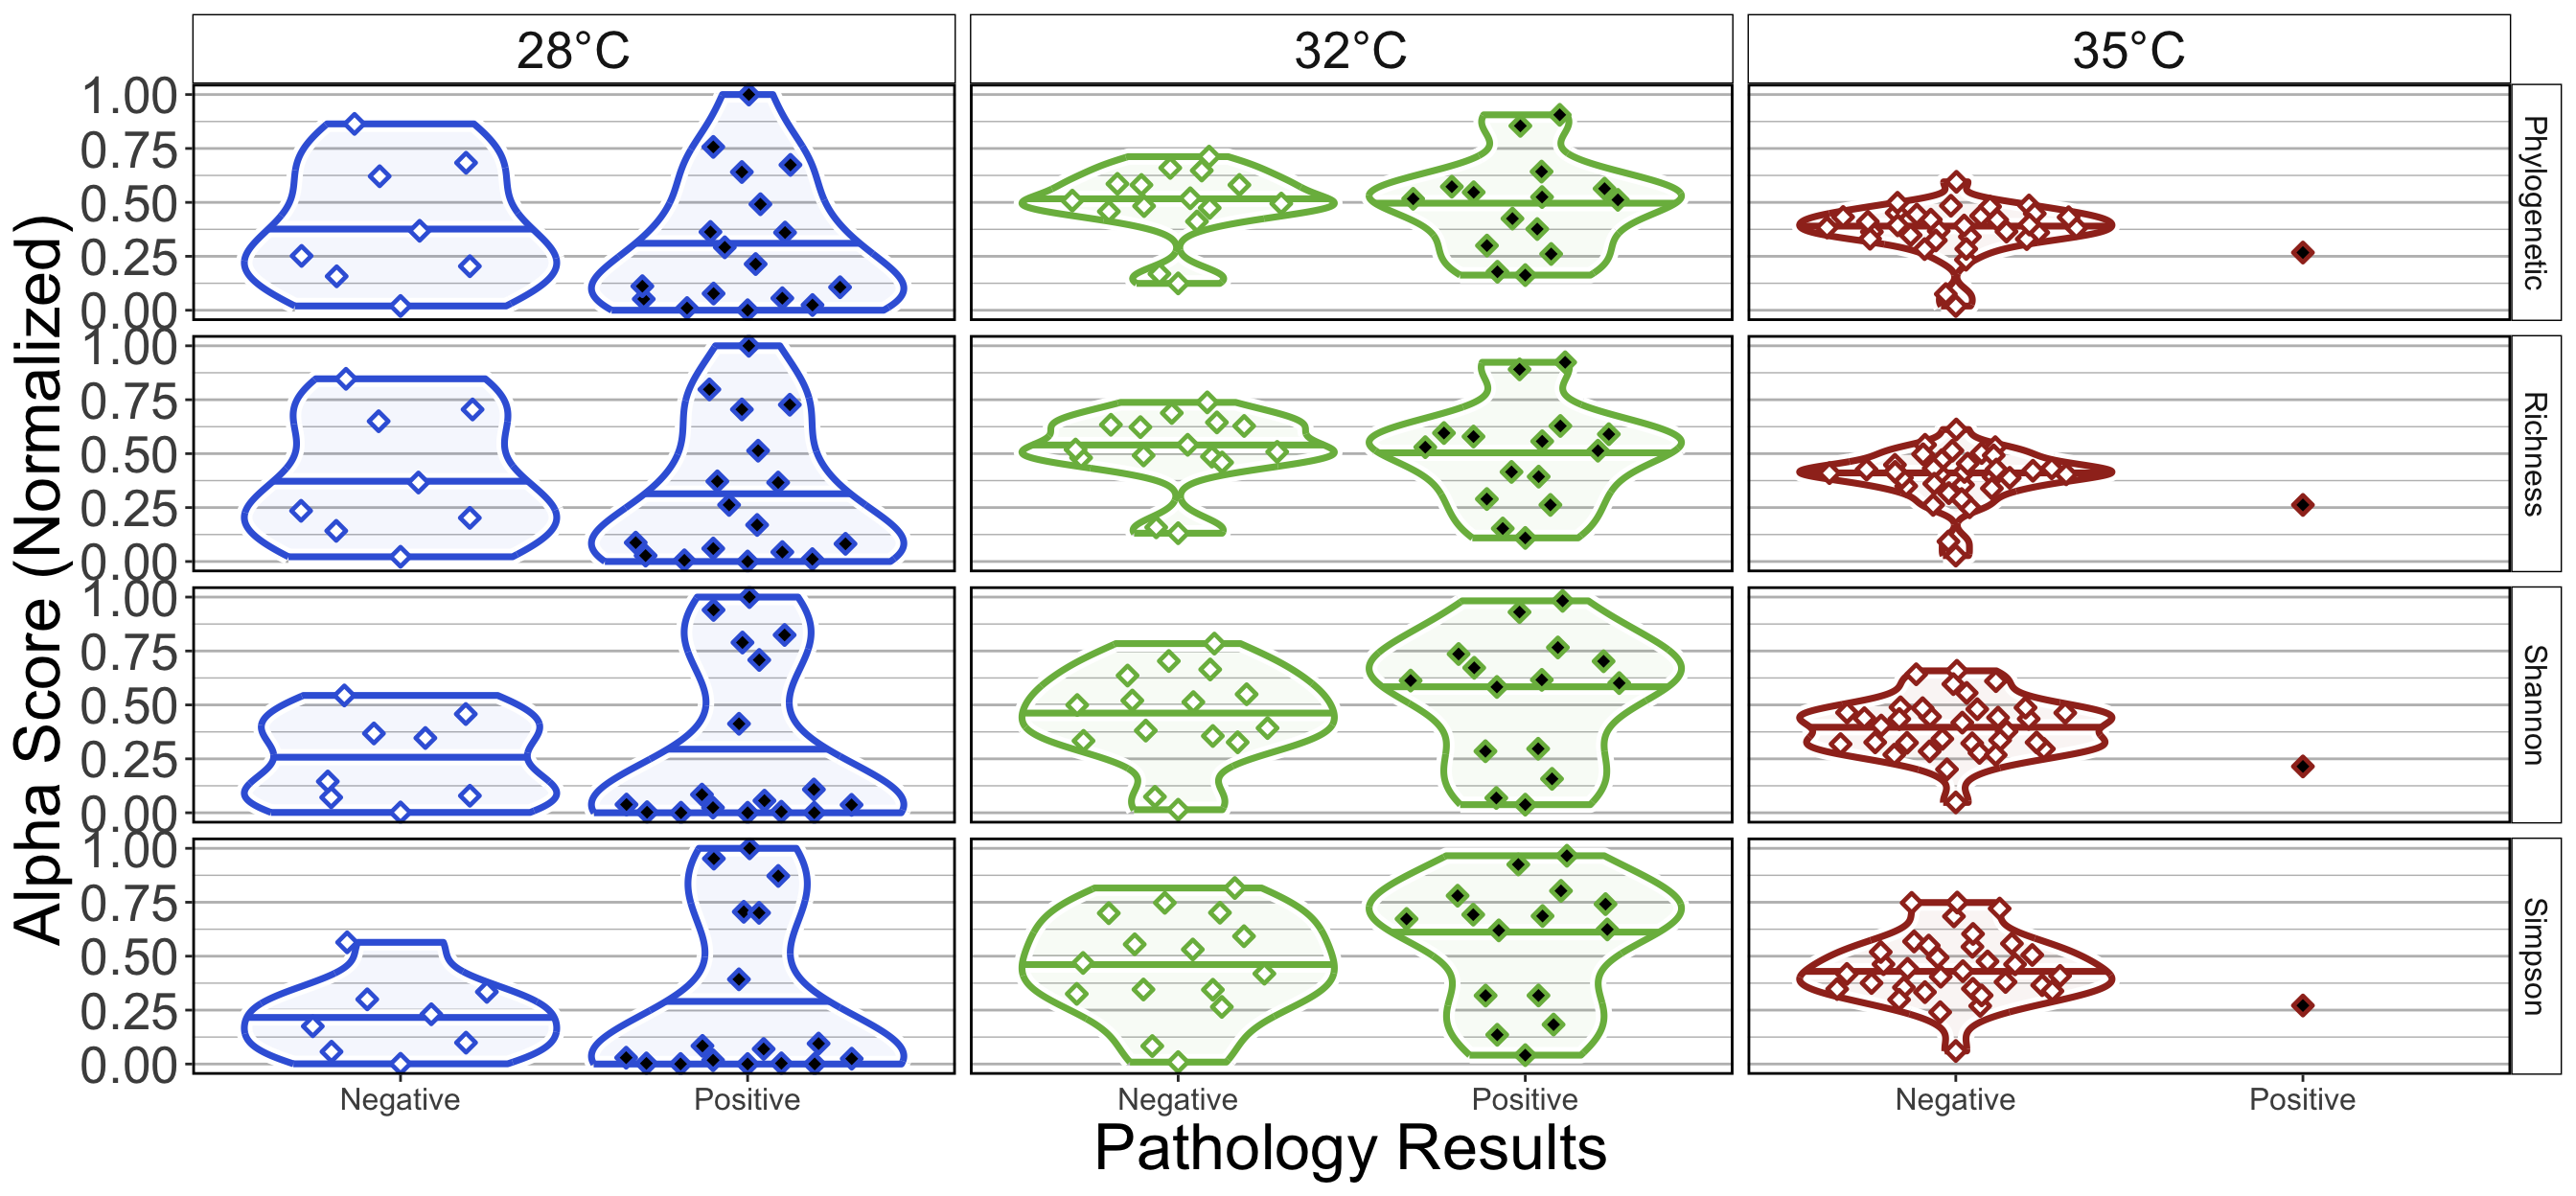
\includegraphics[keepaspectratio]{Results_Overview_files/figure-latex/plots-S5A-1.pdf}}

\paragraph{S5B}\label{s5b}

\pandocbounded{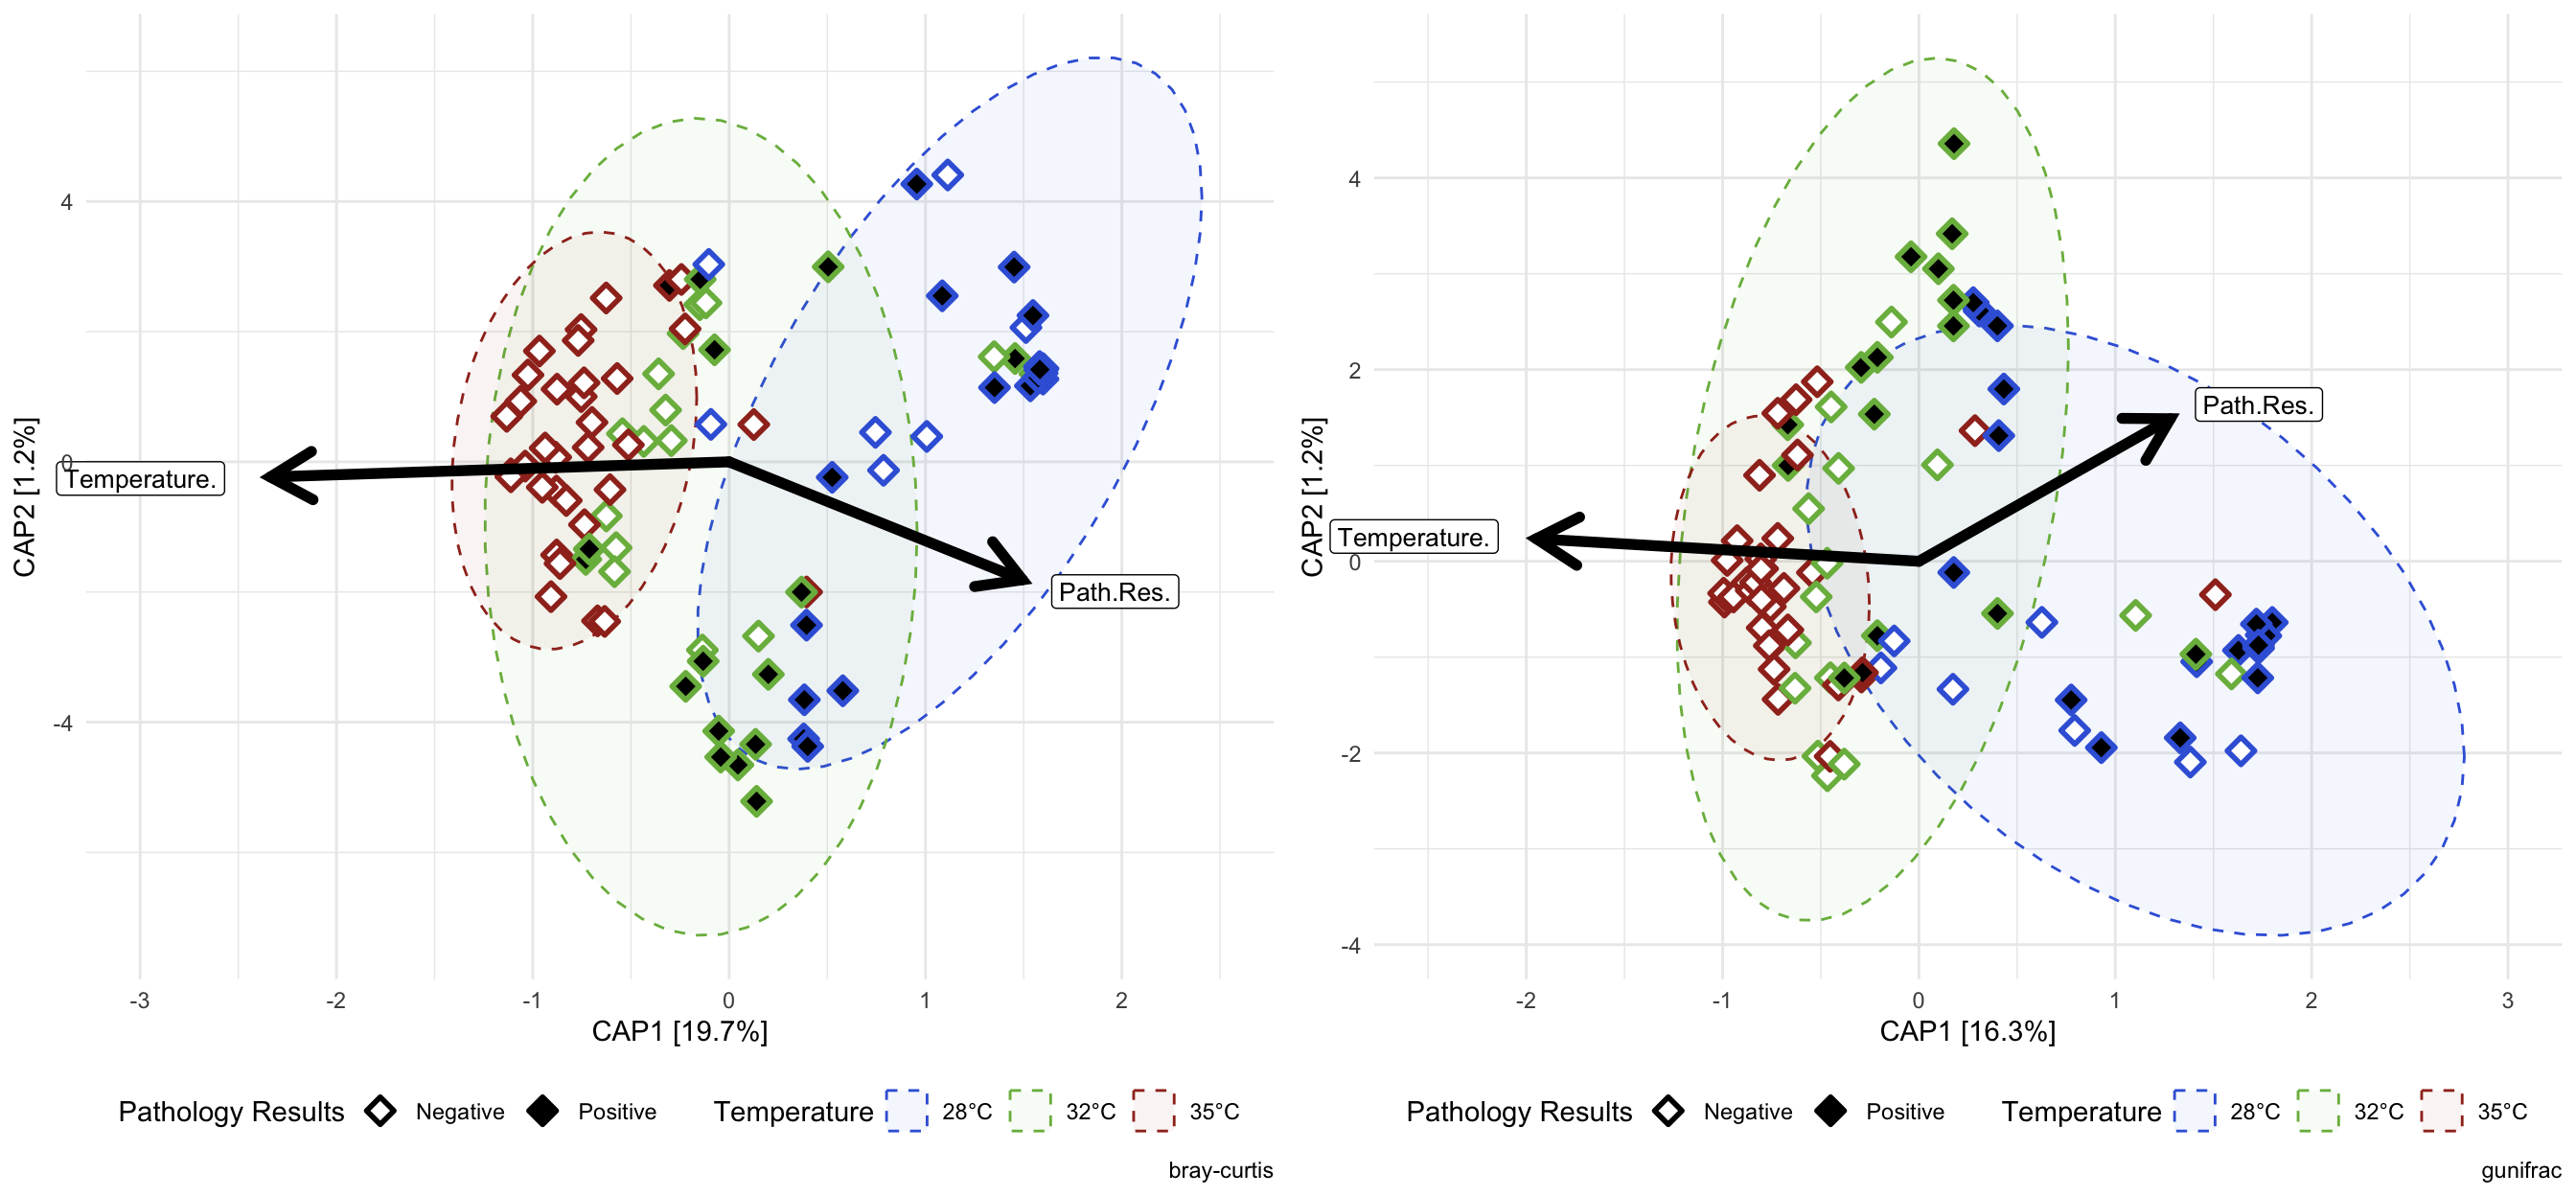
\includegraphics[keepaspectratio]{Results_Overview_files/figure-latex/plots-S5B-1.pdf}}

\paragraph{S5C}\label{s5c}

\pandocbounded{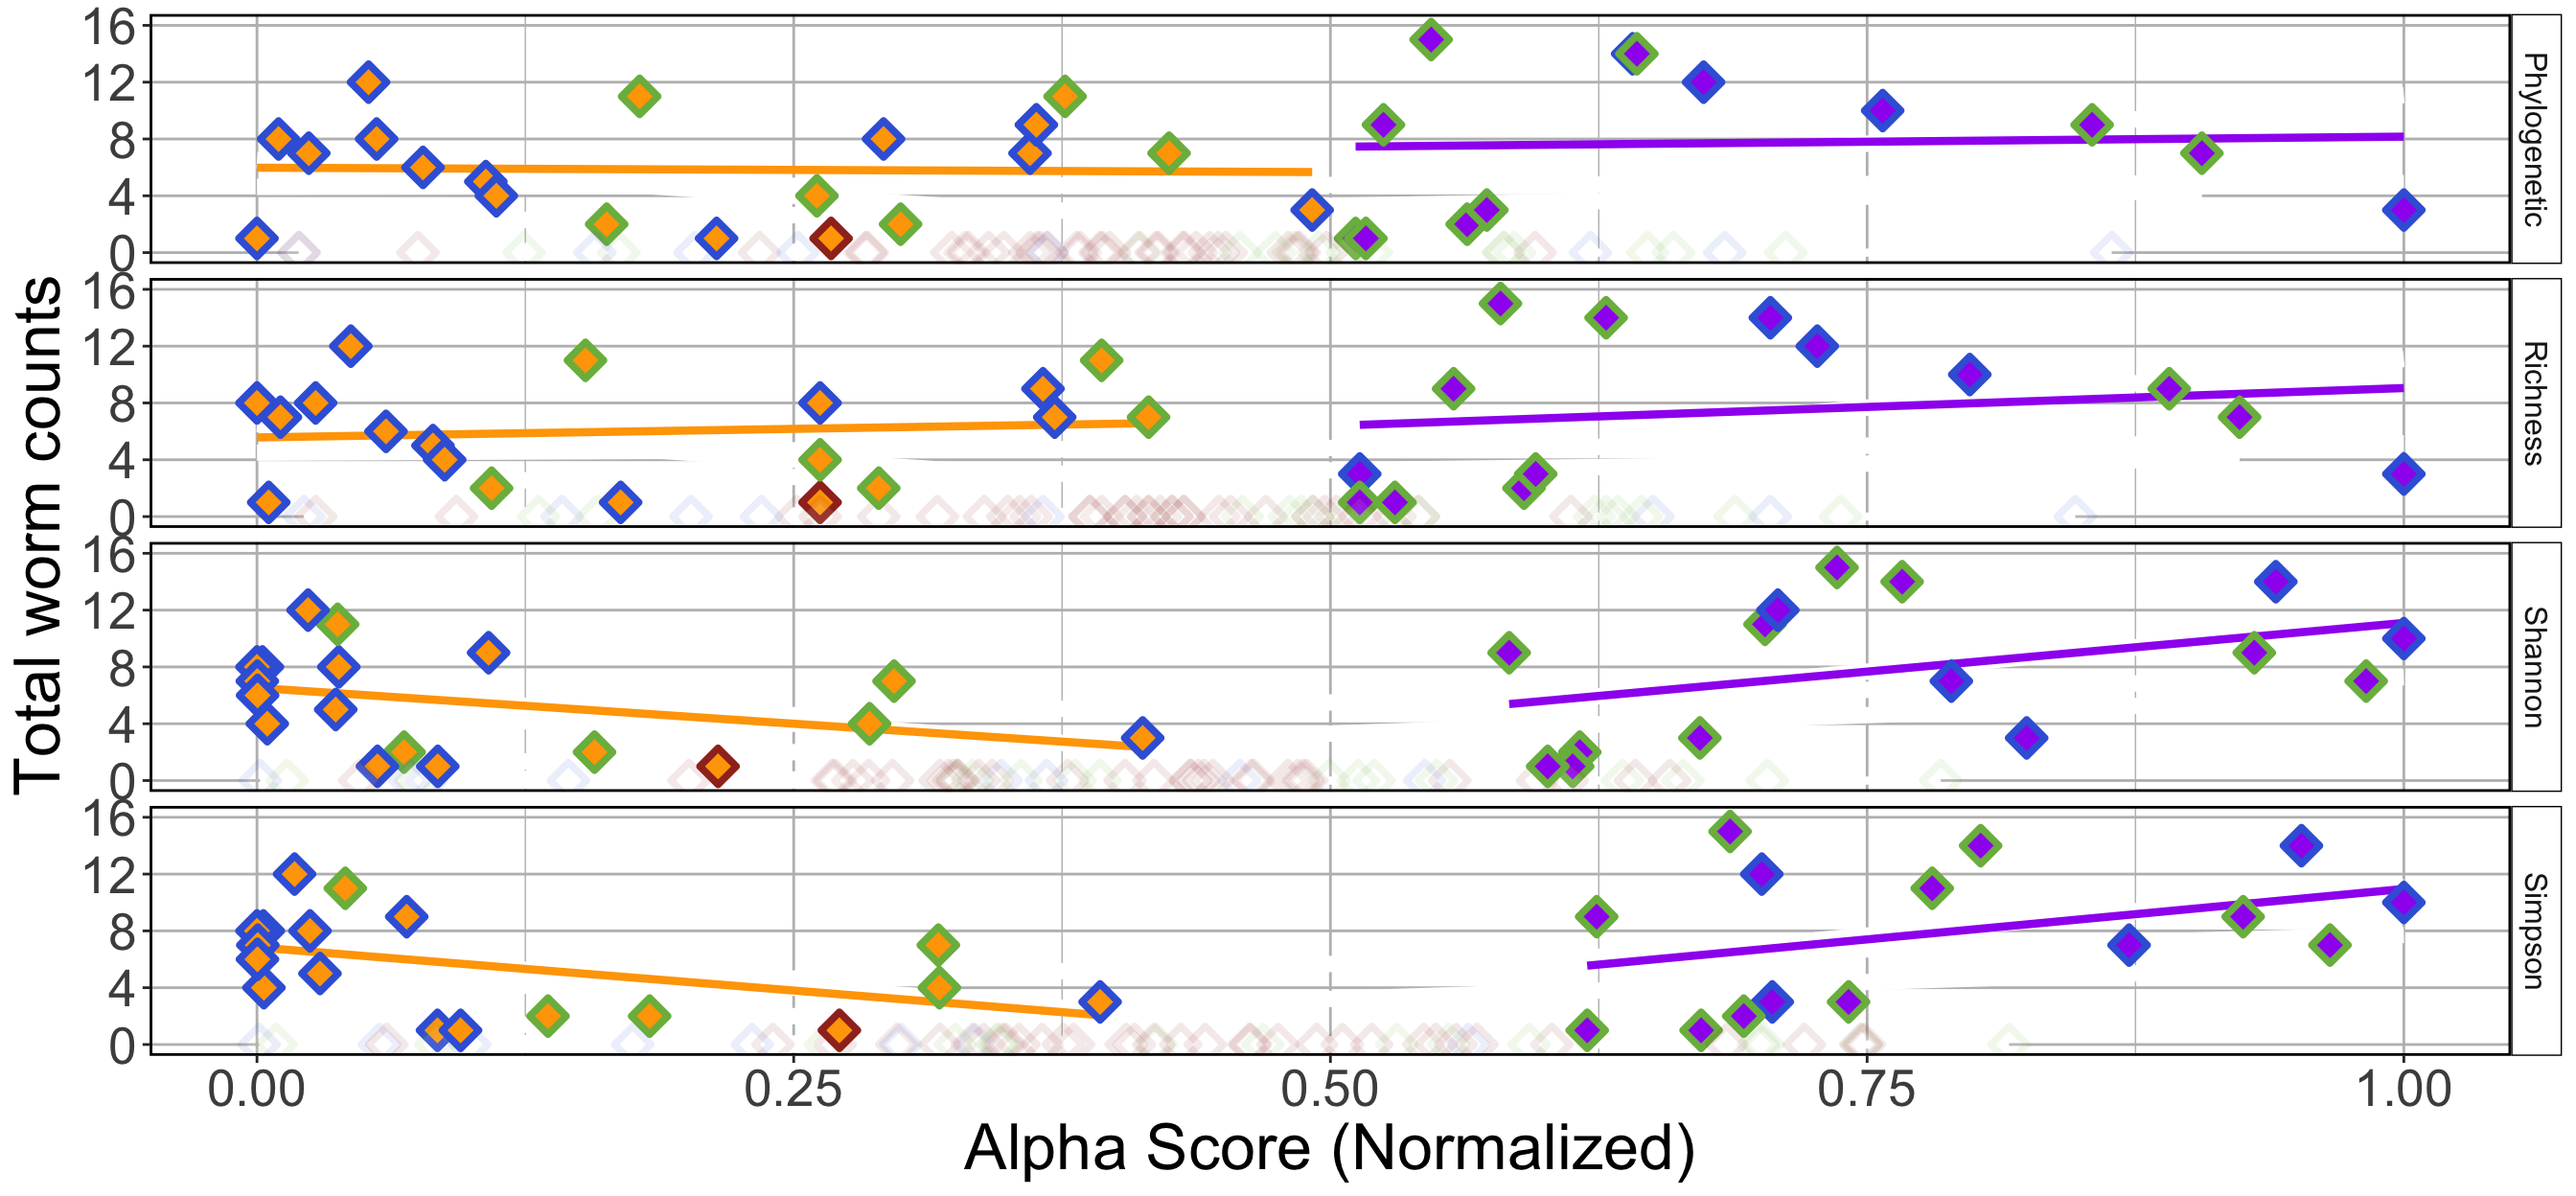
\includegraphics[keepaspectratio]{Results_Overview_files/figure-latex/plots-S5C-1.pdf}}

\paragraph{S5D}\label{s5d}

Click on tabs to cycle through different cluster comparisons between
alpha and beta diversity.

\subparagraph{Phylogenetic}\label{phylogenetic}

\pandocbounded{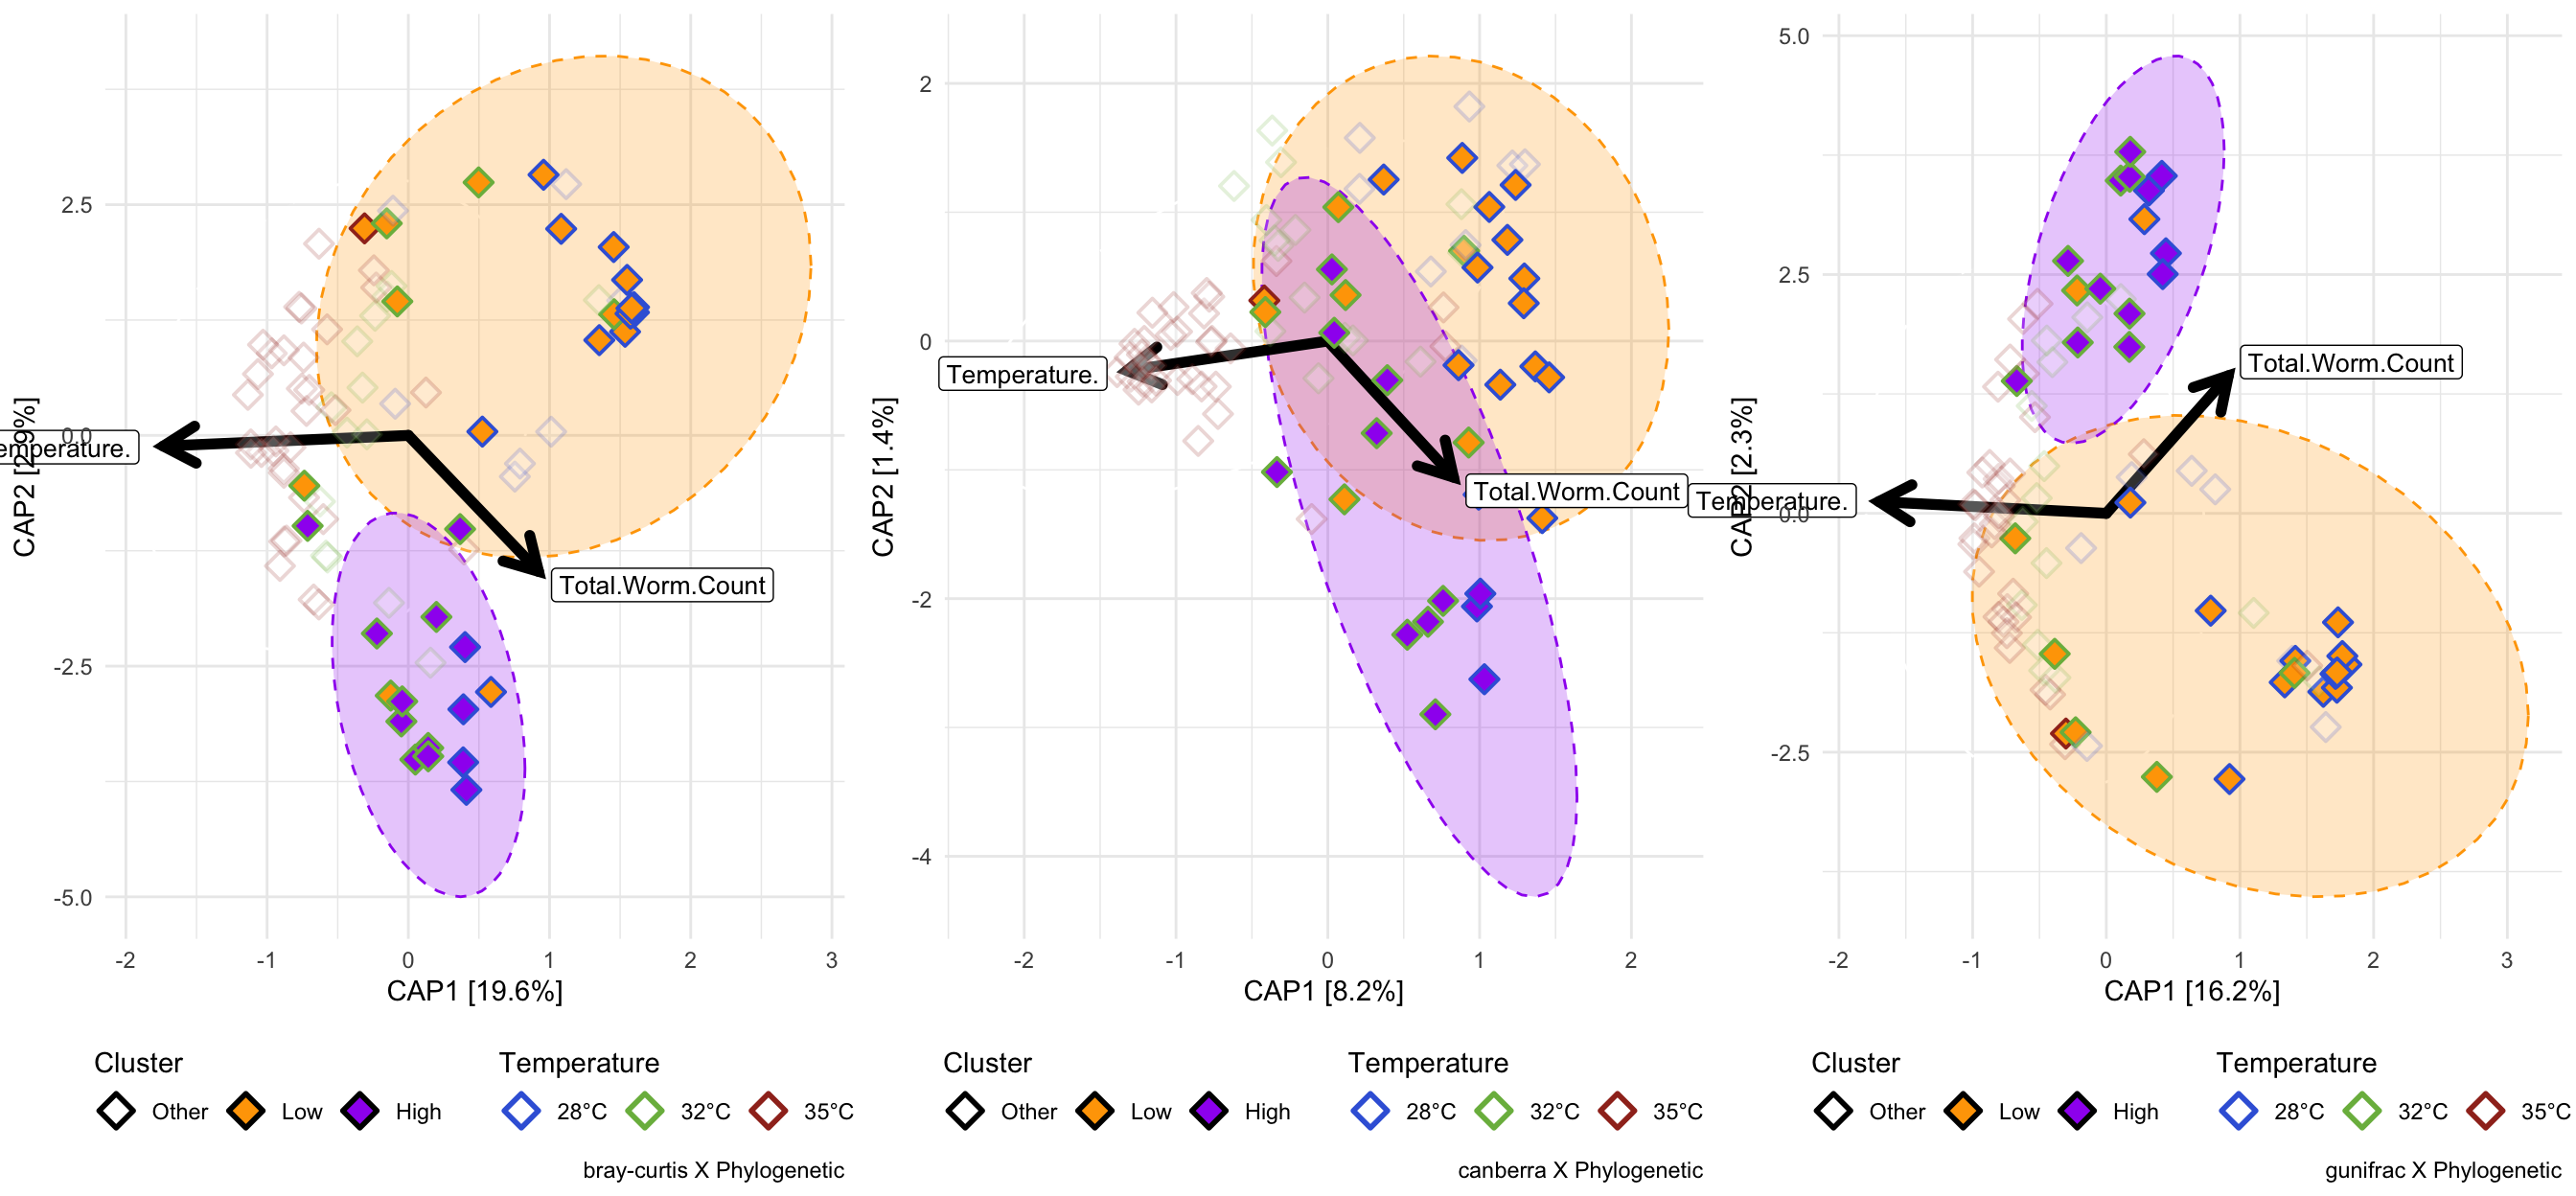
\includegraphics[keepaspectratio]{Results_Overview_files/figure-latex/plots-S5D-phylogenetic-1.pdf}}

\begin{longtable}{llrrrrrr}
\caption*{
{\large ADONIS2} \\ 
{\small adonis2(Beta Distance \textasciitilde{} Cluster); Exposed fish}
} \\ 
\toprule
Beta.Metric & term & df & SumOfSqs & R2 & statistic & p.value & p.adj.sig \\ 
\midrule\addlinespace[2.5pt]
\multicolumn{8}{l}{Phylogenetic} \\ 
\midrule\addlinespace[2.5pt]
bray & Cluster & $2.000$ & $5.369$ & $0.259$ & $15.012$ & $0.001$ & ** \\ 
bray & Residual & $86.000$ & $15.379$ & $0.741$ & NA & NA & NA \\ 
bray & Total & $88.000$ & $20.748$ & $1.000$ & NA & NA & NA \\ 
canberra & Cluster & $2.000$ & $3.204$ & $0.105$ & $5.043$ & $0.001$ & ** \\ 
canberra & Residual & $86.000$ & $27.317$ & $0.895$ & NA & NA & NA \\ 
canberra & Total & $88.000$ & $30.520$ & $1.000$ & NA & NA & NA \\ 
gunifrac & Cluster & $2.000$ & $3.692$ & $0.233$ & $13.068$ & $0.001$ & ** \\ 
gunifrac & Residual & $86.000$ & $12.149$ & $0.767$ & NA & NA & NA \\ 
gunifrac & Total & $88.000$ & $15.841$ & $1.000$ & NA & NA & NA \\ 
\bottomrule
\end{longtable}
\begin{longtable}{llrrrrrl}
\caption*{
{\large ANOVA: Homogeneity of Dispersion} \\ 
{\small ANOVA(Beta Disperson \textasciitilde{} Cluster); Exposed fish}
} \\ 
\toprule
Beta.Metric & term & df & sumsq & meansq & statistic & p.value & p.adj.sig \\ 
\midrule\addlinespace[2.5pt]
\multicolumn{8}{l}{Phylogenetic} \\ 
\midrule\addlinespace[2.5pt]
bray & Groups & $2.000$ & $0.039$ & $0.019$ & $0.754$ & $\geq$0.25 & ns \\ 
bray & Residuals & $86.000$ & $2.218$ & $0.026$ & NA & NA & NA \\ 
canberra & Groups & $2.000$ & $0.221$ & $0.110$ & $14.247$ & <0.001 & **** \\ 
canberra & Residuals & $86.000$ & $0.666$ & $0.008$ & NA & NA & NA \\ 
gunifrac & Groups & $2.000$ & $0.072$ & $0.036$ & $2.725$ & $0.071$ & ns \\ 
gunifrac & Residuals & $86.000$ & $1.131$ & $0.013$ & NA & NA & NA \\ 
\bottomrule
\end{longtable}

\subparagraph{Richness}\label{richness}

\pandocbounded{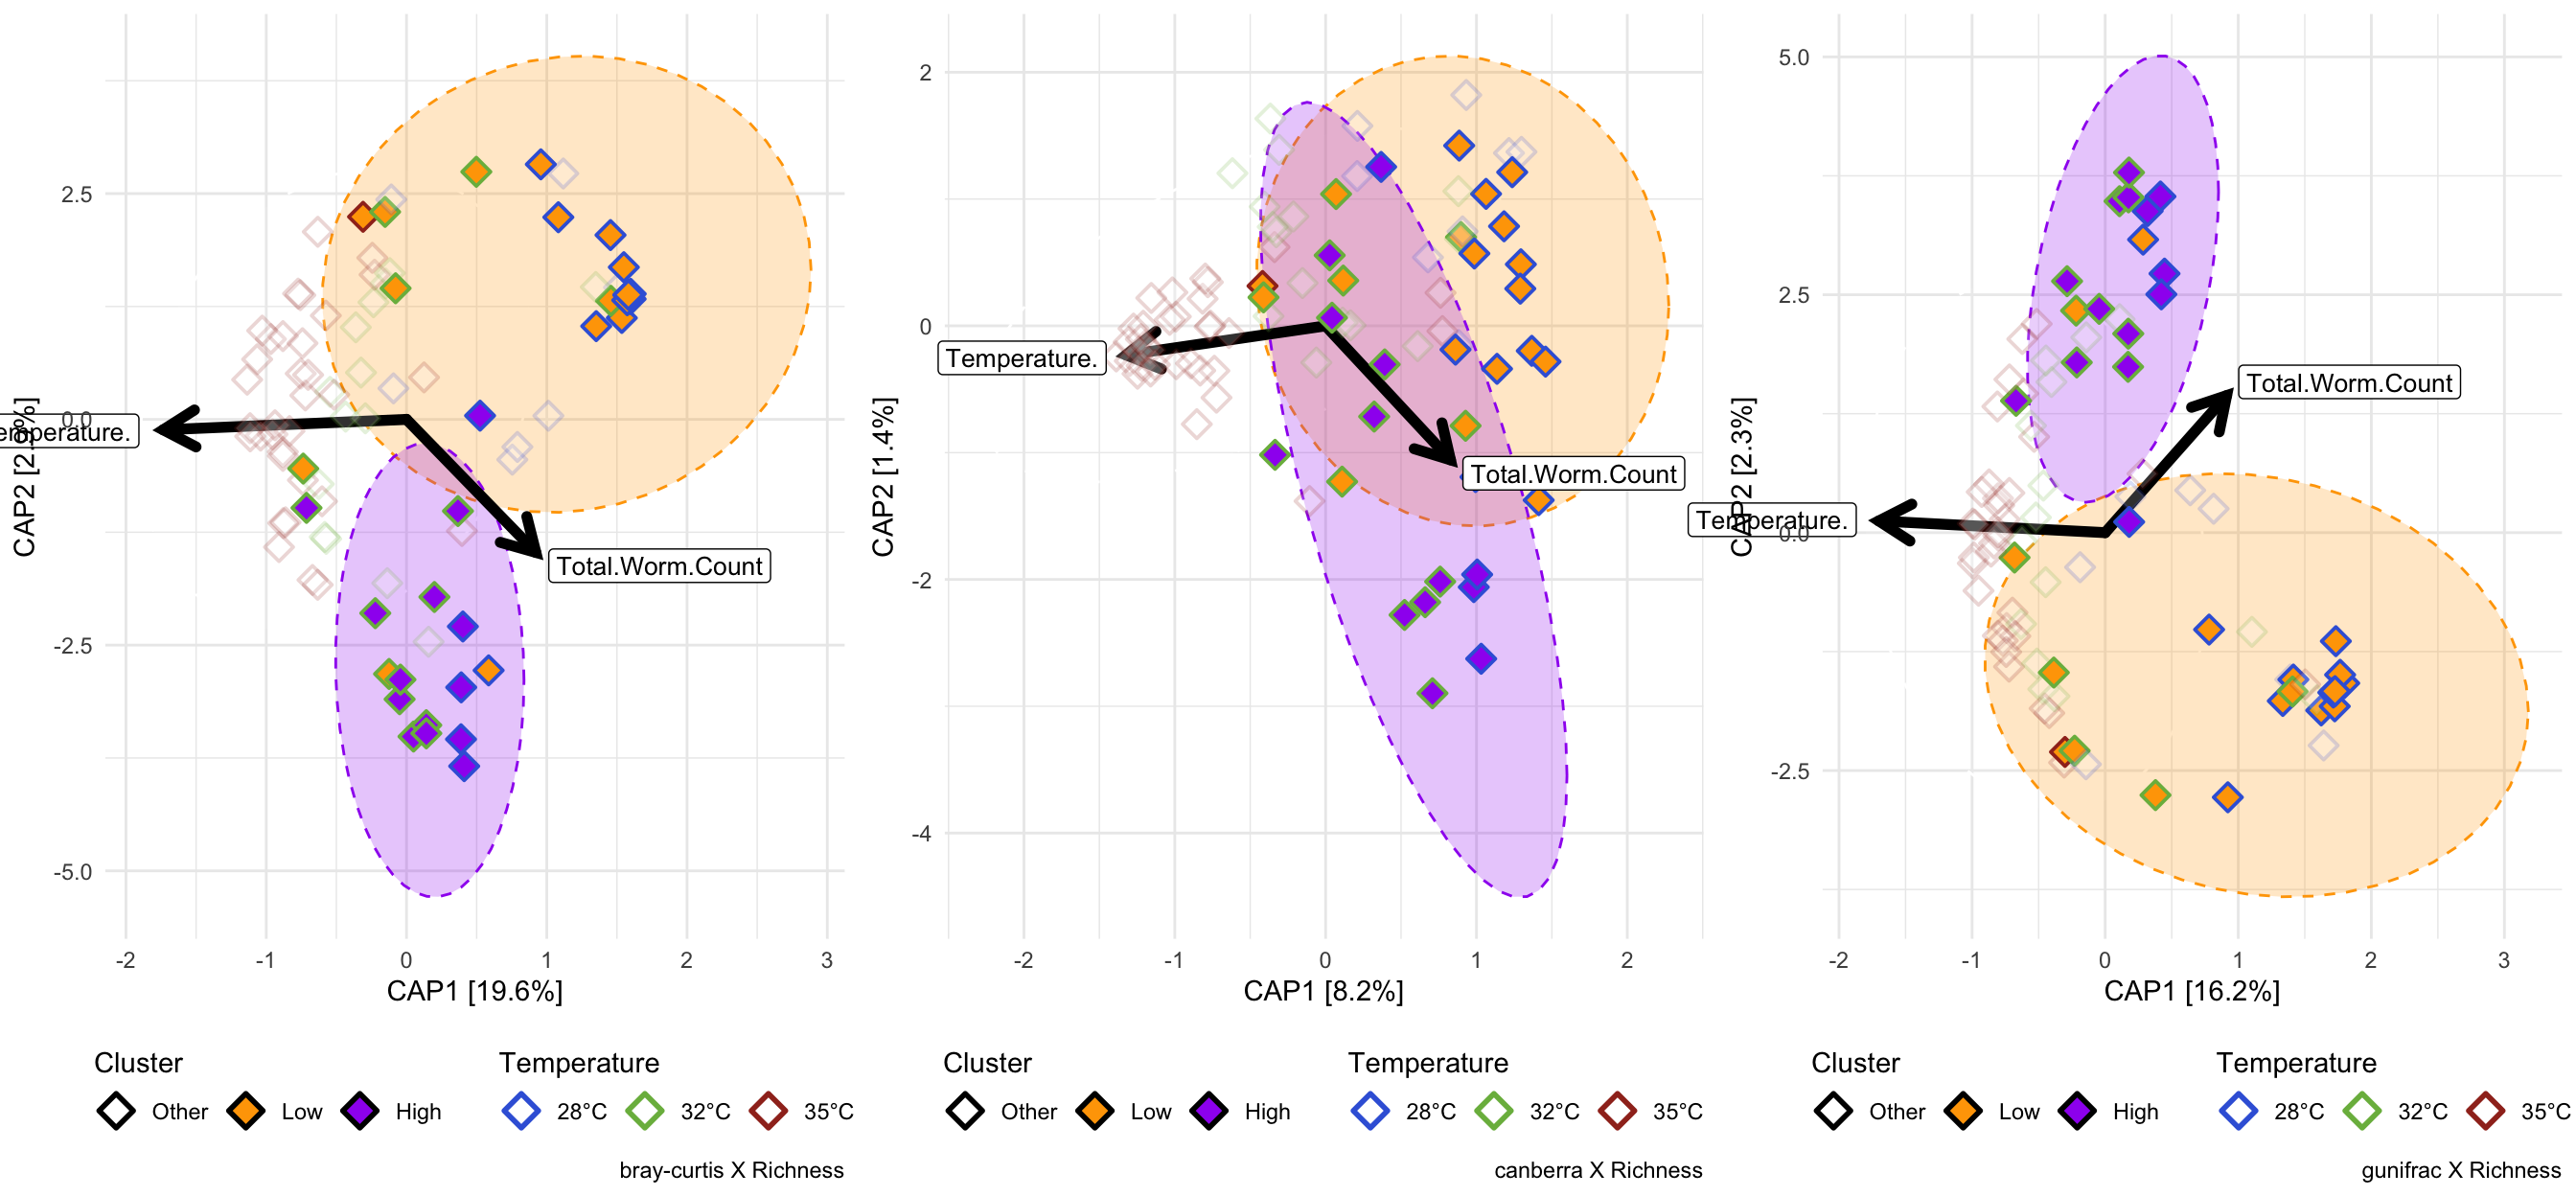
\includegraphics[keepaspectratio]{Results_Overview_files/figure-latex/plots-S5D-richness-1.pdf}}

\begin{longtable}{llrrrrrr}
\caption*{
{\large ADONIS2} \\ 
{\small adonis2(Beta Distance \textasciitilde{} Cluster); Exposed fish}
} \\ 
\toprule
Beta.Metric & term & df & SumOfSqs & R2 & statistic & p.value & p.adj.sig \\ 
\midrule\addlinespace[2.5pt]
\multicolumn{8}{l}{Richness} \\ 
\midrule\addlinespace[2.5pt]
bray & Cluster & $2.000$ & $5.363$ & $0.258$ & $14.990$ & $0.001$ & ** \\ 
bray & Residual & $86.000$ & $15.385$ & $0.742$ & NA & NA & NA \\ 
bray & Total & $88.000$ & $20.748$ & $1.000$ & NA & NA & NA \\ 
canberra & Cluster & $2.000$ & $3.356$ & $0.110$ & $5.312$ & $0.001$ & ** \\ 
canberra & Residual & $86.000$ & $27.165$ & $0.890$ & NA & NA & NA \\ 
canberra & Total & $88.000$ & $30.520$ & $1.000$ & NA & NA & NA \\ 
gunifrac & Cluster & $2.000$ & $3.835$ & $0.242$ & $13.736$ & $0.001$ & ** \\ 
gunifrac & Residual & $86.000$ & $12.006$ & $0.758$ & NA & NA & NA \\ 
gunifrac & Total & $88.000$ & $15.841$ & $1.000$ & NA & NA & NA \\ 
\bottomrule
\end{longtable}
\begin{longtable}{llrrrrrl}
\caption*{
{\large ANOVA: Homogeneity of Dispersion} \\ 
{\small ANOVA(Beta Disperson \textasciitilde{} Cluster); Exposed fish}
} \\ 
\toprule
Beta.Metric & term & df & sumsq & meansq & statistic & p.value & p.adj.sig \\ 
\midrule\addlinespace[2.5pt]
\multicolumn{8}{l}{Richness} \\ 
\midrule\addlinespace[2.5pt]
bray & Groups & $2.000$ & $0.028$ & $0.014$ & $0.535$ & $\geq$0.25 & ns \\ 
bray & Residuals & $86.000$ & $2.263$ & $0.026$ & NA & NA & NA \\ 
canberra & Groups & $2.000$ & $0.216$ & $0.108$ & $13.957$ & <0.001 & **** \\ 
canberra & Residuals & $86.000$ & $0.664$ & $0.008$ & NA & NA & NA \\ 
gunifrac & Groups & $2.000$ & $0.050$ & $0.025$ & $1.873$ & $0.160$ & ns \\ 
gunifrac & Residuals & $86.000$ & $1.155$ & $0.013$ & NA & NA & NA \\ 
\bottomrule
\end{longtable}

\subparagraph{Shannon}\label{shannon}

\pandocbounded{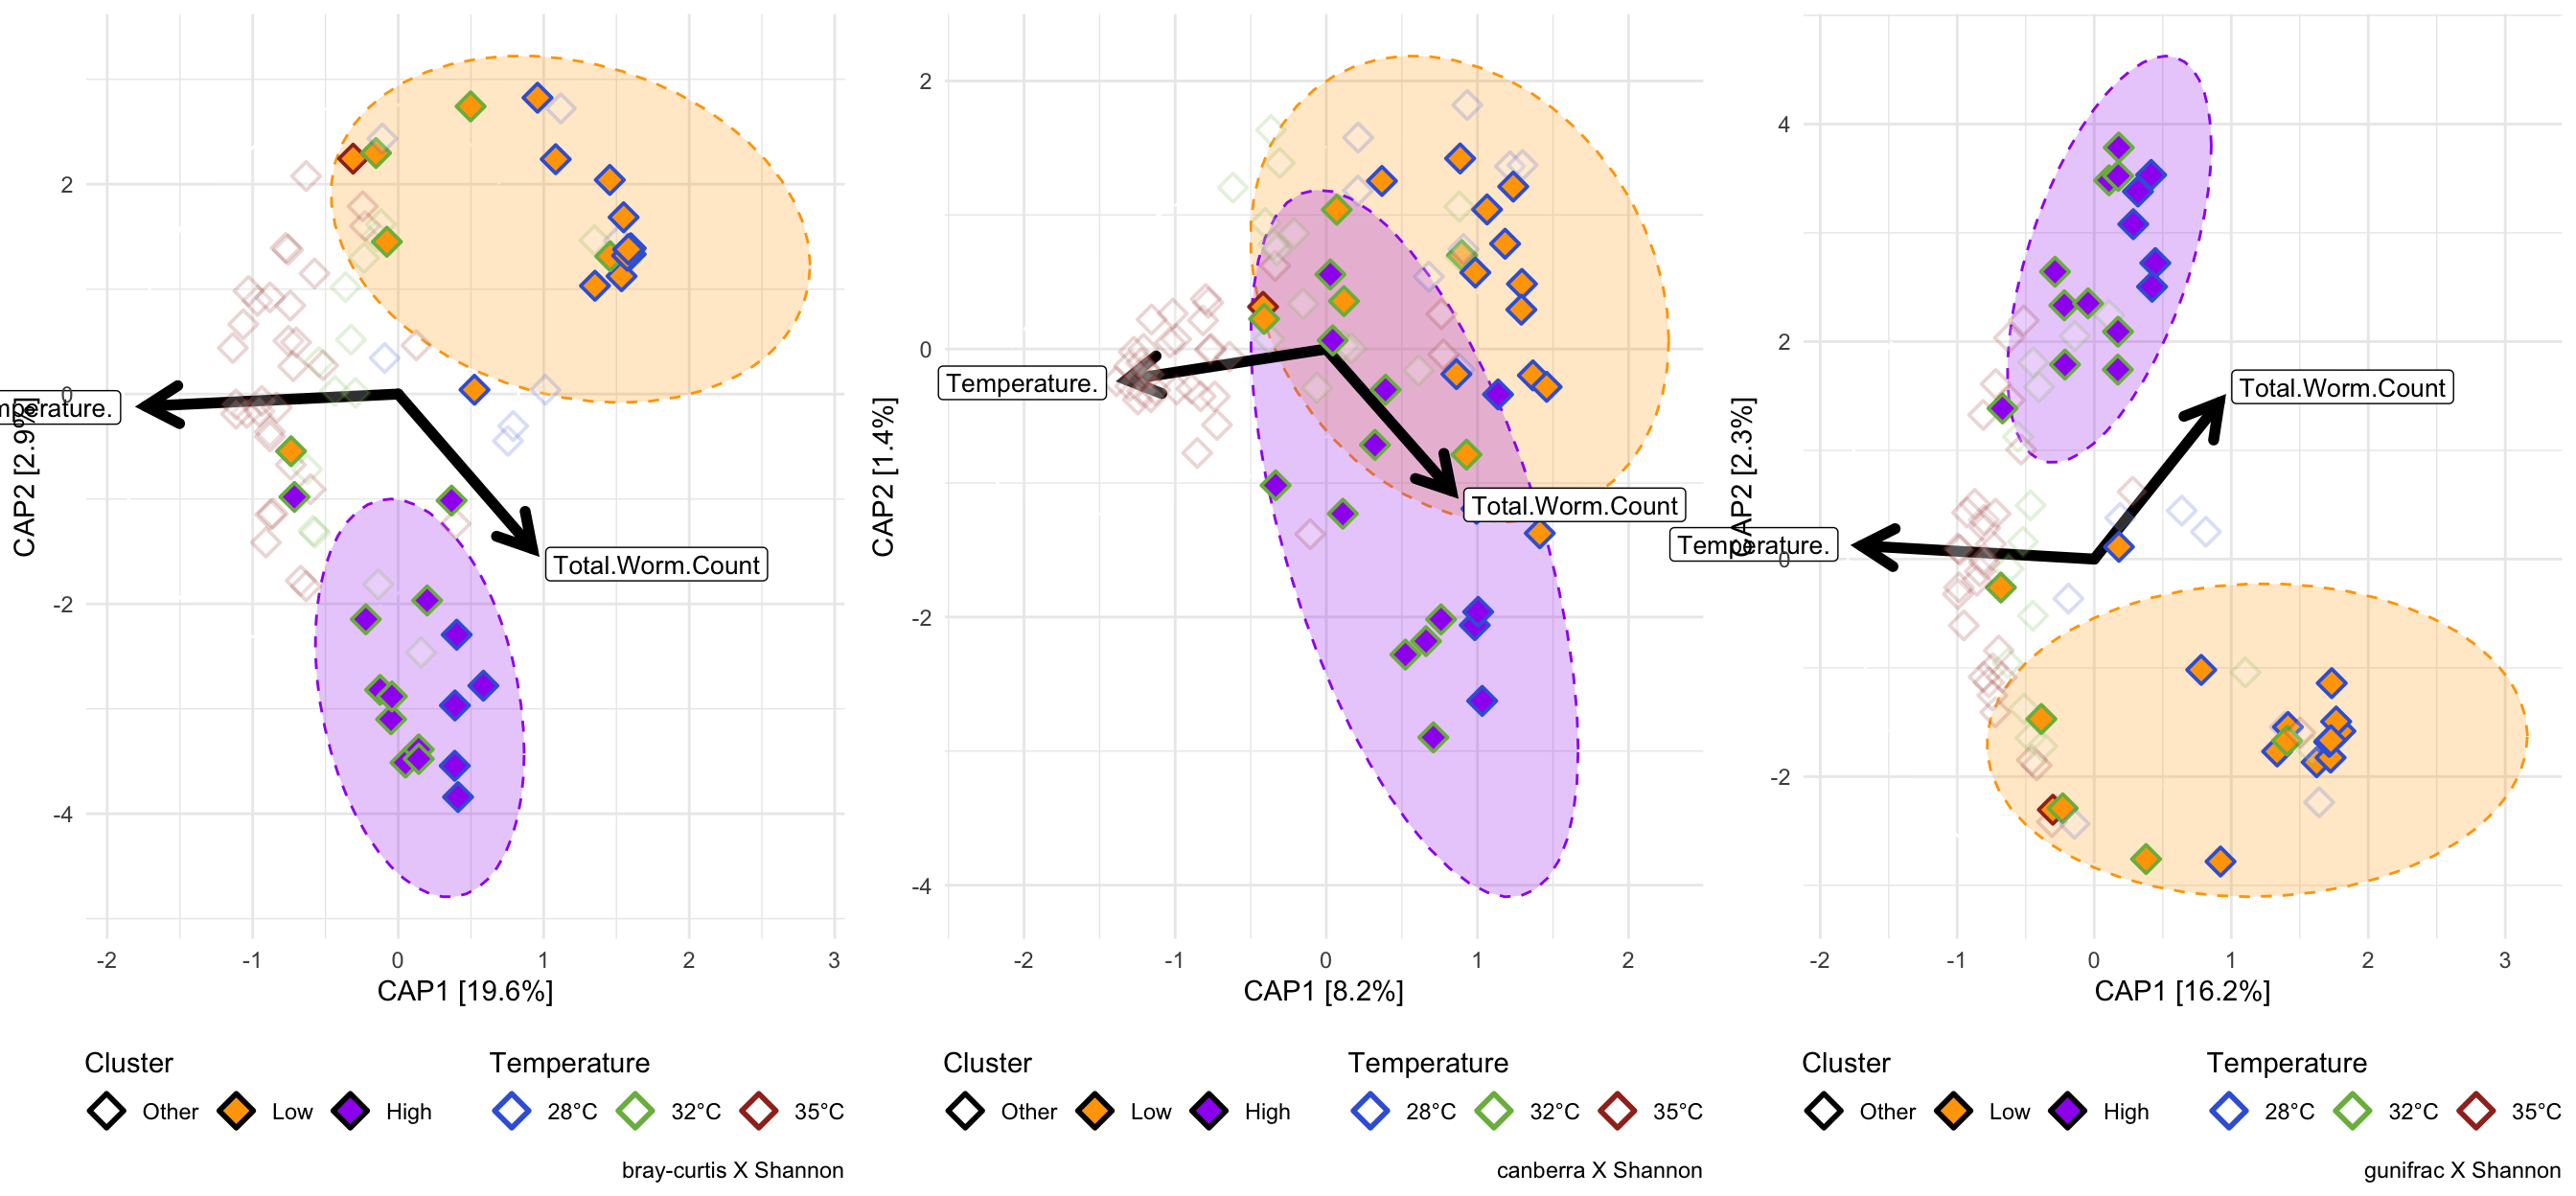
\includegraphics[keepaspectratio]{Results_Overview_files/figure-latex/plots-S5D-shannon-1.pdf}}

\begin{longtable}{llrrrrrr}
\caption*{
{\large ADONIS2} \\ 
{\small adonis2(Beta Distance \textasciitilde{} Cluster); Exposed fish}
} \\ 
\toprule
Beta.Metric & term & df & SumOfSqs & R2 & statistic & p.value & p.adj.sig \\ 
\midrule\addlinespace[2.5pt]
\multicolumn{8}{l}{Shannon} \\ 
\midrule\addlinespace[2.5pt]
bray & Cluster & $2.000$ & $5.943$ & $0.286$ & $17.260$ & $0.001$ & ** \\ 
bray & Residual & $86.000$ & $14.805$ & $0.714$ & NA & NA & NA \\ 
bray & Total & $88.000$ & $20.748$ & $1.000$ & NA & NA & NA \\ 
canberra & Cluster & $2.000$ & $3.188$ & $0.104$ & $5.016$ & $0.001$ & ** \\ 
canberra & Residual & $86.000$ & $27.332$ & $0.896$ & NA & NA & NA \\ 
canberra & Total & $88.000$ & $30.520$ & $1.000$ & NA & NA & NA \\ 
gunifrac & Cluster & $2.000$ & $4.229$ & $0.267$ & $15.660$ & $0.001$ & ** \\ 
gunifrac & Residual & $86.000$ & $11.612$ & $0.733$ & NA & NA & NA \\ 
gunifrac & Total & $88.000$ & $15.841$ & $1.000$ & NA & NA & NA \\ 
\bottomrule
\end{longtable}
\begin{longtable}{llrrrrrl}
\caption*{
{\large ANOVA: Homogeneity of Dispersion} \\ 
{\small ANOVA(Beta Disperson \textasciitilde{} Cluster); Exposed fish}
} \\ 
\toprule
Beta.Metric & term & df & sumsq & meansq & statistic & p.value & p.adj.sig \\ 
\midrule\addlinespace[2.5pt]
\multicolumn{8}{l}{Shannon} \\ 
\midrule\addlinespace[2.5pt]
bray & Groups & $2.000$ & $0.019$ & $0.009$ & $0.383$ & $\geq$0.25 & ns \\ 
bray & Residuals & $86.000$ & $2.116$ & $0.025$ & NA & NA & NA \\ 
canberra & Groups & $2.000$ & $0.167$ & $0.084$ & $10.322$ & <0.001 & **** \\ 
canberra & Residuals & $86.000$ & $0.697$ & $0.008$ & NA & NA & NA \\ 
gunifrac & Groups & $2.000$ & $0.016$ & $0.008$ & $0.628$ & $\geq$0.25 & ns \\ 
gunifrac & Residuals & $86.000$ & $1.078$ & $0.013$ & NA & NA & NA \\ 
\bottomrule
\end{longtable}

\subparagraph{Simpsons}\label{simpsons}

\pandocbounded{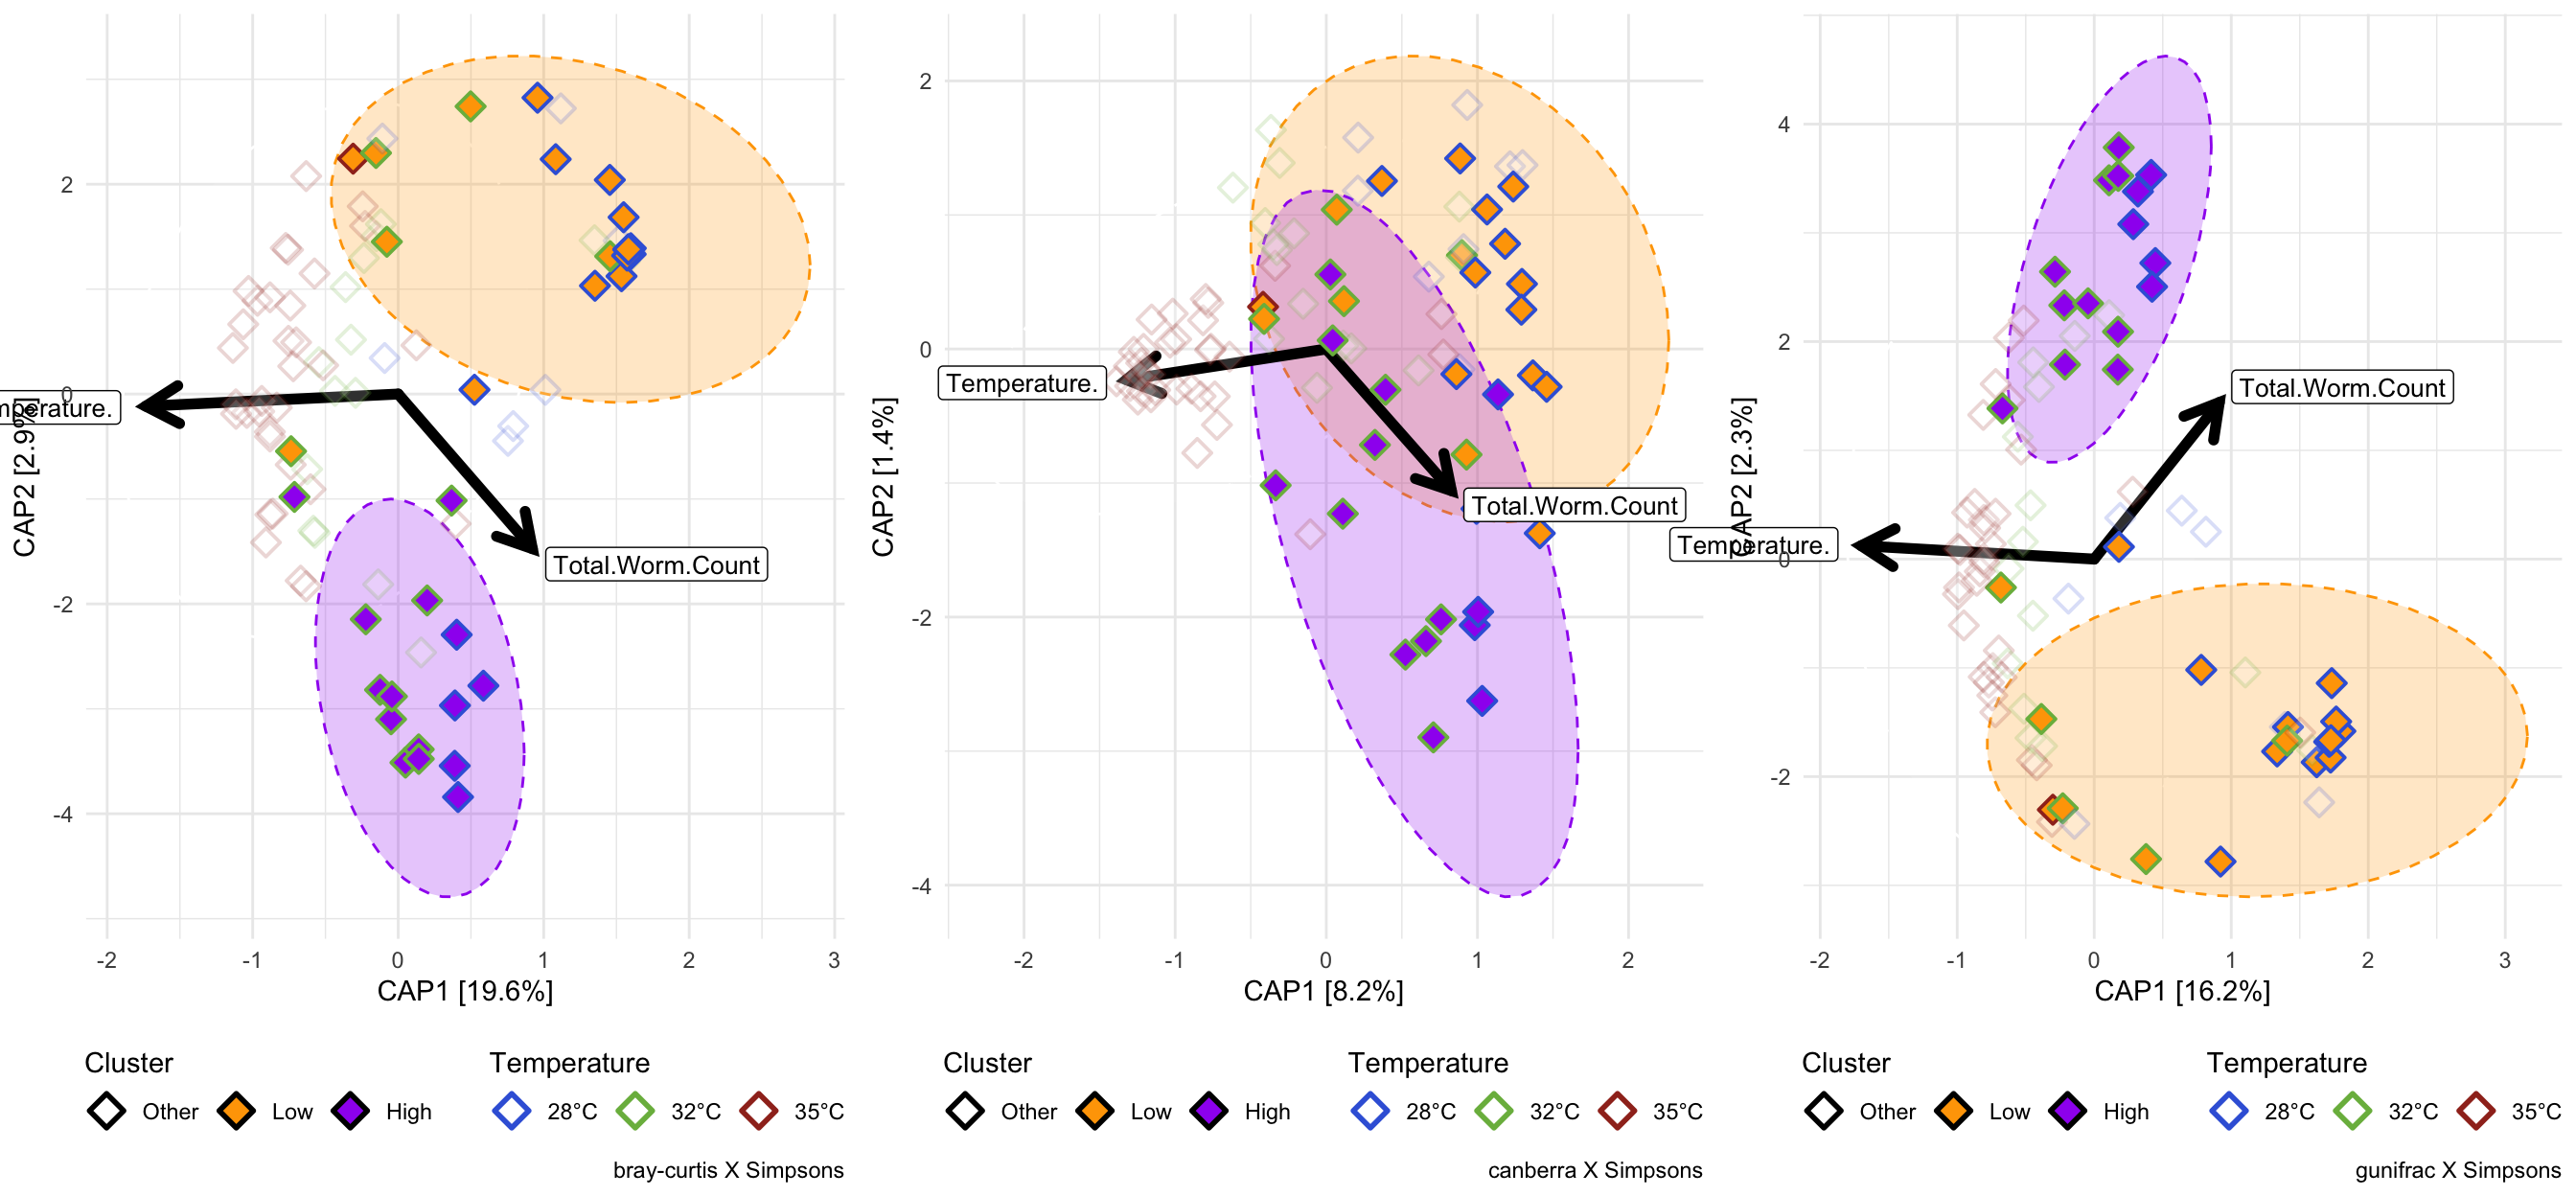
\includegraphics[keepaspectratio]{Results_Overview_files/figure-latex/plots-S5D-simpsons-1.pdf}}

\begin{longtable}{llrrrrrr}
\caption*{
{\large ADONIS2} \\ 
{\small adonis2(Beta Distance \textasciitilde{} Cluster); Exposed fish}
} \\ 
\toprule
Beta.Metric & term & df & SumOfSqs & R2 & statistic & p.value & p.adj.sig \\ 
\midrule\addlinespace[2.5pt]
\multicolumn{8}{l}{Simpson} \\ 
\midrule\addlinespace[2.5pt]
bray & Cluster & $2.000$ & $5.943$ & $0.286$ & $17.260$ & $0.001$ & ** \\ 
bray & Residual & $86.000$ & $14.805$ & $0.714$ & NA & NA & NA \\ 
bray & Total & $88.000$ & $20.748$ & $1.000$ & NA & NA & NA \\ 
canberra & Cluster & $2.000$ & $3.188$ & $0.104$ & $5.016$ & $0.001$ & ** \\ 
canberra & Residual & $86.000$ & $27.332$ & $0.896$ & NA & NA & NA \\ 
canberra & Total & $88.000$ & $30.520$ & $1.000$ & NA & NA & NA \\ 
gunifrac & Cluster & $2.000$ & $4.229$ & $0.267$ & $15.660$ & $0.001$ & ** \\ 
gunifrac & Residual & $86.000$ & $11.612$ & $0.733$ & NA & NA & NA \\ 
gunifrac & Total & $88.000$ & $15.841$ & $1.000$ & NA & NA & NA \\ 
\bottomrule
\end{longtable}
\begin{longtable}{llrrrrrl}
\caption*{
{\large ANOVA: Homogeneity of Dispersion} \\ 
{\small ANOVA(Beta Disperson \textasciitilde{} Cluster); Exposed fish}
} \\ 
\toprule
Beta.Metric & term & df & sumsq & meansq & statistic & p.value & p.adj.sig \\ 
\midrule\addlinespace[2.5pt]
\multicolumn{8}{l}{Simpson} \\ 
\midrule\addlinespace[2.5pt]
bray & Groups & $2.000$ & $0.019$ & $0.009$ & $0.383$ & $\geq$0.25 & ns \\ 
bray & Residuals & $86.000$ & $2.116$ & $0.025$ & NA & NA & NA \\ 
canberra & Groups & $2.000$ & $0.167$ & $0.084$ & $10.322$ & <0.001 & **** \\ 
canberra & Residuals & $86.000$ & $0.697$ & $0.008$ & NA & NA & NA \\ 
gunifrac & Groups & $2.000$ & $0.016$ & $0.008$ & $0.628$ & $\geq$0.25 & ns \\ 
gunifrac & Residuals & $86.000$ & $1.078$ & $0.013$ & NA & NA & NA \\ 
\bottomrule
\end{longtable}

\subsubsection{}\label{section-4}

\textbf{Cluster Counts}

Counts of samples per cluster and temperature by alpha-diversity metric.
Click on tabs to reveal tables.

\paragraph{(hide)}\label{hide-19}

\paragraph{Simpson}\label{simpson}

\begin{longtable}{crr}
\toprule
Temperature & Count & Percentage \\ 
\midrule\addlinespace[2.5pt]
\multicolumn{3}{l}{Simpson - High} \\ 
\midrule\addlinespace[2.5pt]
28 & 5 & 33.33 \\ 
32 & 10 & 66.67 \\ 
\midrule\addlinespace[2.5pt]
\multicolumn{3}{l}{Simpson - Low} \\ 
\midrule\addlinespace[2.5pt]
28 & 12 & 66.67 \\ 
32 & 5 & 27.78 \\ 
35 & 1 & 5.56 \\ 
\midrule\addlinespace[2.5pt]
\multicolumn{3}{l}{Simpson - Other} \\ 
\midrule\addlinespace[2.5pt]
28 & 8 & 14.29 \\ 
32 & 15 & 26.79 \\ 
35 & 33 & 58.93 \\ 
\bottomrule
\end{longtable}

\paragraph{Shannon}\label{shannon-1}

\begin{longtable}{crr}
\toprule
Temperature & Count & Percentage \\ 
\midrule\addlinespace[2.5pt]
\multicolumn{3}{l}{Shannon - High} \\ 
\midrule\addlinespace[2.5pt]
28 & 5 & 33.33 \\ 
32 & 10 & 66.67 \\ 
\midrule\addlinespace[2.5pt]
\multicolumn{3}{l}{Shannon - Low} \\ 
\midrule\addlinespace[2.5pt]
28 & 12 & 66.67 \\ 
32 & 5 & 27.78 \\ 
35 & 1 & 5.56 \\ 
\midrule\addlinespace[2.5pt]
\multicolumn{3}{l}{Shannon - Other} \\ 
\midrule\addlinespace[2.5pt]
28 & 8 & 14.29 \\ 
32 & 15 & 26.79 \\ 
35 & 33 & 58.93 \\ 
\bottomrule
\end{longtable}

\paragraph{Richness}\label{richness-1}

\begin{longtable}{crr}
\toprule
Temperature & Count & Percentage \\ 
\midrule\addlinespace[2.5pt]
\multicolumn{3}{l}{Richness - High} \\ 
\midrule\addlinespace[2.5pt]
28 & 5 & 35.71 \\ 
32 & 9 & 64.29 \\ 
\midrule\addlinespace[2.5pt]
\multicolumn{3}{l}{Richness - Low} \\ 
\midrule\addlinespace[2.5pt]
28 & 12 & 63.16 \\ 
32 & 6 & 31.58 \\ 
35 & 1 & 5.26 \\ 
\midrule\addlinespace[2.5pt]
\multicolumn{3}{l}{Richness - Other} \\ 
\midrule\addlinespace[2.5pt]
28 & 8 & 14.29 \\ 
32 & 15 & 26.79 \\ 
35 & 33 & 58.93 \\ 
\bottomrule
\end{longtable}

\paragraph{Phylogenetic}\label{phylogenetic-1}

\begin{longtable}{crr}
\toprule
Temperature & Count & Percentage \\ 
\midrule\addlinespace[2.5pt]
\multicolumn{3}{l}{Phylogenetic - High} \\ 
\midrule\addlinespace[2.5pt]
28 & 4 & 30.77 \\ 
32 & 9 & 69.23 \\ 
\midrule\addlinespace[2.5pt]
\multicolumn{3}{l}{Phylogenetic - Low} \\ 
\midrule\addlinespace[2.5pt]
28 & 13 & 65.00 \\ 
32 & 6 & 30.00 \\ 
35 & 1 & 5.00 \\ 
\midrule\addlinespace[2.5pt]
\multicolumn{3}{l}{Phylogenetic - Other} \\ 
\midrule\addlinespace[2.5pt]
28 & 8 & 14.29 \\ 
32 & 15 & 26.79 \\ 
35 & 33 & 58.93 \\ 
\bottomrule
\end{longtable}

\subsubsection{Fig. 6) Parasite exposure exacerbates water temperature
differences in gut microbiome
structure}\label{fig.-6-parasite-exposure-exacerbates-water-temperature-differences-in-gut-microbiome-structure}

\textbf{Fig. 6} Comparison of the effects of water temperature on the
gut microbiome between parasite exposed fish and parasite unexposed
fish. (A) Simpson's Index for diversity of parasite unexposed and
pre-exposed fish at 0 days post exposure (dpe). Prior to parasite
exposure gut microbial alpha-diversity does not significantly differ
between fish reared at the same water temperature. (B) Simpson's Index
for diversity of parasite unexposed and exposed fish. Gut microbial
alpha-diversity significantly differs between parasite exposed fish
reared at 28°C and 32°C water temperature relative to unexposed control
fish, but gut microbial alpha-diversity does not differ between parasite
unexposed and exposed fish reared at 35°C water temperature. Capscale
ordinations based on the Bray-Curtis dissimilarity of gut microbiome
composition constrained on the main and interaction effects of
temperature and parasite exposure (treatment) (C) of pre-exposure
samples at 0 dpe, and (D) post-exposure samples after 0 dpe. The
analysis shows gut microbiome composition differs between fish reared at
different water temperatures prior to parasite exposure, and parasite
exposure further drives these temperature associated differences in
microbiome community composition. Ribbons and ellipses indicate 95\%
confidence interval. Ribbons and ellipses indicate 95\% confidence
interval. Only statistically significant relationships are shown. A
``*'' indicates statistical significance below the ``0.05'' level. Black
arrows indicate statistically significant covariates and direction of
greatest change in the indicated covariates.

\paragraph{6A)}\label{a-4}

\pandocbounded{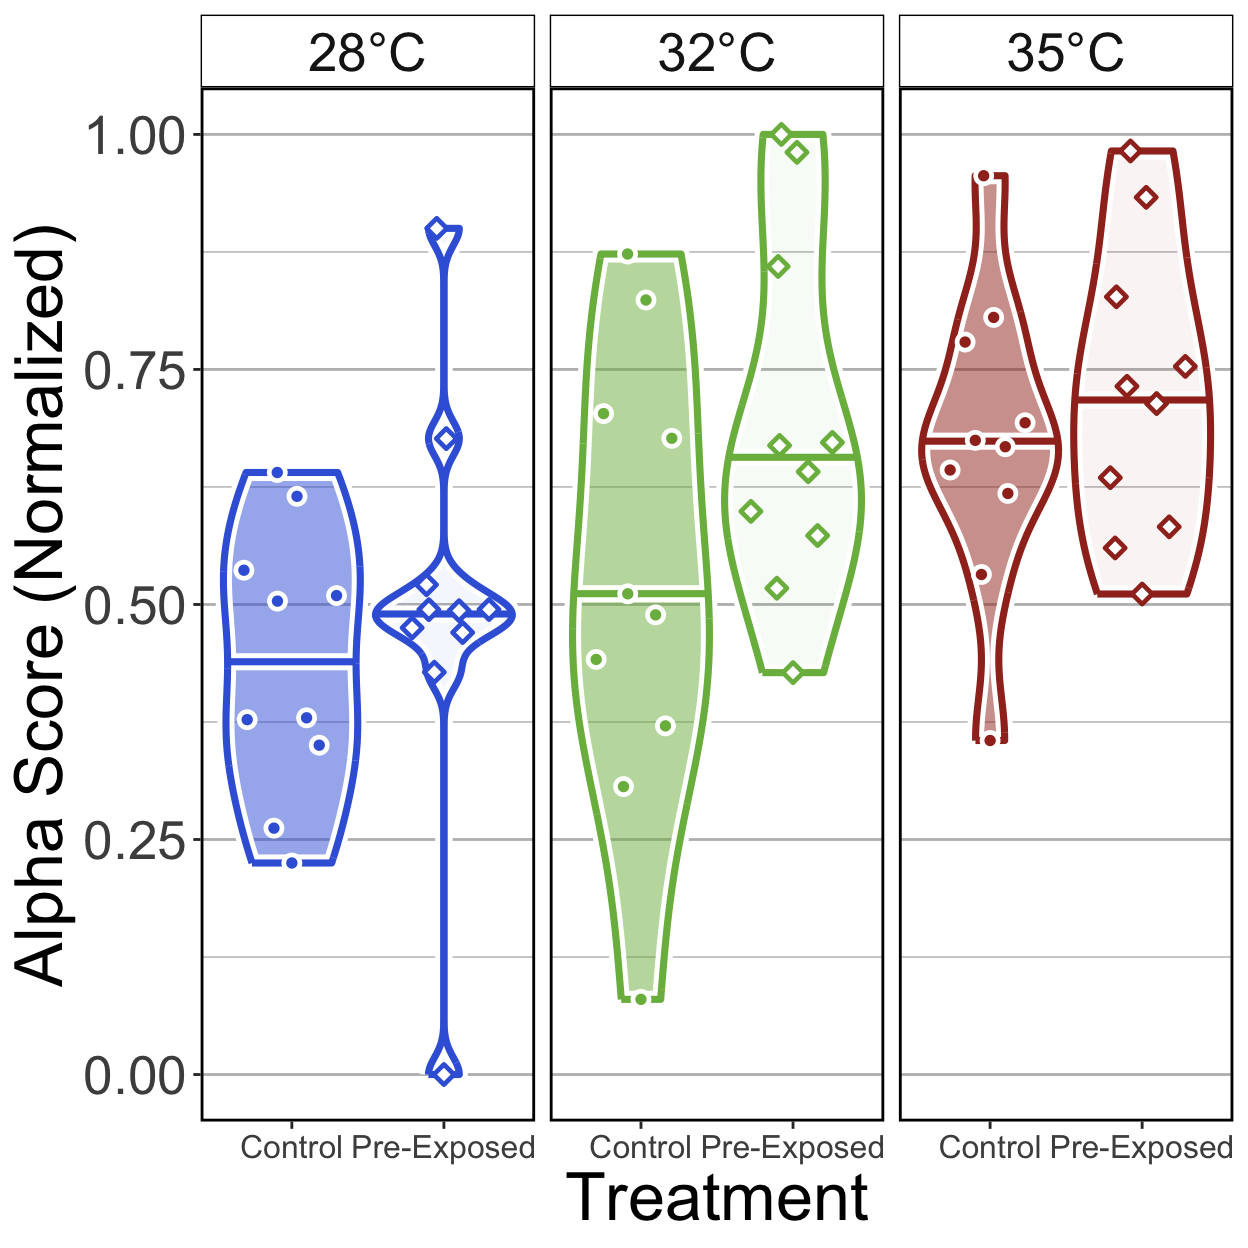
\includegraphics[keepaspectratio]{Results_Overview_files/figure-latex/plots-6A-1.pdf}}

\subparagraph{Tables}\label{tables-15}

(hide)

Click on tabs to display tables. Scroll to see additional rows.

GLM

\begin{longtable}{lrrrrl}
\caption*{
{\large GLM Results} \\ 
{\small glm(Alpha.Score \textasciitilde{} Temperature*Treatment); Pre-Exposed fish}
} \\ 
\toprule
term & estimate & std.error & statistic & p.value & p.adj.sig \\ 
\midrule\addlinespace[2.5pt]
\multicolumn{6}{l}{Shannon} \\ 
\midrule\addlinespace[2.5pt]
(Intercept) & $-0.218$ & $0.269$ & $-0.811$ & $\geq$0.25 & ns \\ 
Temperature32 & $0.345$ & $0.379$ & $0.910$ & $\geq$0.25 & ns \\ 
Temperature35 & $0.693$ & $0.384$ & $1.803$ & $0.077$ & ns \\ 
TreatmentExposed & $0.274$ & $0.379$ & $0.723$ & $\geq$0.25 & ns \\ 
Temperature32:TreatmentExposed & $0.311$ & $0.544$ & $0.572$ & $\geq$0.25 & ns \\ 
Temperature35:TreatmentExposed & $0.041$ & $0.550$ & $0.075$ & $\geq$0.25 & ns \\ 
\midrule\addlinespace[2.5pt]
\multicolumn{6}{l}{Simpson} \\ 
\midrule\addlinespace[2.5pt]
(Intercept) & $-0.241$ & $0.252$ & $-0.958$ & $\geq$0.25 & ns \\ 
Temperature32 & $0.352$ & $0.355$ & $0.990$ & $\geq$0.25 & ns \\ 
Temperature35 & $0.961$ & $0.367$ & $2.619$ & $0.011$ & * \\ 
TreatmentExposed & $0.223$ & $0.355$ & $0.627$ & $\geq$0.25 & ns \\ 
Temperature32:TreatmentExposed & $0.486$ & $0.513$ & $0.948$ & $\geq$0.25 & ns \\ 
Temperature35:TreatmentExposed & $0.017$ & $0.525$ & $0.033$ & $\geq$0.25 & ns \\ 
\midrule\addlinespace[2.5pt]
\multicolumn{6}{l}{Richness} \\ 
\midrule\addlinespace[2.5pt]
(Intercept) & $-0.145$ & $0.270$ & $-0.538$ & $\geq$0.25 & ns \\ 
Temperature32 & $0.550$ & $0.385$ & $1.430$ & $0.158$ & ns \\ 
Temperature35 & $0.043$ & $0.381$ & $0.112$ & $\geq$0.25 & ns \\ 
TreatmentExposed & $0.402$ & $0.382$ & $1.050$ & $\geq$0.25 & ns \\ 
Temperature32:TreatmentExposed & $0.020$ & $0.554$ & $0.036$ & $\geq$0.25 & ns \\ 
Temperature35:TreatmentExposed & $0.287$ & $0.545$ & $0.526$ & $\geq$0.25 & ns \\ 
\midrule\addlinespace[2.5pt]
\multicolumn{6}{l}{Phylogenetic} \\ 
\midrule\addlinespace[2.5pt]
(Intercept) & $-0.253$ & $0.254$ & $-0.996$ & $\geq$0.25 & ns \\ 
Temperature32 & $0.553$ & $0.360$ & $1.536$ & $0.130$ & ns \\ 
Temperature35 & $0.171$ & $0.358$ & $0.478$ & $\geq$0.25 & ns \\ 
TreatmentExposed & $0.335$ & $0.358$ & $0.937$ & $\geq$0.25 & ns \\ 
Temperature32:TreatmentExposed & $-0.018$ & $0.512$ & $-0.035$ & $\geq$0.25 & ns \\ 
Temperature35:TreatmentExposed & $0.102$ & $0.507$ & $0.201$ & $\geq$0.25 & ns \\ 
\bottomrule
\end{longtable}

ANOVA

\begin{longtable}{lrrrl}
\caption*{
{\large ANOVA of GLM} \\ 
{\small ANOVA(GLM(Alpha.Score \textasciitilde{} Temperature*Treatment), type = 2); Pre-Exposed fish}
} \\ 
\toprule
term & statistic & df & p.value & sig \\ 
\midrule\addlinespace[2.5pt]
\multicolumn{5}{l}{Shannon} \\ 
\midrule\addlinespace[2.5pt]
Temperature & $7.264$ & $2.000$ & $0.026$ & * \\ 
Treatment & $3.044$ & $1.000$ & $0.081$ & ns \\ 
Temperature:Treatment & $0.380$ & $2.000$ & $\geq$0.25 & ns \\ 
\midrule\addlinespace[2.5pt]
\multicolumn{5}{l}{Simpson} \\ 
\midrule\addlinespace[2.5pt]
Temperature & $14.462$ & $2.000$ & <0.001 & *** \\ 
Treatment & $3.406$ & $1.000$ & $0.065$ & ns \\ 
Temperature:Treatment & $1.122$ & $2.000$ & $\geq$0.25 & ns \\ 
\midrule\addlinespace[2.5pt]
\multicolumn{5}{l}{Richness} \\ 
\midrule\addlinespace[2.5pt]
Temperature & $4.311$ & $2.000$ & $0.116$ & ns \\ 
Treatment & $5.067$ & $1.000$ & $0.024$ & * \\ 
Temperature:Treatment & $0.340$ & $2.000$ & $\geq$0.25 & ns \\ 
\midrule\addlinespace[2.5pt]
\multicolumn{5}{l}{Phylogenetic} \\ 
\midrule\addlinespace[2.5pt]
Temperature & $4.600$ & $2.000$ & $0.100$ & ns \\ 
Treatment & $3.056$ & $1.000$ & $0.080$ & ns \\ 
Temperature:Treatment & $0.064$ & $2.000$ & $\geq$0.25 & ns \\ 
\bottomrule
\end{longtable}

Tukey

\begin{longtable}{cllllrrrrlc}
\caption*{
{\large Pairwise Tukey's HSD, p.adj: Dunnett} \\ 
{\small Tukey(Alpha.Score \textasciitilde{} Temperature*Treatment); Pre-Exposed fish}
} \\ 
\toprule
Temperature & .y. & term & group1 & group2 & estimate & std.error & statistic & adj.p.value & Variable & Group \\ 
\midrule\addlinespace[2.5pt]
\multicolumn{11}{l}{Shannon} \\ 
\midrule\addlinespace[2.5pt]
28 & Alpha.Score & Treatment & Exposed & Control & $0.274$ & $0.364$ & $0.753$ & $\geq$0.25 & Treatment & 28 \\ 
32 & Alpha.Score & Treatment & Exposed & Control & $0.585$ & $0.451$ & $1.298$ & $0.194$ & Treatment & 32 \\ 
35 & Alpha.Score & Treatment & Exposed & Control & $0.315$ & $0.344$ & $0.917$ & $\geq$0.25 & Treatment & 35 \\ 
\midrule\addlinespace[2.5pt]
\multicolumn{11}{l}{Simpson} \\ 
\midrule\addlinespace[2.5pt]
28 & Alpha.Score & Treatment & Exposed & Control & $0.223$ & $0.337$ & $0.662$ & $\geq$0.25 & Treatment & 28 \\ 
32 & Alpha.Score & Treatment & Exposed & Control & $0.709$ & $0.426$ & $1.663$ & $0.096$ & Treatment & 32 \\ 
35 & Alpha.Score & Treatment & Exposed & Control & $0.240$ & $0.339$ & $0.708$ & $\geq$0.25 & Treatment & 35 \\ 
\midrule\addlinespace[2.5pt]
\multicolumn{11}{l}{Richness} \\ 
\midrule\addlinespace[2.5pt]
28 & Alpha.Score & Treatment & Exposed & Control & $0.402$ & $0.361$ & $1.112$ & $\geq$0.25 & Treatment & 28 \\ 
32 & Alpha.Score & Treatment & Exposed & Control & $0.422$ & $0.411$ & $1.027$ & $\geq$0.25 & Treatment & 32 \\ 
35 & Alpha.Score & Treatment & Exposed & Control & $0.689$ & $0.400$ & $1.721$ & $0.085$ & Treatment & 35 \\ 
\midrule\addlinespace[2.5pt]
\multicolumn{11}{l}{Phylogenetic} \\ 
\midrule\addlinespace[2.5pt]
28 & Alpha.Score & Treatment & Exposed & Control & $0.335$ & $0.344$ & $0.974$ & $\geq$0.25 & Treatment & 28 \\ 
32 & Alpha.Score & Treatment & Exposed & Control & $0.317$ & $0.348$ & $0.911$ & $\geq$0.25 & Treatment & 32 \\ 
35 & Alpha.Score & Treatment & Exposed & Control & $0.437$ & $0.389$ & $1.123$ & $\geq$0.25 & Treatment & 35 \\ 
\bottomrule
\end{longtable}

\subparagraph{Addl. Metrics}\label{addl.-metrics-12}

\paragraph{6B)}\label{b-4}

\pandocbounded{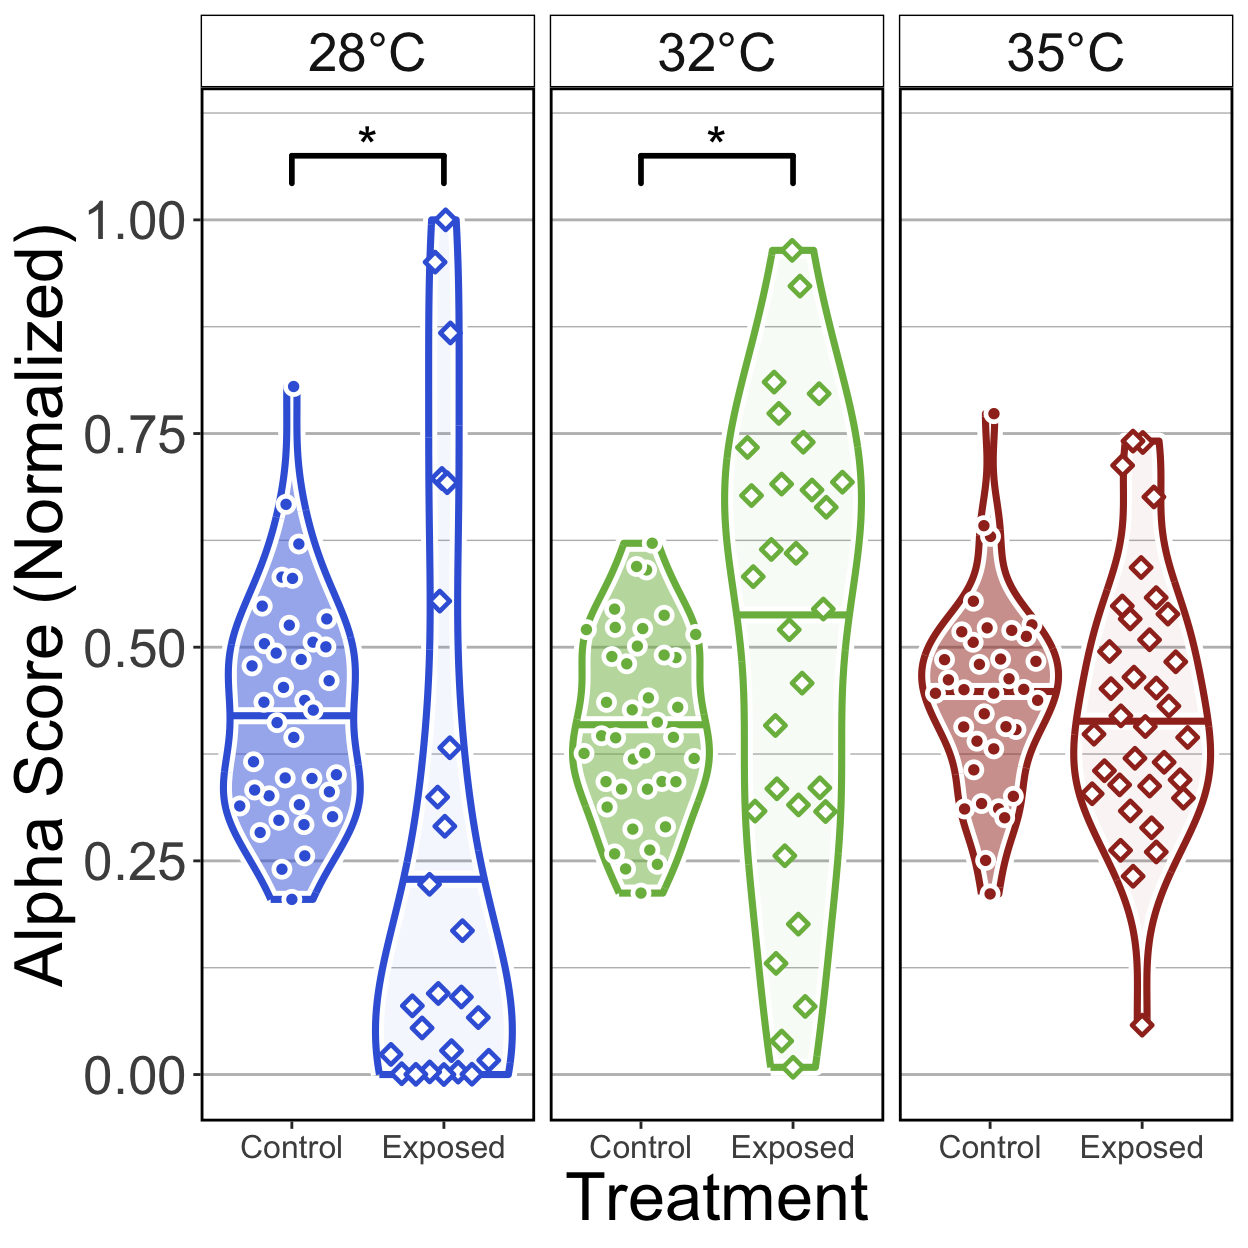
\includegraphics[keepaspectratio]{Results_Overview_files/figure-latex/plots-6B-1.pdf}}

\subparagraph{Tables}\label{tables-16}

(hide)

Click on tabs to display tables. Scroll to see additional rows.

GLM

\begin{longtable}{lrrrrl}
\caption*{
{\large GLM Results} \\ 
{\small glm(Alpha.Score \textasciitilde{} Temperature*Treatment); Post-Exposed fish}
} \\ 
\toprule
term & estimate & std.error & statistic & p.value & p.adj.sig \\ 
\midrule\addlinespace[2.5pt]
\multicolumn{6}{l}{Shannon} \\ 
\midrule\addlinespace[2.5pt]
(Intercept) & $-0.441$ & $0.126$ & $-3.499$ & <0.001 & *** \\ 
Temperature32 & $-0.064$ & $0.177$ & $-0.364$ & $\geq$0.25 & ns \\ 
Temperature35 & $-0.087$ & $0.182$ & $-0.476$ & $\geq$0.25 & ns \\ 
TreatmentExposed & $-0.539$ & $0.210$ & $-2.562$ & $0.011$ & * \\ 
Temperature32:TreatmentExposed & $0.953$ & $0.280$ & $3.405$ & <0.001 & *** \\ 
Temperature35:TreatmentExposed & $0.561$ & $0.281$ & $1.996$ & $0.047$ & * \\ 
\midrule\addlinespace[2.5pt]
\multicolumn{6}{l}{Simpson} \\ 
\midrule\addlinespace[2.5pt]
(Intercept) & $-0.299$ & $0.133$ & $-2.252$ & $0.025$ & * \\ 
Temperature32 & $-0.059$ & $0.186$ & $-0.319$ & $\geq$0.25 & ns \\ 
Temperature35 & $0.080$ & $0.190$ & $0.419$ & $\geq$0.25 & ns \\ 
TreatmentExposed & $-0.724$ & $0.225$ & $-3.223$ & $0.001$ & ** \\ 
Temperature32:TreatmentExposed & $1.106$ & $0.298$ & $3.715$ & <0.001 & *** \\ 
Temperature35:TreatmentExposed & $0.673$ & $0.297$ & $2.270$ & $0.024$ & * \\ 
\midrule\addlinespace[2.5pt]
\multicolumn{6}{l}{Richness} \\ 
\midrule\addlinespace[2.5pt]
(Intercept) & $-0.206$ & $0.101$ & $-2.040$ & $0.043$ & * \\ 
Temperature32 & $-0.048$ & $0.141$ & $-0.343$ & $\geq$0.25 & ns \\ 
Temperature35 & $-0.317$ & $0.147$ & $-2.164$ & $0.032$ & * \\ 
TreatmentExposed & $-0.228$ & $0.160$ & $-1.421$ & $0.157$ & ns \\ 
Temperature32:TreatmentExposed & $0.829$ & $0.219$ & $3.776$ & <0.001 & *** \\ 
Temperature35:TreatmentExposed & $0.691$ & $0.219$ & $3.155$ & $0.002$ & ** \\ 
\midrule\addlinespace[2.5pt]
\multicolumn{6}{l}{Phylogenetic} \\ 
\midrule\addlinespace[2.5pt]
(Intercept) & $-0.143$ & $0.095$ & $-1.507$ & $0.134$ & ns \\ 
Temperature32 & $-0.035$ & $0.132$ & $-0.268$ & $\geq$0.25 & ns \\ 
Temperature35 & $-0.319$ & $0.138$ & $-2.320$ & $0.021$ & * \\ 
TreatmentExposed & $-0.192$ & $0.150$ & $-1.280$ & $0.202$ & ns \\ 
Temperature32:TreatmentExposed & $0.780$ & $0.206$ & $3.783$ & <0.001 & *** \\ 
Temperature35:TreatmentExposed & $0.639$ & $0.205$ & $3.111$ & $0.002$ & ** \\ 
\bottomrule
\end{longtable}

ANOVA

\begin{longtable}{lrrrl}
\caption*{
{\large ANOVA of GLM} \\ 
{\small ANOVA(GLM(Alpha.Score \textasciitilde{} Temperature*Treatment), type = 2); Post-Exposed fish}
} \\ 
\toprule
term & statistic & df & p.value & sig \\ 
\midrule\addlinespace[2.5pt]
\multicolumn{5}{l}{Shannon} \\ 
\midrule\addlinespace[2.5pt]
Temperature & $5.908$ & $2.000$ & $0.052$ & ns \\ 
Treatment & $0.001$ & $1.000$ & $\geq$0.25 & ns \\ 
Temperature:Treatment & $11.784$ & $2.000$ & $0.003$ & ** \\ 
\midrule\addlinespace[2.5pt]
\multicolumn{5}{l}{Simpson} \\ 
\midrule\addlinespace[2.5pt]
Temperature & $8.400$ & $2.000$ & $0.015$ & * \\ 
Treatment & $0.547$ & $1.000$ & $\geq$0.25 & ns \\ 
Temperature:Treatment & $14.128$ & $2.000$ & <0.001 & *** \\ 
\midrule\addlinespace[2.5pt]
\multicolumn{5}{l}{Richness} \\ 
\midrule\addlinespace[2.5pt]
Temperature & $11.325$ & $2.000$ & $0.003$ & ** \\ 
Treatment & $11.824$ & $1.000$ & <0.001 & *** \\ 
Temperature:Treatment & $16.178$ & $2.000$ & <0.001 & *** \\ 
\midrule\addlinespace[2.5pt]
\multicolumn{5}{l}{Phylogenetic} \\ 
\midrule\addlinespace[2.5pt]
Temperature & $13.345$ & $2.000$ & $0.001$ & ** \\ 
Treatment & $13.294$ & $1.000$ & <0.001 & *** \\ 
Temperature:Treatment & $16.080$ & $2.000$ & <0.001 & *** \\ 
\bottomrule
\end{longtable}

Tukey

\begin{longtable}{cllllrrrrlc}
\caption*{
{\large Pairwise Tukey's HSD, p.adj: Dunnett} \\ 
{\small Tukey(Alpha.Score \textasciitilde{} Temperature*Treatment); Post-Exposed fish}
} \\ 
\toprule
Temperature & .y. & term & group1 & group2 & estimate & std.error & statistic & adj.p.value & Variable & Group \\ 
\midrule\addlinespace[2.5pt]
\multicolumn{11}{l}{Shannon} \\ 
\midrule\addlinespace[2.5pt]
28 & Alpha.Score & Treatment & Exposed & Control & $-0.539$ & $0.280$ & $-1.924$ & $0.054$ & Treatment & 28 \\ 
32 & Alpha.Score & Treatment & Exposed & Control & $0.414$ & $0.180$ & $2.298$ & $0.022$ & Treatment & 32 \\ 
35 & Alpha.Score & Treatment & Exposed & Control & $0.022$ & $0.111$ & $0.200$ & $\geq$0.25 & Treatment & 35 \\ 
\midrule\addlinespace[2.5pt]
\multicolumn{11}{l}{Simpson} \\ 
\midrule\addlinespace[2.5pt]
28 & Alpha.Score & Treatment & Exposed & Control & $-0.724$ & $0.290$ & $-2.492$ & $0.013$ & Treatment & 28 \\ 
32 & Alpha.Score & Treatment & Exposed & Control & $0.382$ & $0.190$ & $2.013$ & $0.044$ & Treatment & 32 \\ 
35 & Alpha.Score & Treatment & Exposed & Control & $-0.051$ & $0.130$ & $-0.387$ & $\geq$0.25 & Treatment & 35 \\ 
\midrule\addlinespace[2.5pt]
\multicolumn{11}{l}{Richness} \\ 
\midrule\addlinespace[2.5pt]
28 & Alpha.Score & Treatment & Exposed & Control & $-0.228$ & $0.223$ & $-1.021$ & $\geq$0.25 & Treatment & 28 \\ 
32 & Alpha.Score & Treatment & Exposed & Control & $0.601$ & $0.132$ & $4.546$ & <0.001 & Treatment & 32 \\ 
35 & Alpha.Score & Treatment & Exposed & Control & $0.463$ & $0.092$ & $5.021$ & <0.001 & Treatment & 35 \\ 
\midrule\addlinespace[2.5pt]
\multicolumn{11}{l}{Phylogenetic} \\ 
\midrule\addlinespace[2.5pt]
28 & Alpha.Score & Treatment & Exposed & Control & $-0.192$ & $0.210$ & $-0.916$ & $\geq$0.25 & Treatment & 28 \\ 
32 & Alpha.Score & Treatment & Exposed & Control & $0.588$ & $0.121$ & $4.858$ & <0.001 & Treatment & 32 \\ 
35 & Alpha.Score & Treatment & Exposed & Control & $0.447$ & $0.090$ & $4.961$ & <0.001 & Treatment & 35 \\ 
\bottomrule
\end{longtable}

\subparagraph{Addl. Metrics}\label{addl.-metrics-13}

\paragraph{6C)}\label{c-3}

\pandocbounded{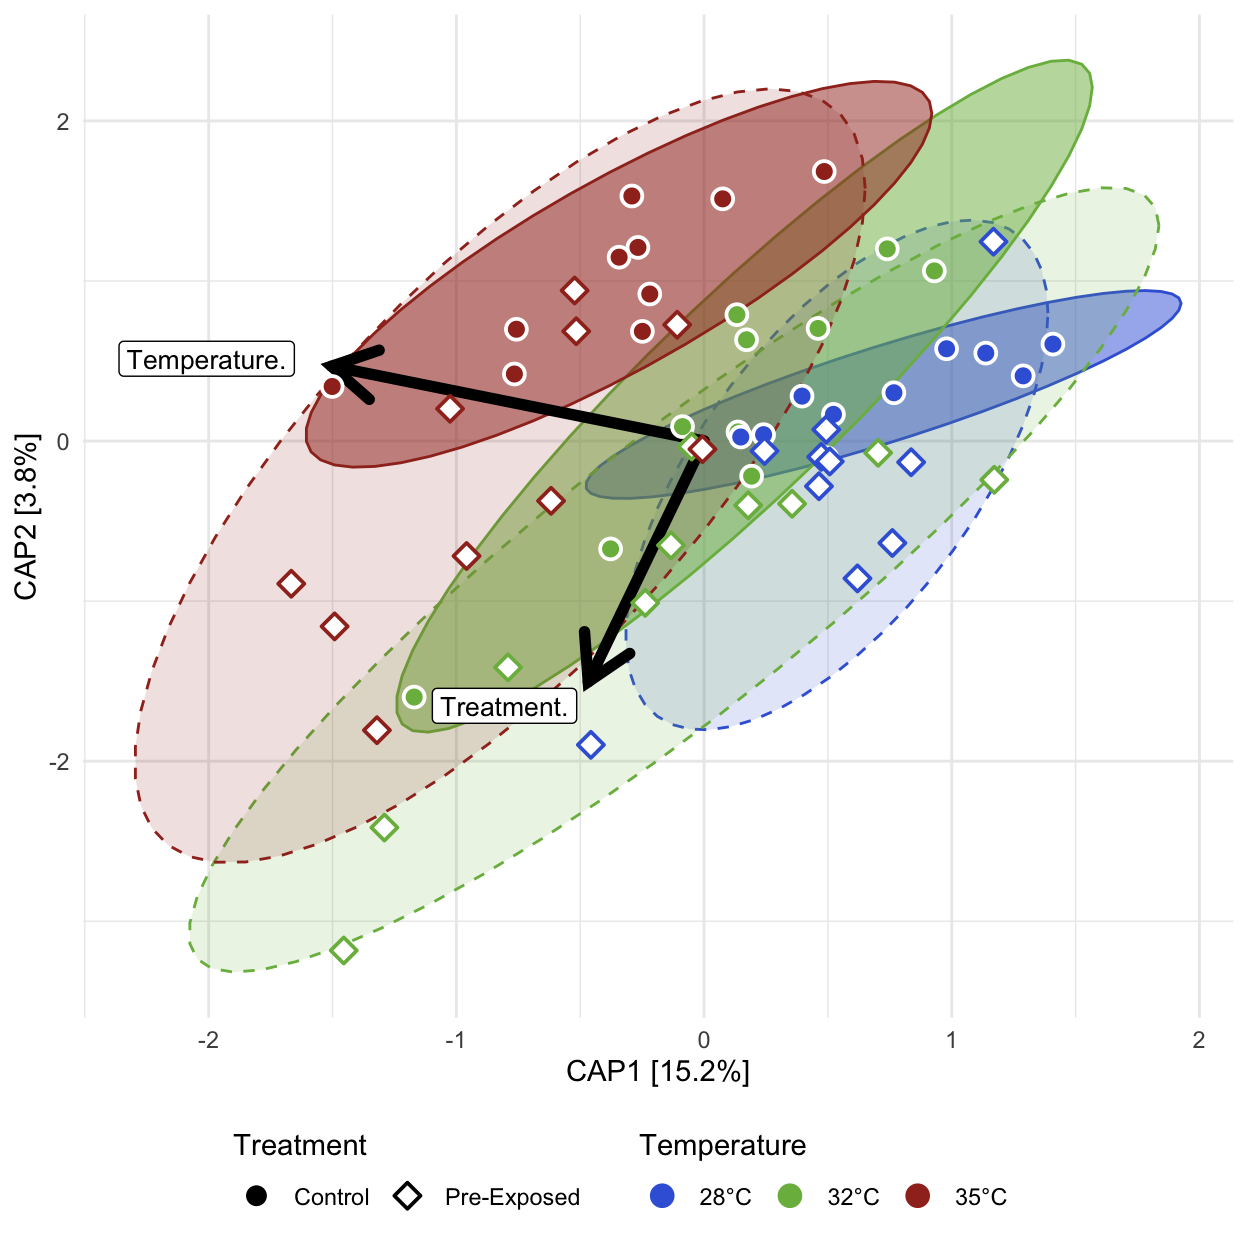
\includegraphics[keepaspectratio]{Results_Overview_files/figure-latex/plots-6C-1.pdf}}

\subparagraph{Tables}\label{tables-17}

(hide)

Click on tabs to display tables. Scroll to see additional rows.

ADONIS2

\begin{longtable}{lrrrrrl}
\caption*{
{\large ADONIS2} \\ 
{\small adonis2(Beta Distance \textasciitilde{} Temperature*Treatment); Pre-Exposed fish}
} \\ 
\toprule
term & df & SumOfSqs & R2 & statistic & p.value & sig \\ 
\midrule\addlinespace[2.5pt]
\multicolumn{7}{l}{bray} \\ 
\midrule\addlinespace[2.5pt]
Temperature & $2.000$ & $0.871$ & $0.188$ & $7.178$ & $0.001$ & *** \\ 
Treatment & $1.000$ & $0.244$ & $0.053$ & $4.025$ & $0.009$ & ** \\ 
Temperature:Treatment & $2.000$ & $0.245$ & $0.053$ & $2.019$ & $0.047$ & * \\ 
Residual & $54.000$ & $3.275$ & $0.707$ & NA & NA & NA \\ 
Total & $59.000$ & $4.635$ & $1.000$ & NA & NA & NA \\ 
\midrule\addlinespace[2.5pt]
\multicolumn{7}{l}{canberra} \\ 
\midrule\addlinespace[2.5pt]
Temperature & $2.000$ & $1.652$ & $0.132$ & $4.615$ & $0.001$ & *** \\ 
Treatment & $1.000$ & $0.533$ & $0.043$ & $2.979$ & $0.001$ & *** \\ 
Temperature:Treatment & $2.000$ & $0.667$ & $0.053$ & $1.864$ & $0.001$ & *** \\ 
Residual & $54.000$ & $9.665$ & $0.772$ & NA & NA & NA \\ 
Total & $59.000$ & $12.517$ & $1.000$ & NA & NA & NA \\ 
\midrule\addlinespace[2.5pt]
\multicolumn{7}{l}{gunifrac} \\ 
\midrule\addlinespace[2.5pt]
Temperature & $2.000$ & $0.647$ & $0.153$ & $5.604$ & $0.001$ & *** \\ 
Treatment & $1.000$ & $0.288$ & $0.068$ & $4.987$ & $0.003$ & ** \\ 
Temperature:Treatment & $2.000$ & $0.177$ & $0.042$ & $1.537$ & $0.110$ & ns \\ 
Residual & $54.000$ & $3.117$ & $0.737$ & NA & NA & NA \\ 
Total & $59.000$ & $4.229$ & $1.000$ & NA & NA & NA \\ 
\bottomrule
\end{longtable}

Dispersion (ANOVA)

\begin{longtable}{lrrrrrl}
\caption*{
{\large ANOVA: Homogeneity of Dispersion} \\ 
{\small ANOVA(Beta Disperson \textasciitilde{} Temperature); Pre-Exposed fish}
} \\ 
\toprule
term & df & sumsq & meansq & statistic & p.value & sig \\ 
\midrule\addlinespace[2.5pt]
\multicolumn{7}{l}{bray} \\ 
\midrule\addlinespace[2.5pt]
Temp.Treat & $5.000$ & $0.103$ & $0.021$ & $2.738$ & $0.028$ & * \\ 
Residual & $54.000$ & $0.405$ & $0.007$ & NA & NA & NA \\ 
\midrule\addlinespace[2.5pt]
\multicolumn{7}{l}{canberra} \\ 
\midrule\addlinespace[2.5pt]
Temp.Treat & $5.000$ & $0.014$ & $0.003$ & $0.453$ & $\geq$0.25 & ns \\ 
Residual & $54.000$ & $0.329$ & $0.006$ & NA & NA & NA \\ 
\midrule\addlinespace[2.5pt]
\multicolumn{7}{l}{gunifrac} \\ 
\midrule\addlinespace[2.5pt]
Temp.Treat & $5.000$ & $0.054$ & $0.011$ & $1.564$ & $0.186$ & ns \\ 
Residual & $54.000$ & $0.369$ & $0.007$ & NA & NA & NA \\ 
\bottomrule
\end{longtable}

Dispersion (Tukey)

\begin{longtable}{llllrrrrl}
\caption*{
{\large Tukey: Homogeneity of Dispersion} \\ 
{\small Tukey(Beta Disperson \textasciitilde{} Temperature*Treatment); Pre-Exposed fish}
} \\ 
\toprule
.y. & term & group1 & group2 & estimate & conf.low & conf.high & adj.p.value & sig \\ 
\midrule\addlinespace[2.5pt]
\multicolumn{9}{l}{bray} \\ 
\midrule\addlinespace[2.5pt]
Distance & Temp.Treat & 28°C\_\_Exposed & 28°C\_\_Control & $0.027$ & $-0.088$ & $0.141$ & $\geq$0.25 & ns \\ 
Distance & Temp.Treat & 32°C\_\_Control & 28°C\_\_Control & $0.095$ & $-0.019$ & $0.210$ & $0.153$ & ns \\ 
Distance & Temp.Treat & 32°C\_\_Exposed & 28°C\_\_Control & $0.110$ & $-0.004$ & $0.225$ & $0.065$ & ns \\ 
Distance & Temp.Treat & 35°C\_\_Control & 28°C\_\_Control & $0.015$ & $-0.099$ & $0.130$ & $\geq$0.25 & ns \\ 
Distance & Temp.Treat & 35°C\_\_Exposed & 28°C\_\_Control & $0.069$ & $-0.045$ & $0.183$ & $\geq$0.25 & ns \\ 
Distance & Temp.Treat & 32°C\_\_Control & 28°C\_\_Exposed & $0.069$ & $-0.046$ & $0.183$ & $\geq$0.25 & ns \\ 
Distance & Temp.Treat & 32°C\_\_Exposed & 28°C\_\_Exposed & $0.084$ & $-0.031$ & $0.198$ & $\geq$0.25 & ns \\ 
Distance & Temp.Treat & 35°C\_\_Control & 28°C\_\_Exposed & $-0.011$ & $-0.126$ & $0.103$ & $\geq$0.25 & ns \\ 
Distance & Temp.Treat & 35°C\_\_Exposed & 28°C\_\_Exposed & $0.042$ & $-0.072$ & $0.157$ & $\geq$0.25 & ns \\ 
Distance & Temp.Treat & 32°C\_\_Exposed & 32°C\_\_Control & $0.015$ & $-0.100$ & $0.129$ & $\geq$0.25 & ns \\ 
Distance & Temp.Treat & 35°C\_\_Control & 32°C\_\_Control & $-0.080$ & $-0.195$ & $0.034$ & $\geq$0.25 & ns \\ 
Distance & Temp.Treat & 35°C\_\_Exposed & 32°C\_\_Control & $-0.026$ & $-0.141$ & $0.088$ & $\geq$0.25 & ns \\ 
Distance & Temp.Treat & 35°C\_\_Control & 32°C\_\_Exposed & $-0.095$ & $-0.209$ & $0.019$ & $0.156$ & ns \\ 
Distance & Temp.Treat & 35°C\_\_Exposed & 32°C\_\_Exposed & $-0.041$ & $-0.156$ & $0.073$ & $\geq$0.25 & ns \\ 
Distance & Temp.Treat & 35°C\_\_Exposed & 35°C\_\_Control & $0.054$ & $-0.061$ & $0.168$ & $\geq$0.25 & ns \\ 
\midrule\addlinespace[2.5pt]
\multicolumn{9}{l}{canberra} \\ 
\midrule\addlinespace[2.5pt]
Distance & Temp.Treat & 28°C\_\_Exposed & 28°C\_\_Control & $0.011$ & $-0.092$ & $0.114$ & $\geq$0.25 & ns \\ 
Distance & Temp.Treat & 32°C\_\_Control & 28°C\_\_Control & $0.035$ & $-0.068$ & $0.138$ & $\geq$0.25 & ns \\ 
Distance & Temp.Treat & 32°C\_\_Exposed & 28°C\_\_Control & $0.044$ & $-0.059$ & $0.147$ & $\geq$0.25 & ns \\ 
Distance & Temp.Treat & 35°C\_\_Control & 28°C\_\_Control & $0.010$ & $-0.094$ & $0.113$ & $\geq$0.25 & ns \\ 
Distance & Temp.Treat & 35°C\_\_Exposed & 28°C\_\_Control & $0.016$ & $-0.087$ & $0.119$ & $\geq$0.25 & ns \\ 
Distance & Temp.Treat & 32°C\_\_Control & 28°C\_\_Exposed & $0.024$ & $-0.079$ & $0.127$ & $\geq$0.25 & ns \\ 
Distance & Temp.Treat & 32°C\_\_Exposed & 28°C\_\_Exposed & $0.033$ & $-0.070$ & $0.136$ & $\geq$0.25 & ns \\ 
Distance & Temp.Treat & 35°C\_\_Control & 28°C\_\_Exposed & $-0.001$ & $-0.104$ & $0.102$ & $\geq$0.25 & ns \\ 
Distance & Temp.Treat & 35°C\_\_Exposed & 28°C\_\_Exposed & $0.005$ & $-0.098$ & $0.108$ & $\geq$0.25 & ns \\ 
Distance & Temp.Treat & 32°C\_\_Exposed & 32°C\_\_Control & $0.009$ & $-0.094$ & $0.112$ & $\geq$0.25 & ns \\ 
Distance & Temp.Treat & 35°C\_\_Control & 32°C\_\_Control & $-0.025$ & $-0.128$ & $0.078$ & $\geq$0.25 & ns \\ 
Distance & Temp.Treat & 35°C\_\_Exposed & 32°C\_\_Control & $-0.019$ & $-0.122$ & $0.084$ & $\geq$0.25 & ns \\ 
Distance & Temp.Treat & 35°C\_\_Control & 32°C\_\_Exposed & $-0.034$ & $-0.137$ & $0.069$ & $\geq$0.25 & ns \\ 
Distance & Temp.Treat & 35°C\_\_Exposed & 32°C\_\_Exposed & $-0.028$ & $-0.131$ & $0.075$ & $\geq$0.25 & ns \\ 
Distance & Temp.Treat & 35°C\_\_Exposed & 35°C\_\_Control & $0.006$ & $-0.097$ & $0.109$ & $\geq$0.25 & ns \\ 
\midrule\addlinespace[2.5pt]
\multicolumn{9}{l}{gunifrac} \\ 
\midrule\addlinespace[2.5pt]
Distance & Temp.Treat & 28°C\_\_Exposed & 28°C\_\_Control & $0.003$ & $-0.106$ & $0.112$ & $\geq$0.25 & ns \\ 
Distance & Temp.Treat & 32°C\_\_Control & 28°C\_\_Control & $0.051$ & $-0.058$ & $0.160$ & $\geq$0.25 & ns \\ 
Distance & Temp.Treat & 32°C\_\_Exposed & 28°C\_\_Control & $0.078$ & $-0.032$ & $0.187$ & $\geq$0.25 & ns \\ 
Distance & Temp.Treat & 35°C\_\_Control & 28°C\_\_Control & $0.000$ & $-0.109$ & $0.110$ & $\geq$0.25 & ns \\ 
Distance & Temp.Treat & 35°C\_\_Exposed & 28°C\_\_Control & $0.042$ & $-0.067$ & $0.151$ & $\geq$0.25 & ns \\ 
Distance & Temp.Treat & 32°C\_\_Control & 28°C\_\_Exposed & $0.048$ & $-0.061$ & $0.158$ & $\geq$0.25 & ns \\ 
Distance & Temp.Treat & 32°C\_\_Exposed & 28°C\_\_Exposed & $0.075$ & $-0.035$ & $0.184$ & $\geq$0.25 & ns \\ 
Distance & Temp.Treat & 35°C\_\_Control & 28°C\_\_Exposed & $-0.002$ & $-0.112$ & $0.107$ & $\geq$0.25 & ns \\ 
Distance & Temp.Treat & 35°C\_\_Exposed & 28°C\_\_Exposed & $0.039$ & $-0.070$ & $0.148$ & $\geq$0.25 & ns \\ 
Distance & Temp.Treat & 32°C\_\_Exposed & 32°C\_\_Control & $0.026$ & $-0.083$ & $0.136$ & $\geq$0.25 & ns \\ 
Distance & Temp.Treat & 35°C\_\_Control & 32°C\_\_Control & $-0.051$ & $-0.160$ & $0.059$ & $\geq$0.25 & ns \\ 
Distance & Temp.Treat & 35°C\_\_Exposed & 32°C\_\_Control & $-0.009$ & $-0.118$ & $0.100$ & $\geq$0.25 & ns \\ 
Distance & Temp.Treat & 35°C\_\_Control & 32°C\_\_Exposed & $-0.077$ & $-0.186$ & $0.032$ & $\geq$0.25 & ns \\ 
Distance & Temp.Treat & 35°C\_\_Exposed & 32°C\_\_Exposed & $-0.036$ & $-0.145$ & $0.074$ & $\geq$0.25 & ns \\ 
Distance & Temp.Treat & 35°C\_\_Exposed & 35°C\_\_Control & $0.041$ & $-0.068$ & $0.151$ & $\geq$0.25 & ns \\ 
\bottomrule
\end{longtable}

\subparagraph{Addl. Metrics}\label{addl.-metrics-14}

\paragraph{6D)}\label{d-3}

\pandocbounded{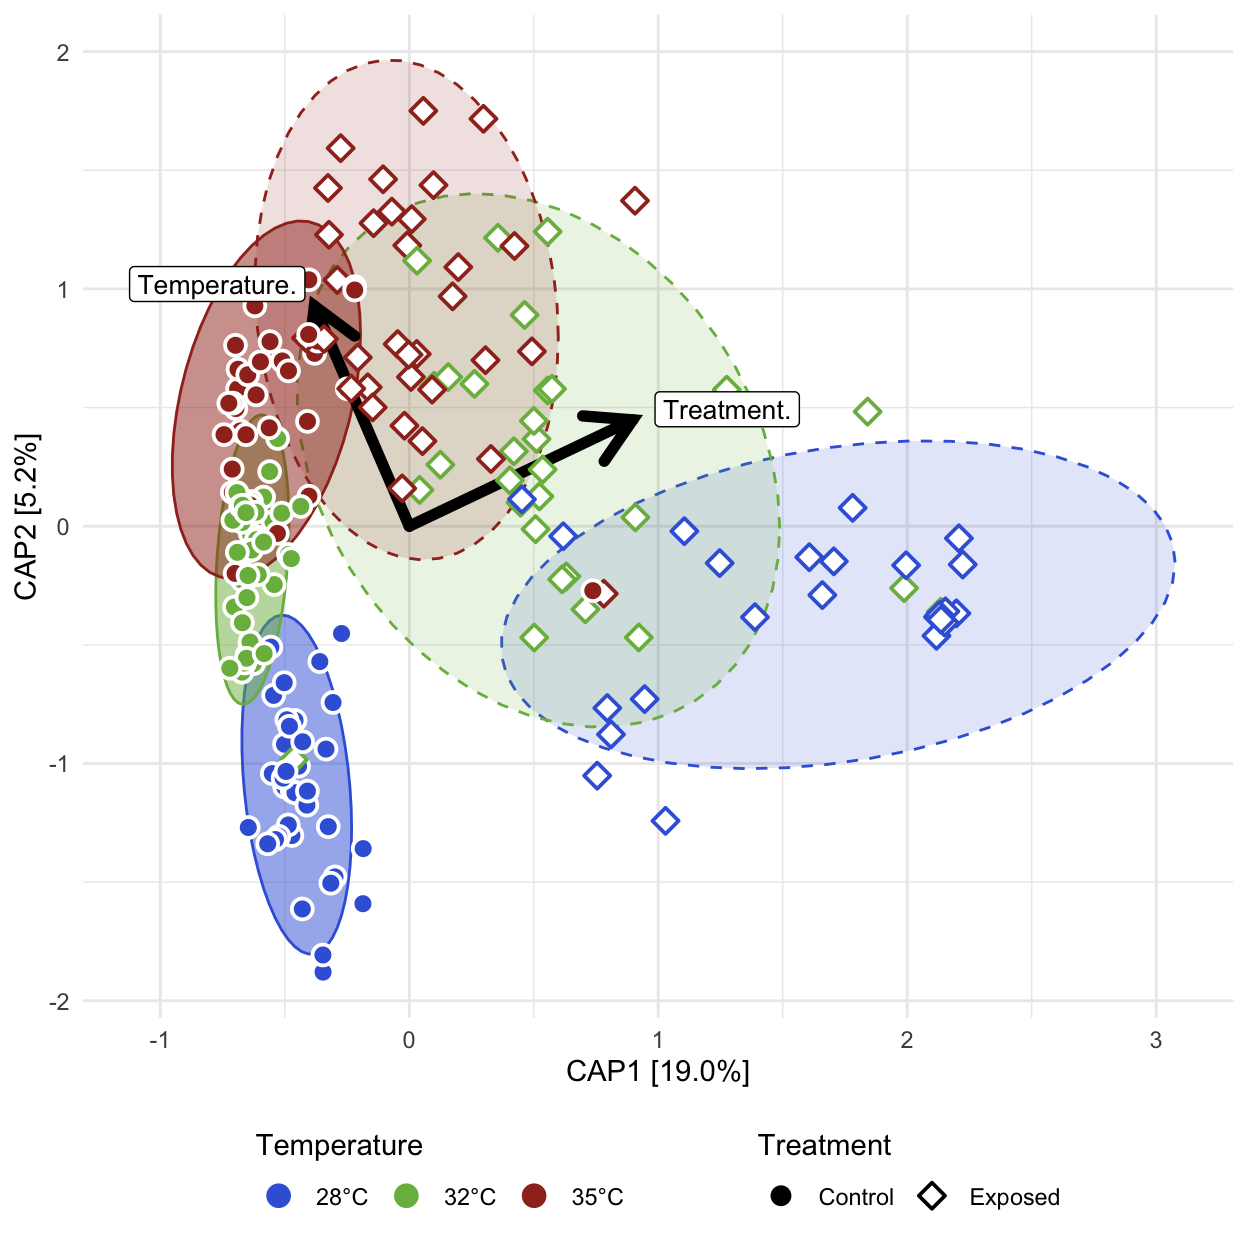
\includegraphics[keepaspectratio]{Results_Overview_files/figure-latex/plots-6D-1.pdf}}

\subparagraph{Tables}\label{tables-18}

(hide)

Click on tabs to display tables. Scroll to see additional rows.

ADONIS2

\begin{longtable}{lrrrrrr}
\caption*{
{\large ADONIS2} \\ 
{\small adonis2(Beta Distance \textasciitilde{} Temperature*Treatment); Post-Exposed fish}
} \\ 
\toprule
term & df & SumOfSqs & R2 & statistic & p.value & sig \\ 
\midrule\addlinespace[2.5pt]
\multicolumn{7}{l}{bray} \\ 
\midrule\addlinespace[2.5pt]
Temperature & $2.000$ & $4.123$ & $0.108$ & $17.035$ & $0.001$ & *** \\ 
Treatment & $1.000$ & $7.411$ & $0.194$ & $61.235$ & $0.001$ & *** \\ 
Temperature:Treatment & $2.000$ & $3.168$ & $0.083$ & $13.088$ & $0.001$ & *** \\ 
Residual & $194.000$ & $23.478$ & $0.615$ & NA & NA & NA \\ 
Total & $199.000$ & $38.179$ & $1.000$ & NA & NA & NA \\ 
\midrule\addlinespace[2.5pt]
\multicolumn{7}{l}{canberra} \\ 
\midrule\addlinespace[2.5pt]
Temperature & $2.000$ & $4.561$ & $0.074$ & $9.502$ & $0.001$ & *** \\ 
Treatment & $1.000$ & $7.402$ & $0.120$ & $30.840$ & $0.001$ & *** \\ 
Temperature:Treatment & $2.000$ & $3.014$ & $0.049$ & $6.279$ & $0.001$ & *** \\ 
Residual & $194.000$ & $46.561$ & $0.757$ & NA & NA & NA \\ 
Total & $199.000$ & $61.538$ & $1.000$ & NA & NA & NA \\ 
\midrule\addlinespace[2.5pt]
\multicolumn{7}{l}{gunifrac} \\ 
\midrule\addlinespace[2.5pt]
Temperature & $2.000$ & $2.273$ & $0.082$ & $11.945$ & $0.001$ & *** \\ 
Treatment & $1.000$ & $4.718$ & $0.170$ & $49.577$ & $0.001$ & *** \\ 
Temperature:Treatment & $2.000$ & $2.273$ & $0.082$ & $11.944$ & $0.001$ & *** \\ 
Residual & $194.000$ & $18.460$ & $0.666$ & NA & NA & NA \\ 
Total & $199.000$ & $27.724$ & $1.000$ & NA & NA & NA \\ 
\bottomrule
\end{longtable}

Dispersion (ANOVA)

\begin{longtable}{lrrrrrr}
\caption*{
{\large ANOVA: Homogeneity of Dispersion} \\ 
{\small ANOVA(Beta Disperson \textasciitilde{} Temperature); Post-Exposed fish}
} \\ 
\toprule
term & df & sumsq & meansq & statistic & p.value & sig \\ 
\midrule\addlinespace[2.5pt]
\multicolumn{7}{l}{bray} \\ 
\midrule\addlinespace[2.5pt]
Temp.Treat & $5.000$ & $1.344$ & $0.269$ & $17.882$ & <0.001 & **** \\ 
Residual & $194.000$ & $2.917$ & $0.015$ & NA & NA & NA \\ 
\midrule\addlinespace[2.5pt]
\multicolumn{7}{l}{canberra} \\ 
\midrule\addlinespace[2.5pt]
Temp.Treat & $5.000$ & $1.094$ & $0.219$ & $31.758$ & <0.001 & **** \\ 
Residual & $194.000$ & $1.337$ & $0.007$ & NA & NA & NA \\ 
\midrule\addlinespace[2.5pt]
\multicolumn{7}{l}{gunifrac} \\ 
\midrule\addlinespace[2.5pt]
Temp.Treat & $5.000$ & $1.225$ & $0.245$ & $29.264$ & <0.001 & **** \\ 
Residual & $194.000$ & $1.624$ & $0.008$ & NA & NA & NA \\ 
\bottomrule
\end{longtable}

Dispersion (Tukey)

\begin{longtable}{llllrrrrl}
\caption*{
{\large Tukey: Homogeneity of Dispersion} \\ 
{\small Tukey(Beta Disperson \textasciitilde{} Temperature*Treatment); Post-Exposed fish}
} \\ 
\toprule
.y. & term & group1 & group2 & estimate & conf.low & conf.high & adj.p.value & sig \\ 
\midrule\addlinespace[2.5pt]
\multicolumn{9}{l}{bray} \\ 
\midrule\addlinespace[2.5pt]
Distance & Temp.Treat & 28°C\_\_Exposed & 28°C\_\_Control & $0.211$ & $0.119$ & $0.302$ & <0.001 & **** \\ 
Distance & Temp.Treat & 32°C\_\_Control & 28°C\_\_Control & $-0.015$ & $-0.096$ & $0.066$ & $\geq$0.25 & ns \\ 
Distance & Temp.Treat & 32°C\_\_Exposed & 28°C\_\_Control & $0.168$ & $0.081$ & $0.255$ & <0.001 & **** \\ 
Distance & Temp.Treat & 35°C\_\_Control & 28°C\_\_Control & $0.013$ & $-0.070$ & $0.096$ & $\geq$0.25 & ns \\ 
Distance & Temp.Treat & 35°C\_\_Exposed & 28°C\_\_Control & $0.060$ & $-0.024$ & $0.144$ & $\geq$0.25 & ns \\ 
Distance & Temp.Treat & 32°C\_\_Control & 28°C\_\_Exposed & $-0.225$ & $-0.316$ & $-0.135$ & <0.001 & **** \\ 
Distance & Temp.Treat & 32°C\_\_Exposed & 28°C\_\_Exposed & $-0.043$ & $-0.138$ & $0.053$ & $\geq$0.25 & ns \\ 
Distance & Temp.Treat & 35°C\_\_Control & 28°C\_\_Exposed & $-0.197$ & $-0.290$ & $-0.105$ & <0.001 & **** \\ 
Distance & Temp.Treat & 35°C\_\_Exposed & 28°C\_\_Exposed & $-0.150$ & $-0.243$ & $-0.057$ & <0.001 & **** \\ 
Distance & Temp.Treat & 32°C\_\_Exposed & 32°C\_\_Control & $0.183$ & $0.097$ & $0.268$ & <0.001 & **** \\ 
Distance & Temp.Treat & 35°C\_\_Control & 32°C\_\_Control & $0.028$ & $-0.054$ & $0.110$ & $\geq$0.25 & ns \\ 
Distance & Temp.Treat & 35°C\_\_Exposed & 32°C\_\_Control & $0.075$ & $-0.008$ & $0.158$ & $0.100$ & ns \\ 
Distance & Temp.Treat & 35°C\_\_Control & 32°C\_\_Exposed & $-0.155$ & $-0.243$ & $-0.067$ & <0.001 & **** \\ 
Distance & Temp.Treat & 35°C\_\_Exposed & 32°C\_\_Exposed & $-0.108$ & $-0.196$ & $-0.019$ & $0.007$ & ** \\ 
Distance & Temp.Treat & 35°C\_\_Exposed & 35°C\_\_Control & $0.047$ & $-0.038$ & $0.132$ & $\geq$0.25 & ns \\ 
\midrule\addlinespace[2.5pt]
\multicolumn{9}{l}{canberra} \\ 
\midrule\addlinespace[2.5pt]
Distance & Temp.Treat & 28°C\_\_Exposed & 28°C\_\_Control & $0.217$ & $0.155$ & $0.279$ & <0.001 & **** \\ 
Distance & Temp.Treat & 32°C\_\_Control & 28°C\_\_Control & $-0.011$ & $-0.066$ & $0.044$ & $\geq$0.25 & ns \\ 
Distance & Temp.Treat & 32°C\_\_Exposed & 28°C\_\_Control & $0.107$ & $0.048$ & $0.166$ & <0.001 & **** \\ 
Distance & Temp.Treat & 35°C\_\_Control & 28°C\_\_Control & $0.013$ & $-0.044$ & $0.069$ & $\geq$0.25 & ns \\ 
Distance & Temp.Treat & 35°C\_\_Exposed & 28°C\_\_Control & $0.073$ & $0.016$ & $0.130$ & $0.004$ & ** \\ 
Distance & Temp.Treat & 32°C\_\_Control & 28°C\_\_Exposed & $-0.228$ & $-0.289$ & $-0.167$ & <0.001 & **** \\ 
Distance & Temp.Treat & 32°C\_\_Exposed & 28°C\_\_Exposed & $-0.110$ & $-0.175$ & $-0.045$ & <0.001 & **** \\ 
Distance & Temp.Treat & 35°C\_\_Control & 28°C\_\_Exposed & $-0.204$ & $-0.267$ & $-0.142$ & <0.001 & **** \\ 
Distance & Temp.Treat & 35°C\_\_Exposed & 28°C\_\_Exposed & $-0.144$ & $-0.207$ & $-0.081$ & <0.001 & **** \\ 
Distance & Temp.Treat & 32°C\_\_Exposed & 32°C\_\_Control & $0.118$ & $0.060$ & $0.176$ & <0.001 & **** \\ 
Distance & Temp.Treat & 35°C\_\_Control & 32°C\_\_Control & $0.024$ & $-0.032$ & $0.080$ & $\geq$0.25 & ns \\ 
Distance & Temp.Treat & 35°C\_\_Exposed & 32°C\_\_Control & $0.084$ & $0.028$ & $0.140$ & <0.001 & *** \\ 
Distance & Temp.Treat & 35°C\_\_Control & 32°C\_\_Exposed & $-0.094$ & $-0.154$ & $-0.035$ & <0.001 & *** \\ 
Distance & Temp.Treat & 35°C\_\_Exposed & 32°C\_\_Exposed & $-0.034$ & $-0.094$ & $0.026$ & $\geq$0.25 & ns \\ 
Distance & Temp.Treat & 35°C\_\_Exposed & 35°C\_\_Control & $0.060$ & $0.003$ & $0.118$ & $0.035$ & * \\ 
\midrule\addlinespace[2.5pt]
\multicolumn{9}{l}{gunifrac} \\ 
\midrule\addlinespace[2.5pt]
Distance & Temp.Treat & 28°C\_\_Exposed & 28°C\_\_Control & $0.197$ & $0.129$ & $0.266$ & <0.001 & **** \\ 
Distance & Temp.Treat & 32°C\_\_Control & 28°C\_\_Control & $-0.023$ & $-0.083$ & $0.037$ & $\geq$0.25 & ns \\ 
Distance & Temp.Treat & 32°C\_\_Exposed & 28°C\_\_Control & $0.141$ & $0.077$ & $0.206$ & <0.001 & **** \\ 
Distance & Temp.Treat & 35°C\_\_Control & 28°C\_\_Control & $-0.011$ & $-0.073$ & $0.051$ & $\geq$0.25 & ns \\ 
Distance & Temp.Treat & 35°C\_\_Exposed & 28°C\_\_Control & $0.054$ & $-0.009$ & $0.117$ & $0.134$ & ns \\ 
Distance & Temp.Treat & 32°C\_\_Control & 28°C\_\_Exposed & $-0.220$ & $-0.288$ & $-0.153$ & <0.001 & **** \\ 
Distance & Temp.Treat & 32°C\_\_Exposed & 28°C\_\_Exposed & $-0.056$ & $-0.128$ & $0.015$ & $0.211$ & ns \\ 
Distance & Temp.Treat & 35°C\_\_Control & 28°C\_\_Exposed & $-0.209$ & $-0.278$ & $-0.140$ & <0.001 & **** \\ 
Distance & Temp.Treat & 35°C\_\_Exposed & 28°C\_\_Exposed & $-0.143$ & $-0.213$ & $-0.074$ & <0.001 & **** \\ 
Distance & Temp.Treat & 32°C\_\_Exposed & 32°C\_\_Control & $0.164$ & $0.100$ & $0.228$ & <0.001 & **** \\ 
Distance & Temp.Treat & 35°C\_\_Control & 32°C\_\_Control & $0.012$ & $-0.050$ & $0.073$ & $\geq$0.25 & ns \\ 
Distance & Temp.Treat & 35°C\_\_Exposed & 32°C\_\_Control & $0.077$ & $0.015$ & $0.139$ & $0.006$ & ** \\ 
Distance & Temp.Treat & 35°C\_\_Control & 32°C\_\_Exposed & $-0.152$ & $-0.218$ & $-0.087$ & <0.001 & **** \\ 
Distance & Temp.Treat & 35°C\_\_Exposed & 32°C\_\_Exposed & $-0.087$ & $-0.153$ & $-0.021$ & $0.003$ & ** \\ 
Distance & Temp.Treat & 35°C\_\_Exposed & 35°C\_\_Control & $0.065$ & $0.002$ & $0.129$ & $0.039$ & * \\ 
\bottomrule
\end{longtable}

\subparagraph{Addl. Metrics}\label{addl.-metrics-15}

\subsubsection{}\label{section-5}

\paragraph{(hide)}\label{hide-24}

Click on tabs to reveal figures displaying additional metrics.

\paragraph{S6A}\label{s6a}

\pandocbounded{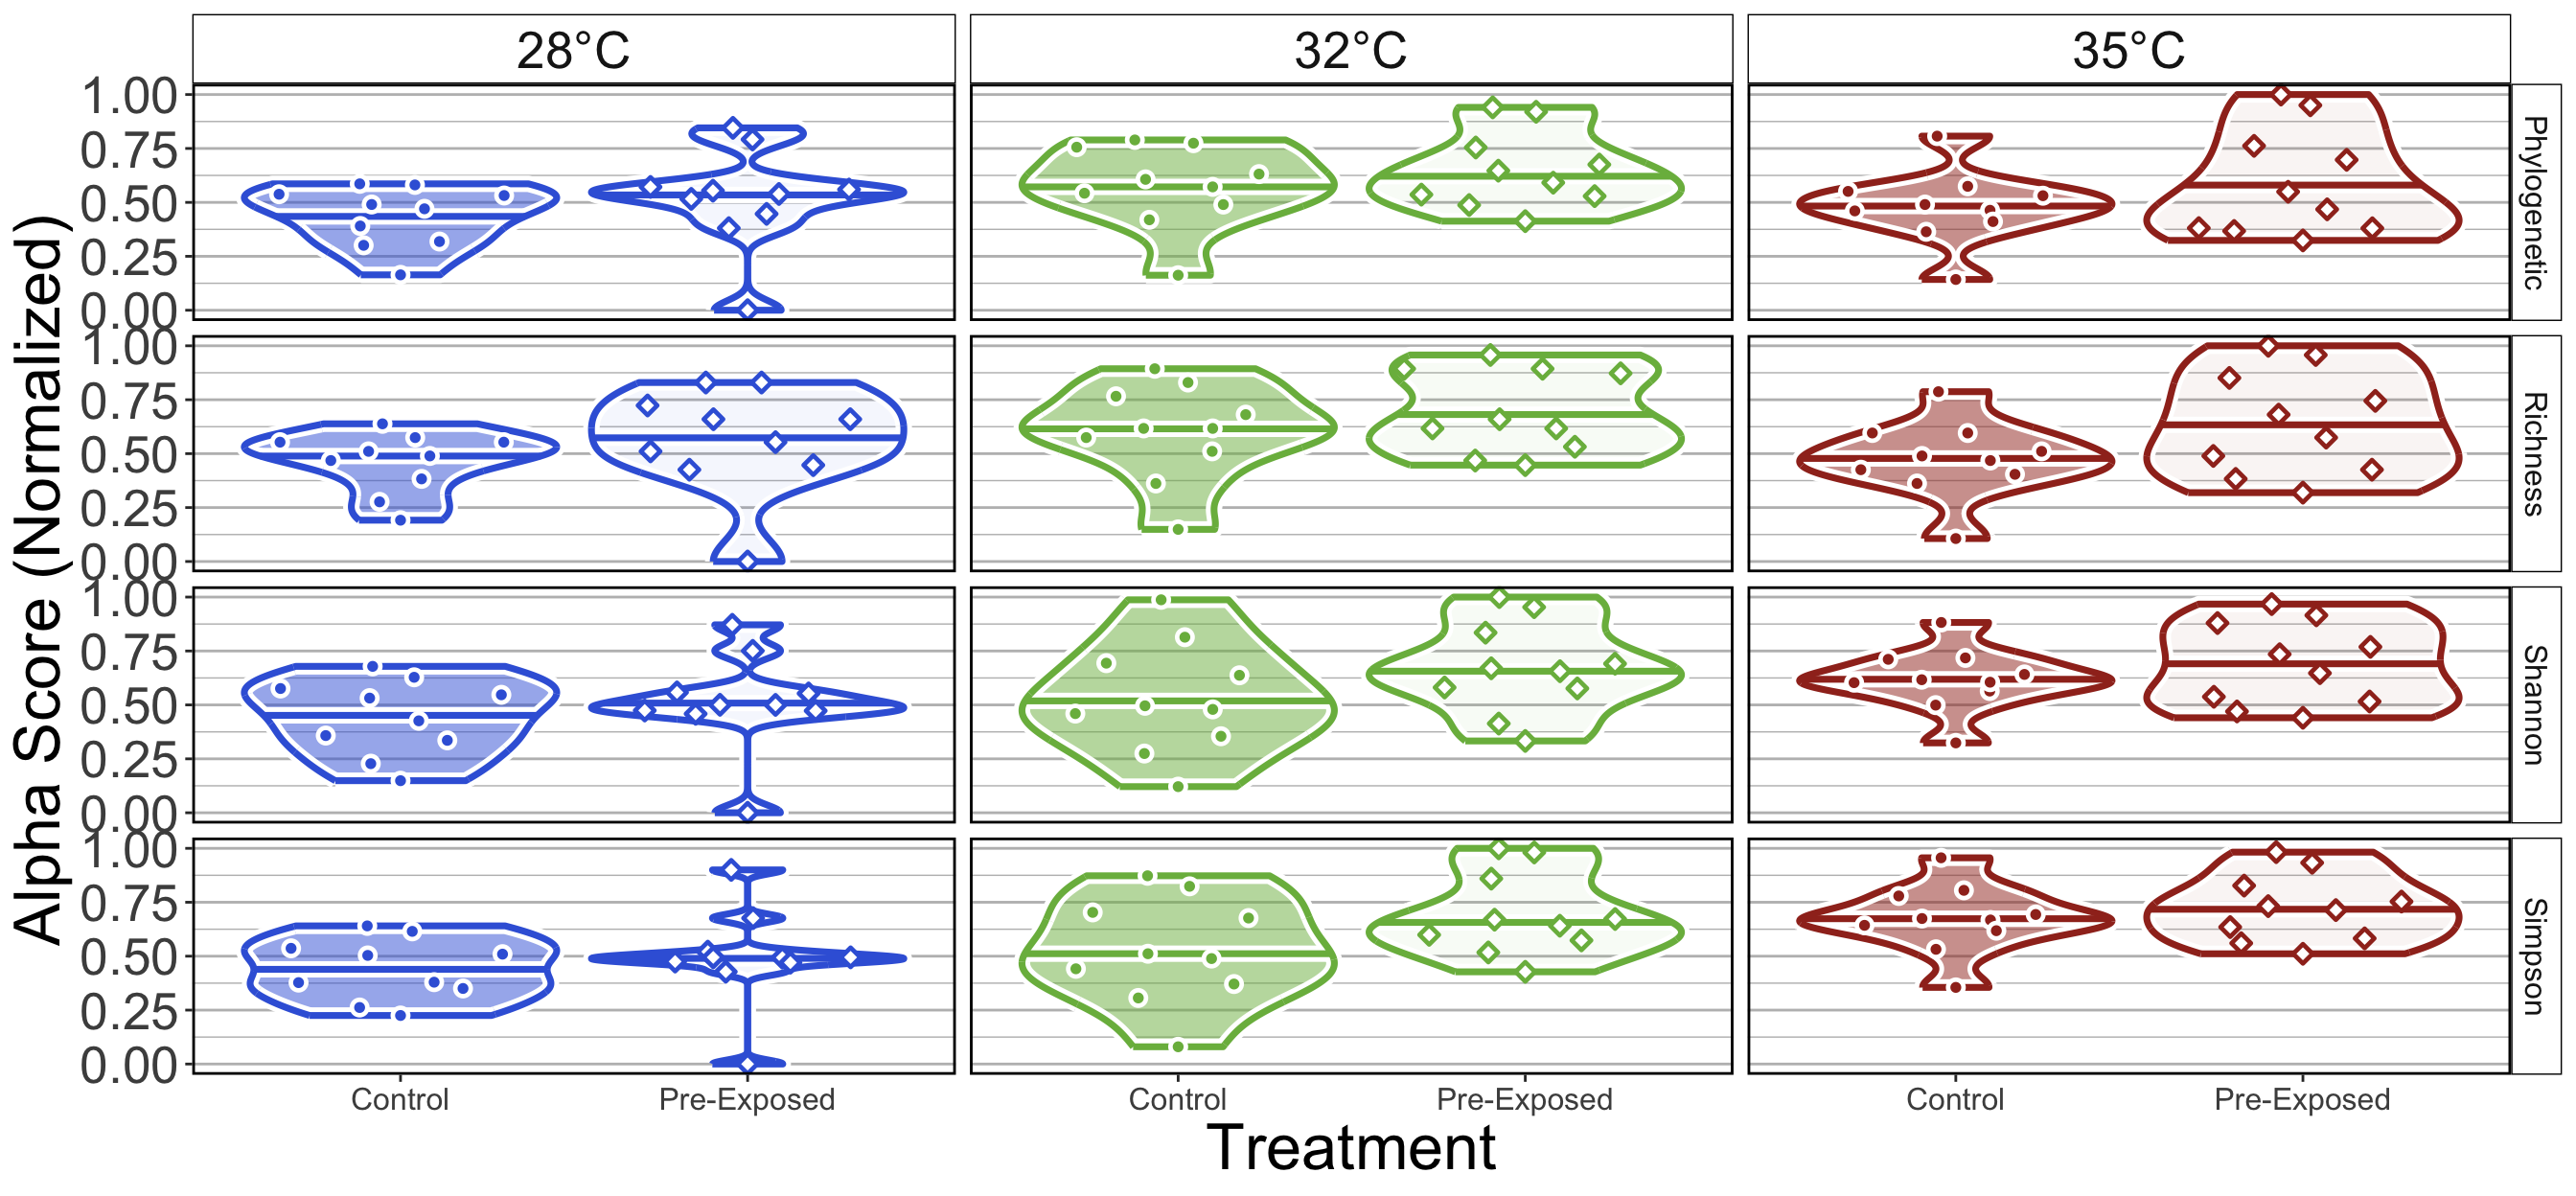
\includegraphics[keepaspectratio]{Results_Overview_files/figure-latex/plots-S6A-1.pdf}}

\paragraph{S6B}\label{s6b}

\pandocbounded{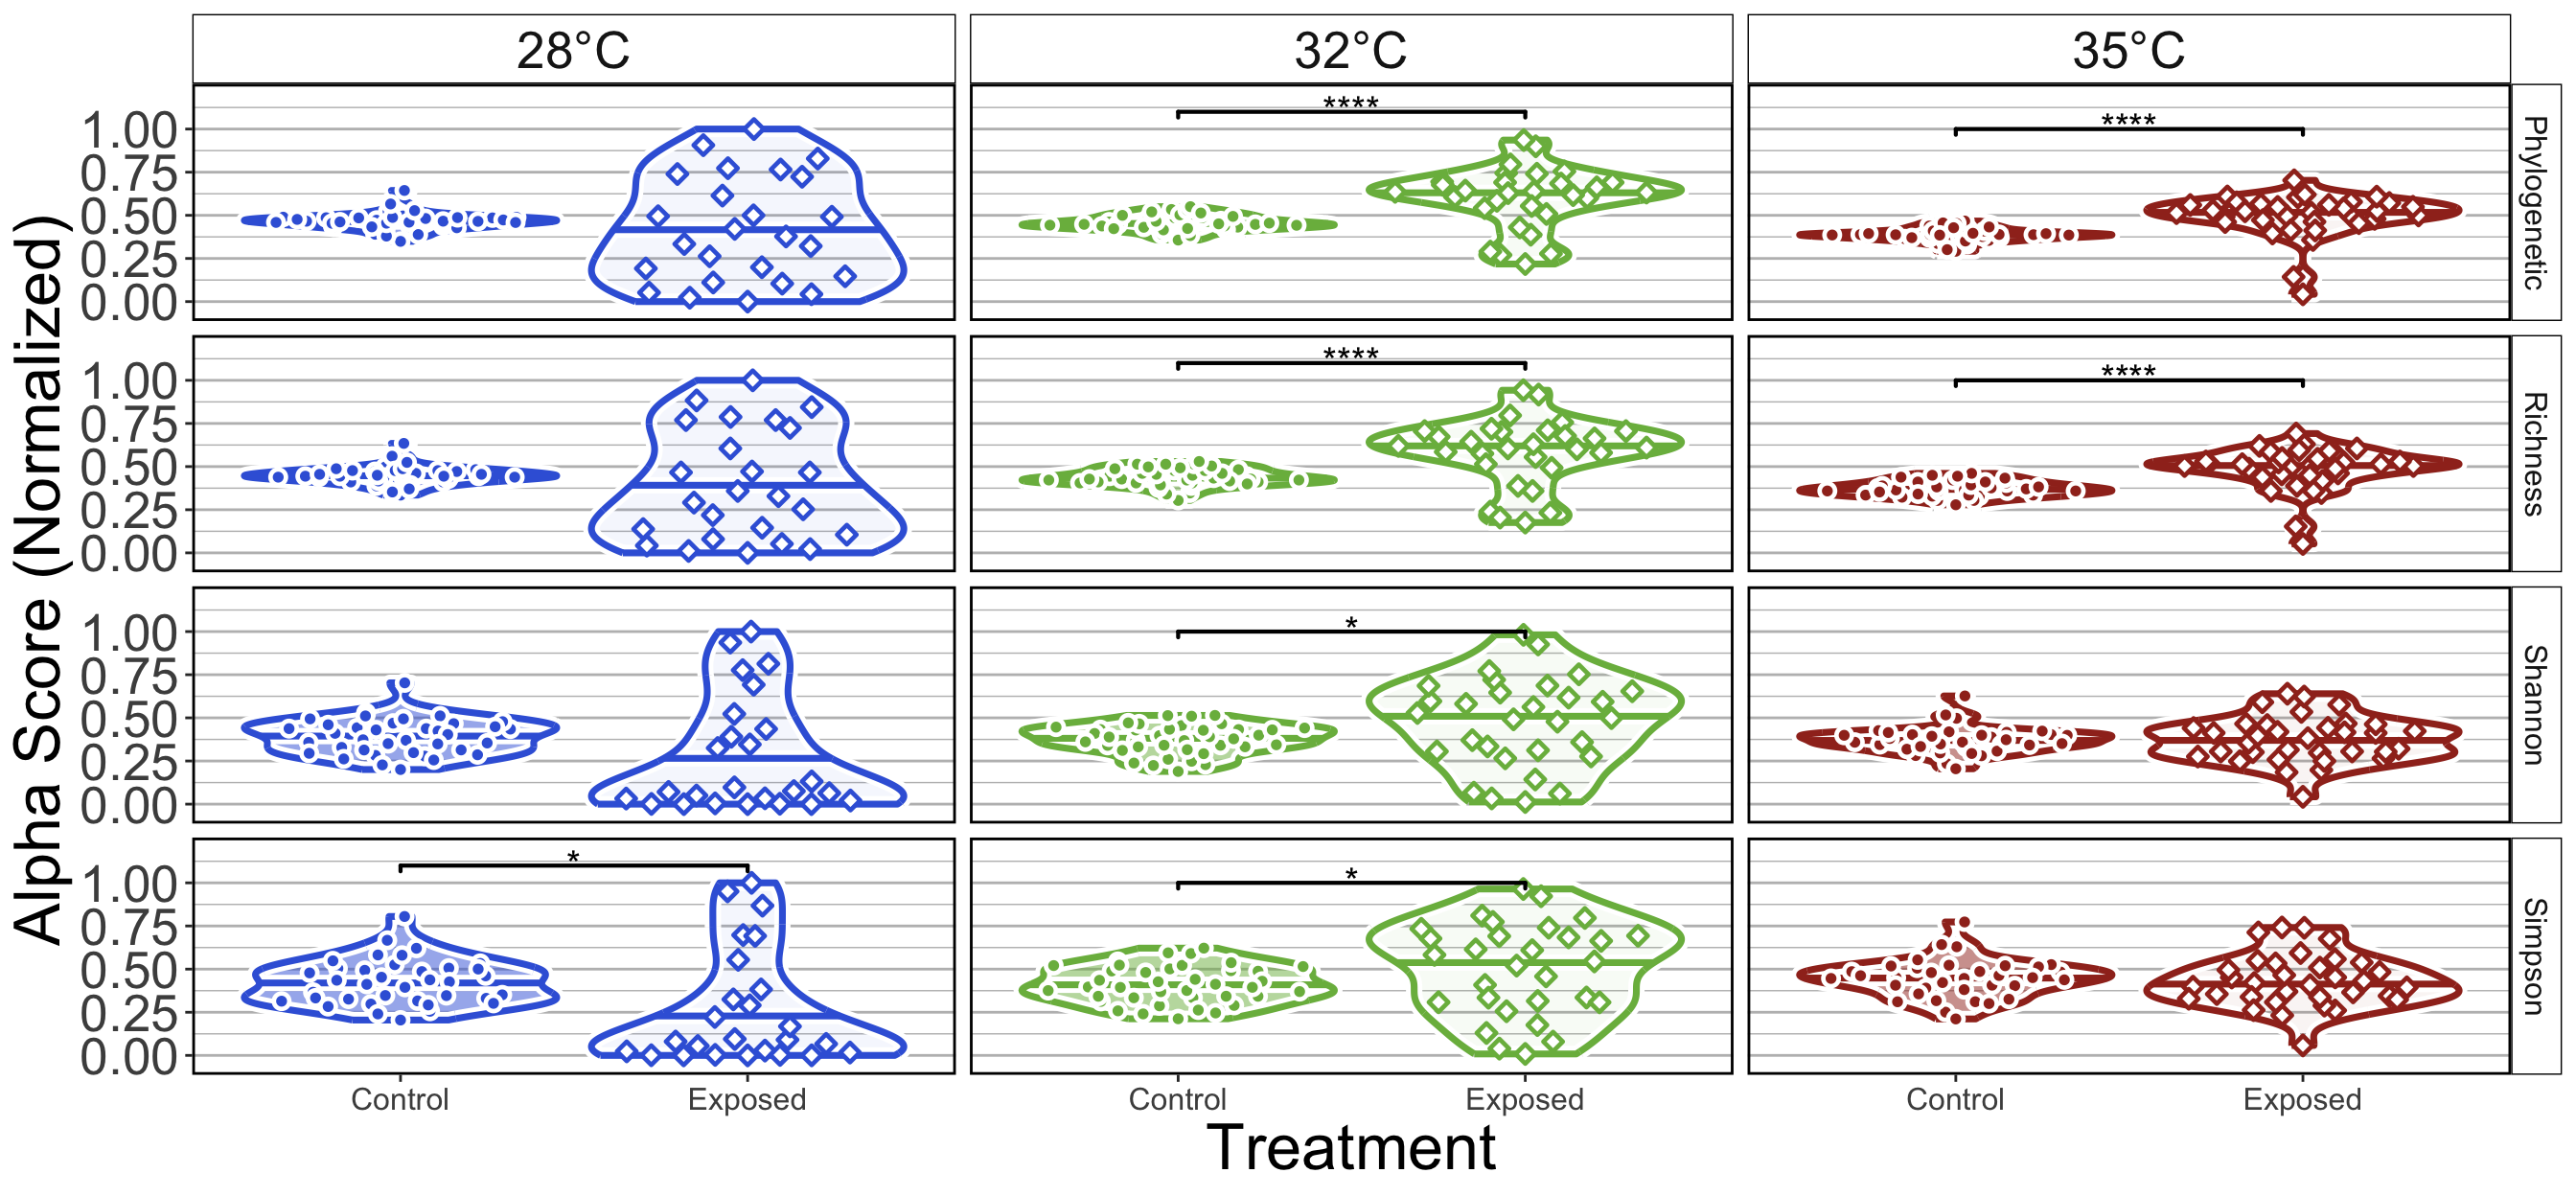
\includegraphics[keepaspectratio]{Results_Overview_files/figure-latex/plots-S6B-1.pdf}}

\paragraph{S6C}\label{s6c}

\pandocbounded{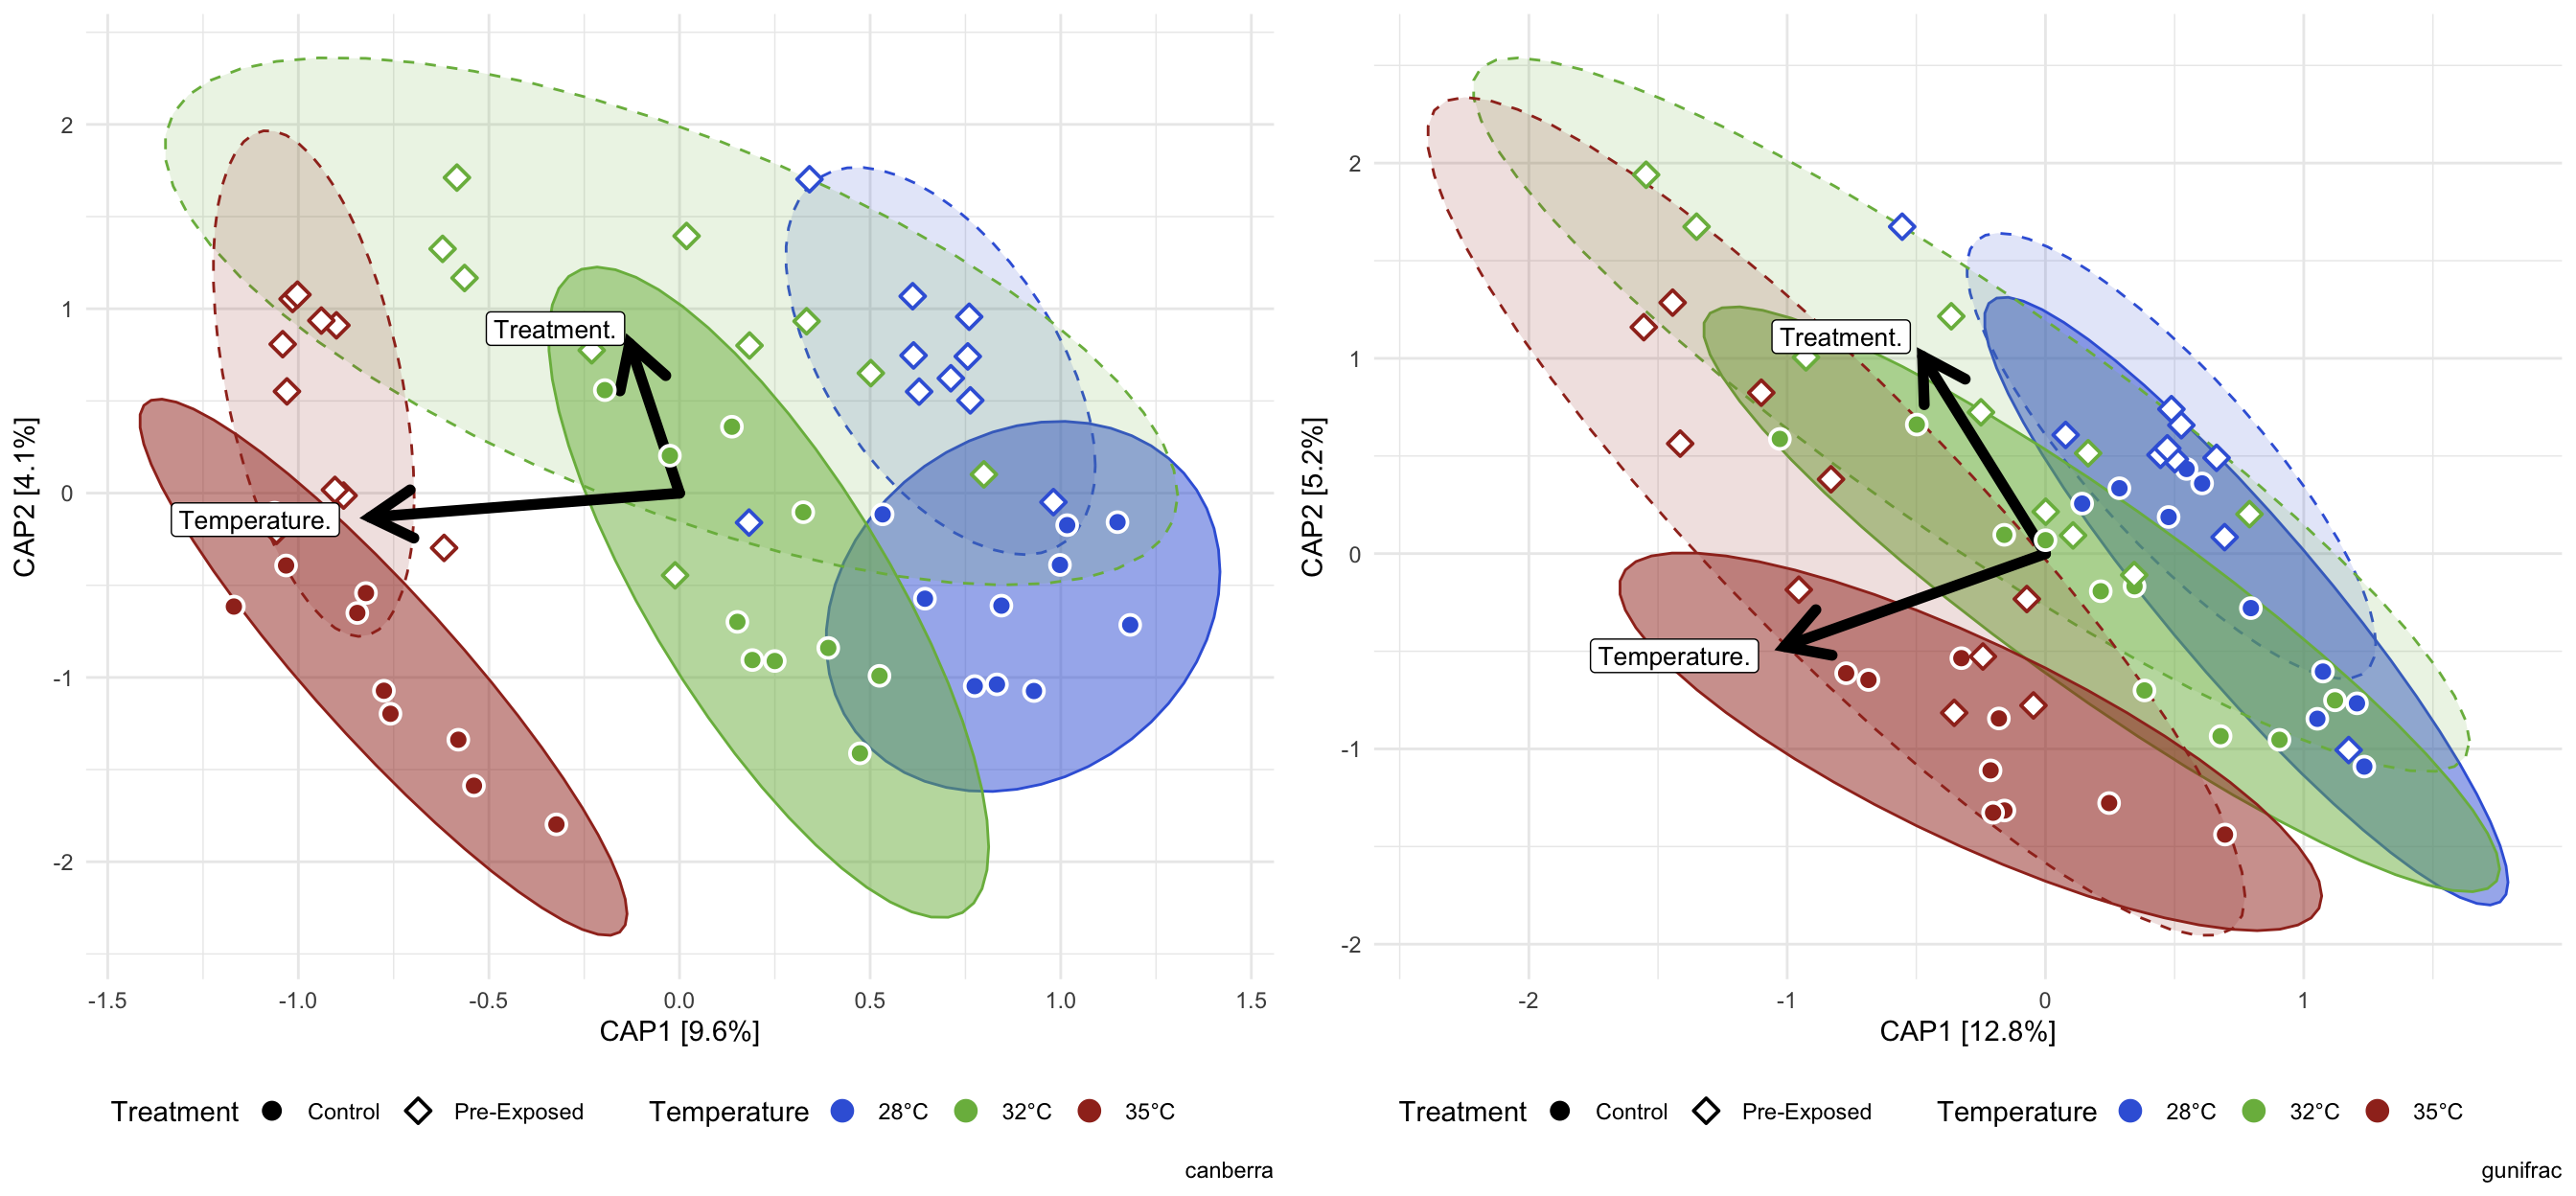
\includegraphics[keepaspectratio]{Results_Overview_files/figure-latex/plots-S6C-1.pdf}}

\subparagraph{Suppl. Plots}\label{suppl.-plots}

(hide)

Click on tabs to display tables and figures. Scroll to see additional
rows.

By Temp

\pandocbounded{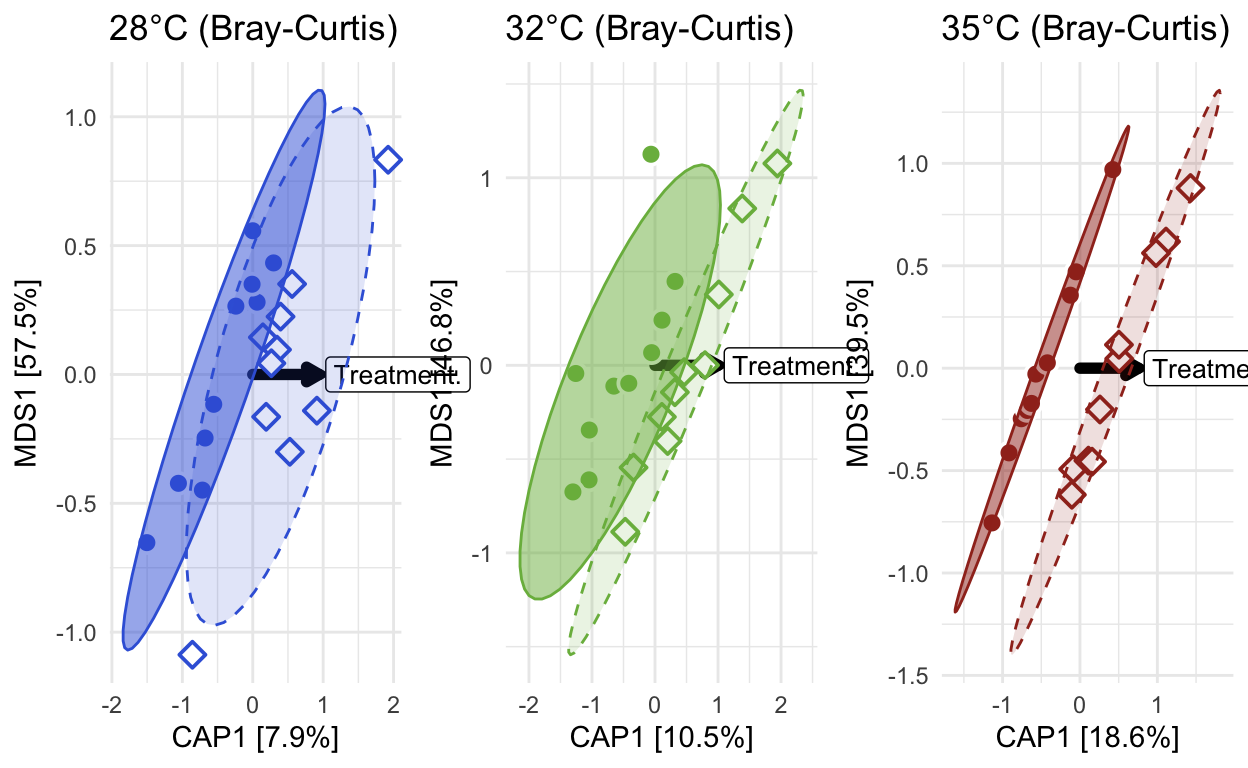
\includegraphics[keepaspectratio]{Results_Overview_files/figure-latex/plots-6C.1_byTemp-1.pdf}}
\pandocbounded{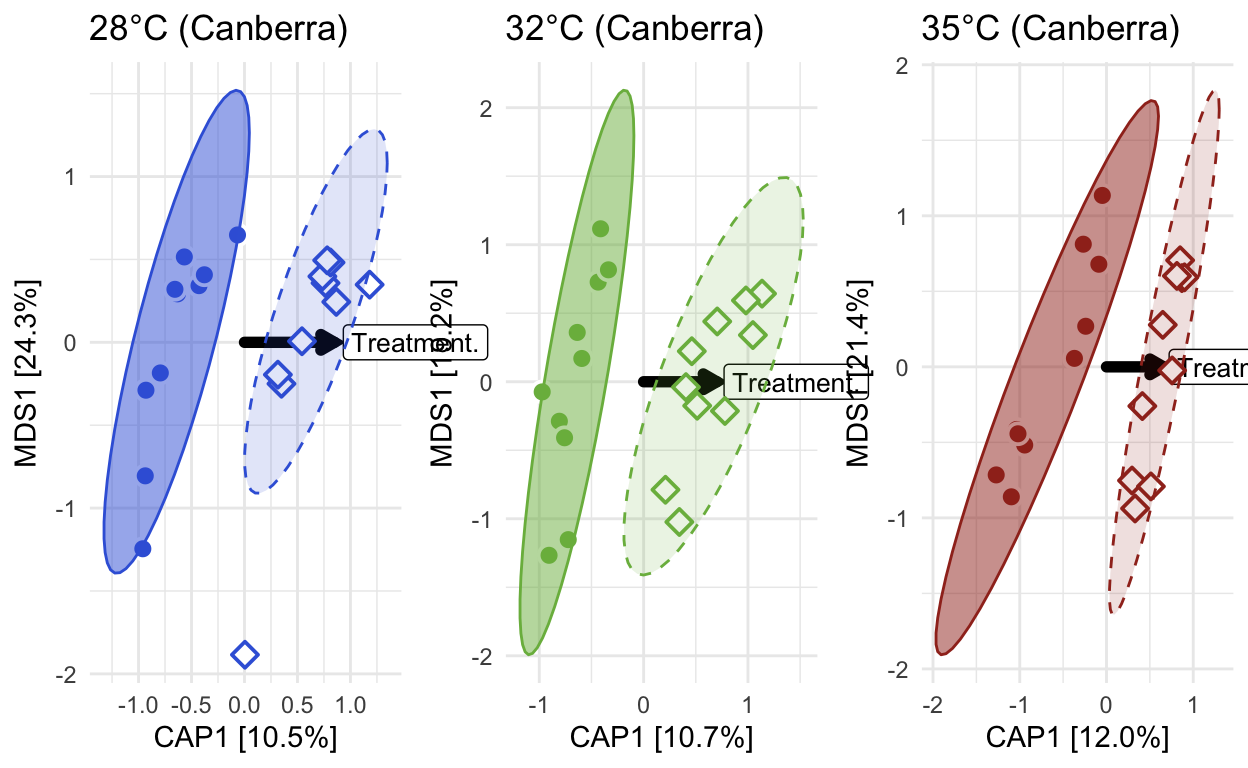
\includegraphics[keepaspectratio]{Results_Overview_files/figure-latex/plots-6C.1_byTemp-2.pdf}}
\pandocbounded{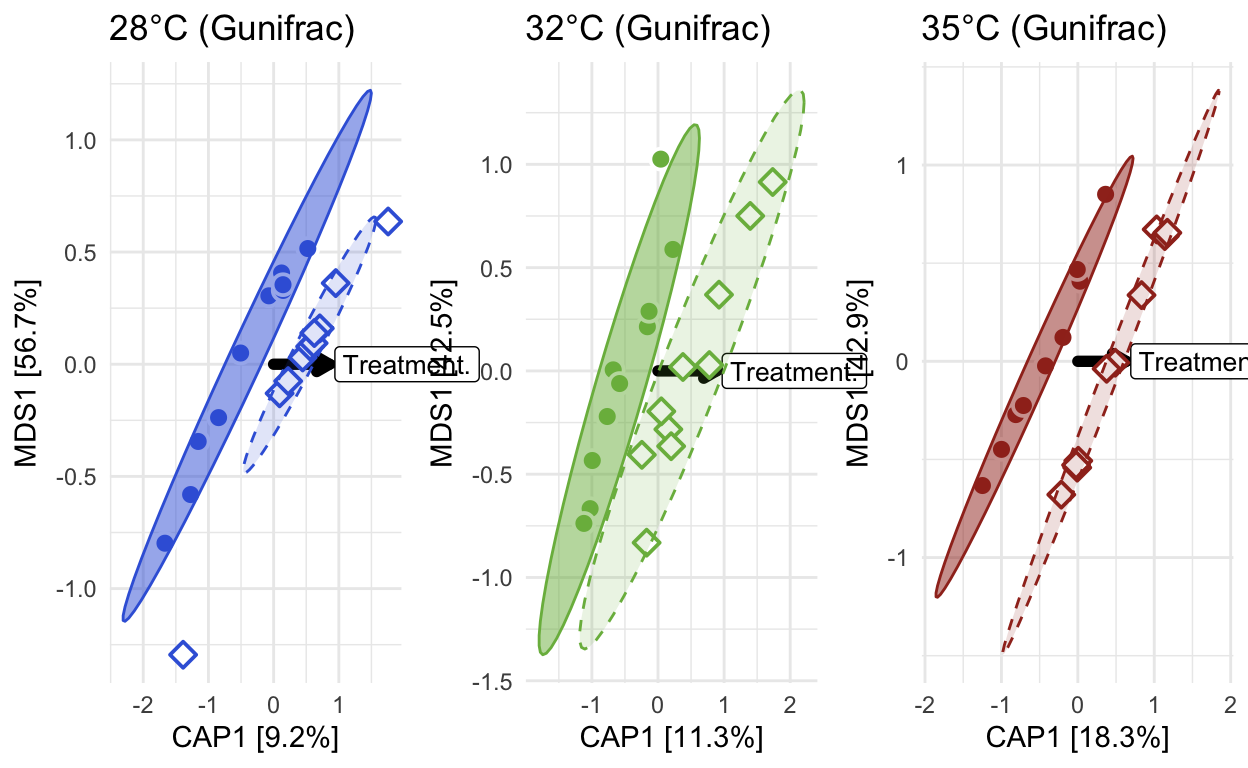
\includegraphics[keepaspectratio]{Results_Overview_files/figure-latex/plots-6C.1_byTemp-3.pdf}}

\subparagraph{Suppl. Tables}\label{suppl.-tables}

(hide)

Click on tabs to display tables and figures. Scroll to see additional
rows.

ADONIS2

\begin{longtable}{rlrrrrrl}
\toprule
Temperature & term & df & SumOfSqs & R2 & statistic & p.value & p.adj.sig \\ 
\midrule\addlinespace[2.5pt]
\multicolumn{8}{l}{bray} \\ 
\midrule\addlinespace[2.5pt]
28 & Treatment & $1.000$ & $0.065$ & $0.082$ & $1.615$ & $0.176$ & ns \\ 
28 & Residual & $18.000$ & $0.723$ & $0.918$ & NA & NA & NA \\ 
28 & Total & $19.000$ & $0.788$ & $1.000$ & NA & NA & NA \\ 
32 & Treatment & $1.000$ & $0.195$ & $0.109$ & $2.191$ & $0.087$ & ns \\ 
32 & Residual & $18.000$ & $1.603$ & $0.891$ & NA & NA & NA \\ 
32 & Total & $19.000$ & $1.799$ & $1.000$ & NA & NA & NA \\ 
35 & Treatment & $1.000$ & $0.229$ & $0.194$ & $4.346$ & $0.008$ & ** \\ 
35 & Residual & $18.000$ & $0.948$ & $0.806$ & NA & NA & NA \\ 
35 & Total & $19.000$ & $1.177$ & $1.000$ & NA & NA & NA \\ 
\midrule\addlinespace[2.5pt]
\multicolumn{8}{l}{canberra} \\ 
\midrule\addlinespace[2.5pt]
28 & Treatment & $1.000$ & $0.358$ & $0.105$ & $2.102$ & $0.010$ & * \\ 
28 & Residual & $18.000$ & $3.068$ & $0.895$ & NA & NA & NA \\ 
28 & Total & $19.000$ & $3.426$ & $1.000$ & NA & NA & NA \\ 
32 & Treatment & $1.000$ & $0.422$ & $0.107$ & $2.153$ & $0.009$ & ** \\ 
32 & Residual & $18.000$ & $3.524$ & $0.893$ & NA & NA & NA \\ 
32 & Total & $19.000$ & $3.946$ & $1.000$ & NA & NA & NA \\ 
35 & Treatment & $1.000$ & $0.421$ & $0.120$ & $2.464$ & $0.007$ & ** \\ 
35 & Residual & $18.000$ & $3.073$ & $0.880$ & NA & NA & NA \\ 
35 & Total & $19.000$ & $3.493$ & $1.000$ & NA & NA & NA \\ 
\midrule\addlinespace[2.5pt]
\multicolumn{8}{l}{gunifrac} \\ 
\midrule\addlinespace[2.5pt]
28 & Treatment & $1.000$ & $0.086$ & $0.092$ & $1.828$ & $0.130$ & ns \\ 
28 & Residual & $18.000$ & $0.845$ & $0.908$ & NA & NA & NA \\ 
28 & Total & $19.000$ & $0.931$ & $1.000$ & NA & NA & NA \\ 
32 & Treatment & $1.000$ & $0.174$ & $0.113$ & $2.296$ & $0.062$ & ns \\ 
32 & Residual & $18.000$ & $1.361$ & $0.887$ & NA & NA & NA \\ 
32 & Total & $19.000$ & $1.535$ & $1.000$ & NA & NA & NA \\ 
35 & Treatment & $1.000$ & $0.206$ & $0.184$ & $4.068$ & $0.012$ & * \\ 
35 & Residual & $18.000$ & $0.911$ & $0.816$ & NA & NA & NA \\ 
35 & Total & $19.000$ & $1.117$ & $1.000$ & NA & NA & NA \\ 
\bottomrule
\end{longtable}

Dispersion (ANOVA)

\begin{longtable}{rlrrrrrl}
\toprule
Temperature & term & df & sumsq & meansq & statistic & p.value & p.adj.sig \\ 
\midrule\addlinespace[2.5pt]
\multicolumn{8}{l}{bray} \\ 
\midrule\addlinespace[2.5pt]
28 & Groups & $1.000$ & $0.004$ & $0.004$ & $0.609$ & $0.445$ & ns \\ 
28 & Residuals & $18.000$ & $0.105$ & $0.006$ & NA & NA & NA \\ 
32 & Groups & $1.000$ & $0.001$ & $0.001$ & $0.100$ & $0.755$ & ns \\ 
32 & Residuals & $18.000$ & $0.199$ & $0.011$ & NA & NA & NA \\ 
35 & Groups & $1.000$ & $0.014$ & $0.014$ & $2.589$ & $0.125$ & ns \\ 
35 & Residuals & $18.000$ & $0.101$ & $0.006$ & NA & NA & NA \\ 
\midrule\addlinespace[2.5pt]
\multicolumn{8}{l}{canberra} \\ 
\midrule\addlinespace[2.5pt]
28 & Groups & $1.000$ & $0.001$ & $0.001$ & $0.061$ & $0.807$ & ns \\ 
28 & Residuals & $18.000$ & $0.172$ & $0.010$ & NA & NA & NA \\ 
32 & Groups & $1.000$ & $0.000$ & $0.000$ & $0.078$ & $0.783$ & ns \\ 
32 & Residuals & $18.000$ & $0.092$ & $0.005$ & NA & NA & NA \\ 
35 & Groups & $1.000$ & $0.000$ & $0.000$ & $0.055$ & $0.817$ & ns \\ 
35 & Residuals & $18.000$ & $0.065$ & $0.004$ & NA & NA & NA \\ 
\midrule\addlinespace[2.5pt]
\multicolumn{8}{l}{gunifrac} \\ 
\midrule\addlinespace[2.5pt]
28 & Groups & $1.000$ & $0.000$ & $0.000$ & $0.004$ & $0.948$ & ns \\ 
28 & Residuals & $18.000$ & $0.165$ & $0.009$ & NA & NA & NA \\ 
32 & Groups & $1.000$ & $0.003$ & $0.003$ & $0.465$ & $0.504$ & ns \\ 
32 & Residuals & $18.000$ & $0.135$ & $0.008$ & NA & NA & NA \\ 
35 & Groups & $1.000$ & $0.009$ & $0.009$ & $2.238$ & $0.152$ & ns \\ 
35 & Residuals & $18.000$ & $0.069$ & $0.004$ & NA & NA & NA \\ 
\bottomrule
\end{longtable}

\paragraph{S6D}\label{s6d}

\pandocbounded{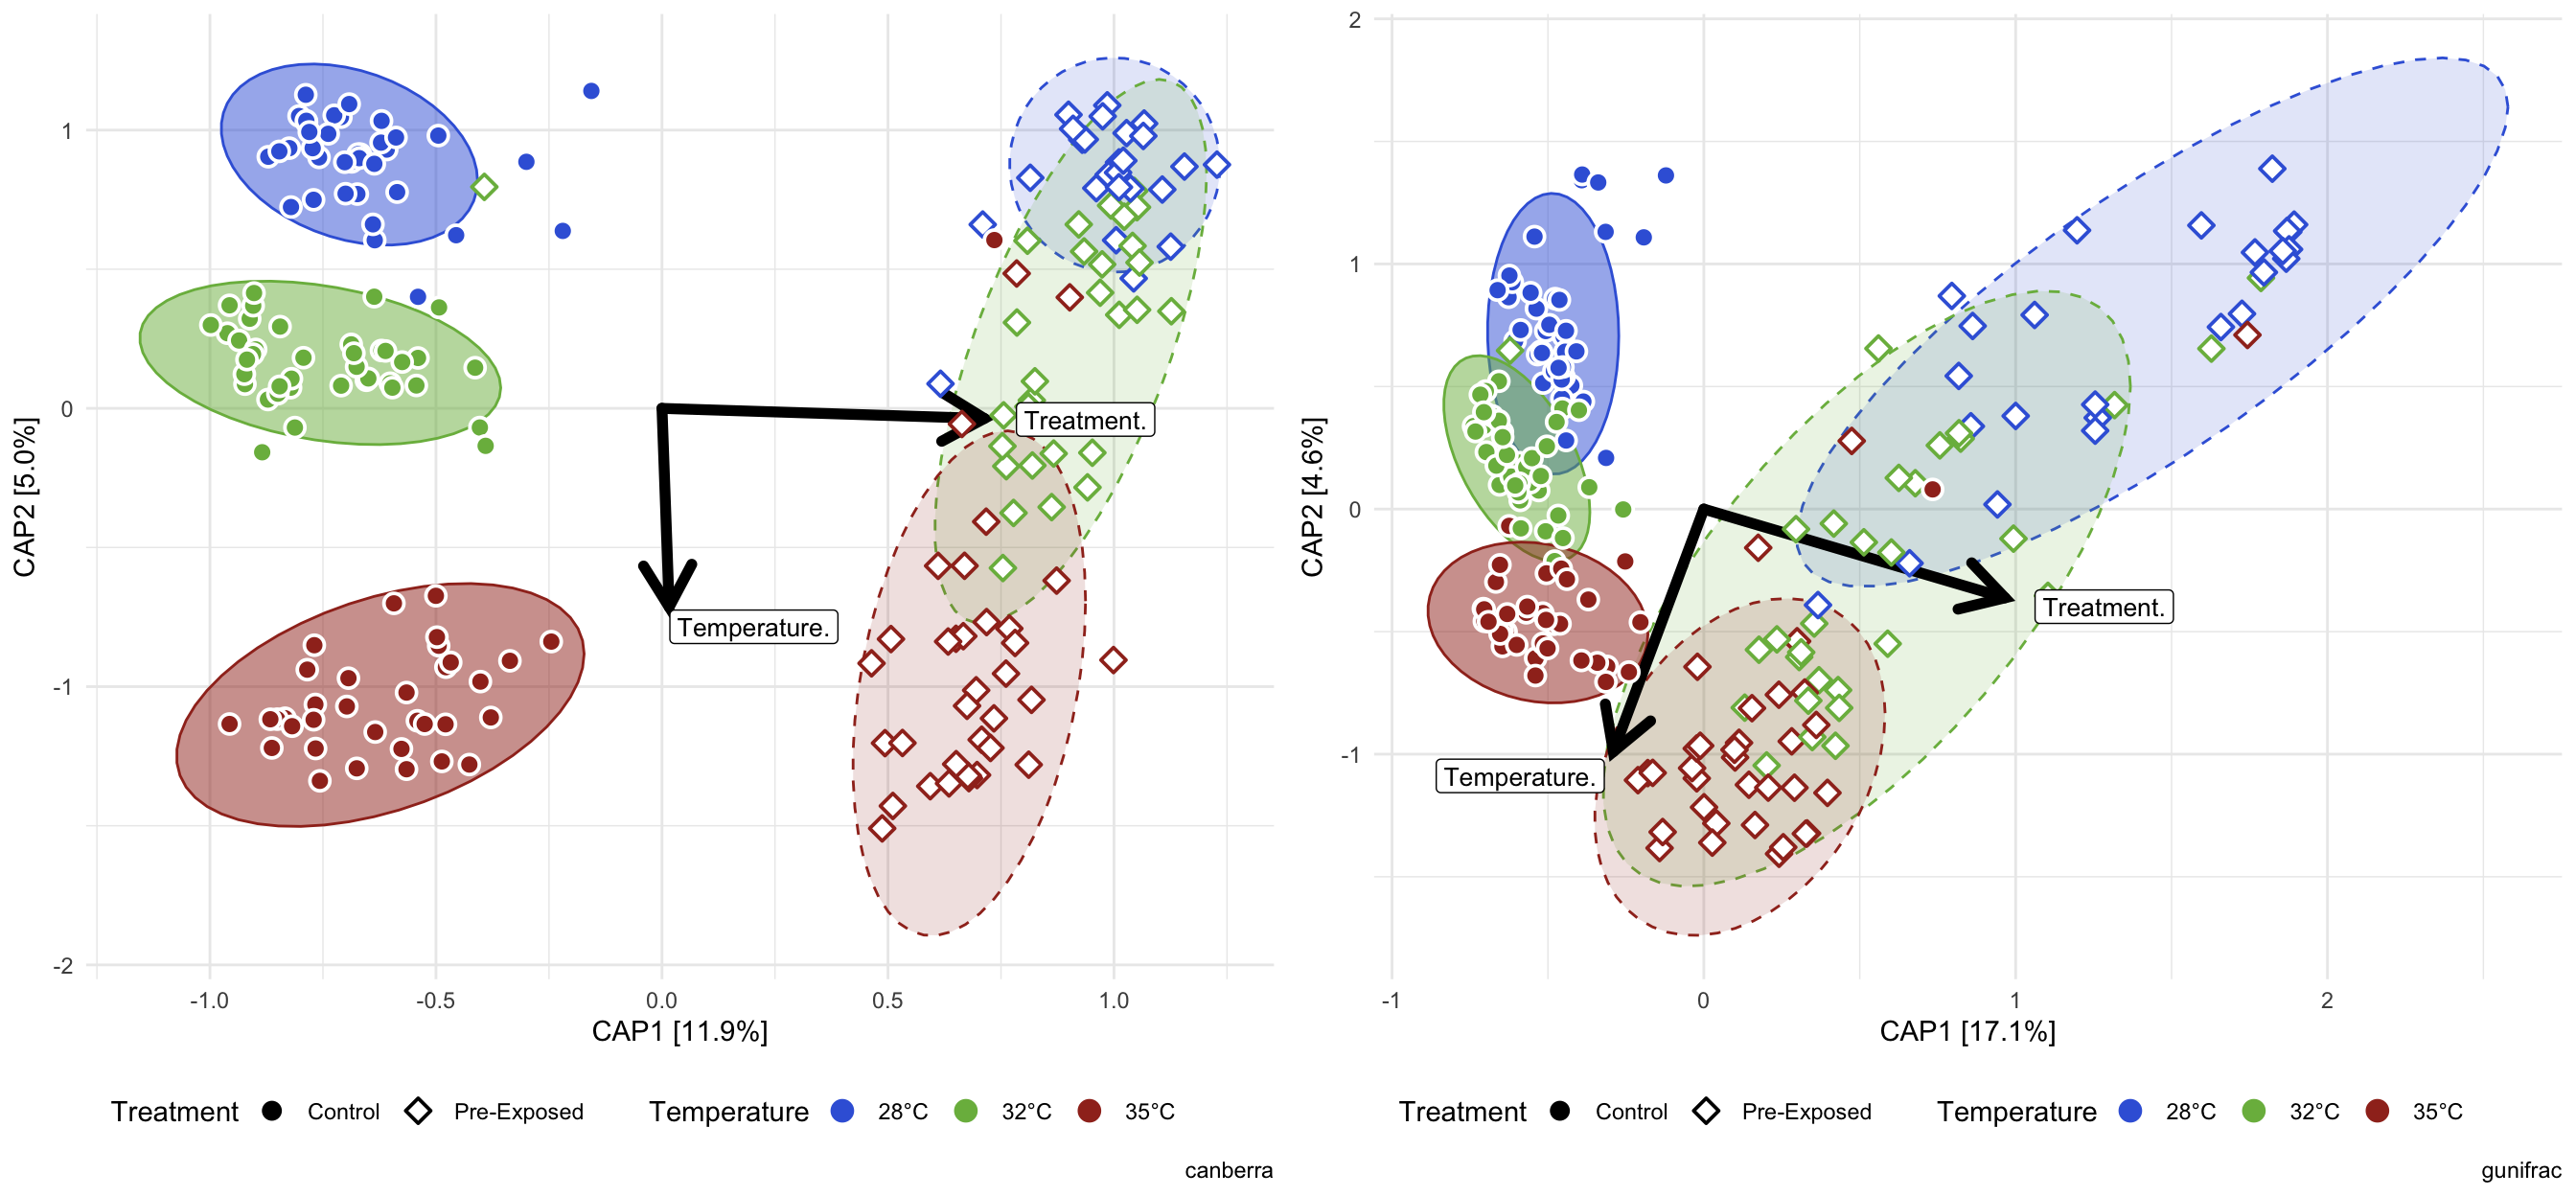
\includegraphics[keepaspectratio]{Results_Overview_files/figure-latex/plots-S6D-1.pdf}}

\subparagraph{Suppl. Plots}\label{suppl.-plots-1}

(hide)

Click on tabs to display tables and figures. Scroll to see additional
rows.

By Temp

\pandocbounded{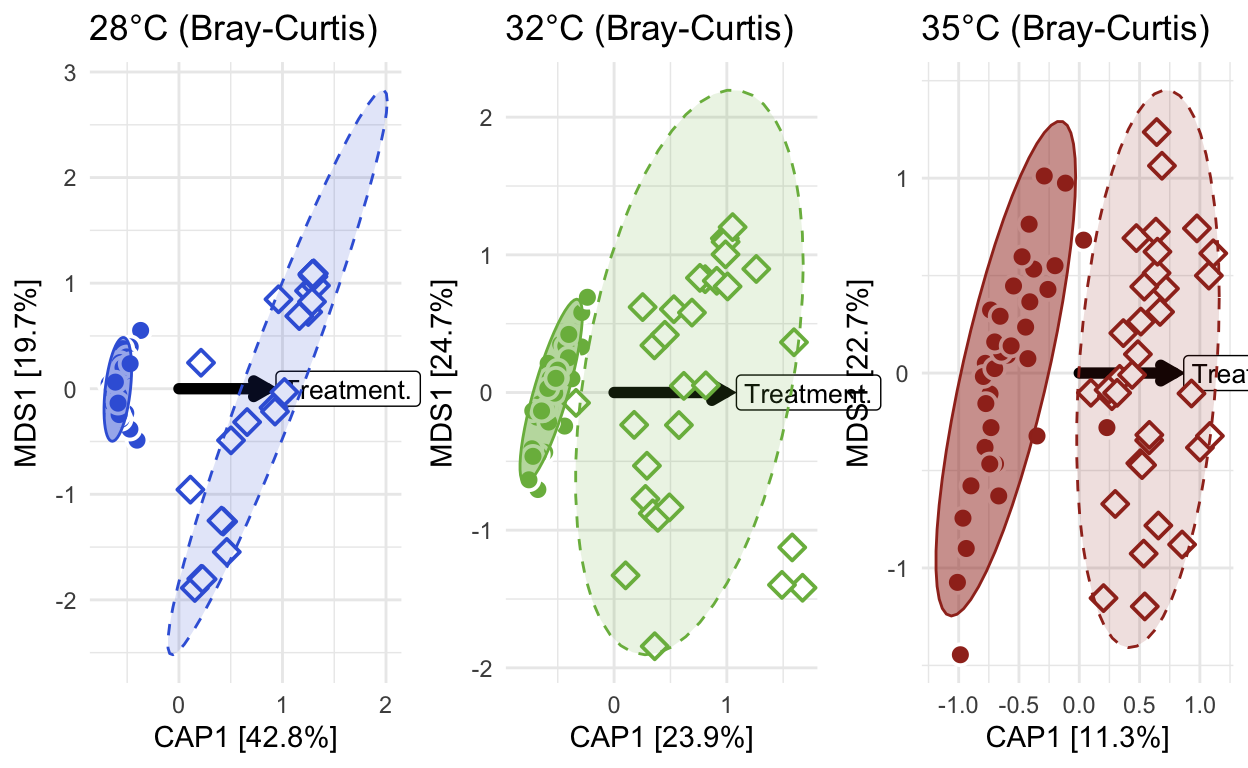
\includegraphics[keepaspectratio]{Results_Overview_files/figure-latex/plots-6D.1_byTemp-1.pdf}}
\pandocbounded{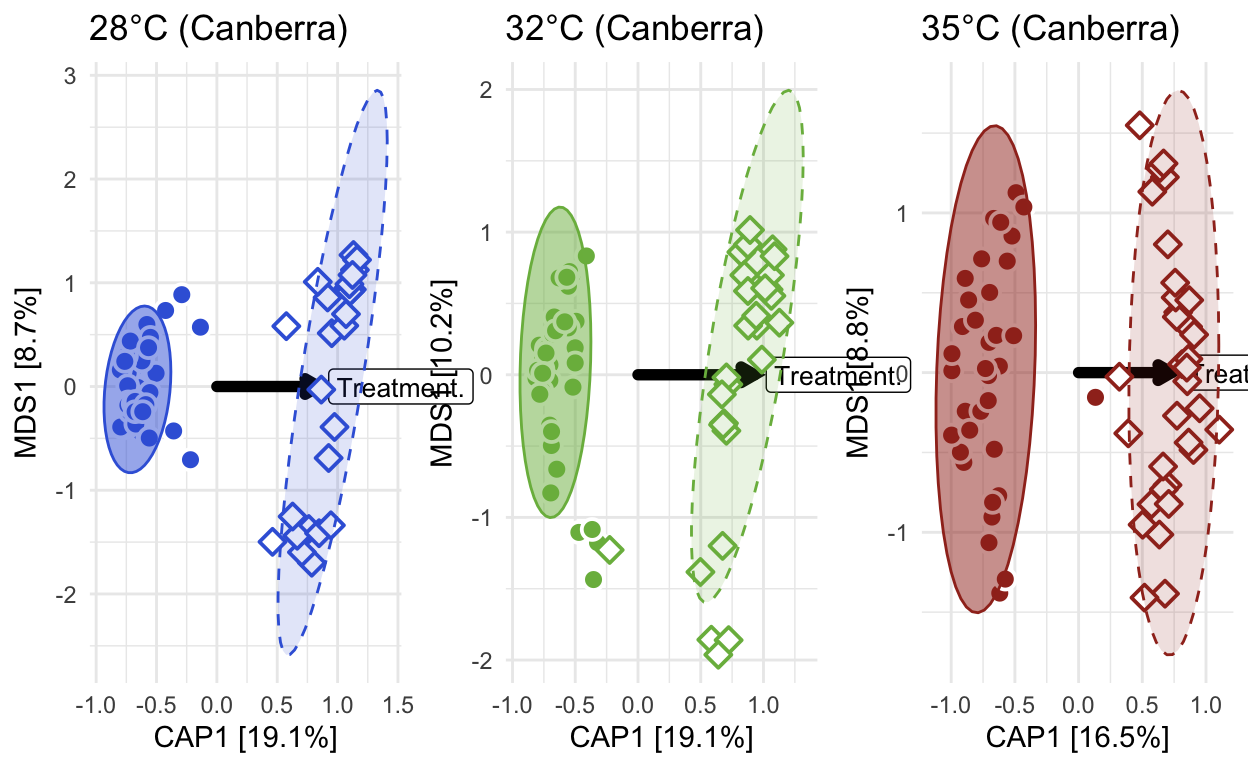
\includegraphics[keepaspectratio]{Results_Overview_files/figure-latex/plots-6D.1_byTemp-2.pdf}}
\pandocbounded{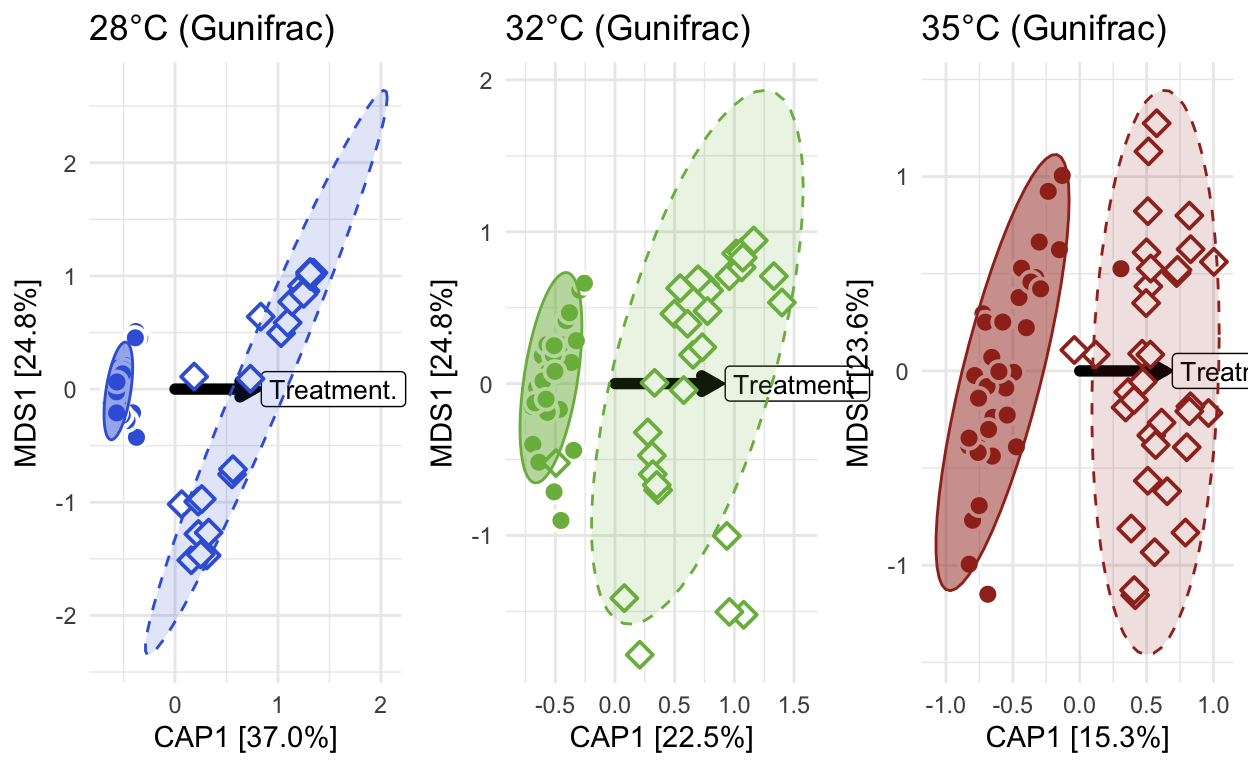
\includegraphics[keepaspectratio]{Results_Overview_files/figure-latex/plots-6D.1_byTemp-3.pdf}}

\subparagraph{Suppl. Tables}\label{suppl.-tables-1}

(hide)

Click on tabs to display tables and figures. Scroll to see additional
rows.

ADONIS2

\begin{longtable}{rlrrrrrr}
\toprule
Temperature & term & df & SumOfSqs & R2 & statistic & p.value & p.adj.sig \\ 
\midrule\addlinespace[2.5pt]
\multicolumn{8}{l}{bray} \\ 
\midrule\addlinespace[2.5pt]
28 & Treatment & $1.000$ & $6.719$ & $0.447$ & $48.541$ & $0.001$ & ** \\ 
28 & Residual & $60.000$ & $8.305$ & $0.553$ & NA & NA & NA \\ 
28 & Total & $61.000$ & $15.023$ & $1.000$ & NA & NA & NA \\ 
32 & Treatment & $1.000$ & $2.842$ & $0.261$ & $23.668$ & $0.001$ & ** \\ 
32 & Residual & $67.000$ & $8.044$ & $0.739$ & NA & NA & NA \\ 
32 & Total & $68.000$ & $10.886$ & $1.000$ & NA & NA & NA \\ 
35 & Treatment & $1.000$ & $1.018$ & $0.125$ & $9.568$ & $0.001$ & ** \\ 
35 & Residual & $67.000$ & $7.129$ & $0.875$ & NA & NA & NA \\ 
35 & Total & $68.000$ & $8.147$ & $1.000$ & NA & NA & NA \\ 
\midrule\addlinespace[2.5pt]
\multicolumn{8}{l}{canberra} \\ 
\midrule\addlinespace[2.5pt]
28 & Treatment & $1.000$ & $3.887$ & $0.191$ & $14.144$ & $0.001$ & ** \\ 
28 & Residual & $60.000$ & $16.490$ & $0.809$ & NA & NA & NA \\ 
28 & Total & $61.000$ & $20.377$ & $1.000$ & NA & NA & NA \\ 
32 & Treatment & $1.000$ & $3.542$ & $0.191$ & $15.809$ & $0.001$ & ** \\ 
32 & Residual & $67.000$ & $15.012$ & $0.809$ & NA & NA & NA \\ 
32 & Total & $68.000$ & $18.554$ & $1.000$ & NA & NA & NA \\ 
35 & Treatment & $1.000$ & $2.987$ & $0.165$ & $13.288$ & $0.001$ & ** \\ 
35 & Residual & $67.000$ & $15.059$ & $0.835$ & NA & NA & NA \\ 
35 & Total & $68.000$ & $18.046$ & $1.000$ & NA & NA & NA \\ 
\midrule\addlinespace[2.5pt]
\multicolumn{8}{l}{gunifrac} \\ 
\midrule\addlinespace[2.5pt]
28 & Treatment & $1.000$ & $4.085$ & $0.374$ & $35.857$ & $0.001$ & ** \\ 
28 & Residual & $60.000$ & $6.836$ & $0.626$ & NA & NA & NA \\ 
28 & Total & $61.000$ & $10.922$ & $1.000$ & NA & NA & NA \\ 
32 & Treatment & $1.000$ & $2.031$ & $0.230$ & $19.988$ & $0.001$ & ** \\ 
32 & Residual & $67.000$ & $6.806$ & $0.770$ & NA & NA & NA \\ 
32 & Total & $68.000$ & $8.837$ & $1.000$ & NA & NA & NA \\ 
35 & Treatment & $1.000$ & $1.080$ & $0.160$ & $12.720$ & $0.001$ & ** \\ 
35 & Residual & $67.000$ & $5.691$ & $0.840$ & NA & NA & NA \\ 
35 & Total & $68.000$ & $6.771$ & $1.000$ & NA & NA & NA \\ 
\bottomrule
\end{longtable}

Dispersion (ANOVA)

\begin{longtable}{rlrrrrrl}
\toprule
Temperature & term & df & sumsq & meansq & statistic & p.value & p.adj.sig \\ 
\midrule\addlinespace[2.5pt]
\multicolumn{8}{l}{bray} \\ 
\midrule\addlinespace[2.5pt]
28 & Groups & $1.000$ & $0.662$ & $0.662$ & $53.570$ & $0.000$ & **** \\ 
28 & Residuals & $60.000$ & $0.741$ & $0.012$ & NA & NA & NA \\ 
32 & Groups & $1.000$ & $0.567$ & $0.567$ & $54.435$ & $0.000$ & **** \\ 
32 & Residuals & $67.000$ & $0.697$ & $0.010$ & NA & NA & NA \\ 
35 & Groups & $1.000$ & $0.038$ & $0.038$ & $1.735$ & $0.192$ & ns \\ 
35 & Residuals & $67.000$ & $1.479$ & $0.022$ & NA & NA & NA \\ 
\midrule\addlinespace[2.5pt]
\multicolumn{8}{l}{canberra} \\ 
\midrule\addlinespace[2.5pt]
28 & Groups & $1.000$ & $0.703$ & $0.703$ & $224.734$ & $0.000$ & **** \\ 
28 & Residuals & $60.000$ & $0.188$ & $0.003$ & NA & NA & NA \\ 
32 & Groups & $1.000$ & $0.237$ & $0.237$ & $30.033$ & $0.000$ & **** \\ 
32 & Residuals & $67.000$ & $0.530$ & $0.008$ & NA & NA & NA \\ 
35 & Groups & $1.000$ & $0.062$ & $0.062$ & $6.749$ & $0.012$ & * \\ 
35 & Residuals & $67.000$ & $0.620$ & $0.009$ & NA & NA & NA \\ 
\midrule\addlinespace[2.5pt]
\multicolumn{8}{l}{gunifrac} \\ 
\midrule\addlinespace[2.5pt]
28 & Groups & $1.000$ & $0.582$ & $0.582$ & $124.383$ & $0.000$ & **** \\ 
28 & Residuals & $60.000$ & $0.281$ & $0.005$ & NA & NA & NA \\ 
32 & Groups & $1.000$ & $0.482$ & $0.482$ & $57.322$ & $0.000$ & **** \\ 
32 & Residuals & $67.000$ & $0.564$ & $0.008$ & NA & NA & NA \\ 
35 & Groups & $1.000$ & $0.078$ & $0.078$ & $5.842$ & $0.018$ & * \\ 
35 & Residuals & $67.000$ & $0.896$ & $0.013$ & NA & NA & NA \\ 
\bottomrule
\end{longtable}

\subsubsection{Fig. 7) Gut microbial abundance is significantly
associated with environmental conditions and
stressors}\label{fig.-7-gut-microbial-abundance-is-significantly-associated-with-environmental-conditions-and-stressors}

\paragraph{7) Gut microbial abundance is significantly associated with
environmental conditions and
stressors}\label{gut-microbial-abundance-is-significantly-associated-with-environmental-conditions-and-stressors}

\textbf{Fig. 7} A heatmap of model coefficient values of the top 50
statistically significant abundant gut microbial taxa identified by
MaAsLin2. The color of each cell represents the coefficient value and
direction (red is positive, blue is negative). A ``+'' or ``-''
indicates a statistically significant association was observed between
taxon abundance and a covariate. Gray colored cells indicate a
significant effect was not observed.

\begin{longtable}{lrrrrrrr}
\toprule
Taxon & Temp: 32°C & Temp: 35°C & Time (DPE) & Cluster: Low & Parasite exposed & Infection present & Infection burden \\ 
\midrule\addlinespace[2.5pt]
\multicolumn{8}{l}{Actinobacteriota} \\ 
\midrule\addlinespace[2.5pt]
IMCC26207 & \cellcolor[HTML]{FFDDD1}{\textcolor[HTML]{000000}{\textbf{+}}} & \cellcolor[HTML]{F2F2F2}{\textcolor[HTML]{000000}{}} & \cellcolor[HTML]{FEFDFF}{\textcolor[HTML]{000000}{\textbf{-}}} & \cellcolor[HTML]{D5BAFF}{\textcolor[HTML]{000000}{\textbf{-}}} & \cellcolor[HTML]{C9A8FF}{\textcolor[HTML]{000000}{\textbf{-}}} & \cellcolor[HTML]{F2F2F2}{\textcolor[HTML]{000000}{}} & \cellcolor[HTML]{F2F2F2}{\textcolor[HTML]{000000}{}} \\ 
Nocardiaceae Genus & \cellcolor[HTML]{FFD6C8}{\textcolor[HTML]{000000}{\textbf{+}}} & \cellcolor[HTML]{FF9678}{\textcolor[HTML]{000000}{\textbf{+}}} & \cellcolor[HTML]{FFFDFC}{\textcolor[HTML]{000000}{\textbf{+}}} & \cellcolor[HTML]{F2F2F2}{\textcolor[HTML]{000000}{}} & \cellcolor[HTML]{F2F2F2}{\textcolor[HTML]{000000}{}} & \cellcolor[HTML]{F2F2F2}{\textcolor[HTML]{000000}{}} & \cellcolor[HTML]{F2F2F2}{\textcolor[HTML]{000000}{}} \\ 
PeM15 Genus & \cellcolor[HTML]{FFEAE3}{\textcolor[HTML]{000000}{\textbf{+}}} & \cellcolor[HTML]{F2F2F2}{\textcolor[HTML]{000000}{}} & \cellcolor[HTML]{FEFDFF}{\textcolor[HTML]{000000}{\textbf{-}}} & \cellcolor[HTML]{C4A1FF}{\textcolor[HTML]{000000}{\textbf{-}}} & \cellcolor[HTML]{B993FF}{\textcolor[HTML]{000000}{\textbf{-}}} & \cellcolor[HTML]{F2F2F2}{\textcolor[HTML]{000000}{}} & \cellcolor[HTML]{F2F2F2}{\textcolor[HTML]{000000}{}} \\ 
\midrule\addlinespace[2.5pt]
\multicolumn{8}{l}{Bacteroidota} \\ 
\midrule\addlinespace[2.5pt]
Barnesiellaceae Genus & \cellcolor[HTML]{F2F2F2}{\textcolor[HTML]{000000}{}} & \cellcolor[HTML]{F2F2F2}{\textcolor[HTML]{000000}{}} & \cellcolor[HTML]{FCF9FF}{\textcolor[HTML]{000000}{\textbf{-}}} & \cellcolor[HTML]{F2F2F2}{\textcolor[HTML]{000000}{}} & \cellcolor[HTML]{CCACFF}{\textcolor[HTML]{000000}{\textbf{-}}} & \cellcolor[HTML]{F2F2F2}{\textcolor[HTML]{000000}{}} & \cellcolor[HTML]{F2F2F2}{\textcolor[HTML]{000000}{}} \\ 
Cloacibacterium & \cellcolor[HTML]{F2F2F2}{\textcolor[HTML]{000000}{}} & \cellcolor[HTML]{FFE8E0}{\textcolor[HTML]{000000}{\textbf{+}}} & \cellcolor[HTML]{FDFCFF}{\textcolor[HTML]{000000}{\textbf{-}}} & \cellcolor[HTML]{F2F2F2}{\textcolor[HTML]{000000}{}} & \cellcolor[HTML]{F2F2F2}{\textcolor[HTML]{000000}{}} & \cellcolor[HTML]{F2F2F2}{\textcolor[HTML]{000000}{}} & \cellcolor[HTML]{F2F2F2}{\textcolor[HTML]{000000}{}} \\ 
Flavobacterium & \cellcolor[HTML]{AA80FF}{\textcolor[HTML]{000000}{\textbf{-}}} & \cellcolor[HTML]{9063FF}{\textcolor[HTML]{000000}{\textbf{-}}} & \cellcolor[HTML]{FEFEFF}{\textcolor[HTML]{000000}{\textbf{-}}} & \cellcolor[HTML]{B48CFF}{\textcolor[HTML]{000000}{\textbf{-}}} & \cellcolor[HTML]{FFEEE8}{\textcolor[HTML]{000000}{\textbf{+}}} & \cellcolor[HTML]{F2F2F2}{\textcolor[HTML]{000000}{}} & \cellcolor[HTML]{F2F2F2}{\textcolor[HTML]{000000}{}} \\ 
Fluviicola & \cellcolor[HTML]{F2F2F2}{\textcolor[HTML]{000000}{}} & \cellcolor[HTML]{C3A0FF}{\textcolor[HTML]{000000}{\textbf{-}}} & \cellcolor[HTML]{FEFDFF}{\textcolor[HTML]{000000}{\textbf{-}}} & \cellcolor[HTML]{F2F2F2}{\textcolor[HTML]{000000}{}} & \cellcolor[HTML]{E1CCFF}{\textcolor[HTML]{000000}{\textbf{-}}} & \cellcolor[HTML]{C9A9FF}{\textcolor[HTML]{000000}{\textbf{-}}} & \cellcolor[HTML]{F2F2F2}{\textcolor[HTML]{000000}{}} \\ 
Microscillaceae Genus & \cellcolor[HTML]{FFBDA7}{\textcolor[HTML]{000000}{\textbf{+}}} & \cellcolor[HTML]{FFDFD4}{\textcolor[HTML]{000000}{\textbf{+}}} & \cellcolor[HTML]{FFFCFA}{\textcolor[HTML]{000000}{\textbf{+}}} & \cellcolor[HTML]{5831FF}{\textcolor[HTML]{000000}{\textbf{-}}} & \cellcolor[HTML]{F2F2F2}{\textcolor[HTML]{000000}{}} & \cellcolor[HTML]{F2F2F2}{\textcolor[HTML]{000000}{}} & \cellcolor[HTML]{F2F2F2}{\textcolor[HTML]{000000}{}} \\ 
Terrimonas & \cellcolor[HTML]{F2F2F2}{\textcolor[HTML]{000000}{}} & \cellcolor[HTML]{F2F2F2}{\textcolor[HTML]{000000}{}} & \cellcolor[HTML]{F2F2F2}{\textcolor[HTML]{000000}{}} & \cellcolor[HTML]{E3CFFF}{\textcolor[HTML]{000000}{\textbf{-}}} & \cellcolor[HTML]{F2F2F2}{\textcolor[HTML]{000000}{}} & \cellcolor[HTML]{FFE0D5}{\textcolor[HTML]{000000}{\textbf{+}}} & \cellcolor[HTML]{FFFEFD}{\textcolor[HTML]{000000}{\textbf{+}}} \\ 
env OPS 17 Genus & \cellcolor[HTML]{F2F2F2}{\textcolor[HTML]{000000}{}} & \cellcolor[HTML]{9D71FF}{\textcolor[HTML]{000000}{\textbf{-}}} & \cellcolor[HTML]{F2F2F2}{\textcolor[HTML]{000000}{}} & \cellcolor[HTML]{A175FF}{\textcolor[HTML]{000000}{\textbf{-}}} & \cellcolor[HTML]{EADBFF}{\textcolor[HTML]{000000}{\textbf{-}}} & \cellcolor[HTML]{F2F2F2}{\textcolor[HTML]{000000}{}} & \cellcolor[HTML]{F2F2F2}{\textcolor[HTML]{000000}{}} \\ 
\midrule\addlinespace[2.5pt]
\multicolumn{8}{l}{Chloroflexi} \\ 
\midrule\addlinespace[2.5pt]
JG30 KF CM45 Genus & \cellcolor[HTML]{F2F2F2}{\textcolor[HTML]{000000}{}} & \cellcolor[HTML]{F2F2F2}{\textcolor[HTML]{000000}{}} & \cellcolor[HTML]{FFFCFB}{\textcolor[HTML]{000000}{\textbf{+}}} & \cellcolor[HTML]{0F04FF}{\textcolor[HTML]{000000}{\textbf{-}}} & \cellcolor[HTML]{FF9779}{\textcolor[HTML]{000000}{\textbf{+}}} & \cellcolor[HTML]{FF9B7E}{\textcolor[HTML]{000000}{\textbf{+}}} & \cellcolor[HTML]{F2F2F2}{\textcolor[HTML]{000000}{}} \\ 
\midrule\addlinespace[2.5pt]
\multicolumn{8}{l}{Cyanobacteria} \\ 
\midrule\addlinespace[2.5pt]
Candidatus Obscuribacter & \cellcolor[HTML]{ECDFFF}{\textcolor[HTML]{000000}{\textbf{-}}} & \cellcolor[HTML]{C9A8FF}{\textcolor[HTML]{000000}{\textbf{-}}} & \cellcolor[HTML]{FFFDFC}{\textcolor[HTML]{000000}{\textbf{+}}} & \cellcolor[HTML]{A97FFF}{\textcolor[HTML]{000000}{\textbf{-}}} & \cellcolor[HTML]{FFEDE7}{\textcolor[HTML]{000000}{\textbf{+}}} & \cellcolor[HTML]{FFBDA7}{\textcolor[HTML]{000000}{\textbf{+}}} & \cellcolor[HTML]{F2F2F2}{\textcolor[HTML]{000000}{}} \\ 
Obscuribacteraceae Genus & \cellcolor[HTML]{FFD1C1}{\textcolor[HTML]{000000}{\textbf{+}}} & \cellcolor[HTML]{F2F2F2}{\textcolor[HTML]{000000}{}} & \cellcolor[HTML]{FFFCFA}{\textcolor[HTML]{000000}{\textbf{+}}} & \cellcolor[HTML]{8356FF}{\textcolor[HTML]{000000}{\textbf{-}}} & \cellcolor[HTML]{F2F2F2}{\textcolor[HTML]{000000}{}} & \cellcolor[HTML]{FF997C}{\textcolor[HTML]{000000}{\textbf{+}}} & \cellcolor[HTML]{FBF7FF}{\textcolor[HTML]{000000}{\textbf{-}}} \\ 
Vampirovibrionaceae Genus & \cellcolor[HTML]{F2F2F2}{\textcolor[HTML]{000000}{}} & \cellcolor[HTML]{F2F2F2}{\textcolor[HTML]{000000}{}} & \cellcolor[HTML]{FFFEFE}{\textcolor[HTML]{000000}{\textbf{+}}} & \cellcolor[HTML]{9F73FF}{\textcolor[HTML]{000000}{\textbf{-}}} & \cellcolor[HTML]{FFC7B4}{\textcolor[HTML]{000000}{\textbf{+}}} & \cellcolor[HTML]{FF9678}{\textcolor[HTML]{000000}{\textbf{+}}} & \cellcolor[HTML]{F2F2F2}{\textcolor[HTML]{000000}{}} \\ 
\midrule\addlinespace[2.5pt]
\multicolumn{8}{l}{Desulfobacterota} \\ 
\midrule\addlinespace[2.5pt]
Desulfobacterota Genus & \cellcolor[HTML]{F2F2F2}{\textcolor[HTML]{000000}{}} & \cellcolor[HTML]{F2F2F2}{\textcolor[HTML]{000000}{}} & \cellcolor[HTML]{F2F2F2}{\textcolor[HTML]{000000}{}} & \cellcolor[HTML]{B28AFF}{\textcolor[HTML]{000000}{\textbf{-}}} & \cellcolor[HTML]{FFF1EC}{\textcolor[HTML]{000000}{\textbf{+}}} & \cellcolor[HTML]{FFA388}{\textcolor[HTML]{000000}{\textbf{+}}} & \cellcolor[HTML]{F2F2F2}{\textcolor[HTML]{000000}{}} \\ 
\midrule\addlinespace[2.5pt]
\multicolumn{8}{l}{Firmicutes} \\ 
\midrule\addlinespace[2.5pt]
Clostridium sensu stricto 3 & \cellcolor[HTML]{F2F2F2}{\textcolor[HTML]{000000}{}} & \cellcolor[HTML]{F2F2F2}{\textcolor[HTML]{000000}{}} & \cellcolor[HTML]{FFFFFE}{\textcolor[HTML]{000000}{\textbf{+}}} & \cellcolor[HTML]{A378FF}{\textcolor[HTML]{000000}{\textbf{-}}} & \cellcolor[HTML]{FFBDA7}{\textcolor[HTML]{000000}{\textbf{+}}} & \cellcolor[HTML]{FFAB90}{\textcolor[HTML]{000000}{\textbf{+}}} & \cellcolor[HTML]{F2F2F2}{\textcolor[HTML]{000000}{}} \\ 
\midrule\addlinespace[2.5pt]
\multicolumn{8}{l}{Gemmatimonadota} \\ 
\midrule\addlinespace[2.5pt]
Gemmatimonadaceae Genus & \cellcolor[HTML]{F2F2F2}{\textcolor[HTML]{000000}{}} & \cellcolor[HTML]{F7F0FF}{\textcolor[HTML]{000000}{\textbf{-}}} & \cellcolor[HTML]{F2F2F2}{\textcolor[HTML]{000000}{}} & \cellcolor[HTML]{986CFF}{\textcolor[HTML]{000000}{\textbf{-}}} & \cellcolor[HTML]{FFECE6}{\textcolor[HTML]{000000}{\textbf{+}}} & \cellcolor[HTML]{FF8666}{\textcolor[HTML]{000000}{\textbf{+}}} & \cellcolor[HTML]{F2F2F2}{\textcolor[HTML]{000000}{}} \\ 
\midrule\addlinespace[2.5pt]
\multicolumn{8}{l}{Myxococcota} \\ 
\midrule\addlinespace[2.5pt]
Sandaracinaceae Genus & \cellcolor[HTML]{FFF0EB}{\textcolor[HTML]{000000}{\textbf{+}}} & \cellcolor[HTML]{FFECE6}{\textcolor[HTML]{000000}{\textbf{+}}} & \cellcolor[HTML]{FFFEFE}{\textcolor[HTML]{000000}{\textbf{+}}} & \cellcolor[HTML]{C3A0FF}{\textcolor[HTML]{000000}{\textbf{-}}} & \cellcolor[HTML]{FFC8B6}{\textcolor[HTML]{000000}{\textbf{+}}} & \cellcolor[HTML]{FFD7C9}{\textcolor[HTML]{000000}{\textbf{+}}} & \cellcolor[HTML]{F2F2F2}{\textcolor[HTML]{000000}{}} \\ 
\midrule\addlinespace[2.5pt]
\multicolumn{8}{l}{NB1-j} \\ 
\midrule\addlinespace[2.5pt]
NB1 j Genus & \cellcolor[HTML]{F2F2F2}{\textcolor[HTML]{000000}{}} & \cellcolor[HTML]{FFE9E2}{\textcolor[HTML]{000000}{\textbf{+}}} & \cellcolor[HTML]{FFFEFE}{\textcolor[HTML]{000000}{\textbf{+}}} & \cellcolor[HTML]{BD98FF}{\textcolor[HTML]{000000}{\textbf{-}}} & \cellcolor[HTML]{FFD0BF}{\textcolor[HTML]{000000}{\textbf{+}}} & \cellcolor[HTML]{FFD6C8}{\textcolor[HTML]{000000}{\textbf{+}}} & \cellcolor[HTML]{F2F2F2}{\textcolor[HTML]{000000}{}} \\ 
\midrule\addlinespace[2.5pt]
\multicolumn{8}{l}{Nitrospirota} \\ 
\midrule\addlinespace[2.5pt]
Nitrospira & \cellcolor[HTML]{F2F2F2}{\textcolor[HTML]{000000}{}} & \cellcolor[HTML]{F5EEFF}{\textcolor[HTML]{000000}{\textbf{-}}} & \cellcolor[HTML]{FFFFFE}{\textcolor[HTML]{000000}{\textbf{+}}} & \cellcolor[HTML]{8D60FF}{\textcolor[HTML]{000000}{\textbf{-}}} & \cellcolor[HTML]{FFE4DA}{\textcolor[HTML]{000000}{\textbf{+}}} & \cellcolor[HTML]{FF805F}{\textcolor[HTML]{000000}{\textbf{+}}} & \cellcolor[HTML]{F2F2F2}{\textcolor[HTML]{000000}{}} \\ 
\midrule\addlinespace[2.5pt]
\multicolumn{8}{l}{Patescibacteria} \\ 
\midrule\addlinespace[2.5pt]
Saccharimonadales Genus & \cellcolor[HTML]{FFDCCF}{\textcolor[HTML]{000000}{\textbf{+}}} & \cellcolor[HTML]{FFB097}{\textcolor[HTML]{000000}{\textbf{+}}} & \cellcolor[HTML]{FFFEFE}{\textcolor[HTML]{000000}{\textbf{+}}} & \cellcolor[HTML]{AD83FF}{\textcolor[HTML]{000000}{\textbf{-}}} & \cellcolor[HTML]{FF9375}{\textcolor[HTML]{000000}{\textbf{+}}} & \cellcolor[HTML]{F2F2F2}{\textcolor[HTML]{000000}{}} & \cellcolor[HTML]{F2F2F2}{\textcolor[HTML]{000000}{}} \\ 
\midrule\addlinespace[2.5pt]
\multicolumn{8}{l}{Planctomycetota} \\ 
\midrule\addlinespace[2.5pt]
CL500 3 & \cellcolor[HTML]{F2F2F2}{\textcolor[HTML]{000000}{}} & \cellcolor[HTML]{F2F2F2}{\textcolor[HTML]{000000}{}} & \cellcolor[HTML]{FFFCFB}{\textcolor[HTML]{000000}{\textbf{+}}} & \cellcolor[HTML]{371AFF}{\textcolor[HTML]{000000}{\textbf{-}}} & \cellcolor[HTML]{E8D8FF}{\textcolor[HTML]{000000}{\textbf{-}}} & \cellcolor[HTML]{FF5535}{\textcolor[HTML]{000000}{\textbf{+}}} & \cellcolor[HTML]{F2F2F2}{\textcolor[HTML]{000000}{}} \\ 
Gemmata & \cellcolor[HTML]{F2F2F2}{\textcolor[HTML]{000000}{}} & \cellcolor[HTML]{FFF0EA}{\textcolor[HTML]{000000}{\textbf{+}}} & \cellcolor[HTML]{FFFEFE}{\textcolor[HTML]{000000}{\textbf{+}}} & \cellcolor[HTML]{AC83FF}{\textcolor[HTML]{000000}{\textbf{-}}} & \cellcolor[HTML]{FFC4B0}{\textcolor[HTML]{000000}{\textbf{+}}} & \cellcolor[HTML]{FFB7A0}{\textcolor[HTML]{000000}{\textbf{+}}} & \cellcolor[HTML]{F2F2F2}{\textcolor[HTML]{000000}{}} \\ 
Pirellulaceae Genus & \cellcolor[HTML]{FFE6DD}{\textcolor[HTML]{000000}{\textbf{+}}} & \cellcolor[HTML]{F1E6FF}{\textcolor[HTML]{000000}{\textbf{-}}} & \cellcolor[HTML]{FFFDFC}{\textcolor[HTML]{000000}{\textbf{+}}} & \cellcolor[HTML]{BE9AFF}{\textcolor[HTML]{000000}{\textbf{-}}} & \cellcolor[HTML]{E9D9FF}{\textcolor[HTML]{000000}{\textbf{-}}} & \cellcolor[HTML]{F2F2F2}{\textcolor[HTML]{000000}{}} & \cellcolor[HTML]{F2F2F2}{\textcolor[HTML]{000000}{}} \\ 
Planctomycetales Genus & \cellcolor[HTML]{F2F2F2}{\textcolor[HTML]{000000}{}} & \cellcolor[HTML]{F2F2F2}{\textcolor[HTML]{000000}{}} & \cellcolor[HTML]{FFFDFD}{\textcolor[HTML]{000000}{\textbf{+}}} & \cellcolor[HTML]{7D50FF}{\textcolor[HTML]{000000}{\textbf{-}}} & \cellcolor[HTML]{FF9172}{\textcolor[HTML]{000000}{\textbf{+}}} & \cellcolor[HTML]{FF8F70}{\textcolor[HTML]{000000}{\textbf{+}}} & \cellcolor[HTML]{F2F2F2}{\textcolor[HTML]{000000}{}} \\ 
Planctomycetes Genus & \cellcolor[HTML]{F2F2F2}{\textcolor[HTML]{000000}{}} & \cellcolor[HTML]{F2F2F2}{\textcolor[HTML]{000000}{}} & \cellcolor[HTML]{FFFEFD}{\textcolor[HTML]{000000}{\textbf{+}}} & \cellcolor[HTML]{9366FF}{\textcolor[HTML]{000000}{\textbf{-}}} & \cellcolor[HTML]{FFBBA5}{\textcolor[HTML]{000000}{\textbf{+}}} & \cellcolor[HTML]{FFA083}{\textcolor[HTML]{000000}{\textbf{+}}} & \cellcolor[HTML]{F2F2F2}{\textcolor[HTML]{000000}{}} \\ 
Rhodopirellula & \cellcolor[HTML]{F2F2F2}{\textcolor[HTML]{000000}{}} & \cellcolor[HTML]{F2F2F2}{\textcolor[HTML]{000000}{}} & \cellcolor[HTML]{F2F2F2}{\textcolor[HTML]{000000}{}} & \cellcolor[HTML]{C9A9FF}{\textcolor[HTML]{000000}{\textbf{-}}} & \cellcolor[HTML]{FFF4F0}{\textcolor[HTML]{000000}{\textbf{+}}} & \cellcolor[HTML]{FFB39B}{\textcolor[HTML]{000000}{\textbf{+}}} & \cellcolor[HTML]{FDFCFF}{\textcolor[HTML]{000000}{\textbf{-}}} \\ 
SM1A02 & \cellcolor[HTML]{F2F2F2}{\textcolor[HTML]{000000}{}} & \cellcolor[HTML]{F2F2F2}{\textcolor[HTML]{000000}{}} & \cellcolor[HTML]{FFFEFE}{\textcolor[HTML]{000000}{\textbf{+}}} & \cellcolor[HTML]{8A5DFF}{\textcolor[HTML]{000000}{\textbf{-}}} & \cellcolor[HTML]{FFD6C7}{\textcolor[HTML]{000000}{\textbf{+}}} & \cellcolor[HTML]{FF7F5E}{\textcolor[HTML]{000000}{\textbf{+}}} & \cellcolor[HTML]{F2F2F2}{\textcolor[HTML]{000000}{}} \\ 
Telmatocola & \cellcolor[HTML]{F2F2F2}{\textcolor[HTML]{000000}{}} & \cellcolor[HTML]{F2F2F2}{\textcolor[HTML]{000000}{}} & \cellcolor[HTML]{FFFEFD}{\textcolor[HTML]{000000}{\textbf{+}}} & \cellcolor[HTML]{A67BFF}{\textcolor[HTML]{000000}{\textbf{-}}} & \cellcolor[HTML]{FFB8A1}{\textcolor[HTML]{000000}{\textbf{+}}} & \cellcolor[HTML]{FF987B}{\textcolor[HTML]{000000}{\textbf{+}}} & \cellcolor[HTML]{F2F2F2}{\textcolor[HTML]{000000}{}} \\ 
\midrule\addlinespace[2.5pt]
\multicolumn{8}{l}{Proteobacteria} \\ 
\midrule\addlinespace[2.5pt]
A0839 Genus & \cellcolor[HTML]{FFF1EB}{\textcolor[HTML]{000000}{\textbf{+}}} & \cellcolor[HTML]{F2F2F2}{\textcolor[HTML]{000000}{}} & \cellcolor[HTML]{F2F2F2}{\textcolor[HTML]{000000}{}} & \cellcolor[HTML]{AF86FF}{\textcolor[HTML]{000000}{\textbf{-}}} & \cellcolor[HTML]{FFEBE3}{\textcolor[HTML]{000000}{\textbf{+}}} & \cellcolor[HTML]{FFAF96}{\textcolor[HTML]{000000}{\textbf{+}}} & \cellcolor[HTML]{F2F2F2}{\textcolor[HTML]{000000}{}} \\ 
Alphaproteobacteria Genus & \cellcolor[HTML]{F2F2F2}{\textcolor[HTML]{000000}{}} & \cellcolor[HTML]{FFEDE7}{\textcolor[HTML]{000000}{\textbf{+}}} & \cellcolor[HTML]{FFFEFE}{\textcolor[HTML]{000000}{\textbf{+}}} & \cellcolor[HTML]{BA94FF}{\textcolor[HTML]{000000}{\textbf{-}}} & \cellcolor[HTML]{FFD3C3}{\textcolor[HTML]{000000}{\textbf{+}}} & \cellcolor[HTML]{FFC3AF}{\textcolor[HTML]{000000}{\textbf{+}}} & \cellcolor[HTML]{F2F2F2}{\textcolor[HTML]{000000}{}} \\ 
Bauldia & \cellcolor[HTML]{FFF8F5}{\textcolor[HTML]{000000}{\textbf{+}}} & \cellcolor[HTML]{F2F2F2}{\textcolor[HTML]{000000}{}} & \cellcolor[HTML]{FFFFFF}{\textcolor[HTML]{000000}{\textbf{+}}} & \cellcolor[HTML]{D2B6FF}{\textcolor[HTML]{000000}{\textbf{-}}} & \cellcolor[HTML]{FFEBE4}{\textcolor[HTML]{000000}{\textbf{+}}} & \cellcolor[HTML]{FFD6C8}{\textcolor[HTML]{000000}{\textbf{+}}} & \cellcolor[HTML]{F2F2F2}{\textcolor[HTML]{000000}{}} \\ 
Beijerinckiaceae Genus & \cellcolor[HTML]{F2F2F2}{\textcolor[HTML]{000000}{}} & \cellcolor[HTML]{EFE3FF}{\textcolor[HTML]{000000}{\textbf{-}}} & \cellcolor[HTML]{FFFDFC}{\textcolor[HTML]{000000}{\textbf{+}}} & \cellcolor[HTML]{C3A0FF}{\textcolor[HTML]{000000}{\textbf{-}}} & \cellcolor[HTML]{F2F2F2}{\textcolor[HTML]{000000}{}} & \cellcolor[HTML]{FFC1AC}{\textcolor[HTML]{000000}{\textbf{+}}} & \cellcolor[HTML]{FBF7FF}{\textcolor[HTML]{000000}{\textbf{-}}} \\ 
Bosea & \cellcolor[HTML]{E2CDFF}{\textcolor[HTML]{000000}{\textbf{-}}} & \cellcolor[HTML]{D1B4FF}{\textcolor[HTML]{000000}{\textbf{-}}} & \cellcolor[HTML]{FDFCFF}{\textcolor[HTML]{000000}{\textbf{-}}} & \cellcolor[HTML]{E5D2FF}{\textcolor[HTML]{000000}{\textbf{-}}} & \cellcolor[HTML]{F2F2F2}{\textcolor[HTML]{000000}{}} & \cellcolor[HTML]{F2F2F2}{\textcolor[HTML]{000000}{}} & \cellcolor[HTML]{F2F2F2}{\textcolor[HTML]{000000}{}} \\ 
Candidatus Alysiosphaera & \cellcolor[HTML]{FFDCCF}{\textcolor[HTML]{000000}{\textbf{+}}} & \cellcolor[HTML]{F2F2F2}{\textcolor[HTML]{000000}{}} & \cellcolor[HTML]{FFFDFD}{\textcolor[HTML]{000000}{\textbf{+}}} & \cellcolor[HTML]{9468FF}{\textcolor[HTML]{000000}{\textbf{-}}} & \cellcolor[HTML]{FFD8CB}{\textcolor[HTML]{000000}{\textbf{+}}} & \cellcolor[HTML]{FFAB92}{\textcolor[HTML]{000000}{\textbf{+}}} & \cellcolor[HTML]{F2F2F2}{\textcolor[HTML]{000000}{}} \\ 
Chitinibacter & \cellcolor[HTML]{F2F2F2}{\textcolor[HTML]{000000}{}} & \cellcolor[HTML]{FFEBE4}{\textcolor[HTML]{000000}{\textbf{+}}} & \cellcolor[HTML]{FFFDFD}{\textcolor[HTML]{000000}{\textbf{+}}} & \cellcolor[HTML]{F2F2F2}{\textcolor[HTML]{000000}{}} & \cellcolor[HTML]{FFB29A}{\textcolor[HTML]{000000}{\textbf{+}}} & \cellcolor[HTML]{F2F2F2}{\textcolor[HTML]{000000}{}} & \cellcolor[HTML]{FBF8FF}{\textcolor[HTML]{000000}{\textbf{-}}} \\ 
Comamonadaceae Genus & \cellcolor[HTML]{F2F2F2}{\textcolor[HTML]{000000}{}} & \cellcolor[HTML]{F2F2F2}{\textcolor[HTML]{000000}{}} & \cellcolor[HTML]{FFFFFF}{\textcolor[HTML]{000000}{\textbf{-}}} & \cellcolor[HTML]{875AFF}{\textcolor[HTML]{000000}{\textbf{-}}} & \cellcolor[HTML]{FFDDD1}{\textcolor[HTML]{000000}{\textbf{+}}} & \cellcolor[HTML]{FF8C6C}{\textcolor[HTML]{000000}{\textbf{+}}} & \cellcolor[HTML]{F2F2F2}{\textcolor[HTML]{000000}{}} \\ 
Gammaproteobacteria Genus & \cellcolor[HTML]{EADBFF}{\textcolor[HTML]{000000}{\textbf{-}}} & \cellcolor[HTML]{B68FFF}{\textcolor[HTML]{000000}{\textbf{-}}} & \cellcolor[HTML]{FFFEFE}{\textcolor[HTML]{000000}{\textbf{+}}} & \cellcolor[HTML]{8B5EFF}{\textcolor[HTML]{000000}{\textbf{-}}} & \cellcolor[HTML]{F2F2F2}{\textcolor[HTML]{000000}{}} & \cellcolor[HTML]{FFA184}{\textcolor[HTML]{000000}{\textbf{+}}} & \cellcolor[HTML]{F2F2F2}{\textcolor[HTML]{000000}{}} \\ 
Luteimonas & \cellcolor[HTML]{F8F3FF}{\textcolor[HTML]{000000}{\textbf{-}}} & \cellcolor[HTML]{F2F2F2}{\textcolor[HTML]{000000}{}} & \cellcolor[HTML]{F2F2F2}{\textcolor[HTML]{000000}{}} & \cellcolor[HTML]{C6A5FF}{\textcolor[HTML]{000000}{\textbf{-}}} & \cellcolor[HTML]{F2F2F2}{\textcolor[HTML]{000000}{}} & \cellcolor[HTML]{FFC8B6}{\textcolor[HTML]{000000}{\textbf{+}}} & \cellcolor[HTML]{FFFCFB}{\textcolor[HTML]{000000}{\textbf{+}}} \\ 
Methyloligellaceae Genus & \cellcolor[HTML]{FFF2ED}{\textcolor[HTML]{000000}{\textbf{+}}} & \cellcolor[HTML]{FFEFE9}{\textcolor[HTML]{000000}{\textbf{+}}} & \cellcolor[HTML]{FFFEFE}{\textcolor[HTML]{000000}{\textbf{+}}} & \cellcolor[HTML]{C7A6FF}{\textcolor[HTML]{000000}{\textbf{-}}} & \cellcolor[HTML]{FFD9CC}{\textcolor[HTML]{000000}{\textbf{+}}} & \cellcolor[HTML]{FFC9B6}{\textcolor[HTML]{000000}{\textbf{+}}} & \cellcolor[HTML]{F2F2F2}{\textcolor[HTML]{000000}{}} \\ 
Nordella & \cellcolor[HTML]{F2F2F2}{\textcolor[HTML]{000000}{}} & \cellcolor[HTML]{FBF7FF}{\textcolor[HTML]{000000}{\textbf{-}}} & \cellcolor[HTML]{F2F2F2}{\textcolor[HTML]{000000}{}} & \cellcolor[HTML]{C09CFF}{\textcolor[HTML]{000000}{\textbf{-}}} & \cellcolor[HTML]{FFF8F5}{\textcolor[HTML]{000000}{\textbf{+}}} & \cellcolor[HTML]{FFAE95}{\textcolor[HTML]{000000}{\textbf{+}}} & \cellcolor[HTML]{F2F2F2}{\textcolor[HTML]{000000}{}} \\ 
Plesiomonas & \cellcolor[HTML]{FFD4C5}{\textcolor[HTML]{000000}{\textbf{+}}} & \cellcolor[HTML]{FFAF96}{\textcolor[HTML]{000000}{\textbf{+}}} & \cellcolor[HTML]{F2F2F2}{\textcolor[HTML]{000000}{}} & \cellcolor[HTML]{F2F2F2}{\textcolor[HTML]{000000}{}} & \cellcolor[HTML]{ECDEFF}{\textcolor[HTML]{000000}{\textbf{-}}} & \cellcolor[HTML]{DBC3FF}{\textcolor[HTML]{000000}{\textbf{-}}} & \cellcolor[HTML]{FCF9FF}{\textcolor[HTML]{000000}{\textbf{-}}} \\ 
Pseudomonadales Genus & \cellcolor[HTML]{F2E8FF}{\textcolor[HTML]{000000}{\textbf{-}}} & \cellcolor[HTML]{8659FF}{\textcolor[HTML]{000000}{\textbf{-}}} & \cellcolor[HTML]{FFFEFF}{\textcolor[HTML]{000000}{\textbf{-}}} & \cellcolor[HTML]{DDC6FF}{\textcolor[HTML]{000000}{\textbf{-}}} & \cellcolor[HTML]{E8D7FF}{\textcolor[HTML]{000000}{\textbf{-}}} & \cellcolor[HTML]{D0B3FF}{\textcolor[HTML]{000000}{\textbf{-}}} & \cellcolor[HTML]{F2F2F2}{\textcolor[HTML]{000000}{}} \\ 
Rhizobacter & \cellcolor[HTML]{F2F2F2}{\textcolor[HTML]{000000}{}} & \cellcolor[HTML]{F2F2F2}{\textcolor[HTML]{000000}{}} & \cellcolor[HTML]{F2F2F2}{\textcolor[HTML]{000000}{}} & \cellcolor[HTML]{BA95FF}{\textcolor[HTML]{000000}{\textbf{-}}} & \cellcolor[HTML]{FFF5F1}{\textcolor[HTML]{000000}{\textbf{+}}} & \cellcolor[HTML]{FFBFAA}{\textcolor[HTML]{000000}{\textbf{+}}} & \cellcolor[HTML]{FFFCFA}{\textcolor[HTML]{000000}{\textbf{+}}} \\ 
Rhizobiales Incertae Sedis Genus & \cellcolor[HTML]{F2F2F2}{\textcolor[HTML]{000000}{}} & \cellcolor[HTML]{F2F2F2}{\textcolor[HTML]{000000}{}} & \cellcolor[HTML]{F2F2F2}{\textcolor[HTML]{000000}{}} & \cellcolor[HTML]{784CFF}{\textcolor[HTML]{000000}{\textbf{-}}} & \cellcolor[HTML]{F2F2F2}{\textcolor[HTML]{000000}{}} & \cellcolor[HTML]{FFB8A2}{\textcolor[HTML]{000000}{\textbf{+}}} & \cellcolor[HTML]{F2F2F2}{\textcolor[HTML]{000000}{}} \\ 
Rhodobacteraceae Genus & \cellcolor[HTML]{F2F2F2}{\textcolor[HTML]{000000}{}} & \cellcolor[HTML]{F2F2F2}{\textcolor[HTML]{000000}{}} & \cellcolor[HTML]{F2F2F2}{\textcolor[HTML]{000000}{}} & \cellcolor[HTML]{9D71FF}{\textcolor[HTML]{000000}{\textbf{-}}} & \cellcolor[HTML]{FFDCD0}{\textcolor[HTML]{000000}{\textbf{+}}} & \cellcolor[HTML]{FFA489}{\textcolor[HTML]{000000}{\textbf{+}}} & \cellcolor[HTML]{F2F2F2}{\textcolor[HTML]{000000}{}} \\ 
Rhodovastum & \cellcolor[HTML]{F2F2F2}{\textcolor[HTML]{000000}{}} & \cellcolor[HTML]{AB82FF}{\textcolor[HTML]{000000}{\textbf{-}}} & \cellcolor[HTML]{F2F2F2}{\textcolor[HTML]{000000}{}} & \cellcolor[HTML]{9569FF}{\textcolor[HTML]{000000}{\textbf{-}}} & \cellcolor[HTML]{F2F2F2}{\textcolor[HTML]{000000}{}} & \cellcolor[HTML]{F2F2F2}{\textcolor[HTML]{000000}{}} & \cellcolor[HTML]{F2F2F2}{\textcolor[HTML]{000000}{}} \\ 
Steroidobacteraceae Genus & \cellcolor[HTML]{F2F2F2}{\textcolor[HTML]{000000}{}} & \cellcolor[HTML]{F2F2F2}{\textcolor[HTML]{000000}{}} & \cellcolor[HTML]{FFFEFE}{\textcolor[HTML]{000000}{\textbf{+}}} & \cellcolor[HTML]{5932FF}{\textcolor[HTML]{000000}{\textbf{-}}} & \cellcolor[HTML]{FFB8A1}{\textcolor[HTML]{000000}{\textbf{+}}} & \cellcolor[HTML]{FF8E6F}{\textcolor[HTML]{000000}{\textbf{+}}} & \cellcolor[HTML]{F2F2F2}{\textcolor[HTML]{000000}{}} \\ 
Xanthobacteraceae Genus & \cellcolor[HTML]{D8BFFF}{\textcolor[HTML]{000000}{\textbf{-}}} & \cellcolor[HTML]{DBC3FF}{\textcolor[HTML]{000000}{\textbf{-}}} & \cellcolor[HTML]{FFFDFC}{\textcolor[HTML]{000000}{\textbf{+}}} & \cellcolor[HTML]{8E61FF}{\textcolor[HTML]{000000}{\textbf{-}}} & \cellcolor[HTML]{F2F2F2}{\textcolor[HTML]{000000}{}} & \cellcolor[HTML]{FFAE95}{\textcolor[HTML]{000000}{\textbf{+}}} & \cellcolor[HTML]{F2F2F2}{\textcolor[HTML]{000000}{}} \\ 
\midrule\addlinespace[2.5pt]
\multicolumn{8}{l}{Verrucomicrobiota} \\ 
\midrule\addlinespace[2.5pt]
Oikopleura & \cellcolor[HTML]{F2F2F2}{\textcolor[HTML]{000000}{}} & \cellcolor[HTML]{F2F2F2}{\textcolor[HTML]{000000}{}} & \cellcolor[HTML]{FFFFFE}{\textcolor[HTML]{000000}{\textbf{+}}} & \cellcolor[HTML]{8357FF}{\textcolor[HTML]{000000}{\textbf{-}}} & \cellcolor[HTML]{FFE1D7}{\textcolor[HTML]{000000}{\textbf{+}}} & \cellcolor[HTML]{FF7E5D}{\textcolor[HTML]{000000}{\textbf{+}}} & \cellcolor[HTML]{F2F2F2}{\textcolor[HTML]{000000}{}} \\ 
\bottomrule
\end{longtable}

\subsubsection{}\label{section-6}

\paragraph{Suppl.}\label{suppl.-1}

Click on tabs to reveal supplementary figures and tables.

\paragraph{S7X}\label{s7x}

\newlength\holdLTleft\newlength\holdLTright\setlength\holdLTleft{\LTleft}\relax\setlength\holdLTright{\LTright}\relax\setlength\LTleft{0.05\linewidth}

\setlength\LTright{0.05\linewidth}

\begin{longtable}{@{\extracolsep{\fill}}lrrrrrrr}
\caption*{
{\large All taxa with significant associations} \\ 
{\small MaAsLin2(log(qval)*sign(coef)); All fish}
} \\ 
\toprule
Taxon & Temp: 32°C & Temp: 35°C & Time (DPE) & Cluster: Low & Parasite exposed & Infection present & Infection burden \\ 
\midrule\addlinespace[2.5pt]
\multicolumn{8}{l}{Acidobacteriota} \\ 
\midrule\addlinespace[2.5pt]
Bryobacter & \cellcolor[HTML]{F2F2F2}{\textcolor[HTML]{000000}{}} & \cellcolor[HTML]{F2F2F2}{\textcolor[HTML]{000000}{}} & \cellcolor[HTML]{F2F2F2}{\textcolor[HTML]{000000}{}} & \cellcolor[HTML]{F2F2F2}{\textcolor[HTML]{000000}{}} & \cellcolor[HTML]{F2F2F2}{\textcolor[HTML]{000000}{}} & \cellcolor[HTML]{F2F2F2}{\textcolor[HTML]{000000}{}} & \cellcolor[HTML]{FFFCFB}{\textcolor[HTML]{000000}{\textbf{+}}} \\ 
Holophagaceae Genus & \cellcolor[HTML]{F2F2F2}{\textcolor[HTML]{000000}{}} & \cellcolor[HTML]{F2F2F2}{\textcolor[HTML]{000000}{}} & \cellcolor[HTML]{FFFFFF}{\textcolor[HTML]{000000}{\textbf{-}}} & \cellcolor[HTML]{DEC7FF}{\textcolor[HTML]{000000}{\textbf{-}}} & \cellcolor[HTML]{F2F2F2}{\textcolor[HTML]{000000}{}} & \cellcolor[HTML]{FFD2C3}{\textcolor[HTML]{000000}{\textbf{+}}} & \cellcolor[HTML]{F2F2F2}{\textcolor[HTML]{000000}{}} \\ 
JGI 0001001 H03 & \cellcolor[HTML]{F2F2F2}{\textcolor[HTML]{000000}{}} & \cellcolor[HTML]{F2F2F2}{\textcolor[HTML]{000000}{}} & \cellcolor[HTML]{F2F2F2}{\textcolor[HTML]{000000}{}} & \cellcolor[HTML]{F8F2FF}{\textcolor[HTML]{000000}{\textbf{-}}} & \cellcolor[HTML]{F2F2F2}{\textcolor[HTML]{000000}{}} & \cellcolor[HTML]{FFF9F6}{\textcolor[HTML]{000000}{\textbf{+}}} & \cellcolor[HTML]{FFFEFE}{\textcolor[HTML]{000000}{\textbf{+}}} \\ 
Paludibaculum Genus & \cellcolor[HTML]{FFF8F5}{\textcolor[HTML]{000000}{\textbf{+}}} & \cellcolor[HTML]{F2F2F2}{\textcolor[HTML]{000000}{}} & \cellcolor[HTML]{F2F2F2}{\textcolor[HTML]{000000}{}} & \cellcolor[HTML]{F3E9FF}{\textcolor[HTML]{000000}{\textbf{-}}} & \cellcolor[HTML]{FFF3EF}{\textcolor[HTML]{000000}{\textbf{+}}} & \cellcolor[HTML]{F2F2F2}{\textcolor[HTML]{000000}{}} & \cellcolor[HTML]{F2F2F2}{\textcolor[HTML]{000000}{}} \\ 
Subgroup 17 Genus & \cellcolor[HTML]{F2F2F2}{\textcolor[HTML]{000000}{}} & \cellcolor[HTML]{F2F2F2}{\textcolor[HTML]{000000}{}} & \cellcolor[HTML]{F2F2F2}{\textcolor[HTML]{000000}{}} & \cellcolor[HTML]{E5D2FF}{\textcolor[HTML]{000000}{\textbf{-}}} & \cellcolor[HTML]{FFF7F3}{\textcolor[HTML]{000000}{\textbf{+}}} & \cellcolor[HTML]{F2F2F2}{\textcolor[HTML]{000000}{}} & \cellcolor[HTML]{F2F2F2}{\textcolor[HTML]{000000}{}} \\ 
Vicinamibacteraceae Genus & \cellcolor[HTML]{F2F2F2}{\textcolor[HTML]{000000}{}} & \cellcolor[HTML]{F2F2F2}{\textcolor[HTML]{000000}{}} & \cellcolor[HTML]{F2F2F2}{\textcolor[HTML]{000000}{}} & \cellcolor[HTML]{DCC4FF}{\textcolor[HTML]{000000}{\textbf{-}}} & \cellcolor[HTML]{F2F2F2}{\textcolor[HTML]{000000}{}} & \cellcolor[HTML]{FFE1D6}{\textcolor[HTML]{000000}{\textbf{+}}} & \cellcolor[HTML]{FFFDFC}{\textcolor[HTML]{000000}{\textbf{+}}} \\ 
\midrule\addlinespace[2.5pt]
\multicolumn{8}{l}{Actinobacteriota} \\ 
\midrule\addlinespace[2.5pt]
Acidimicrobiia Genus & \cellcolor[HTML]{F2F2F2}{\textcolor[HTML]{000000}{}} & \cellcolor[HTML]{FFEEE8}{\textcolor[HTML]{000000}{\textbf{+}}} & \cellcolor[HTML]{F2F2F2}{\textcolor[HTML]{000000}{}} & \cellcolor[HTML]{F2F2F2}{\textcolor[HTML]{000000}{}} & \cellcolor[HTML]{EBDCFF}{\textcolor[HTML]{000000}{\textbf{-}}} & \cellcolor[HTML]{F2F2F2}{\textcolor[HTML]{000000}{}} & \cellcolor[HTML]{F2F2F2}{\textcolor[HTML]{000000}{}} \\ 
Agromyces & \cellcolor[HTML]{F2F2F2}{\textcolor[HTML]{000000}{}} & \cellcolor[HTML]{FFF8F6}{\textcolor[HTML]{000000}{\textbf{+}}} & \cellcolor[HTML]{F2F2F2}{\textcolor[HTML]{000000}{}} & \cellcolor[HTML]{F2F2F2}{\textcolor[HTML]{000000}{}} & \cellcolor[HTML]{FFF7F4}{\textcolor[HTML]{000000}{\textbf{+}}} & \cellcolor[HTML]{F2F2F2}{\textcolor[HTML]{000000}{}} & \cellcolor[HTML]{F2F2F2}{\textcolor[HTML]{000000}{}} \\ 
Brevibacterium & \cellcolor[HTML]{F2F2F2}{\textcolor[HTML]{000000}{}} & \cellcolor[HTML]{F2F2F2}{\textcolor[HTML]{000000}{}} & \cellcolor[HTML]{FFFEFE}{\textcolor[HTML]{000000}{\textbf{+}}} & \cellcolor[HTML]{F2F2F2}{\textcolor[HTML]{000000}{}} & \cellcolor[HTML]{F2F2F2}{\textcolor[HTML]{000000}{}} & \cellcolor[HTML]{F2F2F2}{\textcolor[HTML]{000000}{}} & \cellcolor[HTML]{F2F2F2}{\textcolor[HTML]{000000}{}} \\ 
Conexibacter & \cellcolor[HTML]{F2F2F2}{\textcolor[HTML]{000000}{}} & \cellcolor[HTML]{FFF5F1}{\textcolor[HTML]{000000}{\textbf{+}}} & \cellcolor[HTML]{FFFFFF}{\textcolor[HTML]{000000}{\textbf{+}}} & \cellcolor[HTML]{F2F2F2}{\textcolor[HTML]{000000}{}} & \cellcolor[HTML]{FFEFE9}{\textcolor[HTML]{000000}{\textbf{+}}} & \cellcolor[HTML]{F2F2F2}{\textcolor[HTML]{000000}{}} & \cellcolor[HTML]{F2F2F2}{\textcolor[HTML]{000000}{}} \\ 
Corynebacteriales Genus & \cellcolor[HTML]{FBF9FF}{\textcolor[HTML]{000000}{\textbf{-}}} & \cellcolor[HTML]{FBF9FF}{\textcolor[HTML]{000000}{\textbf{-}}} & \cellcolor[HTML]{FFFFFF}{\textcolor[HTML]{000000}{\textbf{+}}} & \cellcolor[HTML]{F9F4FF}{\textcolor[HTML]{000000}{\textbf{-}}} & \cellcolor[HTML]{F2F2F2}{\textcolor[HTML]{000000}{}} & \cellcolor[HTML]{F2F2F2}{\textcolor[HTML]{000000}{}} & \cellcolor[HTML]{F2F2F2}{\textcolor[HTML]{000000}{}} \\ 
Frankiales Genus & \cellcolor[HTML]{F2F2F2}{\textcolor[HTML]{000000}{}} & \cellcolor[HTML]{F2F2F2}{\textcolor[HTML]{000000}{}} & \cellcolor[HTML]{FFFEFE}{\textcolor[HTML]{000000}{\textbf{+}}} & \cellcolor[HTML]{A277FF}{\textcolor[HTML]{000000}{\textbf{-}}} & \cellcolor[HTML]{FFD4C6}{\textcolor[HTML]{000000}{\textbf{+}}} & \cellcolor[HTML]{FFB49C}{\textcolor[HTML]{000000}{\textbf{+}}} & \cellcolor[HTML]{F2F2F2}{\textcolor[HTML]{000000}{}} \\ 
Gaiella & \cellcolor[HTML]{F2F2F2}{\textcolor[HTML]{000000}{}} & \cellcolor[HTML]{F2F2F2}{\textcolor[HTML]{000000}{}} & \cellcolor[HTML]{F2F2F2}{\textcolor[HTML]{000000}{}} & \cellcolor[HTML]{F0E5FF}{\textcolor[HTML]{000000}{\textbf{-}}} & \cellcolor[HTML]{F2F2F2}{\textcolor[HTML]{000000}{}} & \cellcolor[HTML]{F2F2F2}{\textcolor[HTML]{000000}{}} & \cellcolor[HTML]{FFFDFC}{\textcolor[HTML]{000000}{\textbf{+}}} \\ 
Gaiellales Genus & \cellcolor[HTML]{FFE6DD}{\textcolor[HTML]{000000}{\textbf{+}}} & \cellcolor[HTML]{F2F2F2}{\textcolor[HTML]{000000}{}} & \cellcolor[HTML]{FFFEFE}{\textcolor[HTML]{000000}{\textbf{+}}} & \cellcolor[HTML]{A277FF}{\textcolor[HTML]{000000}{\textbf{-}}} & \cellcolor[HTML]{F2F2F2}{\textcolor[HTML]{000000}{}} & \cellcolor[HTML]{F2F2F2}{\textcolor[HTML]{000000}{}} & \cellcolor[HTML]{F2F2F2}{\textcolor[HTML]{000000}{}} \\ 
Glutamicibacter & \cellcolor[HTML]{F2F2F2}{\textcolor[HTML]{000000}{}} & \cellcolor[HTML]{F2F2F2}{\textcolor[HTML]{000000}{}} & \cellcolor[HTML]{F2F2F2}{\textcolor[HTML]{000000}{}} & \cellcolor[HTML]{E0CBFF}{\textcolor[HTML]{000000}{\textbf{-}}} & \cellcolor[HTML]{F2F2F2}{\textcolor[HTML]{000000}{}} & \cellcolor[HTML]{F2F2F2}{\textcolor[HTML]{000000}{}} & \cellcolor[HTML]{F2F2F2}{\textcolor[HTML]{000000}{}} \\ 
Gordonia & \cellcolor[HTML]{FFC8B6}{\textcolor[HTML]{000000}{\textbf{+}}} & \cellcolor[HTML]{FFDBCF}{\textcolor[HTML]{000000}{\textbf{+}}} & \cellcolor[HTML]{FFFEFE}{\textcolor[HTML]{000000}{\textbf{+}}} & \cellcolor[HTML]{B38CFF}{\textcolor[HTML]{000000}{\textbf{-}}} & \cellcolor[HTML]{F2F2F2}{\textcolor[HTML]{000000}{}} & \cellcolor[HTML]{F2F2F2}{\textcolor[HTML]{000000}{}} & \cellcolor[HTML]{F2F2F2}{\textcolor[HTML]{000000}{}} \\ 
IMCC26207 & \cellcolor[HTML]{FFDDD1}{\textcolor[HTML]{000000}{\textbf{+}}} & \cellcolor[HTML]{F2F2F2}{\textcolor[HTML]{000000}{}} & \cellcolor[HTML]{FEFDFF}{\textcolor[HTML]{000000}{\textbf{-}}} & \cellcolor[HTML]{D5BAFF}{\textcolor[HTML]{000000}{\textbf{-}}} & \cellcolor[HTML]{C9A8FF}{\textcolor[HTML]{000000}{\textbf{-}}} & \cellcolor[HTML]{F2F2F2}{\textcolor[HTML]{000000}{}} & \cellcolor[HTML]{F2F2F2}{\textcolor[HTML]{000000}{}} \\ 
IMCC26256 Genus & \cellcolor[HTML]{FFF2ED}{\textcolor[HTML]{000000}{\textbf{+}}} & \cellcolor[HTML]{F2F2F2}{\textcolor[HTML]{000000}{}} & \cellcolor[HTML]{FFFEFD}{\textcolor[HTML]{000000}{\textbf{+}}} & \cellcolor[HTML]{C5A3FF}{\textcolor[HTML]{000000}{\textbf{-}}} & \cellcolor[HTML]{F2F2F2}{\textcolor[HTML]{000000}{}} & \cellcolor[HTML]{FFDACE}{\textcolor[HTML]{000000}{\textbf{+}}} & \cellcolor[HTML]{F2F2F2}{\textcolor[HTML]{000000}{}} \\ 
Iamia & \cellcolor[HTML]{F2F2F2}{\textcolor[HTML]{000000}{}} & \cellcolor[HTML]{E9D8FF}{\textcolor[HTML]{000000}{\textbf{-}}} & \cellcolor[HTML]{FFFEFE}{\textcolor[HTML]{000000}{\textbf{+}}} & \cellcolor[HTML]{A075FF}{\textcolor[HTML]{000000}{\textbf{-}}} & \cellcolor[HTML]{F2F2F2}{\textcolor[HTML]{000000}{}} & \cellcolor[HTML]{F2F2F2}{\textcolor[HTML]{000000}{}} & \cellcolor[HTML]{F2F2F2}{\textcolor[HTML]{000000}{}} \\ 
Ilumatobacteraceae Genus & \cellcolor[HTML]{F2F2F2}{\textcolor[HTML]{000000}{}} & \cellcolor[HTML]{F2F2F2}{\textcolor[HTML]{000000}{}} & \cellcolor[HTML]{FFFFFF}{\textcolor[HTML]{000000}{\textbf{+}}} & \cellcolor[HTML]{F2F2F2}{\textcolor[HTML]{000000}{}} & \cellcolor[HTML]{FFFCFB}{\textcolor[HTML]{000000}{\textbf{+}}} & \cellcolor[HTML]{F2F2F2}{\textcolor[HTML]{000000}{}} & \cellcolor[HTML]{F2F2F2}{\textcolor[HTML]{000000}{}} \\ 
Kineosporiaceae Genus & \cellcolor[HTML]{F2F2F2}{\textcolor[HTML]{000000}{}} & \cellcolor[HTML]{F2F2F2}{\textcolor[HTML]{000000}{}} & \cellcolor[HTML]{FFFFFF}{\textcolor[HTML]{000000}{\textbf{+}}} & \cellcolor[HTML]{F2F2F2}{\textcolor[HTML]{000000}{}} & \cellcolor[HTML]{F2F2F2}{\textcolor[HTML]{000000}{}} & \cellcolor[HTML]{F2F2F2}{\textcolor[HTML]{000000}{}} & \cellcolor[HTML]{F2F2F2}{\textcolor[HTML]{000000}{}} \\ 
Leucobacter & \cellcolor[HTML]{F2F2F2}{\textcolor[HTML]{000000}{}} & \cellcolor[HTML]{F2F2F2}{\textcolor[HTML]{000000}{}} & \cellcolor[HTML]{FFFEFF}{\textcolor[HTML]{000000}{\textbf{-}}} & \cellcolor[HTML]{F2F2F2}{\textcolor[HTML]{000000}{}} & \cellcolor[HTML]{F2F2F2}{\textcolor[HTML]{000000}{}} & \cellcolor[HTML]{F2F2F2}{\textcolor[HTML]{000000}{}} & \cellcolor[HTML]{F2F2F2}{\textcolor[HTML]{000000}{}} \\ 
Longivirga & \cellcolor[HTML]{F2F2F2}{\textcolor[HTML]{000000}{}} & \cellcolor[HTML]{FFD6C8}{\textcolor[HTML]{000000}{\textbf{+}}} & \cellcolor[HTML]{F2F2F2}{\textcolor[HTML]{000000}{}} & \cellcolor[HTML]{BD98FF}{\textcolor[HTML]{000000}{\textbf{-}}} & \cellcolor[HTML]{F2F2F2}{\textcolor[HTML]{000000}{}} & \cellcolor[HTML]{F2F2F2}{\textcolor[HTML]{000000}{}} & \cellcolor[HTML]{F2F2F2}{\textcolor[HTML]{000000}{}} \\ 
Microtrichaceae Genus & \cellcolor[HTML]{F2F2F2}{\textcolor[HTML]{000000}{}} & \cellcolor[HTML]{F2F2F2}{\textcolor[HTML]{000000}{}} & \cellcolor[HTML]{F2F2F2}{\textcolor[HTML]{000000}{}} & \cellcolor[HTML]{F2F2F2}{\textcolor[HTML]{000000}{}} & \cellcolor[HTML]{F2F2F2}{\textcolor[HTML]{000000}{}} & \cellcolor[HTML]{F2F2F2}{\textcolor[HTML]{000000}{}} & \cellcolor[HTML]{FFFEFE}{\textcolor[HTML]{000000}{\textbf{+}}} \\ 
Microtrichales Genus & \cellcolor[HTML]{FFEBE4}{\textcolor[HTML]{000000}{\textbf{+}}} & \cellcolor[HTML]{FFC5B1}{\textcolor[HTML]{000000}{\textbf{+}}} & \cellcolor[HTML]{FFFEFF}{\textcolor[HTML]{000000}{\textbf{-}}} & \cellcolor[HTML]{B38CFF}{\textcolor[HTML]{000000}{\textbf{-}}} & \cellcolor[HTML]{F2F2F2}{\textcolor[HTML]{000000}{}} & \cellcolor[HTML]{F2F2F2}{\textcolor[HTML]{000000}{}} & \cellcolor[HTML]{F2F2F2}{\textcolor[HTML]{000000}{}} \\ 
Mycobacterium & \cellcolor[HTML]{F4EBFF}{\textcolor[HTML]{000000}{\textbf{-}}} & \cellcolor[HTML]{F2F2F2}{\textcolor[HTML]{000000}{}} & \cellcolor[HTML]{FFFEFE}{\textcolor[HTML]{000000}{\textbf{+}}} & \cellcolor[HTML]{8A5DFF}{\textcolor[HTML]{000000}{\textbf{-}}} & \cellcolor[HTML]{E1CDFF}{\textcolor[HTML]{000000}{\textbf{-}}} & \cellcolor[HTML]{FFBFAA}{\textcolor[HTML]{000000}{\textbf{+}}} & \cellcolor[HTML]{F2F2F2}{\textcolor[HTML]{000000}{}} \\ 
Nakamurella & \cellcolor[HTML]{F2F2F2}{\textcolor[HTML]{000000}{}} & \cellcolor[HTML]{F2F2F2}{\textcolor[HTML]{000000}{}} & \cellcolor[HTML]{F2F2F2}{\textcolor[HTML]{000000}{}} & \cellcolor[HTML]{EFE2FF}{\textcolor[HTML]{000000}{\textbf{-}}} & \cellcolor[HTML]{F2F2F2}{\textcolor[HTML]{000000}{}} & \cellcolor[HTML]{F2F2F2}{\textcolor[HTML]{000000}{}} & \cellcolor[HTML]{F2F2F2}{\textcolor[HTML]{000000}{}} \\ 
Nocardia & \cellcolor[HTML]{F2F2F2}{\textcolor[HTML]{000000}{}} & \cellcolor[HTML]{F2F2F2}{\textcolor[HTML]{000000}{}} & \cellcolor[HTML]{F2F2F2}{\textcolor[HTML]{000000}{}} & \cellcolor[HTML]{885BFF}{\textcolor[HTML]{000000}{\textbf{-}}} & \cellcolor[HTML]{F2F2F2}{\textcolor[HTML]{000000}{}} & \cellcolor[HTML]{FFBDA7}{\textcolor[HTML]{000000}{\textbf{+}}} & \cellcolor[HTML]{F2F2F2}{\textcolor[HTML]{000000}{}} \\ 
Nocardiaceae Genus & \cellcolor[HTML]{FFD6C8}{\textcolor[HTML]{000000}{\textbf{+}}} & \cellcolor[HTML]{FF9678}{\textcolor[HTML]{000000}{\textbf{+}}} & \cellcolor[HTML]{FFFDFC}{\textcolor[HTML]{000000}{\textbf{+}}} & \cellcolor[HTML]{F2F2F2}{\textcolor[HTML]{000000}{}} & \cellcolor[HTML]{F2F2F2}{\textcolor[HTML]{000000}{}} & \cellcolor[HTML]{F2F2F2}{\textcolor[HTML]{000000}{}} & \cellcolor[HTML]{F2F2F2}{\textcolor[HTML]{000000}{}} \\ 
Nocardioides & \cellcolor[HTML]{F2F2F2}{\textcolor[HTML]{000000}{}} & \cellcolor[HTML]{F2F2F2}{\textcolor[HTML]{000000}{}} & \cellcolor[HTML]{FFFEFE}{\textcolor[HTML]{000000}{\textbf{+}}} & \cellcolor[HTML]{DDC7FF}{\textcolor[HTML]{000000}{\textbf{-}}} & \cellcolor[HTML]{F2F2F2}{\textcolor[HTML]{000000}{}} & \cellcolor[HTML]{F2F2F2}{\textcolor[HTML]{000000}{}} & \cellcolor[HTML]{F2F2F2}{\textcolor[HTML]{000000}{}} \\ 
PeM15 Genus & \cellcolor[HTML]{FFEAE3}{\textcolor[HTML]{000000}{\textbf{+}}} & \cellcolor[HTML]{F2F2F2}{\textcolor[HTML]{000000}{}} & \cellcolor[HTML]{FEFDFF}{\textcolor[HTML]{000000}{\textbf{-}}} & \cellcolor[HTML]{C4A1FF}{\textcolor[HTML]{000000}{\textbf{-}}} & \cellcolor[HTML]{B993FF}{\textcolor[HTML]{000000}{\textbf{-}}} & \cellcolor[HTML]{F2F2F2}{\textcolor[HTML]{000000}{}} & \cellcolor[HTML]{F2F2F2}{\textcolor[HTML]{000000}{}} \\ 
Rhodococcus & \cellcolor[HTML]{FFE5DC}{\textcolor[HTML]{000000}{\textbf{+}}} & \cellcolor[HTML]{FFE4DA}{\textcolor[HTML]{000000}{\textbf{+}}} & \cellcolor[HTML]{FFFDFC}{\textcolor[HTML]{000000}{\textbf{+}}} & \cellcolor[HTML]{F2F2F2}{\textcolor[HTML]{000000}{}} & \cellcolor[HTML]{EADBFF}{\textcolor[HTML]{000000}{\textbf{-}}} & \cellcolor[HTML]{F2F2F2}{\textcolor[HTML]{000000}{}} & \cellcolor[HTML]{F2F2F2}{\textcolor[HTML]{000000}{}} \\ 
Smaragdicoccus & \cellcolor[HTML]{FFD7C9}{\textcolor[HTML]{000000}{\textbf{+}}} & \cellcolor[HTML]{FFE7DF}{\textcolor[HTML]{000000}{\textbf{+}}} & \cellcolor[HTML]{FFFEFD}{\textcolor[HTML]{000000}{\textbf{+}}} & \cellcolor[HTML]{F2F2F2}{\textcolor[HTML]{000000}{}} & \cellcolor[HTML]{F2F2F2}{\textcolor[HTML]{000000}{}} & \cellcolor[HTML]{F2F2F2}{\textcolor[HTML]{000000}{}} & \cellcolor[HTML]{F2F2F2}{\textcolor[HTML]{000000}{}} \\ 
Thermoleophilia Genus & \cellcolor[HTML]{F2F2F2}{\textcolor[HTML]{000000}{}} & \cellcolor[HTML]{F2F2F2}{\textcolor[HTML]{000000}{}} & \cellcolor[HTML]{F2F2F2}{\textcolor[HTML]{000000}{}} & \cellcolor[HTML]{E7D7FF}{\textcolor[HTML]{000000}{\textbf{-}}} & \cellcolor[HTML]{FFF5F2}{\textcolor[HTML]{000000}{\textbf{+}}} & \cellcolor[HTML]{F2F2F2}{\textcolor[HTML]{000000}{}} & \cellcolor[HTML]{FFFDFC}{\textcolor[HTML]{000000}{\textbf{+}}} \\ 
\midrule\addlinespace[2.5pt]
\multicolumn{8}{l}{Armatimonadota} \\ 
\midrule\addlinespace[2.5pt]
Armatimonadota Genus & \cellcolor[HTML]{F2F2F2}{\textcolor[HTML]{000000}{}} & \cellcolor[HTML]{F2F2F2}{\textcolor[HTML]{000000}{}} & \cellcolor[HTML]{F2F2F2}{\textcolor[HTML]{000000}{}} & \cellcolor[HTML]{F2F2F2}{\textcolor[HTML]{000000}{}} & \cellcolor[HTML]{F2F2F2}{\textcolor[HTML]{000000}{}} & \cellcolor[HTML]{F2F2F2}{\textcolor[HTML]{000000}{}} & \cellcolor[HTML]{FFFBFA}{\textcolor[HTML]{000000}{\textbf{+}}} \\ 
\midrule\addlinespace[2.5pt]
\multicolumn{8}{l}{Bacteroidota} \\ 
\midrule\addlinespace[2.5pt]
AKYH767 Genus & \cellcolor[HTML]{FDFBFF}{\textcolor[HTML]{000000}{\textbf{-}}} & \cellcolor[HTML]{F2F2F2}{\textcolor[HTML]{000000}{}} & \cellcolor[HTML]{F2F2F2}{\textcolor[HTML]{000000}{}} & \cellcolor[HTML]{F4EBFF}{\textcolor[HTML]{000000}{\textbf{-}}} & \cellcolor[HTML]{F2F2F2}{\textcolor[HTML]{000000}{}} & \cellcolor[HTML]{FFF3EF}{\textcolor[HTML]{000000}{\textbf{+}}} & \cellcolor[HTML]{F2F2F2}{\textcolor[HTML]{000000}{}} \\ 
Aurantisolimonas & \cellcolor[HTML]{F2F2F2}{\textcolor[HTML]{000000}{}} & \cellcolor[HTML]{F2F2F2}{\textcolor[HTML]{000000}{}} & \cellcolor[HTML]{FEFDFF}{\textcolor[HTML]{000000}{\textbf{-}}} & \cellcolor[HTML]{F2F2F2}{\textcolor[HTML]{000000}{}} & \cellcolor[HTML]{DEC7FF}{\textcolor[HTML]{000000}{\textbf{-}}} & \cellcolor[HTML]{F2F2F2}{\textcolor[HTML]{000000}{}} & \cellcolor[HTML]{F2F2F2}{\textcolor[HTML]{000000}{}} \\ 
Bacteroidia Genus & \cellcolor[HTML]{FAF7FF}{\textcolor[HTML]{000000}{\textbf{-}}} & \cellcolor[HTML]{F2F2F2}{\textcolor[HTML]{000000}{}} & \cellcolor[HTML]{FFFFFF}{\textcolor[HTML]{000000}{\textbf{-}}} & \cellcolor[HTML]{E8D8FF}{\textcolor[HTML]{000000}{\textbf{-}}} & \cellcolor[HTML]{F2F2F2}{\textcolor[HTML]{000000}{}} & \cellcolor[HTML]{FFE2D8}{\textcolor[HTML]{000000}{\textbf{+}}} & \cellcolor[HTML]{F2F2F2}{\textcolor[HTML]{000000}{}} \\ 
Barnesiellaceae Genus & \cellcolor[HTML]{F2F2F2}{\textcolor[HTML]{000000}{}} & \cellcolor[HTML]{F2F2F2}{\textcolor[HTML]{000000}{}} & \cellcolor[HTML]{FCF9FF}{\textcolor[HTML]{000000}{\textbf{-}}} & \cellcolor[HTML]{F2F2F2}{\textcolor[HTML]{000000}{}} & \cellcolor[HTML]{CCACFF}{\textcolor[HTML]{000000}{\textbf{-}}} & \cellcolor[HTML]{F2F2F2}{\textcolor[HTML]{000000}{}} & \cellcolor[HTML]{F2F2F2}{\textcolor[HTML]{000000}{}} \\ 
Candidatus Amoebophilus & \cellcolor[HTML]{F2F2F2}{\textcolor[HTML]{000000}{}} & \cellcolor[HTML]{F2F2F2}{\textcolor[HTML]{000000}{}} & \cellcolor[HTML]{FFFFFF}{\textcolor[HTML]{000000}{\textbf{+}}} & \cellcolor[HTML]{F2F2F2}{\textcolor[HTML]{000000}{}} & \cellcolor[HTML]{F2F2F2}{\textcolor[HTML]{000000}{}} & \cellcolor[HTML]{F2F2F2}{\textcolor[HTML]{000000}{}} & \cellcolor[HTML]{F2F2F2}{\textcolor[HTML]{000000}{}} \\ 
Chitinophagaceae Genus & \cellcolor[HTML]{FAF6FF}{\textcolor[HTML]{000000}{\textbf{-}}} & \cellcolor[HTML]{F2F2F2}{\textcolor[HTML]{000000}{}} & \cellcolor[HTML]{F2F2F2}{\textcolor[HTML]{000000}{}} & \cellcolor[HTML]{DEC8FF}{\textcolor[HTML]{000000}{\textbf{-}}} & \cellcolor[HTML]{F2F2F2}{\textcolor[HTML]{000000}{}} & \cellcolor[HTML]{FFE5DC}{\textcolor[HTML]{000000}{\textbf{+}}} & \cellcolor[HTML]{FFFDFC}{\textcolor[HTML]{000000}{\textbf{+}}} \\ 
Chitinophagales Genus & \cellcolor[HTML]{FDFBFF}{\textcolor[HTML]{000000}{\textbf{-}}} & \cellcolor[HTML]{F2F2F2}{\textcolor[HTML]{000000}{}} & \cellcolor[HTML]{F2F2F2}{\textcolor[HTML]{000000}{}} & \cellcolor[HTML]{F7F1FF}{\textcolor[HTML]{000000}{\textbf{-}}} & \cellcolor[HTML]{F2F2F2}{\textcolor[HTML]{000000}{}} & \cellcolor[HTML]{FFF5F2}{\textcolor[HTML]{000000}{\textbf{+}}} & \cellcolor[HTML]{F2F2F2}{\textcolor[HTML]{000000}{}} \\ 
Chryseobacterium & \cellcolor[HTML]{F2F2F2}{\textcolor[HTML]{000000}{}} & \cellcolor[HTML]{FFE3D9}{\textcolor[HTML]{000000}{\textbf{+}}} & \cellcolor[HTML]{F2F2F2}{\textcolor[HTML]{000000}{}} & \cellcolor[HTML]{F2F2F2}{\textcolor[HTML]{000000}{}} & \cellcolor[HTML]{F2F2F2}{\textcolor[HTML]{000000}{}} & \cellcolor[HTML]{F2F2F2}{\textcolor[HTML]{000000}{}} & \cellcolor[HTML]{F2F2F2}{\textcolor[HTML]{000000}{}} \\ 
Cloacibacterium & \cellcolor[HTML]{F2F2F2}{\textcolor[HTML]{000000}{}} & \cellcolor[HTML]{FFE8E0}{\textcolor[HTML]{000000}{\textbf{+}}} & \cellcolor[HTML]{FDFCFF}{\textcolor[HTML]{000000}{\textbf{-}}} & \cellcolor[HTML]{F2F2F2}{\textcolor[HTML]{000000}{}} & \cellcolor[HTML]{F2F2F2}{\textcolor[HTML]{000000}{}} & \cellcolor[HTML]{F2F2F2}{\textcolor[HTML]{000000}{}} & \cellcolor[HTML]{F2F2F2}{\textcolor[HTML]{000000}{}} \\ 
Cytophaga & \cellcolor[HTML]{F9F5FF}{\textcolor[HTML]{000000}{\textbf{-}}} & \cellcolor[HTML]{F2F2F2}{\textcolor[HTML]{000000}{}} & \cellcolor[HTML]{F2F2F2}{\textcolor[HTML]{000000}{}} & \cellcolor[HTML]{F2F2F2}{\textcolor[HTML]{000000}{}} & \cellcolor[HTML]{FFF8F6}{\textcolor[HTML]{000000}{\textbf{+}}} & \cellcolor[HTML]{F2F2F2}{\textcolor[HTML]{000000}{}} & \cellcolor[HTML]{F2F2F2}{\textcolor[HTML]{000000}{}} \\ 
Cytophagales Genus & \cellcolor[HTML]{EFE4FF}{\textcolor[HTML]{000000}{\textbf{-}}} & \cellcolor[HTML]{F2F2F2}{\textcolor[HTML]{000000}{}} & \cellcolor[HTML]{F2F2F2}{\textcolor[HTML]{000000}{}} & \cellcolor[HTML]{A67BFF}{\textcolor[HTML]{000000}{\textbf{-}}} & \cellcolor[HTML]{F2F2F2}{\textcolor[HTML]{000000}{}} & \cellcolor[HTML]{FFB8A1}{\textcolor[HTML]{000000}{\textbf{+}}} & \cellcolor[HTML]{F2F2F2}{\textcolor[HTML]{000000}{}} \\ 
Dinghuibacter & \cellcolor[HTML]{FFE4DA}{\textcolor[HTML]{000000}{\textbf{+}}} & \cellcolor[HTML]{FFDACD}{\textcolor[HTML]{000000}{\textbf{+}}} & \cellcolor[HTML]{F2F2F2}{\textcolor[HTML]{000000}{}} & \cellcolor[HTML]{976AFF}{\textcolor[HTML]{000000}{\textbf{-}}} & \cellcolor[HTML]{DCC5FF}{\textcolor[HTML]{000000}{\textbf{-}}} & \cellcolor[HTML]{F2F2F2}{\textcolor[HTML]{000000}{}} & \cellcolor[HTML]{F2F2F2}{\textcolor[HTML]{000000}{}} \\ 
Ferruginibacter & \cellcolor[HTML]{F5EDFF}{\textcolor[HTML]{000000}{\textbf{-}}} & \cellcolor[HTML]{F6F0FF}{\textcolor[HTML]{000000}{\textbf{-}}} & \cellcolor[HTML]{F2F2F2}{\textcolor[HTML]{000000}{}} & \cellcolor[HTML]{C9A8FF}{\textcolor[HTML]{000000}{\textbf{-}}} & \cellcolor[HTML]{F2F2F2}{\textcolor[HTML]{000000}{}} & \cellcolor[HTML]{FFCBB9}{\textcolor[HTML]{000000}{\textbf{+}}} & \cellcolor[HTML]{FFFDFC}{\textcolor[HTML]{000000}{\textbf{+}}} \\ 
Flavihumibacter & \cellcolor[HTML]{F2F2F2}{\textcolor[HTML]{000000}{}} & \cellcolor[HTML]{EADBFF}{\textcolor[HTML]{000000}{\textbf{-}}} & \cellcolor[HTML]{FEFEFF}{\textcolor[HTML]{000000}{\textbf{-}}} & \cellcolor[HTML]{B58DFF}{\textcolor[HTML]{000000}{\textbf{-}}} & \cellcolor[HTML]{E6D4FF}{\textcolor[HTML]{000000}{\textbf{-}}} & \cellcolor[HTML]{F2F2F2}{\textcolor[HTML]{000000}{}} & \cellcolor[HTML]{F2F2F2}{\textcolor[HTML]{000000}{}} \\ 
Flavobacterium & \cellcolor[HTML]{AA80FF}{\textcolor[HTML]{000000}{\textbf{-}}} & \cellcolor[HTML]{9063FF}{\textcolor[HTML]{000000}{\textbf{-}}} & \cellcolor[HTML]{FEFEFF}{\textcolor[HTML]{000000}{\textbf{-}}} & \cellcolor[HTML]{B48CFF}{\textcolor[HTML]{000000}{\textbf{-}}} & \cellcolor[HTML]{FFEEE8}{\textcolor[HTML]{000000}{\textbf{+}}} & \cellcolor[HTML]{F2F2F2}{\textcolor[HTML]{000000}{}} & \cellcolor[HTML]{F2F2F2}{\textcolor[HTML]{000000}{}} \\ 
Fluviicola & \cellcolor[HTML]{F2F2F2}{\textcolor[HTML]{000000}{}} & \cellcolor[HTML]{C3A0FF}{\textcolor[HTML]{000000}{\textbf{-}}} & \cellcolor[HTML]{FEFDFF}{\textcolor[HTML]{000000}{\textbf{-}}} & \cellcolor[HTML]{F2F2F2}{\textcolor[HTML]{000000}{}} & \cellcolor[HTML]{E1CCFF}{\textcolor[HTML]{000000}{\textbf{-}}} & \cellcolor[HTML]{C9A9FF}{\textcolor[HTML]{000000}{\textbf{-}}} & \cellcolor[HTML]{F2F2F2}{\textcolor[HTML]{000000}{}} \\ 
Haliscomenobacter & \cellcolor[HTML]{F4EBFF}{\textcolor[HTML]{000000}{\textbf{-}}} & \cellcolor[HTML]{F4ECFF}{\textcolor[HTML]{000000}{\textbf{-}}} & \cellcolor[HTML]{F2F2F2}{\textcolor[HTML]{000000}{}} & \cellcolor[HTML]{C5A3FF}{\textcolor[HTML]{000000}{\textbf{-}}} & \cellcolor[HTML]{F2F2F2}{\textcolor[HTML]{000000}{}} & \cellcolor[HTML]{FFCAB8}{\textcolor[HTML]{000000}{\textbf{+}}} & \cellcolor[HTML]{F2F2F2}{\textcolor[HTML]{000000}{}} \\ 
Hassallia & \cellcolor[HTML]{F2F2F2}{\textcolor[HTML]{000000}{}} & \cellcolor[HTML]{F2F2F2}{\textcolor[HTML]{000000}{}} & \cellcolor[HTML]{F2F2F2}{\textcolor[HTML]{000000}{}} & \cellcolor[HTML]{F0E5FF}{\textcolor[HTML]{000000}{\textbf{-}}} & \cellcolor[HTML]{F2F2F2}{\textcolor[HTML]{000000}{}} & \cellcolor[HTML]{F2F2F2}{\textcolor[HTML]{000000}{}} & \cellcolor[HTML]{FFFBF9}{\textcolor[HTML]{000000}{\textbf{+}}} \\ 
Kapabacteriales Genus & \cellcolor[HTML]{FDFBFF}{\textcolor[HTML]{000000}{\textbf{-}}} & \cellcolor[HTML]{F2F2F2}{\textcolor[HTML]{000000}{}} & \cellcolor[HTML]{F2F2F2}{\textcolor[HTML]{000000}{}} & \cellcolor[HTML]{F7F1FF}{\textcolor[HTML]{000000}{\textbf{-}}} & \cellcolor[HTML]{F2F2F2}{\textcolor[HTML]{000000}{}} & \cellcolor[HTML]{FFF3EF}{\textcolor[HTML]{000000}{\textbf{+}}} & \cellcolor[HTML]{F2F2F2}{\textcolor[HTML]{000000}{}} \\ 
Microscillaceae Genus & \cellcolor[HTML]{FFBDA7}{\textcolor[HTML]{000000}{\textbf{+}}} & \cellcolor[HTML]{FFDFD4}{\textcolor[HTML]{000000}{\textbf{+}}} & \cellcolor[HTML]{FFFCFA}{\textcolor[HTML]{000000}{\textbf{+}}} & \cellcolor[HTML]{5831FF}{\textcolor[HTML]{000000}{\textbf{-}}} & \cellcolor[HTML]{F2F2F2}{\textcolor[HTML]{000000}{}} & \cellcolor[HTML]{F2F2F2}{\textcolor[HTML]{000000}{}} & \cellcolor[HTML]{F2F2F2}{\textcolor[HTML]{000000}{}} \\ 
NS9 marine group Genus & \cellcolor[HTML]{F2F2F2}{\textcolor[HTML]{000000}{}} & \cellcolor[HTML]{F2F2F2}{\textcolor[HTML]{000000}{}} & \cellcolor[HTML]{FFFFFE}{\textcolor[HTML]{000000}{\textbf{+}}} & \cellcolor[HTML]{D2B5FF}{\textcolor[HTML]{000000}{\textbf{-}}} & \cellcolor[HTML]{FFDBCF}{\textcolor[HTML]{000000}{\textbf{+}}} & \cellcolor[HTML]{F2F2F2}{\textcolor[HTML]{000000}{}} & \cellcolor[HTML]{F2F2F2}{\textcolor[HTML]{000000}{}} \\ 
OLB12 & \cellcolor[HTML]{FFF4F0}{\textcolor[HTML]{000000}{\textbf{+}}} & \cellcolor[HTML]{F2F2F2}{\textcolor[HTML]{000000}{}} & \cellcolor[HTML]{FFFEFE}{\textcolor[HTML]{000000}{\textbf{+}}} & \cellcolor[HTML]{E0CBFF}{\textcolor[HTML]{000000}{\textbf{-}}} & \cellcolor[HTML]{FFEBE3}{\textcolor[HTML]{000000}{\textbf{+}}} & \cellcolor[HTML]{F2F2F2}{\textcolor[HTML]{000000}{}} & \cellcolor[HTML]{F2F2F2}{\textcolor[HTML]{000000}{}} \\ 
Ohtaekwangia & \cellcolor[HTML]{F2F2F2}{\textcolor[HTML]{000000}{}} & \cellcolor[HTML]{FFF7F3}{\textcolor[HTML]{000000}{\textbf{+}}} & \cellcolor[HTML]{FFFFFE}{\textcolor[HTML]{000000}{\textbf{+}}} & \cellcolor[HTML]{F2F2F2}{\textcolor[HTML]{000000}{}} & \cellcolor[HTML]{FFF2ED}{\textcolor[HTML]{000000}{\textbf{+}}} & \cellcolor[HTML]{F2F2F2}{\textcolor[HTML]{000000}{}} & \cellcolor[HTML]{F2F2F2}{\textcolor[HTML]{000000}{}} \\ 
Runella & \cellcolor[HTML]{FAF6FF}{\textcolor[HTML]{000000}{\textbf{-}}} & \cellcolor[HTML]{F2F2F2}{\textcolor[HTML]{000000}{}} & \cellcolor[HTML]{F2F2F2}{\textcolor[HTML]{000000}{}} & \cellcolor[HTML]{EADBFF}{\textcolor[HTML]{000000}{\textbf{-}}} & \cellcolor[HTML]{F2F2F2}{\textcolor[HTML]{000000}{}} & \cellcolor[HTML]{FFECE5}{\textcolor[HTML]{000000}{\textbf{+}}} & \cellcolor[HTML]{F2F2F2}{\textcolor[HTML]{000000}{}} \\ 
Saprospiraceae Genus & \cellcolor[HTML]{F8F2FF}{\textcolor[HTML]{000000}{\textbf{-}}} & \cellcolor[HTML]{F2F2F2}{\textcolor[HTML]{000000}{}} & \cellcolor[HTML]{F2F2F2}{\textcolor[HTML]{000000}{}} & \cellcolor[HTML]{E7D5FF}{\textcolor[HTML]{000000}{\textbf{-}}} & \cellcolor[HTML]{F2F2F2}{\textcolor[HTML]{000000}{}} & \cellcolor[HTML]{F2F2F2}{\textcolor[HTML]{000000}{}} & \cellcolor[HTML]{FFFCFA}{\textcolor[HTML]{000000}{\textbf{+}}} \\ 
Sediminibacterium & \cellcolor[HTML]{FBF7FF}{\textcolor[HTML]{000000}{\textbf{-}}} & \cellcolor[HTML]{F2F2F2}{\textcolor[HTML]{000000}{}} & \cellcolor[HTML]{F2F2F2}{\textcolor[HTML]{000000}{}} & \cellcolor[HTML]{F2F2F2}{\textcolor[HTML]{000000}{}} & \cellcolor[HTML]{F2F2F2}{\textcolor[HTML]{000000}{}} & \cellcolor[HTML]{F2F2F2}{\textcolor[HTML]{000000}{}} & \cellcolor[HTML]{F2F2F2}{\textcolor[HTML]{000000}{}} \\ 
Sphingobacteriales Genus & \cellcolor[HTML]{F2F2F2}{\textcolor[HTML]{000000}{}} & \cellcolor[HTML]{F2F2F2}{\textcolor[HTML]{000000}{}} & \cellcolor[HTML]{F2F2F2}{\textcolor[HTML]{000000}{}} & \cellcolor[HTML]{F2E9FF}{\textcolor[HTML]{000000}{\textbf{-}}} & \cellcolor[HTML]{F2F2F2}{\textcolor[HTML]{000000}{}} & \cellcolor[HTML]{FFECE5}{\textcolor[HTML]{000000}{\textbf{+}}} & \cellcolor[HTML]{F2F2F2}{\textcolor[HTML]{000000}{}} \\ 
Terrimonas & \cellcolor[HTML]{F2F2F2}{\textcolor[HTML]{000000}{}} & \cellcolor[HTML]{F2F2F2}{\textcolor[HTML]{000000}{}} & \cellcolor[HTML]{F2F2F2}{\textcolor[HTML]{000000}{}} & \cellcolor[HTML]{E3CFFF}{\textcolor[HTML]{000000}{\textbf{-}}} & \cellcolor[HTML]{F2F2F2}{\textcolor[HTML]{000000}{}} & \cellcolor[HTML]{FFE0D5}{\textcolor[HTML]{000000}{\textbf{+}}} & \cellcolor[HTML]{FFFEFD}{\textcolor[HTML]{000000}{\textbf{+}}} \\ 
env OPS 17 Genus & \cellcolor[HTML]{F2F2F2}{\textcolor[HTML]{000000}{}} & \cellcolor[HTML]{9D71FF}{\textcolor[HTML]{000000}{\textbf{-}}} & \cellcolor[HTML]{F2F2F2}{\textcolor[HTML]{000000}{}} & \cellcolor[HTML]{A175FF}{\textcolor[HTML]{000000}{\textbf{-}}} & \cellcolor[HTML]{EADBFF}{\textcolor[HTML]{000000}{\textbf{-}}} & \cellcolor[HTML]{F2F2F2}{\textcolor[HTML]{000000}{}} & \cellcolor[HTML]{F2F2F2}{\textcolor[HTML]{000000}{}} \\ 
\midrule\addlinespace[2.5pt]
\multicolumn{8}{l}{Bdellovibrionota} \\ 
\midrule\addlinespace[2.5pt]
Bacteriovoracaceae Genus & \cellcolor[HTML]{FCF9FF}{\textcolor[HTML]{000000}{\textbf{-}}} & \cellcolor[HTML]{F2F2F2}{\textcolor[HTML]{000000}{}} & \cellcolor[HTML]{F2F2F2}{\textcolor[HTML]{000000}{}} & \cellcolor[HTML]{F3E9FF}{\textcolor[HTML]{000000}{\textbf{-}}} & \cellcolor[HTML]{F2F2F2}{\textcolor[HTML]{000000}{}} & \cellcolor[HTML]{FFEBE3}{\textcolor[HTML]{000000}{\textbf{+}}} & \cellcolor[HTML]{F2F2F2}{\textcolor[HTML]{000000}{}} \\ 
Bdellovibrio & \cellcolor[HTML]{F2F2F2}{\textcolor[HTML]{000000}{}} & \cellcolor[HTML]{E4D1FF}{\textcolor[HTML]{000000}{\textbf{-}}} & \cellcolor[HTML]{F2F2F2}{\textcolor[HTML]{000000}{}} & \cellcolor[HTML]{774BFF}{\textcolor[HTML]{000000}{\textbf{-}}} & \cellcolor[HTML]{F2F2F2}{\textcolor[HTML]{000000}{}} & \cellcolor[HTML]{FFA286}{\textcolor[HTML]{000000}{\textbf{+}}} & \cellcolor[HTML]{F2F2F2}{\textcolor[HTML]{000000}{}} \\ 
OM27 clade & \cellcolor[HTML]{F2F2F2}{\textcolor[HTML]{000000}{}} & \cellcolor[HTML]{F2F2F2}{\textcolor[HTML]{000000}{}} & \cellcolor[HTML]{F2F2F2}{\textcolor[HTML]{000000}{}} & \cellcolor[HTML]{EEE2FF}{\textcolor[HTML]{000000}{\textbf{-}}} & \cellcolor[HTML]{F2F2F2}{\textcolor[HTML]{000000}{}} & \cellcolor[HTML]{FFEFE9}{\textcolor[HTML]{000000}{\textbf{+}}} & \cellcolor[HTML]{FFFEFD}{\textcolor[HTML]{000000}{\textbf{+}}} \\ 
Oligoflexaceae Genus & \cellcolor[HTML]{F2F2F2}{\textcolor[HTML]{000000}{}} & \cellcolor[HTML]{E9D9FF}{\textcolor[HTML]{000000}{\textbf{-}}} & \cellcolor[HTML]{F2F2F2}{\textcolor[HTML]{000000}{}} & \cellcolor[HTML]{F2F2F2}{\textcolor[HTML]{000000}{}} & \cellcolor[HTML]{F2F2F2}{\textcolor[HTML]{000000}{}} & \cellcolor[HTML]{F2F2F2}{\textcolor[HTML]{000000}{}} & \cellcolor[HTML]{F2F2F2}{\textcolor[HTML]{000000}{}} \\ 
\midrule\addlinespace[2.5pt]
\multicolumn{8}{l}{Chloroflexi} \\ 
\midrule\addlinespace[2.5pt]
Caldilineaceae Genus & \cellcolor[HTML]{F2F2F2}{\textcolor[HTML]{000000}{}} & \cellcolor[HTML]{F2F2F2}{\textcolor[HTML]{000000}{}} & \cellcolor[HTML]{F2F2F2}{\textcolor[HTML]{000000}{}} & \cellcolor[HTML]{E8D7FF}{\textcolor[HTML]{000000}{\textbf{-}}} & \cellcolor[HTML]{F2F2F2}{\textcolor[HTML]{000000}{}} & \cellcolor[HTML]{FFEEE7}{\textcolor[HTML]{000000}{\textbf{+}}} & \cellcolor[HTML]{FFFDFC}{\textcolor[HTML]{000000}{\textbf{+}}} \\ 
JG30 KF CM45 Genus & \cellcolor[HTML]{F2F2F2}{\textcolor[HTML]{000000}{}} & \cellcolor[HTML]{F2F2F2}{\textcolor[HTML]{000000}{}} & \cellcolor[HTML]{FFFCFB}{\textcolor[HTML]{000000}{\textbf{+}}} & \cellcolor[HTML]{0F04FF}{\textcolor[HTML]{000000}{\textbf{-}}} & \cellcolor[HTML]{FF9779}{\textcolor[HTML]{000000}{\textbf{+}}} & \cellcolor[HTML]{FF9B7E}{\textcolor[HTML]{000000}{\textbf{+}}} & \cellcolor[HTML]{F2F2F2}{\textcolor[HTML]{000000}{}} \\ 
KD4 96 Genus & \cellcolor[HTML]{F2F2F2}{\textcolor[HTML]{000000}{}} & \cellcolor[HTML]{F2F2F2}{\textcolor[HTML]{000000}{}} & \cellcolor[HTML]{FFFEFD}{\textcolor[HTML]{000000}{\textbf{+}}} & \cellcolor[HTML]{BE99FF}{\textcolor[HTML]{000000}{\textbf{-}}} & \cellcolor[HTML]{F2F2F2}{\textcolor[HTML]{000000}{}} & \cellcolor[HTML]{FFCCBA}{\textcolor[HTML]{000000}{\textbf{+}}} & \cellcolor[HTML]{F2F2F2}{\textcolor[HTML]{000000}{}} \\ 
RBG 13 54 9 Genus & \cellcolor[HTML]{F7F1FF}{\textcolor[HTML]{000000}{\textbf{-}}} & \cellcolor[HTML]{F2F2F2}{\textcolor[HTML]{000000}{}} & \cellcolor[HTML]{F2F2F2}{\textcolor[HTML]{000000}{}} & \cellcolor[HTML]{DCC4FF}{\textcolor[HTML]{000000}{\textbf{-}}} & \cellcolor[HTML]{F2F2F2}{\textcolor[HTML]{000000}{}} & \cellcolor[HTML]{FFE6DD}{\textcolor[HTML]{000000}{\textbf{+}}} & \cellcolor[HTML]{FFFCFB}{\textcolor[HTML]{000000}{\textbf{+}}} \\ 
SBR1031 Genus & \cellcolor[HTML]{F2F2F2}{\textcolor[HTML]{000000}{}} & \cellcolor[HTML]{F2F2F2}{\textcolor[HTML]{000000}{}} & \cellcolor[HTML]{F2F2F2}{\textcolor[HTML]{000000}{}} & \cellcolor[HTML]{FBF7FF}{\textcolor[HTML]{000000}{\textbf{-}}} & \cellcolor[HTML]{F2F2F2}{\textcolor[HTML]{000000}{}} & \cellcolor[HTML]{F2F2F2}{\textcolor[HTML]{000000}{}} & \cellcolor[HTML]{F2F2F2}{\textcolor[HTML]{000000}{}} \\ 
\midrule\addlinespace[2.5pt]
\multicolumn{8}{l}{Cyanobacteria} \\ 
\midrule\addlinespace[2.5pt]
Candidatus Obscuribacter & \cellcolor[HTML]{ECDFFF}{\textcolor[HTML]{000000}{\textbf{-}}} & \cellcolor[HTML]{C9A8FF}{\textcolor[HTML]{000000}{\textbf{-}}} & \cellcolor[HTML]{FFFDFC}{\textcolor[HTML]{000000}{\textbf{+}}} & \cellcolor[HTML]{A97FFF}{\textcolor[HTML]{000000}{\textbf{-}}} & \cellcolor[HTML]{FFEDE7}{\textcolor[HTML]{000000}{\textbf{+}}} & \cellcolor[HTML]{FFBDA7}{\textcolor[HTML]{000000}{\textbf{+}}} & \cellcolor[HTML]{F2F2F2}{\textcolor[HTML]{000000}{}} \\ 
Obscuribacteraceae Genus & \cellcolor[HTML]{FFD1C1}{\textcolor[HTML]{000000}{\textbf{+}}} & \cellcolor[HTML]{F2F2F2}{\textcolor[HTML]{000000}{}} & \cellcolor[HTML]{FFFCFA}{\textcolor[HTML]{000000}{\textbf{+}}} & \cellcolor[HTML]{8356FF}{\textcolor[HTML]{000000}{\textbf{-}}} & \cellcolor[HTML]{F2F2F2}{\textcolor[HTML]{000000}{}} & \cellcolor[HTML]{FF997C}{\textcolor[HTML]{000000}{\textbf{+}}} & \cellcolor[HTML]{FBF7FF}{\textcolor[HTML]{000000}{\textbf{-}}} \\ 
Vampirovibrio & \cellcolor[HTML]{F2F2F2}{\textcolor[HTML]{000000}{}} & \cellcolor[HTML]{F2F2F2}{\textcolor[HTML]{000000}{}} & \cellcolor[HTML]{FFFEFE}{\textcolor[HTML]{000000}{\textbf{+}}} & \cellcolor[HTML]{D6BBFF}{\textcolor[HTML]{000000}{\textbf{-}}} & \cellcolor[HTML]{FFEFE9}{\textcolor[HTML]{000000}{\textbf{+}}} & \cellcolor[HTML]{FFC5B2}{\textcolor[HTML]{000000}{\textbf{+}}} & \cellcolor[HTML]{F2F2F2}{\textcolor[HTML]{000000}{}} \\ 
Vampirovibrionaceae Genus & \cellcolor[HTML]{F2F2F2}{\textcolor[HTML]{000000}{}} & \cellcolor[HTML]{F2F2F2}{\textcolor[HTML]{000000}{}} & \cellcolor[HTML]{FFFEFE}{\textcolor[HTML]{000000}{\textbf{+}}} & \cellcolor[HTML]{9F73FF}{\textcolor[HTML]{000000}{\textbf{-}}} & \cellcolor[HTML]{FFC7B4}{\textcolor[HTML]{000000}{\textbf{+}}} & \cellcolor[HTML]{FF9678}{\textcolor[HTML]{000000}{\textbf{+}}} & \cellcolor[HTML]{F2F2F2}{\textcolor[HTML]{000000}{}} \\ 
\midrule\addlinespace[2.5pt]
\multicolumn{8}{l}{Deinococcota} \\ 
\midrule\addlinespace[2.5pt]
Deinococcus & \cellcolor[HTML]{F2F2F2}{\textcolor[HTML]{000000}{}} & \cellcolor[HTML]{F2F2F2}{\textcolor[HTML]{000000}{}} & \cellcolor[HTML]{F2F2F2}{\textcolor[HTML]{000000}{}} & \cellcolor[HTML]{EBDCFF}{\textcolor[HTML]{000000}{\textbf{-}}} & \cellcolor[HTML]{F2F2F2}{\textcolor[HTML]{000000}{}} & \cellcolor[HTML]{F2F2F2}{\textcolor[HTML]{000000}{}} & \cellcolor[HTML]{F2F2F2}{\textcolor[HTML]{000000}{}} \\ 
Meiothermus & \cellcolor[HTML]{F2F2F2}{\textcolor[HTML]{000000}{}} & \cellcolor[HTML]{F2F2F2}{\textcolor[HTML]{000000}{}} & \cellcolor[HTML]{F2F2F2}{\textcolor[HTML]{000000}{}} & \cellcolor[HTML]{FAF6FF}{\textcolor[HTML]{000000}{\textbf{-}}} & \cellcolor[HTML]{F2F2F2}{\textcolor[HTML]{000000}{}} & \cellcolor[HTML]{F2F2F2}{\textcolor[HTML]{000000}{}} & \cellcolor[HTML]{F2F2F2}{\textcolor[HTML]{000000}{}} \\ 
\midrule\addlinespace[2.5pt]
\multicolumn{8}{l}{Dependentiae} \\ 
\midrule\addlinespace[2.5pt]
Babeliaceae Genus & \cellcolor[HTML]{FFF6F3}{\textcolor[HTML]{000000}{\textbf{+}}} & \cellcolor[HTML]{F2F2F2}{\textcolor[HTML]{000000}{}} & \cellcolor[HTML]{F2F2F2}{\textcolor[HTML]{000000}{}} & \cellcolor[HTML]{C3A0FF}{\textcolor[HTML]{000000}{\textbf{-}}} & \cellcolor[HTML]{FFEEE8}{\textcolor[HTML]{000000}{\textbf{+}}} & \cellcolor[HTML]{FFAF96}{\textcolor[HTML]{000000}{\textbf{+}}} & \cellcolor[HTML]{F2F2F2}{\textcolor[HTML]{000000}{}} \\ 
\midrule\addlinespace[2.5pt]
\multicolumn{8}{l}{Desulfobacterota} \\ 
\midrule\addlinespace[2.5pt]
Desulfobacterota Genus & \cellcolor[HTML]{F2F2F2}{\textcolor[HTML]{000000}{}} & \cellcolor[HTML]{F2F2F2}{\textcolor[HTML]{000000}{}} & \cellcolor[HTML]{F2F2F2}{\textcolor[HTML]{000000}{}} & \cellcolor[HTML]{B28AFF}{\textcolor[HTML]{000000}{\textbf{-}}} & \cellcolor[HTML]{FFF1EC}{\textcolor[HTML]{000000}{\textbf{+}}} & \cellcolor[HTML]{FFA388}{\textcolor[HTML]{000000}{\textbf{+}}} & \cellcolor[HTML]{F2F2F2}{\textcolor[HTML]{000000}{}} \\ 
Desulfobulbus & \cellcolor[HTML]{F2F2F2}{\textcolor[HTML]{000000}{}} & \cellcolor[HTML]{F2F2F2}{\textcolor[HTML]{000000}{}} & \cellcolor[HTML]{F2F2F2}{\textcolor[HTML]{000000}{}} & \cellcolor[HTML]{F5EDFF}{\textcolor[HTML]{000000}{\textbf{-}}} & \cellcolor[HTML]{F2F2F2}{\textcolor[HTML]{000000}{}} & \cellcolor[HTML]{F2F2F2}{\textcolor[HTML]{000000}{}} & \cellcolor[HTML]{FFFDFC}{\textcolor[HTML]{000000}{\textbf{+}}} \\ 
\midrule\addlinespace[2.5pt]
\multicolumn{8}{l}{Elusimicrobiota} \\ 
\midrule\addlinespace[2.5pt]
Lineage IIb Genus & \cellcolor[HTML]{F2F2F2}{\textcolor[HTML]{000000}{}} & \cellcolor[HTML]{F2F2F2}{\textcolor[HTML]{000000}{}} & \cellcolor[HTML]{F2F2F2}{\textcolor[HTML]{000000}{}} & \cellcolor[HTML]{F8F2FF}{\textcolor[HTML]{000000}{\textbf{-}}} & \cellcolor[HTML]{F2F2F2}{\textcolor[HTML]{000000}{}} & \cellcolor[HTML]{F2F2F2}{\textcolor[HTML]{000000}{}} & \cellcolor[HTML]{F2F2F2}{\textcolor[HTML]{000000}{}} \\ 
\midrule\addlinespace[2.5pt]
\multicolumn{8}{l}{Euryarchaeota} \\ 
\midrule\addlinespace[2.5pt]
Methanobacteriaceae Genus & \cellcolor[HTML]{F2F2F2}{\textcolor[HTML]{000000}{}} & \cellcolor[HTML]{F2F2F2}{\textcolor[HTML]{000000}{}} & \cellcolor[HTML]{F2F2F2}{\textcolor[HTML]{000000}{}} & \cellcolor[HTML]{F2E7FF}{\textcolor[HTML]{000000}{\textbf{-}}} & \cellcolor[HTML]{FFF8F5}{\textcolor[HTML]{000000}{\textbf{+}}} & \cellcolor[HTML]{F2F2F2}{\textcolor[HTML]{000000}{}} & \cellcolor[HTML]{F2F2F2}{\textcolor[HTML]{000000}{}} \\ 
\midrule\addlinespace[2.5pt]
\multicolumn{8}{l}{Fibrobacterota} \\ 
\midrule\addlinespace[2.5pt]
Fibrobacteraceae Genus & \cellcolor[HTML]{F2F2F2}{\textcolor[HTML]{000000}{}} & \cellcolor[HTML]{F2F2F2}{\textcolor[HTML]{000000}{}} & \cellcolor[HTML]{F2F2F2}{\textcolor[HTML]{000000}{}} & \cellcolor[HTML]{F5EDFF}{\textcolor[HTML]{000000}{\textbf{-}}} & \cellcolor[HTML]{F2F2F2}{\textcolor[HTML]{000000}{}} & \cellcolor[HTML]{FFF1EC}{\textcolor[HTML]{000000}{\textbf{+}}} & \cellcolor[HTML]{F2F2F2}{\textcolor[HTML]{000000}{}} \\ 
\midrule\addlinespace[2.5pt]
\multicolumn{8}{l}{Firmicutes} \\ 
\midrule\addlinespace[2.5pt]
Acidaminobacter & \cellcolor[HTML]{F2F2F2}{\textcolor[HTML]{000000}{}} & \cellcolor[HTML]{F2F2F2}{\textcolor[HTML]{000000}{}} & \cellcolor[HTML]{F2F2F2}{\textcolor[HTML]{000000}{}} & \cellcolor[HTML]{FBF8FF}{\textcolor[HTML]{000000}{\textbf{-}}} & \cellcolor[HTML]{F2F2F2}{\textcolor[HTML]{000000}{}} & \cellcolor[HTML]{FFFBF9}{\textcolor[HTML]{000000}{\textbf{+}}} & \cellcolor[HTML]{FFFFFE}{\textcolor[HTML]{000000}{\textbf{+}}} \\ 
Anaerospora & \cellcolor[HTML]{F2F2F2}{\textcolor[HTML]{000000}{}} & \cellcolor[HTML]{F2F2F2}{\textcolor[HTML]{000000}{}} & \cellcolor[HTML]{FFFFFF}{\textcolor[HTML]{000000}{\textbf{+}}} & \cellcolor[HTML]{F2F2F2}{\textcolor[HTML]{000000}{}} & \cellcolor[HTML]{F2F2F2}{\textcolor[HTML]{000000}{}} & \cellcolor[HTML]{F2F2F2}{\textcolor[HTML]{000000}{}} & \cellcolor[HTML]{F2F2F2}{\textcolor[HTML]{000000}{}} \\ 
Bacillus & \cellcolor[HTML]{F2F2F2}{\textcolor[HTML]{000000}{}} & \cellcolor[HTML]{FFD9CB}{\textcolor[HTML]{000000}{\textbf{+}}} & \cellcolor[HTML]{FEFEFF}{\textcolor[HTML]{000000}{\textbf{-}}} & \cellcolor[HTML]{D7BCFF}{\textcolor[HTML]{000000}{\textbf{-}}} & \cellcolor[HTML]{F2F2F2}{\textcolor[HTML]{000000}{}} & \cellcolor[HTML]{F2F2F2}{\textcolor[HTML]{000000}{}} & \cellcolor[HTML]{F2F2F2}{\textcolor[HTML]{000000}{}} \\ 
Brevibacillus & \cellcolor[HTML]{F2F2F2}{\textcolor[HTML]{000000}{}} & \cellcolor[HTML]{FFF1EB}{\textcolor[HTML]{000000}{\textbf{+}}} & \cellcolor[HTML]{F2F2F2}{\textcolor[HTML]{000000}{}} & \cellcolor[HTML]{F2F2F2}{\textcolor[HTML]{000000}{}} & \cellcolor[HTML]{F2F2F2}{\textcolor[HTML]{000000}{}} & \cellcolor[HTML]{F2F2F2}{\textcolor[HTML]{000000}{}} & \cellcolor[HTML]{F2F2F2}{\textcolor[HTML]{000000}{}} \\ 
Clostridium sensu stricto 12 & \cellcolor[HTML]{F2F2F2}{\textcolor[HTML]{000000}{}} & \cellcolor[HTML]{F2F2F2}{\textcolor[HTML]{000000}{}} & \cellcolor[HTML]{F2F2F2}{\textcolor[HTML]{000000}{}} & \cellcolor[HTML]{FCF9FF}{\textcolor[HTML]{000000}{\textbf{-}}} & \cellcolor[HTML]{F2F2F2}{\textcolor[HTML]{000000}{}} & \cellcolor[HTML]{FFF9F7}{\textcolor[HTML]{000000}{\textbf{+}}} & \cellcolor[HTML]{F2F2F2}{\textcolor[HTML]{000000}{}} \\ 
Clostridium sensu stricto 3 & \cellcolor[HTML]{F2F2F2}{\textcolor[HTML]{000000}{}} & \cellcolor[HTML]{F2F2F2}{\textcolor[HTML]{000000}{}} & \cellcolor[HTML]{FFFFFE}{\textcolor[HTML]{000000}{\textbf{+}}} & \cellcolor[HTML]{A378FF}{\textcolor[HTML]{000000}{\textbf{-}}} & \cellcolor[HTML]{FFBDA7}{\textcolor[HTML]{000000}{\textbf{+}}} & \cellcolor[HTML]{FFAB90}{\textcolor[HTML]{000000}{\textbf{+}}} & \cellcolor[HTML]{F2F2F2}{\textcolor[HTML]{000000}{}} \\ 
Enterococcus & \cellcolor[HTML]{F2F2F2}{\textcolor[HTML]{000000}{}} & \cellcolor[HTML]{FFF3EE}{\textcolor[HTML]{000000}{\textbf{+}}} & \cellcolor[HTML]{F2F2F2}{\textcolor[HTML]{000000}{}} & \cellcolor[HTML]{F2F2F2}{\textcolor[HTML]{000000}{}} & \cellcolor[HTML]{F2F2F2}{\textcolor[HTML]{000000}{}} & \cellcolor[HTML]{F2F2F2}{\textcolor[HTML]{000000}{}} & \cellcolor[HTML]{F2F2F2}{\textcolor[HTML]{000000}{}} \\ 
Geothermomicrobium & \cellcolor[HTML]{F2F2F2}{\textcolor[HTML]{000000}{}} & \cellcolor[HTML]{F2F2F2}{\textcolor[HTML]{000000}{}} & \cellcolor[HTML]{F2F2F2}{\textcolor[HTML]{000000}{}} & \cellcolor[HTML]{F9F5FF}{\textcolor[HTML]{000000}{\textbf{-}}} & \cellcolor[HTML]{F2F2F2}{\textcolor[HTML]{000000}{}} & \cellcolor[HTML]{FFF6F2}{\textcolor[HTML]{000000}{\textbf{+}}} & \cellcolor[HTML]{F2F2F2}{\textcolor[HTML]{000000}{}} \\ 
Paraclostridium & \cellcolor[HTML]{FFD2C2}{\textcolor[HTML]{000000}{\textbf{+}}} & \cellcolor[HTML]{FFC3B0}{\textcolor[HTML]{000000}{\textbf{+}}} & \cellcolor[HTML]{FFFEFD}{\textcolor[HTML]{000000}{\textbf{+}}} & \cellcolor[HTML]{F2F2F2}{\textcolor[HTML]{000000}{}} & \cellcolor[HTML]{E1CDFF}{\textcolor[HTML]{000000}{\textbf{-}}} & \cellcolor[HTML]{F2F2F2}{\textcolor[HTML]{000000}{}} & \cellcolor[HTML]{F2F2F2}{\textcolor[HTML]{000000}{}} \\ 
Staphylococcus & \cellcolor[HTML]{F2F2F2}{\textcolor[HTML]{000000}{}} & \cellcolor[HTML]{F2F2F2}{\textcolor[HTML]{000000}{}} & \cellcolor[HTML]{FFFFFF}{\textcolor[HTML]{000000}{\textbf{+}}} & \cellcolor[HTML]{F2F2F2}{\textcolor[HTML]{000000}{}} & \cellcolor[HTML]{F2F2F2}{\textcolor[HTML]{000000}{}} & \cellcolor[HTML]{F2F2F2}{\textcolor[HTML]{000000}{}} & \cellcolor[HTML]{F2F2F2}{\textcolor[HTML]{000000}{}} \\ 
Streptococcus & \cellcolor[HTML]{F2F2F2}{\textcolor[HTML]{000000}{}} & \cellcolor[HTML]{F2F2F2}{\textcolor[HTML]{000000}{}} & \cellcolor[HTML]{F2F2F2}{\textcolor[HTML]{000000}{}} & \cellcolor[HTML]{E9DAFF}{\textcolor[HTML]{000000}{\textbf{-}}} & \cellcolor[HTML]{F2F2F2}{\textcolor[HTML]{000000}{}} & \cellcolor[HTML]{FFDFD3}{\textcolor[HTML]{000000}{\textbf{+}}} & \cellcolor[HTML]{F2F2F2}{\textcolor[HTML]{000000}{}} \\ 
Thermoactinomycetaceae Genus & \cellcolor[HTML]{FFF1EC}{\textcolor[HTML]{000000}{\textbf{+}}} & \cellcolor[HTML]{F2F2F2}{\textcolor[HTML]{000000}{}} & \cellcolor[HTML]{FFFEFE}{\textcolor[HTML]{000000}{\textbf{+}}} & \cellcolor[HTML]{F2F2F2}{\textcolor[HTML]{000000}{}} & \cellcolor[HTML]{F2F2F2}{\textcolor[HTML]{000000}{}} & \cellcolor[HTML]{F2F2F2}{\textcolor[HTML]{000000}{}} & \cellcolor[HTML]{F2F2F2}{\textcolor[HTML]{000000}{}} \\ 
Vagococcus & \cellcolor[HTML]{F2F2F2}{\textcolor[HTML]{000000}{}} & \cellcolor[HTML]{F2F2F2}{\textcolor[HTML]{000000}{}} & \cellcolor[HTML]{F2F2F2}{\textcolor[HTML]{000000}{}} & \cellcolor[HTML]{F2F2F2}{\textcolor[HTML]{000000}{}} & \cellcolor[HTML]{F2F2F2}{\textcolor[HTML]{000000}{}} & \cellcolor[HTML]{FFEDE6}{\textcolor[HTML]{000000}{\textbf{+}}} & \cellcolor[HTML]{F2F2F2}{\textcolor[HTML]{000000}{}} \\ 
ZOR0006 & \cellcolor[HTML]{F2F2F2}{\textcolor[HTML]{000000}{}} & \cellcolor[HTML]{F2F2F2}{\textcolor[HTML]{000000}{}} & \cellcolor[HTML]{FEFEFF}{\textcolor[HTML]{000000}{\textbf{-}}} & \cellcolor[HTML]{F2F2F2}{\textcolor[HTML]{000000}{}} & \cellcolor[HTML]{E1CDFF}{\textcolor[HTML]{000000}{\textbf{-}}} & \cellcolor[HTML]{A97FFF}{\textcolor[HTML]{000000}{\textbf{-}}} & \cellcolor[HTML]{F2F2F2}{\textcolor[HTML]{000000}{}} \\ 
\midrule\addlinespace[2.5pt]
\multicolumn{8}{l}{Fusobacteriota} \\ 
\midrule\addlinespace[2.5pt]
Cetobacterium & \cellcolor[HTML]{FFE4DA}{\textcolor[HTML]{000000}{\textbf{+}}} & \cellcolor[HTML]{FFE4DA}{\textcolor[HTML]{000000}{\textbf{+}}} & \cellcolor[HTML]{FEFEFF}{\textcolor[HTML]{000000}{\textbf{-}}} & \cellcolor[HTML]{F2F2F2}{\textcolor[HTML]{000000}{}} & \cellcolor[HTML]{E4D1FF}{\textcolor[HTML]{000000}{\textbf{-}}} & \cellcolor[HTML]{F2F2F2}{\textcolor[HTML]{000000}{}} & \cellcolor[HTML]{F9F4FF}{\textcolor[HTML]{000000}{\textbf{-}}} \\ 
\midrule\addlinespace[2.5pt]
\multicolumn{8}{l}{Gemmatimonadota} \\ 
\midrule\addlinespace[2.5pt]
Gemmatimonadaceae Genus & \cellcolor[HTML]{F2F2F2}{\textcolor[HTML]{000000}{}} & \cellcolor[HTML]{F7F0FF}{\textcolor[HTML]{000000}{\textbf{-}}} & \cellcolor[HTML]{F2F2F2}{\textcolor[HTML]{000000}{}} & \cellcolor[HTML]{986CFF}{\textcolor[HTML]{000000}{\textbf{-}}} & \cellcolor[HTML]{FFECE6}{\textcolor[HTML]{000000}{\textbf{+}}} & \cellcolor[HTML]{FF8666}{\textcolor[HTML]{000000}{\textbf{+}}} & \cellcolor[HTML]{F2F2F2}{\textcolor[HTML]{000000}{}} \\ 
\midrule\addlinespace[2.5pt]
\multicolumn{8}{l}{Halobacterota} \\ 
\midrule\addlinespace[2.5pt]
Methanosarcina & \cellcolor[HTML]{F2F2F2}{\textcolor[HTML]{000000}{}} & \cellcolor[HTML]{F2F2F2}{\textcolor[HTML]{000000}{}} & \cellcolor[HTML]{F2F2F2}{\textcolor[HTML]{000000}{}} & \cellcolor[HTML]{F2F2F2}{\textcolor[HTML]{000000}{}} & \cellcolor[HTML]{FFFCFA}{\textcolor[HTML]{000000}{\textbf{+}}} & \cellcolor[HTML]{F2F2F2}{\textcolor[HTML]{000000}{}} & \cellcolor[HTML]{F2F2F2}{\textcolor[HTML]{000000}{}} \\ 
\midrule\addlinespace[2.5pt]
\multicolumn{8}{l}{MBNT15} \\ 
\midrule\addlinespace[2.5pt]
MBNT15 Genus & \cellcolor[HTML]{FFEDE6}{\textcolor[HTML]{000000}{\textbf{+}}} & \cellcolor[HTML]{F2F2F2}{\textcolor[HTML]{000000}{}} & \cellcolor[HTML]{FFFEFE}{\textcolor[HTML]{000000}{\textbf{+}}} & \cellcolor[HTML]{E6D5FF}{\textcolor[HTML]{000000}{\textbf{-}}} & \cellcolor[HTML]{F2F2F2}{\textcolor[HTML]{000000}{}} & \cellcolor[HTML]{FFDED2}{\textcolor[HTML]{000000}{\textbf{+}}} & \cellcolor[HTML]{F2F2F2}{\textcolor[HTML]{000000}{}} \\ 
\midrule\addlinespace[2.5pt]
\multicolumn{8}{l}{Myxococcota} \\ 
\midrule\addlinespace[2.5pt]
Aetherobacter & \cellcolor[HTML]{F2F2F2}{\textcolor[HTML]{000000}{}} & \cellcolor[HTML]{F2F2F2}{\textcolor[HTML]{000000}{}} & \cellcolor[HTML]{FFFFFF}{\textcolor[HTML]{000000}{\textbf{+}}} & \cellcolor[HTML]{EEE1FF}{\textcolor[HTML]{000000}{\textbf{-}}} & \cellcolor[HTML]{FFF3EE}{\textcolor[HTML]{000000}{\textbf{+}}} & \cellcolor[HTML]{F2F2F2}{\textcolor[HTML]{000000}{}} & \cellcolor[HTML]{F2F2F2}{\textcolor[HTML]{000000}{}} \\ 
Anaeromyxobacter & \cellcolor[HTML]{F2F2F2}{\textcolor[HTML]{000000}{}} & \cellcolor[HTML]{F2F2F2}{\textcolor[HTML]{000000}{}} & \cellcolor[HTML]{F2F2F2}{\textcolor[HTML]{000000}{}} & \cellcolor[HTML]{F9F5FF}{\textcolor[HTML]{000000}{\textbf{-}}} & \cellcolor[HTML]{F2F2F2}{\textcolor[HTML]{000000}{}} & \cellcolor[HTML]{F2F2F2}{\textcolor[HTML]{000000}{}} & \cellcolor[HTML]{FFFEFE}{\textcolor[HTML]{000000}{\textbf{+}}} \\ 
Blfdi19 Genus & \cellcolor[HTML]{F2F2F2}{\textcolor[HTML]{000000}{}} & \cellcolor[HTML]{F2F2F2}{\textcolor[HTML]{000000}{}} & \cellcolor[HTML]{F2F2F2}{\textcolor[HTML]{000000}{}} & \cellcolor[HTML]{F8F3FF}{\textcolor[HTML]{000000}{\textbf{-}}} & \cellcolor[HTML]{F2F2F2}{\textcolor[HTML]{000000}{}} & \cellcolor[HTML]{F2F2F2}{\textcolor[HTML]{000000}{}} & \cellcolor[HTML]{F2F2F2}{\textcolor[HTML]{000000}{}} \\ 
Haliangium & \cellcolor[HTML]{F2F2F2}{\textcolor[HTML]{000000}{}} & \cellcolor[HTML]{F2F2F2}{\textcolor[HTML]{000000}{}} & \cellcolor[HTML]{FEFEFF}{\textcolor[HTML]{000000}{\textbf{-}}} & \cellcolor[HTML]{A67CFF}{\textcolor[HTML]{000000}{\textbf{-}}} & \cellcolor[HTML]{F2F2F2}{\textcolor[HTML]{000000}{}} & \cellcolor[HTML]{FFC4B0}{\textcolor[HTML]{000000}{\textbf{+}}} & \cellcolor[HTML]{FFF8F5}{\textcolor[HTML]{000000}{\textbf{+}}} \\ 
P3OB 42 & \cellcolor[HTML]{F2F2F2}{\textcolor[HTML]{000000}{}} & \cellcolor[HTML]{F2F2F2}{\textcolor[HTML]{000000}{}} & \cellcolor[HTML]{F2F2F2}{\textcolor[HTML]{000000}{}} & \cellcolor[HTML]{F7F1FF}{\textcolor[HTML]{000000}{\textbf{-}}} & \cellcolor[HTML]{F2F2F2}{\textcolor[HTML]{000000}{}} & \cellcolor[HTML]{FFF7F4}{\textcolor[HTML]{000000}{\textbf{+}}} & \cellcolor[HTML]{F2F2F2}{\textcolor[HTML]{000000}{}} \\ 
Pajaroellobacter & \cellcolor[HTML]{FFC9B7}{\textcolor[HTML]{000000}{\textbf{+}}} & \cellcolor[HTML]{F2F2F2}{\textcolor[HTML]{000000}{}} & \cellcolor[HTML]{FFFEFD}{\textcolor[HTML]{000000}{\textbf{+}}} & \cellcolor[HTML]{C6A4FF}{\textcolor[HTML]{000000}{\textbf{-}}} & \cellcolor[HTML]{F2F2F2}{\textcolor[HTML]{000000}{}} & \cellcolor[HTML]{F2F2F2}{\textcolor[HTML]{000000}{}} & \cellcolor[HTML]{F2F2F2}{\textcolor[HTML]{000000}{}} \\ 
Phaselicystis & \cellcolor[HTML]{F2F2F2}{\textcolor[HTML]{000000}{}} & \cellcolor[HTML]{F2F2F2}{\textcolor[HTML]{000000}{}} & \cellcolor[HTML]{F2F2F2}{\textcolor[HTML]{000000}{}} & \cellcolor[HTML]{F2E7FF}{\textcolor[HTML]{000000}{\textbf{-}}} & \cellcolor[HTML]{F2F2F2}{\textcolor[HTML]{000000}{}} & \cellcolor[HTML]{F2F2F2}{\textcolor[HTML]{000000}{}} & \cellcolor[HTML]{FFFDFC}{\textcolor[HTML]{000000}{\textbf{+}}} \\ 
Polyangia Genus & \cellcolor[HTML]{F2F2F2}{\textcolor[HTML]{000000}{}} & \cellcolor[HTML]{F2F2F2}{\textcolor[HTML]{000000}{}} & \cellcolor[HTML]{F2F2F2}{\textcolor[HTML]{000000}{}} & \cellcolor[HTML]{FAF7FF}{\textcolor[HTML]{000000}{\textbf{-}}} & \cellcolor[HTML]{F2F2F2}{\textcolor[HTML]{000000}{}} & \cellcolor[HTML]{F2F2F2}{\textcolor[HTML]{000000}{}} & \cellcolor[HTML]{F2F2F2}{\textcolor[HTML]{000000}{}} \\ 
Sandaracinaceae Genus & \cellcolor[HTML]{FFF0EB}{\textcolor[HTML]{000000}{\textbf{+}}} & \cellcolor[HTML]{FFECE6}{\textcolor[HTML]{000000}{\textbf{+}}} & \cellcolor[HTML]{FFFEFE}{\textcolor[HTML]{000000}{\textbf{+}}} & \cellcolor[HTML]{C3A0FF}{\textcolor[HTML]{000000}{\textbf{-}}} & \cellcolor[HTML]{FFC8B6}{\textcolor[HTML]{000000}{\textbf{+}}} & \cellcolor[HTML]{FFD7C9}{\textcolor[HTML]{000000}{\textbf{+}}} & \cellcolor[HTML]{F2F2F2}{\textcolor[HTML]{000000}{}} \\ 
mle1 27 Genus & \cellcolor[HTML]{F2F2F2}{\textcolor[HTML]{000000}{}} & \cellcolor[HTML]{F2F2F2}{\textcolor[HTML]{000000}{}} & \cellcolor[HTML]{F2F2F2}{\textcolor[HTML]{000000}{}} & \cellcolor[HTML]{E6D4FF}{\textcolor[HTML]{000000}{\textbf{-}}} & \cellcolor[HTML]{F2F2F2}{\textcolor[HTML]{000000}{}} & \cellcolor[HTML]{F2F2F2}{\textcolor[HTML]{000000}{}} & \cellcolor[HTML]{FFFDFC}{\textcolor[HTML]{000000}{\textbf{+}}} \\ 
\midrule\addlinespace[2.5pt]
\multicolumn{8}{l}{NB1-j} \\ 
\midrule\addlinespace[2.5pt]
NB1 j Genus & \cellcolor[HTML]{F2F2F2}{\textcolor[HTML]{000000}{}} & \cellcolor[HTML]{FFE9E2}{\textcolor[HTML]{000000}{\textbf{+}}} & \cellcolor[HTML]{FFFEFE}{\textcolor[HTML]{000000}{\textbf{+}}} & \cellcolor[HTML]{BD98FF}{\textcolor[HTML]{000000}{\textbf{-}}} & \cellcolor[HTML]{FFD0BF}{\textcolor[HTML]{000000}{\textbf{+}}} & \cellcolor[HTML]{FFD6C8}{\textcolor[HTML]{000000}{\textbf{+}}} & \cellcolor[HTML]{F2F2F2}{\textcolor[HTML]{000000}{}} \\ 
\midrule\addlinespace[2.5pt]
\multicolumn{8}{l}{Nitrospirota} \\ 
\midrule\addlinespace[2.5pt]
Nitrospira & \cellcolor[HTML]{F2F2F2}{\textcolor[HTML]{000000}{}} & \cellcolor[HTML]{F5EEFF}{\textcolor[HTML]{000000}{\textbf{-}}} & \cellcolor[HTML]{FFFFFE}{\textcolor[HTML]{000000}{\textbf{+}}} & \cellcolor[HTML]{8D60FF}{\textcolor[HTML]{000000}{\textbf{-}}} & \cellcolor[HTML]{FFE4DA}{\textcolor[HTML]{000000}{\textbf{+}}} & \cellcolor[HTML]{FF805F}{\textcolor[HTML]{000000}{\textbf{+}}} & \cellcolor[HTML]{F2F2F2}{\textcolor[HTML]{000000}{}} \\ 
\midrule\addlinespace[2.5pt]
\multicolumn{8}{l}{Patescibacteria} \\ 
\midrule\addlinespace[2.5pt]
Saccharimonadales Genus & \cellcolor[HTML]{FFDCCF}{\textcolor[HTML]{000000}{\textbf{+}}} & \cellcolor[HTML]{FFB097}{\textcolor[HTML]{000000}{\textbf{+}}} & \cellcolor[HTML]{FFFEFE}{\textcolor[HTML]{000000}{\textbf{+}}} & \cellcolor[HTML]{AD83FF}{\textcolor[HTML]{000000}{\textbf{-}}} & \cellcolor[HTML]{FF9375}{\textcolor[HTML]{000000}{\textbf{+}}} & \cellcolor[HTML]{F2F2F2}{\textcolor[HTML]{000000}{}} & \cellcolor[HTML]{F2F2F2}{\textcolor[HTML]{000000}{}} \\ 
TM7a & \cellcolor[HTML]{F2F2F2}{\textcolor[HTML]{000000}{}} & \cellcolor[HTML]{F2F2F2}{\textcolor[HTML]{000000}{}} & \cellcolor[HTML]{F2F2F2}{\textcolor[HTML]{000000}{}} & \cellcolor[HTML]{F2F2F2}{\textcolor[HTML]{000000}{}} & \cellcolor[HTML]{FFF9F6}{\textcolor[HTML]{000000}{\textbf{+}}} & \cellcolor[HTML]{F2F2F2}{\textcolor[HTML]{000000}{}} & \cellcolor[HTML]{F2F2F2}{\textcolor[HTML]{000000}{}} \\ 
\midrule\addlinespace[2.5pt]
\multicolumn{8}{l}{Planctomycetota} \\ 
\midrule\addlinespace[2.5pt]
BD7 11 Genus & \cellcolor[HTML]{F2F2F2}{\textcolor[HTML]{000000}{}} & \cellcolor[HTML]{F2F2F2}{\textcolor[HTML]{000000}{}} & \cellcolor[HTML]{F2F2F2}{\textcolor[HTML]{000000}{}} & \cellcolor[HTML]{F7F1FF}{\textcolor[HTML]{000000}{\textbf{-}}} & \cellcolor[HTML]{F2F2F2}{\textcolor[HTML]{000000}{}} & \cellcolor[HTML]{F2F2F2}{\textcolor[HTML]{000000}{}} & \cellcolor[HTML]{FFFEFD}{\textcolor[HTML]{000000}{\textbf{+}}} \\ 
Blastopirellula & \cellcolor[HTML]{FFF3EE}{\textcolor[HTML]{000000}{\textbf{+}}} & \cellcolor[HTML]{F2F2F2}{\textcolor[HTML]{000000}{}} & \cellcolor[HTML]{F2F2F2}{\textcolor[HTML]{000000}{}} & \cellcolor[HTML]{B68FFF}{\textcolor[HTML]{000000}{\textbf{-}}} & \cellcolor[HTML]{FFDFD3}{\textcolor[HTML]{000000}{\textbf{+}}} & \cellcolor[HTML]{FFAD94}{\textcolor[HTML]{000000}{\textbf{+}}} & \cellcolor[HTML]{F2F2F2}{\textcolor[HTML]{000000}{}} \\ 
CL500 3 & \cellcolor[HTML]{F2F2F2}{\textcolor[HTML]{000000}{}} & \cellcolor[HTML]{F2F2F2}{\textcolor[HTML]{000000}{}} & \cellcolor[HTML]{FFFCFB}{\textcolor[HTML]{000000}{\textbf{+}}} & \cellcolor[HTML]{371AFF}{\textcolor[HTML]{000000}{\textbf{-}}} & \cellcolor[HTML]{E8D8FF}{\textcolor[HTML]{000000}{\textbf{-}}} & \cellcolor[HTML]{FF5535}{\textcolor[HTML]{000000}{\textbf{+}}} & \cellcolor[HTML]{F2F2F2}{\textcolor[HTML]{000000}{}} \\ 
Fimbriiglobus & \cellcolor[HTML]{FFEAE2}{\textcolor[HTML]{000000}{\textbf{+}}} & \cellcolor[HTML]{ECDEFF}{\textcolor[HTML]{000000}{\textbf{-}}} & \cellcolor[HTML]{FFFDFD}{\textcolor[HTML]{000000}{\textbf{+}}} & \cellcolor[HTML]{7F52FF}{\textcolor[HTML]{000000}{\textbf{-}}} & \cellcolor[HTML]{FFDBCE}{\textcolor[HTML]{000000}{\textbf{+}}} & \cellcolor[HTML]{FFAC92}{\textcolor[HTML]{000000}{\textbf{+}}} & \cellcolor[HTML]{F2F2F2}{\textcolor[HTML]{000000}{}} \\ 
Gemmata & \cellcolor[HTML]{F2F2F2}{\textcolor[HTML]{000000}{}} & \cellcolor[HTML]{FFF0EA}{\textcolor[HTML]{000000}{\textbf{+}}} & \cellcolor[HTML]{FFFEFE}{\textcolor[HTML]{000000}{\textbf{+}}} & \cellcolor[HTML]{AC83FF}{\textcolor[HTML]{000000}{\textbf{-}}} & \cellcolor[HTML]{FFC4B0}{\textcolor[HTML]{000000}{\textbf{+}}} & \cellcolor[HTML]{FFB7A0}{\textcolor[HTML]{000000}{\textbf{+}}} & \cellcolor[HTML]{F2F2F2}{\textcolor[HTML]{000000}{}} \\ 
Gemmataceae Genus & \cellcolor[HTML]{F2F2F2}{\textcolor[HTML]{000000}{}} & \cellcolor[HTML]{B992FF}{\textcolor[HTML]{000000}{\textbf{-}}} & \cellcolor[HTML]{F2F2F2}{\textcolor[HTML]{000000}{}} & \cellcolor[HTML]{1807FF}{\textcolor[HTML]{000000}{\textbf{-}}} & \cellcolor[HTML]{FFBBA4}{\textcolor[HTML]{000000}{\textbf{+}}} & \cellcolor[HTML]{F2F2F2}{\textcolor[HTML]{000000}{}} & \cellcolor[HTML]{F2F2F2}{\textcolor[HTML]{000000}{}} \\ 
Isosphaeraceae Genus & \cellcolor[HTML]{F2F2F2}{\textcolor[HTML]{000000}{}} & \cellcolor[HTML]{F2F2F2}{\textcolor[HTML]{000000}{}} & \cellcolor[HTML]{FFFFFF}{\textcolor[HTML]{000000}{\textbf{+}}} & \cellcolor[HTML]{D7BCFF}{\textcolor[HTML]{000000}{\textbf{-}}} & \cellcolor[HTML]{FFF7F4}{\textcolor[HTML]{000000}{\textbf{+}}} & \cellcolor[HTML]{FFE1D7}{\textcolor[HTML]{000000}{\textbf{+}}} & \cellcolor[HTML]{FFFDFC}{\textcolor[HTML]{000000}{\textbf{+}}} \\ 
OM190 Genus & \cellcolor[HTML]{F2F2F2}{\textcolor[HTML]{000000}{}} & \cellcolor[HTML]{F2F2F2}{\textcolor[HTML]{000000}{}} & \cellcolor[HTML]{F2F2F2}{\textcolor[HTML]{000000}{}} & \cellcolor[HTML]{BB96FF}{\textcolor[HTML]{000000}{\textbf{-}}} & \cellcolor[HTML]{FFF2ED}{\textcolor[HTML]{000000}{\textbf{+}}} & \cellcolor[HTML]{FFD7C9}{\textcolor[HTML]{000000}{\textbf{+}}} & \cellcolor[HTML]{FFF8F6}{\textcolor[HTML]{000000}{\textbf{+}}} \\ 
Pir4 lineage & \cellcolor[HTML]{F2F2F2}{\textcolor[HTML]{000000}{}} & \cellcolor[HTML]{EADBFF}{\textcolor[HTML]{000000}{\textbf{-}}} & \cellcolor[HTML]{FFFDFC}{\textcolor[HTML]{000000}{\textbf{+}}} & \cellcolor[HTML]{6339FF}{\textcolor[HTML]{000000}{\textbf{-}}} & \cellcolor[HTML]{FFCBB9}{\textcolor[HTML]{000000}{\textbf{+}}} & \cellcolor[HTML]{FFAE95}{\textcolor[HTML]{000000}{\textbf{+}}} & \cellcolor[HTML]{F2F2F2}{\textcolor[HTML]{000000}{}} \\ 
Pirellula & \cellcolor[HTML]{FFD6C7}{\textcolor[HTML]{000000}{\textbf{+}}} & \cellcolor[HTML]{FFC0AB}{\textcolor[HTML]{000000}{\textbf{+}}} & \cellcolor[HTML]{FFFEFE}{\textcolor[HTML]{000000}{\textbf{+}}} & \cellcolor[HTML]{B088FF}{\textcolor[HTML]{000000}{\textbf{-}}} & \cellcolor[HTML]{EADBFF}{\textcolor[HTML]{000000}{\textbf{-}}} & \cellcolor[HTML]{F2F2F2}{\textcolor[HTML]{000000}{}} & \cellcolor[HTML]{F2F2F2}{\textcolor[HTML]{000000}{}} \\ 
Pirellulaceae Genus & \cellcolor[HTML]{FFE6DD}{\textcolor[HTML]{000000}{\textbf{+}}} & \cellcolor[HTML]{F1E6FF}{\textcolor[HTML]{000000}{\textbf{-}}} & \cellcolor[HTML]{FFFDFC}{\textcolor[HTML]{000000}{\textbf{+}}} & \cellcolor[HTML]{BE9AFF}{\textcolor[HTML]{000000}{\textbf{-}}} & \cellcolor[HTML]{E9D9FF}{\textcolor[HTML]{000000}{\textbf{-}}} & \cellcolor[HTML]{F2F2F2}{\textcolor[HTML]{000000}{}} & \cellcolor[HTML]{F2F2F2}{\textcolor[HTML]{000000}{}} \\ 
Planctomycetales Genus & \cellcolor[HTML]{F2F2F2}{\textcolor[HTML]{000000}{}} & \cellcolor[HTML]{F2F2F2}{\textcolor[HTML]{000000}{}} & \cellcolor[HTML]{FFFDFD}{\textcolor[HTML]{000000}{\textbf{+}}} & \cellcolor[HTML]{7D50FF}{\textcolor[HTML]{000000}{\textbf{-}}} & \cellcolor[HTML]{FF9172}{\textcolor[HTML]{000000}{\textbf{+}}} & \cellcolor[HTML]{FF8F70}{\textcolor[HTML]{000000}{\textbf{+}}} & \cellcolor[HTML]{F2F2F2}{\textcolor[HTML]{000000}{}} \\ 
Planctomycetes Genus & \cellcolor[HTML]{F2F2F2}{\textcolor[HTML]{000000}{}} & \cellcolor[HTML]{F2F2F2}{\textcolor[HTML]{000000}{}} & \cellcolor[HTML]{FFFEFD}{\textcolor[HTML]{000000}{\textbf{+}}} & \cellcolor[HTML]{9366FF}{\textcolor[HTML]{000000}{\textbf{-}}} & \cellcolor[HTML]{FFBBA5}{\textcolor[HTML]{000000}{\textbf{+}}} & \cellcolor[HTML]{FFA083}{\textcolor[HTML]{000000}{\textbf{+}}} & \cellcolor[HTML]{F2F2F2}{\textcolor[HTML]{000000}{}} \\ 
Planctomycetota Genus & \cellcolor[HTML]{F2F2F2}{\textcolor[HTML]{000000}{}} & \cellcolor[HTML]{F2F2F2}{\textcolor[HTML]{000000}{}} & \cellcolor[HTML]{F2F2F2}{\textcolor[HTML]{000000}{}} & \cellcolor[HTML]{EBDCFF}{\textcolor[HTML]{000000}{\textbf{-}}} & \cellcolor[HTML]{F2F2F2}{\textcolor[HTML]{000000}{}} & \cellcolor[HTML]{FFDFD4}{\textcolor[HTML]{000000}{\textbf{+}}} & \cellcolor[HTML]{F2F2F2}{\textcolor[HTML]{000000}{}} \\ 
Rhodopirellula & \cellcolor[HTML]{F2F2F2}{\textcolor[HTML]{000000}{}} & \cellcolor[HTML]{F2F2F2}{\textcolor[HTML]{000000}{}} & \cellcolor[HTML]{F2F2F2}{\textcolor[HTML]{000000}{}} & \cellcolor[HTML]{C9A9FF}{\textcolor[HTML]{000000}{\textbf{-}}} & \cellcolor[HTML]{FFF4F0}{\textcolor[HTML]{000000}{\textbf{+}}} & \cellcolor[HTML]{FFB39B}{\textcolor[HTML]{000000}{\textbf{+}}} & \cellcolor[HTML]{FDFCFF}{\textcolor[HTML]{000000}{\textbf{-}}} \\ 
SH PL14 & \cellcolor[HTML]{F2F2F2}{\textcolor[HTML]{000000}{}} & \cellcolor[HTML]{FFE0D6}{\textcolor[HTML]{000000}{\textbf{+}}} & \cellcolor[HTML]{FFFDFD}{\textcolor[HTML]{000000}{\textbf{+}}} & \cellcolor[HTML]{976BFF}{\textcolor[HTML]{000000}{\textbf{-}}} & \cellcolor[HTML]{F2F2F2}{\textcolor[HTML]{000000}{}} & \cellcolor[HTML]{F2F2F2}{\textcolor[HTML]{000000}{}} & \cellcolor[HTML]{F2F2F2}{\textcolor[HTML]{000000}{}} \\ 
SM1A02 & \cellcolor[HTML]{F2F2F2}{\textcolor[HTML]{000000}{}} & \cellcolor[HTML]{F2F2F2}{\textcolor[HTML]{000000}{}} & \cellcolor[HTML]{FFFEFE}{\textcolor[HTML]{000000}{\textbf{+}}} & \cellcolor[HTML]{8A5DFF}{\textcolor[HTML]{000000}{\textbf{-}}} & \cellcolor[HTML]{FFD6C7}{\textcolor[HTML]{000000}{\textbf{+}}} & \cellcolor[HTML]{FF7F5E}{\textcolor[HTML]{000000}{\textbf{+}}} & \cellcolor[HTML]{F2F2F2}{\textcolor[HTML]{000000}{}} \\ 
Schlesneria & \cellcolor[HTML]{F2F2F2}{\textcolor[HTML]{000000}{}} & \cellcolor[HTML]{F8F2FF}{\textcolor[HTML]{000000}{\textbf{-}}} & \cellcolor[HTML]{F2F2F2}{\textcolor[HTML]{000000}{}} & \cellcolor[HTML]{DCC4FF}{\textcolor[HTML]{000000}{\textbf{-}}} & \cellcolor[HTML]{FFEFE9}{\textcolor[HTML]{000000}{\textbf{+}}} & \cellcolor[HTML]{FFD1C1}{\textcolor[HTML]{000000}{\textbf{+}}} & \cellcolor[HTML]{F2F2F2}{\textcolor[HTML]{000000}{}} \\ 
Telmatocola & \cellcolor[HTML]{F2F2F2}{\textcolor[HTML]{000000}{}} & \cellcolor[HTML]{F2F2F2}{\textcolor[HTML]{000000}{}} & \cellcolor[HTML]{FFFEFD}{\textcolor[HTML]{000000}{\textbf{+}}} & \cellcolor[HTML]{A67BFF}{\textcolor[HTML]{000000}{\textbf{-}}} & \cellcolor[HTML]{FFB8A1}{\textcolor[HTML]{000000}{\textbf{+}}} & \cellcolor[HTML]{FF987B}{\textcolor[HTML]{000000}{\textbf{+}}} & \cellcolor[HTML]{F2F2F2}{\textcolor[HTML]{000000}{}} \\ 
Tundrisphaera & \cellcolor[HTML]{FFE8E0}{\textcolor[HTML]{000000}{\textbf{+}}} & \cellcolor[HTML]{D3B7FF}{\textcolor[HTML]{000000}{\textbf{-}}} & \cellcolor[HTML]{FEFEFF}{\textcolor[HTML]{000000}{\textbf{-}}} & \cellcolor[HTML]{A77DFF}{\textcolor[HTML]{000000}{\textbf{-}}} & \cellcolor[HTML]{F2F2F2}{\textcolor[HTML]{000000}{}} & \cellcolor[HTML]{F2F2F2}{\textcolor[HTML]{000000}{}} & \cellcolor[HTML]{FAF7FF}{\textcolor[HTML]{000000}{\textbf{-}}} \\ 
vadinHA49 Genus & \cellcolor[HTML]{F2F2F2}{\textcolor[HTML]{000000}{}} & \cellcolor[HTML]{F2F2F2}{\textcolor[HTML]{000000}{}} & \cellcolor[HTML]{F2F2F2}{\textcolor[HTML]{000000}{}} & \cellcolor[HTML]{F4EBFF}{\textcolor[HTML]{000000}{\textbf{-}}} & \cellcolor[HTML]{F2F2F2}{\textcolor[HTML]{000000}{}} & \cellcolor[HTML]{FFF2ED}{\textcolor[HTML]{000000}{\textbf{+}}} & \cellcolor[HTML]{F2F2F2}{\textcolor[HTML]{000000}{}} \\ 
\midrule\addlinespace[2.5pt]
\multicolumn{8}{l}{Proteobacteria} \\ 
\midrule\addlinespace[2.5pt]
A0839 Genus & \cellcolor[HTML]{FFF1EB}{\textcolor[HTML]{000000}{\textbf{+}}} & \cellcolor[HTML]{F2F2F2}{\textcolor[HTML]{000000}{}} & \cellcolor[HTML]{F2F2F2}{\textcolor[HTML]{000000}{}} & \cellcolor[HTML]{AF86FF}{\textcolor[HTML]{000000}{\textbf{-}}} & \cellcolor[HTML]{FFEBE3}{\textcolor[HTML]{000000}{\textbf{+}}} & \cellcolor[HTML]{FFAF96}{\textcolor[HTML]{000000}{\textbf{+}}} & \cellcolor[HTML]{F2F2F2}{\textcolor[HTML]{000000}{}} \\ 
AAP99 & \cellcolor[HTML]{F2F2F2}{\textcolor[HTML]{000000}{}} & \cellcolor[HTML]{F2F2F2}{\textcolor[HTML]{000000}{}} & \cellcolor[HTML]{F2F2F2}{\textcolor[HTML]{000000}{}} & \cellcolor[HTML]{EDE0FF}{\textcolor[HTML]{000000}{\textbf{-}}} & \cellcolor[HTML]{F2F2F2}{\textcolor[HTML]{000000}{}} & \cellcolor[HTML]{FFEEE8}{\textcolor[HTML]{000000}{\textbf{+}}} & \cellcolor[HTML]{F2F2F2}{\textcolor[HTML]{000000}{}} \\ 
Acinetobacter & \cellcolor[HTML]{F8F3FF}{\textcolor[HTML]{000000}{\textbf{-}}} & \cellcolor[HTML]{F2F2F2}{\textcolor[HTML]{000000}{}} & \cellcolor[HTML]{F2F2F2}{\textcolor[HTML]{000000}{}} & \cellcolor[HTML]{F2F2F2}{\textcolor[HTML]{000000}{}} & \cellcolor[HTML]{F2F2F2}{\textcolor[HTML]{000000}{}} & \cellcolor[HTML]{F2F2F2}{\textcolor[HTML]{000000}{}} & \cellcolor[HTML]{F2F2F2}{\textcolor[HTML]{000000}{}} \\ 
Aeromonas & \cellcolor[HTML]{F1E6FF}{\textcolor[HTML]{000000}{\textbf{-}}} & \cellcolor[HTML]{F2F2F2}{\textcolor[HTML]{000000}{}} & \cellcolor[HTML]{F2F2F2}{\textcolor[HTML]{000000}{}} & \cellcolor[HTML]{FF8868}{\textcolor[HTML]{000000}{\textbf{+}}} & \cellcolor[HTML]{FFC8B5}{\textcolor[HTML]{000000}{\textbf{+}}} & \cellcolor[HTML]{F2F2F2}{\textcolor[HTML]{000000}{}} & \cellcolor[HTML]{F2F2F2}{\textcolor[HTML]{000000}{}} \\ 
Ahniella & \cellcolor[HTML]{F2F2F2}{\textcolor[HTML]{000000}{}} & \cellcolor[HTML]{F2F2F2}{\textcolor[HTML]{000000}{}} & \cellcolor[HTML]{F2F2F2}{\textcolor[HTML]{000000}{}} & \cellcolor[HTML]{F5EEFF}{\textcolor[HTML]{000000}{\textbf{-}}} & \cellcolor[HTML]{F2F2F2}{\textcolor[HTML]{000000}{}} & \cellcolor[HTML]{FFF6F3}{\textcolor[HTML]{000000}{\textbf{+}}} & \cellcolor[HTML]{FFFEFE}{\textcolor[HTML]{000000}{\textbf{+}}} \\ 
Allorhizobium Neorhizobium Pararhizobium Rhizobium & \cellcolor[HTML]{F2F2F2}{\textcolor[HTML]{000000}{}} & \cellcolor[HTML]{F2F2F2}{\textcolor[HTML]{000000}{}} & \cellcolor[HTML]{FFFEFF}{\textcolor[HTML]{000000}{\textbf{-}}} & \cellcolor[HTML]{F2F2F2}{\textcolor[HTML]{000000}{}} & \cellcolor[HTML]{F2F2F2}{\textcolor[HTML]{000000}{}} & \cellcolor[HTML]{F2F2F2}{\textcolor[HTML]{000000}{}} & \cellcolor[HTML]{F2F2F2}{\textcolor[HTML]{000000}{}} \\ 
Alphaproteobacteria Genus & \cellcolor[HTML]{F2F2F2}{\textcolor[HTML]{000000}{}} & \cellcolor[HTML]{FFEDE7}{\textcolor[HTML]{000000}{\textbf{+}}} & \cellcolor[HTML]{FFFEFE}{\textcolor[HTML]{000000}{\textbf{+}}} & \cellcolor[HTML]{BA94FF}{\textcolor[HTML]{000000}{\textbf{-}}} & \cellcolor[HTML]{FFD3C3}{\textcolor[HTML]{000000}{\textbf{+}}} & \cellcolor[HTML]{FFC3AF}{\textcolor[HTML]{000000}{\textbf{+}}} & \cellcolor[HTML]{F2F2F2}{\textcolor[HTML]{000000}{}} \\ 
Alsobacter & \cellcolor[HTML]{F2F2F2}{\textcolor[HTML]{000000}{}} & \cellcolor[HTML]{FFEDE7}{\textcolor[HTML]{000000}{\textbf{+}}} & \cellcolor[HTML]{FFFEFE}{\textcolor[HTML]{000000}{\textbf{+}}} & \cellcolor[HTML]{B189FF}{\textcolor[HTML]{000000}{\textbf{-}}} & \cellcolor[HTML]{FFE4DB}{\textcolor[HTML]{000000}{\textbf{+}}} & \cellcolor[HTML]{FFBBA5}{\textcolor[HTML]{000000}{\textbf{+}}} & \cellcolor[HTML]{F2F2F2}{\textcolor[HTML]{000000}{}} \\ 
Aminobacter & \cellcolor[HTML]{FDFBFF}{\textcolor[HTML]{000000}{\textbf{-}}} & \cellcolor[HTML]{FDFBFF}{\textcolor[HTML]{000000}{\textbf{-}}} & \cellcolor[HTML]{F2F2F2}{\textcolor[HTML]{000000}{}} & \cellcolor[HTML]{F2F2F2}{\textcolor[HTML]{000000}{}} & \cellcolor[HTML]{F2F2F2}{\textcolor[HTML]{000000}{}} & \cellcolor[HTML]{F2F2F2}{\textcolor[HTML]{000000}{}} & \cellcolor[HTML]{F2F2F2}{\textcolor[HTML]{000000}{}} \\ 
Aquabacterium & \cellcolor[HTML]{F2F2F2}{\textcolor[HTML]{000000}{}} & \cellcolor[HTML]{F2F2F2}{\textcolor[HTML]{000000}{}} & \cellcolor[HTML]{FFFFFF}{\textcolor[HTML]{000000}{\textbf{-}}} & \cellcolor[HTML]{F2F2F2}{\textcolor[HTML]{000000}{}} & \cellcolor[HTML]{F2F2F2}{\textcolor[HTML]{000000}{}} & \cellcolor[HTML]{F2F2F2}{\textcolor[HTML]{000000}{}} & \cellcolor[HTML]{F2F2F2}{\textcolor[HTML]{000000}{}} \\ 
Aquicella & \cellcolor[HTML]{F2F2F2}{\textcolor[HTML]{000000}{}} & \cellcolor[HTML]{F2F2F2}{\textcolor[HTML]{000000}{}} & \cellcolor[HTML]{F2F2F2}{\textcolor[HTML]{000000}{}} & \cellcolor[HTML]{F7F1FF}{\textcolor[HTML]{000000}{\textbf{-}}} & \cellcolor[HTML]{FFFBF9}{\textcolor[HTML]{000000}{\textbf{+}}} & \cellcolor[HTML]{F2F2F2}{\textcolor[HTML]{000000}{}} & \cellcolor[HTML]{F2F2F2}{\textcolor[HTML]{000000}{}} \\ 
Azospira & \cellcolor[HTML]{F2F2F2}{\textcolor[HTML]{000000}{}} & \cellcolor[HTML]{F2F2F2}{\textcolor[HTML]{000000}{}} & \cellcolor[HTML]{F2F2F2}{\textcolor[HTML]{000000}{}} & \cellcolor[HTML]{E6D4FF}{\textcolor[HTML]{000000}{\textbf{-}}} & \cellcolor[HTML]{FFF4F0}{\textcolor[HTML]{000000}{\textbf{+}}} & \cellcolor[HTML]{FFE1D7}{\textcolor[HTML]{000000}{\textbf{+}}} & \cellcolor[HTML]{F2F2F2}{\textcolor[HTML]{000000}{}} \\ 
Bauldia & \cellcolor[HTML]{FFF8F5}{\textcolor[HTML]{000000}{\textbf{+}}} & \cellcolor[HTML]{F2F2F2}{\textcolor[HTML]{000000}{}} & \cellcolor[HTML]{FFFFFF}{\textcolor[HTML]{000000}{\textbf{+}}} & \cellcolor[HTML]{D2B6FF}{\textcolor[HTML]{000000}{\textbf{-}}} & \cellcolor[HTML]{FFEBE4}{\textcolor[HTML]{000000}{\textbf{+}}} & \cellcolor[HTML]{FFD6C8}{\textcolor[HTML]{000000}{\textbf{+}}} & \cellcolor[HTML]{F2F2F2}{\textcolor[HTML]{000000}{}} \\ 
Beijerinckiaceae Genus & \cellcolor[HTML]{F2F2F2}{\textcolor[HTML]{000000}{}} & \cellcolor[HTML]{EFE3FF}{\textcolor[HTML]{000000}{\textbf{-}}} & \cellcolor[HTML]{FFFDFC}{\textcolor[HTML]{000000}{\textbf{+}}} & \cellcolor[HTML]{C3A0FF}{\textcolor[HTML]{000000}{\textbf{-}}} & \cellcolor[HTML]{F2F2F2}{\textcolor[HTML]{000000}{}} & \cellcolor[HTML]{FFC1AC}{\textcolor[HTML]{000000}{\textbf{+}}} & \cellcolor[HTML]{FBF7FF}{\textcolor[HTML]{000000}{\textbf{-}}} \\ 
Blastomonas & \cellcolor[HTML]{F2F2F2}{\textcolor[HTML]{000000}{}} & \cellcolor[HTML]{F2F2F2}{\textcolor[HTML]{000000}{}} & \cellcolor[HTML]{FFFFFF}{\textcolor[HTML]{000000}{\textbf{-}}} & \cellcolor[HTML]{F2F2F2}{\textcolor[HTML]{000000}{}} & \cellcolor[HTML]{F2F2F2}{\textcolor[HTML]{000000}{}} & \cellcolor[HTML]{F2F2F2}{\textcolor[HTML]{000000}{}} & \cellcolor[HTML]{F2F2F2}{\textcolor[HTML]{000000}{}} \\ 
Bosea & \cellcolor[HTML]{E2CDFF}{\textcolor[HTML]{000000}{\textbf{-}}} & \cellcolor[HTML]{D1B4FF}{\textcolor[HTML]{000000}{\textbf{-}}} & \cellcolor[HTML]{FDFCFF}{\textcolor[HTML]{000000}{\textbf{-}}} & \cellcolor[HTML]{E5D2FF}{\textcolor[HTML]{000000}{\textbf{-}}} & \cellcolor[HTML]{F2F2F2}{\textcolor[HTML]{000000}{}} & \cellcolor[HTML]{F2F2F2}{\textcolor[HTML]{000000}{}} & \cellcolor[HTML]{F2F2F2}{\textcolor[HTML]{000000}{}} \\ 
Burkholderia Caballeronia Paraburkholderia & \cellcolor[HTML]{F2F2F2}{\textcolor[HTML]{000000}{}} & \cellcolor[HTML]{F2F2F2}{\textcolor[HTML]{000000}{}} & \cellcolor[HTML]{F2F2F2}{\textcolor[HTML]{000000}{}} & \cellcolor[HTML]{F2F2F2}{\textcolor[HTML]{000000}{}} & \cellcolor[HTML]{F2F2F2}{\textcolor[HTML]{000000}{}} & \cellcolor[HTML]{F2F2F2}{\textcolor[HTML]{000000}{}} & \cellcolor[HTML]{FFFDFC}{\textcolor[HTML]{000000}{\textbf{+}}} \\ 
Burkholderiales Genus & \cellcolor[HTML]{F2F2F2}{\textcolor[HTML]{000000}{}} & \cellcolor[HTML]{F2F2F2}{\textcolor[HTML]{000000}{}} & \cellcolor[HTML]{F2F2F2}{\textcolor[HTML]{000000}{}} & \cellcolor[HTML]{F8F2FF}{\textcolor[HTML]{000000}{\textbf{-}}} & \cellcolor[HTML]{F2F2F2}{\textcolor[HTML]{000000}{}} & \cellcolor[HTML]{F2F2F2}{\textcolor[HTML]{000000}{}} & \cellcolor[HTML]{F2F2F2}{\textcolor[HTML]{000000}{}} \\ 
CCM19a Genus & \cellcolor[HTML]{FFF5F2}{\textcolor[HTML]{000000}{\textbf{+}}} & \cellcolor[HTML]{F2F2F2}{\textcolor[HTML]{000000}{}} & \cellcolor[HTML]{F2F2F2}{\textcolor[HTML]{000000}{}} & \cellcolor[HTML]{DCC5FF}{\textcolor[HTML]{000000}{\textbf{-}}} & \cellcolor[HTML]{FFEDE6}{\textcolor[HTML]{000000}{\textbf{+}}} & \cellcolor[HTML]{FFE1D6}{\textcolor[HTML]{000000}{\textbf{+}}} & \cellcolor[HTML]{F2F2F2}{\textcolor[HTML]{000000}{}} \\ 
Caedibacter & \cellcolor[HTML]{FFF8F5}{\textcolor[HTML]{000000}{\textbf{+}}} & \cellcolor[HTML]{F2F2F2}{\textcolor[HTML]{000000}{}} & \cellcolor[HTML]{FFFFFF}{\textcolor[HTML]{000000}{\textbf{-}}} & \cellcolor[HTML]{F2F2F2}{\textcolor[HTML]{000000}{}} & \cellcolor[HTML]{FFF7F4}{\textcolor[HTML]{000000}{\textbf{+}}} & \cellcolor[HTML]{F2F2F2}{\textcolor[HTML]{000000}{}} & \cellcolor[HTML]{F2F2F2}{\textcolor[HTML]{000000}{}} \\ 
Candidatus Accumulibacter & \cellcolor[HTML]{F2F2F2}{\textcolor[HTML]{000000}{}} & \cellcolor[HTML]{F2F2F2}{\textcolor[HTML]{000000}{}} & \cellcolor[HTML]{F2F2F2}{\textcolor[HTML]{000000}{}} & \cellcolor[HTML]{E1CCFF}{\textcolor[HTML]{000000}{\textbf{-}}} & \cellcolor[HTML]{F2F2F2}{\textcolor[HTML]{000000}{}} & \cellcolor[HTML]{FFCFBE}{\textcolor[HTML]{000000}{\textbf{+}}} & \cellcolor[HTML]{FEFDFF}{\textcolor[HTML]{000000}{\textbf{-}}} \\ 
Candidatus Alysiosphaera & \cellcolor[HTML]{FFDCCF}{\textcolor[HTML]{000000}{\textbf{+}}} & \cellcolor[HTML]{F2F2F2}{\textcolor[HTML]{000000}{}} & \cellcolor[HTML]{FFFDFD}{\textcolor[HTML]{000000}{\textbf{+}}} & \cellcolor[HTML]{9468FF}{\textcolor[HTML]{000000}{\textbf{-}}} & \cellcolor[HTML]{FFD8CB}{\textcolor[HTML]{000000}{\textbf{+}}} & \cellcolor[HTML]{FFAB92}{\textcolor[HTML]{000000}{\textbf{+}}} & \cellcolor[HTML]{F2F2F2}{\textcolor[HTML]{000000}{}} \\ 
Candidatus Berkiella & \cellcolor[HTML]{F2F2F2}{\textcolor[HTML]{000000}{}} & \cellcolor[HTML]{EFE3FF}{\textcolor[HTML]{000000}{\textbf{-}}} & \cellcolor[HTML]{FFFFFE}{\textcolor[HTML]{000000}{\textbf{+}}} & \cellcolor[HTML]{F2F2F2}{\textcolor[HTML]{000000}{}} & \cellcolor[HTML]{F3EBFF}{\textcolor[HTML]{000000}{\textbf{-}}} & \cellcolor[HTML]{F2F2F2}{\textcolor[HTML]{000000}{}} & \cellcolor[HTML]{F2F2F2}{\textcolor[HTML]{000000}{}} \\ 
Candidatus Competibacter & \cellcolor[HTML]{F2F2F2}{\textcolor[HTML]{000000}{}} & \cellcolor[HTML]{F2F2F2}{\textcolor[HTML]{000000}{}} & \cellcolor[HTML]{F2F2F2}{\textcolor[HTML]{000000}{}} & \cellcolor[HTML]{E6D4FF}{\textcolor[HTML]{000000}{\textbf{-}}} & \cellcolor[HTML]{F2F2F2}{\textcolor[HTML]{000000}{}} & \cellcolor[HTML]{F2F2F2}{\textcolor[HTML]{000000}{}} & \cellcolor[HTML]{F2F2F2}{\textcolor[HTML]{000000}{}} \\ 
Candidatus Megaira & \cellcolor[HTML]{F2F2F2}{\textcolor[HTML]{000000}{}} & \cellcolor[HTML]{F2F2F2}{\textcolor[HTML]{000000}{}} & \cellcolor[HTML]{FFFFFF}{\textcolor[HTML]{000000}{\textbf{+}}} & \cellcolor[HTML]{EFE3FF}{\textcolor[HTML]{000000}{\textbf{-}}} & \cellcolor[HTML]{FFEEE8}{\textcolor[HTML]{000000}{\textbf{+}}} & \cellcolor[HTML]{F2F2F2}{\textcolor[HTML]{000000}{}} & \cellcolor[HTML]{F2F2F2}{\textcolor[HTML]{000000}{}} \\ 
Candidatus Ovatusbacter & \cellcolor[HTML]{F2F2F2}{\textcolor[HTML]{000000}{}} & \cellcolor[HTML]{F8F2FF}{\textcolor[HTML]{000000}{\textbf{-}}} & \cellcolor[HTML]{F2F2F2}{\textcolor[HTML]{000000}{}} & \cellcolor[HTML]{F1E6FF}{\textcolor[HTML]{000000}{\textbf{-}}} & \cellcolor[HTML]{F2F2F2}{\textcolor[HTML]{000000}{}} & \cellcolor[HTML]{F2F2F2}{\textcolor[HTML]{000000}{}} & \cellcolor[HTML]{F2F2F2}{\textcolor[HTML]{000000}{}} \\ 
Caulobacter & \cellcolor[HTML]{F2F2F2}{\textcolor[HTML]{000000}{}} & \cellcolor[HTML]{F2F2F2}{\textcolor[HTML]{000000}{}} & \cellcolor[HTML]{FEFEFF}{\textcolor[HTML]{000000}{\textbf{-}}} & \cellcolor[HTML]{F2F2F2}{\textcolor[HTML]{000000}{}} & \cellcolor[HTML]{F2F2F2}{\textcolor[HTML]{000000}{}} & \cellcolor[HTML]{F2F2F2}{\textcolor[HTML]{000000}{}} & \cellcolor[HTML]{F2F2F2}{\textcolor[HTML]{000000}{}} \\ 
Chitinibacter & \cellcolor[HTML]{F2F2F2}{\textcolor[HTML]{000000}{}} & \cellcolor[HTML]{FFEBE4}{\textcolor[HTML]{000000}{\textbf{+}}} & \cellcolor[HTML]{FFFDFD}{\textcolor[HTML]{000000}{\textbf{+}}} & \cellcolor[HTML]{F2F2F2}{\textcolor[HTML]{000000}{}} & \cellcolor[HTML]{FFB29A}{\textcolor[HTML]{000000}{\textbf{+}}} & \cellcolor[HTML]{F2F2F2}{\textcolor[HTML]{000000}{}} & \cellcolor[HTML]{FBF8FF}{\textcolor[HTML]{000000}{\textbf{-}}} \\ 
Chitinilyticum & \cellcolor[HTML]{F2F2F2}{\textcolor[HTML]{000000}{}} & \cellcolor[HTML]{F2F2F2}{\textcolor[HTML]{000000}{}} & \cellcolor[HTML]{FEFEFF}{\textcolor[HTML]{000000}{\textbf{-}}} & \cellcolor[HTML]{F2F2F2}{\textcolor[HTML]{000000}{}} & \cellcolor[HTML]{DEC8FF}{\textcolor[HTML]{000000}{\textbf{-}}} & \cellcolor[HTML]{F2F2F2}{\textcolor[HTML]{000000}{}} & \cellcolor[HTML]{F2F2F2}{\textcolor[HTML]{000000}{}} \\ 
Chitinivorax & \cellcolor[HTML]{F2F2F2}{\textcolor[HTML]{000000}{}} & \cellcolor[HTML]{F2F2F2}{\textcolor[HTML]{000000}{}} & \cellcolor[HTML]{F2F2F2}{\textcolor[HTML]{000000}{}} & \cellcolor[HTML]{F9F5FF}{\textcolor[HTML]{000000}{\textbf{-}}} & \cellcolor[HTML]{F2F2F2}{\textcolor[HTML]{000000}{}} & \cellcolor[HTML]{FFF6F2}{\textcolor[HTML]{000000}{\textbf{+}}} & \cellcolor[HTML]{F2F2F2}{\textcolor[HTML]{000000}{}} \\ 
Comamonadaceae Genus & \cellcolor[HTML]{F2F2F2}{\textcolor[HTML]{000000}{}} & \cellcolor[HTML]{F2F2F2}{\textcolor[HTML]{000000}{}} & \cellcolor[HTML]{FFFFFF}{\textcolor[HTML]{000000}{\textbf{-}}} & \cellcolor[HTML]{875AFF}{\textcolor[HTML]{000000}{\textbf{-}}} & \cellcolor[HTML]{FFDDD1}{\textcolor[HTML]{000000}{\textbf{+}}} & \cellcolor[HTML]{FF8C6C}{\textcolor[HTML]{000000}{\textbf{+}}} & \cellcolor[HTML]{F2F2F2}{\textcolor[HTML]{000000}{}} \\ 
Coxiella & \cellcolor[HTML]{F2F2F2}{\textcolor[HTML]{000000}{}} & \cellcolor[HTML]{F2F2F2}{\textcolor[HTML]{000000}{}} & \cellcolor[HTML]{F2F2F2}{\textcolor[HTML]{000000}{}} & \cellcolor[HTML]{F5EDFF}{\textcolor[HTML]{000000}{\textbf{-}}} & \cellcolor[HTML]{F2F2F2}{\textcolor[HTML]{000000}{}} & \cellcolor[HTML]{F2F2F2}{\textcolor[HTML]{000000}{}} & \cellcolor[HTML]{FFFDFC}{\textcolor[HTML]{000000}{\textbf{+}}} \\ 
Crenobacter & \cellcolor[HTML]{F2F2F2}{\textcolor[HTML]{000000}{}} & \cellcolor[HTML]{F3EAFF}{\textcolor[HTML]{000000}{\textbf{-}}} & \cellcolor[HTML]{F2F2F2}{\textcolor[HTML]{000000}{}} & \cellcolor[HTML]{F2F2F2}{\textcolor[HTML]{000000}{}} & \cellcolor[HTML]{F2F2F2}{\textcolor[HTML]{000000}{}} & \cellcolor[HTML]{F2F2F2}{\textcolor[HTML]{000000}{}} & \cellcolor[HTML]{F2F2F2}{\textcolor[HTML]{000000}{}} \\ 
Curvibacter & \cellcolor[HTML]{F6EEFF}{\textcolor[HTML]{000000}{\textbf{-}}} & \cellcolor[HTML]{F9F4FF}{\textcolor[HTML]{000000}{\textbf{-}}} & \cellcolor[HTML]{F2F2F2}{\textcolor[HTML]{000000}{}} & \cellcolor[HTML]{EBDDFF}{\textcolor[HTML]{000000}{\textbf{-}}} & \cellcolor[HTML]{F2F2F2}{\textcolor[HTML]{000000}{}} & \cellcolor[HTML]{F2F2F2}{\textcolor[HTML]{000000}{}} & \cellcolor[HTML]{FFFCFA}{\textcolor[HTML]{000000}{\textbf{+}}} \\ 
Dechlorobacter & \cellcolor[HTML]{F2F2F2}{\textcolor[HTML]{000000}{}} & \cellcolor[HTML]{F2F2F2}{\textcolor[HTML]{000000}{}} & \cellcolor[HTML]{F2F2F2}{\textcolor[HTML]{000000}{}} & \cellcolor[HTML]{FBF7FF}{\textcolor[HTML]{000000}{\textbf{-}}} & \cellcolor[HTML]{F2F2F2}{\textcolor[HTML]{000000}{}} & \cellcolor[HTML]{FFF8F6}{\textcolor[HTML]{000000}{\textbf{+}}} & \cellcolor[HTML]{F2F2F2}{\textcolor[HTML]{000000}{}} \\ 
Dechloromonas & \cellcolor[HTML]{F2F2F2}{\textcolor[HTML]{000000}{}} & \cellcolor[HTML]{F2F2F2}{\textcolor[HTML]{000000}{}} & \cellcolor[HTML]{F2F2F2}{\textcolor[HTML]{000000}{}} & \cellcolor[HTML]{DBC3FF}{\textcolor[HTML]{000000}{\textbf{-}}} & \cellcolor[HTML]{F2F2F2}{\textcolor[HTML]{000000}{}} & \cellcolor[HTML]{FFDDD0}{\textcolor[HTML]{000000}{\textbf{+}}} & \cellcolor[HTML]{F2F2F2}{\textcolor[HTML]{000000}{}} \\ 
Defluviimonas & \cellcolor[HTML]{F2F2F2}{\textcolor[HTML]{000000}{}} & \cellcolor[HTML]{F2E8FF}{\textcolor[HTML]{000000}{\textbf{-}}} & \cellcolor[HTML]{F2F2F2}{\textcolor[HTML]{000000}{}} & \cellcolor[HTML]{E1CDFF}{\textcolor[HTML]{000000}{\textbf{-}}} & \cellcolor[HTML]{F3E9FF}{\textcolor[HTML]{000000}{\textbf{-}}} & \cellcolor[HTML]{F2F2F2}{\textcolor[HTML]{000000}{}} & \cellcolor[HTML]{F2F2F2}{\textcolor[HTML]{000000}{}} \\ 
Diplorickettsiaceae Genus & \cellcolor[HTML]{F2F2F2}{\textcolor[HTML]{000000}{}} & \cellcolor[HTML]{F2F2F2}{\textcolor[HTML]{000000}{}} & \cellcolor[HTML]{F2F2F2}{\textcolor[HTML]{000000}{}} & \cellcolor[HTML]{F7F0FF}{\textcolor[HTML]{000000}{\textbf{-}}} & \cellcolor[HTML]{F2F2F2}{\textcolor[HTML]{000000}{}} & \cellcolor[HTML]{F2F2F2}{\textcolor[HTML]{000000}{}} & \cellcolor[HTML]{F2F2F2}{\textcolor[HTML]{000000}{}} \\ 
Elstera & \cellcolor[HTML]{F9F5FF}{\textcolor[HTML]{000000}{\textbf{-}}} & \cellcolor[HTML]{F2F2F2}{\textcolor[HTML]{000000}{}} & \cellcolor[HTML]{F2F2F2}{\textcolor[HTML]{000000}{}} & \cellcolor[HTML]{F2F2F2}{\textcolor[HTML]{000000}{}} & \cellcolor[HTML]{F2F2F2}{\textcolor[HTML]{000000}{}} & \cellcolor[HTML]{FFEAE2}{\textcolor[HTML]{000000}{\textbf{+}}} & \cellcolor[HTML]{F2F2F2}{\textcolor[HTML]{000000}{}} \\ 
Fodinicurvataceae Genus & \cellcolor[HTML]{F2F2F2}{\textcolor[HTML]{000000}{}} & \cellcolor[HTML]{F2F2F2}{\textcolor[HTML]{000000}{}} & \cellcolor[HTML]{F2F2F2}{\textcolor[HTML]{000000}{}} & \cellcolor[HTML]{F2E8FF}{\textcolor[HTML]{000000}{\textbf{-}}} & \cellcolor[HTML]{F2F2F2}{\textcolor[HTML]{000000}{}} & \cellcolor[HTML]{FFF0EB}{\textcolor[HTML]{000000}{\textbf{+}}} & \cellcolor[HTML]{F2F2F2}{\textcolor[HTML]{000000}{}} \\ 
Ga0077536 Genus & \cellcolor[HTML]{F2F2F2}{\textcolor[HTML]{000000}{}} & \cellcolor[HTML]{FCFAFF}{\textcolor[HTML]{000000}{\textbf{-}}} & \cellcolor[HTML]{F2F2F2}{\textcolor[HTML]{000000}{}} & \cellcolor[HTML]{F5ECFF}{\textcolor[HTML]{000000}{\textbf{-}}} & \cellcolor[HTML]{F2F2F2}{\textcolor[HTML]{000000}{}} & \cellcolor[HTML]{FFF2ED}{\textcolor[HTML]{000000}{\textbf{+}}} & \cellcolor[HTML]{F2F2F2}{\textcolor[HTML]{000000}{}} \\ 
Gammaproteobacteria Genus & \cellcolor[HTML]{EADBFF}{\textcolor[HTML]{000000}{\textbf{-}}} & \cellcolor[HTML]{B68FFF}{\textcolor[HTML]{000000}{\textbf{-}}} & \cellcolor[HTML]{FFFEFE}{\textcolor[HTML]{000000}{\textbf{+}}} & \cellcolor[HTML]{8B5EFF}{\textcolor[HTML]{000000}{\textbf{-}}} & \cellcolor[HTML]{F2F2F2}{\textcolor[HTML]{000000}{}} & \cellcolor[HTML]{FFA184}{\textcolor[HTML]{000000}{\textbf{+}}} & \cellcolor[HTML]{F2F2F2}{\textcolor[HTML]{000000}{}} \\ 
Gemmobacter & \cellcolor[HTML]{FFE6DD}{\textcolor[HTML]{000000}{\textbf{+}}} & \cellcolor[HTML]{FFD2C2}{\textcolor[HTML]{000000}{\textbf{+}}} & \cellcolor[HTML]{FEFEFF}{\textcolor[HTML]{000000}{\textbf{-}}} & \cellcolor[HTML]{B28AFF}{\textcolor[HTML]{000000}{\textbf{-}}} & \cellcolor[HTML]{F2F2F2}{\textcolor[HTML]{000000}{}} & \cellcolor[HTML]{F2F2F2}{\textcolor[HTML]{000000}{}} & \cellcolor[HTML]{F2F2F2}{\textcolor[HTML]{000000}{}} \\ 
Hirschia & \cellcolor[HTML]{F2F2F2}{\textcolor[HTML]{000000}{}} & \cellcolor[HTML]{F2F2F2}{\textcolor[HTML]{000000}{}} & \cellcolor[HTML]{F2F2F2}{\textcolor[HTML]{000000}{}} & \cellcolor[HTML]{F5EDFF}{\textcolor[HTML]{000000}{\textbf{-}}} & \cellcolor[HTML]{F2F2F2}{\textcolor[HTML]{000000}{}} & \cellcolor[HTML]{F2F2F2}{\textcolor[HTML]{000000}{}} & \cellcolor[HTML]{FFFCFB}{\textcolor[HTML]{000000}{\textbf{+}}} \\ 
Holosporaceae Genus & \cellcolor[HTML]{FAF6FF}{\textcolor[HTML]{000000}{\textbf{-}}} & \cellcolor[HTML]{F9F4FF}{\textcolor[HTML]{000000}{\textbf{-}}} & \cellcolor[HTML]{F2F2F2}{\textcolor[HTML]{000000}{}} & \cellcolor[HTML]{F2F2F2}{\textcolor[HTML]{000000}{}} & \cellcolor[HTML]{FFF8F6}{\textcolor[HTML]{000000}{\textbf{+}}} & \cellcolor[HTML]{F2F2F2}{\textcolor[HTML]{000000}{}} & \cellcolor[HTML]{F2F2F2}{\textcolor[HTML]{000000}{}} \\ 
Hydrogenophaga & \cellcolor[HTML]{F2F2F2}{\textcolor[HTML]{000000}{}} & \cellcolor[HTML]{F2F2F2}{\textcolor[HTML]{000000}{}} & \cellcolor[HTML]{F2F2F2}{\textcolor[HTML]{000000}{}} & \cellcolor[HTML]{F2F2F2}{\textcolor[HTML]{000000}{}} & \cellcolor[HTML]{F2F2F2}{\textcolor[HTML]{000000}{}} & \cellcolor[HTML]{F2F2F2}{\textcolor[HTML]{000000}{}} & \cellcolor[HTML]{FFFEFE}{\textcolor[HTML]{000000}{\textbf{+}}} \\ 
Hyphomicrobium & \cellcolor[HTML]{F2F2F2}{\textcolor[HTML]{000000}{}} & \cellcolor[HTML]{FFEEE8}{\textcolor[HTML]{000000}{\textbf{+}}} & \cellcolor[HTML]{FFFEFD}{\textcolor[HTML]{000000}{\textbf{+}}} & \cellcolor[HTML]{F2F2F2}{\textcolor[HTML]{000000}{}} & \cellcolor[HTML]{F2F2F2}{\textcolor[HTML]{000000}{}} & \cellcolor[HTML]{F2F2F2}{\textcolor[HTML]{000000}{}} & \cellcolor[HTML]{F2F2F2}{\textcolor[HTML]{000000}{}} \\ 
Ideonella & \cellcolor[HTML]{F2F2F2}{\textcolor[HTML]{000000}{}} & \cellcolor[HTML]{F2F2F2}{\textcolor[HTML]{000000}{}} & \cellcolor[HTML]{F2F2F2}{\textcolor[HTML]{000000}{}} & \cellcolor[HTML]{E7D6FF}{\textcolor[HTML]{000000}{\textbf{-}}} & \cellcolor[HTML]{F2F2F2}{\textcolor[HTML]{000000}{}} & \cellcolor[HTML]{FFEAE2}{\textcolor[HTML]{000000}{\textbf{+}}} & \cellcolor[HTML]{FFFDFD}{\textcolor[HTML]{000000}{\textbf{+}}} \\ 
Inhella & \cellcolor[HTML]{F8F2FF}{\textcolor[HTML]{000000}{\textbf{-}}} & \cellcolor[HTML]{F9F5FF}{\textcolor[HTML]{000000}{\textbf{-}}} & \cellcolor[HTML]{F2F2F2}{\textcolor[HTML]{000000}{}} & \cellcolor[HTML]{D9C0FF}{\textcolor[HTML]{000000}{\textbf{-}}} & \cellcolor[HTML]{F2F2F2}{\textcolor[HTML]{000000}{}} & \cellcolor[HTML]{FFDDD1}{\textcolor[HTML]{000000}{\textbf{+}}} & \cellcolor[HTML]{FFFCFB}{\textcolor[HTML]{000000}{\textbf{+}}} \\ 
Leeia & \cellcolor[HTML]{FAF6FF}{\textcolor[HTML]{000000}{\textbf{-}}} & \cellcolor[HTML]{FBF8FF}{\textcolor[HTML]{000000}{\textbf{-}}} & \cellcolor[HTML]{F2F2F2}{\textcolor[HTML]{000000}{}} & \cellcolor[HTML]{EFE3FF}{\textcolor[HTML]{000000}{\textbf{-}}} & \cellcolor[HTML]{F2F2F2}{\textcolor[HTML]{000000}{}} & \cellcolor[HTML]{FFEEE8}{\textcolor[HTML]{000000}{\textbf{+}}} & \cellcolor[HTML]{F2F2F2}{\textcolor[HTML]{000000}{}} \\ 
Legionella & \cellcolor[HTML]{E6D4FF}{\textcolor[HTML]{000000}{\textbf{-}}} & \cellcolor[HTML]{ECDEFF}{\textcolor[HTML]{000000}{\textbf{-}}} & \cellcolor[HTML]{F2F2F2}{\textcolor[HTML]{000000}{}} & \cellcolor[HTML]{F2F2F2}{\textcolor[HTML]{000000}{}} & \cellcolor[HTML]{E8D7FF}{\textcolor[HTML]{000000}{\textbf{-}}} & \cellcolor[HTML]{F2F2F2}{\textcolor[HTML]{000000}{}} & \cellcolor[HTML]{F2F2F2}{\textcolor[HTML]{000000}{}} \\ 
Luteimonas & \cellcolor[HTML]{F8F3FF}{\textcolor[HTML]{000000}{\textbf{-}}} & \cellcolor[HTML]{F2F2F2}{\textcolor[HTML]{000000}{}} & \cellcolor[HTML]{F2F2F2}{\textcolor[HTML]{000000}{}} & \cellcolor[HTML]{C6A5FF}{\textcolor[HTML]{000000}{\textbf{-}}} & \cellcolor[HTML]{F2F2F2}{\textcolor[HTML]{000000}{}} & \cellcolor[HTML]{FFC8B6}{\textcolor[HTML]{000000}{\textbf{+}}} & \cellcolor[HTML]{FFFCFB}{\textcolor[HTML]{000000}{\textbf{+}}} \\ 
Magnetospirillum & \cellcolor[HTML]{F2F2F2}{\textcolor[HTML]{000000}{}} & \cellcolor[HTML]{F2F2F2}{\textcolor[HTML]{000000}{}} & \cellcolor[HTML]{F2F2F2}{\textcolor[HTML]{000000}{}} & \cellcolor[HTML]{F2E8FF}{\textcolor[HTML]{000000}{\textbf{-}}} & \cellcolor[HTML]{F2F2F2}{\textcolor[HTML]{000000}{}} & \cellcolor[HTML]{FFE8E0}{\textcolor[HTML]{000000}{\textbf{+}}} & \cellcolor[HTML]{F2F2F2}{\textcolor[HTML]{000000}{}} \\ 
Mesorhizobium & \cellcolor[HTML]{F2F2F2}{\textcolor[HTML]{000000}{}} & \cellcolor[HTML]{F2F2F2}{\textcolor[HTML]{000000}{}} & \cellcolor[HTML]{F2F2F2}{\textcolor[HTML]{000000}{}} & \cellcolor[HTML]{F4ECFF}{\textcolor[HTML]{000000}{\textbf{-}}} & \cellcolor[HTML]{F2F2F2}{\textcolor[HTML]{000000}{}} & \cellcolor[HTML]{F2F2F2}{\textcolor[HTML]{000000}{}} & \cellcolor[HTML]{F2F2F2}{\textcolor[HTML]{000000}{}} \\ 
Methyloligellaceae Genus & \cellcolor[HTML]{FFF2ED}{\textcolor[HTML]{000000}{\textbf{+}}} & \cellcolor[HTML]{FFEFE9}{\textcolor[HTML]{000000}{\textbf{+}}} & \cellcolor[HTML]{FFFEFE}{\textcolor[HTML]{000000}{\textbf{+}}} & \cellcolor[HTML]{C7A6FF}{\textcolor[HTML]{000000}{\textbf{-}}} & \cellcolor[HTML]{FFD9CC}{\textcolor[HTML]{000000}{\textbf{+}}} & \cellcolor[HTML]{FFC9B6}{\textcolor[HTML]{000000}{\textbf{+}}} & \cellcolor[HTML]{F2F2F2}{\textcolor[HTML]{000000}{}} \\ 
Mycoplana & \cellcolor[HTML]{F1E7FF}{\textcolor[HTML]{000000}{\textbf{-}}} & \cellcolor[HTML]{D5B9FF}{\textcolor[HTML]{000000}{\textbf{-}}} & \cellcolor[HTML]{FEFDFF}{\textcolor[HTML]{000000}{\textbf{-}}} & \cellcolor[HTML]{F2F2F2}{\textcolor[HTML]{000000}{}} & \cellcolor[HTML]{F2F2F2}{\textcolor[HTML]{000000}{}} & \cellcolor[HTML]{F2F2F2}{\textcolor[HTML]{000000}{}} & \cellcolor[HTML]{F2F2F2}{\textcolor[HTML]{000000}{}} \\ 
Neisseriaceae Genus & \cellcolor[HTML]{F2F2F2}{\textcolor[HTML]{000000}{}} & \cellcolor[HTML]{F2F2F2}{\textcolor[HTML]{000000}{}} & \cellcolor[HTML]{FFFFFF}{\textcolor[HTML]{000000}{\textbf{-}}} & \cellcolor[HTML]{F2F2F2}{\textcolor[HTML]{000000}{}} & \cellcolor[HTML]{F2F2F2}{\textcolor[HTML]{000000}{}} & \cellcolor[HTML]{F2F2F2}{\textcolor[HTML]{000000}{}} & \cellcolor[HTML]{F2F2F2}{\textcolor[HTML]{000000}{}} \\ 
Nitrosomonadaceae Genus & \cellcolor[HTML]{F2F2F2}{\textcolor[HTML]{000000}{}} & \cellcolor[HTML]{F2F2F2}{\textcolor[HTML]{000000}{}} & \cellcolor[HTML]{F2F2F2}{\textcolor[HTML]{000000}{}} & \cellcolor[HTML]{E1CCFF}{\textcolor[HTML]{000000}{\textbf{-}}} & \cellcolor[HTML]{F2F2F2}{\textcolor[HTML]{000000}{}} & \cellcolor[HTML]{FFD6C8}{\textcolor[HTML]{000000}{\textbf{+}}} & \cellcolor[HTML]{F2F2F2}{\textcolor[HTML]{000000}{}} \\ 
Nitrosomonas & \cellcolor[HTML]{F2F2F2}{\textcolor[HTML]{000000}{}} & \cellcolor[HTML]{F8F3FF}{\textcolor[HTML]{000000}{\textbf{-}}} & \cellcolor[HTML]{F2F2F2}{\textcolor[HTML]{000000}{}} & \cellcolor[HTML]{D9C0FF}{\textcolor[HTML]{000000}{\textbf{-}}} & \cellcolor[HTML]{F2F2F2}{\textcolor[HTML]{000000}{}} & \cellcolor[HTML]{FFDED3}{\textcolor[HTML]{000000}{\textbf{+}}} & \cellcolor[HTML]{F2F2F2}{\textcolor[HTML]{000000}{}} \\ 
Nordella & \cellcolor[HTML]{F2F2F2}{\textcolor[HTML]{000000}{}} & \cellcolor[HTML]{FBF7FF}{\textcolor[HTML]{000000}{\textbf{-}}} & \cellcolor[HTML]{F2F2F2}{\textcolor[HTML]{000000}{}} & \cellcolor[HTML]{C09CFF}{\textcolor[HTML]{000000}{\textbf{-}}} & \cellcolor[HTML]{FFF8F5}{\textcolor[HTML]{000000}{\textbf{+}}} & \cellcolor[HTML]{FFAE95}{\textcolor[HTML]{000000}{\textbf{+}}} & \cellcolor[HTML]{F2F2F2}{\textcolor[HTML]{000000}{}} \\ 
Novosphingobium & \cellcolor[HTML]{FCF9FF}{\textcolor[HTML]{000000}{\textbf{-}}} & \cellcolor[HTML]{FCF9FF}{\textcolor[HTML]{000000}{\textbf{-}}} & \cellcolor[HTML]{F2F2F2}{\textcolor[HTML]{000000}{}} & \cellcolor[HTML]{F7F1FF}{\textcolor[HTML]{000000}{\textbf{-}}} & \cellcolor[HTML]{F2F2F2}{\textcolor[HTML]{000000}{}} & \cellcolor[HTML]{F2F2F2}{\textcolor[HTML]{000000}{}} & \cellcolor[HTML]{F2F2F2}{\textcolor[HTML]{000000}{}} \\ 
Paucibacter & \cellcolor[HTML]{FFEDE7}{\textcolor[HTML]{000000}{\textbf{+}}} & \cellcolor[HTML]{FFDED3}{\textcolor[HTML]{000000}{\textbf{+}}} & \cellcolor[HTML]{FEFDFF}{\textcolor[HTML]{000000}{\textbf{-}}} & \cellcolor[HTML]{C3A0FF}{\textcolor[HTML]{000000}{\textbf{-}}} & \cellcolor[HTML]{F4ECFF}{\textcolor[HTML]{000000}{\textbf{-}}} & \cellcolor[HTML]{F2F2F2}{\textcolor[HTML]{000000}{}} & \cellcolor[HTML]{F2F2F2}{\textcolor[HTML]{000000}{}} \\ 
Pedomicrobium & \cellcolor[HTML]{FFE6DD}{\textcolor[HTML]{000000}{\textbf{+}}} & \cellcolor[HTML]{FFEAE2}{\textcolor[HTML]{000000}{\textbf{+}}} & \cellcolor[HTML]{FFFEFE}{\textcolor[HTML]{000000}{\textbf{+}}} & \cellcolor[HTML]{F2F2F2}{\textcolor[HTML]{000000}{}} & \cellcolor[HTML]{F0E5FF}{\textcolor[HTML]{000000}{\textbf{-}}} & \cellcolor[HTML]{F2F2F2}{\textcolor[HTML]{000000}{}} & \cellcolor[HTML]{F2F2F2}{\textcolor[HTML]{000000}{}} \\ 
Phenylobacterium & \cellcolor[HTML]{F2F2F2}{\textcolor[HTML]{000000}{}} & \cellcolor[HTML]{F2F2F2}{\textcolor[HTML]{000000}{}} & \cellcolor[HTML]{F2F2F2}{\textcolor[HTML]{000000}{}} & \cellcolor[HTML]{F9F4FF}{\textcolor[HTML]{000000}{\textbf{-}}} & \cellcolor[HTML]{F2F2F2}{\textcolor[HTML]{000000}{}} & \cellcolor[HTML]{F2F2F2}{\textcolor[HTML]{000000}{}} & \cellcolor[HTML]{FFFEFE}{\textcolor[HTML]{000000}{\textbf{+}}} \\ 
Phreatobacter & \cellcolor[HTML]{F2F2F2}{\textcolor[HTML]{000000}{}} & \cellcolor[HTML]{F2F2F2}{\textcolor[HTML]{000000}{}} & \cellcolor[HTML]{F2F2F2}{\textcolor[HTML]{000000}{}} & \cellcolor[HTML]{A67BFF}{\textcolor[HTML]{000000}{\textbf{-}}} & \cellcolor[HTML]{E1CDFF}{\textcolor[HTML]{000000}{\textbf{-}}} & \cellcolor[HTML]{F2F2F2}{\textcolor[HTML]{000000}{}} & \cellcolor[HTML]{F2F2F2}{\textcolor[HTML]{000000}{}} \\ 
Plesiomonas & \cellcolor[HTML]{FFD4C5}{\textcolor[HTML]{000000}{\textbf{+}}} & \cellcolor[HTML]{FFAF96}{\textcolor[HTML]{000000}{\textbf{+}}} & \cellcolor[HTML]{F2F2F2}{\textcolor[HTML]{000000}{}} & \cellcolor[HTML]{F2F2F2}{\textcolor[HTML]{000000}{}} & \cellcolor[HTML]{ECDEFF}{\textcolor[HTML]{000000}{\textbf{-}}} & \cellcolor[HTML]{DBC3FF}{\textcolor[HTML]{000000}{\textbf{-}}} & \cellcolor[HTML]{FCF9FF}{\textcolor[HTML]{000000}{\textbf{-}}} \\ 
Polymorphobacter & \cellcolor[HTML]{F2F2F2}{\textcolor[HTML]{000000}{}} & \cellcolor[HTML]{F9F4FF}{\textcolor[HTML]{000000}{\textbf{-}}} & \cellcolor[HTML]{F2F2F2}{\textcolor[HTML]{000000}{}} & \cellcolor[HTML]{D7BDFF}{\textcolor[HTML]{000000}{\textbf{-}}} & \cellcolor[HTML]{FFF2ED}{\textcolor[HTML]{000000}{\textbf{+}}} & \cellcolor[HTML]{FFDDD1}{\textcolor[HTML]{000000}{\textbf{+}}} & \cellcolor[HTML]{F2F2F2}{\textcolor[HTML]{000000}{}} \\ 
Porticoccus & \cellcolor[HTML]{F2F2F2}{\textcolor[HTML]{000000}{}} & \cellcolor[HTML]{F2F2F2}{\textcolor[HTML]{000000}{}} & \cellcolor[HTML]{F2F2F2}{\textcolor[HTML]{000000}{}} & \cellcolor[HTML]{F8F3FF}{\textcolor[HTML]{000000}{\textbf{-}}} & \cellcolor[HTML]{F2F2F2}{\textcolor[HTML]{000000}{}} & \cellcolor[HTML]{FFF8F5}{\textcolor[HTML]{000000}{\textbf{+}}} & \cellcolor[HTML]{F2F2F2}{\textcolor[HTML]{000000}{}} \\ 
Pseudomonadales Genus & \cellcolor[HTML]{F2E8FF}{\textcolor[HTML]{000000}{\textbf{-}}} & \cellcolor[HTML]{8659FF}{\textcolor[HTML]{000000}{\textbf{-}}} & \cellcolor[HTML]{FFFEFF}{\textcolor[HTML]{000000}{\textbf{-}}} & \cellcolor[HTML]{DDC6FF}{\textcolor[HTML]{000000}{\textbf{-}}} & \cellcolor[HTML]{E8D7FF}{\textcolor[HTML]{000000}{\textbf{-}}} & \cellcolor[HTML]{D0B3FF}{\textcolor[HTML]{000000}{\textbf{-}}} & \cellcolor[HTML]{F2F2F2}{\textcolor[HTML]{000000}{}} \\ 
Pseudomonas & \cellcolor[HTML]{F2F2F2}{\textcolor[HTML]{000000}{}} & \cellcolor[HTML]{FFB39B}{\textcolor[HTML]{000000}{\textbf{+}}} & \cellcolor[HTML]{F2F2F2}{\textcolor[HTML]{000000}{}} & \cellcolor[HTML]{F2F2F2}{\textcolor[HTML]{000000}{}} & \cellcolor[HTML]{FFBFA9}{\textcolor[HTML]{000000}{\textbf{+}}} & \cellcolor[HTML]{F2F2F2}{\textcolor[HTML]{000000}{}} & \cellcolor[HTML]{F2F2F2}{\textcolor[HTML]{000000}{}} \\ 
Pseudorhodobacter & \cellcolor[HTML]{F2F2F2}{\textcolor[HTML]{000000}{}} & \cellcolor[HTML]{F5EDFF}{\textcolor[HTML]{000000}{\textbf{-}}} & \cellcolor[HTML]{F2F2F2}{\textcolor[HTML]{000000}{}} & \cellcolor[HTML]{D6BBFF}{\textcolor[HTML]{000000}{\textbf{-}}} & \cellcolor[HTML]{FFF0EB}{\textcolor[HTML]{000000}{\textbf{+}}} & \cellcolor[HTML]{FFD4C5}{\textcolor[HTML]{000000}{\textbf{+}}} & \cellcolor[HTML]{F2F2F2}{\textcolor[HTML]{000000}{}} \\ 
Pseudorhodoplanes & \cellcolor[HTML]{FFE8DF}{\textcolor[HTML]{000000}{\textbf{+}}} & \cellcolor[HTML]{F2F2F2}{\textcolor[HTML]{000000}{}} & \cellcolor[HTML]{FFFEFD}{\textcolor[HTML]{000000}{\textbf{+}}} & \cellcolor[HTML]{CEAFFF}{\textcolor[HTML]{000000}{\textbf{-}}} & \cellcolor[HTML]{EFE2FF}{\textcolor[HTML]{000000}{\textbf{-}}} & \cellcolor[HTML]{F2F2F2}{\textcolor[HTML]{000000}{}} & \cellcolor[HTML]{F2F2F2}{\textcolor[HTML]{000000}{}} \\ 
Reyranella & \cellcolor[HTML]{F2F2F2}{\textcolor[HTML]{000000}{}} & \cellcolor[HTML]{D3B7FF}{\textcolor[HTML]{000000}{\textbf{-}}} & \cellcolor[HTML]{FFFEFD}{\textcolor[HTML]{000000}{\textbf{+}}} & \cellcolor[HTML]{7C50FF}{\textcolor[HTML]{000000}{\textbf{-}}} & \cellcolor[HTML]{FFE8DF}{\textcolor[HTML]{000000}{\textbf{+}}} & \cellcolor[HTML]{FFBCA6}{\textcolor[HTML]{000000}{\textbf{+}}} & \cellcolor[HTML]{F2F2F2}{\textcolor[HTML]{000000}{}} \\ 
Rheinheimera & \cellcolor[HTML]{F8F3FF}{\textcolor[HTML]{000000}{\textbf{-}}} & \cellcolor[HTML]{F2F2F2}{\textcolor[HTML]{000000}{}} & \cellcolor[HTML]{F2F2F2}{\textcolor[HTML]{000000}{}} & \cellcolor[HTML]{F2F2F2}{\textcolor[HTML]{000000}{}} & \cellcolor[HTML]{F2F2F2}{\textcolor[HTML]{000000}{}} & \cellcolor[HTML]{F2F2F2}{\textcolor[HTML]{000000}{}} & \cellcolor[HTML]{FFFAF9}{\textcolor[HTML]{000000}{\textbf{+}}} \\ 
Rhizobacter & \cellcolor[HTML]{F2F2F2}{\textcolor[HTML]{000000}{}} & \cellcolor[HTML]{F2F2F2}{\textcolor[HTML]{000000}{}} & \cellcolor[HTML]{F2F2F2}{\textcolor[HTML]{000000}{}} & \cellcolor[HTML]{BA95FF}{\textcolor[HTML]{000000}{\textbf{-}}} & \cellcolor[HTML]{FFF5F1}{\textcolor[HTML]{000000}{\textbf{+}}} & \cellcolor[HTML]{FFBFAA}{\textcolor[HTML]{000000}{\textbf{+}}} & \cellcolor[HTML]{FFFCFA}{\textcolor[HTML]{000000}{\textbf{+}}} \\ 
Rhizobiaceae Genus & \cellcolor[HTML]{E1CCFF}{\textcolor[HTML]{000000}{\textbf{-}}} & \cellcolor[HTML]{EBDCFF}{\textcolor[HTML]{000000}{\textbf{-}}} & \cellcolor[HTML]{F2F2F2}{\textcolor[HTML]{000000}{}} & \cellcolor[HTML]{CEAFFF}{\textcolor[HTML]{000000}{\textbf{-}}} & \cellcolor[HTML]{F2F2F2}{\textcolor[HTML]{000000}{}} & \cellcolor[HTML]{F2F2F2}{\textcolor[HTML]{000000}{}} & \cellcolor[HTML]{F2F2F2}{\textcolor[HTML]{000000}{}} \\ 
Rhizobiales Incertae Sedis Genus & \cellcolor[HTML]{F2F2F2}{\textcolor[HTML]{000000}{}} & \cellcolor[HTML]{F2F2F2}{\textcolor[HTML]{000000}{}} & \cellcolor[HTML]{F2F2F2}{\textcolor[HTML]{000000}{}} & \cellcolor[HTML]{784CFF}{\textcolor[HTML]{000000}{\textbf{-}}} & \cellcolor[HTML]{F2F2F2}{\textcolor[HTML]{000000}{}} & \cellcolor[HTML]{FFB8A2}{\textcolor[HTML]{000000}{\textbf{+}}} & \cellcolor[HTML]{F2F2F2}{\textcolor[HTML]{000000}{}} \\ 
Rhizorhapis & \cellcolor[HTML]{FDFBFF}{\textcolor[HTML]{000000}{\textbf{-}}} & \cellcolor[HTML]{F2F2F2}{\textcolor[HTML]{000000}{}} & \cellcolor[HTML]{F2F2F2}{\textcolor[HTML]{000000}{}} & \cellcolor[HTML]{F6EFFF}{\textcolor[HTML]{000000}{\textbf{-}}} & \cellcolor[HTML]{F2F2F2}{\textcolor[HTML]{000000}{}} & \cellcolor[HTML]{F2F2F2}{\textcolor[HTML]{000000}{}} & \cellcolor[HTML]{FFFDFD}{\textcolor[HTML]{000000}{\textbf{+}}} \\ 
Rhodobacteraceae Genus & \cellcolor[HTML]{F2F2F2}{\textcolor[HTML]{000000}{}} & \cellcolor[HTML]{F2F2F2}{\textcolor[HTML]{000000}{}} & \cellcolor[HTML]{F2F2F2}{\textcolor[HTML]{000000}{}} & \cellcolor[HTML]{9D71FF}{\textcolor[HTML]{000000}{\textbf{-}}} & \cellcolor[HTML]{FFDCD0}{\textcolor[HTML]{000000}{\textbf{+}}} & \cellcolor[HTML]{FFA489}{\textcolor[HTML]{000000}{\textbf{+}}} & \cellcolor[HTML]{F2F2F2}{\textcolor[HTML]{000000}{}} \\ 
Rhodospirillales Genus & \cellcolor[HTML]{F2F2F2}{\textcolor[HTML]{000000}{}} & \cellcolor[HTML]{F2F2F2}{\textcolor[HTML]{000000}{}} & \cellcolor[HTML]{F2F2F2}{\textcolor[HTML]{000000}{}} & \cellcolor[HTML]{EFE3FF}{\textcolor[HTML]{000000}{\textbf{-}}} & \cellcolor[HTML]{F2F2F2}{\textcolor[HTML]{000000}{}} & \cellcolor[HTML]{F2F2F2}{\textcolor[HTML]{000000}{}} & \cellcolor[HTML]{FFFBF9}{\textcolor[HTML]{000000}{\textbf{+}}} \\ 
Rhodovarius & \cellcolor[HTML]{F2F2F2}{\textcolor[HTML]{000000}{}} & \cellcolor[HTML]{F2F2F2}{\textcolor[HTML]{000000}{}} & \cellcolor[HTML]{F2F2F2}{\textcolor[HTML]{000000}{}} & \cellcolor[HTML]{B28BFF}{\textcolor[HTML]{000000}{\textbf{-}}} & \cellcolor[HTML]{FFDCCF}{\textcolor[HTML]{000000}{\textbf{+}}} & \cellcolor[HTML]{FFAD94}{\textcolor[HTML]{000000}{\textbf{+}}} & \cellcolor[HTML]{F2F2F2}{\textcolor[HTML]{000000}{}} \\ 
Rhodovastum & \cellcolor[HTML]{F2F2F2}{\textcolor[HTML]{000000}{}} & \cellcolor[HTML]{AB82FF}{\textcolor[HTML]{000000}{\textbf{-}}} & \cellcolor[HTML]{F2F2F2}{\textcolor[HTML]{000000}{}} & \cellcolor[HTML]{9569FF}{\textcolor[HTML]{000000}{\textbf{-}}} & \cellcolor[HTML]{F2F2F2}{\textcolor[HTML]{000000}{}} & \cellcolor[HTML]{F2F2F2}{\textcolor[HTML]{000000}{}} & \cellcolor[HTML]{F2F2F2}{\textcolor[HTML]{000000}{}} \\ 
Rickettsiaceae Genus & \cellcolor[HTML]{F2F2F2}{\textcolor[HTML]{000000}{}} & \cellcolor[HTML]{FFFAF8}{\textcolor[HTML]{000000}{\textbf{+}}} & \cellcolor[HTML]{FFFFFF}{\textcolor[HTML]{000000}{\textbf{+}}} & \cellcolor[HTML]{F2F2F2}{\textcolor[HTML]{000000}{}} & \cellcolor[HTML]{FFF7F5}{\textcolor[HTML]{000000}{\textbf{+}}} & \cellcolor[HTML]{F2F2F2}{\textcolor[HTML]{000000}{}} & \cellcolor[HTML]{F2F2F2}{\textcolor[HTML]{000000}{}} \\ 
Roseomonas & \cellcolor[HTML]{FFE3D9}{\textcolor[HTML]{000000}{\textbf{+}}} & \cellcolor[HTML]{FFBEA8}{\textcolor[HTML]{000000}{\textbf{+}}} & \cellcolor[HTML]{FFFEFE}{\textcolor[HTML]{000000}{\textbf{+}}} & \cellcolor[HTML]{C8A7FF}{\textcolor[HTML]{000000}{\textbf{-}}} & \cellcolor[HTML]{E9D9FF}{\textcolor[HTML]{000000}{\textbf{-}}} & \cellcolor[HTML]{FFCBBA}{\textcolor[HTML]{000000}{\textbf{+}}} & \cellcolor[HTML]{F2F2F2}{\textcolor[HTML]{000000}{}} \\ 
Rubrivivax & \cellcolor[HTML]{F2F2F2}{\textcolor[HTML]{000000}{}} & \cellcolor[HTML]{F2F2F2}{\textcolor[HTML]{000000}{}} & \cellcolor[HTML]{F2F2F2}{\textcolor[HTML]{000000}{}} & \cellcolor[HTML]{B38BFF}{\textcolor[HTML]{000000}{\textbf{-}}} & \cellcolor[HTML]{ECDFFF}{\textcolor[HTML]{000000}{\textbf{-}}} & \cellcolor[HTML]{F2F2F2}{\textcolor[HTML]{000000}{}} & \cellcolor[HTML]{F2F2F2}{\textcolor[HTML]{000000}{}} \\ 
SC I 84 Genus & \cellcolor[HTML]{F2F2F2}{\textcolor[HTML]{000000}{}} & \cellcolor[HTML]{F2E9FF}{\textcolor[HTML]{000000}{\textbf{-}}} & \cellcolor[HTML]{F2F2F2}{\textcolor[HTML]{000000}{}} & \cellcolor[HTML]{C19DFF}{\textcolor[HTML]{000000}{\textbf{-}}} & \cellcolor[HTML]{FFF4F0}{\textcolor[HTML]{000000}{\textbf{+}}} & \cellcolor[HTML]{FFCFBF}{\textcolor[HTML]{000000}{\textbf{+}}} & \cellcolor[HTML]{F2F2F2}{\textcolor[HTML]{000000}{}} \\ 
SWB02 & \cellcolor[HTML]{F2F2F2}{\textcolor[HTML]{000000}{}} & \cellcolor[HTML]{F2F2F2}{\textcolor[HTML]{000000}{}} & \cellcolor[HTML]{F2F2F2}{\textcolor[HTML]{000000}{}} & \cellcolor[HTML]{FDFBFF}{\textcolor[HTML]{000000}{\textbf{-}}} & \cellcolor[HTML]{F2F2F2}{\textcolor[HTML]{000000}{}} & \cellcolor[HTML]{F2F2F2}{\textcolor[HTML]{000000}{}} & \cellcolor[HTML]{FFFFFE}{\textcolor[HTML]{000000}{\textbf{+}}} \\ 
Shewanella & \cellcolor[HTML]{EFE4FF}{\textcolor[HTML]{000000}{\textbf{-}}} & \cellcolor[HTML]{E1CDFF}{\textcolor[HTML]{000000}{\textbf{-}}} & \cellcolor[HTML]{F2F2F2}{\textcolor[HTML]{000000}{}} & \cellcolor[HTML]{F2F2F2}{\textcolor[HTML]{000000}{}} & \cellcolor[HTML]{F2F2F2}{\textcolor[HTML]{000000}{}} & \cellcolor[HTML]{F2F2F2}{\textcolor[HTML]{000000}{}} & \cellcolor[HTML]{FCFAFF}{\textcolor[HTML]{000000}{\textbf{-}}} \\ 
Shinella & \cellcolor[HTML]{F0E5FF}{\textcolor[HTML]{000000}{\textbf{-}}} & \cellcolor[HTML]{F2E9FF}{\textcolor[HTML]{000000}{\textbf{-}}} & \cellcolor[HTML]{F2F2F2}{\textcolor[HTML]{000000}{}} & \cellcolor[HTML]{E7D5FF}{\textcolor[HTML]{000000}{\textbf{-}}} & \cellcolor[HTML]{F2F2F2}{\textcolor[HTML]{000000}{}} & \cellcolor[HTML]{F2F2F2}{\textcolor[HTML]{000000}{}} & \cellcolor[HTML]{F2F2F2}{\textcolor[HTML]{000000}{}} \\ 
Sphingopyxis & \cellcolor[HTML]{F2F2F2}{\textcolor[HTML]{000000}{}} & \cellcolor[HTML]{F2F2F2}{\textcolor[HTML]{000000}{}} & \cellcolor[HTML]{F2F2F2}{\textcolor[HTML]{000000}{}} & \cellcolor[HTML]{F2F2F2}{\textcolor[HTML]{000000}{}} & \cellcolor[HTML]{F2F2F2}{\textcolor[HTML]{000000}{}} & \cellcolor[HTML]{F2F2F2}{\textcolor[HTML]{000000}{}} & \cellcolor[HTML]{FFFEFD}{\textcolor[HTML]{000000}{\textbf{+}}} \\ 
Sphingorhabdus & \cellcolor[HTML]{FAF5FF}{\textcolor[HTML]{000000}{\textbf{-}}} & \cellcolor[HTML]{F2F2F2}{\textcolor[HTML]{000000}{}} & \cellcolor[HTML]{F2F2F2}{\textcolor[HTML]{000000}{}} & \cellcolor[HTML]{DAC1FF}{\textcolor[HTML]{000000}{\textbf{-}}} & \cellcolor[HTML]{F2F2F2}{\textcolor[HTML]{000000}{}} & \cellcolor[HTML]{FFE1D6}{\textcolor[HTML]{000000}{\textbf{+}}} & \cellcolor[HTML]{FFFCFB}{\textcolor[HTML]{000000}{\textbf{+}}} \\ 
Steroidobacter & \cellcolor[HTML]{F2F2F2}{\textcolor[HTML]{000000}{}} & \cellcolor[HTML]{F2F2F2}{\textcolor[HTML]{000000}{}} & \cellcolor[HTML]{FFFEFE}{\textcolor[HTML]{000000}{\textbf{+}}} & \cellcolor[HTML]{ECDDFF}{\textcolor[HTML]{000000}{\textbf{-}}} & \cellcolor[HTML]{F2F2F2}{\textcolor[HTML]{000000}{}} & \cellcolor[HTML]{F2F2F2}{\textcolor[HTML]{000000}{}} & \cellcolor[HTML]{F2F2F2}{\textcolor[HTML]{000000}{}} \\ 
Steroidobacteraceae Genus & \cellcolor[HTML]{F2F2F2}{\textcolor[HTML]{000000}{}} & \cellcolor[HTML]{F2F2F2}{\textcolor[HTML]{000000}{}} & \cellcolor[HTML]{FFFEFE}{\textcolor[HTML]{000000}{\textbf{+}}} & \cellcolor[HTML]{5932FF}{\textcolor[HTML]{000000}{\textbf{-}}} & \cellcolor[HTML]{FFB8A1}{\textcolor[HTML]{000000}{\textbf{+}}} & \cellcolor[HTML]{FF8E6F}{\textcolor[HTML]{000000}{\textbf{+}}} & \cellcolor[HTML]{F2F2F2}{\textcolor[HTML]{000000}{}} \\ 
Sulfurifustis & \cellcolor[HTML]{F2F2F2}{\textcolor[HTML]{000000}{}} & \cellcolor[HTML]{F2F2F2}{\textcolor[HTML]{000000}{}} & \cellcolor[HTML]{F2F2F2}{\textcolor[HTML]{000000}{}} & \cellcolor[HTML]{F2F2F2}{\textcolor[HTML]{000000}{}} & \cellcolor[HTML]{F2F2F2}{\textcolor[HTML]{000000}{}} & \cellcolor[HTML]{F2F2F2}{\textcolor[HTML]{000000}{}} & \cellcolor[HTML]{FFFDFD}{\textcolor[HTML]{000000}{\textbf{+}}} \\ 
Sulfuritalea & \cellcolor[HTML]{F2F2F2}{\textcolor[HTML]{000000}{}} & \cellcolor[HTML]{F2F2F2}{\textcolor[HTML]{000000}{}} & \cellcolor[HTML]{F2F2F2}{\textcolor[HTML]{000000}{}} & \cellcolor[HTML]{F9F4FF}{\textcolor[HTML]{000000}{\textbf{-}}} & \cellcolor[HTML]{F2F2F2}{\textcolor[HTML]{000000}{}} & \cellcolor[HTML]{FFF5F2}{\textcolor[HTML]{000000}{\textbf{+}}} & \cellcolor[HTML]{F2F2F2}{\textcolor[HTML]{000000}{}} \\ 
Sutterellaceae Genus & \cellcolor[HTML]{FFE8E0}{\textcolor[HTML]{000000}{\textbf{+}}} & \cellcolor[HTML]{F2F2F2}{\textcolor[HTML]{000000}{}} & \cellcolor[HTML]{FEFEFF}{\textcolor[HTML]{000000}{\textbf{-}}} & \cellcolor[HTML]{F2F2F2}{\textcolor[HTML]{000000}{}} & \cellcolor[HTML]{EFE4FF}{\textcolor[HTML]{000000}{\textbf{-}}} & \cellcolor[HTML]{B892FF}{\textcolor[HTML]{000000}{\textbf{-}}} & \cellcolor[HTML]{F2F2F2}{\textcolor[HTML]{000000}{}} \\ 
TRA3 20 Genus & \cellcolor[HTML]{F2F2F2}{\textcolor[HTML]{000000}{}} & \cellcolor[HTML]{F2F2F2}{\textcolor[HTML]{000000}{}} & \cellcolor[HTML]{F2F2F2}{\textcolor[HTML]{000000}{}} & \cellcolor[HTML]{F2F2F2}{\textcolor[HTML]{000000}{}} & \cellcolor[HTML]{F2F2F2}{\textcolor[HTML]{000000}{}} & \cellcolor[HTML]{F2F2F2}{\textcolor[HTML]{000000}{}} & \cellcolor[HTML]{FFFDFD}{\textcolor[HTML]{000000}{\textbf{+}}} \\ 
Tabrizicola & \cellcolor[HTML]{F2F2F2}{\textcolor[HTML]{000000}{}} & \cellcolor[HTML]{F2F2F2}{\textcolor[HTML]{000000}{}} & \cellcolor[HTML]{FFFEFF}{\textcolor[HTML]{000000}{\textbf{-}}} & \cellcolor[HTML]{DDC6FF}{\textcolor[HTML]{000000}{\textbf{-}}} & \cellcolor[HTML]{EADBFF}{\textcolor[HTML]{000000}{\textbf{-}}} & \cellcolor[HTML]{F2F2F2}{\textcolor[HTML]{000000}{}} & \cellcolor[HTML]{FFFBFA}{\textcolor[HTML]{000000}{\textbf{+}}} \\ 
Undibacterium & \cellcolor[HTML]{F9F5FF}{\textcolor[HTML]{000000}{\textbf{-}}} & \cellcolor[HTML]{FBF8FF}{\textcolor[HTML]{000000}{\textbf{-}}} & \cellcolor[HTML]{F2F2F2}{\textcolor[HTML]{000000}{}} & \cellcolor[HTML]{EDDFFF}{\textcolor[HTML]{000000}{\textbf{-}}} & \cellcolor[HTML]{F2F2F2}{\textcolor[HTML]{000000}{}} & \cellcolor[HTML]{FFEFE9}{\textcolor[HTML]{000000}{\textbf{+}}} & \cellcolor[HTML]{F2F2F2}{\textcolor[HTML]{000000}{}} \\ 
Vibrio & \cellcolor[HTML]{F2E8FF}{\textcolor[HTML]{000000}{\textbf{-}}} & \cellcolor[HTML]{EFE3FF}{\textcolor[HTML]{000000}{\textbf{-}}} & \cellcolor[HTML]{F2F2F2}{\textcolor[HTML]{000000}{}} & \cellcolor[HTML]{F2F2F2}{\textcolor[HTML]{000000}{}} & \cellcolor[HTML]{FFEEE8}{\textcolor[HTML]{000000}{\textbf{+}}} & \cellcolor[HTML]{FFD2C3}{\textcolor[HTML]{000000}{\textbf{+}}} & \cellcolor[HTML]{FBF8FF}{\textcolor[HTML]{000000}{\textbf{-}}} \\ 
Xanthobacteraceae Genus & \cellcolor[HTML]{D8BFFF}{\textcolor[HTML]{000000}{\textbf{-}}} & \cellcolor[HTML]{DBC3FF}{\textcolor[HTML]{000000}{\textbf{-}}} & \cellcolor[HTML]{FFFDFC}{\textcolor[HTML]{000000}{\textbf{+}}} & \cellcolor[HTML]{8E61FF}{\textcolor[HTML]{000000}{\textbf{-}}} & \cellcolor[HTML]{F2F2F2}{\textcolor[HTML]{000000}{}} & \cellcolor[HTML]{FFAE95}{\textcolor[HTML]{000000}{\textbf{+}}} & \cellcolor[HTML]{F2F2F2}{\textcolor[HTML]{000000}{}} \\ 
Zoogloea & \cellcolor[HTML]{F2F2F2}{\textcolor[HTML]{000000}{}} & \cellcolor[HTML]{F2F2F2}{\textcolor[HTML]{000000}{}} & \cellcolor[HTML]{F2F2F2}{\textcolor[HTML]{000000}{}} & \cellcolor[HTML]{E9D9FF}{\textcolor[HTML]{000000}{\textbf{-}}} & \cellcolor[HTML]{F2F2F2}{\textcolor[HTML]{000000}{}} & \cellcolor[HTML]{FFD8CB}{\textcolor[HTML]{000000}{\textbf{+}}} & \cellcolor[HTML]{FEFDFF}{\textcolor[HTML]{000000}{\textbf{-}}} \\ 
alphaI cluster & \cellcolor[HTML]{FFEEE8}{\textcolor[HTML]{000000}{\textbf{+}}} & \cellcolor[HTML]{F2F2F2}{\textcolor[HTML]{000000}{}} & \cellcolor[HTML]{FFFEFF}{\textcolor[HTML]{000000}{\textbf{-}}} & \cellcolor[HTML]{F2F2F2}{\textcolor[HTML]{000000}{}} & \cellcolor[HTML]{E7D6FF}{\textcolor[HTML]{000000}{\textbf{-}}} & \cellcolor[HTML]{F2F2F2}{\textcolor[HTML]{000000}{}} & \cellcolor[HTML]{F2F2F2}{\textcolor[HTML]{000000}{}} \\ 
\midrule\addlinespace[2.5pt]
\multicolumn{8}{l}{Spirochaetota} \\ 
\midrule\addlinespace[2.5pt]
Turneriella & \cellcolor[HTML]{FDFBFF}{\textcolor[HTML]{000000}{\textbf{-}}} & \cellcolor[HTML]{FDFCFF}{\textcolor[HTML]{000000}{\textbf{-}}} & \cellcolor[HTML]{F2F2F2}{\textcolor[HTML]{000000}{}} & \cellcolor[HTML]{F9F4FF}{\textcolor[HTML]{000000}{\textbf{-}}} & \cellcolor[HTML]{F2F2F2}{\textcolor[HTML]{000000}{}} & \cellcolor[HTML]{FFF8F6}{\textcolor[HTML]{000000}{\textbf{+}}} & \cellcolor[HTML]{F2F2F2}{\textcolor[HTML]{000000}{}} \\ 
\midrule\addlinespace[2.5pt]
\multicolumn{8}{l}{Verrucomicrobiota} \\ 
\midrule\addlinespace[2.5pt]
Candidatus Protochlamydia & \cellcolor[HTML]{F2F2F2}{\textcolor[HTML]{000000}{}} & \cellcolor[HTML]{F2F2F2}{\textcolor[HTML]{000000}{}} & \cellcolor[HTML]{F2F2F2}{\textcolor[HTML]{000000}{}} & \cellcolor[HTML]{CEB0FF}{\textcolor[HTML]{000000}{\textbf{-}}} & \cellcolor[HTML]{FFECE5}{\textcolor[HTML]{000000}{\textbf{+}}} & \cellcolor[HTML]{FFD3C3}{\textcolor[HTML]{000000}{\textbf{+}}} & \cellcolor[HTML]{F2F2F2}{\textcolor[HTML]{000000}{}} \\ 
Chlamydiales Genus & \cellcolor[HTML]{F2F2F2}{\textcolor[HTML]{000000}{}} & \cellcolor[HTML]{F2F2F2}{\textcolor[HTML]{000000}{}} & \cellcolor[HTML]{FFFEFD}{\textcolor[HTML]{000000}{\textbf{+}}} & \cellcolor[HTML]{C4A2FF}{\textcolor[HTML]{000000}{\textbf{-}}} & \cellcolor[HTML]{F2F2F2}{\textcolor[HTML]{000000}{}} & \cellcolor[HTML]{FFBDA7}{\textcolor[HTML]{000000}{\textbf{+}}} & \cellcolor[HTML]{FBF8FF}{\textcolor[HTML]{000000}{\textbf{-}}} \\ 
Chthoniobacter & \cellcolor[HTML]{F2F2F2}{\textcolor[HTML]{000000}{}} & \cellcolor[HTML]{E1CCFF}{\textcolor[HTML]{000000}{\textbf{-}}} & \cellcolor[HTML]{F2F2F2}{\textcolor[HTML]{000000}{}} & \cellcolor[HTML]{BA94FF}{\textcolor[HTML]{000000}{\textbf{-}}} & \cellcolor[HTML]{EEE1FF}{\textcolor[HTML]{000000}{\textbf{-}}} & \cellcolor[HTML]{FFAE95}{\textcolor[HTML]{000000}{\textbf{+}}} & \cellcolor[HTML]{FAF6FF}{\textcolor[HTML]{000000}{\textbf{-}}} \\ 
DEV008 & \cellcolor[HTML]{F2F2F2}{\textcolor[HTML]{000000}{}} & \cellcolor[HTML]{F2F2F2}{\textcolor[HTML]{000000}{}} & \cellcolor[HTML]{F2F2F2}{\textcolor[HTML]{000000}{}} & \cellcolor[HTML]{F7F0FF}{\textcolor[HTML]{000000}{\textbf{-}}} & \cellcolor[HTML]{F2F2F2}{\textcolor[HTML]{000000}{}} & \cellcolor[HTML]{F2F2F2}{\textcolor[HTML]{000000}{}} & \cellcolor[HTML]{FFFDFD}{\textcolor[HTML]{000000}{\textbf{+}}} \\ 
Luteolibacter & \cellcolor[HTML]{F2F2F2}{\textcolor[HTML]{000000}{}} & \cellcolor[HTML]{F2F2F2}{\textcolor[HTML]{000000}{}} & \cellcolor[HTML]{F2F2F2}{\textcolor[HTML]{000000}{}} & \cellcolor[HTML]{F7F1FF}{\textcolor[HTML]{000000}{\textbf{-}}} & \cellcolor[HTML]{F2F2F2}{\textcolor[HTML]{000000}{}} & \cellcolor[HTML]{FFEFE9}{\textcolor[HTML]{000000}{\textbf{+}}} & \cellcolor[HTML]{F2F2F2}{\textcolor[HTML]{000000}{}} \\ 
Neochlamydia & \cellcolor[HTML]{F2F2F2}{\textcolor[HTML]{000000}{}} & \cellcolor[HTML]{F2F2F2}{\textcolor[HTML]{000000}{}} & \cellcolor[HTML]{FFFEFE}{\textcolor[HTML]{000000}{\textbf{+}}} & \cellcolor[HTML]{C3A1FF}{\textcolor[HTML]{000000}{\textbf{-}}} & \cellcolor[HTML]{F1E6FF}{\textcolor[HTML]{000000}{\textbf{-}}} & \cellcolor[HTML]{F2F2F2}{\textcolor[HTML]{000000}{}} & \cellcolor[HTML]{F2F2F2}{\textcolor[HTML]{000000}{}} \\ 
Oikopleura & \cellcolor[HTML]{F2F2F2}{\textcolor[HTML]{000000}{}} & \cellcolor[HTML]{F2F2F2}{\textcolor[HTML]{000000}{}} & \cellcolor[HTML]{FFFFFE}{\textcolor[HTML]{000000}{\textbf{+}}} & \cellcolor[HTML]{8357FF}{\textcolor[HTML]{000000}{\textbf{-}}} & \cellcolor[HTML]{FFE1D7}{\textcolor[HTML]{000000}{\textbf{+}}} & \cellcolor[HTML]{FF7E5D}{\textcolor[HTML]{000000}{\textbf{+}}} & \cellcolor[HTML]{F2F2F2}{\textcolor[HTML]{000000}{}} \\ 
Opitutaceae Genus & \cellcolor[HTML]{F2F2F2}{\textcolor[HTML]{000000}{}} & \cellcolor[HTML]{F2F2F2}{\textcolor[HTML]{000000}{}} & \cellcolor[HTML]{F2F2F2}{\textcolor[HTML]{000000}{}} & \cellcolor[HTML]{E4D0FF}{\textcolor[HTML]{000000}{\textbf{-}}} & \cellcolor[HTML]{F2F2F2}{\textcolor[HTML]{000000}{}} & \cellcolor[HTML]{FFD9CC}{\textcolor[HTML]{000000}{\textbf{+}}} & \cellcolor[HTML]{F2F2F2}{\textcolor[HTML]{000000}{}} \\ 
Parachlamydiaceae Genus & \cellcolor[HTML]{F2F2F2}{\textcolor[HTML]{000000}{}} & \cellcolor[HTML]{F2F2F2}{\textcolor[HTML]{000000}{}} & \cellcolor[HTML]{FFFEFF}{\textcolor[HTML]{000000}{\textbf{-}}} & \cellcolor[HTML]{F2F2F2}{\textcolor[HTML]{000000}{}} & \cellcolor[HTML]{F2F2F2}{\textcolor[HTML]{000000}{}} & \cellcolor[HTML]{F2F2F2}{\textcolor[HTML]{000000}{}} & \cellcolor[HTML]{F2F2F2}{\textcolor[HTML]{000000}{}} \\ 
Pedosphaeraceae Genus & \cellcolor[HTML]{F2F2F2}{\textcolor[HTML]{000000}{}} & \cellcolor[HTML]{F4ECFF}{\textcolor[HTML]{000000}{\textbf{-}}} & \cellcolor[HTML]{F2F2F2}{\textcolor[HTML]{000000}{}} & \cellcolor[HTML]{B189FF}{\textcolor[HTML]{000000}{\textbf{-}}} & \cellcolor[HTML]{FFE2D7}{\textcolor[HTML]{000000}{\textbf{+}}} & \cellcolor[HTML]{FFBDA7}{\textcolor[HTML]{000000}{\textbf{+}}} & \cellcolor[HTML]{F2F2F2}{\textcolor[HTML]{000000}{}} \\ 
SH3 11 & \cellcolor[HTML]{F2F2F2}{\textcolor[HTML]{000000}{}} & \cellcolor[HTML]{F2F2F2}{\textcolor[HTML]{000000}{}} & \cellcolor[HTML]{FEFEFF}{\textcolor[HTML]{000000}{\textbf{-}}} & \cellcolor[HTML]{A57BFF}{\textcolor[HTML]{000000}{\textbf{-}}} & \cellcolor[HTML]{E5D3FF}{\textcolor[HTML]{000000}{\textbf{-}}} & \cellcolor[HTML]{F2F2F2}{\textcolor[HTML]{000000}{}} & \cellcolor[HTML]{F2F2F2}{\textcolor[HTML]{000000}{}} \\ 
Simkania & \cellcolor[HTML]{F2F2F2}{\textcolor[HTML]{000000}{}} & \cellcolor[HTML]{FAF7FF}{\textcolor[HTML]{000000}{\textbf{-}}} & \cellcolor[HTML]{F2F2F2}{\textcolor[HTML]{000000}{}} & \cellcolor[HTML]{F2F2F2}{\textcolor[HTML]{000000}{}} & \cellcolor[HTML]{F2F2F2}{\textcolor[HTML]{000000}{}} & \cellcolor[HTML]{F2F2F2}{\textcolor[HTML]{000000}{}} & \cellcolor[HTML]{F2F2F2}{\textcolor[HTML]{000000}{}} \\ 
Simkaniaceae Genus & \cellcolor[HTML]{F2F2F2}{\textcolor[HTML]{000000}{}} & \cellcolor[HTML]{F2F2F2}{\textcolor[HTML]{000000}{}} & \cellcolor[HTML]{FFFFFF}{\textcolor[HTML]{000000}{\textbf{+}}} & \cellcolor[HTML]{F2F2F2}{\textcolor[HTML]{000000}{}} & \cellcolor[HTML]{F2F2F2}{\textcolor[HTML]{000000}{}} & \cellcolor[HTML]{F2F2F2}{\textcolor[HTML]{000000}{}} & \cellcolor[HTML]{F2F2F2}{\textcolor[HTML]{000000}{}} \\ 
Verrucomicrobiaceae Genus & \cellcolor[HTML]{F3EBFF}{\textcolor[HTML]{000000}{\textbf{-}}} & \cellcolor[HTML]{F5EDFF}{\textcolor[HTML]{000000}{\textbf{-}}} & \cellcolor[HTML]{F2F2F2}{\textcolor[HTML]{000000}{}} & \cellcolor[HTML]{E8D8FF}{\textcolor[HTML]{000000}{\textbf{-}}} & \cellcolor[HTML]{F2F2F2}{\textcolor[HTML]{000000}{}} & \cellcolor[HTML]{F2F2F2}{\textcolor[HTML]{000000}{}} & \cellcolor[HTML]{FFFCFB}{\textcolor[HTML]{000000}{\textbf{+}}} \\ 
Verrucomicrobiae Genus & \cellcolor[HTML]{F2F2F2}{\textcolor[HTML]{000000}{}} & \cellcolor[HTML]{F2F2F2}{\textcolor[HTML]{000000}{}} & \cellcolor[HTML]{FEFDFF}{\textcolor[HTML]{000000}{\textbf{-}}} & \cellcolor[HTML]{F2F2F2}{\textcolor[HTML]{000000}{}} & \cellcolor[HTML]{F2F2F2}{\textcolor[HTML]{000000}{}} & \cellcolor[HTML]{F2F2F2}{\textcolor[HTML]{000000}{}} & \cellcolor[HTML]{F2F2F2}{\textcolor[HTML]{000000}{}} \\ 
\midrule\addlinespace[2.5pt]
\multicolumn{8}{l}{WPS-2} \\ 
\midrule\addlinespace[2.5pt]
WPS 2 Genus & \cellcolor[HTML]{FEFDFF}{\textcolor[HTML]{000000}{\textbf{-}}} & \cellcolor[HTML]{F2F2F2}{\textcolor[HTML]{000000}{}} & \cellcolor[HTML]{F2F2F2}{\textcolor[HTML]{000000}{}} & \cellcolor[HTML]{F2F2F2}{\textcolor[HTML]{000000}{}} & \cellcolor[HTML]{F2F2F2}{\textcolor[HTML]{000000}{}} & \cellcolor[HTML]{F2F2F2}{\textcolor[HTML]{000000}{}} & \cellcolor[HTML]{FFFEFE}{\textcolor[HTML]{000000}{\textbf{+}}} \\ 
\bottomrule
\end{longtable}
\setlength\LTleft{\holdLTleft}
\setlength\LTright{\holdLTright}

\paragraph{S7X.1}\label{s7x.1}

\newlength\holdLTleft\newlength\holdLTright\setlength\holdLTleft{\LTleft}\relax\setlength\holdLTright{\LTright}\relax\setlength\LTleft{0.05\linewidth}

\setlength\LTright{0.05\linewidth}

\begin{longtable}{@{\extracolsep{\fill}}crrrrrrr}
\caption*{
{\large Summary of Significant Associations} \\ 
{\small (per covariate)}
} \\ 
\toprule
Significance & Cluster (Low) & DPE (DPE) & Pathology.Results (positive) & Temperature (32) & Temperature (35) & Total.Worm.Count (Total.Worm.Count) & Treatment (Exposed) \\ 
\midrule\addlinespace[2.5pt]
Positive & $1$ & $73$ & $117$ & $42$ & $37$ & $49$ & $74$ \\ 
Negative & $192$ & $36$ & $5$ & $47$ & $54$ & $13$ & $35$ \\ 
\bottomrule
\end{longtable}
\setlength\LTleft{\holdLTleft}
\setlength\LTright{\holdLTright}

\paragraph{S7X.2}\label{s7x.2}

\newlength\holdLTleft\newlength\holdLTright\setlength\holdLTleft{\LTleft}\relax\setlength\holdLTright{\LTright}\relax\setlength\LTleft{0.05\linewidth}

\setlength\LTright{0.05\linewidth}

\begin{longtable}{@{\extracolsep{\fill}}cr}
\caption*{
{\large Summary of Significant Associations} \\ 
{\small (per taxonomic level)}
} \\ 
\toprule
Taxonomy & Count \\ 
\midrule\addlinespace[2.5pt]
Kingdom & $3$ \\ 
Phylum & $28$ \\ 
Class & $48$ \\ 
Order & $114$ \\ 
Family & $183$ \\ 
Genus & $277$ \\ 
\bottomrule
\end{longtable}
\setlength\LTleft{\holdLTleft}
\setlength\LTright{\holdLTright}

\subsection{Session Info}\label{session-info}

\subsubsection{}\label{section-7}

Click through tabs to reveal session information.

\paragraph{(hide)}\label{hide-29}

\paragraph{Session Info}\label{session-info-1}

\begin{verbatim}
## R version 4.3.3 (2024-02-29)
## Platform: x86_64-apple-darwin20 (64-bit)
## Running under: macOS 15.2
## 
## Matrix products: default
## BLAS:   /System/Library/Frameworks/Accelerate.framework/Versions/A/Frameworks/vecLib.framework/Versions/A/libBLAS.dylib 
## LAPACK: /Library/Frameworks/R.framework/Versions/4.3-x86_64/Resources/lib/libRlapack.dylib;  LAPACK version 3.11.0
## 
## locale:
## [1] en_US.UTF-8/en_US.UTF-8/en_US.UTF-8/C/en_US.UTF-8/en_US.UTF-8
## 
## time zone: America/Los_Angeles
## tzcode source: internal
## 
## attached base packages:
## [1] grid      parallel  stats     graphics  grDevices utils     datasets 
## [8] methods   base     
## 
## other attached packages:
##  [1] lubridate_1.9.3       dplyr_1.1.4           readr_2.1.5          
##  [4] tidyr_1.3.1           tibble_3.2.1          tidyverse_2.0.0      
##  [7] multcomp_1.4-25       TH.data_1.1-2         MASS_7.3-60.0.1      
## [10] survival_3.6-4        mvtnorm_1.2-5         emmeans_1.10.1       
## [13] lme4_1.1-35.3         Matrix_1.6-5          car_3.1-2            
## [16] carData_3.0-5         broom_1.0.6           microViz_0.12.1      
## [19] picante_1.8.2         nlme_3.1-164          ape_5.8              
## [22] microbiome_1.24.0     phyloseqCompanion_1.1 vegan_2.6-4          
## [25] lattice_0.22-6        permute_0.9-7         stringr_1.5.1        
## [28] rlang_1.1.4           magrittr_2.0.3        GUniFrac_1.8         
## [31] doParallel_1.0.17     iterators_1.0.14      foreach_1.5.2        
## [34] data.table_1.15.4     phyloseq_1.46.0       Maaslin2_1.16.0      
## [37] ggnewscale_0.4.10     ComplexHeatmap_2.18.0 RColorBrewer_1.1-3   
## [40] gt_0.10.1             ggpubr_0.6.0          ggrepel_0.9.5        
## [43] ggExtra_0.10.1        ggbeeswarm_0.7.2      ggplot2_3.5.1        
## [46] furrr_0.3.1           future_1.33.2         purrr_1.0.2          
## [49] scales_1.3.0          rcompanion_2.4.35     knitr_1.45           
## [52] forcats_1.0.0        
## 
## loaded via a namespace (and not attached):
##   [1] matrixStats_1.3.0       bitops_1.0-7            insight_0.19.10        
##   [4] httr_1.4.7              tools_4.3.3             backports_1.5.0        
##   [7] utf8_1.2.4              R6_2.5.1                mgcv_1.9-1             
##  [10] nortest_1.0-4           rhdf5filters_1.14.1     GetoptLong_1.0.5       
##  [13] withr_3.0.0             cli_3.6.2               Biobase_2.62.0         
##  [16] logging_0.10-108        biglm_0.9-2.1           sandwich_3.1-0         
##  [19] sass_0.4.9              labeling_0.4.3          robustbase_0.99-2      
##  [22] proxy_0.4-27            pbapply_1.7-2           parallelly_1.37.1      
##  [25] readxl_1.4.3            rstudioapi_0.16.0       generics_0.1.3         
##  [28] shape_1.4.6.1           vroom_1.6.5             inline_0.3.19          
##  [31] biomformat_1.30.0       fansi_1.0.6             DescTools_0.99.54      
##  [34] S4Vectors_0.40.2        abind_1.4-5             juicyjuice_0.1.0       
##  [37] lifecycle_1.0.4         yaml_2.3.8              rhdf5_2.46.1           
##  [40] Rtsne_0.17              promises_1.3.0          crayon_1.5.2           
##  [43] miniUI_0.1.1.1          cowplot_1.1.3           pillar_1.9.0           
##  [46] optparse_1.7.5          statip_0.2.3            rjson_0.2.21           
##  [49] boot_1.3-30             gld_2.6.6               estimability_1.5       
##  [52] codetools_0.2-20        glue_1.7.0              V8_4.4.2               
##  [55] vctrs_0.6.5             png_0.1-8               cellranger_1.1.0       
##  [58] gtable_0.3.5            datawizard_0.10.0       xfun_0.43              
##  [61] mime_0.12               libcoin_1.0-10          coda_0.19-4.1          
##  [64] pcaPP_2.0-4             modeest_2.4.0           timeDate_4032.109      
##  [67] pheatmap_1.0.12         statmod_1.5.0           modelbased_0.8.7       
##  [70] bit64_4.0.5             GenomeInfoDb_1.38.8     fBasics_4032.96        
##  [73] vipor_0.4.7             rpart_4.1.23            colorspace_2.1-0       
##  [76] BiocGenerics_0.48.1     DBI_1.2.3               ade4_1.7-22            
##  [79] Exact_3.2               tidyselect_1.2.1        timeSeries_4032.109    
##  [82] curl_5.2.1              bit_4.0.5               compiler_4.3.3         
##  [85] expm_0.999-9            xml2_1.3.6              DEoptimR_1.1-3         
##  [88] lmtest_0.9-40           spatial_7.3-17          multcompView_0.1-10    
##  [91] digest_0.6.35           minqa_1.2.6             rmarkdown_2.26         
##  [94] XVector_0.42.0          htmltools_0.5.8.1       pkgconfig_2.0.3        
##  [97] stabledist_0.7-1        fastmap_1.2.0           GlobalOptions_0.1.2    
## [100] shiny_1.8.1.1           farver_2.1.2            zoo_1.8-12             
## [103] jsonlite_1.8.8          RCurl_1.98-1.14         modeltools_0.2-23      
## [106] GenomeInfoDbData_1.2.11 Rhdf5lib_1.24.2         munsell_0.5.1          
## [109] Rcpp_1.0.12             stringi_1.8.4           rootSolve_1.8.2.4      
## [112] stable_1.1.6            zlibbioc_1.48.2         plyr_1.8.9             
## [115] listenv_0.9.1           lmom_3.0                Biostrings_2.70.3      
## [118] splines_4.3.3           multtest_2.58.0         hash_2.2.6.3           
## [121] hms_1.1.3               circlize_0.4.16         igraph_2.0.3           
## [124] ggsignif_0.6.4          reshape2_1.4.4          stats4_4.3.3           
## [127] rmutil_1.1.10           evaluate_0.23           nloptr_2.0.3           
## [130] tzdb_0.4.0              httpuv_1.6.15           getopt_1.20.4          
## [133] clue_0.3-65             coin_1.4-3              xtable_1.8-4           
## [136] e1071_1.7-14            rstatix_0.7.2           later_1.3.2            
## [139] class_7.3-22            report_0.5.8            beeswarm_0.4.0         
## [142] IRanges_2.36.0          cluster_2.1.6           timechange_0.3.0       
## [145] globals_0.16.3
\end{verbatim}

\end{document}
